\documentclass[11pt]{amsart}
\usepackage[T1]{fontenc}
\usepackage{lmodern}
\usepackage[margin=1.08in]{geometry}
\usepackage{amsmath,amssymb,amsthm,mathtools,mathrsfs,bm}
\usepackage{enumitem,booktabs,longtable,array,needspace}
\usepackage{microtype}
\usepackage{tikz}
\usetikzlibrary{arrows.meta,calc,positioning}
\usepackage[numbers,sort&compress]{natbib}
\usepackage[hidelinks,unicode]{hyperref}
\usepackage{bookmark}
\usepackage[capitalise,noabbrev]{cleveref}

\pdfinfoomitdate=1
\pdftrailerid{}
\pdfsuppressptexinfo=15
\hypersetup{pdftitle={Spacetime Penrose inequalities: enclosing area, charge, and rigidity},
  pdfauthor={OpenAI},pdfsubject={Geometric analysis and mathematical relativity}}
\setcounter{tocdepth}{1}
\numberwithin{equation}{section}
\newtheorem{theorem}{Theorem}[section]
\newtheorem{proposition}[theorem]{Proposition}
\newtheorem{lemma}[theorem]{Lemma}
\newtheorem{corollary}[theorem]{Corollary}
\theoremstyle{definition}
\newtheorem{definition}[theorem]{Definition}
\theoremstyle{remark}
\newtheorem{remark}[theorem]{Remark}
\newtheorem{example}[theorem]{Example}
\newtheorem{convention}[theorem]{Convention}
\setlist[enumerate]{itemsep=3pt,topsep=5pt}
\setlist[itemize]{itemsep=3pt,topsep=5pt}
\setlength{\emergencystretch}{1.5em}
\allowdisplaybreaks[1]

\newcommand{\R}{\mathbb R}
\newcommand{\N}{\mathbb N}
\newcommand{\Z}{\mathbb Z}
\newcommand{\dd}{\,\mathrm d}
\DeclareMathOperator{\tr}{tr}
\DeclareMathOperator{\Div}{div}
\DeclareMathOperator{\divg}{div}
\DeclareMathOperator{\Ric}{Ric}
\DeclareMathOperator{\Hess}{Hess}
\DeclareMathOperator{\supp}{supp}
\DeclareMathOperator{\sym}{sym}
\DeclareMathOperator{\Sym}{Sym}
\DeclareMathOperator{\Vol}{Vol}
\DeclareMathOperator{\Scal}{Scal}
\DeclareMathOperator{\scal}{Scal}
\DeclareMathOperator{\grad}{grad}
\DeclareMathOperator{\Id}{Id}
\DeclareMathOperator{\Area}{Area}
\DeclareMathOperator{\dist}{dist}
\newcommand{\Mext}{M_{\mathrm{ext}}}
\newcommand{\Achi}{A_\chi}
\newcommand{\Ad}{A_d}
\newcommand{\cT}{\mathcal T}
\newcommand{\gbar}{\bar g}
\newcommand{\ghat}{\widehat g}
\newcommand{\cB}{\mathcal B}
\newcommand{\cE}{\mathcal E}
\newcommand{\cP}{\mathcal P}
\newcommand{\cD}{\mathcal D}
\newcommand{\cW}{\mathcal W}
\newcommand{\eps}{\epsilon}
\newcommand{\omegaThree}{\omega_3}
\newcommand{\abs}[1]{\lvert#1\rvert}
\newcommand{\norm}[1]{\lVert#1\rVert}
\newcommand{\inner}[2]{\langle#1,#2\rangle}
\newcommand{\AH}{\mathrm{AH}}
\newcommand{\II}{\mathrm{II}}
\newcommand{\tf}{\circ}

\title[Spacetime Penrose inequalities]{Spacetime Penrose inequalities:\\ enclosing area, charge, and rigidity}
\author{OpenAI}
\date{October 5, 2026}
\subjclass[2020]{Primary 83C99, 53C21; Secondary 35J60, 49Q20, 58J05}
\keywords{Penrose inequality, initial data, minimum enclosing area,
  ADM mass, Schwarzschild rigidity, electric and magnetic charge,
  anti-de Sitter space}
\begin{document}
\begin{abstract}
We prove sharp spacetime Penrose inequalities for invariant ADM mass and
minimum enclosing area in three and four spatial dimensions. Under their
respective designated-end conventions, the neutral numerical results allow
arbitrary second fundamental form, nonzero momentum, disconnected weakly
future trapped boundary, and finitely many ends. Under the stated horizon
hypotheses, equality for the neutral inequalities reconstructs the original
exterior data as spacelike slices of Schwarzschild spacetime in three
dimensions and Schwarzschild--Tangherlini spacetime in four; the
four-dimensional equality theorem concerns a connected, one-ended exterior.
We also prove a three-dimensional electric--magnetic charged upper-area
inequality for one-ended data with nonzero momentum, with separate purely
electric rest-frame corollaries allowing finitely many ends. Finally, for
each fixed transverse-traceless seed and prescribed decaying solution
branch, we prove a local Schwarzschild--anti-de Sitter inequality.
\end{abstract}
\maketitle
\tableofcontents
\section{Introduction}\label{intro:overview}

The Penrose inequality compares the mass seen at infinity with the size
of a region hidden behind a trapped boundary. An initial data set
consists of a Riemannian manifold $(M,g)$ and a symmetric two-tensor $K$,
representing the metric and second fundamental form of a spacelike
hypersurface. For a hypersurface $S\subset M$ and a unit normal $\nu$
toward the chosen exterior, its future outward null expansion is
\[
                 \theta_+(S)=H_S+\tr_S K,
\]
where $H_S$ is positive on Euclidean spheres with outward normal.
We call $S$ weakly future outer trapped when $\theta_+(S)\le0$.
A future marginally outer trapped surface (MOTS) satisfies $\theta_+=0$.
The dominant energy condition requires the energy density of the
constraint equations to be at least the norm of their momentum density.
Precise normalizations and asymptotic assumptions are given separately
for each spatial dimension below. The asymptotically flat results resolve
the minimum-enclosing-area form of the spacetime Penrose conjecture in
three and four spatial dimensions under those hypotheses.

The geometric quantity throughout the asymptotically flat results is
an enclosing infimum. An enclosing cut separates the entire designated
inner boundary from the chosen distant end. Its full area is counted,
including portions coincident with the original boundary. Cuts may be
disconnected and need not themselves be trapped. This distinction matters:
a trapped surface need not minimize area among enclosing surfaces.
When several ends are present, the definition also specifies which of
them lie on the excluded side. We give the exact admissible classes in
each theorem, rather than identifying infima with different end constraints.
In this overview, $A_{\min}$ denotes the enclosing infimum appropriate
to the result being described; each part defines its precise cut class.

\subsection{The results and their relation}

For an asymptotically flat end, let $(E,P)$ denote its ADM energy and
momentum. Once $E>|P|$, its invariant mass is
$m=\sqrt{E^2-|P|^2}$. In three spatial dimensions, the basic numerical
bound is
\[
                     m\ge\sqrt{\frac{A_{\min}}{16\pi}}.
\]
Here $A_{\min}$ denotes the relevant minimum enclosing area.
The one-ended theorem is proved first under a timelike assumption on
$(E,P)$. A positive conformal deformation then rules out a non-timelike
ADM vector, and cutting off the unwanted distant ends gives the
complete-data formulation. The latter permits a disconnected chosen
exterior region as well as a disconnected trapped boundary.
The precise statements are
Theorem~\ref{n3:intro:exterior-inequality},
Corollary~\ref{bridge:bridge:timelike}, and
Theorem~\ref{bridge:intro:global-penrose}.

Equality concerns the original data and requires additional geometric
hypotheses. In Theorem~\ref{n3:intro:rigidity}, the chosen exterior is
connected and one-ended, and its finite marginally trapped boundary
is outer area-minimizing. Its outermostness condition excludes an
enclosing weakly trapped cut that replaces any nonempty subset of the
boundary components, even if other components remain coincident.
Equality then forces a single spherical boundary component and a
Schwarzschild spacetime realization of the entire exterior. The proof
does not prescribe the data on the other side of that boundary.

For electric and magnetic fields, write $Q_E,Q_B$ for their total
charges, $Q=(Q_E^2+Q_B^2)^{1/2}$, and
$r=(A_{\min}/4\pi)^{1/2}$. Theorem~\ref{ch:intro:main} proves
\[
             m\ge Q,\qquad r\le m+\sqrt{m^2-Q^2}
\]
on a one-ended exterior. Its matter condition includes the
electromagnetic momentum density. It allows arbitrary $K$ and nonzero
ADM momentum. The familiar lower bound
$m\ge(r+Q^2/r)/2$ follows on the branch $r\ge Q$; it is not an equivalent
formulation for every positive $r$. Purely electric rest-frame
consequences, including a designated-end theorem with finitely many
ends, follow with their own explicit cut convention. No charged
equality classification is asserted.

In four spatial dimensions, an enclosing hypersurface has
three-dimensional volume $A_e$. With $\omega_3=2\pi^2$, the theorem is
\[
              m_e\ge\frac12\left(\frac{A_e}{\omega_3}\right)^{2/3}.
\]
Theorem~\ref{four:thm:main} allows arbitrary second fundamental form,
finitely many asymptotically flat ends, and disconnected weakly future
outer trapped boundary. Its hypotheses impose neither symmetry nor
maximality. Theorem~\ref{rig4:thm:rigidity} completes this bound in the
connected, one-ended horizon class: if the boundary is a future MOTS,
outermost and outer area-minimizing, equality holds exactly for original
exterior data realized by a smooth spacelike hypersurface in the regular
Schwarzschild--Tangherlini extension. The embedding recovers both $g$ and
$K$, reaches spatial infinity, and attaches smoothly to a future-horizon
section or the bifurcation sphere. Boosted ends and non-time-symmetric
slices are included. These additional horizon assumptions belong only
to the equality theorem; no disconnected equality or behind-horizon
classification is asserted in four dimensions.

The last part treats a different asymptotic geometry. For cosmological
constant $-3$, fix a positive-mass Schwarzschild--anti-de Sitter
background, a transverse-traceless tensor, and a decaying positive
conformal solution branch generated by that tensor. Here
``transverse-traceless'' means divergence free and trace free in the
background metric. Theorem~\ref{ads:thm:main} gives, on a sufficiently
small interval depending on these fixed choices,
\[
 m_{\AH}\ge\sqrt{\frac{A}{16\pi}}
                       \left(1+\frac{A}{4\pi}\right).
\]
The quantity $m_{\AH}$ is the positive Lorentz norm of the hyperbolic
mass covector, and $A$ is the area of the prescribed marginally trapped
boundary. The theorem establishes equality precisely for radial seeds
at sufficiently small positive parameters. Identifying $A$ with an
enclosing infimum is a separate corollary with additional geometric
hypotheses. The interval is not uniform over seeds or branches.

\subsection{How the proofs fit together}

The asymptotically flat numerical proofs have a common structure.
First, the distant end is replaced and repaired so that its energy
approaches the original invariant mass in a rest frame. The replacement
preserves the dominant energy condition and controls every enclosing
cut. Next, trapped-region boundaries and disjoint collars prepare a
fixed exterior for a coupled elliptic deformation. The unknown graph
function and conformal factor produce a Riemannian comparison metric
with nonnegative scalar curvature, a controlled energy change, and an
enclosing area no smaller than the required original infimum.
The Riemannian Penrose inequality completes the comparison.

The three-dimensional elliptic construction is proved in full once.
The charged argument uses this same system: it verifies its hypotheses,
transports closed flux forms through the geometric changes, and proves
a square estimate incorporating the electromagnetic momentum.
In four dimensions the scalar identity and regularity estimates
change, so we give the corresponding construction separately.
Its final metric has zero second fundamental form. A minimizing
enclosure therefore brings that actual metric directly within the
Riemannian theorem's hypotheses.

The equality proofs start from the unmodified exterior. Variations of
the constraints and of the enclosing-area infimum give a normalized
causal stationary field. A twist estimate makes its positive-norm
region static, without assuming regularity of an interior zero set.
A complete conformal double then forces Euclidean geometry. In three
dimensions, the zero-mass argument uses the spin structure supplied
by orientability, and the boundary identities give each component
the total original area, forcing one component. In four dimensions,
we prove the required compactification and reduce zero-mass rigidity
to the smooth positive-mass theorem with arbitrary other ends.
The final step in both cases reconstructs the original $g,K$ and
the smooth horizon attachment; it does not transfer equality through
the numerical deformations. Figure~\ref{intro:proof-routes} shows
these two uses of the inequality.

Two ingredients keep the original-data argument independent of a
chosen minimizing surface. Full obstacle perimeter includes every
boundary-coincident piece. Compactness of all minimizing enclosures
then gives the one-sided metric derivative as the minimum of their
area derivatives. A positive measure on this minimizing space yields
the variational identity; normal tests and the precise outermostness
condition concentrate its area term on the original horizon.
The causal-field estimates also separate a reusable finite-jet
asymptotic argument from the charge normalization, so the converse
can establish its asymptotic spacelike plane without assuming it.

\begin{figure}[tbp]
\centering
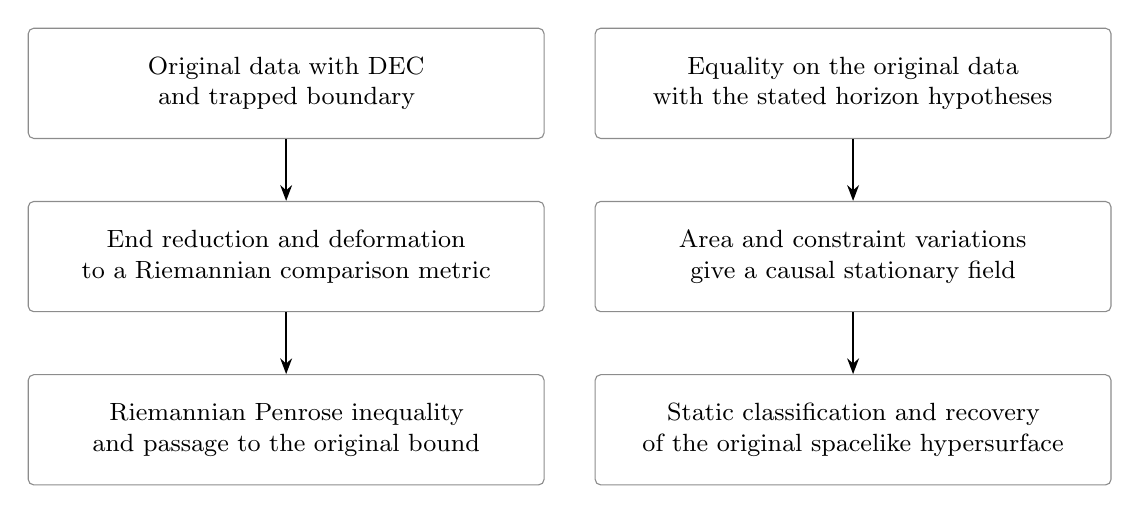
\begin{tikzpicture}[
  box/.style={draw=black!45,rounded corners=2pt,align=center,
    text width=6.2cm,minimum height=14mm,inner sep=5pt,font=\small},
  arr/.style={-{Stealth[length=2mm]},thick}]
\node[box] (data) at (0,0) {Original data with DEC\\and trapped boundary};
\node[box] (deform) at (0,-2.2) {End reduction and deformation\\to a Riemannian comparison metric};
\node[box] (bound) at (0,-4.4) {Riemannian Penrose inequality\\and passage to the original bound};
\node[box] (equal) at (7.2,0) {Equality on the original data\\with the stated horizon hypotheses};
\node[box] (field) at (7.2,-2.2) {Area and constraint variations\\give a causal stationary field};
\node[box] (recover) at (7.2,-4.4) {Static classification and recovery\\of the original spacelike hypersurface};
\draw[arr] (data)--(deform);
\draw[arr] (deform)--(bound);
\draw[arr] (equal)--(field);
\draw[arr] (field)--(recover);
\end{tikzpicture}
\caption{The numerical comparison and the equality argument. The bound
proved on the left applies to the nearby data used in the variations on
the right. Rigidity is obtained from the original data.}
\label{intro:proof-routes}
\end{figure}


The anti-de Sitter proof uses the Taylor coefficients of the given
branch. Actual weighted remainder bounds connect those coefficients
to the mass and area. The quadratic coefficient is a nonnegative quadratic
form with a kernel of dimension four. A fourth-order argument treats its
nonradial directions,
while radial directions satisfy an exact mass conservation identity.
This part is independent of the asymptotically flat elliptic construction.

\subsection{Relation to earlier work}

Penrose proposed the mass--horizon comparison in the context of
gravitational collapse and cosmic censorship \cite{Penrose1973}.
For time-symmetric data, Huisken and Ilmanen proved the
connected-horizon inequality by weak inverse mean curvature flow,
and Bray proved the total-area bound for possibly disconnected
horizons by conformal flow \cite{HuiskenIlmanen2001,Bray2001}.
Bray and Lee extended the numerical Riemannian inequality to spatial
dimensions below eight; spin enters their higher-dimensional equality
statement \cite{BrayLee2009}. Ben-Dov's counterexample distinguishes
apparent-horizon area from minimum enclosing area \cite{BenDov2004}.
Carrasco and Mars constructed counterexamples for outermost generalized
apparent horizons \cite{CarrascoMars2010}.
Bray and Khuri developed a generalized Jang reduction, including
spherical existence results and conditional nonspherical constructions
\cite{BrayKhuri2010,BrayKhuri2011}.

Allen, Bryden, Kazaras, and Khuri obtained a universal suboptimal
mass--area bound in three dimensions under their decay and horizon
assumptions \cite{AllenBrydenKazarasKhuri2025}.
Khuri and Kunduri proved the sharp inequality for
$SU(n+1)$-invariant cohomogeneity-one data in spatial dimensions
$2(n+1)$ \cite{KhuriKunduri2025}.
The inequalities here have a different scope: the three- and
four-dimensional results impose no such symmetry, and use their
specified minimum enclosing quantities.

The stationary field arising from equality is related to the
variational study of ADM mass. Hirsch and Huang proved a strong
maximum principle for the norm of a causal Killing field and studied
mass minimizers with fixed Bartnik boundary data
\cite{HirschHuang2025}. Those boundary data and regularity hypotheses
differ from the area variations used here. Once static vacuum geometry
is obtained, the conformal-doubling method of Bunting and
Masood-ul-Alam provides the classical model for the classification
\cite{BuntingMasoodUlAlam1987}. We prove the completeness and
low-regularity zero-mass statement needed for our double.
Higher-dimensional static-vacuum uniqueness was developed by Gibbons,
Ida, and Shiromizu \cite{GibbonsIdaShiromizu2002}. Here the static geometry
and its complete base must first be recovered from the original initial data.
The charged and anti-de Sitter parts give the comparisons with
earlier results specific to those settings where their hypotheses
can be stated precisely.

\subsection{Reading conventions}

The five parts are ordered by their mathematical dependencies.
The three-dimensional numerical theorem precedes the global extension,
rigidity, and charged application. The four-dimensional part states its own normalizations and contains
both the numerical construction and original-data equality proof.
The anti-de Sitter part is independent and uses its own asymptotic
geometry. The entry points are
Sections~\ref{n3:intro:section}, \ref{n3:rigidity:setup},
\ref{ch:intro:charged-section}, \ref{four:sec:introduction}, and
\ref{ads:sec:setting}, respectively.
Within each analytic construction the geometry
and strictification are fixed before the deformation parameters.
Uniform polynomial estimates and regularity estimates at a fixed
parameter have distinct roles; the proofs specify the order of
exhaustion and limits where each is used.


\part{Three-dimensional initial data}
\section{Three-dimensional exterior data and the mass inequality}\label{n3:intro:section}

\subsection{Initial data, normals, and enclosing area}

We work in three spatial dimensions, with zero cosmological constant and
\(G=c=1\). For a Riemannian metric \(g\) and a symmetric covariant
two-tensor \(K\), define the constraint densities by
\begin{equation}\label{n3:intro:constraints}
 16\pi\mu=R_g+(\tr_gK)^2-|K|_g^2,\qquad
 8\pi J=\Div_g\bigl(K-(\tr_gK)g\bigr).
\end{equation}
Here \(J\) is a covector field. The dominant energy condition is
\begin{equation}\label{n3:intro:dec}
                         \mu\ge |J|_g.
\end{equation}
All initial data considered here are smooth, including at a compact
boundary when one is present.

On an asymptotically flat end with Euclidean coordinates \(x\) and
\(r=|x|\), our basic assumptions are
\begin{equation}\label{n3:intro:decay}
 g_{ij}-\delta_{ij}=O_2(r^{-q}),\qquad
 K_{ij}=O_1(r^{-1-q}),\qquad q>\tfrac12.
\end{equation}
The notation \(O_j(r^{-a})\) includes the corresponding coordinate
derivative bounds through order \(j\). We assume that \(\mu\) and
\(|J|_g\) are integrable and that the following ADM limits exist and are
finite:
\begin{align}
 E&=\frac1{16\pi}\lim_{r\to\infty}
   \int_{S_r}(\partial_jg_{ij}-\partial_i g_{jj})n^i
                    \dd A_\delta,\label{n3:intro:energy}\\
 P_i&=\frac1{8\pi}\lim_{r\to\infty}
   \int_{S_r}\bigl(K_{ij}-(\tr_gK)g_{ij}\bigr)n^j
                    \dd A_\delta.\label{n3:intro:momentum}
\end{align}
The normal and area form in these definitions are Euclidean. Whenever
\(E>|P|_\delta\), write
\begin{equation}\label{n3:intro:rest-mass}
                         m=\sqrt{E^2-|P|_\delta^2}.
\end{equation}

For a two-sided surface \(\Sigma\) with specified unit normal \(\nu\),
we use
\[
 H_\Sigma=\Div_\Sigma\nu,\qquad
 \theta_+(\Sigma)=H_\Sigma+\tr_\Sigma K.
\]
Thus Euclidean spheres have positive mean curvature for the normal
toward infinity. A future marginally outer trapped surface, abbreviated
MOTS, satisfies \(\theta_+=0\). A weakly future outer trapped surface
satisfies \(\theta_+\le0\). Our spacetime sign convention is
\begin{equation}\label{n3:intro:k-sign}
 K(Y,Z)=\mathbf g(\mathbf\nabla_Y n,Z),
\end{equation}
where \(n\) is the future unit timelike normal. Equivalently, in Gaussian
normal coordinates the spatial metric has normal derivative \(2K\).

\begin{definition}[Exterior and enclosing area]\label{n3:intro:exterior-class}
An exterior is a connected orientable smooth three-manifold \(\Omega\)
with nonempty compact smooth boundary, complete as a metric space with
its boundary included, and with exactly one end, which is asymptotically flat.
An enclosing cut is a compact smooth embedded surface in
\(\overline\Omega\) separating the entire inner boundary from the
sufficiently distant part of that end. Equivalently, it bounds the side
containing the distant end; the other side is filled up to the inner
obstacle. A cut may have several components and may coincide with the
inner boundary. Its normal points toward the end. We put
\[
 a_g(\partial\Omega)=
  \inf\{|\Gamma|_g:\Gamma\text{ is an enclosing cut}\}.
\]
When using perimeter compactness, we take the closure of this class
among filled inner sets and include the area of any frontier coinciding
with the obstacle. Smooth outward approximation gives the same
infimum. Enclosing cuts and minimizing sets are taken with bounded
complementary pockets filled. Auxiliary perimeter arguments may use
competitors containing the inner obstacle before filling: filling a bounded
pocket deletes its frontier, cannot increase perimeter, and leaves the enclosing
infimum unchanged.
\end{definition}

The definition permits coincidence because first variations of the
minimum need not be realized by a cut lying strictly outside the
obstacle. It permits disconnected cuts because neither the minimizing
hull nor an intermediate trapped boundary need be connected. The
perimeter formulation and its compactness properties are established
in Section~\ref{n3:reduction:section}.

\subsection{The one-ended exterior inequality}

\begin{theorem}[Minimum-enclosing-area inequality]\label{n3:intro:exterior-inequality}
Let \((\Omega,g,K)\) be an exterior as in
Definition~\ref{n3:intro:exterior-class}. Assume
Equations~\eqref{n3:intro:constraints}--\eqref{n3:intro:decay}, integrability
of \(\mu\) and \(|J|_g\), and the finite ADM limits
\eqref{n3:intro:energy}--\eqref{n3:intro:momentum}. Orient \(\partial\Omega\)
by the normal into \(\Omega\), and suppose
\(\theta_+(\partial\Omega)\le0\). If \(E>|P|_\delta\), then
\begin{equation}\label{n3:intro:penrose}
          \sqrt{E^2-|P|_\delta^2}
               \ge \sqrt{\frac{a_g(\partial\Omega)}{16\pi}}.
\end{equation}
No extension of the data across \(\partial\Omega\) is required.
\end{theorem}

\section{Exterior approximation and reduction to a rest end}
\label{n3:reduction:section}

We reduce the invariant-mass inequality to an energy inequality on a
controlled rest end.  We replace the distant end, bend the replacement
inside Schwarzschild spacetime, and repair its constraint deficit with a
conformal change of vanishing mass cost.  Throughout,
$(N,g,K)$ is a smooth exterior with one asymptotically flat end and compact
smooth boundary $B$.  The normal $\nu$ on $B$ points into $N$.  Completeness
means completeness up to this boundary.  We assume
\begin{equation}
\label{n3:reduction:original-decay}
 g-\delta=O_2(r^{-q}),\qquad K=O_1(r^{-1-q}),\qquad q>\tfrac12,
\end{equation}
and the integrability and dominant energy condition of
Theorem~\ref{n3:intro:exterior-inequality}.  The symbol $a_g(B)$ denotes the
filled enclosing perimeter infimum specified there.  None of the results
in this section requires the boundary to be connected or outermost.

\subsection{A strict conformal direction}

\begin{lemma}[Conformal constraint formulas]
\label{n3:reduction:conformal-formulas}
For a smooth function $f$, set
\[
 g_f=e^{4f}g,\qquad K_f=e^{2f}K.
\]
The corresponding constraint densities satisfy
\begin{align}
 16\pi e^{4f}\mu_f
   &=16\pi\mu-8\Delta_g f-8|df|_g^2,
       \label{n3:reduction:conformal-energy}\\
 8\pi J_f
   &=e^{-2f}\bigl(8\pi J+4K(\nabla f,\cdot)\bigr).
       \label{n3:reduction:conformal-momentum}
\end{align}
Here the second identity is an identity of covectors.  Consequently,
\begin{align}
 16\pi e^{4f}(\mu_f-|J_f|_{g_f})
 \ge{}&16\pi(\mu-|J|_g)\notag\\
 &+8\bigl(-\Delta_g f-|df|_g^2-|K|_g|df|_g\bigr).
       \label{n3:reduction:conformal-dec}
\end{align}
On the fixed boundary,
\begin{equation}
 \theta_{+,f}=e^{-2f}(\theta_++4\partial_\nu f).
       \label{n3:reduction:conformal-expansion}
\end{equation}
Equivalently, if $u=e^f>0$, the last summand in
Equation~\eqref{n3:reduction:conformal-dec} is
$8u^{-1}(-\Delta_g u-|K|_g|du|_g)$.
\end{lemma}

\begin{proof}
The scalar-curvature transformation in dimension three is
$e^{4f}\Scal_{g_f}=\Scal_g-8\Delta_g f-8|df|^2$.
Both quadratic terms in $K$ scale by $e^{-4f}$, which proves
Equation~\eqref{n3:reduction:conformal-energy}.
Put $\pi=K-(\tr_gK)g$.  Then
$\pi_f=e^{2f}\pi$.  For a covariant symmetric tensor $T$, the connection
difference for $\widetilde g=\Omega^2g$ gives, in dimension three,
\[
 \widetilde\nabla^{,i}(\Omega T)_{ij}
 =\Omega^{-1}\bigl(\nabla^iT_{ij}
          +2T_{ij}\nabla^i\log\Omega
          -(\tr_gT)\partial_j\log\Omega\bigr).
\]
Take $\Omega=e^{2f}$ and use $\tr_g\pi=-2\tr_gK$.
The terms containing $\tr_gK$ cancel, leaving
Equation~\eqref{n3:reduction:conformal-momentum}.  Taking its norm introduces
another factor $e^{-2f}$.  The triangle inequality, with the factor two
between the constraint normalizations $16\pi$ and $8\pi$, yields
Equation~\eqref{n3:reduction:conformal-dec}.
Finally, $\nu_f=e^{-2f}\nu$,
$H_f=e^{-2f}(H+4\partial_\nu f)$, and
$\tr_{B,g_f}K_f=e^{-2f}\tr_{B,g}K$.  This proves
Equation~\eqref{n3:reduction:conformal-expansion}.  The last assertion follows
from $\Delta\log u+|d\log u|^2=u^{-1}\Delta u$.
\end{proof}

\begin{lemma}[Strict direction under the original decay]
\label{n3:reduction:strict-direction}
Choose
\[
 0<\delta<\beta<\min(q,1).
\]
There are smooth positive functions $w$ and $\phi$ on $N$, with
$w=r^{-3-\delta}$ on the end, such that
\begin{align}
 &\partial_\nu\phi=-1\quad\hbox{on }B,
       &\phi&=O_2(r^{-1}),\label{n3:reduction:strict-boundary}\\
 &-\Delta_g\phi-|K|_g|d\phi|_g\ge w,
       &\frac{-\Delta_g\phi}{w}&\longrightarrow1.
       \label{n3:reduction:strict-source}
\end{align}
The Euclidean normal flux
\[
 L_\phi=\lim_{r\to\infty}
          \int_{S_r}\partial_r\phi\,\dd A_\delta
\]
is finite and negative.  For every finite $s\ge0$, set
\begin{equation}
 \label{n3:reduction:linear-family}
 u_s=1+s\phi,\qquad g_s=u_s^4g,\qquad K_s=u_s^2K.
\end{equation}
These data are complete up to $B$ and satisfy DEC, strictly for $s>0$.
If $\theta_+\le0$ on $B$, their boundary expansion remains nonpositive
and is strictly negative for $s>0$.  Their decay exponent can be taken to be
$\min(q,1)>1/2$, their constraint densities are integrable, and
\begin{equation}
 \label{n3:reduction:strict-charges}
 E_s=E+sA_\phi,\qquad P_s=P,
 \qquad A_\phi=-\frac{L_\phi}{2\pi}>0.
\end{equation}
Their full enclosing infima satisfy
\begin{equation}
 \label{n3:reduction:strict-areas}
 a_g(B)\le a_{g_s}(B)
       \le (1+s\|\phi\|_\infty)^4a_g(B).
\end{equation}
In particular $E_s\to E$ and $a_{g_s}(B)\to a_g(B)$ as $s\downarrow0$.
No sign assumption on the ADM vector is needed.

If $K$ is compactly supported and the metric has symbol estimates of all
orders with $g-\delta=O(r^{-1})$, the function can instead be chosen with
$\phi=O_k(r^{-1})$ for every $k$, while retaining
Equations~\eqref{n3:reduction:strict-boundary} and
\eqref{n3:reduction:strict-source}.
\end{lemma}

\begin{proof}
Choose smooth $b\ge|K|_g$, positive everywhere and equal to
$b_0r^{-1-\beta}$ sufficiently far out, where $b_0>0$ is chosen large
enough.  This is possible because $\beta<q$.  Choose a smooth positive
regularizer $\zeta$, equal to $r^{-2}$ on the end, and extend $w$ smoothly
and positively to $N$.  We solve
\begin{equation}
 \label{n3:reduction:drift-poisson}
 -\Delta_g\phi=b\sqrt{|d\phi|_g^2+\zeta^2}+w,
 \qquad \partial_\nu\phi=-1,
 \qquad \phi\longrightarrow0.
\end{equation}
The regularizer makes this equation smooth even at critical points.

First truncate at a large coordinate sphere $S_R$ and prescribe
$\phi=0$ there.  The Neumann and Dirichlet conditions occur on disjoint
boundary components.  For $0\le t\le1$, replace $b$ in
Equation~\eqref{n3:reduction:drift-poisson} by $tb$.  At $t=0$, the mixed
Laplacian is invertible: its Dirichlet face gives the Poincare inequality,
and the weak solution obtained from its coercive quadratic form is smooth
by boundary regularity.  At any solution, the linearization is a
Laplacian with a smooth drift of norm at most $b$ and with the homogeneous
mixed boundary conditions.  The strong maximum principle and the Hopf
boundary principle make its kernel zero.  It is a Fredholm perturbation
of the mixed Laplacian of index zero, and is therefore invertible.
The boundary estimates used here are the ordinary elliptic estimates
for Dirichlet and normal Neumann conditions: positive definiteness of
$g$ verifies their principal complementing condition, and the disjoint
boundary components can be covered separately
\cite{AgmonDouglisNirenberg1959}.  The maximum principles and local
elliptic estimates below are used in their usual uniformly elliptic
forms \cite{GilbargTrudinger2001}.

To close continuation at $t=1$, first work on a fixed truncation.
The elliptic $W^{2,p}$ estimate
and gradient interpolation give
\[
 \|\phi\|_{W^{2,p}}
 \le C_p\bigl(1+\|\phi\|_{L^p}+\|d\phi\|_{L^p}\bigr)
 \le \tfrac12\|\phi\|_{W^{2,p}}
       +C'_p(1+\|\phi\|_{L^p}).
\]
The constants include the fixed boundary data and are uniform in $t$.
If the supremum norms of solutions on this truncation were unbounded,
divide them by their supremum norms.  The preceding estimate with
$p>3$, compactness, and the equation give a nonzero limit $v$ with
homogeneous mixed data satisfying
\[
 -\Delta_gv=t_*b|dv|_g.
\]
This can be written $\Delta_gv+A\cdot dv=0$ with a bounded measurable
drift: take $A=t_*b\nabla v/|dv|$ off the critical set and zero on it.
The strong and Hopf maximum principles exclude a nonzero solution with
the homogeneous mixed conditions.  Thus the supremum norms are bounded.
The $W^{2,p}$ estimate, Schauder estimates, and the smooth equation now
give the bounds needed for closedness of continuation.  Existence on
each truncation follows.

Every such solution is nonnegative.  A negative minimum cannot be
interior because the right side of
Equation~\eqref{n3:reduction:drift-poisson} is positive.  At an inner-boundary
minimum, the outward-domain derivative would be negative by the Hopf
principle, whereas the prescribed derivative in that direction is $1$.
The outer value is zero.

It remains to make these bounds independent of $R$.  For fixed sufficiently large
$A$ and then sufficiently large $r_0$, the positive radial function
\[
 v_0(r)=r^{-1}(1-Ar^{-\delta})
\]
satisfies, on $r\ge r_0$,
\begin{align*}
 -\Delta_gv_0-b|dv_0|_g
 &=A\delta(1+\delta)r^{-3-\delta}
       +O(r^{-3-q})+O(r^{-3-\beta})\ge c_0w.
\end{align*}
The constants are fixed independently of the truncation.  Since
$b\zeta=o(w)$, a sufficiently large multiple of $v_0$ is a supersolution
of the regularized equation.  The comparison principle gives
\begin{equation}
 \label{n3:reduction:core-barrier}
 0\le\phi(x)\le C(1+M_R)v_0(r),\qquad
 M_R=\sup_{N\cap\{r\le r_0\}}\phi,
 \quad r_0\le r\le R.
\end{equation}
The notation for the compact core includes all points outside the end
chart.  Were $M_R$ unbounded along expanding truncations, the normalized
solutions $\phi/M_R$ would have locally uniform $W^{2,p}$ bounds, including
at $B$, by the preceding local estimates and
Equation~\eqref{n3:reduction:core-barrier}.  A subsequence would converge
locally in $C^1$ to a nonnegative function with maximum one on the core,
homogeneous inner Neumann data, and a bounded-drift homogeneous equation.
Equation~\eqref{n3:reduction:core-barrier} makes its value tend to zero at
infinity.  It consequently attains a positive maximum, contradicting the
strong or Hopf principle for that homogeneous equation.  This proves the
uniform core bound.  The contradiction uses the homogeneous bounded-drift
equation.

Local compactness and diagonal extraction give a smooth solution of
Equation~\eqref{n3:reduction:drift-poisson}, with $\phi=O(r^{-1})$.
The claimed derivative count can be checked directly on annuli.  Put
\[
 \phi_{\rho}(y)=\rho\phi(\rho y),\qquad
 g_{\rho}(y)=g(\rho y),\qquad 1<|y|<4.
\]
On smaller fixed annuli the equation is
\[
 -\Delta_{g_{\rho}}\phi_{\rho}
 =\rho b(\rho y)
       \sqrt{|d\phi_{\rho}|_{g_{\rho}}^2+
                     (\rho^2\zeta(\rho y))^2}
       +\rho^3w(\rho y).
\]
Its coefficients have uniform $C^{1,1}$ bounds from the two derivatives
in Equation~\eqref{n3:reduction:original-decay}; the scaled drift is
$O(\rho^{-\beta})$ and the scaled source is $O(\rho^{-\delta})$.
The bounded zeroth-order norm, interior $W^{2,p}$ estimates, and gradient
interpolation first give uniform $C^{1,\alpha}$ bounds for some
$\alpha>0$.  The right side is then uniformly $C^\alpha$.  Schauder
estimates give uniform $C^{2,\alpha}$ bounds on smaller annuli.  This
proves $\phi=O_2(r^{-1})$ without using a third derivative of $g$ or a
second derivative of $K$.

The right side of Equation~\eqref{n3:reduction:drift-poisson} is
$w+O(r^{-3-\beta})$.  It is integrable and proves
Equation~\eqref{n3:reduction:strict-source}.  The divergence theorem, with
outward-domain normal $-\nu$ on $B$, gives
\begin{equation}
 \label{n3:reduction:phi-flux}
 \lim_{r\to\infty}\int_{S_r}\partial_{n_g}\phi\,\dd A_g
 =-|B|_g-\int_N
       \bigl(b\sqrt{|d\phi|_g^2+\zeta^2}+w\bigr)\,\dd V_g.
\end{equation}
The Euclidean flux differs by $O(r^{-q})$ and has the same finite limit.

For every fixed finite $s\ge0$, the factor $u_s$ in
Equation~\eqref{n3:reduction:linear-family} is bounded and at least one,
so the transformed data are complete up to $B$.
The $u$-form of Lemma~\ref{n3:reduction:conformal-formulas} gives
\begin{align*}
 16\pi u_s^4(\mu_s-|J_s|_{g_s})
 &\ge16\pi(\mu-|J|_g)
        +\frac{8s}{u_s}(-\Delta_g\phi-|K|_g|d\phi|_g)
 \ge \frac{8s}{u_s}w,\\
 \theta_{+,s}
 &=u_s^{-2}\left(\theta_+-\frac{4s}{u_s}\right).
\end{align*}
This proves the asserted signs for all finite $s$, without a smallness
restriction.

Since $u_s-1=O_2(r^{-1})$, the transformed decay exponent is
$\min(q,1)>1/2$.  The exact energy transformation is
\[
 16\pi u_s^4\mu_s=16\pi\mu-8s u_s^{-1}\Delta_g\phi.
\]
Here $\Delta_g\phi=O(r^{-3-\delta})$, and the additional current term
is bounded by a fixed-$s$ constant times
$|K|_g|d\phi|_g=O(r^{-3-q})$.  Both are integrable in dimension three.
The bounded positive conformal factor also preserves integrability in
the transformed volume measure.

The leading metric change is $4s\phi\delta$, whose ADM energy flux
is $-8s\int_{S_r}\partial_r\phi\,\dd A_\delta$ before division by
$16\pi$.  All remaining metric flux terms are
$O_s(r^{-q})+O_s(r^{-1})$.  Writing $\pi=K-(\tr_gK)g$, one has
$\pi_s=u_s^2\pi$, so the change in its Euclidean momentum flux is
$O_s(r^2r^{-1}r^{-1-q})=O_s(r^{-q})$.
This proves Equation~\eqref{n3:reduction:strict-charges};
Equation~\eqref{n3:reduction:phi-flux} gives $A_\phi>0$.
No $1/r$ coefficient expansion for $\phi$ is needed.
Finally, the cut class is unchanged and every cut has area
$\int_\Gamma u_s^4\,\dd A_g$.  Bounding $u_s$ between $1$ and
$1+s\|\phi\|_\infty$ and taking infima proves
Equation~\eqref{n3:reduction:strict-areas}, including coincident and
disconnected cuts.

For the final assertion, take $b$ nonnegative, compactly supported, and
at least $|K|$; the proof is unchanged.  The end equation is then simply
$-\Delta_g\phi=w$.  Once the two-derivative estimate has been established,
successive annular elliptic estimates use the assumed symbol bounds for
$g$ and $w$ to give $\phi=O_k(r^{-1})$ for every $k$.
\end{proof}

\subsection{Compactness of enclosing minimizers}

The end replacement will change the metric on receding annuli.  The next
lemma keeps area-minimizing enclosures in a fixed compact set, where local
metric convergence controls their areas.

\begin{lemma}[Enclosing areas under receding changes]
\label{n3:reduction:area-compactness}
Let $g_j$ be smooth metrics on the fixed exterior $N$, converging to $g$
locally uniformly up to $B$.  Suppose that in a fixed chart outside a
compact set they satisfy, with constants independent of $j$,
\begin{equation}
 \label{n3:reduction:area-geometry}
 c\delta\le g_j\le C\delta,\qquad r|\partial g_j|_\delta\le C.
\end{equation}
Suppose also that each $g_j$ has an asymptotically flat end, possibly
in a different chart, and admits a fixed compact enclosing competitor
with uniformly bounded area.  Then minimizing filled enclosures exist,
their boundaries lie in one fixed compact subset of $N$, and
\[
 a_{g_j}(B)\longrightarrow a_g(B).
\]
The perimeter and smooth enclosing infima agree.  Each minimizing
boundary is $C^{1,1}$, and is smooth minimal away from contact with $B$.
\end{lemma}

\begin{proof}
For purposes of perimeter minimization only, extend the metrics through
a collar of $B$ and attach a fixed compact filling.  The filling need not
satisfy any constraint or curvature condition.  Extend $g_j$ so that the
extensions converge uniformly on this fixed collar and filling.  A filled
enclosure is then a bounded set containing the prescribed inner obstacle.

For each fixed metric, sufficiently large spheres in its asymptotically
flat chart have strictly positive outward mean curvature.  Clipping a
bounded enclosure at any such sphere cannot increase perimeter.  To see
this, integrate the divergence of the outward unit normal field of the
sphere foliation over the part of the enclosure outside the sphere.  Its
divergence is positive.  Its flux through the exterior boundary is at
most the area of that boundary, whereas its flux on the cutting sphere
is the negative of the new cutting area.  Thus the discarded boundary
area is at least the inserted area.  Approximation gives the same
statement for finite-perimeter sets.  The direct method on the resulting
bounded domain now gives a minimizer.  The clipping observation makes
this a minimizer against every bounded competitor, not merely those
inside the chosen truncation.

Off the obstacle the boundary is locally perimeter minimizing.  If it
contains a point of radius $r$ sufficiently large, the coordinate ball
of radius $c_1r$ about that point avoids the obstacle.  After scaling
this ball to unit size, Equation~\eqref{n3:reduction:area-geometry} gives
uniform ellipticity and uniform first-derivative bounds for its area
integrand.  The local perimeter density estimate gives
\[
 \operatorname{Area}_{g_j}
       (\partial F_j\cap B_{c_1r})\ge c_2r^2.
\]
Here $c_1,c_2>0$ are independent of $j$ and $r$.  One may obtain this
estimate from the relative isoperimetric inequality and the comparison
which removes, or fills, the set in concentric balls; integration of the
resulting differential inequality gives the area lower bound.  The
fixed competitor bounds the left side above independently of $j$.
Consequently the minimizing boundaries lie in a fixed compact set.

Perimeter compactness now gives a limiting filled enclosure.  Uniform
metric convergence on that compact set and lower semicontinuity imply
\[
 a_g(B)\le\liminf_j a_{g_j}(B).
\]
Conversely, using a fixed enclosure with $g$-area arbitrarily close to
$a_g(B)$ gives the reverse upper-limit inequality.

The local obstacle regularity theorem for pure area minimization with
a $C^2$ obstacle gives $C^{1,1}$ regularity, and smoothness off contact,
in dimension three; its local estimates require only the appropriate
bounded geometry of the smooth metric
\cite[Regularity Theorem 1.3]{HuiskenIlmanen2001}.
This applies to the fixed smooth obstacle and our smooth one-sided
metrics after the collar extension.  Finally, push a minimizing boundary
slightly away from its contact set by a smooth vector field agreeing
there with the outward obstacle normal.  In a small obstacle collar its
flow increases the signed distance to the obstacle.  The resulting
$C^1$ embedded boundary is a positive distance from the obstacle.
Smooth local graph approximation, within that distance, preserves
enclosure and changes area by an arbitrarily small amount.  This proves
equality of the smooth and perimeter infima and also justifies using
smooth fixed competitors in the upper-limit argument.
\end{proof}

\subsection{Schwarzschild reference charges}

We next construct the vacuum end used in the replacement.  Its charges
must agree with those of the original data before we bend it to a rest
slice.

\begin{lemma}[A reference end with prescribed timelike charges]
\label{n3:reduction:boosted-reference}
Let $E>|P|$ and $m=(E^2-|P|^2)^{1/2}$.  There is a spacelike plane
near spatial infinity of Schwarzschild spacetime of mass $m$ whose
induced data, in asymptotically Euclidean coordinates on the plane,
have ADM charges $(E,P)$.  The reference data satisfy
\[
 g_*-\delta=O_k(r^{-1}),\qquad K_*=O_k(r^{-2})
\]
for every derivative order $k$.
\end{lemma}

\begin{proof}
In static isotropic coordinates $(T,y)$ the Schwarzschild metric is
\begin{equation}
 \label{n3:reduction:schwarzschild-spacetime}
 -\left(\frac{1-m/(2r)}{1+m/(2r)}\right)^2\dd T^2
       +\left(1+\frac{m}{2r}\right)^4\delta_{ij}\dd y^i\dd y^j,
 \qquad r=|y|.
\end{equation}
Its perturbation $h$ from Minkowski space has symbol decay $r^{-1}$
on every fixed spacelike cone.  Constant Lorentz transformations preserve
this decay.  We verify the transformation of the ADM charges directly.

In inertial coordinates for the background Minkowski metric $\eta$, put
\begin{align}
 \mathcal F_{\ell ab}
  ={}&\partial_a h_{\ell b}-\partial_\ell h_{ab}\notag\\
   &+\eta_{\ell b}
       (\partial^d h_{ad}-\partial_a\tr_\eta h)
    -\eta_{ab}
       (\partial^d h_{\ell d}-\partial_\ell\tr_\eta h).
       \label{n3:reduction:superpotential}
\end{align}
This tensor is antisymmetric in its first two slots, and differentiation
of the displayed formula gives
$\partial^\ell\mathcal F_{\ell ab}=2G^{\mathrm{lin}}_{ab}$.
The exact Einstein tensor vanishes; its terms beyond the linearization
are $O(r^{-4})$.  Thus this divergence is $O(r^{-4})$.

Use an inertial frame in which the plane under consideration is
$x^0=0$.  With $\eta=\operatorname{diag}(-1,1,1,1)$, direct substitution
in Equation~\eqref{n3:reduction:superpotential} gives
\begin{align*}
 \mathcal F_{i00}&=\partial_jh_{ij}-\partial_ih_{jj},\\
 \mathcal F_{i0k}
  &=2\bigl(K^{\mathrm{lin}}_{ik}
          -\delta_{ik}\tr K^{\mathrm{lin}}\bigr)
       +\partial_kh_{0i}-\delta_{ik}\partial_jh_{0j},
\end{align*}
where
\[
 K^{\mathrm{lin}}_{ik}
 =\tfrac12(\partial_0h_{ik}-\partial_ih_{0k}-\partial_kh_{0i}).
\]
The convention is the normal rate of the spatial metric divided by two.
For fixed $k$, the final vector has zero flux through every closed sphere.
Indeed it equals
\[
 \partial_j(\delta_{jk}h_{0i}-\delta_{ik}h_{0j}),
\]
the divergence of a tensor antisymmetric in $i,j$.  This zero-flux
identity is local to a neighborhood of the sphere: extend the potential
smoothly inside before applying the divergence theorem, if necessary.
The nonlinear errors in the induced metric and second fundamental form
give vanishing flux errors.  Therefore the limiting fluxes of
$\mathcal F_{i0b}$ are $16\pi(E,P)$.

These fluxes are the integrals of the dual two-form of the first two
slots of $\mathcal F$, with its translation slot held fixed.  They
therefore transform tensorially under a constant Lorentz change of
frame.  Independence of the limiting spacelike cut follows directly
from Stokes' theorem: two large cuts on planes of slopes bounded
strictly below one can be joined within a fixed spacelike cone by a
three-dimensional cylinder of volume $O(R^3)$, all of whose points have
radius comparable to $R$.  Its divergence error is $O(R^{-4})$, so the
flux difference is $O(R^{-1})$.  Replacing the resulting ellipsoidal cuts
by coordinate spheres on either plane gives the same estimate.  The
limiting translation charges consequently transform by the Lorentz
representation.  The static plane has charges $(m,0)$, as follows by
inserting Equation~\eqref{n3:reduction:schwarzschild-spacetime} into the ADM
integral.  Its Lorentz orbit is precisely the set of future timelike
vectors of norm $m$, proving the assertion.

More explicitly the plane can be written $T=v\cdot y$, $|v|<1$.
Writing $y=Ax$, where
$A=(I-v\otimes v)^{-1/2}$, makes the induced Minkowski metric in the
$x$ coordinates equal to $\delta$.  The displayed decay then follows
from the symbol estimates in
Equation~\eqref{n3:reduction:schwarzschild-spacetime} and the formula for
the second fundamental form.  These coordinates will be used when
identifying the reference end with the given end.
\end{proof}

\subsection{Moments and compact linear corrections}

All operators in the next two lemmas are Euclidean.  For symmetric
covariant tensors define
\begin{equation}
 \label{n3:reduction:linear-operators}
 \mathcal Lh=\partial_i\partial_jh_{ij}-\Delta\tr h,
 \qquad
 (\mathcal Dk)_i=\partial_j(k_{ij}-(\tr k)\delta_{ij}).
\end{equation}
The formal adjoint kernel of $\mathcal L$ consists of affine functions;
the formal adjoint kernel of $\mathcal D$ consists of Euclidean Killing
fields.  Orthogonality to these kernels is the compatibility condition
for the compact inverses below.

\begin{lemma}[Compact scalar and symmetric divergence inverses]
\label{n3:reduction:compact-inverses}
Let $\mathcal A\subset\R^3$ be a fixed connected open annulus and let
$Q\Subset\mathcal A$.  Smooth sources supported in $Q$ admit the
following compact corrections, supported in a fixed larger compact
subset of $\mathcal A$.
\begin{enumerate}[label=\textup{(\roman*)}]
\item If $\int f=0$ and $\int x^if=0$ for $i=1,2,3$, there is a smooth
      symmetric tensor $h$ with $\mathcal Lh=f$ and
      $\|h\|_{W^{k+2,p}}\le C_{k,p}\|f\|_{W^{k,p}}$.
\item If $\int V\cdot Y=0$ for every Euclidean Killing field $Y$, there
      is a smooth symmetric tensor $k$ with $\mathcal Dk=V$ and
      $\|k\|_{W^{k_0+1,p}}\le C_{k_0,p}\|V\|_{W^{k_0,p}}$.
\end{enumerate}
The estimates hold for integers $k,k_0\ge0$ and $1<p<\infty$.
\end{lemma}

\begin{proof}
We first record the ordinary divergence inverse being used.  On a ball,
the regularized Bogovskii operator solves $\Div u=f$ for a mean-zero
compactly supported source, preserves compact support, and gains one
derivative in $W^{k,p}$; see
\cite[\S3.1, Equation~(3.13), Theorem~3.2, Corollary~3.4, and Remark~3.5]{CostabelMcIntosh2010}.
To apply it on the annulus, cover $Q$ by finitely
many balls compactly contained in $\mathcal A$, adding finitely many
overlapping balls so that the overlap graph is connected.  Partition the
source among the balls.  On a spanning tree of the overlap graph, pass
each piece's integral to its parent by subtracting and adding that
integral times a fixed unit-integral bump in the overlap.  Starting at
the leaves leaves every piece with zero integral; the root does also
because the total integral vanishes.  The decomposition has bounded
Sobolev norms because all cutoffs and bumps are fixed.  The sum of the
ball inverses gives a compact inverse on the annulus.  For sources in a
fixed compact set its output support lies in another fixed compact set.
This construction may be repeated twice using slightly enlarged compact
sets still contained in $\mathcal A$.

For the scalar assertion, solve $\partial_i u_i=f$ compactly.
Integration by parts gives
\[
 \int u_i=-\int x^if=0.
\]
Apply the divergence inverse to each component of $u$, obtaining
$\partial_j A_{ij}=u_i$.  Symmetrizing $A$ does not change its double
divergence.  Denote this symmetric matrix by $S$ and put
\[
 h=S-\tfrac12(\tr S)\delta.
\]
Since $h-(\tr h)\delta=S$, its linearized scalar curvature is $f$.
The two applications of the divergence inverse give the two-derivative
gain.

For the vector assertion, translation orthogonality gives
$\int V_i=0$.  Solve $\partial_jB_{ij}=V_i$ componentwise.  Orthogonality
to rotations and integration by parts imply
\[
 0=\int(x^jV_i-x^iV_j)
   =-\int(B_{ij}-B_{ji}).
\]
Thus the skew part $S_{ij}=(B_{ij}-B_{ji})/2$ has zero integral.  Apply
the divergence inverse to its independent components to obtain a tensor
$D$, skew in its first two indices, such that
$\partial_kD_{ijk}=-S_{ij}$.  Define
\begin{equation}
 \label{n3:reduction:stress-symmetrization}
 C_{ijk}=D_{ijk}-D_{ikj}-D_{jki}.
\end{equation}
Index interchange shows both
$C_{ijk}=-C_{ikj}$ and
$(C_{ijk}-C_{jik})/2=D_{ijk}$.  Consequently
\[
 T_{ij}=B_{ij}+\partial_kC_{ijk}
\]
is symmetric and satisfies $\partial_jT_{ij}=V_i$.  The last statement
uses the skew symmetry in $j,k$ to cancel the double divergence of $C$.
Set $k=T-(\tr T)\delta/2$ to invert trace reversal.  The first inverse
gains one derivative, the second gains another, and the last derivative
of $C$ leaves a net gain of one.  All constructions preserve smoothness
and have the stated support and norm bounds.
\end{proof}

\begin{lemma}[Integrable sources give sublinear first moments]
\label{n3:reduction:moment-estimates}
For data satisfying Equation~\eqref{n3:reduction:original-decay} and
integrable $\mu,|J|$, put $h=g-\delta$ and
$\pi=K-(\tr_\delta K)\delta$.  Then
\begin{align}
 \mathcal Lh&=16\pi\mu+O(r^{-2-2q}),\notag\\
 \partial_j\pi_{ij}&=8\pi J_i+O(r^{-2-2q}).
       \label{n3:reduction:linear-source-integrability}
\end{align}
In particular these Euclidean sources are integrable.  Their scalar
boundary fluxes paired with affine functions having zero constant term,
and their vector boundary fluxes paired with rotational Killing fields,
are $o(R)$ on coordinate spheres of radius $R$.
\end{lemma}

\begin{proof}
The scalar-curvature expansion has remainder bounded by
\[
 C\bigl(|h||\partial^2h|+|\partial h|^2+|K|^2\bigr),
\]
and the replacement of the momentum constraint by Euclidean divergence
has remainder bounded by
$C(|h||\partial K|+|\partial h||K|)$.  These are
$O(r^{-2-2q})$, using exactly the derivatives in
Equation~\eqref{n3:reduction:original-decay}.  They are integrable because
$2+2q>3$.

For any integrable function $F$ on the end and fixed $c>1$,
\begin{equation}
 \label{n3:reduction:sublinear-tail}
 \frac1R\int_{r_0<|x|<cR}|x|\,|F(x)|\,\dd x\longrightarrow0.
\end{equation}
Indeed the contribution inside any fixed radius $M$ tends to zero
after division by $R$; the remaining contribution is at most
$c\int_{|x|>M}|F|$.  Let $R\to\infty$ and then $M\to\infty$.

For an affine function $f$, the vector field
\[
 \mathcal Q_f(h)^i
  =f(\partial_jh_{ij}-\partial_i\tr h)
       -(\partial_jf)h_{ij}+(\partial_if)\tr h
\]
satisfies $\partial_i\mathcal Q_f(h)^i=f\mathcal Lh$.
For a Euclidean Killing field $Y$,
\[
 \partial_j(\pi_{ij}Y^i)=Y^i\partial_j\pi_{ij},
\]
because $\pi$ is symmetric.  Integrating from a fixed inner sphere and
using Equation~\eqref{n3:reduction:sublinear-tail} proves the asserted
$o(R)$ estimates.  This argument does not assert the existence of a
center-of-mass or angular-momentum limit and requires no parity
condition.
\end{proof}

\begin{proposition}[Annular replacement with a vanishing deficit]
\label{n3:reduction:annular-replacement}
Suppose $E>|P|$, and let $(g_*,K_*)$ be the reference end from
Lemma~\ref{n3:reduction:boosted-reference}, identified with the given end
in the common asymptotically Euclidean coordinates.  For all sufficiently
large $R$ there are smooth data $(\widetilde g_R,\widetilde K_R)$ equal to
$(g,K)$ on $r\le R$ and to $(g_*,K_*)$ on $r\ge4R$ such that
\begin{equation}
 \label{n3:reduction:annular-deficit}
 16\pi(\widetilde\mu_R-|\widetilde J_R|_{\widetilde g_R})
       \ge-\eta_RR^{-3},\qquad \eta_R\longrightarrow0.
\end{equation}
The possible negative part is supported in $R<r<4R$.
The metrics there are uniformly Euclidean comparable and have uniformly
bounded scaled first derivatives.  The construction uses no derivatives
of the original data beyond those in
Equation~\eqref{n3:reduction:original-decay} for its quantitative estimates.
\end{proposition}

\begin{proof}
Fix $\tfrac12<\beta<\min(q,1)$ and work on the annulus
$\mathcal A=\{1<|y|<4\}$ with $x=Ry$.  The scaled fields are
\[
 g_R(y)=g(Ry),\qquad k_R(y)=RK(Ry),
\]
and likewise for the reference data.  Their constraint densities are the
original densities multiplied by $R^2$.  If $h_R=g_R-\delta$, then
\begin{equation}
 \label{n3:reduction:scaled-smallness}
 \|h_R\|_{C^2(\mathcal A)}+\|k_R\|_{C^1(\mathcal A)}
 +\|h_{*,R}\|_{C^2(\mathcal A)}+\|k_{*,R}\|_{C^1(\mathcal A)}
 \le CR^{-\beta}.
\end{equation}
Choose $\chi\in C^\infty(\mathcal A)$ with $0\le\chi\le1$, equal to one near $|y|=1$ and zero
near $|y|=4$, with all its derivatives supported in a fixed compact
subannulus.  Blend both fields by this cutoff.

Write the constraints in the unnormalized form
\[
 \mathcal C(g,k)
 =\bigl(\Scal_g+(\tr_gk)^2-|k|_g^2,
             \Div_g(k-(\tr_gk)g)\bigr).
\]
Their Euclidean linear part is $(\mathcal Lh,\mathcal Dk)$.
On fields satisfying Equation~\eqref{n3:reduction:scaled-smallness}, the
nonlinear remainder is bounded in supremum norm by $CR^{-2\beta}$.
Thus the blended constraints equal the blended original constraint
sources, plus a quadratic error and the compact commutators
\begin{align*}
 f_R&=\mathcal L(\chi(h_R-h_{*,R}))
                      -\chi\mathcal L(h_R-h_{*,R}),\\
 V_R&=\mathcal D(\chi(k_R-k_{*,R}))
                      -\chi\mathcal D(k_R-k_{*,R}).
\end{align*}
They have $C^{0,1}$ norms at most $CR^{-\beta}$.  In detail the scalar
commutator applied to a symmetric tensor $h$ is
\begin{align*}
 &2\partial_i\chi(\partial_jh_{ij}-\partial_i\tr h)
       +(\partial_i\partial_j\chi)h_{ij}-(\Delta\chi)\tr h;
\end{align*}
one derivative of this expression uses at most two derivatives of $h$.
The vector commutator is $(\partial_j\chi)(k_{ij}-(\tr k)\delta_{ij})$;
one derivative uses at most one derivative of $k$.  No derivative of the
complete matter sources is needed.

Every affine moment of $f_R$ and every Killing-field moment of $V_R$
is $o(R^{-1})$.  For the constant moments, integration by parts on
$\mathcal A$ gives $R^{-1}$ times the difference between the physical
translation fluxes on its two boundary spheres, less the integrals of
the blended linear sources.  The flux difference tends to zero because
the reference and original ADM vectors agree.  Replacing the physical
momentum integrand by its Euclidean trace reversal costs
$O(R^{1-2q})$, which tends to zero.  By
Lemma~\ref{n3:reduction:moment-estimates}, the physical linear-source
integrals on this receding annulus tend to zero as well.
For a linear scalar test or a rotational vector test the corresponding
factor is $R^{-2}$.  Its physical boundary fluxes are $o(R)$ by the same
lemma, while the weighted source integrals are $o(R)$ by
Equation~\eqref{n3:reduction:sublinear-tail}.  This proves the claim.

Remove these small moments by fixed smooth bumps.  Explicitly, for a
basis $p_1,\ldots,p_4$ of affine functions and a fixed nonnegative bump
$\omega$ positive on a ball inside the annulus, the Gram matrix
\[
 G_{ab}=\int\omega p_ap_b
\]
is positive definite.  Subtract
$\omega\sum_{a,b}p_a(G^{-1})_{ab}\int p_bf_R$ from $f_R$.
For the vector moments use in exactly the same way the Gram matrix
$\int\omega Y_a\cdot Y_b$ of a basis of the six Euclidean Killing fields.
It too is positive definite, since a nonzero Killing field cannot vanish
on an open ball.  Both bump corrections have every fixed smooth norm
$o(R^{-1})$.

Apply Lemma~\ref{n3:reduction:compact-inverses} with the negative of the
moment-free commutators.  Since their $W^{1,p}$ norms are $O(R^{-\beta})$,
choosing $p>3$ gives metric and tensor corrections of size $O(R^{-\beta})$
in $W^{3,p}$ and $W^{2,p}$, respectively.  Sobolev embedding gives the
needed $C^{2,\alpha}$ and $C^{1,\alpha}$ bounds.  Their supports stay in
a fixed compact subset of $\mathcal A$.  Extend them by zero and undo
the scaling.  The metric remains positive definite for large $R$.

To check DEC, denote the original scaled sources by $(A_R,B_R)$, so
$A_R\ge2|B_R|_{g_R}$.  The reference sources vanish.  The corrected
sources therefore have the form
\[
 \bigl(\chi A_R,\chi B_R\bigr)
       +o(R^{-1})+O(R^{-2\beta})
\]
in supremum norm.  The norm of $B_R$ changes by at most
$CR^{-\beta}|B_R|\le CR^{-2\beta}$ when the metric is changed, since
the pointwise constraint formula gives $|B_R|\le CR^{-\beta}$.
All other nonlinear correction terms have the same quadratic bound.
Because $2\beta>1$, the scaled DEC deficit is $o(R^{-1})$.
Multiplication by $R^{-2}$ gives
Equation~\eqref{n3:reduction:annular-deficit}.  Outside the correction annulus
the data are either the original DEC data or the exact vacuum reference
data.  Smoothness follows from smoothness of the original fields and of
the compact inverse constructions, irrespective of the sizes of their
unneeded higher derivatives.
\end{proof}

\subsection{Bending to a rest slice and repairing the deficit}

\begin{lemma}[A vacuum bend with uniform geometry]
\label{n3:reduction:vacuum-bend}
The data in Proposition~\ref{n3:reduction:annular-replacement} can be
modified farther out, inside their exact Schwarzschild part, so that
they are induced by a constant-static-time slice outside a compact set.
This modification adds no constraint deficit.  Write $(g_R,K_R)$ for
the resulting unscaled data.  In the common end
coordinates the metrics are uniformly Euclidean comparable,
and throughout all transition annuli
\begin{equation}
 \label{n3:reduction:bend-geometry}
 |\partial g_R|_\delta+|K_R|_\delta\le C/r.
\end{equation}
There is a smooth proper radius $\rho_R$ on the end which equals the original
coordinate radius on the gluing annulus and equals the rest isotropic
radius beyond the transitions, with
\begin{equation}
 \label{n3:reduction:radius-geometry}
 c r\le\rho_R\le C r,\qquad
 |d\rho_R|_{g_R}^2\ge c,
 \qquad |\Delta_{g_R}\rho_R|\le C/r.
\end{equation}
All transition annuli lie between fixed multiples of $R$; the constants
can depend on the prescribed timelike ADM vector, but not on $R$.
\end{lemma}

\begin{proof}
Use the description $T=v\cdot y$, $y=Ax$, from
Lemma~\ref{n3:reduction:boosted-reference}.  Choose $R_b=c_bR$ so large,
with $c_b$ fixed, that the region $|y|\ge R_b$ is entirely inside the
exact reference part.  Let $\psi$ be a smooth function equal to one on
$(-\infty,0]$, zero on $[1,\infty)$, and taking values in $[0,1]$.
Replace the plane by the graph
\begin{equation}
 \label{n3:reduction:bending-graph}
 T_R(y)=(v\cdot y)
           \psi\left(\frac{\log(|y|/R_b)}{L}\right).
\end{equation}
Its Euclidean gradient satisfies
\[
 |dT_R|_\delta\le |v|\bigl(1+\|\psi'\|_\infty/L\bigr).
\]
Choose a fixed $L$ making the right side strictly smaller than one.
The lapse and spatial coefficients in
Equation~\eqref{n3:reduction:schwarzschild-spacetime} converge to their
Minkowski values, so for all sufficiently large $R$ this graph is
uniformly spacelike.  In fact for positive Schwarzschild mass the lapse
is smaller than one and the spatial conformal factor exceeds one,
which only improves this estimate on the static exterior.

The graph agrees with the original plane before $R_b$ and with a
constant-time slice after $e^LR_b$.  Its first derivative is bounded,
and its second and third derivatives are $O(r^{-1})$ and $O(r^{-2})$.
The induced metric is uniformly comparable with $\delta$; differentiating
its pullback formula gives the first bound in
Equation~\eqref{n3:reduction:bend-geometry}.  The second fundamental form
uses the graph's second derivatives and ambient first derivatives,
divided by a uniformly positive spacelikeness factor, and gives the
other bound.  These estimates remain true in the $x$ coordinates because
$A$ is a fixed invertible linear map.  The constraints vanish on the
entire bent part by the Gauss--Codazzi equations in exact vacuum
Schwarzschild spacetime.

It remains to make the radius precise.  On the bent region keep
$\rho_R=|x|=|A^{-1}y|$.  Beyond the bend, where the slice is already
static, write $y=r\omega$ and put $a(\omega)=|A^{-1}\omega|$.  Choose
$R_c$ a sufficiently large fixed multiple of $R_b e^L$, and a cutoff
$\chi_0$ equal to one before zero and zero after one.  In that static
region set
\[
 \rho_R(r,\omega)
 =r\exp\left[
    \chi_0\left(\frac{\log(r/R_c)}{L_0}\right)\log a(\omega)\right].
\]
For fixed sufficiently large $L_0$ its radial derivative is bounded
below by a positive constant: differentiating in $r$ gives the positive
factor $\rho_R/r$ times
$1+L_0^{-1}\chi_0'\log a$, which is at least $1/2$.
The function and its first two Euclidean derivatives have the bounds
$\rho_R\asymp r$, $|d\rho_R|\le C$, and
$|\partial^2\rho_R|\le C/r$.  Before this interpolation, the same
bounds hold for $|A^{-1}y|$, and uniform metric comparability gives the
gradient lower bound.  Combining these facts with
Equation~\eqref{n3:reduction:bend-geometry} proves
Equation~\eqref{n3:reduction:radius-geometry}.  After the interpolation,
$\rho_R=r$ is precisely the static isotropic radius.  All radius ratios
used in the construction are fixed, independently of $R$.
\end{proof}

\begin{lemma}[A radial DEC repair of vanishing mass cost]
\label{n3:reduction:radial-repair}
Consider the data obtained from
Proposition~\ref{n3:reduction:annular-replacement} and
Lemma~\ref{n3:reduction:vacuum-bend}.  There is a smooth positive conformal
factor $u_R$, constant on the unchanged inner region and tending to one
at infinity, such that $(u_R^4g_R,u_R^2K_R)$ satisfy DEC everywhere.
Moreover
\begin{equation}
 \label{n3:reduction:repair-size}
 \|u_R-1\|_\infty=o(R^{-1}),\qquad
 |du_R|=o(R^{-2})\quad\hbox{on the transition region}.
\end{equation}
The final end is exactly Schwarzschild with $K=0$ and mass
$m+o(1)$.  The boundary expansion retains its original weak sign.
\end{lemma}

\begin{proof}
All geometry estimates below are uniform in $R$.  Enlarge the fixed
transition region slightly so that, in terms of $t=\rho_R/R$, it lies
inside an interval $(a,b)$ with $0<a<b<\infty$.  Arrange that $t\ge b$
is in the static spherical region, and that the support of the possible
deficit lies in a fixed smaller interval $I\Subset(a,b)$.  Increasing
$b$ if needed makes these assertions follow from
Lemma~\ref{n3:reduction:vacuum-bend}.
We take $a=1$: the compact supports in the annular correction leave
a fixed neighborhood of $t=1$ free of deficit.  The factor constructed
below will consequently be constant throughout the original region
$r\le R$, and is extended by that constant over the compact core of $N$.

Let $\eta_R\to0$ be as in
Equation~\eqref{n3:reduction:annular-deficit}, replacing it by a positive
majorant if necessary.  We will choose $\varepsilon_R=C_0\eta_R$ and
construct
\[
 u_R=1+\frac{\varepsilon_R}{R}F_R(\rho_R/R),
\]
where $F_R$ and the relevant derivatives are bounded independently of
$R$.  Write $z_R=-F_R'$.  On $[a,b+1]$, initially define $z_R$ by
\begin{equation}
 \label{n3:reduction:repair-ode}
 z_R'=C_1z_R+\omega_1,
 \qquad z_R(a)=0,
\end{equation}
where $\omega_1$ is smooth, nonnegative, zero near $a$, and at least one
on $I$.  Take $C_1$ sufficiently large, depending only on the constants
in Equations~\eqref{n3:reduction:bend-geometry} and
\eqref{n3:reduction:radius-geometry}.  The solution is nonnegative and
has uniform bounds on this fixed interval.  For a function with
$F_R'=-z_R$ the chain rule gives
\begin{align*}
 -\Delta_{g_R}u_R-|K_R|_{g_R}|du_R|_{g_R}
 &=\frac{\varepsilon_R}{R^3}
   \left[z_R'|d\rho_R|_{g_R}^2
       +Rz_R\Delta_{g_R}\rho_R
       -Rz_R|K_R|_{g_R}|d\rho_R|_{g_R}\right]\\
 &\ge\frac{\varepsilon_R}{R^3}
       (c_1z_R'-C_2z_R).
\end{align*}
Choose $C_1$ so that this is nonnegative and is at least
$c_1\varepsilon_RR^{-3}$ on $I$.

The preceding differential inequality need not be imposed on the
spherical tail.  There $K_R=0$ and the Schwarzschild radial Laplace flux
coefficient is $(r+m/2)^2$.  Put $c_R=m/(2R)$ and, on the still spherical
interval near $b$, define
\[
 A_R(t)=(t+c_R)^2z_R(t).
\]
It has positive derivative wherever $z_R>0$.  Continue it to a positive
constant on $[b+1,\infty)$ while keeping $A_R'\ge0$.  For an explicit
smooth continuation, continue the solution of
Equation~\eqref{n3:reduction:repair-ode} to $b+1$, multiply the derivative
of $(t+c_R)^2z_R(t)$ by a nonnegative cutoff equal to one near $b$ and
zero near $b+1$, and integrate with the initial value $A_R(b)$.
Define $z_R=A_R(t)/(t+c_R)^2$ on this tail, and set it to zero for
$t\le a$.  All joins are smooth, the functions are nonnegative, and
their bounds on finite intervals are uniform in $R$.  The constant
tail value, denoted $A_R^\infty$, is bounded independently of $R$.

Now define
\[
 F_R(t)=\int_t^\infty z_R(s)\,\dd s.
\]
It is nonnegative, uniformly bounded, and constant before $a$.
The preceding construction gives a superharmonic $u_R$ on the spherical
tail, because its signed radial flux is
$-\varepsilon_RA_R(t)$ and is nonincreasing.  It also gives
Equation~\eqref{n3:reduction:repair-size}.  For large $R$, $1\le u_R\le2$.
Increasing $C_0$ ensures
\[
 -\Delta_{g_R}u_R-|K_R||du_R|
 \ge \frac{u_R}{8}\,
       \bigl[16\pi(|J_R|_{g_R}-\mu_R)\bigr]_+.
\]
On the original inner region the conformal factor is constant and the
original data satisfy DEC.  Elsewhere this inequality and
Lemma~\ref{n3:reduction:conformal-formulas} prove DEC for the repaired data.
Using $u_R$, rather than estimating $\log u_R$ separately, incorporates
the gradient-square term exactly.

On the final end,
\[
 u_R=1+\frac{\varepsilon_RA_R^\infty}{r+m/2}.
\]
Writing $a_R=\varepsilon_RA_R^\infty=o(1)$, one obtains the exact identity
\begin{equation}
 \label{n3:reduction:repaired-schwarzschild}
 u_R^4\left(1+\frac{m}{2r}\right)^4\delta
   =\left(1+\frac{m/2+a_R}{r}\right)^4\delta.
\end{equation}
Thus the final mass is $m+2a_R=m+o(1)$ and the momentum is zero.
Multiplication of $K_R$ by $u_R^2$ preserves its compact support.
On the inner boundary, where $u_R$ is constant, the expansion is simply
multiplied by $u_R^{-2}$, so its weak sign is preserved.
\end{proof}

\subsection{The numerical reduction}

The preceding construction has replaced the end while preserving DEC
and the boundary expansion sign.  A final strict conformal change puts
the data in the class used for the elliptic deformation.

\begin{proposition}[Reduction to strict data with a controlled rest end]
\label{n3:reduction:rest-reduction}
Let $(N,g,K)$ satisfy the exterior hypotheses of
Theorem~\ref{n3:intro:exterior-inequality}, including $\theta_+\le0$ on its
smooth compact boundary, and let $m=(E^2-|P|^2)^{1/2}>0$.
There is a sequence of smooth exterior data $(g_j,K_j)$ on $N$ with the
following properties:
\begin{enumerate}[label=\textup{(\roman*)}]
\item $\mu_j>|J_j|_{g_j}$ everywhere and $\theta_{+,j}<0$ on $B$.
      The constraint densities are integrable.  On the end their DEC
      margin is bounded below by $c_jr^{-3-\delta}$ for some $c_j>0$
      and one fixed $0<\delta<1$.
\item $K_j$ is compactly supported, and in a rest chart
      $g_j-\delta=O_k(r^{-1})$ and $R_{g_j}=O_k(r^{-3-\delta})$
      for every $k$.  In particular
      $\Ric_{g_j}=O(r^{-3})$ there.  Their ADM momentum is zero.
\item $(g_j,K_j)\to(g,K)$ smoothly on every fixed compact subset up to
      the boundary, their ADM energies satisfy $E_j\to m$, and
      $a_{g_j}(B)\to a_g(B)$.
\end{enumerate}
Consequently it suffices to prove the energy/enclosing-area inequality
for the class in \textup{(i)}--\textup{(ii)} in order to prove
Theorem~\ref{n3:intro:exterior-inequality} in its stated class.
\end{proposition}

\begin{proof}
Apply Proposition~\ref{n3:reduction:annular-replacement},
Lemma~\ref{n3:reduction:vacuum-bend}, and
Lemma~\ref{n3:reduction:radial-repair} along any sequence $R_j\to\infty$.
The resulting DEC exteriors have compactly supported second fundamental
form and an exact rest Schwarzschild end with energy tending to $m$.
They agree with the original data on expanding compact subsets except
for a constant conformal factor tending to one.  Hence they converge
smoothly on each fixed compact subset.  Their boundary expansion is
weakly negative.

Apply the last part of Lemma~\ref{n3:reduction:strict-direction} separately
to each of these fixed exteriors, using the same chosen
$0<\delta<1$ and a compactly supported drift coefficient.  Choose its
positive parameter $s$ in Equation~\eqref{n3:reduction:linear-family}
small enough that the energy change, $\|\log(1+s\phi)\|_\infty$, and
the supremum of its first derivative multiplied by the fixed original
coordinate radius are at most $1/j$.  Also require the change in the
first $j$ smooth norms on the first $j$ members of a compact exhaustion
to be at most $1/j$.
All these quantities are finite for the fixed $j$-th exterior, so these
choices are possible.  No estimate uniform in the receding bending
radius is required for this final strictification.

The resulting data satisfy \textup{(i)}. The strict conformal factor has
symbol decay of all orders and does not enlarge the support of $K$.
On the far Schwarzschild end the drift vanishes, so
$-\Delta\phi=w=r^{-3-\delta}$. Since the rest Schwarzschild metric
has zero scalar curvature and $K=0$ there, the exact $u$-formula gives
\[
 R_{g_j}=8s(1+s\phi)^{-5}r^{-3-\delta}.
\]
This proves the scalar-curvature bound in \textup{(ii)}.
The Ricci bound follows from
the two-derivative metric decay. The energy change tends to zero and the
momentum change is zero. The prescribed smallness gives smooth local
convergence, proving \textup{(ii)} and the local convergence and charge
assertions in \textup{(iii)}.

The metrics before strictification satisfy the uniform comparisons and
scaled first-derivative bounds of
Lemma~\ref{n3:reduction:area-compactness}, in the fixed original end chart:
the reference plane, the bend, and the radius interpolation involve only
fixed linear maps and fixed radius ratios.  The radial repair preserves
these bounds.  The final strictification parameters were chosen to
preserve them as well.  That lemma therefore gives the convergence of
enclosing infima.

If the reduced energy inequality is available, applying it to these
data gives
\[
 E_j\ge\sqrt{a_{g_j}(B)/(16\pi)}.
\]
Passing to the limit proves
$m\ge\sqrt{a_g(B)/(16\pi)}$.  Only the energies and enclosing infima
enter this passage to the original data.
\end{proof}

\section{Trapped domains, collars, and weak supports}
\label{n3:domains:section}

We prepare the domain and boundary values for the elliptic deformation.
The construction has three steps: choose maximal trapped regions,
foliate their outer collars, and fix small expansion offsets.
Throughout, the data satisfy
Proposition~\ref{n3:reduction:rest-reduction}.  Write $S_0$ for their inner
boundary.  Thus $S_0$ is strictly future outer trapped, $K$ has compact
support, and the single end has the smooth $O(r^{-1})$ bounds obtained in
that reduction.  In particular, sufficiently large coordinate spheres
have positive outward mean curvature.  The function
\begin{equation}\label{n3:domains:margin}
 \mathfrak m(x)=8\pi\bigl(\mu(x)-|J(x)|_g\bigr)
\end{equation}
is positive, has a positive lower bound on every compact set, and has
the positive $r^{-3-\delta}$ lower bound on the end supplied by the
reduction, with $0<\delta<1$.  Let $A_*$ denote the reduced data's
filled enclosing perimeter infimum.

\subsection{The bounding-region convention}

For a symmetric tensor $Q$ and a two-sided surface $\Sigma$ with a
specified unit normal $\nu$, put
\begin{equation}\label{n3:domains:expansion}
 \Theta_Q(\Sigma,\nu)
   =H_\Sigma(\nu)+\tr_\Sigma Q.
\end{equation}
For the boundary of a domain the specified normal always points
\emph{out of that domain}.  Notice both elementary identities
\begin{equation}\label{n3:domains:shift-reversal}
 \Theta_{Q-(c/2)g}=\Theta_Q-c,
 \qquad
 \Theta_{-Q}(\Sigma,-\nu)=-\Theta_Q(\Sigma,\nu).
\end{equation}
The factor $1/2$ in the first formula is the reciprocal of the surface
dimension.

We use the following geometric theorem.  Its boundary parts may be
disconnected.

\begin{theorem}[MOTS barriers and the total trapped region]
\label{n3:domains:region-theorem}
Let $(N,g,Q)$ be a smooth compact three-dimensional initial data set
with boundary $\Gamma_-\sqcup\Gamma_+$.  Assume $\Gamma_+$ is nonempty
and has positive expansion with its normal out of $N$.  The inner part
$\Gamma_-$ may be empty; when it is present, assume its expansion is
negative with its normal into $N$.

Consider all smooth domains whose inner boundary is $\Gamma_-$ and
whose remaining boundary $\Sigma$ lies in the interior of $N$ and
satisfies $\Theta_Q(\Sigma)\leq0$.  They avoid $\Gamma_+$, and their
normal on $\Sigma$ points out of the domain.  If their union is
nonempty, its closure has a smooth compact embedded stable MOTS
frontier in the interior, separating it from $\Gamma_+$.  This closure
is itself the closure of such a domain and contains every domain in
the defining class.  If $\Gamma_-$ is nonempty, the two strict barriers
also give a nonempty smooth embedded enclosing MOTS.
\end{theorem}

The total-region assertion is
\cite[Definitions 7.1--7.2 and Theorem 7.3]{AnderssonMetzger2009}; the
barrier assertion is Theorem 3.1 there, with stability furnished by
Theorem 4.1.  The preliminary conventions in Section 2 of that paper
allow an empty inner boundary.  These results require no energy
condition on $Q$.  We therefore apply them to the shifted tensors in
Equation~\eqref{n3:domains:shift-reversal}, even though these tensors
need not satisfy the dominant energy condition.  A component of the
complement of a smooth trapped domain which meets no designated outer
boundary may be filled: its entire boundary is then deleted and the
remaining boundary has the same expansion.  The maximal region is
therefore filled in this relative sense.

We use compact inner fillings only to express enclosing competitors.
One may attach a smooth collar behind $S_0$, extend the one-sided
metric smoothly, and complete the inner side by a fixed compact
filling.  All competitors contain that filling and only their
boundaries in the original exterior are counted.  This introduces no
geometric condition behind $S_0$.  For perimeter minimization with
this smooth obstacle, the relevant regularity input is
\cite[Regularity Theorem 1.3(iii)]{HuiskenIlmanen2001}: the minimizing
boundary is $C^{1,1}$ and is smooth away from contact.  We retain the
filled enclosing class and its smooth approximation from
Section~\ref{n3:reduction:section}.  The trapped regions below are not
assumed to minimize perimeter.

\subsection{Choosing the two maximal regions}

Fix a large sphere $S_{R_0}$ outside $\supp K$ such that all coordinate
spheres with radius at least $R_0$ have positive outward mean
curvature.  A compact smooth domain with $\Theta_{\pm K}\leq c\leq0$
cannot reach this part of the end.  Indeed, at a point where its
boundary maximizes the coordinate radius, it lies inside the tangent
coordinate sphere and has the same outward normal.  The graph
second-derivative comparison gives
$H_{\partial D}\geq H_{S_r}>0$ there; also $K=0$ there.  This
contradicts its assumed expansion.  The same argument applies to an
enclosing domain with prescribed inner obstacle, since the maximum
radius is attained on its free boundary.  Consequently all the
negative-threshold regions used below lie in one fixed compact radial
range.  They may be constructed using any sufficiently distant
sphere as the outer barrier, without dependence on that choice.

For
\begin{equation}\label{n3:domains:black-interval}
 \max_{S_0}\Theta_K(S_0)<c<0,
\end{equation}
let $\mathcal B_c$ be the closed total trapped region for the
condition $\Theta_K\leq c$, with $S_0$ as the required inner
boundary and with its inner filling understood.  It is nonempty:
a sufficiently short outward collar of $S_0$ supplies a strict seed.
Theorem~\ref{n3:domains:region-theorem}, applied to $K-(c/2)g$, gives
its smooth stable frontier with expansion exactly $c$.  The regions
$\mathcal B_c$ increase with $c$.  Their complement toward the end
has no bounded component, since such a component could be filled to
enlarge the total trapped region.

We will choose $c_b<0$ close to zero and set
$\mathcal B=\mathcal B_{c_b}$.  In the complement of $\mathcal B$,
use the full black frontier and a distant coordinate sphere as
\emph{outer} barrier faces.  With the normal out of this complement,
the black frontier has expansion for $-K$ equal to $-c_b>0$.
For $c<0$ close to zero, let $\mathcal W_c$ be the closed total
trapped region of compact smooth domains in that complement with
\begin{equation}\label{n3:domains:white-condition}
 \Theta_{-K}=H-\tr_\Sigma K\leq c.
\end{equation}
There is no required inner boundary in this application of
Theorem~\ref{n3:domains:region-theorem}.  The shifted expansion of a
reversed black face is $-c_b-c>0$, and that of a distant sphere is
also positive.  Thus the theorem applies whenever the defining union
is nonempty.  When the union is empty we simply put
$\mathcal W_c=\varnothing$.  When nonempty, it has smooth stable
frontier of white expansion $c$ and lies a positive distance from all
black faces.  The family $\mathcal W_c$ is increasing, with the black
region held fixed.

To control limits of the deformation, we choose thresholds at which these
regions are right-continuous.  The following lemma includes empty regions.

\begin{lemma}[Right-continuous thresholds]\label{n3:domains:right-continuity}
Let $E_c$, $c$ in an interval, be an increasing family of closed
subsets of a fixed compact metric space.  Outside a countable set of
parameters,
\begin{equation}\label{n3:domains:hausdorff-right}
 E_{c_j}\longrightarrow E_c\quad\hbox{in Hausdorff distance whenever}
 \quad c_j\downarrow c.
\end{equation}
Here continuity at $E_c=\varnothing$ means that $E_{c'}$ is empty
for every sufficiently close $c'>c$.
\end{lemma}

\begin{proof}
Choose a countable dense set $\{x_i\}$ and a number $L$ larger than
the diameter of the compact space.  Set
$d_c(x)=\min\{L,\operatorname{dist}(x,E_c)\}$, with the value $L$
when $E_c$ is empty.  For each $i$, $c\mapsto d_c(x_i)$ is a
bounded nonincreasing real function, so its right discontinuities
form a countable set.  Avoid their countable union.  Then
$d_{c_j}(x_i)\to d_c(x_i)$ for all $i$ whenever $c_j\downarrow c$.
Every $d_c$ is $1$-Lipschitz.  A finite net chosen from the dense set
therefore upgrades this convergence to uniform convergence on the
compact space.

For nonempty $E_c$, if points $y_j\in E_{c_j}$ stayed a fixed
distance from $E_c$, uniform convergence evaluated at $y_j$ would
contradict $d_{c_j}(y_j)=0$.  The opposite Hausdorff inclusion follows
from $E_c\subset E_{c_j}$.  For empty $E_c$, uniform convergence to
$L$ is incompatible with any nonempty $E_{c_j}$, since its distance
function has a zero.  This proves the stated convention as well.
\end{proof}

Choose $c_b$ at such a right-continuity point of the black family,
then choose $c_w<0$ at such a point of the white family for this
fixed black region.  Both choices can be made arbitrarily close to
zero.  Write $\mathcal W=\mathcal W_{c_w}$, and let $\Omega$ be the
closure of the component of the complement of
$\mathcal B\cup\mathcal W$ which reaches the selected end.  Its
boundary $B$ is a finite disjoint union of complete components of
the two smooth frontiers.  Write
\begin{equation}\label{n3:domains:faces}
 B=B_b\sqcup B_w,\qquad
 H=H_B(\nu),\qquad P_B=\tr_BK,
\end{equation}
where $\nu$ points into $\Omega$.  Thus
\begin{equation}\label{n3:domains:face-expansions}
 H+P_B=c_b\quad\hbox{on }B_b,
 \qquad
 H-P_B=c_w\quad\hbox{on }B_w.
\end{equation}
The set $B_w$ may be empty, and $B_b$ need not contain every black
frontier component: a white component may cut a black face off from
the end.  We retain exactly the boundary of the component that reaches
infinity.  The compact, disjoint frontiers create no intersection corners.

The excluded side of $B$ contains $S_0$ and a collar of it.  Hence
every compact smooth enclosing cut $T$ in $\Omega$, with all its
components retained, is an enclosing competitor for the original
filled obstacle after adjoining the discarded regions to its inner
side.  It follows that
\begin{equation}\label{n3:domains:inherited-area}
 |T|_g\geq A_*.
\end{equation}
The same conclusion holds for perimeter competitors.  This is a
statement about inclusion of competitor classes; no minimizing
property of $B$ is used.

\subsection{Outward collars, including zero stability eigenvalue}

\begin{lemma}[Collars of a maximal frontier]\label{n3:domains:stable-collar}
Let $\Sigma$ be a connected component of the frontier of a closed
total trapped region at threshold $c$, for a fixed tensor $Q$.
There is a smooth foliation $\Sigma_s$, $0\leq s<s_0$, of an outward
collar, with $\Sigma_0=\Sigma$ and positive outward normal velocity,
such that
\begin{equation}\label{n3:domains:collar-expansion}
 \Theta_Q(\Sigma_s)>c\quad(0<s<s_0),\qquad
 \Theta_Q(\Sigma_0)=c.
\end{equation}
In particular its leaf parameter $s$ is a smooth defining function
and $|\nabla s|$ is bounded above and below by positive constants.
\end{lemma}

\begin{proof}
Use normal graphs $\Sigma(v)$ over $\Sigma$ and pull their expansion
back to $\Sigma$.  The map
\[
 \Phi:C^{2,\alpha}(\Sigma)\longrightarrow C^{0,\alpha}(\Sigma),
 \qquad
 \Phi(v)=\Theta_Q(\Sigma(v))-c
\]
is smooth near zero and has linearization $L=D\Phi(0)$, the MOTS
stability operator for $Q-(c/2)g$.  Its principal part is
$-\Delta_\Sigma$.  Stability gives a principal eigenvalue
$\lambda\geq0$ and a positive smooth eigenfunction $\varphi$.
If $\lambda>0$, take $v=s\varphi$.  Smooth dependence gives
$\Phi(s\varphi)=s\lambda\varphi+O(s^2)$ in $C^0$, which is
positive for all sufficiently small $s>0$.  The graph velocity is
positive as well.

Suppose $\lambda=0$.  The kernel of $L$ is spanned by $\varphi$,
and the adjoint kernel is spanned by a positive smooth function
$\varphi^*$.  These are the principal-eigenfunction facts for a
scalar elliptic operator on a connected closed surface.  For
example, simplicity of the kernel also follows by writing a kernel
element as $v=\varphi w$ and applying the strong maximum principle
to the resulting equation for $w$, whose zeroth-order term vanishes.
Consider the augmented map
\[
 \mathcal G(v,a)
   =\left(\Phi(v)-a,\ \int_\Sigma v\,\dd A\right).
\]
Its derivative at $(0,0)$ is
\begin{equation}\label{n3:domains:augmented-linearization}
 (v,a)\longmapsto
 \left(Lv-a,\ \int_\Sigma v\,\dd A\right).
\end{equation}
This map is an isomorphism.  Indeed, to solve $Lv-a=f$ with
$\int v=b$, the Fredholm compatibility condition uniquely fixes
\[
 a=-\frac{\int_\Sigma\varphi^*f\,\dd A}
          {\int_\Sigma\varphi^*\,\dd A}.
\]
The equation for $v$ then has a solution; adding a multiple of
$\varphi$ imposes its prescribed integral uniquely.  Elliptic
estimates and this one-dimensional normalization give a bounded
inverse between the indicated H\"older spaces.

The implicit-function theorem consequently supplies smooth
$v(s),a(s)$ with $\mathcal G(v(s),a(s))=(0,s)$.  Differentiating at
zero and pairing with $\varphi^*$ gives $a'(0)=0$ and
\[
 v'(0)=\frac{\varphi}{\int_\Sigma\varphi\,\dd A}>0.
\]
After shortening the interval, all these graphs form an outward
foliation and have constant expansion $c+a(s)$.  If $a(s)\leq0$
at any positive $s$ in this interval, replace only this frontier
component by $\Sigma(v(s))$.  The collar is disjoint from all other
components and designated barriers, so the new smooth bounding
domain strictly contains the maximal region and its every free
boundary component has expansion at most $c$.  This contradicts
maximality.  Therefore $a(s)>0$ for every such $s>0$.

In either case positive graph velocity and compactness give the
asserted bounds on $|\nabla s|$.  Smooth elliptic bootstrapping of
the graph equation gives smooth leaves in the zero-eigenvalue case.
\end{proof}

Apply this lemma separately with $Q=K$ to black faces and $Q=-K$
to white faces.  There are finitely many faces, so choose disjoint
collars in $\Omega$ and shorten them to have a common positive
parameter range when convenient.  Write $\nu_s=\nabla s/|\nabla s|$
for their outward leaf normal; it agrees with $\nu$ at $B$.

\subsection{From weak exterior supports to a smooth enclosure}

The sublevel limits used below need not have smooth frontiers.  We now
show how an expansion bound on their exterior supports produces a smooth
enclosure.  The argument applies to arbitrary closed sets, without
positive reach or a curvature bound on the supporting surfaces.

\begin{definition}\label{n3:domains:support-definition}
Let $D$ be closed in a smooth three-manifold and let $x\in\partial D$.
A smooth exterior support is a smooth function $\phi$ near $x$ with
$\phi(x)=0$, $\dd\phi(x)\ne0$, and
$D\subset\{\phi\leq0\}$ locally near $x$.  Its normal is
$n=\nabla\phi/|\nabla\phi|$.  Define
\begin{equation}\label{n3:domains:test-expansion}
 \mathcal E_Q[\phi](x)
   =\frac{(g^{ij}-n^in^j)\nabla_i\nabla_j\phi}{|\nabla\phi|}
       +\tr Q-Q(n,n).
\end{equation}
We say $D$ has exterior-support expansion at most $c$ if every such
support at every point of its frontier has
$\mathcal E_Q[\phi]\leq c$.
\end{definition}

For a smooth domain this is exactly the usual upper bound on its
outward expansion: at contact an exterior supporting graph has mean
curvature at most that of the enclosed smooth graph.  The definition
is unchanged by increasing smooth reparametrizations of $\phi$,
because the additional Hessian term is a multiple of
$\dd\phi\otimes\dd\phi$ and has zero tangential trace.

\begin{lemma}[Parallel neighborhoods and additive error]
\label{n3:domains:parallel-support}
Suppose the frontier of a closed set $D$ lies in a fixed compact
interior region of smooth $(N,g,Q)$ and has exterior-support
expansion at most $c$.  Put
$D_z=\{y:\operatorname{dist}(y,D)\leq z\}$.  For sufficiently small
$z>0$, all exterior supports of $D_z$ have expansion at most
\begin{equation}\label{n3:domains:parallel-estimate}
 c+Cz.
\end{equation}
The allowable radius and $C$ depend only on the compact ambient
geometry and $Q$, and not on the support, its second fundamental
form, or the regularity of $D$.
\end{lemma}

\begin{proof}
Take a support $\phi$ to $D_z$ at $x'$.  There is a nearest point
$x\in D$ and a length-$z$ minimizing unit-speed geodesic
$\gamma:[0,z]\to N$ from $x$ to $x'$.  For the radii under
consideration the entire segment lies in a fixed smooth compact
neighborhood and is shorter than its injectivity radius.  The ball
$\overline B_z(x)$ is contained in $D_z$ and touches its exterior
support at $x'$.  Its tangent plane there therefore agrees with that
of the support and
\begin{equation}\label{n3:domains:radial-normal}
 \frac{\nabla\phi(x')}{|\nabla\phi(x')|}=\dot\gamma(z).
\end{equation}
Let $P_t:T_xN\to T_{\gamma(t)}N$ denote parallel transport and put
$P=P_z$.

For every $X\in T_xN$ solve the Jacobi boundary problem
\begin{equation}\label{n3:domains:jacobi-endpoints}
 J_X''+\operatorname{Rm}(J_X,\dot\gamma)\dot\gamma=0,
 \qquad J_X(0)=X,\qquad J_X(z)=PX.
\end{equation}
Here primes denote covariant differentiation along $\gamma$.
The short interval and absence of conjugate points make this problem
uniquely solvable.  Its estimates can be seen without division by an
uncontrolled quantity.  In a parallel frame write
$j_X(t)=P_t^{-1}J_X(t)$ and $\mathcal R(t)$ for the curvature
coefficient.  The integral equation is
\[
 j_X(t)=X+tA_X-
       \int_0^t(t-s)\mathcal R(s)j_X(s)\,\dd s,
 \qquad
 A_X=\frac1z\int_0^z(z-s)\mathcal R(s)j_X(s)\,\dd s.
\]
It implies, by absorption for small $z$,
\begin{equation}\label{n3:domains:jacobi-estimates}
 \sup_{0\leq t\leq z}|j_X(t)|\leq2|X|,
 \qquad |A_X|\leq Cz|X|.
\end{equation}
Also $\langle J_X,\dot\gamma\rangle$ is affine in $t$ and has
equal endpoint values.  Thus
$\langle A_X,\dot\gamma(0)\rangle=0$.

We may therefore prescribe the first jet of a smooth unit vector
field $V$ near $x$ by
\[
 V(x)=\dot\gamma(0),\qquad \nabla_XV(x)=A_X.
\]
To realize it with uniform second-jet bounds, choose a smooth local
orthonormal frame obtained by radial parallel transport from $x$.
In that frame take the affine coefficient vector with the prescribed
value and first derivatives, and normalize its length.  The
orthogonality just proved means normalization preserves its prescribed
first derivatives.  The frame has uniformly bounded derivatives on
a fixed small coordinate ball, and Equation~\eqref{n3:domains:jacobi-estimates}
therefore gives uniformly bounded second derivatives of $V$.
This construction uses the radial direction and the ambient
geometry, with no derivatives of the support $\phi$.

Define the local endpoint map
\[
 F_z(y)=\exp_y\bigl(zV(y)\bigr).
\]
Its differential at $x$ is the terminal value of the Jacobi field
with initial values $X,\nabla_XV(x)$.  By
Equation~\eqref{n3:domains:jacobi-endpoints}, it has the exact property
\begin{equation}\label{n3:domains:exact-endpoint-isometry}
 F_z(x)=x',\qquad (\dd F_z)_x=P,
 \qquad |(\nabla\dd F_z)_x|\leq Cz.
\end{equation}
The last bound follows by differentiating the
smooth map $(y,v,z)\mapsto\exp_y(zv)$ twice in $y$, including the
first and second derivatives of $V$.  At $z=0$ the map is the
identity and its covariant second derivative vanishes.  Its
$z$-derivative is uniformly bounded for the bounded jets just
constructed, giving the displayed $Cz$ bound.  The exact middle
identity, rather than a near-isometry estimate, is essential.

The map $F_z$ takes $D$ locally into $D_z$, since its defining
geodesic from any $y\in D$ has length $z$.  Consequently
$\psi=\phi\circ F_z$ is an exterior support to $D$ at $x$.
Its derivative is $P^*\dd\phi$, so its gradient length is exactly
$|\nabla\phi(x')|$ and, by
Equation~\eqref{n3:domains:radial-normal}, its normal is
$\dot\gamma(0)$.  The covariant chain rule gives
\[
 \Hess\psi(X,Y)
   =\Hess\phi(PX,PY)
        +\dd\phi\bigl((\nabla\dd F_z)(X,Y)\bigr)
 \quad\hbox{at }x.
\]
Trace over an orthonormal basis of $\dot\gamma(0)^\perp$ and divide
by the common gradient length.  The first term is exactly the
corresponding normalized tangential trace at $x'$, and the remaining
term has absolute value at most $Cz$.  Finally, the tensor trace
changes by at most $Cz$, by the $C^1$ bound on $Q$ and parallel
transport.  It follows that
\[
 \bigl|\mathcal E_Q[\psi](x)
             -\mathcal E_Q[\phi](x')\bigr|\leq Cz.
\]
The assumed support inequality at $x$ proves
Equation~\eqref{n3:domains:parallel-estimate}.  There is no term
containing $z|\Hess\phi|$.
\end{proof}

\begin{lemma}[A smooth enclosure from weak supports]
\label{n3:domains:weak-support}
Let $N$ be a smooth compact connected three-manifold with boundary
$\Gamma_-\sqcup\Gamma_+$, where $\Gamma_+$ is nonempty and
$\Gamma_-$ may be empty.  Let $D$ be a nonempty closed subset which
contains a relative collar of $\Gamma_-$ when that boundary is
prescribed, and stays a positive distance from $\Gamma_+$.  Suppose
its interior frontier has exterior-support expansion at most $c$
for a smooth tensor $Q$.

For every $c'>c$ such that
$\Theta_Q(\Gamma_+)>c'$ with its normal out of $N$, there is a
smooth bounding domain $E$ containing $D$ in its relative interior,
containing the required inner collar, and avoiding $\Gamma_+$,
whose free boundary satisfies
\begin{equation}\label{n3:domains:smooth-enclosure-expansion}
 \Theta_Q(\partial E\setminus\Gamma_-)=c'.
\end{equation}
Its boundary and the domain may be disconnected.  In particular $D$
is contained in the closed total trapped region at any such larger
threshold.  No regularity or positive-thickness assumption on $D$
is required.
\end{lemma}

\begin{proof}
All distance neighborhoods in this proof are relative to $N$.
Since $D$ contains a collar of $\Gamma_-$ and avoids $\Gamma_+$,
their new frontiers, at sufficiently small radii, lie in a compact
subset of the interior.  A minimizing segment ending on a new
frontier has its nearest point on the interior frontier of $D$;
it cannot start on $\Gamma_-$ because its covered collar has fixed
positive width.  Thus the proof of
Lemma~\ref{n3:domains:parallel-support} applies unchanged.  Choose
$\beta>0$ so small that its conclusion holds for $0<z\leq\beta$,
all these frontiers avoid the prescribed boundary, and
\begin{equation}\label{n3:domains:band-gap}
 c+C\beta<c'.
\end{equation}

We first construct a smooth inner enclosure without imposing any
expansion bound on it.  Smoothly approximate the continuous distance
function $d_D=\operatorname{dist}(\cdot,D)$ on $N$ uniformly, with
error less than $\beta/32$, using a finite coordinate cover,
mollification, and a partition of unity.  Choose a regular value in
$(\beta/3,\beta/2)$ of the resulting smooth function.  Its sublevel
set $U$ has smooth interior boundary and, for example, satisfies
\begin{equation}\label{n3:domains:initial-smooth-neighborhood}
 D_{\beta/4}\subset U\subset D_{3\beta/4}.
\end{equation}
The boundary $\Gamma_-$ is contained in its relative interior and
$\Gamma_+$ is excluded.  If a component of $N\setminus\overline U$
meets no component of $\Gamma_+$, fill it.  This only deletes
components of the smooth free boundary.  After this filling the
second inclusion in
Equation~\eqref{n3:domains:initial-smooth-neighborhood} need not hold
for its interior, but every remaining free boundary component still
lies in the indicated thin neighborhood, and the first inclusion
still holds.

Choose $\eta\in C^\infty(N)$, $0\leq\eta\leq1$, equal to one
on that free boundary and supported in $\{d_D<\beta\}$.  Its
existence uses the positive separation between this compact smooth
boundary and the closed set $\{d_D\geq\beta\}$; it requires no
smoothness of $d_D$.  For a sufficiently large finite constant $A$,
the tensor
\begin{equation}\label{n3:domains:modified-tensor}
 Q_A=Q-\tfrac12(c'+A\eta)g
\end{equation}
makes the free boundary of $U$ a strictly negative inner barrier:
\[
 \Theta_{Q_A}(\partial U)
       =\Theta_Q(\partial U)-c'-A<0.
\]
All prescribed outer faces remain strictly positive for $Q_A$,
because $\eta=0$ there and their original expansion exceeds $c'$.
Apply the barrier part of
Theorem~\ref{n3:domains:region-theorem} on each component of
$N\setminus\overline U$.  Each meets $\Gamma_+$ by the filling
step and has nonempty inner boundary by connectedness of $N$ and
$U\ne\varnothing$.  We obtain smooth MOTSs $\Sigma$ bounding a
domain $E$ which contains $\overline U$ and avoids $\Gamma_+$.
They satisfy, with their normal out of $E$,
\begin{equation}\label{n3:domains:modified-mots-expansion}
 \Theta_Q(\Sigma)=c'+A\eta\geq c'.
\end{equation}

We claim $\Sigma$ misses $\{d_D<\beta\}$.  Otherwise set
$z=\min_{\Sigma}d_D<\beta$.  The first inclusion in
Equation~\eqref{n3:domains:initial-smooth-neighborhood} gives
$z\geq\beta/4>0$.  Moreover $D_z$ lies on the inner side of
$\Sigma$.  To see this directly, if $d_D(y)<z$, a shortest path
from $y$ to $D$ of length less than $z$ cannot cross $\Sigma$:
such a crossing would have distance from $D$ less than $z$.
Since $D\subset E$, the whole path and $y$ lie in $E$.
Closure gives $D_z\subset\overline E$.

At a point attaining the minimum, a defining function for the
smooth boundary $\Sigma$ is therefore an exterior support to
$D_z$, with the same outward normal as in
Equation~\eqref{n3:domains:modified-mots-expansion}.  The parallel
support bound and Equation~\eqref{n3:domains:band-gap} imply
\[
 \Theta_Q(\Sigma)\leq c+Cz<c',
\]
contradicting Equation~\eqref{n3:domains:modified-mots-expansion}.
This excludes the entire modification range, so $\eta=0$ on
$\Sigma$ and proves Equation~\eqref{n3:domains:smooth-enclosure-expansion}.
The contained $D_{\beta/4}$ gives strict enclosure of $D$.
If desired, fill any remaining complementary components which meet
no designated outer face; this deletes smooth boundary components
and preserves all stated properties.
\end{proof}

For an exterior, truncate by a distant sphere that is strict at the
larger threshold.  In the black construction, $\mathcal B$ already
contains the original inner collar.  In the white construction there is
no required inner boundary, and the black faces belong to $\Gamma_+$.
The later applications therefore need compact avoidance of the foreign
faces; they need no boundary regularity of the weak set.  Empty weak sets
can be omitted.

\subsection{Small offsets and the prepared domain}

\begin{proposition}[Prepared domain]\label{n3:domains:prepared-domain}
The thresholds and the domain above can be chosen with the following
properties.  The numbers $c_b,c_w<0$ are right-continuity points of
their respective full maximal-region families.  The boundary of
$\Omega$ consists of the faces in
Equation~\eqref{n3:domains:face-expansions}, has disjoint smooth
outward leaf collars as in
Lemma~\ref{n3:domains:stable-collar}, and preserves the enclosing-area
lower bound in Equation~\eqref{n3:domains:inherited-area}.

There are a smooth compactly supported function $C$ on $\Omega$,
constants $C_b\geq0$, $C_w\leq0$, and positive constants $k_B$
on its face collars such that
\begin{equation}\label{n3:domains:offset-collars}
 \begin{aligned}
  C_w\leq C\leq C_b,&\qquad
  C=C_b-k_Bs&&\text{in a black collar near }B_b,\\
  &\qquad C=C_w+k_Bs&&\text{in a white collar near }B_w.
 \end{aligned}
\end{equation}
For an absent type, its corresponding constant is simply a bound.
Set
\begin{equation}\label{n3:domains:assigned-heights}
 b_-=c_b-C_b<0,
 \qquad b_+=-c_w-C_w>0.
\end{equation}
There is a smooth positive function $\rho$, equal to a positive
constant times $r^{-4}$ on the far end and satisfying symbol
derivative bounds there, such that, for every $h\in[b_-,b_+]$,
\begin{equation}\label{n3:domains:offset-smallness}
 |(h+C)\tr K|+|\nabla C|+\rho
      \leq\tfrac12\mathfrak m
 \quad\hbox{everywhere on }\Omega.
\end{equation}
The thresholds, collars, offset, and $\rho$ are fixed before the
deformation parameters are chosen.  After fixing the thresholds and
collars, the offset and its first derivatives can be made arbitrarily
small.
\end{proposition}

\begin{proof}
The large-sphere comparison above confines all negative-threshold
regions to a fixed compact set, independently of how close the
thresholds are to zero.  Choose a slightly larger compact set
$\mathcal K$ containing this range and $\supp K$ in its interior.
Let
\[
 m_0=\min_{\mathcal K}\mathfrak m>0,
 \qquad T_0=\sup_{\mathcal K}|\tr K|.
\]
First restrict both negative thresholds to an interval so close to
zero that
\[
 \max\{|c_b|,|c_w|\}\,T_0<m_0/8,
\]
while retaining Equation~\eqref{n3:domains:black-interval}.  Lemma~\ref{n3:domains:right-continuity}
allows the required successive choices in that interval.  Construct
the two regions, select $\Omega$, and fix their disjoint collars
inside $\mathcal K$ as above.  All ensuing constants may depend on
these fixed choices.

Here is an explicit offset construction.  On each collar choose a
smooth nonincreasing cutoff $\chi(s)$, equal to one near $s=0$ and
zero near the collar's far end.  Choose $\kappa_B>0$ so that
$1-\kappa_Bs>0$ throughout that collar.  For a common amplitude
$a>0$, define the contribution of a black collar to be
$a\chi(s)(1-\kappa_Bs)$, and that of a white collar to be
$-a\chi(s)(1-\kappa_Bs)$.  Extend by zero outside the disjoint
collars and sum.  This produces a smooth function on the manifold
with boundary $\Omega$, supported in $\mathcal K$, with
$C_b=a$, $C_w=-a$, and $k_B=a\kappa_B$ on the respective collars.
These remain valid bounds when a type is absent.  Its $C^1$ norm
tends to zero with $a$, even though the collar widths have already
been fixed.

For $h\in[b_-,b_+]$ and $C\in[C_w,C_b]$,
\[
 |h+C|\leq\max\{|c_b|,|c_w|\}+C_b-C_w.
\]
Choose $a$ so small that
$(C_b-C_w)T_0+\|\nabla C\|_\infty<m_0/8$.
The first two terms of
Equation~\eqref{n3:domains:offset-smallness} are then at most
$m_0/4$ on $\mathcal K$ and vanish outside $\mathcal K$.
Finally take a fixed smooth positive weight equal to $r^{-4}$ far
out and multiply it by a sufficiently small positive constant.
The end lower bound for $\mathfrak m$ and $\delta<1$, together with
compact positivity, allow the choice $\rho\leq\mathfrak m/4$
everywhere.  This proves Equation~\eqref{n3:domains:offset-smallness}.
All remaining assertions were proved in constructing the regions
and collars.
\end{proof}

At the assigned face heights the quantity $h+C$ consequently has
the useful exact values
\begin{equation}\label{n3:domains:compatible-face-values}
 \begin{aligned}
  h+C&=c_b=P_B+H&&\text{on }B_b\text{ when }h=b_-,\\
  h+C&=-c_w=P_B-H&&\text{on }B_w\text{ when }h=b_+.
 \end{aligned}
\end{equation}
These identities determine the deformation's boundary signs.
Right-continuity and Lemma~\ref{n3:domains:weak-support} will exclude
limiting sublevel sets away from the corresponding full trapped regions.

\section{The elliptic deformation and exclusion of the floor}
\label{n3:deformation:section}

We define the coupled system, derive its scalar-curvature identity, and
choose a continuation path along which the conformal factor cannot touch
its lower bound.  We use the fixed data of
Proposition~\ref{n3:domains:prepared-domain}. Thus $\Omega$ has one controlled
asymptotically flat end, $K$ is compactly supported, and its compact boundary
$B=B_b\cup B_w$ consists of black and white faces. Either type may be absent.
The normal $\nu$ points into $\Omega$, and
\[
 H=\Div_B\nu,\qquad P_B=\tr_BK.
\]
The numbers $b_-<0<b_+$, the smooth compactly supported offset $C$, and
the positive function $\rho=O(r^{-4})$ are fixed as in that proposition.
In particular,
\begin{equation}\label{n3:deformation:face-thresholds}
 b_-+C=P_B+H\ \hbox{on }B_b,\qquad
 b_++C=P_B-H\ \hbox{on }B_w.
\end{equation}
All compact sets and geometric constants in this section are fixed after
this preparation. Extend the end radius to a smooth function on
$\overline\Omega$ bounded below by one. Write $\Omega_R$ for the large
spherical truncations and $S_R$ for their outer boundary.

A \emph{polynomial constant} is bounded by $C(1+n)^N$, with $C,N$
depending on the prepared data and fixed auxiliary profiles, but not on
$R$, the homotopy parameter, or the solution. Constants permitted to
depend arbitrarily on fixed $n$ will be identified explicitly.
First fix $0<\epsilon<1$, then choose $n$ sufficiently large, and finally
require $R\ge R_{\min}(n,\epsilon)$. We always take $n\ge4$ and
$n>2/\epsilon$.

\subsection{Variables and equations}
\label{n3:deformation:variables}

Choose a smooth nonincreasing $\vartheta:\R\to[0,1]$ equal to one on
$(-\infty,0]$ and zero on $[1,\infty)$. Define
\begin{equation}\label{n3:deformation:l-profile}
 \begin{gathered}
 p(t)=n\vartheta(nt),\qquad
 l(t)=\exp\left(\int_0^t p(s)\dd s\right),\\
 L(t)=l(t)e^{2t},\qquad p_L=p+2.
 \end{gathered}
\end{equation}
Thus $l(0)=1$, $l(t)=e^{nt}$ for $t\le0$, and $l$ is constant for
$t\ge1/n$. Derivatives of $p$ of every fixed order are polynomially bounded.
Set
\begin{equation}\label{n3:deformation:small-parameters}
 \ell=e^{-\epsilon n},\qquad \tau=\ell^{3/2}.
\end{equation}
Whenever $t\ge-\epsilon$, one has $\ell\le l(t)\le e$.

For a function $f$, set
\begin{equation}\label{n3:deformation:basic-variables}
 \begin{gathered}
 \sigma=|\nabla f|,\quad D=1+l^2\sigma^2,\quad d=D^{-1},\\
 a=l\sigma/\sqrt D,\quad v=a^2=1-d,\quad
 w=l\nabla f/\sqrt D,\quad \chi=4d/(4+pv),\\
 Z=t+\tfrac18\log D,\quad u=L\sqrt D,\quad U=l\sqrt D,\quad h=\tau f.
 \end{gathered}
\end{equation}
Derivatives and contractions refer to $g$ unless indicated otherwise.
At $\sigma>0$, write $e=\nabla f/\sigma$ and
$A_j=I+(j-1)e\otimes e$. The matrices used below have the direction-free
expressions
\begin{equation}\label{n3:deformation:axial-matrices}
 A_d=I-w\otimes w,\qquad
 A_\chi=I-\frac{p+4}{4+pv}w\otimes w.
\end{equation}
Vectors and covectors are identified with $g$.

The unknowns will be $(f,Z)$. For fixed $\nabla f$,
$\partial Z/\partial t=1+pv/4>0$, and its defining expression tends to
$-\infty$ and $+\infty$ at the two ends of the $t$-axis. It therefore
defines a unique smooth $t=t(Z,\nabla f)$ for all inputs, without a floor
assumption. The formulas above are smooth at $\nabla f=0$, and
$0<\chi\le d\le1$ for finite inputs.
Define
\begin{equation}\label{n3:deformation:metrics}
 \bar g=g+l^2\dd f^2,\qquad \hat g=e^{4t}\bar g,\qquad
 H^f=\frac l{\sqrt D}\Hess f,\qquad S=K+H^f.
\end{equation}
The original trace equation is
\begin{equation}\label{n3:deformation:trace}
 \tr_{A_\chi}S=F,\qquad F=h+C,
\end{equation}
where $\tr_A S$ is contraction with the contravariant matrix $A$.
Along the continuation path we will specify modified right sides $F$.
The full flux is
\begin{equation}\label{n3:deformation:flux}
 V=uA_\chi\bigl(4\nabla Z+K(w,\cdot)\bigr).
\end{equation}
At $S_R$ prescribe $f=Z=0$. Initially the inner Dirichlet values are
$h=b_-$ on $B_b$ and $h=b_+$ on $B_w$.

\subsection{The exact scalar-curvature identity}

The next identity separates the original constraint densities, a
nonnegative quadratic term, and a divergence.  The second equation will
prescribe that divergence so that the deformed metric has nonnegative
scalar curvature.

\begin{proposition}[Deformation identity]\label{n3:deformation:identity}
Let $f,t$ be smooth and $F=\tr_{A_\chi}(K+H^f)$. At $\sigma>0$ decompose
$S$ relative to $\R e\oplus e^\perp$:
\[
 T=S|_{e^\perp\times e^\perp},\quad
 M=S(e,\cdot)|_{e^\perp},\quad q=S(e,e),\quad \tr T=F-\chi q.
\]
Then
\begin{equation}\label{n3:deformation:scalar-identity}
 \begin{split}
 \tfrac12e^{4t}\Scal_{\hat g}
 ={}&8\pi(\mu+J(w))+\mathcal T
       +w(F)-F\tr K-u^{-1}\Div V,
 \end{split}
\end{equation}
where
\begin{equation}\label{n3:deformation:quadratic-term}
 \begin{split}
 \mathcal T={}&\tfrac12|T^{\operatorname{tf}}|^2
 +(M+pa\nabla_\perp t)\cdot(M+(p+2)a\nabla_\perp t)\\
 &+4(p+1)|\dd t|_{A_d}^2
   +(\chi-\chi^2/4)q^2+2(p+1)\chi qa\,\partial_e t\\
 &-\chi Fq/2+3F^2/4.
 \end{split}
\end{equation}
After substituting $F=\tr_{A_\chi}S$, this expression extends smoothly
across $\sigma=0$.
\end{proposition}

\begin{proof}
Introduce an auxiliary coordinate $s_0$ and the stationary Lorentz metric
\[
 {\bf g}=-l^2(\dd s_0-\dd f)^2+\bar g
       =-U^2\dd s_0^2+g(\dd x+\beta\dd s_0,\dd x+\beta\dd s_0),
 \qquad \beta=l^2\nabla f=Uw.
\]
Its $s_0$-slices have future normal $N_0=(\partial_{s_0}-\beta)/U$ and
second fundamental form
\begin{equation}\label{n3:deformation:auxiliary-k}
 k=-\frac{\sym\nabla\beta}{U}
   =-H^f-p(\dd t\otimes w^\flat+w^\flat\otimes\dd t).
\end{equation}
Write $\theta=\tr k$ and, for symmetric tensors, put
\[
 \mathscr B(A,B)=\langle A,B\rangle-(\tr A)(\tr B),\qquad
 P_A=A-(\tr A)g,\qquad Q=K-k.
\]
The normal expansion equation and contracted Gauss equation are
\[
 \begin{split}
 \Ric_{\bf g}(N_0,N_0)&=-N_0(\theta)-|k|^2+U^{-1}\Delta U,\\
 \Scal_g&=\Scal_{\bf g}+2\Ric_{\bf g}(N_0,N_0)+|k|^2-\theta^2.
 \end{split}
\]
Consequently
$\Scal_{\bf g}=\Scal_g+|k|^2+\theta^2+
2N_0(\theta)-2U^{-1}\Delta U$.
Stationarity gives $UN_0(\theta)=-\beta(\theta)$, and
$\Div\beta=-U\theta$ follows from \eqref{n3:deformation:auxiliary-k}.
Thus
\begin{equation}\label{n3:deformation:stationary-scalar}
 U\Scal_{\bf g}
 =U\bigl(\Scal_g+\mathscr B(k,k)\bigr)
   -2\Div(\nabla U+\theta\beta).
\end{equation}
In the coordinates $s_0-f$ the same metric is a static warped product.
Its mixed Christoffel symbols are
$\mathbf{\Gamma}^{s}_{is}=\partial_i\log l$ and
$\mathbf{\Gamma}^{i}_{ss}=l\bar\nabla^il$; contraction gives
$\Scal_{\bf g}=\Scal_{\bar g}-2l^{-1}\bar\Delta l$.
Since $\bar g^{-1}=A_d$ and $\dd V_{\bar g}=(U/l)\dd V_g$,
\begin{equation}\label{n3:deformation:bar-laplacian}
 \bar\Delta\phi=\frac lU\Div\left(\frac Ul A_d\nabla\phi\right).
\end{equation}
Direct differentiation of $U$ and \eqref{n3:deformation:auxiliary-k} gives
\[
 \nabla U-\frac Ul A_d\nabla l=-k(\beta,\cdot).
\]
In fact both sides equal
\[
 \frac{l^4}{U}\Hess f(\nabla f,\cdot)
 +\frac{l^3}{U}\bigl[|\nabla f|^2\dd l
                       +(\nabla f)(l)\dd f\bigr],
\]
as follows by differentiating $U^2=l^2+l^4|\nabla f|^2$.
Substitution in \eqref{n3:deformation:stationary-scalar} yields
\[
 U\Scal_{\bar g}
 =U\bigl(\Scal_g+\mathscr B(k,k)\bigr)+2\Div(P_k\beta).
\]
The constraints read
$16\pi\mu=\Scal_g-\mathscr B(K,K)$ and $8\pi J=\Div P_K$.
Using $P_K:\nabla\beta=-U\mathscr B(K,k)$, expansion therefore gives
\begin{equation}\label{n3:deformation:unweighted-identity}
 U\Scal_{\bar g}
 =U[16\pi(\mu+J(w))+\mathscr B(Q,Q)]-2\Div(P_Q\beta).
\end{equation}
Indeed the derivative of $P_K$ cancels its term in $\Div(P_K\beta)$,
and
$\mathscr B(Q,Q)+2\mathscr B(K,k)=\mathscr B(K,K)+\mathscr B(k,k)$.

The three-dimensional conformal formula is
\[
 \tfrac12e^{4t}\Scal_{\hat g}
 =\tfrac12\Scal_{\bar g}-4\bar\Delta t-4|\dd t|_{A_d}^2.
\]
For $Y=P_Qw$, replacing $U$ by $u=e^{2t}U$ gives
$-U^{-1}\Div(UY)=-u^{-1}\Div(uY)+2Y(t)$.
Since $u/(U/l)=L$, Equation~\eqref{n3:deformation:bar-laplacian} similarly gives
\[
 -4\bar\Delta t-4|\dd t|_{A_d}^2
 =-u^{-1}\Div(4uA_d\nabla t)+4(p+1)|\dd t|_{A_d}^2.
\]
Before the flux modification, the scalar-curvature expression is
\begin{equation}\label{n3:deformation:pre-flux}
 \begin{split}
 8\pi(\mu+J(w))+\tfrac12\mathscr B(Q,Q)
 +2P_Q(w,\nabla t)+4(p+1)|\dd t|_{A_d}^2\\
 -u^{-1}\Div\bigl(u(P_Qw+4A_d\nabla t)\bigr).
 \end{split}
\end{equation}

At $\sigma>0$,
\begin{equation}\label{n3:deformation:Z-differential}
 4\dd Z=(4+pv)\dd t+v\dd\log\sigma.
\end{equation}
Write $x=\partial_e t$ and $y=\nabla_\perp t$. The blocks of $Q$ are
\[
 \begin{gathered}
 Q_{\perp\perp}=T,\qquad Q_{e\perp}=M+pay,\qquad Q_{ee}=q+2pax,\\
 \tr Q=F+(1-\chi)q+2pax.
 \end{gathered}
\]
Hence $(P_Qw)_\perp=a(M+pay)$ and $(P_Qw)_e=a(\chi q-F)$.
Together with $aH^f(e,\cdot)=v\dd\log\sigma$,
Equation~\eqref{n3:deformation:Z-differential} proves component by component
\begin{equation}\label{n3:deformation:flux-rewrite}
 V/u=P_Qw+4A_d\nabla t+wF.
\end{equation}
Also $uw=e^{2t}l^2\nabla f$, so
\begin{equation}\label{n3:deformation:uw-divergence}
 \Div(uw)/u
 =F+(1-\chi)q-\tr K+2(p+1)ax.
\end{equation}
Replacing the flux in \eqref{n3:deformation:pre-flux} adds
$w(F)+F\Div(uw)/u$. The remaining quadratic expression is
\begin{equation}\label{n3:deformation:quadratic-invariant}
 \begin{split}
 \mathcal T={}&\tfrac12\mathscr B(Q,Q)+2P_Q(w,\nabla t)
                  +4(p+1)|\dd t|_{A_d}^2\\
 &+F\left[F+\frac{p+4}{4+pv}S(w,w)+2(p+1)w(t)\right].
 \end{split}
\end{equation}
Here $(1-\chi)q=(p+4)S(w,w)/(4+pv)$,
which gives a smooth formula at $w=0$.

For the explicit coefficients, substitute
$|T|^2=|T^{\operatorname{tf}}|^2+(F-\chi q)^2/2$ in
$\mathscr B(Q,Q)/2$.
The transverse terms become $(M+pay)\cdot(M+(p+2)ay)$.
The coefficients of $q^2,Fq,F^2$ are respectively
$\chi-\chi^2/4,-\chi/2,3/4$.
The $qx$ coefficient is $2(p+1)\chi a$, the $Fx$ terms cancel, and
the remaining $x^2$ term is $4(p+1)dx^2$.
These are the terms in \eqref{n3:deformation:quadratic-term}.
\end{proof}

\begin{lemma}[Polynomial coercivity]\label{n3:deformation:coercivity}
The expression $\mathcal T$ is nonnegative. For $0\le p\le n$,
\begin{equation}\label{n3:deformation:coercive-estimate}
 |\dd t|_{A_d}^2+|T|^2+|M|^2+dq^2+F^2
 \le C(1+n)^N\mathcal T
\end{equation}
with universal $C,N$.
At $\dd t=0$ there is the stronger comparison, uniform in $p,d$,
\begin{equation}\label{n3:deformation:floor-norm}
 c\bigl(|T^{\operatorname{tf}}|^2+|M|^2+\chi q^2+F^2\bigr)
 \le\mathcal T
 \le C\bigl(|T^{\operatorname{tf}}|^2+|M|^2+\chi q^2+F^2\bigr).
\end{equation}
\end{lemma}

\begin{proof}
With $x=\partial_e t$ and $y=\nabla_\perp t$, exact completion gives
\begin{equation}\label{n3:deformation:square-completion}
 \begin{split}
 \mathcal T={}&\tfrac12|T^{\operatorname{tf}}|^2
 +|M+(p+1)ay|^2+[4(p+1)-v]|y|^2\\
 &+4(p+1)d\left(x+\frac{\chi aq}{4d}\right)^2\\
 &+\tfrac34\left(F-\frac{\chi q}{3}\right)^2
 +\frac{4d(9-d)}{3(4+pv)^2}q^2.
 \end{split}
\end{equation}
Completing first in $x$ leaves $3\chi q^2/(4+pv)$; completing next in
$F$ leaves $3\chi/(4+pv)-\chi^2/12=4d(9-d)/[3(4+pv)^2]$.
The latter coefficient is at least $32d/[3(4+n)^2]$.
It controls $dq^2$ polynomially. The $F$-square then controls $F^2$,
since $\chi^2q^2\le dq^2$.
The transverse gradient coefficient is at least three, and the shifted
$M$-square controls $M$ with an additional factor $(1+n)^2$.
The squared $d$-norm of the shift in the $x$-square is
$\chi^2vq^2/(16d)\le dq^2/16$, so it also controls $dx^2$.
Finally $|T|^2=|T^{\operatorname{tf}}|^2+(F-\chi q)^2/2$.
This proves \eqref{n3:deformation:coercive-estimate}.
If $\dd t=0$, the sole cross term is $-\chi Fq/2$.
Using $|\chi Fq|/2\le\chi q^2/4+\chi F^2/4$ and $0<\chi\le1$
proves \eqref{n3:deformation:floor-norm}.
\end{proof}

\begin{lemma}[Boundary identity]\label{n3:deformation:boundary-identity}
On a face where $f$ is constant,
\begin{equation}\label{n3:deformation:boundary}
 V_\nu/u=d(H+4\partial_\nu t)-H+w_\nu(F-P_B).
\end{equation}
Its mean curvature in $\hat g$, with normal into $\Omega$, is
$e^{-2t}\sqrt d\,(H+4\partial_\nu t)$.
\end{lemma}

\begin{proof}
The tangential Hessian is
$\Hess f|_{TB}=(\partial_\nu f)\operatorname{II}_g$.
Thus $\tr_\perp H^f=w_\nu H$ and
$\chi q=F-P_B-w_\nu H$.
The normal component of \eqref{n3:deformation:flux}, using
\eqref{n3:deformation:Z-differential}, is
\[
 V_\nu/u=4d\partial_\nu t+\chi w_\nu q
        =4d\partial_\nu t+w_\nu(F-P_B)-vH.
\]
The $\bar g$-normal is $\sqrt d\,\nu$. Its mean curvature is $\sqrt d\,H$,
because the tangential metric is unchanged and its normal first variation
is multiplied by $\sqrt d$. The conformal mean-curvature formula gives
the asserted mean curvature for $\hat g$.
\end{proof}

\subsection{The source, boundary condition, and continuation path}

We now prescribe the divergence and inner flux. For the original system,
the source is chosen to give the deformed metric nonnegative scalar
curvature. A penalty near the lower bound will exclude contact with that
bound along the continuation path.

Choose $3/4<\gamma<1$ and fixed positive smooth weights
\[
 \rho_0\asymp r^{-4},\qquad \rho_1\asymp r^{-2\gamma},
\]
with differentiated end bounds. Let $m:\R\to[0,1]$ be smooth, equal to one
on $(-\infty,0]$ and zero on $[1,\infty)$, and set
\[
 m_0(t)=m(n(t+\epsilon)),\qquad
 \mathcal P=C_n(\rho_0+v\rho_1).
\]
The positive $\delta_0$ is fixed independently of $n,R$ in
Proposition~\ref{n3:deformation:floor}; thereafter $C_n$ is a sufficiently
large polynomial constant. Define
\begin{equation}\label{n3:deformation:source}
 \Xi=\delta_0\mathcal T+\rho+\delta_0\tau a\sigma-m_0(t)\mathcal P.
\end{equation}
Choose a smooth face function $N_B>1+\sup_B|H|$.
The original second equation and its inner condition are
\begin{equation}\label{n3:deformation:original-second-equation}
 \Div V=u\Xi,\qquad V_\nu/u=-H+w_\nu(F-P_B)-N_Bd.
\end{equation}
Lemma~\ref{n3:deformation:boundary-identity} gives
$H+4\partial_\nu t=-N_B$.
Only $-\epsilon\le t\le-\epsilon+1/n$ is penalized in the admissible range.
Since $n>2/\epsilon$, this band has negative $t$, and
\begin{equation}\label{n3:deformation:penalty-band}
 \ell\le l\le e\ell,\qquad c\ell\le L\le C\ell
 \quad\hbox{on the admissible penalty band}.
\end{equation}
The latter constants can be uniform for $0<\epsilon<1$.

\begin{proposition}[Specified homotopy]\label{n3:deformation:homotopy}
There is a continuous piecewise smooth family of systems indexed by
$s\in[0,4]$, beginning at
\eqref{n3:deformation:trace}, \eqref{n3:deformation:original-second-equation}
and the original Dirichlet values, and ending at $f=0$ and the scalar
problem with zero source and zero inner conormal flux.
Throughout its first three stages the source is
\eqref{n3:deformation:source}, with $\mathcal T$ evaluated using the actual
trace $F$. Each trace equation has right-side derivative at least one
in $h$, with $x,Z,\nabla f$ fixed.
\end{proposition}

\begin{proof}
Fix a smooth $j:\R\to[0,1]$ which vanishes for $t\le0$ and equals one
for $t\ge1$. For $0\le\lambda\le1$ put
\[
 V_\lambda=uA_\chi(4\nabla Z+\lambda K(w,\cdot)),\qquad
 \mathcal B=-H+w_\nu(F-P_B)-N_Bd.
\]
Before the last stage use the boundary condition
\begin{equation}\label{n3:deformation:homotopy-boundary}
 \begin{split}
 (V_\lambda)_\nu/u
 ={}&[1-(1-\lambda)j(t)]\\
 &\cdot[\mathcal B-(1-\lambda)(A_\chi K(w,\cdot))_\nu].
 \end{split}
\end{equation}
Outer values remain $f=Z=0$ throughout.

We specify two smooth collar modifications. Let
$\nu_s=\nabla s/|\nabla s|$ be the outward unit normal to a collar leaf;
the leaf coordinate $s$ here is local and is separate from the homotopy
parameter. Choose disjoint collar cutoffs equal to one at the faces.
Take $\eta>0$ so small that $b_-+3\eta<b_+$.
A black contribution to $D_0(x,w,h)$ is a negative constant times a
collar cutoff, times a smooth directional cutoff supported where
$w\cdot\nu_s<-1/2$ and equal to one at $-1$, times a nonincreasing
height cutoff equal to one below $b_-+\eta$ and zero above $b_-+2\eta$.
A white contribution has positive sign, its directional cutoff supported
where $w\cdot\nu_s>1/2$ and equal to one at $1$, and a nondecreasing
height cutoff equal to zero below $b_+-2\eta$ and one above $b_+-\eta$.
Decrease $\eta$ to separate these ranges. Their sum $D_0$ is smooth,
bounded, supported in the collars, and nondecreasing in $h$.
It is nonpositive for $h\le b_-+\eta$, nonnegative for
$h\ge b_+-\eta$, and vanishes on black outward and white inward
directions, for every length $0\le|w|\le1$.

Choose the magnitudes larger than $2\sup_B|H|+1$.
Equation~\eqref{n3:deformation:face-thresholds} then gives, for
$F=h+C+D_0$ at the assigned boundary height $b=b_\pm$,
\begin{equation}\label{n3:deformation:directional-barriers}
 F(x,+\nu,b)\ge P_B+H,\qquad F(x,-\nu,b)\le P_B-H.
\end{equation}
These are limiting directional evaluations at $a=1,\chi=0$.
The compatible direction has equality; $D_0$ corrects the other one.
Its derivatives on bounded height ranges are independent of $n$.
Choose a smooth compactly supported extension $b(x)$, constant equal
to $b_\pm$ on each smaller collar.
On these collars let $D_1(x,w)=A_1w\cdot\nu_s$, extended by a collar
cutoff, with $A_1>\sup_B|H|+1$.
Then $D_1(x,0)=0$ and $D_1(x,\pm\nu)=\pm A_1$ on $B$.

The four stages are the following.
\begin{enumerate}[label=\textup{(\roman*)}]
 \item For $0\le s\le1$, set $\lambda=1-s$, keep $F=h+C$ and $h|_B=b$,
 and use $\Div V_\lambda=u\Xi$ and
 \eqref{n3:deformation:homotopy-boundary}.
 \item For $1\le s\le2$, set $\lambda=0$, $\alpha=s-1$, retain $h|_B=b$,
 and replace the trace right side by $F=h+C+\alpha D_0(x,w,h)$.
 Keep the same scalar equation and boundary prescription.
 \item For $2\le s\le3$, set $\lambda=0$, $\zeta=s-2$, prescribe
 $h|_B=(1-\zeta)b$, and use
 \begin{equation}\label{n3:deformation:interpolation-trace}
 \begin{split}
 F={}&h+(1-\zeta)[C+D_0(x,w,h+\zeta b(x))]\\
    &+\zeta[\tr_{A_\chi}K+D_1(x,w)].
 \end{split}
 \end{equation}
 Keep the same scalar equation and boundary prescription.
 At a face, $h+\zeta b=b$. The value at $w=\pm\nu$ is the convex
 combination of the preceding directional value and
 $P_B+D_1(x,\pm\nu)$, so \eqref{n3:deformation:directional-barriers} persists.
 \item For $3\le s\le4$, retain the trace problem at $\zeta=1$ and
 multiply both $\Xi$ and the right side of
 \eqref{n3:deformation:homotopy-boundary} by $\eta_s=4-s$.
\end{enumerate}
The prescriptions agree at the common endpoints.
Their $h$-derivatives are $1$, $1+\alpha\partial_hD_0$, or
$1+(1-\zeta)\partial_hD_0$, all at least one.

At $\zeta=1$ the trace equation is
$\tr_{A_\chi}H^f=h+D_1(x,w)$ with zero Dirichlet values.
At a positive interior maximum of $f$, one has $w=0$, $A_\chi=I$,
$D_1=0$, and $l\Delta f=\tau f>0$, a contradiction.
A negative minimum is excluded in the same way.
Thus $f=0$ and $t=Z$ in the last stage.
At $s=4$ the remaining equation is
$\Div(4L(Z)\nabla Z)=0$, with zero inner conormal flux and $Z=0$ on
$S_R$. Multiplication by $Z$ and integration give $Z=0$.
For the fixed-point construction in Section~\ref{n3:existence:section},
the last map therefore has output identically zero.
\end{proof}

\subsection{Elementary height and end barriers}

\begin{lemma}[Height control]\label{n3:deformation:height}
Every smooth trace solution in Proposition~\ref{n3:deformation:homotopy}
satisfies $|h|\le C_0$, independently of $n,R$, the homotopy parameter,
and the input $Z$. Its actual right side satisfies $|F|\le C_F$
with the same independence.
\end{lemma}

\begin{proof}
The collar modifications vanish at $w=0$.
At an interior extremum the trace equation reads either
$\tr K+l\Delta f=h+C$ or
$\tr K+l\Delta f=h+(1-\zeta)C+\zeta\tr K$.
The maximum and minimum inequalities bound $h$ by fixed bounds for
$|\tr K|+|C|$. Boundary values range between $b_-,0,b_+$.
This proves the height bound without using the floor.
Boundedness of $D_0,D_1$ and $|\tr_{A_\chi}K|\le3|K|$ proves the
assertion for $F$.
\end{proof}

\begin{lemma}[End height and outer boundary]\label{n3:deformation:end-height}
There are $r_0,C>0$, independent of $n,R$ and the homotopy parameter, such
that for $R\ge2r_0$,
\begin{equation}\label{n3:deformation:end-height-estimate}
 |h|\le C(r^{-\gamma}-R^{-\gamma})\quad(r_0\le r\le R).
\end{equation}
In particular,
\begin{equation}\label{n3:deformation:outer-gradient}
 |\nabla f|\le C R^{-1-\gamma}/\tau\quad\hbox{on }S_R.
\end{equation}
For fixed $\epsilon,n$, a sufficiently large lower bound for $R$ gives
$t>-\epsilon$ on $S_R$.
\end{lemma}

\begin{proof}
Take $r_0$ outside the supports of $K,C,D_0,D_1$.
There $F=h$ in the first three stages, and $h=0$ in the last one.
For $\psi=r^{-\gamma}$, with axis $\nabla\psi/|\nabla\psi|$,
the controlled end gives, uniformly for $0<\chi\le1$,
\[
 \tr_{A_\chi}\Hess\psi
 =\gamma((\gamma+1)\chi-2)r^{-\gamma-2}
      +O(r^{-\gamma-3})<0
\]
after enlarging $r_0$.
At a comparison contact, coefficients use the given $Z$ and the common
gradient of test and solution. The positive factor $l/(\tau\sqrt D)$
preserves this sign. Height monotonicity therefore makes
$C(\psi-R^{-\gamma})$ an upper barrier and its negative a lower barrier.
Choose $C$ to dominate $C_0$ on $r=r_0$ for every $R\ge2r_0$.
Differentiating at the common outer value gives
\eqref{n3:deformation:outer-gradient}; tangential derivatives there vanish.

At $S_R$, $Z=0$. The monotonicity of its defining expression implies
$t>-\epsilon$ if $\ell^2|\nabla f|^2<e^{8\epsilon}-1$.
It suffices to require
$C^2\ell^2\tau^{-2}R^{-2-2\gamma}<e^{8\epsilon}-1$,
which is a permissible lower bound depending on fixed $n,\epsilon$.
\end{proof}

\subsection{Exclusion of a contact with the floor}

We exclude a proposed floor contact using the equations at that point.
These estimates require neither an upper bound for $Z$ nor a bound for
$|\nabla f|$.

\begin{lemma}[Curvature at a minimum of $t$]\label{n3:deformation:floor-curvature}
At an interior point where $\dd t=0$ and $\Hess t\ge0$,
\begin{equation}\label{n3:deformation:floor-gauss}
 \tfrac12e^{4t}\Scal_{\hat g}
 \le \tfrac12\Scal_g-v\Ric_g(e,e)+\mathcal S(H^f),
\end{equation}
where, for a symmetric tensor $A$,
\begin{equation}\label{n3:deformation:gauss-quadratic}
 \begin{split}
 \mathcal S(A)={}&\tfrac14(\tr_\perp A)^2
 -\tfrac12|A_{\perp\perp}^{\operatorname{tf}}|^2\\
 &+dA_{ee}\tr_\perp A-d|A_{e\perp}|^2.
 \end{split}
\end{equation}
There are universal $c_*,\eta_*>0$ and polynomial constants $C_n$ such
that, at $\dd t=0$,
\begin{equation}\label{n3:deformation:floor-algebra-general}
 \mathcal T-\mathcal S(H^f)
 \ge c_*\mathcal T-C_n(F^2+|K|^2).
\end{equation}
If $K=0$, the more useful uniform estimate is
\begin{equation}\label{n3:deformation:floor-algebra-end}
 \mathcal T-\mathcal S(H^f)\ge c_*\mathcal T-C_n vF^2.
\end{equation}
\end{lemma}

\begin{proof}
Consider the graph of $f$ in the Riemannian product with warped fiber
$(\Omega\times\R,g+l^2\dd b_0^2)$. Its induced metric is $\bar g$.
At $\dd t=0$ one also has $\dd l=0$, and its second fundamental form,
up to orientation, is $H^f$. Write $E=l^{-1}\partial_{b_0}$.
The graph unit normal is $\sqrt d\,E-ae$. The ambient curvature formulas
at this point are
\[
 \begin{gathered}
 \Scal_{\mathrm{amb}}=\Scal_g-2\Delta l/l,\\
 \Ric_{\mathrm{amb}}|_{T\Omega}=\Ric_g-\Hess l/l,\qquad
 \Ric_{\mathrm{amb}}(E,E)=-\Delta l/l,
 \end{gathered}
\]
with zero mixed Ricci terms. Hence the ambient contribution to half the
graph scalar curvature is
\[
 \tfrac12\Scal_g-v\Ric_g(e,e)
      -v\,\tr_\perp\Hess l/l.
\]
The last term is nonpositive: at $\dd t=0$,
$\Hess l=lp\,\Hess t$ and $p\ge0$.
The second-form contribution is
$[(\tr_{\bar g}H^f)^2-|H^f|_{\bar g}^2]/2$.
Since the inverse graph metric is $A_d$, its expansion is exactly
\eqref{n3:deformation:gauss-quadratic}.
Finally the conformal contribution at this point is
$-4\bar\Delta t\le0$. This proves \eqref{n3:deformation:floor-gauss}.

For the algebraic estimates we must retain the degenerate normal
coefficient. First evaluate $\mathcal S$ on
$S=K+H^f$, whose trace in the transverse plane is $F-\chi q$.
Subtracting \eqref{n3:deformation:gauss-quadratic} from
\eqref{n3:deformation:quadratic-term} at $\dd t=0$ gives
\begin{equation}\label{n3:deformation:floor-difference}
 \begin{split}
 \mathcal T-\mathcal S(S)
 ={}&|T^{\operatorname{tf}}|^2+(1+d)|M|^2\\
 &+\chi(1+d-\chi/2)q^2-dFq+F^2/2.
 \end{split}
\end{equation}
The normal coefficient is at least $\chi$, while
$|dFq|\le\chi q^2/2+d^2F^2/(2\chi)$.
Because
\[
 d^2/\chi=d(4+pv)/4\le1+n/4,
\]
Equation~\eqref{n3:deformation:floor-norm} implies
$\mathcal T-\mathcal S(S)\ge c\mathcal T-C(1+n)F^2$
with universal $c>0$.

To replace $S$ by $H^f=S-K$, polarize
\eqref{n3:deformation:gauss-quadratic}. The difference is bounded by
\[
 C|K|(|T^{\operatorname{tf}}|+|M|+|F|+d|q|)+C|K|^2.
\]
Indeed the only extra normal product is $dq\,\tr_\perp K$;
all remaining products involve transverse entries, $dM$, or
$\tr_\perp S=F-\chi q$.
By \eqref{n3:deformation:floor-norm} and $d/\sqrt\chi\le C\sqrt{1+n}$,
this bound is at most
$C\sqrt{1+n}|K|\sqrt{\mathcal T}+C|K|^2$.
Young's inequality absorbs a fixed small fraction of $\mathcal T$
and costs only $C(1+n)|K|^2$. This proves
\eqref{n3:deformation:floor-algebra-general}.

If $(1+p)v\le\eta_*$, then $d$ and $\chi$ are within $C\eta_*$
of one. At $d=\chi=1$ the normal block in
\eqref{n3:deformation:floor-difference} is
$3q^2/2-Fq+F^2/2$; its symmetric matrix has smallest eigenvalue
$(2-\sqrt2)/2>0$.
Choose $\eta_*>0$ small enough that its coefficients remain within
half this spectral gap. The transverse coefficients are already
bounded below. For $K=0$, Equation~\eqref{n3:deformation:floor-norm}
therefore gives $\mathcal T-\mathcal S(H^f)\ge c_*\mathcal T$
in this regime.
In the remaining regime $v>\eta_* /(1+p)$, use
\eqref{n3:deformation:floor-algebra-general} with $K=0$ and absorb
$(1+n)F^2$ into $C(1+n)^2vF^2$.
This proves \eqref{n3:deformation:floor-algebra-end}.
All formulas extend to $\sigma=0$ by their invariant expressions;
there $d=\chi=1$ and the full quadratic expressions are independent of
the temporary choice of axis.
\end{proof}

\begin{lemma}[Homotopy errors at a floor contact]
\label{n3:deformation:floor-errors}
There is a fixed compact set $\mathcal K\subset\overline\Omega$ containing
the supports of $K,C,b,D_0,D_1$ such that, at an interior minimum
$t=-\epsilon$ of a smooth solution in the first three stages,
\begin{equation}\label{n3:deformation:floor-divergence-lower}
 \Div V_\lambda/u
 \ge 2\delta_0\mathcal T+\tau a\sigma
      -C(1+n)^N
       [\mathbf1_{\mathcal K}+v(\rho_0+\rho_1)].
\end{equation}
Here $\delta_0>0$ can be fixed sufficiently small independently of
$n,R$ and the homotopy parameter.
\end{lemma}

\begin{proof}
At this contact $\dd t=0$ and $p=n$ is locally constant as a function
of $t$ near its value $-\epsilon$. Differentiating $w$ in an orthonormal
frame gives
\begin{equation}\label{n3:deformation:floor-w-derivative}
 \nabla_iw_j=H^f_{ij}-w_jH^f_{ik}w^k.
\end{equation}
In the $e$-frame the normal vector slot is multiplied by $d$.
Equations \eqref{n3:deformation:floor-norm} and $d/\sqrt\chi\le C\sqrt{1+n}$
therefore show
\begin{equation}\label{n3:deformation:floor-w-control}
 |\nabla w|\le C(1+n)^N(|K|+\sqrt{\mathcal T}).
\end{equation}
No bound for the uncontracted normal Hessian is asserted.

Each first-three-stage right side can be written as a smooth function
$F(x,w,h,p)$. Its $h$-derivative is at least one.
On the bounded height range supplied by Lemma~\ref{n3:deformation:height},
its explicit $x$- and $w$-derivatives are polynomially bounded and
compactly supported, apart from the derivative of the term $h$.
This follows directly from the fixed collar cutoffs and
$A_\chi=I-(p+4)w\otimes w/(4+pv)$, whose denominator is at least four.
For example its first $w$-derivatives on $|w|\le1$ are bounded by
$C(1+n)^2$, and the other explicit modifications have bounds independent
of $n$. Combining these bounds with
\eqref{n3:deformation:floor-w-control} and Young's inequality therefore
produces a fixed finite power of $1+n$.
Since $\nabla p=0$ at the contact and $w(h)=\tau a\sigma$, the chain rule
and \eqref{n3:deformation:floor-w-control} give, for every fixed $\eta>0$,
\begin{equation}\label{n3:deformation:floor-F-control}
 w(F)\ge\tau a\sigma-\eta\mathcal T
                 -C_\eta(1+n)^N\mathbf1_{\mathcal K}.
\end{equation}
The dependence $D_0(x,w,h+\zeta b(x))$ only adds the fixed compact
derivative of $b$ and does not change this conclusion.

The omitted flux is $(1-\lambda)uA_\chi K(w,\cdot)$.
Let $B_K=A_\chi K(w,\cdot)$. Its derivative is bounded by a polynomial
constant times $1+\sqrt{\mathcal T}$ on $\mathcal K$, by
\eqref{n3:deformation:floor-w-control}; derivatives of $p$ vanish.
The weight term requires the contraction rather than a bound for
$|\nabla\log u|$. At the contact,
\[
 \nabla\log u=H^f(w,\cdot),\qquad
 \langle\nabla\log u,B_K\rangle
 =a^2\bigl(\chi H^f_{ee}K_{ee}
                    +H^f_{e\perp}\cdot K_{e\perp}\bigr).
\]
This involves only $\chi H^f_{ee}$ and $H^f_{e\perp}$ and is controlled
by \eqref{n3:deformation:floor-norm}. It follows that
\begin{equation}\label{n3:deformation:floor-flux-control}
 |\Div(uB_K)|/u
 \le\eta\mathcal T+C_\eta(1+n)^N\mathbf1_{\mathcal K}.
\end{equation}

Combine the scalar identity with \eqref{n3:deformation:floor-gauss}.
The difference $8\pi\mu-\Scal_g/2$ equals
$((\tr K)^2-|K|^2)/2$ and is compactly supported; so is $J$.
The term $F\tr K$ is compactly bounded by Lemma~\ref{n3:deformation:height}.
On $\mathcal K$, Equation~\eqref{n3:deformation:floor-algebra-general}
therefore contributes $c_*\mathcal T-C(1+n)^N$.
Outside $\mathcal K$, $K=0$, $F=h$, and
\eqref{n3:deformation:floor-algebra-end} together with
Lemma~\ref{n3:deformation:end-height} gives
$c_*\mathcal T-C(1+n)^Nv r^{-2\gamma}$.
The remaining Ricci term is bounded below by
$-C\mathbf1_{\mathcal K}-Cv r^{-3}$; enlarge $\mathcal K$ if necessary.
Both end weights are bounded by a multiple of $\rho_0+\rho_1$.
Finally subtract the omitted flux and use
\eqref{n3:deformation:floor-F-control}--\eqref{n3:deformation:floor-flux-control},
choosing their two $\eta$'s with sum at most $c_*/2$.
Fix $0<\delta_0<\min(c_*/4,1/4)$. Decreasing it slightly if necessary
gives \eqref{n3:deformation:floor-divergence-lower}.
\end{proof}

\begin{proposition}[Floor exclusion]\label{n3:deformation:floor}
Choose $\delta_0$ as in Lemma~\ref{n3:deformation:floor-errors}.
There is a polynomial choice $C_n=C(1+n)^N$ in the penalty such that,
for all sufficiently large $n$ and all
$R\ge R_{\mathrm{floor}}(n,\epsilon)$, no smooth solution anywhere along
Proposition~\ref{n3:deformation:homotopy} can satisfy $t\ge-\epsilon$
and attain $t=-\epsilon$.
In particular every such admissible solution has $t>-\epsilon$ on
$\overline{\Omega_R}$.
\end{proposition}

\begin{proof}
Choose $R_{\mathrm{floor}}$ to include the requirement of
Lemma~\ref{n3:deformation:end-height}. A floor contact cannot occur on $S_R$.
In the first three stages, an inner contact has $j(t)=0$.
Equation~\eqref{n3:deformation:homotopy-boundary} then cancels the omitted
flux on both sides and gives $V_\nu/u=\mathcal B$.
Equation~\eqref{n3:deformation:boundary} forces
$H+4\partial_\nu t=-N_B$, so $\partial_\nu t<0$.
This contradicts the nonnegative derivative into $\Omega_R$ at a
boundary minimum.

Consider an interior contact. Let
$E_n=C(1+n)^N[\mathbf1_{\mathcal K}+v(\rho_0+\rho_1)]$
denote the error in \eqref{n3:deformation:floor-divergence-lower}.
Because $\rho_0$ has a positive minimum on $\mathcal K$,
$\mathbf1_{\mathcal K}\le C_{\mathcal K}\rho_0$.
Also $v\rho_0\le\rho_0$, and $\rho/\rho_0$ is globally bounded.
We can therefore choose a polynomial $C_n$ so large that, pointwise
for all $0\le v\le1$,
\begin{equation}\label{n3:deformation:penalty-choice}
 \mathcal P\ge E_n+2\rho+\rho_0.
\end{equation}
At the floor $m_0=1$, so the scalar equation and the lower estimate give
\[
 \begin{split}
 0
 &\ge \delta_0\mathcal T+(1-\delta_0)\tau a\sigma
                     +\mathcal P-E_n-\rho\\
 &\ge \rho+\rho_0>0,
 \end{split}
\]
a contradiction. Enlarging $C_n$ below preserves this inequality and
preserves its polynomial dependence.

In the last stage $f=0$, $t=Z$, $u=L$, and $v=0$.
At an interior minimum,
$\mathcal T=(|K|^2+(\tr K)^2)/2$.
Increase $C_n$ polynomially if necessary so that
$\delta_0\mathcal T+\rho-C_n\rho_0<0$ at all such points.
For $\eta_s>0$, the scalar equation at a floor minimum has left side
$4L\Delta t\ge0$ and strictly negative right side.
At an inner floor minimum its flux is
$4\partial_\nu t=\eta_s(-H-N_B)<0$, also impossible.
If $\eta_s=0$, multiplication of
$\Div(4L(t)\nabla t)=0$ by $t$, with zero outer value and zero inner
flux, gives $t=0$.
Thus the last stage has no floor contact either.
\end{proof}

We have excluded floor contact for every smooth admissible solution
along the specified homotopy. Section~\ref{n3:apriori:section} supplies the
remaining a priori bounds, and Section~\ref{n3:existence:section} proves
existence. The choice of $\mathcal P$ uses only polynomial losses in $n$;
it is independent of all fixed-$n$ Schauder constants.

\section{A priori estimates for the deformation}
\label{n3:apriori:section}

We bound the height, boundary slopes, and conformal variable before
using classical regularity. Fix the prepared exterior of
Proposition~\ref{n3:domains:prepared-domain}, its thresholds and collars,
and $\epsilon>0$. We use the variables and four stages of
Proposition~\ref{n3:deformation:homotopy}. A solution is smooth on a finite
truncation and satisfies $t\ge-\epsilon$, so the estimates include
putative floor-contact solutions. No Hessian bound or upper bound for
$Z$ is assumed.

A quantity denoted by $\Pi_n$
is bounded by $C(1+n)^N$, with $C,N$ independent of the truncation,
the homotopy parameter, and $n$.  It can increase at successive uses.
The fixed data, collars, and $\epsilon$ can enter $C,N$.  A constant
denoted by $C(n)$ can depend arbitrarily on these fixed data and on
$n,\ell,\tau$; it is still independent of the truncation and the
homotopy parameter.  Constants explicitly described as fixed do not
depend on $n$.  Recall that
\begin{equation}
 \ell=e^{-\epsilon n},\qquad \tau=\ell^{3/2},\qquad
 \ell\le l\le e,\qquad 0\le p\le n,
 \qquad \frac{4d}{4+n}\le\chi\le d.
 \label{n3:apriori:parameter-comparisons}
\end{equation}
In particular $\Pi_n\tau/\ell\to0$. This small factor will absorb
only terms whose constants are polynomial.

\subsection{Sublevels and exclusion of boundary layers}

For notation in this section, let $\mathcal B_c$ be the full closed
maximal black region at threshold $c$, and let $\mathcal W_c$ be the
corresponding white region with $\mathcal B_{c_b}$ held fixed.  These
are the families used in Proposition~\ref{n3:domains:prepared-domain}.

\begin{lemma}[Uniform separation from the wrong height]
\label{n3:apriori:sublevels}
In the first two homotopy stages, the following holds.  If
$Q\subset\bar\Omega$ is compact and disjoint from $\mathcal B_{c_b}$,
there are $\eta_Q>0$ and $n_Q$ such that
\begin{equation}
 h\ge b_-+\eta_Q\quad\hbox{on }Q
 \label{n3:apriori:lower-height}
\end{equation}
for every $n\ge n_Q$, every sufficiently large allowed truncation,
and every admissible or floor-contact solution in those stages.
If $Q$ is disjoint from $\mathcal W_{c_w}$, the analogous conclusion is
$h\le b_+-\eta_Q$.  The compact sets are relative to the full closure:
they may contain faces of the opposite color.
\end{lemma}

\begin{proof}
We prove the lower assertion.  It is enough to consider an arbitrary
sequence $n_i\to\infty$, $R_i\to\infty$ and solutions in either of the
first two stages.  The elementary height and end estimates in
Lemmas~\ref{n3:deformation:height} and~\ref{n3:deformation:end-height} give
\begin{equation}
 |h_i|\le C_0,\qquad
 |h_i|\le C(r^{-\gamma}-R_i^{-\gamma})\quad\hbox{on the end},
 \qquad 3/4<\gamma<1.
 \label{n3:apriori:elementary-height}
\end{equation}
Near each white face extend $h_i$ to the other side by the constant
$b_+$.  Extend the fixed geometric coefficients smoothly there.
The extended functions are continuous.  Define the lower relaxed limit
\[
 \underline h(x)=\lim_{j\to\infty}
       \inf\{h_i(y):i\ge j,\ \operatorname{dist}(x,y)<1/j\}.
\]
It is lower semicontinuous, bounded, and satisfies the limiting end
bound.  No equicontinuity of $h_i$ is asserted.

Choose $b_-<k'<\min\{0,b_-+\eta\}$, where $\eta$ is the low-height
sign range of the added term $D_0$.  Suppose that a smooth function
$\phi$ touches $\underline h$ from below at $x$, with
$\underline h(x)\le k'$ and $d\phi(x)\ne0$.  Exclude for the moment
the black faces.  Subtracting a small fourth-order localization term
from $\phi$ makes the contact strict without changing its two-jet.
Minimization on a small closed ball then produces points $x_i\to x$
and constants $c_i\to0$ such that $\phi+c_i$ touches $h_i$ from below
at $x_i$, and $h_i(x_i)\to\underline h(x)$.  The boundary of this
ball cannot contain $x_i$ by strictness.  Nor can $x_i$ lie on a white
face or on the extended side: their values there are $b_+>k'$.
Thus every sufficiently large $i$ uses the interior trace equation.

At these contacts,
\[
 \nabla f_i=\tau_i^{-1}\nabla\phi,
 \qquad
 d_i\le\frac{\tau_i^2}{\ell_i^2|d\phi(x_i)|^2}
          \longrightarrow0,
 \qquad a_i\longrightarrow1,
 \qquad \chi_i\longrightarrow0.
\]
Here $a_i=l_i|\nabla f_i|/\sqrt{D_i}$ is the deformation variable.
Positivity of $A_{\chi_i}$ and the Hessian
inequality at a lower contact imply
\[
 \tr_{A_{\chi_i}}K+
 \frac{l_i}{\tau_i\sqrt{D_i}}
                 \tr_{A_{\chi_i}}\Hess\phi
 \le F_i(x_i).
\]
In the second stage $D_0\le0$ at these values; in the first stage it
is absent.  Consequently $\limsup F_i(x_i)\le k'+C_b$.
Passing to the limit gives
\begin{equation}
 \frac{\tr_{(d\phi)^\perp}\Hess\phi}{|d\phi|}
           +\tr_{(d\phi)^\perp}K\le k'+C_b.
 \label{n3:apriori:relaxed-test}
\end{equation}
This is the expansion of the level surface of $\phi$, oriented toward
increasing $\phi$.  The only Hessian used in this passage is the
fixed test Hessian.  Removing the localization proves the assertion
for non-strict contacts as well.

We now transfer the test inequality to a closed sublevel set.
Fix $b_-<k<k'$ and put $E_k=\{\underline h\le k\}$.  Set
\begin{equation}
 \psi_j(s)=\frac{1}{1+\exp[-j^2(s-k-j^{-1})]},
 \qquad v_j=\psi_j(\underline h).
 \label{n3:apriori:sigmoid}
\end{equation}
The lower relaxed limit of $v_j$ is the function $v$ which equals
zero on $E_k$ and one on its complement.  Indeed, at a point of
$E_k$ the fixed-point values $\psi_j(\underline h(x))$ tend to zero.
If $\underline h(x)>k$, lower semicontinuity supplies a neighborhood
where $\underline h>k+\delta$ for some $\delta>0$, and $v_j$ tends
uniformly to one there.

Let $\varphi$ be a nonzero-gradient lower test of $v$ at a zero value.
The same strict-contact localization gives lower tests
$\varphi+c_j$ of $v_j$ at $y_j\to x$, with $v_j(y_j)\to0$.
Since $\psi_j(k')\to1$, one has $\underline h(y_j)<k'$ eventually.
Locally about $y_j$, the test value is in $(0,1)$, so
$\psi_j^{-1}(\varphi+c_j)$ is a smooth lower test of $\underline h$.
An increasing change of defining function does not change its
oriented level expansion: if $\theta'>0$, then
\[
 \Hess(\theta\circ\varphi)
 =\theta'\Hess\varphi+\theta''d\varphi\otimes d\varphi,
 \qquad
 \frac{\tr_{(d\varphi)^\perp}\Hess(\theta\circ\varphi)}
 {|d(\theta\circ\varphi)|}
 =\frac{\tr_{(d\varphi)^\perp}\Hess\varphi}{|d\varphi|}.
\]
Equation~\eqref{n3:apriori:relaxed-test} therefore holds for the test
$\varphi+c_j$ and passes to $\varphi$.  A smooth exterior support of
$E_k$, with defining function negative on the containing inner side,
is a lower test of $v$: shrink its neighborhood so that its positive
values are less than one.  Thus every such support has expansion
at most $k'+C_b$.

This argument also rules out a hidden layer at a white face.
The reversed white face is an exterior support of $E_k\cap\bar\Omega$
at any contact there, with expansion
\[
 -H_B+P_B=-c_w>0.
\]
For $k'$ sufficiently close to $b_-$, this is strictly greater than
$k'+C_b$.  The high extension ensured that all preceding low-value
tests came from the interior equation, so the support contradiction
applies at the face itself.  Hence $E_k$ avoids every white face.
The end estimate makes $E_k$ compact.

Adjoin the entire closed region $\mathcal B_{c_b}$ and fill bounded
complementary pockets.  At a point on its smooth black frontier,
every exterior support of the union also contains the black region
locally.  The tangency comparison therefore bounds its expansion by
$c_b<k'+C_b$.  At all other frontier points the preceding sublevel
argument applies.  Filling pockets only removes frontier pieces and
preserves this property.  The resulting compact closed filled set
contains the required original inner barrier with a collar, because
the black region already does.  It avoids the outer barriers.
Lemma~\ref{n3:domains:weak-support} places it in a smooth black trapped
region at any threshold $c''>k'+C_b$ sufficiently close to $c_b$.
It is consequently contained in $\mathcal B_{c''}$.

Finally let $Q$ be as in the lemma.  Hausdorff right continuity at
$c_b$ gives a $\delta>0$ such that
$\mathcal B_{c_b+\delta}\cap Q=\varnothing$; decrease $\delta$ so
that the enlarged threshold is still negative and all barriers
remain strict.  Choose $k,k',c''$ with
\[
 b_-<k<k',\qquad k'+C_b<c''<c_b+\delta.
\]
The construction implies $E_k\cap Q=\varnothing$ for every sequence
under consideration.  If the uniform estimate $h>k$ on $Q$ failed,
choose violating solutions with $n_i\to\infty$, $R_i\to\infty$ and
$x_i\in Q$, $h_i(x_i)\le k$.  A subsequence has $x_i\to x\in Q$
and $\underline h(x)\le k$, a contradiction.  This gives
\eqref{n3:apriori:lower-height}, after decreasing its positive margin.

For the upper assertion apply the entire argument to
$(-h,-K,-C)$, interchanging colors.  The reversed black faces have
strictly positive white expansion $-c_b$.  Their exclusion and
compactness give positive distance from the black region before
applying the white version of Lemma~\ref{n3:domains:weak-support}.
Adjoining the full white region is therefore legitimate in the
fixed black complement.  Empty white regions and missing face types
cause no change: only an actually nonempty sublevel would supply a
trapped seed and hence a contradiction.
\end{proof}

For the truncation quantifier, start with any $R_{\min}(n)\to\infty$
that satisfies the outer estimates of
Section~\ref{n3:deformation:section}, and enlarge it when necessary.
Failure of any asserted estimate for arbitrarily large $n$ and
$R\ge R_{\min}(n)$ supplies exactly the sequence excluded above.
Only finitely many compact sets will be needed below, so their
thresholds can be chosen simultaneously.

\subsection{Signed collar barriers}

\begin{lemma}[Boundary slopes]
\label{n3:apriori:collars}
There are fixed constants $c,C_*>0$ such that, for sufficiently large
$n$ and the allowed truncations, the first two stages satisfy
\begin{equation}
 \begin{array}{ll}
 c/\tau\le\partial_\nu f\le C_*/\tau&\text{on black faces},\\[2pt]
 c/\tau\le-\partial_\nu f\le C_*/\tau&\text{on white faces}.
 \end{array}
 \label{n3:apriori:signed-slopes}
\end{equation}
During the third stage one still has
$|\partial_\nu f|\le C_*/\tau$.  On every fixed compact region needed
for the final scalar-curvature estimate, the first two stages satisfy
$b_-\le h\le b_+$.
\end{lemma}

\begin{proof}
Write $s$ for the smooth leaf parameter in an outward collar and
$N=\nabla s/|ds|$.  All geometric coefficients of this fixed collar
are bounded, with $|ds|$ bounded above and below.  At a comparison
contact with $h_0=b_-+\psi(s)$, $\psi'>0$, the shared gradient gives
\begin{equation}
 d\le C\frac{\tau^2}{\ell^2(\psi')^2},\qquad
 1-a\le d,\qquad n\chi\ge c_1d\quad(n\ge4).
 \label{n3:apriori:contact-degeneracy}
\end{equation}
If the slopes are in a fixed positive interval, the first bound is
$d\le C\ell$.  None of these comparisons uses an upper bound for $Z$.

The trace operator on this test is
\begin{align}
 &\tr_{A_\chi}\left(K+
       \frac{l}{\tau\sqrt D}\Hess h_0\right)\notag\\
 &\quad=P_s+aH_s+\chi K(N,N)
       +a\chi\left(
           \frac{\Hess s(N,N)}{|ds|}
                      +|ds|\frac{\psi''}{\psi'}\right),
 \label{n3:apriori:collar-trace}
\end{align}
where $P_s$ is the tangential trace of $K$ on the leaf.  Thus it is
the leaf expansion $H_s+P_s$, with an error of absolute value at most
$C d$, plus the displayed logarithmic-slope term.  The same formula
for a negative slope has $a$ replaced by $-a$ in the Hessian terms.
This is an evaluation at the contact variables; it does not
differentiate the unknown $t$.

On a black collar $H_s+P_s\ge c_b$ and $C=C_b-k_Bs$.
Choose small positive slopes so that $\psi(0)=0$ and
$\psi(s)\le k_Bs/2$.  At the outer end of a sufficiently short fixed
collar, Lemma~\ref{n3:apriori:sublevels} lets this test lie below the
solution.  In the compatible direction the add-on $D_0$ vanishes.
The residual of the trace equation on the test is therefore at least
\begin{equation}
 k_Bs/2-Cd+a\chi|ds|\frac{\psi''}{\psi'}.
 \label{n3:apriori:lower-collar-residual}
\end{equation}
Choose a smooth nonnegative $\beta_n(s)$ equal to $An$ for
$0\le s\le1/n$, supported in $0\le s\le2/n$, and satisfying
$\int\beta_n\le2A$.  Define
\[
 \psi'(s)=m\exp\left(\int_0^s\beta_n(q)\dd q\right).
\]
Choose the fixed $A$ large enough that the final term of
\eqref{n3:apriori:lower-collar-residual} dominates $Cd$ on $s\le1/n$,
using \eqref{n3:apriori:contact-degeneracy} and $a\ge1/2$ there.
On $s\ge1/n$, the first term dominates $Cd\le C\ell$ for large $n$;
the taper contributes with the good sign.  Since the slope multiplier
is at most $e^{2A}$, a fixed sufficiently small $m>0$ enforces all
the previous small-slope requirements.  This constructs a strict
lower barrier with slopes bounded above and below independently of
$n$.

An upper barrier from $b_-$ is constructed in the same collar with
\[
 \psi'(s)=M\exp\left(-\int_0^s\beta_n(q)\dd q\right).
\]
The smooth leaf expansion differs from its boundary value by $O(s)$.
Choose the fixed $M$ so large that
$\psi(s)\ge C_2s$ dominates this variation, the offset variation,
and the height bound at the outer collar end.  The logarithmic-slope
term is now negative.  On $s\le1/n$ it dominates $Cd$; on the rest
of the collar the negative margin proportional to $s$ does so.
The upper barrier is strict at every possible positive contact.
Its slopes lie in $[Me^{-2A},M]$, an interval independent of $n$.

To check the comparison signs, at a negative interior minimum of
$h-h_0$ the Hessian of $h$ dominates that of $h_0$, the gradients
and $Z$ agree, and hence so do $t,l,A_\chi$.  The right side is
strictly increasing in the height.  Thus a strict positive residual
for a lower barrier contradicts the equation.  At a positive maximum
the inequalities reverse, proving the upper-barrier assertion.
Taking the one-sided derivative at $s=0$ proves the black part of
\eqref{n3:apriori:signed-slopes}.  Replacing $(h,K,C)$ by
$(-h,-K,-C)$ proves the white part.

In the third stage the boundary height is the assigned interpolated
constant, say $b_\zeta$.  Construct tests
$b_\zeta+\psi(s)$ and $b_\zeta-\psi(s)$ with large positive
$\psi'$ and $(\log\psi')'=-\beta_n$.  At $s=0$, the two directional
inequalities of Proposition~\ref{n3:deformation:homotopy} say precisely
that the positive-slope test has nonpositive limiting residual and
the negative-slope test nonnegative limiting residual.  At every
comparison contact, the fixed positive barrier slope and
Equation~\eqref{n3:apriori:contact-degeneracy} give $d\le C\ell$, so
$a\ge1/2$ for large $n$.  On $1/2\le|w|\le1$, the first
$w$-derivatives of $A_\chi$ in
Equation~\eqref{n3:deformation:axial-matrices} are bounded independently
of $0\le p\le n$.  The other collar terms have fixed smooth
coefficients on the bounded height range.  Thus, at fixed boundary
height the coefficient and geometric errors are $O(s+d+\chi)$,
since $|w-(\pm N)|=1-a\le d$ and the radial comparison segment stays
in this range.  Changing the test height supplies, by height
monotonicity, a residual of magnitude at least $\psi(s)$ with the
required sign.  Large fixed slopes dominate the $O(s)$ error and
the outer-end height bound.  The logarithmic-slope term has the
required sign for both tests, as follows from
\eqref{n3:apriori:collar-trace}; it dominates the $O(d)$ error on the
initial $1/n$ interval.  The remaining margin dominates it beyond
that interval.  This proves the two-sided upper derivative bound,
without using sublevel exclusion in the third stage.

Finally, on each own-color collar the lower barrier just constructed
gives the required one-sided height bound.  On the rest of a fixed
compact region use Lemma~\ref{n3:apriori:sublevels}; the opposite height
bound on an own-color collar follows from that lemma as well, since
the closed collar is disjoint from the other region.  A finite cover
proves $b_-\le h\le b_+$ on the compact regions in the statement.
\end{proof}

\subsection{A trace estimate with polynomial constants}

The collar trace estimate must have polynomial constants: it will
control the boundary flux both here and in the mass estimate.
We therefore prove it before comparing with the ordinary product graph.

\begin{lemma}[Weighted and unweighted collar traces]
\label{n3:apriori:trace}
In the first two stages let $\mathcal C$ be a fixed union of disjoint
collars of the inner faces, shortened if necessary.  For every
nonnegative smooth function $\varphi$ supported in those collars,
\begin{align}
 \int_B L\varphi\dd A_g
 &\le\Pi_n\int_{\mathcal C}u
       \bigl[(1+\sqrt{\mathcal T})\varphi
                          +|d\varphi|_{A_\chi}\bigr]\dd V_g,
 \label{n3:apriori:weighted-trace}\\
 \int_B\varphi\dd A_g
 &\le\Pi_n\int_{\mathcal C}\sqrt D
       \bigl[(1+\sqrt{\mathcal T})\varphi
                          +|d\varphi|_{A_\chi}\bigr]\dd V_g.
 \label{n3:apriori:unweighted-trace}
\end{align}
The estimates also hold without a support condition on $\varphi$
if the right sides include a fixed collar cutoff equal to one on
$B$, with its derivative included in the coefficient of $\varphi$.
\end{lemma}

\begin{proof}
For $\sigma>0$, write $e_f=\nabla f/\sigma$, the axis denoted by
$e$ in Section~\ref{n3:deformation:section}. Set
\[
 W=l\bar\nabla f=\frac{l\nabla f}{D}=\sqrt d\,a e_f.
\]
Its norm in $\bar g$ is $a\le1$.  For any covector $\xi$,
\begin{equation}
 |\xi(W)|\le |\xi|_{A_d}
                  \le\sqrt{1+n/4}\,|\xi|_{A_\chi}.
 \label{n3:apriori:W-gradient}
\end{equation}
Direct differentiation, using $uW=Lw$, gives
\begin{align}
 \frac{\Div(uW)}u
 &=\sqrt d\left[
       \tr_{A_d}H^f+(dp+p_L)a\partial_{e_f}t\right],
 \label{n3:apriori:W-divergence}\\
 \frac{\Div(\sqrt D\,W)}{\sqrt D}
 &=\sqrt d\left[
       \tr_{A_d}H^f+dp\,a\partial_{e_f}t\right].
 \label{n3:apriori:W-divergence-unweighted}
\end{align}
For example,
$\Div w=\tr_{A_d}H^f+dp\,a\partial_{e_f}t$,
while differentiating $L$ adds $p_La\partial_{e_f}t$ to the first
formula.  Coercivity in Lemma~\ref{n3:deformation:coercivity}
bounds both right sides by $\Pi_n(1+\sqrt{\mathcal T})$.
More explicitly, writing $q=(K+H^f)_{e_fe_f}$, the normal Hessian
term has coefficient $d^{3/2}$, so it is bounded by $\sqrt d|q|+C$.
The other Hessian terms are transverse traces, and the gradient
term is at most $(2n+2)\sqrt d|\partial_{e_f}t|$.
All are controlled by the stated coercivity estimate.  This also
establishes the formulas and bounds at zero gradient by their smooth
direction-free extensions.

Let $\varepsilon_B=1$ on a black collar and $-1$ on a white collar.
The signed slopes give $w_\nu=\varepsilon_B a$ on $B$ and
$a\ge1/2$ for large $n$.  Thus
\[
 uW_\nu=\varepsilon_B La,
 \qquad \sqrt D\,W_\nu=\varepsilon_B a.
\]
The outward integration normal is $-\nu$.
Apply the divergence theorem to $-\varepsilon_B uW\varphi$, with
a fixed collar cutoff.  Its boundary flux is $La\varphi$.
Equations~\eqref{n3:apriori:W-gradient} and
\eqref{n3:apriori:W-divergence}, and the fixed cutoff derivative, give
\eqref{n3:apriori:weighted-trace}.  Replace $u$ by $\sqrt D$ and use
\eqref{n3:apriori:W-divergence-unweighted} for
\eqref{n3:apriori:unweighted-trace}.  No factor $\ell^{-1}$ was used.
\end{proof}

\subsection{High-level energy and the first upper bound}

The first stage contains the drift in the divergence equation. We first
bound this stage uniformly for $\lambda\in[0,1]$.
There is a number $M_0=M_0(n)>0$ such that
\begin{equation}
 \Xi\ge\delta_0\mathcal T+\rho+
                      \tfrac12\delta_0\tau a\sigma
          \quad\hbox{on }\{Z>M_0\}.
 \label{n3:apriori:high-source}
\end{equation}
Indeed, outside the support of $m_0$ this is immediate.  On its
support, $-\epsilon\le t\le-\epsilon+1/n$, so $l$ is comparable
to $\ell$.  The identity $D=e^{8(Z-t)}$ shows that $a\sigma$ tends
uniformly to infinity as $Z\to\infty$ in that band.  The penalty
$\mathcal P$ is bounded on the whole exterior by $\Pi_n$.
It is therefore absorbed by $\delta_0\tau a\sigma/2$ above a fixed
$M_0(n)$.  This choice is independent of $R$ and $\lambda$.

Choose a smooth nondecreasing $k_0$ equal to zero on $Z\le M_0$,
equal to one on $Z\ge M_0+1$, and with bounded derivative.  Test
$\Div V_\lambda=u\Xi$ by $k_0(Z)$.  Its outer boundary term
vanishes since $Z=0$.  The drift cross term is bounded by
\[
 u k_0'\left|\langle dZ,K(w,\cdot)\rangle_{A_\chi}\right|
 \le 2u k_0'|dZ|_{A_\chi}^2+C u k_0'|K|^2.
\]
The last term has bounded integral: it is supported on a fixed
compact set and on $M_0\le Z\le M_0+1$, where the floor and
$D=e^{8(Z-t)}$ bound $u$ and $\sigma$ by $C(n)$.

At a black face $F-P_B=H$, $w_\nu=a$; at a white face
$F-P_B=-H$, $w_\nu=-a$.  In both cases
\[
 -H+w_\nu(F-P_B)=(a-1)H.
\]
The additional omitted-drift term in the homotopy boundary condition
has absolute value at most $C\chi\le Cd$, since
$A_\chi K(w,\cdot)$ has normal component
$\chi w_\nu K(\nu,\nu)$.  The remaining term is $-N_Bd$, and the
boundary multiplier lies between zero and one.  Hence
\begin{equation}
 |(V_\lambda)_\nu|\le Cud=CL\sqrt d
                       \le C\frac\tau\ell L\quad\hbox{on }B,
 \label{n3:apriori:small-boundary-flux}
\end{equation}
where the last inequality uses the lower slope in
\eqref{n3:apriori:signed-slopes}.  Integration now gives
\begin{align}
 &\int_{\Omega_R}u k_0
       \left(\delta_0\mathcal T+\rho+
                      \tfrac12\delta_0\tau a\sigma\right)\dd V_g
       +2\int_{\Omega_R}u k_0'|dZ|_{A_\chi}^2\dd V_g\notag\\
 &\hspace{18mm}\le C(n)+C\frac\tau\ell
                                  \int_B Lk_0\dd A_g.
 \label{n3:apriori:high-energy-before-trace}
\end{align}

Apply \eqref{n3:apriori:weighted-trace} with the fixed collar cutoff.
The boundary cost is at most
\[
 \Pi_n\frac\tau\ell\int_{\mathcal C}u
       \left[k_0(1+\sqrt{\mathcal T})
                              +k_0'|dZ|_{A_\chi}\right]\dd V_g.
\]
Let $\rho_{\mathcal C}>0$ be the minimum of $\rho$ on the closed
collars.  Pointwise,
$1+\sqrt{\mathcal T}\le C(\rho+\delta_0\mathcal T)$ there, with
$C$ fixed.  Since $\Pi_n\tau/\ell\to0$, the first summand is
absorbed in the first integral of
\eqref{n3:apriori:high-energy-before-trace}.  Young's inequality bounds
the derivative summand by
\[
 u k_0'|dZ|_{A_\chi}^2+
          C(\Pi_n\tau/\ell)^2u k_0'.
\]
The second term again has bounded compact integral because it lies
in the transition strip of $k_0$.  We obtain
\begin{equation}
 \int u k_0(\mathcal T+\rho+\tau a\sigma)\dd V_g
       +\int u k_0'|dZ|_{A_\chi}^2\dd V_g\le C(n).
 \label{n3:apriori:high-energy}
\end{equation}
The smallness requirement on $n$ in this absorption is independent
of $M_0$; only its resulting right-hand constant depends on $M_0$.

The polynomial boundary absorption is complete. We may now use
arbitrary fixed-$n$ comparison constants. Write
$\Gamma$ for the ordinary product graph of $f$ in $g+(\dd b_0)^2$,
and $\dd\Gamma=\sqrt{1+\sigma^2}\dd V_g$.  The measures
$\dd\Gamma$ and $\sqrt D\dd V_g$ are comparable by constants
depending only on $\ell$.  On every fixed compact set $Q$,
\begin{equation}
 \int_{\Gamma\cap\pi^{-1}(Q)}e^{2Z}\dd\Gamma\le C_Q(n),
 \label{n3:apriori:L2}
\end{equation}
where $\pi$ is projection to the base.  To check this without an
upper bound for $t$, observe that
\[
 e^{2Z}=e^{2t}D^{1/4},\qquad u=le^{2t}\sqrt D,
 \qquad D^{1/4}\le C(n)(1+\tau a\sigma).
\]
The last inequality follows by splitting $l\sigma\le1$ and
$l\sigma>1$, using $\ell\le l\le e$; on the second set
$a\ge1/\sqrt2$ and the right side grows linearly in $\sigma$,
whereas $D^{1/4}$ grows at most as $C\sqrt\sigma$.
Thus the high-level part of \eqref{n3:apriori:L2} follows from
\eqref{n3:apriori:high-energy} and the positive minimum of $\rho$ on
$Q$.  On $Z\le M_0+1$, both $\sigma$ and $e^{2Z}$ are bounded
by the floor identity, which controls the remaining compact integral.

\subsection{Sobolev inequality and iteration on the ordinary graph}

The comparisons in this subsection are uniform in the solution,
$R$, and the homotopy parameter, but may depend arbitrarily on $n$.
If $d_0=(1+\sigma^2)^{-1}$, then
\[
 |d\varphi|_{A_{d_0}}=|\nabla_\Gamma\varphi|,
 \qquad
 \frac{d}{d_0}=\frac{1+\sigma^2}{1+l^2\sigma^2}.
\]
The last ratio is bounded above and below by constants depending
only on $\ell$; Equation~\eqref{n3:apriori:parameter-comparisons}
therefore compares $A_{d_0},A_d,A_\chi$ without any bound for $Z$.

\begin{lemma}[Local graph Sobolev inequality]
\label{n3:apriori:sobolev}
For a smooth function $\omega$ supported over a fixed compact base
patch, which may meet an inner face,
\begin{equation}
 \|\omega\|_{L^6(\dd\Gamma)}^2
 \le C(n)\int_\Gamma
       \left[|\nabla_\Gamma\omega|^2+
                            (1+\mathcal T)\omega^2\right]\dd\Gamma.
 \label{n3:apriori:sobolev-equation}
\end{equation}
\end{lemma}

\begin{proof}
Extend the fixed base patch smoothly and embed a compact enlargement
isometrically in Euclidean space by Nash's embedding theorem
\cite[Theorem~2]{Nash1956}.  Its product with the vertical
line gives an isometric Euclidean immersion of the graph.  The
second fundamental form of the base embedding is bounded, so its
contribution to the graph mean curvature vector is bounded.
The scalar mean curvature in the product is
\[
 H_\Gamma=
 \frac{\sqrt D}{l\sqrt{1+\sigma^2}}
       \left(\tr_{e_f^\perp}H^f+d_0H^f(e_f,e_f)\right).
\]
The prefactor is bounded by $C(n)$, and
$d_0/\sqrt d=\sqrt{1+l^2\sigma^2}/(1+\sigma^2)\le e$.
Coercivity therefore gives
$|\boldsymbol H_\Gamma|\le C(n)(1+\sqrt{\mathcal T})$.
This estimate involves controlled quadratic energy, not a pointwise
bound for the Hessian.

The ordinary Michael--Simon inequality \cite{MichaelSimon1973}, in
the compact-support form stated in
\cite[Chapter~4, Section~5, Theorem~5.7]{Simon2014}, gives after the
boundary extension described below, for nonnegative $\varphi$,
\[
 \left(\int_\Gamma\varphi^{3/2}\dd\Gamma\right)^{2/3}
 \le C\left[
       \int_\Gamma(|\nabla_\Gamma\varphi|
                          +|\boldsymbol H_\Gamma|\varphi)\dd\Gamma
       +\int_{\partial\Gamma}\varphi\dd A\right].
\]
One can obtain the boundary form directly from the compact-support
version by smoothly extending each smooth graph across its boundary
and cutting off on a collar tending to zero: the cutoff derivative
integral converges to the boundary integral, and the added curvature
integral tends to zero.  This argument is applied to each smooth
graph before the uniform estimate is taken.  The only boundary in
the support is an inner face, where $f$ is constant and
$\dd A=\dd A_g$.  Equation~\eqref{n3:apriori:unweighted-trace} and
the fixed-$n$ graph comparisons bound its contribution by
\[
 C(n)\int_\Gamma
       [(1+\sqrt{\mathcal T})\varphi
                               +|\nabla_\Gamma\varphi|]\dd\Gamma.
\]
Apply the resulting inequality to $\varphi=|\omega|^4$.
Cauchy--Schwarz bounds its right side by
\[
 C(n)\|\omega\|_6^3
 \left(\int_\Gamma
       [|\nabla_\Gamma\omega|^2+(1+\mathcal T)\omega^2]
                                      \dd\Gamma\right)^{1/2}.
\]
The left side is $\|\omega\|_6^4$; division, with the zero case
separate, and squaring prove the assertion.
\end{proof}

To turn the integral bound into an upper bound, let $\eta$ be a
nonnegative cutoff over a fixed compact patch.  For $k$ sufficiently
large, independently of $R$ and the solution, test the first-stage
divergence equation by
\[
 q=\eta^2e^{2kZ}/L.
\]
The positive measure after cancellation of $L$ is
$\sqrt D\dd V_g$.  The differentiated test is
\[
 dq=\frac{e^{2kZ}}L
       [2\eta\,d\eta+\eta^2(2k\,dZ-p_L\,dt)].
\]
Its principal exponential contribution is
$8k\eta^2e^{2kZ}|dZ|_{A_\chi}^2$.  The source is bounded below
by $\delta_0\mathcal T-\Pi_n$ everywhere.
Coercivity and $A_\chi\le A_d$ give
\[
 4p_L|\langle dt,dZ\rangle_{A_\chi}|
 \le\tfrac14\delta_0\mathcal T+C(n)|dZ|_{A_\chi}^2.
\]
Choose $k\ge k_*(n)$ so that the second term is absorbed by the
principal contribution.  The drift terms, with $|K(w,\cdot)|_{A_\chi}
\le |K|$, obey
\begin{align*}
 2k|\langle K(w,\cdot),dZ\rangle_{A_\chi}|
   &\le k|dZ|_{A_\chi}^2+Ck|K|^2,\\
 p_L|\langle K(w,\cdot),dt\rangle_{A_\chi}|
   &\le\tfrac14\delta_0\mathcal T+C(n)|K|^2.
\end{align*}
The cutoff cross terms are handled by the same Cauchy inequalities,
leaving $C(n)k e^{2kZ}(|d\eta|_g^2+\eta^2)$.
The penalty is bounded and contributes to this latter expression.
Finally, Equation~\eqref{n3:apriori:small-boundary-flux} before its last
inequality gives
$|q(V_\lambda)_\nu|\le C\eta^2e^{2kZ}\sqrt d
\le C\eta^2e^{2kZ}$.
Converting to the ordinary graph yields
\begin{align}
 &\int_\Gamma e^{2kZ}\eta^2
       (\mathcal T+k|\nabla_\Gamma Z|^2)\dd\Gamma\notag\\
 &\quad\le C(n)k\int_\Gamma e^{2kZ}
                (\eta^2+|d\eta|_g^2)\dd\Gamma
               +C(n)\int_B e^{2kZ}\eta^2\dd A_g.
 \label{n3:apriori:iteration-energy-boundary}
\end{align}

Use the unweighted trace with $\varphi=e^{2kZ}\eta^2$.  The boundary
term is at most
\[
 C(n)\int_\Gamma e^{2kZ}
   \left[\eta^2(1+\sqrt{\mathcal T}
                   +k|\nabla_\Gamma Z|)+\eta|d\eta|_g\right]
                                                   \dd\Gamma.
\]
Young's inequality absorbs its $\sqrt{\mathcal T}$ term into the
$\mathcal T$ integral and its $k|\nabla_\Gamma Z|$ term into the
$k|\nabla_\Gamma Z|^2$ integral.  The latter absorption costs
$C(n)k\eta^2e^{2kZ}$, which has the allowed size.  Hence
\begin{equation}
 \int_\Gamma e^{2kZ}\eta^2
       (\mathcal T+k|\nabla_\Gamma Z|^2)\dd\Gamma
 \le C(n)k\int_\Gamma e^{2kZ}
                   (\eta^2+|d\eta|_g^2)\dd\Gamma,
 \label{n3:apriori:iteration-energy}
\end{equation}
with constants independent of $k\ge k_*$.

Apply Lemma~\ref{n3:apriori:sobolev} to $\omega=\eta e^{kZ}$ and use
\eqref{n3:apriori:iteration-energy}.  For nested base patches
$U_r\subset U_{r'}$ and a cutoff satisfying
$|d\eta|_g\le C/(r'-r)$, this gives
\begin{equation}
 \|e^Z\|_{L^{6k}(\Gamma|_{U_r})}
 \le\left[C(n)k^2(1+(r'-r)^{-2})\right]^{1/(2k)}
                  \|e^Z\|_{L^{2k}(\Gamma|_{U_{r'}})}.
 \label{n3:apriori:moser-step}
\end{equation}
Here $\Gamma|_U$ denotes the part of the graph projecting to $U$.
Iterate with $k_j=3^jk_*$ and radii decreasing geometrically from
$r'$ to $r$.  The sums $\sum k_j^{-1}$ and $\sum j/k_j$ are finite.
Taking the product in \eqref{n3:apriori:moser-step} therefore gives
\begin{equation}
 S(r):=\sup_{U_r}e^Z
 \le C(n)(r'-r)^{-A(n)}
             \|e^Z\|_{L^{2k_*}(\Gamma|_{U_{r'}})}.
 \label{n3:apriori:moser-high-norm}
\end{equation}
Take all these patches inside a slightly larger fixed patch on
which \eqref{n3:apriori:L2} holds.  Increasing $k_*$ to at least two,
interpolation gives
\[
 \|e^Z\|_{2k_*}
 \le S(r')^{1-1/k_*}
                  \left(\int e^{2Z}\dd\Gamma\right)^{1/(2k_*)}.
\]
Thus $S(r)\le C(n)(r'-r)^{-A(n)}S(r')^{1-1/k_*}$.
For every $\alpha>0$, Young's inequality makes this
\begin{equation}
 S(r)\le\alpha S(r')+
                   C(n,\alpha)(r'-r)^{-A(n)k_*}.
 \label{n3:apriori:moser-interpolation}
\end{equation}
Choose radii increasing geometrically to a fixed outer radius $r_1$,
and then choose $\alpha<2^{-A(n)k_*-1}$.  Iterating
\eqref{n3:apriori:moser-interpolation} has a convergent geometric sum.
Its final remainder $\alpha^jS(r_j)$ tends to zero, because each
individual smooth solution is bounded on the closed outer patch.
The resulting smaller-patch bound is independent of that individual
supremum.  A finite cover proves a uniform compact upper bound for
$Z$, including at every inner face.

Beyond a fixed sphere containing the drift support, the equation is
$\Div(4uA_\chi\nabla Z)=u\Xi$, and $\Xi>0$ above $M_0$.
At an interior maximum above $M_0$ its left side is nonpositive,
because $dZ=0$ and $\Hess Z\le0$.  The outer boundary value is zero.
The compact bound on that fixed sphere consequently extends the
first-stage upper bound to the whole truncation.

\subsection{The remaining stages and the bounded-variable conclusion}

In the second and third stages the drift is zero.  Their source has
the same high-$Z$ positivity as \eqref{n3:apriori:high-source}, with a
uniform threshold for the bounded homotopy range.  By
Lemma~\ref{n3:apriori:collars}, on an inner face
\begin{equation}
 Z=t+\tfrac18\log(1+l^2\sigma^2)
       \le t+\tfrac18\log(1+e^2C_*^2/\tau^2).
 \label{n3:apriori:high-boundary-t}
\end{equation}
Thus sufficiently high boundary $Z$ forces $j(t)=1$.
The prescribed boundary flux is then zero, since $\lambda=0$.
At the face $A_\chi\nu=\chi\nu$, so this is exactly
$\partial_\nu Z=0$.  The maximum principle excludes a high interior
maximum, and the boundary point principle excludes a high maximum
on a smooth inner face with this zero conormal derivative.  Both
principles are applied to the smooth individual solution on its
finite domain; its coefficients are positive definite there.
Locating the maximum requires no uniform ellipticity constant.
The outer value is zero, so these two stages also have a uniform upper
bound.

In the fourth stage $f=0$ and $t=Z$.  When the common source/flux
scale is positive, the same maximum and boundary argument works
with its positive high-level source.  At scale zero the homogeneous
mixed problem and the outer zero Dirichlet value give $Z=0$.
The upper bound is consequently uniform also as the scale tends
to zero.

\begin{proposition}[Bounds before regularity]
\label{n3:apriori:bounds}
Fix the prepared data and $\epsilon>0$.  There are $n_0$ and
$R_{\min}(n)\to\infty$ such that, for each fixed $n\ge n_0$ and
every $R\ge R_{\min}(n)$, all smooth solutions of the four-stage
homotopy with $t\ge-\epsilon$ satisfy
\begin{equation}
 |h|\le C_0,\qquad |f|\le C_0/\tau,\qquad
 -\epsilon\le t\le Z\le C(n),\qquad
 |\nabla f|\le C(n).
 \label{n3:apriori:bounded-variables}
\end{equation}
The constants are uniform in $R$ and in the homotopy parameter.
They include putative floor-contact solutions, which are then
excluded by Proposition~\ref{n3:deformation:floor}.
The fixed signed slopes, the third-stage upper slopes, and the
polynomial trace estimates are those of
Lemmas~\ref{n3:apriori:collars} and~\ref{n3:apriori:trace}.
\end{proposition}

\begin{proof}
It remains to extract the bounds for the conformal variable and the
gradient. Since $Z=t+\log D/8$ and $D\ge1$, the floor gives
$-\epsilon\le t\le Z$.  The upper bound for $Z$ gives
\[
 \sigma^2=\frac{e^{8(Z-t)}-1}{l^2}
       \le\ell^{-2}\bigl(e^{8(C(n)+\epsilon)}-1\bigr).
\]
This proves the asserted fixed-$n$ gradient bound.  The height bounds
are Lemma~\ref{n3:deformation:height}.  The finite collection of
sublevel and collar estimates and the polynomial absorption choose
$n_0$ once.  Enlarge $R_{\min}(n)$ to include the outer estimates and
all fixed compact patches used above. The next section derives Hessian
and continuity estimates from these bounds and uses them to prove
existence.
\end{proof}

\section{Regularity and existence of the elliptic deformation}
\label{n3:existence:section}

We now pass from the bounded variables in
Proposition~\ref{n3:apriori:bounds} to smooth solutions. The second equation
contains Hessian squares, so classical estimates cannot yet be applied
directly. We first control the gradient of the first unknown with a
measurable axial coefficient. Its Hessian Morrey bound then gives
continuity of the second unknown and permits classical regularity.
Finally we define the scalar Dirichlet solution operator on all bounded
input sets and apply degree to
Proposition~\ref{n3:deformation:homotopy}.

Throughout this section, ordinary regularity constants may depend on
all fixed deformation parameters, including $n$ and $\tau$.  No such
constant will be used as a polynomial-in-$n$ estimate.  Bounds uniform
in the outer truncation radius will be stated explicitly.

\subsection{An estimate for a measurable axial coefficient}

We use $D$ for coordinate derivatives in the analytic lemmas.  Balls
are Euclidean coordinate balls, and a boundary ball is their
intersection with one side of a smooth boundary.  A family of boundary
patches has bounded geometry here if normal-coordinate charts, their
inverses, the metric and its inverse, and the derivatives through the
orders used below have fixed bounds.  We only apply the lemmas to
smooth metrics and smooth boundaries.  Their doubled metrics will be
Lipschitz and smooth on each side of a single plane.

\begin{lemma}[Axial gradient estimate]\label{n3:existence:gradient}
Let $U'$ be compactly contained in an interior or boundary coordinate
patch $U$ in dimension three.  In a boundary patch assume that $z$ is
constant on the boundary face.  Suppose $z$ is smooth up to that face,
$|\nabla z|\le L$, and, almost everywhere,
\begin{equation}\label{n3:existence:axial-equation}
 A_\chi:\Hess z=G,\qquad
 A_\chi=I-(1-\chi)e\otimes e,\qquad
 e=\frac{\nabla z}{|\nabla z|},\qquad
 0<\chi_0\le\chi\le1,
\end{equation}
where $\|G\|_\infty\le Q$.  At zero gradients any measurable unit
axis for which the equation holds is allowed.  Then there are
$\alpha\in(0,1)$ and $C<\infty$, depending only on $\chi_0$, the
patch geometry and the separation of $U'$ from the other patch
boundaries, such that
\begin{equation}\label{n3:existence:gradient-estimate}
 \|\nabla z\|_{C^{0,\alpha}(U')}
 \le C(L+Q).
\end{equation}
For all sufficiently small coordinate balls centered in $U'$,
with intersection with the domain understood at a boundary, one also
has
\begin{equation}\label{n3:existence:hessian-morrey}
 \int_{B_r\cap U}|\Hess z|^2\dd V_g
 \le C(L+Q)^2r^{1+2\alpha}.
\end{equation}
In particular, the constants are independent of continuity moduli of
$\chi$ and $G$.
\end{lemma}

\begin{proof}
The proof combines a Cordes estimate, a divergence identity for the
gradient, and improvement of affine approximations. We first establish
these estimates, then handle boundary reflection and the iteration.

\paragraph{A Cordes estimate above exponent two.}
For a Euclidean unit vector $e$,
\begin{equation}\label{n3:existence:cordes-defect}
 \|I-A_\chi\|_F=1-\chi\le1-\chi_0.
\end{equation}
For a compactly supported smooth function $v$, Plancherel's theorem
gives $\|D^2v\|_2=\|\Delta v\|_2$.  The Calder\'on--Zygmund
operator taking $\Delta v$ to the full array $D^2v$ is bounded on
$L^p$, and interpolation makes its norm arbitrarily close to one as
$p\to2$.  Choose once and for all
\begin{equation}\label{n3:existence:p-zero}
 2<p_0<3,\qquad
 C_{p_0}(1-\chi_0/2)<1.
\end{equation}
Rescale a metric-normalized patch until the coordinate principal
matrix differs from its Euclidean axial matrix by less than
$\chi_0/2$ in Frobenius norm.  Absorbing this difference in the
Laplacian estimate, applying a cutoff, and using
$\|Dv\|_p\le\eta\|D^2v\|_p+C_\eta\|v\|_p$ gives
\begin{equation}\label{n3:existence:local-cordes}
 \|D^2v\|_{L^{p_0}(B_{1/2})}
 +\|Dv\|_{L^{p_0}(B_{1/2})}
 \le C\bigl(\|v\|_{L^{p_0}(B_1)}
       +\|A_\chi:\Hess v\|_{L^{p_0}(B_1)}\bigr).
\end{equation}
The Christoffel terms are bounded first-order terms in this estimate.
The same argument applies when $v=z-L_0$ and $L_0$ is coordinate
affine: its extra right side is bounded by
$C\|Dg\|_\infty|DL_0|$.
The estimate uses bounded measurable principal coefficients only;
the smoothness of the solutions allows all of its applications
without an approximation issue.  The linear estimates just used are
the ordinary Laplacian estimates; see
\cite[Chapters 7 and 9]{GilbargTrudinger2001}.

\paragraph{The identity controlling a near-maximal gradient.}
Write $H=\Hess z$ and $P=\nabla z$.  Equation~\eqref{n3:existence:axial-equation}
gives the pointwise vector identity
\begin{equation}\label{n3:existence:gradient-flux}
 A_\chi\nabla\frac{|P|^2}{2}-GP
       =(H-\Delta z\,g)P.
\end{equation}
Indeed $HP=|P|H(e,\cdot)$ and
$G=\Delta z-(1-\chi)H(e,e)$, so the two axial terms cancel.
The identity is also valid at $P=0$.  Taking the divergence of its
right side, rather than differentiating $\chi$, yields
\begin{equation}\label{n3:existence:bochner-flux}
 \Div\left(A_\chi\nabla\frac{|P|^2}{2}-GP\right)
 =|H|^2-(\Delta z)^2+\Ric(P,P).
\end{equation}
Choose $a_0>0$ so small that
$(1+a_0)(1-\chi_0)^2<1$.  Young's inequality and the equation show
\begin{equation}\label{n3:existence:positive-hessian}
 |H|^2-(\Delta z)^2
 \ge c_0|H|^2-C_0G^2,
\end{equation}
where $c_0>0$ depends only on $\chi_0$.

Consider solutions normalized by $|\nabla z|\le1$ on $B_1$.
After making the scale small, let the forcing and the rescaled
geometric errors have size at most $\delta$.  The nonnegative function
$s=1-|\nabla z|^2$ then satisfies
\begin{equation}\label{n3:existence:s-supersolution}
 \Div(A_\chi\nabla s+2G\nabla z)
 \le -2c_0|\Hess z|^2+C\delta
\end{equation}
in a weak sense.  In the Euclidean case the last term can be replaced
by $C\delta^2$.  We allow $C\delta$ to include the geometric errors.

For the compactness step, suppose
the normalized errors tend to zero in a sequence and
$\inf_{B_{1/2}}s\to0$.  The inhomogeneous weak Harnack inequality,
applied to Equation~\eqref{n3:existence:s-supersolution} after dropping
its favorable Hessian term, gives $s\to0$ in measure on $B_{1/2}$.
The boundedness $0\le s\le1$ also gives convergence in every finite
$L^p$ norm there.  To recover the Hessian information, take a cutoff
$\eta$ supported inside $B_{1/2}$ and use
$\eta^2(b-s)_+$ in the weak supersolution inequality.  Ellipticity
and Young's inequality give
\begin{equation}\label{n3:existence:low-truncation}
 \int_{\{s<b\}}\eta^2|Ds|^2
 \le Cb^2\int|D\eta|^2+o(1)
\end{equation}
for each fixed $b>0$ as the errors vanish.  The error fields in
Equation~\eqref{n3:existence:s-supersolution} are bounded and tend to
zero, so their products with $Ds$ are absorbed in deriving this
inequality.  Equation~\eqref{n3:existence:local-cordes} supplies a
uniform $L^2$ bound for $Ds$.  Its integral over $\{s\ge b\}$ tends
to zero in $L^1$ by Cauchy's inequality and convergence in measure.
On $\{s<b\}$ use Equation~\eqref{n3:existence:low-truncation}, then let
$b\downarrow0$.  Thus $Ds\to0$ locally in $L^1$.
Testing Equation~\eqref{n3:existence:bochner-flux} with a nonnegative
compact cutoff and using Equations~\eqref{n3:existence:positive-hessian}
and \eqref{n3:existence:gradient-flux} now gives
\begin{equation}\label{n3:existence:hessian-flat-limit}
 \int_{B_{1/4}}|\Hess z|^2\longrightarrow0.
\end{equation}
Uniform Lipschitz compactness implies that, after subtracting a
constant and taking a subsequence, $z$ tends uniformly on a smaller
ball to an affine function.  Its slope has length one because
$|\nabla z|\to1$ in measure and the Hessians tend to zero.

Consequently, for any prescribed sufficiently small $b_*>0$ there
are fixed $r_*\in(0,1/4)$, $k_*\in(r_*,1)$ and $\delta_*>0$ such
that every normalized solution with errors at most $\delta_*$ has
one of the following properties:
\begin{equation}\label{n3:existence:drop-or-flat}
 \begin{split}
 &\sup_{B_{r_*}}|\nabla z|\le k_*;\qquad\text{or}\\
 &\sup_{B_{r_*}}|z-L_0|\le b_*r_*,
       \qquad \tfrac12\le|DL_0|\le2.
 \end{split}
\end{equation}
If this conclusion failed, solutions whose gradient suprema approach
one and whose errors approach zero would contradict
Equation~\eqref{n3:existence:hessian-flat-limit}.  A gradient-drop
constant can always be weakened toward one to ensure $k_*>r_*$.

\paragraph{A fixed-axis equation.}
Once a nonzero affine slope appears, we compare with an equation whose
axis is fixed. Fix a Euclidean unit vector $e_0$. Suppose
\begin{equation}\label{n3:existence:fixed-axis}
 \Delta_{e_0^\perp}Y_0+\chi(x)\partial_{e_0e_0}Y_0=0
 \quad\text{in }B_{3/4},\qquad
 \|Y_0\|_{W^{2,2}(B_{3/4})}\le C_1.
\end{equation}
The derivative $v=\partial_{e_0}Y_0$ belongs to $W^{1,2}$ and,
in distributions, satisfies
\begin{equation}\label{n3:existence:axial-derivative-divergence}
 \Delta_{e_0^\perp}v+
 \partial_{e_0}(\chi\,\partial_{e_0}v)=0.
\end{equation}
This follows by differentiating the distribution $\chi\partial_{e_0}v$
as a whole.  It does not assume a derivative of $\chi$ exists as a
function.  De Giorgi's estimate for this uniformly elliptic
divergence equation, followed by Caccioppoli applied to
$v-v(x_0)$, gives an exponent $\alpha_1\in(0,1)$ and
\begin{equation}\label{n3:existence:axial-derivative-morrey}
 [v]_{C^{0,\alpha_1}(B_{1/2})}\le C,
 \qquad
 \int_{B_r(x_0)}|Dv|^2\le Cr^{1+2\alpha_1}
\end{equation}
for balls in a smaller fixed interior region.  These are the scalar
divergence estimates with ellipticity $\chi_0$; see
\cite[Chapter 8]{GilbargTrudinger2001}.

All components of $DY_0$, not only $v$, are controlled by this
estimate.  In fact,
\begin{equation}\label{n3:existence:poisson-source}
 \Delta Y_0=f_0,\qquad
 f_0=(1-\chi)\partial_{e_0}v,
 \qquad
 \int_{B_r(x_0)}|f_0|\le Cr^{2+\alpha_1}.
\end{equation}
The last inequality follows from Cauchy's inequality and
Equation~\eqref{n3:existence:axial-derivative-morrey}.  Take the Newton
potential of $f_0$ restricted to a slightly larger interior ball;
its difference from $Y_0$ is harmonic in that ball.  For two points
at distance $h$, the contribution to the difference of gradient
potentials from annuli of radius $r\le2h$ is bounded by
$C\sum r^{\alpha_1}\le Ch^{\alpha_1}$.  On the remaining annuli
the difference of gradient kernels is at most $Ch r^{-3}$, so their
contribution is
\begin{equation}\label{n3:existence:potential-annuli}
 C h\sum_{r\ge2h}r^{\alpha_1-1}
 \le Ch^{\alpha_1}.
\end{equation}
The harmonic remainder has its usual interior derivative estimates.
Therefore, decreasing the interior ball if needed,
\begin{equation}\label{n3:existence:model-gradient}
 \|Y_0\|_{C^{1,\alpha_1}(B_{1/4})}\le C.
\end{equation}

\paragraph{Improvement of a nonzero affine approximation.}
Suppose now
\begin{equation}\label{n3:existence:flat-input}
 \|z-L_0\|_{L^\infty(B_1)}\le b,
 \qquad \tfrac14\le|DL_0|\le4,
 \qquad |\nabla z|\le8.
\end{equation}
Let the forcing and the first-derivative metric errors be at most
$b\delta$.  For $Y=(z-L_0)/b$, Equation~\eqref{n3:existence:local-cordes}
on fixed nested balls gives
\begin{equation}\label{n3:existence:normalized-residual}
 \|Y\|_{W^{2,p_0}(B_{7/8})}\le C.
\end{equation}
In particular, this estimate does not require a bound for
$DY$ in the supremum norm.  Since $Dz=DL_0+bDY$, the variable axis
converges in measure to $e_0=DL_0/|DL_0|$ as $b\to0$.  More
quantitatively, the coefficient error $E$ caused by replacing this
axis by $e_0$ is bounded and satisfies
\begin{equation}\label{n3:existence:axis-error}
 \|E\|_{L^q(B_{7/8})}\le Cb^{\vartheta}+Cb\delta,
 \qquad q=\frac{2p_0}{p_0-2},
 \qquad \vartheta=\frac{p_0-2}{2}>0.
\end{equation}
Indeed the unit-direction map is Lipschitz where
$|bDY|<|DL_0|/2$, and elsewhere its difference is bounded; the
$L^{p_0}$ bound in Equation~\eqref{n3:existence:normalized-residual}
and interpolation give Equation~\eqref{n3:existence:axis-error}.
The same estimate includes the metric principal-part error.
H\"older's inequality, with $1/2=1/q+1/p_0$, shows that
\begin{equation}\label{n3:existence:small-fixed-axis-source}
 \bigl\|[I-(1-\chi)e_0\otimes e_0]:D^2Y\bigr\|_{L^2(B_{3/4})}
 \le C(b^{\vartheta}+\delta).
\end{equation}

Solve for a zero-Dirichlet correction $w$ on $B_{3/4}$ with the
left side of Equation~\eqref{n3:existence:small-fixed-axis-source} as
its source.  This does not require a nondivergence Green function.
The convex Dirichlet Hessian inequality
$\|D^2w\|_2\le\|\Delta w\|_2$ and
Equation~\eqref{n3:existence:cordes-defect} make the Laplace solution
operator a contraction on $W^{2,2}\cap W^{1,2}_0$.  Hence
\begin{equation}\label{n3:existence:fixed-axis-correction}
 \|w\|_{W^{2,2}(B_{3/4})}
 \le C\chi_0^{-1}(b^{\vartheta}+\delta),\qquad
 \|w\|_\infty\le C(b^{\vartheta}+\delta).
\end{equation}
The last implication uses $W^{2,2}\hookrightarrow C^{0,1/2}$ in
dimension three.  The convex Hessian inequality is the
Miranda--Talenti estimate; see \cite[Section~2, Theorem~3]{Talenti1965}.
Now $Y_0=Y-w$ satisfies Equation~\eqref{n3:existence:fixed-axis} with
a uniform $W^{2,2}$ bound.

Choose $0<\alpha_2<\alpha_1$ and then a fixed
$\lambda_0\in(0,1/4)$ such that
$C\lambda_0^{1+\alpha_1}\le\lambda_0^{1+\alpha_2}/4$ in
Equation~\eqref{n3:existence:model-gradient}.  By first taking
$\delta$ small and then $b\le b_*$ small,
Equation~\eqref{n3:existence:fixed-axis-correction} has supremum norm
at most $\lambda_0^{1+\alpha_2}/4$.  Taylor expansion of $Y_0$
at the center therefore gives an affine function $L_1$ with
\begin{equation}\label{n3:existence:improved-flatness}
 \sup_{B_{\lambda_0}}|z-L_1|
 \le b\lambda_0^{1+\alpha_2},\qquad
 |DL_1-DL_0|\le Cb.
\end{equation}
All constants are uniform in the slope range in
Equation~\eqref{n3:existence:flat-input}.

\paragraph{Reflection at a constant Dirichlet face.}
Subtract the boundary value and use normal coordinates with the face
given by $x_3=0$.  Reflect the metric across this plane and reflect
$z$ oddly.  Tangential derivatives of $z$ vanish on the face, so
the extension is $C^1$.  There is no distributional Hessian atom.
The doubled metric is Lipschitz; the coefficient and lower-order
estimates in Equation~\eqref{n3:existence:local-cordes} hold with its
essential first-derivative bound.

The flux in Equation~\eqref{n3:existence:gradient-flux} may have a
normal jump.  On either side of the face its normal trace is
\begin{equation}\label{n3:existence:reflected-flux}
 \bigl((\Hess z-\Delta z\,g)\nabla z\bigr)_\nu
   =-(\tr_T\Hess z)\,\partial_\nu z.
\end{equation}
Because the boundary value is constant, $\tr_T\Hess z$ is its
mean-curvature coefficient times $\partial_\nu z$.  The jump is
therefore bounded by $C|\mathrm{II}|\,|\nabla z|^2$.  At scale
$r$ it is a bounded plane density of size $O(r)$.  Write the plane
density and flux after multiplication by the reflected coordinate
volume density, so that the following divergence is Euclidean.
Such a signed density $a(x')\,\delta_{\{x_3=0\}}$ is the divergence of the
bounded field $a(x')\mathbf 1_{\{x_3>0\}}\partial_3$.
Thus its negative part is another small divergence error in
Equation~\eqref{n3:existence:s-supersolution}.  Smooth-side curvature
errors are $O(r^2)$.  Weak Harnack and the low-truncation argument
remain valid, and the flatness comparison uses the same Lipschitz
metric estimates.  This proves all the preceding alternatives for
balls meeting the reflection plane as well.

\paragraph{Iteration and the Morrey consequence.}
Keep $\alpha_2,\lambda_0$ from the affine improvement fixed.  Choose
$b_*$ sufficiently small that
$Cb_*/(1-\lambda_0^{\alpha_2})<1/4$, with $C$ the slope-increment
constant in Equation~\eqref{n3:existence:improved-flatness}.
Then choose $r_*,k_*,\delta_*$ in
Equation~\eqref{n3:existence:drop-or-flat} for this fixed $b_*$.
Normalize initially by a fixed multiple of $L+Q$ and choose a
uniformly small initial radius so that the metric and forcing errors
satisfy all the preceding smallness conditions.  If the first case
of Equation~\eqref{n3:existence:drop-or-flat} holds, rescale the ball
by $r_*$ and the gradient bound by $k_*$.  The normalized forcing
decreases by $r_*/k_*<1$.  Repeating this step either continues
forever or reaches the second case.  In the former case the gradient
decays with exponent $\log k_*/\log r_*$.
In the latter case apply Equation~\eqref{n3:existence:improved-flatness}
successively, retaining exponent $\alpha_2$.  At each affine step,
rescale $z$ by dividing by the spatial scale, subtracting only an
additive constant; this preserves its gradient bound.
Its slope changes have total size at most
$Cb_*/(1-\lambda_0^{\alpha_2})$, so the slopes remain in $[1/4,4]$.
At the $j$th step the error size is $b_*\lambda_0^{j\alpha_2}$,
while the normalized forcing and metric first-derivative errors have
size $O(\lambda_0^j)$.  Since $\alpha_2<1$, their ratio to the error
size only decreases.  This justifies every subsequent application
of the improvement lemma.  To combine the two branches, now choose
\begin{equation}\label{n3:existence:iteration-exponent}
 0<\alpha\le\min\left\{\alpha_2,
              \frac{\log k_*}{\log r_*}\right\},\qquad \alpha<1.
\end{equation}

At every center we have consequently obtained affine functions
$L_{x,r}$ satisfying
\begin{equation}\label{n3:existence:campanato-affine}
 \sup_{B_r(x)}|z-L_{x,r}|
 \le C(L+Q)r^{1+\alpha}.
\end{equation}
The slope differences at consecutive radii are bounded by
$C(L+Q)r^\alpha$; comparing the affine approximations on
overlapping balls gives Equation~\eqref{n3:existence:gradient-estimate}.
This also identifies their limiting slope with $Dz$, since $z$ is
smooth.  The reflected version gives the estimate up to a boundary.

Finally apply the $L^2$ version of
Equation~\eqref{n3:existence:local-cordes} to $z-L_{x,2r}$ after
rescaling.  The affine error contributes
$C(L+Q)r^{1/2+\alpha}$ to the Hessian $L^2$ norm; the bounded
forcing and affine Christoffel term contribute $C(L+Q)r^{3/2}$.
Squaring and using $\alpha<1$ proves
Equation~\eqref{n3:existence:hessian-morrey}.
\end{proof}

\subsection{Bounded solutions with quadratic gradient growth}

The Hessian Morrey bound controls the forcing in the second equation
through the following oscillation estimate. A positive measure in the
source bound also accommodates reflected boundary terms.

\begin{lemma}[Natural-growth oscillation estimate]
\label{n3:existence:natural-growth}
On a three-dimensional ball suppose $Z$ is bounded, $|Z|\le M$,
and is a smooth solution, or a reflected weak solution, of
\begin{equation}\label{n3:existence:natural-equation}
 \Div(aDZ+b)=e.
\end{equation}
Assume $a$ is measurable and symmetric,
$\lambda I\le a\le\Lambda I$, $|b|\le B$, and
\begin{equation}\label{n3:existence:natural-source}
 |e|\le C_0(1+|DZ|^2)\dd x+\mu,\qquad
 \mu(B_r(x))\le C_\mu r^{1+\beta}
\end{equation}
for some $\beta>0$ and every sufficiently small ball in the patch.
Then $Z$ has a local H\"older estimate whose constants depend only
on the displayed bounds and the patch separation.  The conclusion
also holds up to a smooth boundary with bounded conormal flux or
constant Dirichlet data, provided the corresponding reflected
measure satisfies Equation~\eqref{n3:existence:natural-source}.
\end{lemma}

\begin{proof}
Write $\mathcal L=-\Div(aD)$ and, for $s\in\{-1,1\}$, set
$V_s=e^{skZ}$.  The weak chain rule gives
\begin{equation}\label{n3:existence:exponential-identity}
 \mathcal L V_s
 =\Div(skV_sb)-skV_se
       -k^2V_s\bigl(aDZ\cdot DZ+b\cdot DZ\bigr).
\end{equation}
Choose $k\ge\max\{1,2C_0/\lambda\}$ and use
$B|DZ|\le(\lambda/2)|DZ|^2+B^2/(2\lambda)$.
Since $e^{-kM}\le V_s\le e^{kM}$, we obtain
\begin{equation}\label{n3:existence:exponential-subsolution}
 \mathcal L V_s\le\Div F_s+\nu,
 \qquad |F_s|\le ke^{kM}B,
 \qquad \nu\le C\dd x+C\mu.
\end{equation}

On a ball $B_R$ compactly contained in the patch, solve
$\mathcal L w_s=\Div F_s+\nu$ with zero Dirichlet data.
The bounded vector source has a solution of supremum norm at most
$CR$: apply the $L^p$ source estimate, $p>3$, whose scaled factor
is $R^{1-3/p}$, to $\|F_s\|_p\le CR^{3/p}$.
For the positive measure source use the Green bound
$0\le\mathcal G(x,y)\le C|x-y|^{-1}$ for uniformly elliptic
measurable divergence coefficients
\cite[Section 7, Theorem (7.1) and Remark 2]{LittmanStampacchiaWeinberger1963}.
To use that interior comparison uniformly for all $x,y\in B_R$,
extend the coefficients elliptically to $B_{2R}$.  Domain
monotonicity bounds the zero-Dirichlet Green function on $B_R$
by the one on $B_{2R}$, where $B_R$ is a fixed compact interior
region after rescaling.  This gives the stated uniform bound.
Integration over concentric annuli gives
\begin{equation}\label{n3:existence:green-morrey-correction}
 \sup_{x\in B_R}\int_{B_R}\mathcal G(x,y)\dd\nu(y)
 \le C\int_0^{2R}\frac{\nu(B_t(x))}{t^2}\dd t
       +CR^{-1}\nu(B_{2R}(x))
 \le C(R^2+R^\beta).
\end{equation}
One may first approximate the measure by smooth positive densities.
The uniform potential bound and the energy identity
$\int aDw\cdot Dw=\int w\dd\nu$ give a bounded sequence in
$W^{1,2}_0$ and hence the required weak solution.  Thus, with
$\gamma=\min\{1,\beta\}>0$,
\begin{equation}\label{n3:existence:correction-size}
 \|w_s\|_\infty\le\varepsilon_R,
 \qquad \varepsilon_R=CR^\gamma.
\end{equation}

Let $M_R=\sup_{B_R}Z$ and $m_R=\inf_{B_R}Z$.  The functions
\begin{equation}\label{n3:existence:exponential-deficits}
 H_+=e^{kM_R}-e^{kZ}+w_++\varepsilon_R,
 \qquad
 H_-=e^{-km_R}-e^{-kZ}+w_-+\varepsilon_R
\end{equation}
are nonnegative and satisfy $\mathcal L H_\pm\ge0$.
Weak Harnack controls their $L^q$ means on $B_{R/2}$ by their
infima on $B_{R/4}$.  Each exponential deficit is comparable,
with constants depending on $kM$, to $M_R-Z$ or $Z-m_R$,
respectively.  At least one of the sets
\[
 \{Z\le(M_R+m_R)/2\}\cap B_{R/2},\qquad
 \{Z\ge(M_R+m_R)/2\}\cap B_{R/2}
\]
has at least half the measure of $B_{R/2}$.  Apply weak Harnack to
the corresponding deficit.  It follows that either the upper
supremum decreases, or the lower infimum increases, by at least
$c(M_R-m_R)-C\varepsilon_R$ on $B_{R/4}$.  Consequently
\begin{equation}\label{n3:existence:oscillation-contraction}
 \operatorname{osc}_{B_{R/4}}Z
 \le(1-c)\operatorname{osc}_{B_R}Z+CR^\gamma.
\end{equation}
Iteration proves a H\"older estimate with any sufficiently small
positive exponent below both $\gamma$ and
$-\log(1-c)/\log4$.

For the boundary estimate, flatten a face and put
$S=\operatorname{diag}(1,1,-1)$.  An even extension of $Z$ uses
$a_-=Sa_+S$ and $b_-=Sb_+$.  Its flux has a plane jump whose
density is twice the prescribed normal flux, hence bounded.
An odd extension after subtracting a constant Dirichlet value uses
$a_-=Sa_+S$, $b_-=-Sb_+$, and the sign-reflected bulk source.
Its normal flux is continuous.  The transformed metrics and volume
densities are absorbed into the displayed coefficients.  A bounded
plane density has ball mass $O(r^2)$, so it is admissible with
exponent one.  This proves the asserted boundary version.
\end{proof}


\begin{proposition}[Classical bounds for bounded-variable solutions]
\label{n3:existence:classical-bounds}
Fix the deformation parameters and assume the bounds in
Proposition~\ref{n3:apriori:bounds}.  Every smooth solution in the
homotopy of Proposition~\ref{n3:deformation:homotopy}, with
$t\ge-\epsilon$, has uniform local classical estimates of every
finite order, up to the inner and outer faces.  At fixed $n$ the
constants are independent of the homotopy parameter and of all
sufficiently large outer radii $R$.  The local patches can be chosen
with a uniform positive radius throughout the end.
\end{proposition}

\begin{proof}
Start with the bounds for $f,Z,t,\sigma$ from
Proposition~\ref{n3:apriori:bounds}.
At fixed parameters they bound $u,l,D$ above and away from zero,
and give a uniform $\chi_0>0$.  After dividing the scalar trace
equation by $l/\sqrt D$, its right side is
\begin{equation}\label{n3:existence:normalized-f-source}
 G_f=\frac{\sqrt D}{l}
         \bigl(F_s-\tr_{A_\chi}K\bigr).
\end{equation}
It is bounded throughout the homotopy, including its added collar
terms.  Lemma~\ref{n3:existence:gradient} therefore gives a uniform
$C^{1,\alpha}$ estimate for $f$ and
\begin{equation}\label{n3:existence:f-morrey-application}
 \int_{B_r}|\Hess f|^2\le Cr^{1+2\alpha}
\end{equation}
on the uniform patches, including boundary patches where $f$ is
constant.

After multiplying by the Riemannian volume density, the second
equation has coordinate principal coefficients
$a^{ij}=4\sqrt{\det g}\,uA_\chi^{ij}$, a bounded flux vector $b$, and a source
bounded in absolute value by
\begin{equation}\label{n3:existence:Z-quadratic-source}
 C\bigl(1+|DZ|^2+|D^2f|^2\bigr).
\end{equation}
Indeed $t$ is a smooth function of $x,Z,Df$ on the bounded variable
range.  Thus $Dt$ is a bounded linear combination of $DZ,D^2f$
and fixed smooth terms; the expression $\mathcal T$ is quadratic
in these quantities.  All other source terms have lower order.
The same volume density is included in $b,e$; it is smooth and bounded
above and away from zero on the chosen patches, so it preserves these
bounds and uniform ellipticity.  The prescribed conormal flux at the inner boundary is
bounded.  At the outer face $Z=0$.
Apply Lemma~\ref{n3:existence:natural-growth}, with
$\mu=C|D^2f|^2\dd x$ and the bounded reflected plane density.
Equation~\eqref{n3:existence:f-morrey-application} supplies its measure
growth hypothesis.  We obtain a uniform positive H\"older exponent
for $Z$.

Now $Z$ and $Df$ are H\"older, so all coefficients and the right
side of the scalar $f$-equation are H\"older on their bounded
variable range.  Interior and constant-Dirichlet boundary Schauder
estimates give $f\in C^{2,\theta}$ for a uniform $\theta>0$.
Expand the $Z$-equation in nondivergence form.  Its principal
coefficients are uniformly elliptic and $C^{0,\theta}$, while its
right side is bounded by $C(1+|DZ|^2)$.
On an inner face $Df$ is normal.  Therefore $A_\chi$ has zero
normal--tangential components there and normal eigenvalue $\chi$.
Its boundary equation solves for
\begin{equation}\label{n3:existence:ordinary-normal-condition}
 \partial_\nu Z=\mathcal H_s(x,Z,f,Df),
\end{equation}
where $\mathcal H_s$ is smooth on a fixed bounded variable range.
Its derivatives with respect to $x$ and its displayed scalar
arguments are bounded at fixed parameters.  The outer condition
remains constant Dirichlet.  These are different, disjoint smooth
boundary components; there is no change of boundary condition along
an edge or a corner.

It remains to absorb the quadratic gradient growth. Fix
$p>3$.  The linear local $W^{2,p}$ estimate for the leading
nondivergence operator with Equation~\eqref{n3:existence:ordinary-normal-condition}
or outer Dirichlet data has the form, on fixed nested patches
$U_x\Subset V_x$,
\begin{equation}\label{n3:existence:Wp-pre-absorption}
 \|Z\|_{W^{2,p}(U_x)}
 \le C\left(1+\|DZ\|_{L^{2p}(V_x)}^2
                 +\|Z\|_{W^{1,p}(V_x)}\right).
\end{equation}
Here the boundary norm is controlled by
\begin{equation}\label{n3:existence:boundary-trace-composition}
 \|\mathcal H_s(x,Z,f,Df)\|_{W^{1-1/p,p}(\partial V_x)}
 \le C\bigl(1+\|Z\|_{W^{1,p}(V_x^+)}\bigr),
\end{equation}
using trace and composition after extending its smooth expression
through the collar.  The derivatives of $f,Df$ entering this
extension are already bounded.  The leading matrix has a fixed
H\"older modulus, so its small oscillation on sufficiently small
patches permits the usual freezing and absorption in the linear
estimate.  The normal boundary operator is uniformly oblique and
satisfies the complementing condition.  These are the classical
local elliptic boundary estimates
\cite{AgmonDouglisNirenberg1959,AgmonDouglisNirenberg1964}.

Let $[Z]_{C^{0,\theta}}\le H_0$.  On balls or half-balls of
radius $h$, the scaled Gagliardo--Nirenberg inequality, applied after
subtracting a constant, gives
\begin{equation}\label{n3:existence:small-oscillation-GN}
 \begin{split}
 \|DZ\|_{L^{2p}(B_h)}^2
 &\le C\operatorname{osc}_{B_h}Z\,
                    \|D^2Z\|_{L^p(B_h)}\\
 &\quad+Ch^{3/p-2}(\operatorname{osc}_{B_h}Z)^2.
 \end{split}
\end{equation}
One can use a bounded extension operator on a half-ball; its constants
are uniform in the boundary charts.  This is the interpolation
inequality of \cite[Lecture II, Equation (2.2)]{Nirenberg1959}
with its lower-order term on a bounded patch.
Cover $V_x$ by radius-$h$ patches of bounded overlap and take the
$\ell^p$ sum of Equation~\eqref{n3:existence:small-oscillation-GN}.
It follows that
\begin{equation}\label{n3:existence:global-local-GN}
 \|DZ\|_{L^{2p}(V_x)}^2
 \le CH_0h^\theta\|D^2Z\|_{L^p(V_x^+)}
           +CH_0^2h^{2\theta-2}.
\end{equation}
Also, for any $\eta>0$,
$\|Z\|_{W^{1,p}(V_x)}
 \le\eta\|D^2Z\|_{L^p(V_x^+)}+C_\eta$.
Each enlarged patch $V_x^+$ is covered by a bounded number of the
patches $U_y$, independently of $R$.  Set
$S=\sup_y\|Z\|_{W^{2,p}(U_y)}$, finite for each smooth finite-domain
solution.  Equations~\eqref{n3:existence:Wp-pre-absorption} and
\eqref{n3:existence:global-local-GN} give
\begin{equation}\label{n3:existence:uniform-local-absorption}
 S\le C(H_0h^\theta+\eta)S+C(h,\eta).
\end{equation}
Choose $h$ and then $\eta$ so the first coefficient is less than
$1/2$.  We obtain a uniform $W^{2,p}$ bound and hence a
$C^{1,1-3/p}$ bound for $Z$.

The coefficients in both equations and in the normal boundary
condition now have the regularity required for Schauder bootstrap.
First the nondivergence $Z$-equation has H\"older source, giving
$Z\in C^{2,\theta'}$; the scalar $f$-equation then gains another
derivative.  Repetition gives every finite classical derivative
supported by the smooth data.  The same procedure holds on the
uniform unit patches of the asymptotic end and on the large outer
spheres, whose normal-coordinate constants are uniform.  This
proves the asserted independence of $R$.  The reduced background
has end symbol bounds of every order by
Proposition~\ref{n3:reduction:rest-reduction}; the bootstrap here
does not assume additional derivatives of the original asymptotic
data.
\end{proof}

\subsection{The scalar Dirichlet solution operator}

The compact map requires a scalar solve for every bounded input $Z$.
Its definition must therefore work without a floor bound on the input.

\begin{lemma}[Scalar solve for unrestricted bounded inputs]
\label{n3:existence:scalar-solve}
Fix $n\ge4$, $\tau>0$, a finite smooth truncation $\Omega_R$,
and a homotopy parameter $s\in[0,4]$.  For every
$Z\in C^{1,b}(\overline{\Omega_R})$, $0<b<1$, the scalar trace
equation of Proposition~\ref{n3:deformation:homotopy}, with its
prescribed componentwise constant Dirichlet values for $f$, has a
unique solution.  It lies in $C^{3,b}$ and is smooth to the extent
allowed by the input.  The solution operator
\begin{equation}\label{n3:existence:scalar-operator}
 f=\mathcal S_s(Z)
\end{equation}
is continuous in $(s,Z)$, including across the concatenation points
of the homotopy.  On bounded subsets of $C^{1,b}$ its $C^{3,b}$
norm is uniformly bounded at these fixed parameters.  No lower
bound for $t$ is required.
\end{lemma}

\begin{proof}
The implicit definition of $t$ has derivative
$\partial Z/\partial t=1+pv/4>0$.  Thus $t$ and all the
coefficients are smooth functions of $x,Z,Df$, also at $Df=0$.
There is no dependence of the principal coefficient on the height
$f$ itself.  For bounded height the added collar terms in $F_s$
are bounded, and its derivative with respect to $h=\tau f$ is at
least one.  At $Df=0$ the equation and this height sign give
upper and lower constant barriers.  Hence every scalar solution
satisfies
\begin{equation}\label{n3:existence:scalar-height}
 |h|\le C_0,
\end{equation}
where the constant can be chosen independently of $Z$ and the
homotopy parameter.  We include the fixed boundary values in its
choice.

We first derive the coefficient bounds at an unbounded slope.
If $|Z|\le M$ and $\sigma\to\infty$, the implicit equation forces
$t\to-\infty$ uniformly in $Z$.  There $p=n$ and $l=e^{nt}$,
so its exact form is
\begin{equation}\label{n3:existence:implicit-large-slope}
 e^{8Z}=e^{8t}+e^{(2n+8)t}\sigma^2.
\end{equation}
Consequently
\begin{equation}\label{n3:existence:large-slope-asymptotics}
 \begin{split}
 t&=-\frac{\log\sigma}{n+4}+O(1),\qquad
 l\asymp\sigma^{-n/(n+4)},\\
 d&\asymp\sigma^{-8/(n+4)},\qquad
 \chi\asymp\sigma^{-8/(n+4)},\qquad
 \frac{\sqrt D}{l}\asymp\sigma.
 \end{split}
\end{equation}
The constants are uniform for $|Z|\le M$ at fixed $n$.
Since $n\ge4$, the exponent $8/(n+4)$ is at most one.  Combining
the large-slope estimates with compactness of the remaining variable
range yields
\begin{equation}\label{n3:existence:scalar-growth}
 \chi\ge\frac{c}{1+\sigma},\qquad
 |G_f|\le C(1+\sigma)
\end{equation}
whenever Equation~\eqref{n3:existence:scalar-height} holds.

We prove a global gradient estimate using this radial ellipticity.
Let $\delta$ be smaller than a fixed collar radius, half the distance
between distinct boundary components, and a normal injectivity
radius of a smooth extension of the finite domain.  On a boundary
distance collar use
\begin{equation}\label{n3:existence:logarithmic-modulus}
 \psi(r)=k^{-1}\log(1+Br),\qquad
 \psi''=-k(\psi')^2.
\end{equation}
The upper and lower barriers are the assigned face value plus or
minus $\psi$.  On these tests the axis is normal to the distance
leaves, so their principal trace is
$\chi\psi''+\psi'\Delta r$.  At slopes at least one,
Equation~\eqref{n3:existence:scalar-growth} gives
\begin{equation}\label{n3:existence:logarithmic-dominance}
 -k\chi(\psi')^2\le-\tfrac12ck\psi'.
\end{equation}
Choose $k$ large enough to dominate all the bounded geometry terms
and the linear growth in Equation~\eqref{n3:existence:scalar-growth}.
Next shrink $\delta$ so that $1/(2k\delta)$ exceeds any fixed
large-slope threshold used here.  Finally choose $B$ large enough
that $B\delta\ge1$ and $\psi(\delta)$ exceeds twice the height
oscillation.  Then $\psi'\ge1/(2k\delta)$ on this collar and
the two barriers compare by the height monotonicity.  This gives
a uniform boundary gradient bound.

For the interior estimate, increase $B$ if necessary and compare
two points using
\begin{equation}\label{n3:existence:doubling-function}
 f(x)-f(y)-\psi(\operatorname{dist}(x,y)),
 \qquad 0<\operatorname{dist}(x,y)<\delta.
\end{equation}
The distance is taken in the fixed smooth extension.  The
boundary barriers exclude a positive maximum with one endpoint on
the boundary.  The inequality $\psi(\delta)>2\operatorname{osc}f$
excludes the other boundary of the two-point domain.  At a positive
interior maximum let $r=\operatorname{dist}(x,y)$ and
$q=\psi'(r)$.  The two gradients have length $q$ and are parallel
transports along the connecting geodesic.  Vary both endpoints
simultaneously in parallel transverse directions.  The second
variation formula for the short geodesic yields
\begin{equation}\label{n3:existence:two-point-transverse}
 \tr_{e_x^\perp}\Hess f(x)
 -\tr_{e_y^\perp}\Hess f(y)\le Cqr.
\end{equation}
Varying each endpoint separately along that geodesic gives
$f_{;e_xe_x}(x)\le\psi''(r)$ and
$f_{;e_ye_y}(y)\ge-\psi''(r)$.  Subtracting the two scalar
equations therefore gives
\begin{equation}\label{n3:existence:two-point-contradiction}
 -2C(1+q)
 \le G_f(x)-G_f(y)
 \le Cqr+(\chi_x+\chi_y)\psi''(r).
\end{equation}
By Equations~\eqref{n3:existence:scalar-growth} and
\eqref{n3:existence:logarithmic-modulus}, the last term is at most
$-ckq$ at the large comparison slopes.  Our choice of $k$ gives
a contradiction.  Thus Equation~\eqref{n3:existence:doubling-function}
is nonpositive.  Reversing $x,y$ proves the same bound for the
absolute difference and, on letting $y\to x$, a global Lipschitz
bound for $f$.  This argument used no continuity modulus for
$\chi_x-\chi_y$; only the common transverse eigenvalues and the
radial lower bound were needed.

For existence interpolate the normalized equation with
$\Delta f=\tau f$, retaining the given boundary values.  Explicitly,
for $a\in[0,1]$ take principal matrix
$(1-a)I+aA_\chi$ and right side
$(1-a)\tau f+aG_f$.  The height sign, the linear gradient growth,
and Equation~\eqref{n3:existence:scalar-growth} persist uniformly in
$a$.  The height and logarithmic gradient bounds just proved are
therefore uniform.  After these bounds the interpolating equations
are uniformly elliptic.  Their matrices still have the axial form,
with axial eigenvalue $(1-a)+a\chi$, so
Lemma~\ref{n3:existence:gradient} applies.  Schauder estimates then
give a uniform $C^{2,\theta}$ bound at fixed input $Z$.
The coefficients and right side are now Lipschitz in position on
bounded input sets, which permits their $C^{0,b}$ estimates and
an upgrade to $C^{2,b}$.  Differentiating once, or using the next
Schauder estimate, yields $f\in C^{3,b}$ because $Z\in C^{1,b}$.

The scalar linearization has the form
$a^{ij}D_{ij}\varphi+b^iD_i\varphi-c\varphi$ with
$c\ge c_1\tau>0$ on the bounded variable range.  Indeed the
principal matrix is independent of the height, while
$\partial_fG_f\ge\tau\sqrt D/l>0$.
The Dirichlet maximum principle gives uniqueness and a zero kernel;
the linear elliptic Dirichlet theory gives an inverse.  The
implicit-function theorem gives openness of the interpolation
parameter set.  The uniform classical bounds and compactness give
closedness, starting from the invertible Laplace endpoint.  This
proves existence.  The same maximum principle applied to the
difference of two solutions proves uniqueness of the nonlinear
solution.  The implicit-function theorem, or compactness and
uniqueness, gives continuous dependence on $Z$ and on the
homotopy parameter.  At the finitely many concatenation points the
scalar equations agree, so the same continuity holds there.
\end{proof}


\subsection{A compact equation and the order of parameter choices}

Recall the parameter $s\in[0,4]$ of
Proposition~\ref{n3:deformation:homotopy}: $s=0$ is the desired system,
$s=1$ has zero drift, $s=2$ has the full collar modification, and
$s=3$ has $f=0$. On $[3,4]$ the scalar source and inner flux are scaled
to zero; at $s=4$ the scalar equation still has the unique solution
$f=0$. We will define a compact map along this path and show that its
fixed points remain in the admissible set.

\begin{theorem}[Existence on finite truncations]
\label{n3:existence:deformation}
For the prepared domain of Proposition~\ref{n3:domains:prepared-domain}
and every sufficiently small fixed $\epsilon>0$, there is an
integer $n_0\ge4$ and, for each $n\ge n_0$, a radius
$R_{\min}(n)$, with $R_{\min}(n)\to\infty$, such that the original
deformation system has a smooth solution on every $\Omega_R$ with
$R\ge R_{\min}(n)$.  It satisfies $t>-\epsilon$ on the closure.
At fixed $n$, these solutions have the local bounds of
Proposition~\ref{n3:existence:classical-bounds}, uniformly as
$R\to\infty$.  In particular, any sequence $R_j\to\infty$ of such radii has a
subsequence converging smoothly on compact subsets of
$\overline\Omega$ to a solution of the original equations with
$t\ge-\epsilon$.
\end{theorem}

\begin{proof}
We first make the radius convention precise.  Fix the prepared
data, all thresholds and collars, and $\epsilon$.  Increase $n_0$
so that
\begin{equation}\label{n3:existence:n-choice}
 n_0\ge\max\{4,\lceil2/\epsilon\rceil\}
\end{equation}
and so that the floor test and all estimates of
Proposition~\ref{n3:apriori:bounds} apply for $n\ge n_0$.
Let $R_{\mathrm{ap}}(n)$ be a sufficient lower radius for those
estimates, and let $R_{\mathrm{geo}}$ contain all compact boundary
faces and supports used in the construction.  The end barrier of
that proposition gives a constant $C_{\mathrm{out}}$, independent
of $n,R,s$, such that every admissible or floor-contact homotopy
solution has
\begin{equation}\label{n3:existence:outer-gradient}
 |\nabla f|\le
       C_{\mathrm{out}}\tau^{-1}R^{-1-\gamma}
       \quad\text{on the outer sphere}.
\end{equation}
The scalar last stage has $f=0$ and satisfies the same bound.
Choose, enlarging to a radius of a smooth truncation if necessary,
\begin{equation}\label{n3:existence:R-choice}
 \begin{split}
 R_{\min}(n)=\max\biggl\{&n,R_{\mathrm{geo}},R_{\mathrm{ap}}(n),\\
 &\left(\frac{2C_{\mathrm{out}}\ell}
               {\tau\sqrt{e^{8\epsilon}-1}}
        \right)^{1/(1+\gamma)}\biggr\}.
 \end{split}
\end{equation}
At $Z=0$, the value of its implicit expression at $t=-\epsilon$
is $-\epsilon+\frac18\log(1+\ell^2\sigma^2)$.
Equations~\eqref{n3:existence:outer-gradient} and
\eqref{n3:existence:R-choice} make this strictly negative.  Strict
monotonicity of that expression in $t$ therefore excludes an outer
floor contact.  The term $n$ in Equation~\eqref{n3:existence:R-choice}
ensures $R_{\min}(n)\to\infty$.

The sublevel and collar estimates apply to arbitrary smooth
admissible or floor-contact solution sequences with $n\to\infty$
and expanding outer cutoffs, uniformly over the compact ranges of
the homotopy parameters.  If the needed conclusion failed for
arbitrarily large $n$ with $R\ge R_{\min}(n)$, one could select
such a violating sequence.  The chosen radius convention would
make it precisely an expanding sequence excluded by those proofs.
Thus a single $n_0$, followed by the radius choices above, suffices
for every homotopy parameter.  No upper bound for $Z$ is inserted
in the earlier contact estimates: there $\sigma\asymp\tau^{-1}$
and $l\ge\ell$ alone give $d\lesssim(\tau/\ell)^2$.

Fix now $n\ge n_0$ and $R\ge R_{\min}(n)$ for the rest of the
degree argument.  Let
\begin{equation}\label{n3:existence:banach-space}
 X_b=\{Z\in C^{1,b}(\overline{\Omega_R}):
                       Z=0\text{ on the outer face}\},
 \qquad 0<b<1.
\end{equation}
For an input $Z\in X_b$, first solve
$f=\mathcal S_s(Z)$ by Lemma~\ref{n3:existence:scalar-solve}.
Compute $t,u,A_\chi,\mathcal T$ and the full homotopy source
from this input pair.  Write $B_s$ for the frozen drift summand in
the flux, $E_s$ for the full right side of its divergence equation,
and $q_s$ for the prescribed inner flux.  Thus before the final
scaling $B_s=\lambda_suA_\chi K(w,\cdot)$ and $E_s=u\Xi$;
on the final interval $E_s$ and $q_s$ have the simultaneous scalar
factor prescribed in Proposition~\ref{n3:deformation:homotopy}.
Define $\mathcal K_s(Z)=\widetilde Z$ by the linear mixed problem
\begin{equation}\label{n3:existence:compact-map-equation}
 \begin{cases}
  \Div(4uA_\chi\nabla\widetilde Z+B_s)=E_s
                           &\text{in }\Omega_R,\\
  (4uA_\chi\nabla\widetilde Z+B_s)_\nu=q_s
                           &\text{on }B,\\
  \widetilde Z=0           &\text{on the outer face}.
 \end{cases}
\end{equation}
The normal $\nu$ in the second line points into $\Omega_R$; the
variational formulation uses its negative as the integration
normal.  This changes the sign of the boundary functional, not
coercivity.  On a bounded input set, the scalar gradient estimate
bounds the coefficients above and away from zero.  The nonempty
outer Dirichlet face gives a Poincar\'e inequality, so the linear
problem is uniquely solvable by its coercive bilinear form.

On bounded input sets in $C^{1,b}$,
Lemma~\ref{n3:existence:scalar-solve} bounds $f$ in $C^{3,b}$.
Hence the leading coefficient and drift in
Equation~\eqref{n3:existence:compact-map-equation} are $C^{1,b}$,
the bulk source is $C^{0,b}$, and the prescribed boundary data are
$C^{1,b}$.  The derivatives of $t(x,Z,Df)$ involve only $DZ$
and $D^2f$, so this assertion includes the quadratic expression
$\mathcal T$.  Linear regularity gives a bounded output set in
$C^{2,b}$.  The inclusion $C^{2,b}\hookrightarrow C^{1,b}$ is
compact on the finite domain.  Continuous dependence of the scalar
solve and the linear problem makes $(s,Z)\mapsto\mathcal K_s(Z)$
a continuous compact homotopy on bounded sets.  These assertions
hold also at the concatenation parameters because the defining
equations coincide there.  A fixed point solves the coupled system;
repeated Schauder estimates make it smooth.

Admissibility is evaluated after the scalar solve.  Define the open
subset of the parameter--input product
\begin{equation}\label{n3:existence:admissible-open-set}
 \mathcal O=\{(s,Z)\in[0,4]\times X_b:
       \min_{\overline{\Omega_R}}t_s[Z]>-\epsilon,
       \ \|Z\|_{C^{1,b}}<M_1\}.
\end{equation}
It is relatively open because the scalar solve and the implicit
function defining $t$ depend continuously on $(s,Z)$.
Propositions~\ref{n3:apriori:bounds} and
\ref{n3:existence:classical-bounds} give a uniform bound in $C^{1,b}$
for all fixed points satisfying $t\ge-\epsilon$.  If initially
needed, use their higher classical bounds to reach the chosen
exponent $b$.  Choose $M_1$ larger than this bound.  No fixed point
lies on the norm boundary of $\mathcal O$.  No fixed point lies on
its floor boundary either: outer contacts were excluded above and
all remaining contacts are excluded by
Proposition~\ref{n3:deformation:floor}.

To apply degree on the moving admissible set, we need compactness of
its fixed points.
The set of fixed points in $\overline{\mathcal O}$ is compact:
their $X_b$ norms are bounded, the parameter interval is compact,
and $Z=\mathcal K_s(Z)$ with a compact homotopy.  Any limit has
$t\ge-\epsilon$ by continuity; it is a smooth fixed point and
cannot lie on the floor.  Thus these fixed points are compactly
separated from the excluded boundary.  The excision form of
Leray--Schauder homotopy invariance applies to the sections
$\mathcal O_s$; equivalently, cover the compact fixed-point set
by finitely many product neighborhoods contained in
$\mathcal O$ and use ordinary homotopy invariance and excision on
the resulting finite parameter subdivision.  This is the compact
perturbation-of-identity degree \cite{LeraySchauder1934}.

At $s=4$, the scalar equation has the unique solution $f=0$.
The drift vanishes, and both $E_4$ and $q_4$ vanish for every input.
Equation~\eqref{n3:existence:compact-map-equation} then has output
identically zero.  Moreover, $t_4[0]=0>-\epsilon$, so
$0\in\mathcal O_4$ and
\begin{equation}\label{n3:existence:degree-one}
 \deg(I-\mathcal K_4,\mathcal O_4,0)=1.
\end{equation}
Homotopy invariance gives the same degree at $s=0$.  There is
therefore a fixed point in $\mathcal O_0$, which is the desired
smooth solution with $t>-\epsilon$.

The bounds of Proposition~\ref{n3:existence:classical-bounds} are
independent of $R$ at fixed $n$.  A diagonal subsequence on a
compact exhaustion, using boundary charts at the fixed inner
faces, converges smoothly to a solution on $\overline\Omega$.
The floor inequality passes to $t\ge-\epsilon$. The next section
establishes the end normalization, decay, and flux for these limits.
\end{proof}

\section{Passage to infinity and the mass inequality}\label{n3:limit:section}

We complete the energy inequality by controlling the end flux of the
deformation and applying the Riemannian Penrose theorem.
Fix the reduced initial data supplied by
Proposition~\ref{n3:reduction:rest-reduction}, and the prepared exterior
\(\Omega\) of Proposition~\ref{n3:domains:prepared-domain}.
Its boundary \(B\) separates the original inner obstacle from the end.
Let \(A_*\) be the enclosing-area infimum of that original obstacle,
measured in the reduced metric \(g\).
In particular every cut enclosing \(B\) has \(g\)-area at least \(A_*\).

We use the notation of Section~\ref{n3:deformation:section} and take the
physical endpoint of the homotopy:
\[
 F=h+C,\qquad h=\tau f,\qquad
 \Div V=u\Xi,\qquad
 \Xi=\delta_0\mathcal T+\rho+\delta_0\tau a\sigma-m_0(t)\mathcal P.
\]
Here \(0<\delta_0<1\), \(\ell=e^{-\epsilon n}\),
\(\tau=\ell^{3/2}\), and all constants in the prepared data are fixed
before \(n\) is taken large. Constants marked \(C_n\) in this section
are bounded by \(C(1+n)^C\), with fixed exponents. Other constants
explicitly allowed to depend on fixed \(n\) need not have such a bound.

\subsection{The limiting solution and its end}

\begin{lemma}[End control]\label{n3:limit:end}
Fix \(\epsilon>0\) and a sufficiently large
\(n\ge\max\{4,\lceil2/\epsilon\rceil\}\). The truncation solutions of
Theorem~\ref{n3:existence:deformation} have a subsequence converging
smoothly on compact subsets of \(\overline\Omega\) to a solution of
the physical system with \(t\ge-\epsilon\).
On the asymptotically flat end, for some \(c_n>0\) and fixed-\(n\)
constants \(C_j(n)\),
\[
 |\nabla^j f|\le C_j(n)e^{-c_n r}
 \quad\text{for each fixed }j,\qquad
 Z,t=O_2(r^{-1}).
\]
The differences \(t-Z\), \(\bar g-g\), and their coordinate derivatives
of any fixed order decay exponentially. The vector field \(V\)
satisfies
\begin{equation}\label{n3:limit:V-asymptote}
                    V=4\nabla_g t+O(r^{-3})
\end{equation}
and has a finite outward flux limit.
\end{lemma}

\begin{proof}
The compact convergence, including at the fixed inner boundary, follows
from Theorem~\ref{n3:existence:deformation} and its uniform fixed-\(n\)
classical estimates. All equations and inner boundary conditions pass
to this limit. To preserve the end normalization, we prove the decay
estimates on the truncations before passing to infinity.

Outside a fixed large sphere, \(K=C=0\), and the first equation is
\[
 \tr_{A_\chi}\Hess_g f=\frac{\tau\sqrt D}{l}\,f.
\]
At fixed \(n\) the preceding estimates make the left side uniformly
elliptic, and its positive height coefficient is bounded below by a
positive constant depending on \(n\). It is bounded above as well.
For sufficiently small \(c_n>0\), the functions
\(\exp[-c_n(r-r_0)]\) are positive supersolutions of the corresponding
linear equation outside a sufficiently large \(r_0\): their radial
second derivative has size \(c_n^2\), while their tangential second
derivatives have size \(c_n/r\), and the fixed positive height term
dominates both. Multiplying by a constant bounds the solution on
\(S_{r_0}\); the zero outer Dirichlet value is also bounded.
The maximum principle applied to both signs of \(f\) gives the
uniform exponential estimate. The fixed-\(n\) unit-patch estimates,
followed by the local homogeneous linear estimates for this equation,
give the same decay for derivatives. The corresponding boundary
estimates apply on the large outer spheres. Iterating the smooth
equations gives each required finite derivative order.

The relation \(Z=t+\tfrac18\log(1+l^2|\nabla f|^2)\) now shows that
\(t-Z\) is exponentially small, with derivatives. The graph errors
have the same property. On the end the second equation becomes
\begin{equation}\label{n3:limit:Z-end}
 \Delta_gZ+b_n(Z)|dZ|_g^2=O(r^{-4}),\qquad
 b_n(s)=p_L(s)-\delta_0\bigl(p_L(s)-1\bigr).
\end{equation}
Indeed \(A_\chi=I\) and \(u=L(Z)\) up to exponentially small errors,
whereas
\(\mathcal T=4(p_L(Z)-1)|dZ|^2\) up to such errors.
The \(\rho_0\) penalty weight is \(O(r^{-4})\); the term with
\(\rho_1\) is multiplied by the exponentially small \(v\).
All coefficients in this statement are bounded on the fixed-\(n\)
solution range. Differentiably controlled exponential errors can
absorb any fixed polynomial power of \(r\).

Define an increasing smooth function on that range by
\[
 \Phi_n(0)=0,\qquad
 \Phi_n'(s)=\exp\!\left(\int_0^s b_n(z)\,\mathrm dz\right).
\]
Its derivative is bounded above and below by positive fixed-\(n\)
constants. The chain rule in \eqref{n3:limit:Z-end} gives
\[
                         \Delta_g\Phi_n(Z)=O(r^{-4}).
\]
The function is bounded and vanishes at the outer cutoff. To obtain
a bound independent of that cutoff, choose \(0<\eta<1\).
For large \(r\), a positive multiple of
\(r^{-1}-r^{-1-\eta}\) satisfies
\[
 -\Delta_g(r^{-1}-r^{-1-\eta})\ge c r^{-3-\eta}.
\]
Here the Euclidean leading term is
\(\eta(1+\eta)r^{-3-\eta}\), and the metric error is \(O(r^{-4})\).
It dominates the right side after increasing the multiple and the
fixed inner radius. Comparison for both signs yields
\(|\Phi_n(Z)|\le C'(n) r^{-1}\), where \(C'(n)\) is a fixed-\(n\)
constant with no polynomial claim. Consequently \(Z=O(r^{-1})\).

At sufficiently large radius this estimate and the exponential graph
error give \(t>-\epsilon+1/n\); hence the floor penalty vanishes there.
Rescale each annulus of radii comparable to \(r\) to unit size.
The equation for \(\Phi_n(Z)\) has a bounded rescaled source and
uniformly controlled metric coefficients. Local \(W^{2,p}\)
estimates with \(p>3\) first give the gradient decay. Its source is
then a smooth weight times a smooth function of the bounded variables,
plus the already controlled exponential errors. Schauder estimates,
or a further Sobolev bootstrap followed by them, give
\(Z=O_2(r^{-1})\). Inverting \(\Phi_n\) preserves these bounds, and
the same holds for \(t\).

Since \(L(0)=1\), we have \(u=1+O(r^{-1})\) and
\(A_\chi=I+O(e^{-c_n r})\). With \(K=0\) on the end, the definition
of \(V\) gives \eqref{n3:limit:V-asymptote}.
Moreover \(\Div V=u\Xi\) is integrable there:
\(\mathcal T=O(r^{-4})\), \(\rho=O(r^{-4})\), the penalty has vanished,
and \(\tau a\sigma\) decays exponentially. The divergence theorem on
annuli proves the existence of the outward flux limit.
\end{proof}

\begin{lemma}[Curvature, completeness, and ADM charge]\label{n3:limit:geometry}
For the solution in Lemma~\ref{n3:limit:end},
\[
                         \hat g=e^{4t}(g+l^2df^2)
\]
is a smooth complete metric on \(\overline\Omega\), with nonnegative
scalar curvature and strictly negative mean curvature on \(B\) for
the normal pointing into \(\Omega\).
Its end is asymptotically flat with
\[
 \hat g-\delta=O_2(r^{-1}),\qquad
 R_{\hat g}=O(r^{-3-\delta'}),\qquad
 \delta'=\min\{\delta,1\}>0,
\]
where the reduced end has \(R_g=O(r^{-3-\delta})\).
If
\[
                 \mathfrak F_n=\lim_{r\to\infty}
                    \int_{S_r}V_\nu\dd A_g,
\]
then
\begin{equation}\label{n3:limit:adm}
                         E_{\hat g}=E-\frac{\mathfrak F_n}{8\pi}.
\end{equation}
\end{lemma}

\begin{proof}
At the physical endpoint the curvature identity gives
\begin{align*}
 \tfrac12e^{4t}R_{\hat g}
 ={}&8\pi(\mu+J(w))+(1-\delta_0)\mathcal T
       +(1-\delta_0)\tau a\sigma\\
    &+w\cdot\nabla C-F\tr K-\rho+m_0(t)\mathcal P.
\end{align*}
The height bounds on the compact supports of \(K\) and \(C\) give
\(h\in[b_-,b_+]\). Since \(|w|\le1\), the terms
\(|F\tr K|+|\nabla C|+\rho\) are dominated by
\(8\pi(\mu-|J|)\), by the choices in
Proposition~\ref{n3:domains:prepared-domain} and the choice of \(\rho\).
Outside those supports the same conclusion uses
\(8\pi(\mu-|J|)-\rho\ge0\).
All remaining terms are nonnegative. This proves
\(R_{\hat g}\ge0\).

The boundary identity and the prescribed flux give
\(H+4\partial_\nu t=-N_B<0\). Since \(f\) is constant on each face,
this is exactly the mean-curvature sign for \(\hat g\).
Also \(\hat g\ge e^{-4\epsilon}g\), so any escaping curve has infinite
length; the compact boundary is included. Smoothness and completeness
therefore follow.

Lemma~\ref{n3:limit:end} gives the stated metric decay. The reduced
construction supplies \(R_g=O(r^{-3-\delta})\) with symbol estimates
on the rest end. Since graph errors are exponentially small, the
conformal formula gives
\[
 R_{\hat g}
 =e^{-4t}\bigl(R_g-8\Delta_gt-8|dt|_g^2\bigr)
      +O(e^{-c_n r}).
\]
Equation~\eqref{n3:limit:Z-end}, the vanishing far-end penalty, and the
gradient estimate give \(\Delta_gt=O(r^{-4})\).
This proves the asserted scalar-curvature decay, including the
pointwise falloff required by the AF convention of
\cite[Definition~21 and Theorem~19]{Bray2001}.

Exponential graph errors contribute no ADM flux. The conformal change
and \(t=O_2(r^{-1})\) give
\[
 E_{\hat g}
 =E-\frac1{2\pi}\lim_{r\to\infty}
                 \int_{S_r}\partial_\nu t\dd A_g.
\]
Replacing the metric normal and area form by their Euclidean versions
costs \(o(1)\), and the \(O(r^{-3})\) error in
\eqref{n3:limit:V-asymptote} has vanishing sphere integral.
This proves \eqref{n3:limit:adm}.
\end{proof}

\subsection{The boundary and floor losses}

The mass formula reduces the remaining estimate to a lower bound for
the flux. We absorb the inner boundary term into the positive bulk
source and then estimate the penalty near the floor. Both steps use
only polynomial constants.

\begin{lemma}[Flux lower bound]\label{n3:limit:flux}
For fixed \(\epsilon>0\), the physical solutions satisfy
\[
 \mathfrak F_n\ge-\varepsilon_n,\qquad
 0\le\varepsilon_n\le
      C(1+n)^C\bigl(\ell+\ell^2/\tau\bigr)\longrightarrow0.
\]
All constants in this estimate are independent of the fixed-\(n\)
classical regularity constants.
\end{lemma}

\begin{proof}
The normal \(\nu\) on \(B\) points into \(\Omega\), so the divergence
theorem has the sign
\begin{equation}\label{n3:limit:flux-split}
 \mathfrak F_n
     =\int_\Omega u\Xi\dd V_g+\int_BV_\nu\dd A_g.
\end{equation}
Each integral is finite for a fixed \(n\), by
Lemma~\ref{n3:limit:end} and compact smoothness.

At a black face, \(F-P_B=H\) and \(w_\nu=a\).
At a white face, \(F-P_B=-H\) and \(w_\nu=-a\).
Thus at either type of face,
\[
                 V_\nu/u=-(1-a)H-N_Bd\ge-Cd.
\]
The signed boundary gradient bounds give
\(\sigma\ge c/\tau\), so
\[
 \sqrt d\le\frac1{l\sigma}\le C\tau/\ell,\qquad
 \int_BV_\nu\dd A_g\ge
             -C\frac{\tau}{\ell}\int_BL\dd A_g.
\]
Use the polynomial collar trace estimate from
Section~\ref{n3:apriori:section} with the constant test function:
\[
 \int_B L\dd A_g
    \le C(1+n)^C
       \int_{\mathcal C}u(1+\sqrt{\mathcal T})\dd V_g,
\]
where \(\mathcal C\) is a fixed compact union of collars.
Its polynomial constant is independent of the upper \(Z\) bound.
Since \(\rho\) has a fixed positive minimum on \(\mathcal C\),
\[
 \int_{\mathcal C}u(1+\sqrt{\mathcal T})\dd V_g
 \le C\int_\Omega u(\delta_0\mathcal T+\rho)\dd V_g.
\]
The factor \(C(1+n)^C\tau/\ell
=C(1+n)^C\ell^{1/2}\) tends to zero.
For large \(n\), the entire negative boundary term in
\eqref{n3:limit:flux-split} is therefore at most one quarter of
\(\int_\Omega u(\delta_0\mathcal T+\rho)\dd V_g\).

It remains to estimate the floor penalty. On its support,
\(-\epsilon\le t\le-\epsilon+1/n\), so \(l\) and \(L\) are comparable
to \(\ell\), with constants independent of \(n\).
Directly from their definitions,
\[
 \begin{split}
 u&=L\sqrt{1+l^2\sigma^2}
                      \le C(\ell+\ell^2\sigma),\\
 uv&=\frac{Ll^2\sigma^2}{\sqrt{1+l^2\sigma^2}}
                      \le C\ell^2\sigma,\\
 ua\sigma&=Ll\sigma^2\ge c\ell^2\sigma^2 .
 \end{split}
\]
Consequently
\[
 um_0\mathcal P
 \le C_n\bigl[\ell\rho_0+\ell^2\sigma(\rho_0+\rho_1)\bigr].
\]
Young's inequality, with the square term chosen to be a quarter of
\(\delta_0\tau ua\sigma\), yields
\[
 um_0\mathcal P
 \le \tfrac14\delta_0\tau ua\sigma+
 C_n\left[\ell\rho_0+
              \frac{\ell^2}{\tau}(\rho_0^2+\rho_1^2)\right].
\]
Squaring the constant only changes the polynomial
\(C_n\). The integrals of \(\rho_0\), \(\rho_0^2\), and \(\rho_1^2\)
are finite: on the end their orders are respectively \(r^{-4}\),
\(r^{-8}\), and \(r^{-4\gamma}\), with \(4\gamma>3\).
Integrating leaves at most
\(C(1+n)^C(\ell+\ell^2/\tau)\), after absorption.

Substitute both bounds in \eqref{n3:limit:flux-split}.
Positive fractions of the three bulk terms
\(\delta_0\mathcal T,\rho,\delta_0\tau a\sigma\) remain.
Dropping them proves the claim. Finally
\(\ell^2/\tau=\ell^{1/2}\), so the error tends to zero
exponentially against every polynomial loss.
\end{proof}

\subsection{The Riemannian horizon and the inequality}

The deformed metric has nonnegative scalar curvature, strictly negative
inner mean curvature toward the end, and the required asymptotic decay.
We replace its inner boundary by an outer area-minimizing minimal
enclosure, then compare its area with the original enclosing infimum.

\begin{theorem}[Reduced energy inequality]\label{n3:limit:energy}
The reduced data satisfy
\[
                              E\ge\sqrt{\frac{A_*}{16\pi}}.
\]
Consequently Theorem~\ref{n3:intro:exterior-inequality} holds in its
entire stated exterior class.
\end{theorem}

\begin{proof}
For each fixed sufficiently large \(n\), minimize \(\hat g\)-area
among filled cuts enclosing \(B\), using a large outer sphere as an
auxiliary barrier. The area-compactness and obstacle arguments of
Section~\ref{n3:reduction:section} apply to this smooth AF metric.
A fixed enclosing competitor bounds the area, and local perimeter
density estimates prevent minimizers from escaping to infinity.
The positive mean curvature of sufficiently large outer spheres
excludes contact there, as in Lemma~\ref{n3:reduction:area-compactness}.
For the inner barrier, let \(U_s\) be a short outward normal collar
of the filled obstacle and \(Y\) its outward unit foliation field.
Strict negativity gives \(\Div_{\hat g}Y<0\) throughout the collar.
If a perimeter minimizer \(E\) omitted a positive-volume portion
\(D=U_s\setminus E\), Gauss--Green and \(|Y|_{\hat g}\le1\) would give
\[
 P_{\hat g}(E\cup U_s)-P_{\hat g}(E)
       \le\int_D\Div_{\hat g}Y\dd V_{\hat g}<0.
\]
Thus \(E\) contains a whole inner collar; obstacle regularity upgrades
this inclusion to its regular representative. Its free boundary is
disjoint from the obstacle. The resulting cut \(\Gamma_n\) is compact,
smooth, and minimal in dimension three; it may be disconnected.
It is outer area-minimizing by its minimizing property.
Equivalently one may first use the ordinary trapped-region theorem
for \((\hat g,0)\) and then take the outer minimizing enclosure.
The boundary version of the Riemannian Penrose theorem applies to the
exterior of \(\Gamma_n\), by Lemma~\ref{n3:limit:geometry}
and \cite[Theorem~19]{Bray2001}.

For every two-plane the restriction of \(\bar g=g+l^2df^2\) dominates
that of \(g\). The floor therefore gives
\[
                  |\Gamma_n|_{\hat g}
          \ge e^{-4\epsilon}|\Gamma_n|_g
          \ge e^{-4\epsilon}A_*.
\]
The last inequality uses that \(B\), and hence \(\Gamma_n\), cuts off
the original filled obstacle. Lemmas~\ref{n3:limit:geometry}
and~\ref{n3:limit:flux} now give
\[
 E+\frac{\varepsilon_n}{8\pi}
       \ge E_{\hat g}
       \ge\sqrt{\frac{|\Gamma_n|_{\hat g}}{16\pi}}
       \ge e^{-2\epsilon}\sqrt{\frac{A_*}{16\pi}}.
\]
Let \(n\to\infty\) with \(\epsilon\) fixed, and then
\(\epsilon\downarrow0\). This proves the reduced inequality.

Finally apply Proposition~\ref{n3:reduction:rest-reduction} to any
exterior in Theorem~\ref{n3:intro:exterior-inequality}.
The reduced energies converge to its invariant ADM mass and the
enclosing infima converge to its original enclosing infimum.
Applying the reduced bound to each member of that sequence and passing
to the limit gives Equation~\eqref{n3:intro:penrose}.
\end{proof}


\section{Complete data and multiple ends}
\subsection{The complete initial-data formulation}

Let $(M,g,K)$ be a connected orientable smooth initial data set without
boundary, with $g$ complete.  Suppose that outside a compact set it has
finitely many asymptotically flat ends.  On each end assume
\[
 g-\delta=O_2(r^{-q}),\qquad K=O_1(r^{-1-q}),\qquad q>\tfrac12,
\]
and finite ADM energy and momentum limits as in
Equations~\eqref{n3:intro:energy} and~\eqref{n3:intro:momentum}.
The exponents may differ between ends; their minimum is still larger
than $1/2$.  Assume that the constraint densities
\eqref{n3:intro:constraints} satisfy $\mu\ge |J|_g$ and that $\mu$ and
$|J|_g$ are integrable on $M$.

\begin{definition}[Admissible boundary and minimum enclosing area]
\label{bridge:intro:global-admissible}
Fix an asymptotically flat end of $M$.  An admissible boundary is a
nonempty compact smooth embedded two-sided surface $S=\partial D^+$,
possibly disconnected, where $D^+$ is a smooth open region containing
the entire sufficiently distant part of the chosen end.  The region
$D^+$ need not be connected and may contain other ends.  For the normal
$\nu$ pointing into $D^+$, require
\[
 H_S+\operatorname{tr}_S K\le0.
\]
Define
\begin{equation}
\label{bridge:intro:global-area}
 A_{\min}(S)=\inf\left\{
 \operatorname{Area}_g(\partial D'^+):
 \begin{array}{l}
 D'^+\subset D^+,\quad D'^+\text{ contains the chosen end at infinity},\\
 \partial D'^+\text{ is a compact smooth embedded boundary}
 \end{array}\right\}.
\end{equation}
Competitors may be disconnected or coincide with $S$.  They need not
be trapped or minimal.  No condition on the inward null expansion is
imposed.
\end{definition}

\begin{theorem}[Spacetime Penrose inequality for complete initial data]
\label{bridge:intro:global-penrose}
For the complete initial data just specified, every chosen end and
every admissible boundary satisfy
\begin{equation}
\label{bridge:intro:global-inequality}
 E>|P|_\delta,\qquad
 \sqrt{E^2-|P|_\delta^2}
       \ge \sqrt{\frac{A_{\min}(S)}{16\pi}}.
\end{equation}
Here $(E,P)$ is the ADM vector of the chosen end.  The assertion allows
finitely many ends and disconnected admissible boundaries.
\end{theorem}

\subsection{Removing the timelike hypothesis and recovering the global statement}
\label{bridge:bridge:section}

The timelike exterior inequality already proved also rules out a
non-timelike ADM vector for an exterior with weakly future outer trapped
boundary.  This observation then gives the complete initial-data
formulation by restricting to a suitable one-ended exterior.

\begin{lemma}[Positive enclosing area]
\label{bridge:bridge:positive-area}
Every exterior in Definition~\ref{n3:intro:exterior-class} satisfies
$0<a_g(B)<\infty$, where $B$ is its boundary.
\end{lemma}

\begin{proof}
A sufficiently large coordinate sphere gives finiteness.  For positivity,
choose a small disk in one component of $B$ and a smooth proper embedded
ray from its center to the end, normal to $B$ initially and straight in
the asymptotic coordinates outside a compact set.  The ray has a tubular
neighborhood with disk cross-sections; its coordinate width can be fixed
and positive on the straight tail.  In product coordinates on this tube,
pull back a smooth two-form compactly supported in the transverse disk
and with integral one.  Extend it by zero through the lateral boundary
of the tube.  The resulting two-form $\omega$ is smooth and closed on
the exterior, including its boundary, and has bounded pointwise norm.
The bound follows from compactness on the initial part and asymptotic
flatness on the tail.

Orient the transverse disk so that the flux of $\omega$ through a large
coordinate sphere is one.  A smooth enclosing cut in the interior and a
sufficiently large sphere bound a compact region disjoint from $B$.
Stokes' theorem therefore gives $\int_\Gamma\omega=1$.  The same identity
holds for coincident cuts by smooth outward approximation.  Consequently
\[
 1=\left|\int_\Gamma\omega\right|
 \le \|\omega\|_{L^\infty(g)}\operatorname{Area}_g(\Gamma).
\]
Taking the infimum proves positivity.  If the filled perimeter closure
of the cut class is used, its infimum agrees with the smooth infimum by
Definition~\ref{n3:intro:exterior-class} and the approximation established
in the exterior reduction.
\end{proof}

\begin{corollary}[The exterior inequality without a timelike assumption]
\label{bridge:bridge:timelike}
Let $(N,g,K)$ satisfy all the hypotheses of
Theorem~\ref{n3:intro:exterior-inequality} except the assumption $E>|P|_\delta$.
Then $E>|P|_\delta$ and the conclusion of that theorem holds.
No extension of the data across the compact boundary $B$ is required.
\end{corollary}

\begin{proof}
Use the conformal family of Lemma~\ref{n3:reduction:strict-direction},
which requires no sign assumption on the ADM vector.  For every finite
$s\ge0$, its data $(g_s,K_s)$ satisfy all exterior hypotheses except
possibly timelikeness, with
\[
 E_s=E+sA_\phi,\qquad P_s=P,\qquad A_\phi>0.
\]
Equation~\eqref{n3:reduction:strict-areas} and
Lemma~\ref{bridge:bridge:positive-area} give
$a_{g_s}(B)\ge a_g(B)>0$.
Suppose that $E\le|P|_\delta$ and put
$s_0=(|P|_\delta-E)/A_\phi\ge0$.  For every $s>s_0$,
Equation~\eqref{n3:reduction:strict-charges} places $(N,g_s,K_s)$ in the
timelike class of the already proved
Theorem~\ref{n3:intro:exterior-inequality}.  That theorem and
the preceding area bound imply
\[
 \sqrt{(E+sA_\phi)^2-|P|_\delta^2}
       \ge\sqrt{\frac{a_g(B)}{16\pi}}>0.
\]
Letting $s\downarrow s_0$ gives a contradiction.  Therefore
$E>|P|_\delta$, and applying Theorem~\ref{n3:intro:exterior-inequality}
to the original data proves the claimed inequality.
\end{proof}

\begin{proof}[Proof of Theorem~\ref{bridge:intro:global-penrose}]
Let $D_0$ be the connected component of $D^+$ containing the distant
chosen end.  Its boundary is a union of components of $S$ and is nonempty:
otherwise $D_0$ would be both open and closed in the connected manifold
$M$, hence equal to $M$, contrary to $S\ne\varnothing$.
Put $X_0=\overline{D_0}$, including its smooth compact boundary.
Because $S$ is compact, each sufficiently distant end of $M$ lies
entirely in $D_0$ or entirely outside it.  Outside a compact set, $X_0$
is precisely the union of the original distant ends contained in
$D_0$.  In particular, $X_0$ has finitely many ends, all asymptotically
flat.

For every end of $X_0$ other than the chosen one, choose a sufficiently
distant open coordinate tail, and let $N$ be $X_0$ with all
these open tails removed.  These tails can be chosen disjoint and
outside $S$.  Removing
them preserves connectedness: an excursion of a path into a removed
tail can be replaced by a path on its connected coordinate sphere.
The region $N$ is a smooth manifold with nonempty compact boundary
$B$, consisting of $\partial D_0$ and the added coordinate spheres,
and its only end is the chosen one.

The region is closed in the complete manifold $(M,g)$ and has smooth
boundary.  It is complete for its intrinsic distance with the boundary
included: an intrinsic Cauchy sequence is ambient Cauchy, its ambient
limit lies in $N$, and smooth boundary charts compare the intrinsic
distance locally with Euclidean distance on a half-ball.
The restricted constraints, integrability, and decay satisfy the
exterior hypotheses.  The chosen ADM vector is still $(E,P)$.

On the inherited part of $B$, the normal into $N$ agrees with the normal
into $D^+$, so the assumed expansion is nonpositive.  On an added sphere
in another end, the normal into $N$ points toward decreasing radius.
Consequently
\[
 H_B=-\frac2r+O(r^{-1-q}),\qquad
 \operatorname{tr}_B K=O(r^{-1-q}),
\]
and its future outward expansion is strictly negative when its radius
is sufficiently large.  Corollary~\ref{bridge:bridge:timelike} therefore applies
to $(N,g,K)$ and gives
\begin{equation}
\label{bridge:bridge:restricted-inequality}
 E>|P|_\delta,\qquad
 \sqrt{E^2-|P|_\delta^2}\ge\sqrt{\frac{a_g(B)}{16\pi}}.
\end{equation}

Finally,
\begin{equation}
\label{bridge:bridge:global-area-comparison}
                         a_g(B)\ge A_{\min}(S).
\end{equation}
To see this, first take an enclosing cut $\Gamma$ lying in the interior
of $N$.  The component on its distant chosen-end side is an open region
$D'^+\subset D_0\subset D^+$, with compact smooth boundary consisting
of components of $\Gamma$.  It is a competitor in
Equation~\eqref{bridge:intro:global-area}; its area is at most that of $\Gamma$.
If a cut coincides with any part of $B$, approximate it by smooth cuts
pushed into the interior of $N$, with areas converging to its area.
This also handles cuts coinciding with a newly introduced sphere.
Taking the infimum proves
Equation~\eqref{bridge:bridge:global-area-comparison}.  Other components of
$D^+$ cause no difficulty, since the original competitor class permits
the chosen-end component alone.  Combining
Equations~\eqref{bridge:bridge:restricted-inequality} and
\eqref{bridge:bridge:global-area-comparison} proves the theorem.
\end{proof}

The conformal family above is used only to establish the numerical
inequality and to exclude a non-timelike ADM vector.  The equality
argument is carried out on the original exterior under its separately
stated hypotheses; no equality conclusion is passed through this family
or through the truncation of other ends.


\part{Equality and Schwarzschild rigidity}
\section{Equality and the number of boundary components}
\label{n3:rigidity:setup}

We now classify equality on the original initial data. The numerical
inequality has already been proved for a larger boundary class; that
larger class is necessary for the variations below. We retain the
constraint, ADM, and spacetime conventions of
Equations~\eqref{n3:intro:constraints}--\eqref{n3:intro:k-sign}.
In particular $J$ is a covector, the dominant energy condition is
$\mu\geq|J|_g$, and $K=\tfrac12\mathcal L_n g$ for the future normal.
All data remain smooth; the asymptotic hypotheses require only the two
metric derivatives and one $K$ derivative in
Equation~\eqref{n3:intro:decay}, with $q>1/2$.

\paragraph{The numerical input and the cut convention.}
Theorem~\ref{n3:intro:exterior-inequality} applies to a connected orientable
smooth three-dimensional exterior, complete as a metric space with its
nonempty compact smooth boundary included, and with exactly one AF end.
For smooth data with $g-\delta=O_2(r^{-q})$,
$K=O_1(r^{-1-q})$, $q>1/2$, integrable $\mu$ and $|J|_g$, existing
finite ADM limits, $\mu\geq|J|_g$, $E>|P|_\delta$, and
$\theta_+(\partial\Omega)\leq0$ for the normal into the exterior, it gives
\[
\sqrt{E^2-|P|_\delta^2}\geq
\sqrt{\frac{a_g(\partial\Omega)}{16\pi}}.
\]
It requires no fill-in and no outermostness, outer area minimization,
or connectedness of the boundary. In the variational proof we apply
this established theorem to nearby data on the same one-sided exterior.

The infimum is over the enclosing cuts of
Definition~\ref{n3:intro:exterior-class}: each cut separates the entire
inner boundary from the distant part of the unique end, may be
disconnected, and may coincide with the original boundary. The normal
points toward that end, and coincident frontier area is counted.
Enclosing cuts and minimizing sets are taken with bounded complementary
pockets filled. During a perimeter argument we may enlarge the
competitor class to all relatively compact finite-perimeter sets
containing a fixed smooth inner obstacle. This class is closed under
unions and intersections; its minimizers fill bounded complementary
pockets, because filling such a pocket removes perimeter. Its infimum
agrees with the smooth-cut infimum by the outward approximation proved
in Section~\ref{n3:variation:area-subsection}.

\begin{definition}[Partial-coincidence outermostness]
\label{n3:rigidity:partial-outermostness}
Let the boundary of a one-ended exterior be
$S=\bigsqcup_{i=1}^{\ell}S_i$, with $1\leq\ell<\infty$ and each
$S_i$ connected. The boundary is outermost in the partial-coincidence
sense if no enclosing cut $\Gamma\ne S$ has all of the following
properties: every connected component of $\Gamma$ is either an entire
original component $S_i$ or is wholly contained in the open exterior;
at least one component lies in the open exterior; and
$\theta_+(\Gamma)\leq0$ everywhere for the normal toward the end.
\end{definition}

This condition includes comparisons that retain some original
components and replace others by interior components. It will be used
only after contact regularity has shown that the active minimizing
cuts have exactly this form. We make no claim here for the weaker
condition excluding only wholly interior enclosing cuts.

\begin{theorem}[Finite-component exterior equality rigidity]
\label{n3:intro:rigidity}
Let $(M,g,K)$ be a smooth connected orientable complete initial data
set without boundary, consisting of a compact core and finitely many
asymptotically flat ends. On each end assume
$g-\delta=O_2(r^{-q})$, $K=O_1(r^{-1-q})$, with $q>1/2$, and existing
finite ADM flux limits. Assume that $\mu$ and $|J|_g$ are integrable
and that $\mu\geq|J|_g$ everywhere.

Choose an end and a finite nonempty disjoint union
\[
S=\bigsqcup_{i=1}^{\ell}S_i,\qquad 1\leq\ell<\infty,
\]
of compact connected smooth embedded two-sided surfaces without boundary,
separating
that end from a complementary region. Let $\Mext$ be the closure of
the connected side toward the chosen end. Suppose that
$\partial\Mext=S$, that $\Mext$ has exactly this one end, and that,
for the normal pointing into $\Mext$:
\begin{enumerate}[label=\textup{(\roman*)}]
\item every $S_i$ is a future MOTS, so $H_{S_i}+\tr_{S_i}K=0$;
\item $S$ is outermost in the partial-coincidence sense of
Definition~\ref{n3:rigidity:partial-outermostness};
\item every enclosing cut in the closed exterior has area at least
$A=|S|_g=\sum_{i=1}^{\ell}|S_i|_g>0$.
\end{enumerate}
Let $(E,P)$ be the ADM vector of the chosen end. If
\begin{equation}
\label{n3:intro:equality}
E>|P|_\delta,\qquad
m=\sqrt{E^2-|P|_\delta^2}=\sqrt{\frac{A}{16\pi}},
\end{equation}
then $\ell=1$ and $S$ is diffeomorphic to a sphere. There is a proper
smooth spacelike embedding of the entire original $\Mext$ into the
maximally extended Schwarzschild spacetime of mass $m$, inducing $g$
and the given $K$ for a consistent future unit normal. The chosen end
approaches the corresponding spatial infinity. The image of $S$ is a
smooth cross-section of the corresponding future horizon or the
bifurcation sphere. The embedding and its future normal are smooth
up to $S$, and the image extends as a smooth spacelike hypersurface
through that boundary.
\end{theorem}

\begin{corollary}[Strictness for disconnected boundary]
\label{n3:rigidity:finite-strictness}
Under the hypotheses of Theorem~\ref{n3:intro:rigidity}, retain
$E>|P|_\delta$ but do not assume its equality in mass and area.
If $\ell\geq2$, then
\[
\sqrt{E^2-|P|_\delta^2}>\sqrt{\frac{A}{16\pi}}.
\]
\end{corollary}

\begin{proof}
The original exterior is complete as a metric space with boundary,
as follows. An intrinsic Cauchy sequence is Cauchy in the complete
ambient manifold, and its ambient limit remains in the closed exterior.
A smooth interior or boundary half-ball chart then gives convergence
in the intrinsic distance. Its compact
boundary and unique end place it in
Definition~\ref{n3:intro:exterior-class}. Since $S$ is an enclosing cut
and every enclosing cut has area at least $A$, its enclosing infimum
is $A$. Theorem~\ref{n3:intro:exterior-inequality} gives the non-strict
inequality. Equality would imply $\ell=1$ by
Theorem~\ref{n3:intro:rigidity}, contradicting $\ell\geq2$.
\end{proof}

The proof of Theorem~\ref{n3:intro:rigidity} occupies the next two
sections. Each $S_i$ is orientable because it is two-sided in the
orientable manifold $M$, but no genus is prescribed. The proof first
constructs a causal stationary field on the original exterior and
concentrates its area multiplier on the entire boundary. A single
complete conformal-double argument then gives positive intrinsic
curvature and the same area $A$ on every component, forcing
$\ell=1$. Schwarzschild reconstruction follows with connectedness
established by the argument. The conclusion concerns only the chosen
exterior; it allows a nonconstant time graph and nonzero momentum in
the original asymptotic frame.

\section{Equality, first variations, and a causal stationary field}
\label{n3:variation:section}

We return to the original exterior in Theorem~\ref{n3:intro:rigidity}.
Write its nonempty compact boundary as
\[
 S=\bigsqcup_{i=1}^{\ell}S_i,\qquad 1\leq\ell<\infty,
\]
where each $S_i$ is a closed connected orientable smooth surface.
No genus is prescribed.  Each component is a future MOTS, and $S$
is outer area-minimizing.  We use the precise outermostness condition
of that theorem: there is no enclosing cut with at least one component
in $\operatorname{Int}\Mext$, every other component either in that
interior or equal to an $S_i$, and $\theta_+\leq0$ on every component.
Thus the condition permits comparison cuts that retain some original
boundary components.  All the arguments in this section
take place on this original exterior.  We use the exterior inequality
of Theorem~\ref{n3:intro:exterior-inequality}, already proved in the
preceding sections, for nearby data on the same manifold with boundary.
Those nearby data need not have an outermost or outer area-minimizing
boundary.  This distinction is essential for the variations below.

Write
\[
 A=|S|_g=16\pi m^2,\qquad
 b^0=\frac Em,\qquad b^i=-\frac{P_i}{m},\qquad
 c=\frac1{2m},\qquad \tau=\tr_g K.
\]
Thus $A=\sum_{i=1}^{\ell}|S_i|_g$ counts all boundary components.
The vector $(b^0,b^i)$ is future unit timelike.  For a nearby ADM
vector define the fixed linear functional
\begin{equation}
 \mathcal E=b^0E_{\rm new}+b^iP_{{\rm new},i}.
 \label{n3:variation:supporting-energy}
\end{equation}
The reverse Lorentzian Cauchy--Schwarz inequality gives
$\mathcal E\ge\sqrt{E_{\rm new}^2-|P_{\rm new}|^2}$ when the
nearby ADM vector is future timelike.  At the original data both sides
equal $m$ and have the same first derivative.  Moreover,
\begin{equation}
 \left.16\pi\frac{\dd}{\dd a}\sqrt{\frac a{16\pi}}
 \right|_{a=A}=c.
 \label{n3:variation:area-coefficient}
\end{equation}

We shall prove the following statement.  The notation $O_2$ for the
vector field uses the original end coordinates, component by component.

\begin{proposition}[Causal adjoint at equality]
\label{n3:variation:adjoint}
There are a function $u$ and a vector field $X$, smooth on the
one-sided manifold $\Mext$, with the following properties.
\begin{enumerate}
 \item $u\ge |X|_g$ everywhere and $u>0$ in $\operatorname{Int}\Mext$.
 For every $q'$ with $1/2<q'<\min\{q,1\}$,
 \begin{equation}
  u=b^0+O_2(r^{-q'}),\qquad
  X=b^i\partial_i+O_2(r^{-q'}).
  \label{n3:variation:asymptote}
 \end{equation}
 \item In the interior,
 \begin{align}
  \sym\nabla X&=-uK,\label{n3:variation:kid-first}\\
  \Delta u&=-\Div(K(X,\cdot)^\sharp),
    \label{n3:variation:lapse-divergence}\\
  \Hess u
   &=u(\Ric_g+\tau K-2K^2)-\mathcal L_XK
       +8\pi X_{(i}J_{j)}.
    \label{n3:variation:kid-second}
 \end{align}
 Here $(K^2)_{ij}=K_i{}^kK_{kj}$, and parentheses denote averaged
 symmetrization.  These equations extend smoothly to $S$.
 \item On $\R\times\operatorname{Int}\Mext$ the Lorentzian metric
 \begin{equation}
  \mathbf g=-u^2\dd t^2
       +g_{ij}(\dd x^i+X^i\dd t)(\dd x^j+X^j\dd t)
  \label{n3:variation:stationary-metric}
 \end{equation}
 has stationary Killing field $\xi=\partial_t$ and induces $(g,K)$
 on $t=0$, with future normal $n=u^{-1}(\partial_t-X)$ and the
 second fundamental form convention $K=\frac12\mathcal L_n g$.
 Its Einstein tensor satisfies
 \begin{equation}
  u\mathbf G_{ij}=-8\pi X_{(i}J_{j)},\qquad
  u\mu+J(X)=0.
  \label{n3:variation:einstein-spatial}
 \end{equation}
 Set $N=u^2-|X|^2$.  Then $\mu N=0$, and, throughout this stationary
 spacetime,
 \begin{equation}
  \mathbf G=
    \frac{8\pi\mu}{u^2}\,\xi^\flat\otimes\xi^\flat,
  \qquad \Scal_{\mathbf g}=0,
  \qquad \Ric_{\mathbf g}(\xi,\cdot)=0.
  \label{n3:variation:null-dust}
 \end{equation}
 In particular, the spacetime is vacuum on $\{N>0\}$.
 \item With $\nu$ pointing into the exterior,
 \begin{equation}
  X=u\nu,\qquad
  \partial_\nu u+K(X,\nu)=\kappa,\qquad
  \kappa=\frac1{4m}
  \quad\hbox{on }S.
  \label{n3:variation:boundary-data}
 \end{equation}
 For each $i=1,\ldots,\ell$, either $u>0$ everywhere on $S_i$,
 or $u=0$ everywhere on $S_i$.  This alternative is made separately
 on each component; the constant $\kappa$ is common to all components.
\end{enumerate}
\end{proposition}

Equation~\eqref{n3:variation:null-dust} deliberately allows nonzero
matter where $N=0$.  This section does not infer vacuum from the
existence of a causal stationary field alone.  The treatment of that
null region belongs to Section~\ref{n3:static:section}.

\subsection{The derivative of the enclosing area}
\label{n3:variation:area-subsection}

We use filled enclosing sets, with coincidence with any component
of $S$ allowed.  To make the perimeter convention explicit for arbitrary
genus, attach a compact orientable handlebody to the inner side of each
$S_i$, identifying its boundary smoothly with $S_i$.  Every closed
connected orientable surface bounds such a handlebody.  The resulting
manifold has no boundary and retains the original asymptotic end.
Extend $g$ smoothly and positively through the collars and over these
caps, by extending its collar coefficients and then joining to a
positive metric on each cap by a partition of unity.  The finite union
of the caps is a compact smooth obstacle with boundary $S$.

Minimize the full perimeter in this capped manifold among relatively
compact finite-perimeter sets containing the obstacle almost everywhere.
No condition on complementary pockets is imposed on these competitors,
so this class is closed under unions and intersections.  A minimizing
set has no bounded complementary pocket: filling one removes its frontier
and decreases perimeter.  Full perimeter counts the frontier coinciding
with $S$, in agreement with Definition~\ref{n3:intro:exterior-class}.
Every contributing boundary lies
in the original closed exterior, so neither the choice of cap nor its
interior metric changes its area.  Only the metric is extended; the
constraints and all variations below remain on $\Mext$.
Let $\mathcal T$ be the collection of boundaries attaining the enclosing
infimum for the original metric.  Each boundary in $\mathcal T$ has
area $A$; $S$ itself is one of them.  Perimeters and tangent-plane
measures count every boundary component.

\begin{lemma}[Compact minimizing cuts and the area envelope]
\label{n3:variation:area-envelope}
Let $g_s$ be a smooth path of metrics through $g$ whose first and
second parameter derivatives are uniformly bounded relative to $g$,
and whose end geometry has uniformly bounded scaled first derivatives
for $s$ near zero.  Put $h=\dot g_0$, and let $a(s)$ be its filled
enclosing infimum.  Then
\begin{equation}
 a'(0+)=\min_{T\in\mathcal T} a'_T(h),\qquad
 a'_T(h)=\frac12\int_T\tr_T h\dd A_g.
 \label{n3:variation:area-envelope-formula}
\end{equation}
The space $\mathcal T$ is compact for the convergence of its sets in
local $L^1$ and of its unoriented tangent-plane area measures.  The
function $T\mapsto a'_T(h)$ is continuous for that topology.
Off the obstacle, two cuts in $\mathcal T$ have the same tangent
plane at each point where they meet.
\end{lemma}

\begin{proof}
A fixed enclosing competitor bounds all minimizing perimeters from
above.  A minimizing boundary that reaches arbitrarily large end
radius has a point with a ball of radius comparable to that radius
which is disjoint from the obstacle.  The scaled metric bounds and the
interior perimeter density estimate give a lower area bound equal to
a positive constant times the square of that radius.  This contradicts
the fixed upper bound.  Thus all minimizing boundaries for the paths
under consideration stay in a fixed compact set; this is also the
compactness argument in Lemma~\ref{n3:reduction:area-compactness}.
One may minimize on a large compact truncation, whose sphere is a
strict mean-curvature barrier, and then remove the truncation.
Perimeter compactness gives a limiting filled set.  The fixed-obstacle
condition is closed under this convergence, and lower
semicontinuity gives a minimizing boundary.

The regularity input is the smooth-obstacle perimeter theorem:
in ambient dimension three, a perimeter minimizer outside a $C^2$
obstacle is $C^{1,1}$ and is smooth minimal away from contact
\cite[Regularity Theorem 1.3(iii)]{HuiskenIlmanen2001}.
These minimizers realize the smooth-cut infimum as well.  Every smooth
filled enclosing cut is an admissible finite-perimeter competitor.
Conversely, flow a regular minimizing boundary for a small positive
time by a smooth vector field pointing strictly outward along $S$ and
supported in its collars.  The moved filled set contains the obstacle
in its interior.  A sufficiently close smooth $C^1$ approximation of
that compact embedded boundary still encloses the obstacle, and its
area tends to the original perimeter as the flow time and approximation
error tend to zero.  Filling any bounded complementary pockets only
decreases area.  The resulting smooth cuts prove equality of the two
infima.  This construction applies to each nearby metric as well.

The local obstacle estimates and the interior density estimates apply uniformly
on the fixed compact region.  For a convergent sequence of minimizing
sets, lower semicontinuity and the upper bound from a fixed minimizing
competitor give convergence of the perimeters.  Express the normal
vector measures in a fixed smooth local $g$-orthonormal frame.  These
are smooth matrix multiples of the distributional derivatives of the
set indicators, so they converge weakly, and their Euclidean total
variations are precisely the convergent $g$-perimeters.
Strict convergence of these vector measures gives convergence of the
integrals of every continuous function of position and unit normal;
in particular it gives convergence for every continuous function of
the unoriented tangent plane.  This is the strict-measure continuity
theorem, applied locally and then with a partition of unity
\cite{AmbrosioFuscoPallara2000}.  The same argument works when the
metrics vary: their uniform convergence converts convergence of the
varying perimeters into strict convergence for the fixed metric.

For any rectifiable cut of bounded area the pointwise area-element
expansion gives, uniformly over those cuts,
\begin{equation}
 |T|_{g_s}=|T|_g+s a'_T(h)+O(s^2)|T|_g.
 \label{n3:variation:uniform-area-taylor}
\end{equation}
Testing a fixed member of $\mathcal T$ gives the upper bound in
Equation~\eqref{n3:variation:area-envelope-formula}.  For the opposite
bound, take minimizers $T_s$ for $g_s$.  Any sequence $s\downarrow0$
has a subsequence converging as above to some $T\in\mathcal T$.
Since $|T_s|_g\ge A$, Equation~\eqref{n3:variation:uniform-area-taylor}
gives
\[
 \frac{a(s)-A}{s}\ge a'_{T_s}(h)+O(s)
       \longrightarrow a'_T(h)
       \ge\min_{T'\in\mathcal T}a'_{T'}(h).
\]
This proves the derivative formula and the asserted continuity.

Finally, if $D_1,D_2$ are two minimizing filled sets, then their union
and intersection are admissible and perimeter submodularity gives
\[
 P(D_1\cup D_2)+P(D_1\cap D_2)
       \le P(D_1)+P(D_2)=2A.
\]
Each term on the left is at least $A$, so both are minimizers.
Different tangent planes at an intersection off the obstacle would
give a corner in one of these two minimizing boundaries, contradicting
their interior regularity.  Thus the tangent planes agree there.
\end{proof}

For later use, the common plane is a continuous field on the union
of these cuts, locally away from $S$.  Indeed, take points $x_j$ on
cuts $T_j$ converging to a point $x$ away from $S$.  Compactness gives
a limiting cut.  The interior density estimate puts $x$ on that cut,
and strict perimeter convergence to its smooth boundary gives local
tangent convergence by the interior regularity theorem.  The common
plane property makes the limit independent of the selected cut.

\subsection{A positive separator for the active constraints}
\label{n3:variation:separation-subsection}

Use the fixed unit ball bundle
\[
 \mathcal B=\{(x,v):x\in\Mext,\ |v|_g\le1\},\qquad
 C(x,v)=16\pi\bigl(\mu(x)+J_x(v)\bigr),
\]
and its closed active subset $\mathcal A=\{C=0\}$.
For a varying metric transport $v$ isometrically by the symmetric
positive square root: if $g_s(\cdot,\cdot)=g(A_s\cdot,\cdot)$,
put $v_s=A_s^{-1/2}v$.  Thus
\begin{equation}
 \dot v_0=-\tfrac12 h^\sharp v,
 \qquad |v_s|_{g_s}=|v|_g.
 \label{n3:variation:frame-derivative}
\end{equation}
The linear variation $C'_H$ below includes this argument variation.

Fix the strict conformal direction from
Lemma~\ref{n3:reduction:strict-direction}, and write it as
\[
 Q=(4\phi g,2\phi K).
\]
Here $\partial_\nu\phi=-1$, $\phi=O_2(r^{-1})$ has a finite flux,
and for some $0<\delta<\min\{q,1\}$ and a smooth positive weight
$w=r^{-3-\delta}$ on the end,
\begin{equation}
 -\Delta\phi-|K||\nabla\phi|\ge w,
 \qquad \frac{-\Delta\phi}{w}\longrightarrow1.
 \label{n3:variation:strict-weight}
\end{equation}
Decrease $\delta$ if necessary in using that lemma.
Let $\mathcal V$ be the real linear space generated by $Q$, all smooth
compactly supported variations $(h,p)$ up to $S$, and the following
four smooth variations cut off to vanish on a fixed large compact
set:
\begin{equation}
 h^{(0)}_{ij}=\frac{\delta_{ij}}r,\qquad p^{(0)}=0;
 \qquad h^{(a)}=0,\qquad p^{(a)}=B(e_a),
 \label{n3:variation:prototypes}
\end{equation}
where, on the end,
\begin{equation}
 B(p)_{ij}=r^{-2}
  \bigl(p_i n_j+p_j n_i-(\delta_{ij}-n_in_j)p\cdot n\bigr),
 \qquad n=x/r.
 \label{n3:variation:momentum-prototype}
\end{equation}
These tensors are Euclidean tracefree and divergence-free.
The scalar-curvature linearization at the Euclidean metric annihilates
$\delta/r$ outside the cutoff.  Consequently the non-strict generators
have
\begin{equation}
 C'_H=O(r^{-3-q})=o(w)
 \quad\hbox{on the end, uniformly for }|v|\le1.
 \label{n3:variation:prototype-error}
\end{equation}
The same estimate includes the frame term in
Equation~\eqref{n3:variation:frame-derivative}.  The momentum prototypes
have independent momentum fluxes and the scalar prototype has nonzero
energy flux.

On an active ray the background conformal scaling term vanishes, so
the exact conformal formulas give
\begin{equation}
 C'_Q=-8\Delta\phi+8K(v,\nabla\phi),\qquad
 \frac{C'_Q}{w}\longrightarrow8,
 \qquad -\theta'_Q=4\quad\hbox{on }S.
 \label{n3:variation:strict-active}
\end{equation}
In particular, every $H\in\mathcal V$ has a well-defined coefficient
$a(H)$ of $Q$, characterized equivalently by
$C'_H/w\to8a(H)$ on the end.  This also shows that the coefficient
is independent of its representation by generators.

\begin{lemma}[Multiplier identity]
\label{n3:variation:separation}
There are a probability measure $\omega$ on $\mathcal T$, a
nonnegative finite measure $\eta$ on $S$, a nonnegative locally finite
measure $\Lambda$ on $\mathcal A$, and a number $z\ge0$ such that,
for every $H\in\mathcal V$,
\begin{equation}
 \begin{split}
 16\pi\mathcal E'(H)
   -c\int_{\mathcal T} a'_T(h)\dd\omega(T)
  =\langle C'_H,\Lambda\rangle
       -\int_S\theta'_H\dd\eta+z a(H).
 \end{split}
 \label{n3:variation:multiplier-identity}
\end{equation}
The pairing is well defined on $\mathcal V$.  The last term vanishes
on compact variations and on the four prototypes.
\end{lemma}

\begin{proof}
Adjoin an end point to $\mathcal A$, collapsing every ray that escapes
spatial compact sets to that point; if $\mathcal A$ is compact, take
an additional isolated end point.  The bounded fibers make the
result a compact space.  Equations~\eqref{n3:variation:prototype-error}
and~\eqref{n3:variation:strict-active} show that $C'_H/w$ extends
continuously to it, with value $8a(H)$.  Take the disjoint compact
union of this space, $S$, and $\mathcal T$, and associate to $H$ the
continuous function whose values on the three pieces are
\begin{equation}
 \frac{C'_H}{w},\qquad -\theta'_H,\qquad
 c a'_T(h)-16\pi\mathcal E'(H),
 \label{n3:variation:test-map}
\end{equation}
respectively.  Smooth dependence of the boundary expansion and
Lemma~\ref{n3:variation:area-envelope} give the remaining continuity.

We first prove that no image of this linear map is strictly positive
at every point of the compact test space.  Suppose otherwise, and
write $H=aQ+H_0$.  Positivity at the end point gives $a>0$.
Realize its tangent by the actual path
\begin{equation}
 g_s=e^{4as\phi}(g+s h_0),\qquad
 K_s=e^{2as\phi}(K+s p_0).
 \label{n3:variation:feasible-path}
\end{equation}
The metric remains positive and uniformly comparable to $g$ for
small $|s|$.  The varied data retain the required asymptotic decay
with exponent $\min\{q,1\}>1/2$, and their charge variations have finite
limits.  The conformal factor has its stated flux.  Thus the path
has differentiable ADM fluxes.

Here are the estimates which ensure nonlinear feasibility.  On the
end the tensors in $H_0$ are $O_2(r^{-1})$ and $O_1(r^{-2})$, and
their far-end Euclidean linear constraints vanish.  Terms in their
linear constraint variation containing a background error cost
$O(s r^{-3-q})$, while new quadratic terms cost $O(s^2r^{-4})$.
Changing the orthonormal identification has the same bound: the
background momentum is $O(r^{-2-q})$, and the metric variation is
$O(r^{-1})$.  Applying the exact conformal law to the intermediate
data $(g+s h_0,K+s p_0)$, and keeping the nonnegative background
term with its positive scaling factor, therefore gives, uniformly
over the full unit ball of test vectors,
\begin{equation}
 e^{4as\phi}C_s
  =C+s\bigl(8a w+o(w)\bigr)+O(s^2w)
  \quad\hbox{on the end}.
 \label{n3:variation:nonlinear-end}
\end{equation}
The $o(w)$ is uniform as $r\to\infty$ at fixed $H$, and the
quadratic bound is uniform for small $s$.  The gradient square in
the conformal formula is $O(r^{-4})=O(w)$ because $\delta<1$.
One may use the composition of the two natural isometries of the
unit balls in deriving this estimate; it tests the same DEC.
At active rays its derivative agrees with
Equation~\eqref{n3:variation:frame-derivative}, since the difference of
two isometric identifications is tangent to the unit sphere and is
annihilated by $J$ at an active ray.

It follows from Equation~\eqref{n3:variation:nonlinear-end} that the DEC
holds on a fixed far end for all sufficiently small positive $s$.
On the remaining compact ball bundle, the derivative is strictly
positive on the closed active set.  A neighborhood of that set has
the same positive derivative with a fixed smaller margin.  On its
compact complement the original $C$ has a positive minimum.
Taylor's formula now gives the DEC throughout the compact region
as well.  The strict inequality $-\theta'_H>0$ on compact $S$ gives
$\theta_{+,s}<0$ for small positive $s$.  The new sources are
integrable: outside a compact set their changes, after the harmless
positive rescaling of the original sources, have the integrable
bounds just displayed.  The ADM vector stays future timelike.
Hence these are data to which
Theorem~\ref{n3:intro:exterior-inequality} applies.

Finally, strict positivity on the compact cut space gives
\[
 c\min_{T\in\mathcal T}a'_T(h)-16\pi\mathcal E'(H)>0.
\]
By Lemma~\ref{n3:variation:area-envelope} and
Equation~\eqref{n3:variation:area-coefficient}, this says that the
right derivative of
$16\pi(\mathcal E(s)-\sqrt{a(s)/(16\pi)})$ is strictly negative.
The expression is zero at $s=0$, whereas the supporting-energy
inequality and Theorem~\ref{n3:intro:exterior-inequality} make it
nonnegative for small positive $s$.  This is a contradiction.

The image of the linear test map is therefore disjoint from the
open cone of strictly positive continuous functions.  The separating
form of the Hahn--Banach theorem gives a nonzero continuous linear
functional, nonnegative on nonnegative functions, which annihilates
the image.  The Riesz representation theorem represents it by
nonnegative finite measures on the three compact pieces.  Its mass
on the objective piece $\mathcal T$ cannot be zero: otherwise its
value on the image of $Q$, which is strictly positive on both
remaining pieces including their end point, would be positive.
Normalize this objective mass to one.  On the finite active rays
divide the corresponding measure by $w$ and call the result
$\Lambda$.  It is locally finite; the original finite measure makes
its pairing with $C'_H$ finite.  Put the end-point mass, multiplied
by eight, into $z$.  Rearranging the annihilation identity gives
Equation~\eqref{n3:variation:multiplier-identity} with the stated signs.
\end{proof}

Define the scalar and vector moments of $\Lambda$ with the fixed
volume-density convention by
\begin{equation}
 \langle u,f\rangle=\int f(x)\dd\Lambda(x,v),\qquad
 \langle X,\alpha\rangle=\int\alpha_x(v)\dd\Lambda(x,v).
 \label{n3:variation:moments}
\end{equation}
Initially these are measures, including possible measures on $S$.
Their positivity and the support of $\Lambda$ give, distributionally,
\begin{equation}
 u\ge |X|_g,\qquad u\mu+J(X)=0.
 \label{n3:variation:measure-complementarity}
\end{equation}
The first statement means domination of the total variation of the
vector measure by the scalar measure; in particular it can be tested
against arbitrary continuous unit covector fields.

\subsection{Removing the interior area multipliers}
\label{n3:variation:normal-slice-subsection}

\begin{lemma}[Normal slice tests]
\label{n3:variation:normal-tests}
For every smooth $s$ compactly supported in
$\operatorname{Int}\Mext$ there are compact variations $H_\epsilon$
with metric component $h_\epsilon=2sK$ such that
\begin{equation}
 C'_{H_\epsilon}\longrightarrow0
 \quad\hbox{uniformly on the active rays over compact sets}.
 \label{n3:variation:normal-test-limit}
\end{equation}
Their supports lie in one fixed compact set.
\end{lemma}

\begin{proof}
Choose a compact neighborhood of the support of $s$.  In a Gaussian
time collar put
\[
 \mathbf g_\epsilon=-\dd t^2+g_\epsilon(t),\qquad
 g_\epsilon(0)=g,\qquad \partial_tg_\epsilon(0)=2K.
\]
Choose the second time derivative so that its spatial Einstein
components at time zero are
\begin{equation}
 (\mathbf G_\epsilon)_{ij}=8\pi(D_\epsilon)_{ij},
 \qquad D_\epsilon=\frac{J\otimes J}{\mu+\epsilon}.
 \label{n3:variation:dust-jets}
\end{equation}
This is a free choice of jets, not a choice of evolution satisfying
an energy condition.  To see its solvability, the terms in the
spatial Einstein tensor containing $\partial_tK$ are its trace
reversal, with a fixed nonzero overall sign.  On symmetric tensors
in dimension three this map is invertible: its eigenvalue is one
on the tracefree part and minus two on the pure-trace part.
All remaining terms are determined by $g,K$ and their spatial
derivatives.  Thus smooth second jets realizing
Equation~\eqref{n3:variation:dust-jets} exist; a quadratic extension
with a time cutoff realizes them by a smooth Lorentzian metric for
sufficiently small time.  The constraints give at time zero
\begin{equation}
 \mathbf G_\epsilon(n,n)=8\pi\mu,
 \qquad \mathbf G_\epsilon(n,e_i)=8\pi J_i,
 \label{n3:variation:gaussian-constraints}
\end{equation}
where $n=\partial_t$ and $e_i$ is a spatial orthonormal frame.

The regularization has the precise compact convergence needed below.
Define $D=J\otimes J/\mu$ where $\mu>0$, and $D=0$ at $\mu=0$.
The DEC implies
\begin{equation}
 |D_\epsilon|\le\mu,\qquad
 |\nabla D_\epsilon|\le2|\nabla J|+|\nabla\mu|.
 \label{n3:variation:dust-c1-bound}
\end{equation}
The second inequality follows by differentiating the quotient and
using $|J|\le\mu$ in each term.  Smooth nonnegative $\mu$ has
$\nabla\mu=0$ at its zero set.  There also $\nabla J=0$:
in a smooth frame $|J_i|\le\mu$, so each directional derivative of
$J_i$ vanishes.  It follows first that $D$ is differentiable with
zero derivative at that set, and then from
Equation~\eqref{n3:variation:dust-c1-bound} that this derivative is
continuous there.  On a compact set, split into $\mu\ge\delta$ and
$\mu<\delta$.  On the first part the quotient and its derivatives
converge uniformly as $\epsilon\to0$.  On the second part the bound
in Equation~\eqref{n3:variation:dust-c1-bound} is uniformly small as
$\delta\downarrow0$, by compactness and continuity at the zero set.
Therefore
\begin{equation}
 D_\epsilon\longrightarrow D\quad\hbox{in }C^1
 \hbox{ on every compact set}.
 \label{n3:variation:dust-c1-convergence}
\end{equation}

Vary the slice by the graphs $t=a s(x)$ at $a=0$, using its induced
metric and second fundamental form.  Their variation is compactly
supported where $s$ and its derivatives are supported, and its metric
component is $2sK$.  We prove that its first DEC variation tends to
zero at an active ray $(x,v)$.

If $\mu(x)>0$, activity implies
$\mu=|J|$, $|v|=1$, and $v=-J^\sharp/\mu$ at that point.
Write $\zeta=n+v$.  On the portion of the initial slice where
$\mu>0$ the limiting tensor prescribed above is
\begin{equation}
 \mathbf G_0=\frac{8\pi}{\mu}\alpha\otimes\alpha,
 \qquad \alpha(n)=\mu,\qquad \alpha(e_i)=J_i.
 \label{n3:variation:causal-rank-one}
\end{equation}
The covector $\alpha$ is causal and is nonnegative on future causal
vectors.  At the active point, $\zeta$ is null and
$\alpha(\zeta)=0$.  Parallel transport $\zeta$ along any spatial
curve in the initial slice, using the spacetime connection.  It
remains future null, so its contraction with $\alpha$ is a
nonnegative function with a minimum zero at $x$.  Thus
\[
 (\nabla_i\alpha)(\zeta)=0,\qquad
 (\nabla_i\mathbf G_0)(e_i,\zeta)=0
 \quad\hbox{at }x.
\]
The spatial spacetime connection at time zero depends only on $g,K$,
not on $\epsilon$.  Equation~\eqref{n3:variation:dust-c1-convergence}
therefore also gives convergence of these spatial covariant
derivatives.  Contracted Bianchi, applied before taking the limit,
states in an orthonormal frame that
\begin{equation}
 (\nabla_n\mathbf G_\epsilon)(n,\zeta)
   =\sum_i(\nabla_{e_i}\mathbf G_\epsilon)(e_i,\zeta).
 \label{n3:variation:bianchi-normal}
\end{equation}
Only the normal derivative of the constraint components is used here;
Bianchi expresses it through the spatial first derivatives controlled
above.
Its limiting value is zero.

The derivative of the contraction defining the DEC on the graph
also differentiates its two vector arguments.  The term varying
the first argument vanishes because
$\mathbf G_0(\cdot,\zeta)=0$.  For the second argument, its
isometrically transported spatial part still has length one, so the
varied $\zeta$ stays null.  At the active point $\alpha$ is
proportional to the covector obtained by lowering $\zeta$; hence
$\alpha(\dot\zeta)=0$.  This kills the second argument term.
Together with Equation~\eqref{n3:variation:bianchi-normal} it proves
the desired limit at such a ray.

If $\mu(x)=0$, then $J=0$ and their spatial first derivatives vanish.
The limiting tensor and its spatial first derivatives are zero.
Equation~\eqref{n3:variation:bianchi-normal} now kills the required
normal derivative, and both argument terms vanish.  This applies to
all active $v$, including $|v|<1$.  Finally, all the expressions just
used involve only fixed compactly bounded jets, $D_\epsilon$, and
its spatial first derivatives.  The compact $C^1$ convergence makes
the convergence uniform, including near $\mu=0$.
This proves Equation~\eqref{n3:variation:normal-test-limit}.
\end{proof}

\begin{lemma}[Concentration of the area multiplier]
\label{n3:variation:area-support}
The measure $\omega$ in Lemma~\ref{n3:variation:separation} is
concentrated on the single cut $S$.
\end{lemma}

\begin{proof}
Use the variations of Lemma~\ref{n3:variation:normal-tests} in
Equation~\eqref{n3:variation:multiplier-identity}.  Their ADM and
boundary variations vanish.  Their supports lie in a fixed compact
set, on which $\Lambda$ is finite, so uniform convergence permits
passage to the limit in its pairing.  The metric variation is $2sK$,
independent of the regularization.  It follows that
\begin{equation}
 \int_{\mathcal T}\int_T s\tr_TK\dd A_g\dd\omega(T)=0
 \quad\hbox{for every }s\in C_c^\infty(\operatorname{Int}\Mext).
 \label{n3:variation:aggregate-trace}
\end{equation}

Consider the positive aggregate area measure
$\beta=\int_{\mathcal T}\dd A_T\dd\omega(T)$ off $S$.
By Lemma~\ref{n3:variation:area-envelope} and the observation following
its proof, the function $F(x)=\tr_{\Pi(x)}K(x)$, where $\Pi(x)$ is
the common tangent plane, is continuous on the union of the cuts,
locally away from $S$.  In particular it is measurable there.
Equation~\eqref{n3:variation:aggregate-trace} says the signed Radon
measure $F\beta$ is zero.  Thus $F=0$ $\beta$-almost everywhere.
Fubini's theorem on a countable compact exhaustion shows that for
$\omega$-almost every cut its tangential trace of $K$ is zero at
area-almost every point off $S$.  Each such cut is smooth minimal
there, so continuity improves this to
\[
 H_T=0,\qquad \tr_TK=0\quad\hbox{on }T\setminus S.
\]
There can be no cancellation in this argument between cuts with
different tangent planes: the common-plane property is exactly what
made $F$ a single function of position.

Fix one of these cuts.  Near a point of contact with $S$, the
$C^{1,1}$ obstacle graph and the smooth graph of $S$ have the same
first derivatives on their coincidence set.  Their second
derivatives agree almost everywhere on that set.  One way to see
the latter assertion is to apply the fact that a Lipschitz function
vanishing on a measurable set has derivative zero almost everywhere
on that set, first to the graph difference and then to each of its
first derivatives.  The outward orientations agree at contact.
Since $S$ is a MOTS, the cut consequently satisfies
$H_T+\tr_TK=0$ almost everywhere across contact, as well as on its
complement.  In a graph chart this is a uniformly elliptic
quasilinear equation for a $C^{1,1}$ function.  Its coefficients are
Hölder in position and first derivatives.  Interior elliptic
regularity followed by differentiation therefore makes the graph
smooth.  Thus the whole cut is a smooth MOTS.

Suppose the cut touches a component $S_i$.  At each contact point,
the two smooth graph equations have the same orientation and one graph
lies on one side of the other.  Their difference satisfies a linear
uniformly elliptic equation with bounded coefficients.  The strong
comparison principle implies local coincidence.  The contact set
$T\cap S_i$ is therefore open in $S_i$; it is also closed by compactness.
Connectedness of $S_i$ gives $S_i\subset T$.  Local coincidence and
compactness then make $S_i$ a connected component of $T$.  Consequently,
every component of $T$ either equals one of the original $S_i$ or is
disjoint from $S$ and lies entirely in $\operatorname{Int}\Mext$.
This argument does not use the genus of $S_i$.

The cut is smooth and encloses the entire obstacle.  Its filled set
has no bounded complementary pocket, since filling such a pocket would
remove positive perimeter and contradict minimality.  If $T$ had any
interior component, it would thus be an enclosing smooth MOTS with at
least one interior component and with every remaining component either
interior or equal to an original $S_i$.  This is exactly a cut excluded
by the partial-coincidence outermostness hypothesis, even if it retains
some original boundary components.  Hence $T$ has no interior component.
There is a subset $I\subset\{1,\ldots,\ell\}$ such that
\[
 T=\bigsqcup_{i\in I}S_i,\qquad
 \sum_{i\in I}|S_i|_g=|T|_g=A
                       =\sum_{i=1}^{\ell}|S_i|_g.
\]
Each $|S_i|_g$ is strictly positive.  The equality of these finite sums
therefore forces $I=\{1,\ldots,\ell\}$, so $T=S$.
It follows that $\omega$-almost every cut is $S$, proving the lemma.
\end{proof}

\subsection{The interior adjoint equations}
\label{n3:variation:interior-subsection}

We now know that the area term in
Equation~\eqref{n3:variation:multiplier-identity} is exactly $c a'_S(h)$.
In particular, arbitrary variations compactly supported in the open
exterior have zero total multiplier pairing.  We first use this fact
before making any regularity assumption on the moments.

\begin{lemma}[Interior regularity and the full metric equation]
\label{n3:variation:interior-equations}
The moments $(u,X)$ are smooth in the open exterior and satisfy
Equations~\eqref{n3:variation:kid-first}--\eqref{n3:variation:kid-second}
and $u\mu+J(X)=0$ there.  Their full first jet satisfies a homogeneous
linear first-order system with smooth background coefficients.
\end{lemma}

\begin{proof}
For a compact variation $p=\dot K$ with $h=0$, direct differentiation
and integration of the momentum divergence give the coefficient
\[
 2\bigl[u(\tau g-K)-\sym\nabla X+(\Div X)g\bigr]
\]
against $p$.  It is zero distributionally.  Taking its trace gives
$\Div X=-u\tau$, and substituting back proves
Equation~\eqref{n3:variation:kid-first}.

Next use the compact simultaneous conformal variation
$(h,p)=(4\psi g,2\psi K)$.  Its background scaling term is
$-64\pi\psi(u\mu+J(X))$, which vanishes by
Equation~\eqref{n3:variation:measure-complementarity}.  The remaining
pairing is
\[
 -8\langle u,\Delta\psi\rangle
     +8\langle X,K(\nabla\psi,\cdot)\rangle=0.
\]
This is Equation~\eqref{n3:variation:lapse-divergence} in distributions.
Taking a divergence of the symmetric-gradient equation and using
$\Div X=-u\tau$ also gives
\begin{equation}
 \begin{split}
  \Delta X_j+\Ric_{jk}X^k
    &=(\tau\delta_j{}^i-2K_j{}^i)\nabla_i u
           +u(\nabla_j\tau-2\nabla^iK_{ij}).
 \end{split}
 \label{n3:variation:elliptic-shift}
\end{equation}
Together with the lapse equation this is a second-order elliptic
system with scalar Laplacian principal part and smooth lower-order
couplings.  Locally the measure moments belong to some negative
Sobolev space.  The local Laplace estimate applied to this system
improves their Sobolev order by one, since the right sides have at
most one derivative of the unknowns.  Iterating with nested compact
cutoffs puts them in every local Sobolev space.  Sobolev embedding
then gives smoothness.  The distributional inequalities and
complementarity now hold pointwise in the interior.

We give the full metric calculation, including the dependence of
the momentum test vectors on the metric.  Put $P=K-\tau g$.
For compactly supported variations the constraint pairing is the
first variation of
\begin{equation}
 I(g,K)=\int
  \left[u(R+\tau^2-|K|^2)+2X^i\nabla^jP_{ij}\right]\dd V_g,
 \label{n3:variation:constraint-action}
\end{equation}
together with the frame correction
\begin{equation}
 -8\pi\int h(X,J^\sharp)\dd V_g.
 \label{n3:variation:frame-correction}
\end{equation}
The integration may be localized to a fixed region containing the
variation.  Changing its volume form instead of retaining the
original fixed measure adds one half of its background integrand
times $\tr h$.  That integrand is $16\pi(u\mu+J(X))=0$,
so this replacement does not change the pairing.
Equation~\eqref{n3:variation:frame-correction} follows directly from
Equation~\eqref{n3:variation:frame-derivative} and has the displayed
negative sign.

Integrating the shift term once by parts makes it
$-\int P^{ij}(\mathcal L_Xg)_{ij}\dd V_g$ up to a boundary term
unaffected by these variations.  In taking a pure metric variation,
$u$, contravariant $X$, and covariant $K$ are fixed.  The elementary
variation formulas used are
\begin{align*}
 \dot R&=-\Ric^{ij}h_{ij}
             +\nabla^i\nabla^jh_{ij}-\Delta(\tr h),\\
 \dot\tau&=-K^{ij}h_{ij},\qquad
 \bigl(|K|^2\bigr)^{\boldsymbol\cdot}
       =-2(K^2)^{ij}h_{ij},\qquad
 (\dd V)^{\boldsymbol\cdot}=\tfrac12\tr h\dd V,\\
 (P^{ij})^{\boldsymbol\cdot}
       &=-h^i{}_aK^{aj}-h^j{}_aK^{ia}
                +(K^{ab}h_{ab})g^{ij}+\tau h^{ij},\\
 (\mathcal L_Xg)^{\boldsymbol\cdot}&=\mathcal L_Xh.
\end{align*}
For example, integrating the last term by parts and combining it
with the variation of $P^{ij}$ gives the following coefficient from
the entire shift integral:
\[
 (\mathcal L_XK)_{ij}-(\Div X)K_{ij}
       -\bigl[X(\tau)+K^{ab}\nabla_aX_b\bigr]g_{ij}.
\]
The scalar-curvature terms contribute
$\Hess u-(\Delta u)g-u\Ric$.  Consequently the vanishing metric
coefficient is the explicit equation
\begin{equation}
 \begin{split}
 0={}&\nabla_i\nabla_j u-(\Delta u)g_{ij}-u\Ric_{ij}
       +2u(K^2-\tau K)_{ij}\\
   &+\frac u2(R+\tau^2-|K|^2)g_{ij}
       +(\mathcal L_XK)_{ij}-(\Div X)K_{ij}\\
   &-\bigl[X(\tau)+K^{ab}\nabla_aX_b\bigr]g_{ij}
       -8\pi X_{(i}J_{j)}.
 \end{split}
 \label{n3:variation:full-metric-adjoint}
\end{equation}
This calculation can equally be read distributionally, since each
coefficient is linear in the moments and their derivatives.

For completeness, its simplification uses no vacuum assumption.
Equation~\eqref{n3:variation:kid-first} gives
\[
 \Div X=-u\tau,\quad
 K^{ab}\nabla_aX_b=-u|K|^2,\quad
 \tr(\mathcal L_XK)=X(\tau)-2u|K|^2.
\]
Taking the trace of Equation~\eqref{n3:variation:full-metric-adjoint}
and using
$16\pi\mu=R+\tau^2-|K|^2$ and $J(X)=-u\mu$ yields
\begin{equation}
 \Delta u+X(\tau)=\frac u2(R+\tau^2+|K|^2).
 \label{n3:variation:trace-metric-equation}
\end{equation}
Substitution of this identity into
Equation~\eqref{n3:variation:full-metric-adjoint} gives exactly
Equation~\eqref{n3:variation:kid-second}.

These equations have the asserted finite-type property.  The
right side of Equation~\eqref{n3:variation:kid-second} is linear in
$u,X,\nabla X$, with smooth background coefficients, since
\[
 (\mathcal L_XK)_{ij}
   =X^k\nabla_kK_{ij}
            +K_{kj}\nabla_iX^k+K_{ik}\nabla_jX^k.
\]
The second derivatives of $X$ are also fixed by first jets.  To
make this explicit, put $B_{ij}=\nabla_{(i}X_{j)}=-uK_{ij}$.
Commuting covariant derivatives gives
\begin{equation}
 \begin{split}
 \nabla_i\nabla_jX_k
   ={}&\nabla_i B_{jk}+\nabla_j B_{ik}-\nabla_k B_{ij}\\
     &+\tfrac12\left(
        [\nabla_i,\nabla_j]X_k
        -[\nabla_i,\nabla_k]X_j
        -[\nabla_j,\nabla_k]X_i\right).
 \end{split}
 \label{n3:variation:prolongation}
\end{equation}
The commutators are curvature times $X$, and differentiating $B=-uK$
uses only $u,\nabla u$ and the background first derivative of $K$.
Thus every derivative of $(u,X,\nabla u,\nabla X)$ is a homogeneous
linear expression in that same first jet.  This proves the final
assertion.
\end{proof}

\subsection{Boundary continuation and the ADM normalization}
\label{n3:variation:continuation-subsection}

\begin{lemma}[Continuation, boundary atoms, and the end constants]
\label{n3:variation:regularity-normalization}
The smooth interior fields extend smoothly to the one-sided boundary.
The original moment measures have no boundary-supported part.  They
satisfy Equation~\eqref{n3:variation:asymptote}, and $u>0$ in the
interior.
\end{lemma}

\begin{proof}
In a smooth normal collar $(s,y)$ of $S$, all background coefficients
in the first-jet system of Lemma~\ref{n3:variation:interior-equations}
are smooth up to $s=0$.  Along a normal line the system is an ordinary
linear differential equation for the full first jet, with bounded
coefficients.  Solve it down to $s=0$ from a fixed interior collar
surface.  Smooth dependence on the initial data and on $y$ supplies
a smooth extension, which agrees with the original solution by
uniqueness along each normal line.  In particular all its one-sided
derivatives have the values supplied by the system.  The same system
also proves that an interior first jet which vanishes at one point
vanishes everywhere on the connected interior, by continuation
along piecewise smooth paths.

We next establish the asymptotic form without having prescribed
growth to the measures.  Let $Y$ denote all coordinate components
of $(u,X)$.  The original $O_2(r^{-q})$, $O_1(r^{-1-q})$ bounds,
the constraints, and Equations~\eqref{n3:variation:kid-second}
and~\eqref{n3:variation:prolongation} give
\begin{equation}
 |\partial^2Y|
    \le C r^{-1-q'}|\partial Y|
          +C r^{-2-q'}|Y|,
 \qquad \tfrac12<q'<\min\{q,1\}.
 \label{n3:variation:end-jet-estimate}
\end{equation}
Only the original derivative bounds occur here: the curvature and
$\partial K,J$ are $O(r^{-2-q'})$, and the coefficients of first
jets are $O(r^{-1-q'})$.

Fix a large sphere.  Radial integration of
Equation~\eqref{n3:variation:end-jet-estimate}, with the supremum of
$|Y|/r+|\partial Y|$ up to radius $r$, bounds this supremum by its
initial value plus its integral against $C r^{-1-q'}\dd r$.
Gronwall's inequality therefore gives, uniformly in angle,
\[
 |Y|=O(r),\qquad |\partial Y|=O(1),\qquad
 |\partial^2Y|=O(r^{-1-q'}).
\]
Each coordinate gradient has a limit along a radial ray, with error
$O(r^{-q'})$.  Two points on a sphere can be joined on that sphere
by a path of length $O(r)$; the last Hessian estimate shows that
their gradient limits agree.  Thus there is one constant matrix $L$
such that
\[
 \partial Y=L+O(r^{-q'}),\qquad
 Y=Lx+O(r^{1-q'}).
\]
The scalar field $u$ is nonnegative on every large sphere, so its
linear coefficient is zero.  Then $u=O(r^{1-q'})$, and
$|X|\le u$ eliminates every linear coefficient of $X$ as well.
Now Equation~\eqref{n3:variation:end-jet-estimate} improves to
$|\partial^2Y|=O(r^{-1-2q'})$.  Since the gradients have limit zero,
radial integration gives $|\partial Y|=O(r^{-2q'})$.  As $2q'>1$,
the values have limits along radial rays.  Their differences on a
large sphere are $O(r^{1-2q'})$, so there is a single constant limit
$Y_\infty$.  With $Y$ bounded, one more use of
Equation~\eqref{n3:variation:end-jet-estimate} gives
\begin{equation}
 Y=Y_\infty+O(r^{-q'}),\qquad
 \partial Y=O(r^{-1-q'}),\qquad
 \partial^2Y=O(r^{-2-q'}).
 \label{n3:variation:unnormalized-asymptote}
\end{equation}

At this point the original measure moments could still have a
component supported on $S$.  Subtract the integration by parts of
the smooth interior fields from the compact identity
\eqref{n3:variation:multiplier-identity}.  Test with $p=0$ and a metric
variation whose value and full first jet vanish on $S$.  The area
and expansion variations and all the smooth integrated boundary
terms then vanish.  The remaining scalar-curvature variation on
$S$ contains
\[
 -\partial_\nu^2(\tr_S h).
\]
This is an arbitrary smooth function on $S$: in collar coordinates
one may take the tangential trace to be a prescribed multiple of
$s^2$ times a cutoff.  All momentum and frame terms involve only
the value or first jet of $h$ and hence vanish on $S$.  It follows
that the scalar moment has no boundary measure.  Domination
$|X|\le u$ as measures eliminates a vector boundary measure also.

We can therefore integrate the smooth adjoint by parts all the way
to $S$ and to a large coordinate sphere.  Use a prototype from
Equation~\eqref{n3:variation:prototypes}, with its cutoff chosen to
vanish near $S$.  Its area and expansion variations vanish, and
$a(H)=0$.  Its constraint pairing is integrable by
Equation~\eqref{n3:variation:prototype-error} and
Equation~\eqref{n3:variation:unnormalized-asymptote}.  Interior terms
vanish by the adjoint equations.  If the constants in the latter
equation are $(u_\infty,X_\infty)$, its outer boundary term is
\begin{equation}
 \begin{split}
 \int_{S_R}\bigl[&u_\infty(\partial_jh_{ij}-\partial_i h_{jj})
       +2X_\infty^j(p_{ij}-(\tr_\delta p)\delta_{ij})\bigr]
          n^i\dd A_\delta+o(1).
 \end{split}
 \label{n3:variation:adjoint-charge-flux}
\end{equation}
For clarity, every omitted term vanishes under the stated decay:
the derivatives of $u,X$ are $O(r^{-1-q'})$ and multiply
$h=O(r^{-1})$; their nonconstant values multiply
$\partial h,p=O(r^{-2})$; and the metric-variation momentum terms
contain $Kh=O(r^{-2-q'})$.  Multiplication by sphere area still
leaves $O(r^{-q'})$.  Thus the limit of
Equation~\eqref{n3:variation:adjoint-charge-flux} is
$16\pi(u_\infty E'+X_\infty^iP_i')$.

The scalar prototype has $E'=1/2$ and $P'=0$; for the momentum
prototype in direction $p$, $E'=0$ and $P'=2p/3$.  The latter follows
by integrating
$B(p)_{ij}n^j=r^{-2}(p_i+(p\cdot n)n_i)$.
Equation~\eqref{n3:variation:multiplier-identity} for these four
independent fluxes consequently gives
\[
 u_\infty=b^0,\qquad X_\infty^i=b^i.
\]
This proves Equation~\eqref{n3:variation:asymptote} and in particular
shows that the adjoint is nontrivial.

If $u$ vanished at an interior point, smooth nonnegativity would
give $\nabla u=0$ there.  The inequality $|X|\le u$ gives $X=0$;
since $u$ has zero differential, it also forces $\nabla X=0$ at
that point.  The whole first jet would be zero.  Its continuation
property would make $(u,X)$ identically zero, contradicting
$u_\infty=b^0>0$.  Thus $u>0$ in the interior.
\end{proof}

\subsection{The stationary Einstein tensor}
\label{n3:variation:stationary-subsection}

We can now form the nondegenerate Lorentzian metric
\eqref{n3:variation:stationary-metric} on the open exterior.  All its
coefficients are independent of $t$.  Its future unit normal to a
constant-time slice is $n=u^{-1}(\partial_t-X)$, and
\[
 \frac12\mathcal L_n g
       =-\frac1{2u}\mathcal L_Xg=K
\]
by Equation~\eqref{n3:variation:kid-first}.  Thus this construction
recovers the original second fundamental form, including its sign.

Here is an explicit curvature verification of the stationary
equation; in particular the modified metric adjoint is not being
identified with vacuum Killing initial data by assertion.  The
Gauss--Codazzi formulas and the stationary normal-derivative formula
for $K$, with the convention just specified, give
\begin{align}
 \Ric_{\mathbf g,ij}
   &=\Ric_{g,ij}+\tau K_{ij}-2(K^2)_{ij}
       -u^{-1}\bigl[(\mathcal L_XK)_{ij}
                             +(\Hess u)_{ij}\bigr],
       \label{n3:variation:stationary-ricci}\\
 \Scal_{\mathbf g}
   &=R+\tau^2+|K|^2
             -2u^{-1}\bigl(\Delta u+X(\tau)\bigr).
       \label{n3:variation:stationary-scalar}
\end{align}
These identities can also be checked from the lapse-shift metric
without an evolution assumption: its scalar decomposition is
\[
 u\Scal_{\mathbf g}
  =u(R+|K|^2-\tau^2)
            -2\Div(\nabla u+\tau X),
\]
and $\Div X=-u\tau$ changes this into
Equation~\eqref{n3:variation:stationary-scalar}.  The spatial Ricci
formula is its tensor counterpart, with normal change
$u^{-1}(-\mathcal L_XK)$ and lapse acceleration $u^{-1}\Hess u$.
Equivalently, variation of the reduced scalar action
$\int u(R+|K|^2-\tau^2)\dd V$ at fixed lapse and contravariant
shift has coefficient $-u\mathbf G_{ij}$.
This agrees with the explicit coefficient
\eqref{n3:variation:full-metric-adjoint} before its frame correction.

Equation~\eqref{n3:variation:trace-metric-equation} in
Equation~\eqref{n3:variation:stationary-scalar} gives
$\Scal_{\mathbf g}=0$.  Equation~\eqref{n3:variation:kid-second} in
Equation~\eqref{n3:variation:stationary-ricci} now gives
\[
 u\mathbf G_{ij}=u\Ric_{\mathbf g,ij}
                  =-8\pi X_{(i}J_{j)}.
\]
The normal and mixed Einstein components are the constraints,
$\mathbf G(n,n)=8\pi\mu$ and
$\mathbf G(n,e_i)=8\pi J_i$.  This proves
Equation~\eqref{n3:variation:einstein-spatial}.

It remains to draw exactly the correct consequence of causality.
At every interior point,
\begin{equation}
 0=u\mu+J(X)
    \ge u\mu-|J||X|
    \ge u(\mu-|J|)\ge0.
 \label{n3:variation:causal-equalities}
\end{equation}
If $u>|X|$, these equalities force $\mu=|J|=0$.
If $\mu>0$, they force
\begin{equation}
 |X|=u,\qquad |J|=\mu,\qquad
 J=-\frac\mu u X^\flat.
 \label{n3:variation:dust-alignment}
\end{equation}
When $\mu=0$, the DEC gives $J=0$ and all Einstein components
already vanish.  When $\mu>0$, use the orthonormal coframe with
$\theta^0(n)=1$ and $\theta^i(e_j)=\delta^i_j$.  The constraints
and the spatial Einstein equation give
\[
 \mathbf G
  =8\pi\mu\left(\theta^0-\frac{X_i}{u}\theta^i\right)^2
  =\frac{8\pi\mu}{u^2}\xi^\flat\otimes\xi^\flat.
\]
The covector in parentheses is null and annihilates
$\xi=un+X$.  This proves the tensor identity in
Equation~\eqref{n3:variation:null-dust} everywhere, with
$\mu N=0$.  Its trace is zero and its contraction with $\xi$ is
zero, so $\Ric_{\mathbf g}(\xi,\cdot)=0$.  All these identities
hold on every stationary time translate.  No strict timelikeness
has been inferred on the internal null set.

\subsection{Free boundary variations}
\label{n3:variation:boundary-subsection}

We finish the proof of Proposition~\ref{n3:variation:adjoint} by
determining the boundary data.  By
Lemma~\ref{n3:variation:regularity-normalization}, all moments now
have smooth volume densities up to $S$, with no constraint measure
on $S$ itself.  The integration-boundary normal is $-\nu$.

Take an arbitrary compact $K$ variation $p$, allowing arbitrary
boundary values, with $h=0$.  Integration of the momentum term has
boundary contribution
\[
 -2\int_S\bigl[p(X,\nu)-(\tr p)X_\nu\bigr]\dd A.
\]
The boundary expansion variation is $\tr_Sp$, and the area variation
vanishes.  Separating the mixed and tangential-trace components of
$p$ in Equation~\eqref{n3:variation:multiplier-identity} gives
\begin{equation}
 X_T=0,\qquad \dd\eta=2X_\nu\dd A.
 \label{n3:variation:eta-density}
\end{equation}
Indeed, the remaining boundary expression is
\[
 -2\int_S p(X_T,\nu)\dd A
      +\int_S(\tr_Sp)(2X_\nu\dd A-\dd\eta),
\]
and these components of $p$ are independent.  This also identifies
$\eta$ as a smooth density.

Now use the compact conformal variation $(4\psi g,2\psi K)$,
allowing arbitrary value and normal derivative of $\psi$ on $S$.
Its area derivative is $4\int_S\psi\dd A$, and its expansion
derivative is $4\partial_\nu\psi$, since $\theta_+=0$.
Integrating the lapse equation by parts with normal $-\nu$ yields
\begin{equation}
 \begin{split}
 -4c\int_S\psi\dd A
    ={}&8\int_S\bigl[u\partial_\nu\psi
       -(\partial_\nu u+K(X,\nu))\psi\bigr]\dd A\\
      &-4\int_S\partial_\nu\psi\dd\eta.
 \end{split}
 \label{n3:variation:conformal-boundary}
\end{equation}
The independently prescribed normal derivative gives
$\dd\eta=2u\dd A$.  Comparing with
Equation~\eqref{n3:variation:eta-density} yields $X=u\nu$.
The independently prescribed value then gives
\[
 \partial_\nu u+K(X,\nu)=\frac c2=\frac1{4m}.
\]
This proves Equation~\eqref{n3:variation:boundary-data} with its
normal orientation and numerical normalization.  The boundary values
and normal derivatives used in these tests can be supported near any
one $S_i$.  The same total-area coefficient $c$ therefore gives the
same constant $\kappa=c/2$ on every boundary component.

Let $L$ be the MOTS stability operator for outward normal graph
variation at $S$: a graph with initial speed $s\nu$ has expansion
derivative $Ls$.  Its principal part is $-\Delta_S$ and its
coefficients are smooth.  Extend an arbitrary smooth $s\nu$ to
a compact vector field $Y$ on the one-sided exterior and test with
\[
 h=\mathcal L_Yg,\qquad p=\mathcal L_YK.
\]
Only its one-sided jets at $S$ are needed; an actual diffeomorphism
of the manifold with boundary is not required to be a member of
the variation space.  In the open exterior these are spatial
diffeomorphism variations.  Their DEC derivative vanishes at every
active ray: under diffeomorphism transport, the derivative is a
spatial derivative of a nonnegative scalar at its zero; the
difference from the isometric vector transport is tangent to the
unit sphere, and $J$ annihilates that difference at an active ray.
At $\mu=0$ the latter statement also holds since $J=0$.
There is no boundary constraint measure left to test.

The ADM variation vanishes, the area variation is
$\int_SHs\dd A$, and the expansion variation is $Ls$.
Using $\dd\eta=2u\dd A$ in
Equation~\eqref{n3:variation:multiplier-identity} gives
\[
 c\int_S Hs\dd A=2\int_S uLs\dd A
 \quad\hbox{for every }s\in C^\infty(S).
\]
Consequently
\begin{equation}
 2L^*u=cH\quad\hbox{on }S.
 \label{n3:variation:boundary-stability}
\end{equation}
Outer area minimization implies $H\ge0$: the first area variation
of every nonnegative outward speed is nonnegative.  Thus the
nonnegative smooth $u|_S$ satisfies $L^*u\ge0$.  The strong minimum
principle applies with no sign assumption on the original
zeroth-order coefficient: subtract a sufficiently large constant
from the operator with positive Laplacian principal part, using
$u\ge0$, to obtain the usual nonpositive zeroth-order coefficient.
Apply this principle on each connected $S_i$.  It follows that
either $u>0$ everywhere on $S_i$, or $u$ is identically zero on $S_i$
\cite[Chapter 3]{GilbargTrudinger2001}.  The argument is componentwise
and does not require the same alternative on distinct components.

All assertions of Proposition~\ref{n3:variation:adjoint} have now been
proved.  On any component $S_i$ where $u=0$, one also has
$X=0$ and $\nabla X=0$: tangential derivatives of $X=0$ vanish,
and Equation~\eqref{n3:variation:kid-first} supplies the remaining
normal derivatives there.  On any component $S_i$ where $u>0$,
the same equation and Equation~\eqref{n3:variation:boundary-data} give
\[
 \partial_\nu N
   =2u\bigl(\partial_\nu u+K(X,\nu)\bigr)=2u\kappa
   \quad\hbox{on }S_i.
\]
These two local boundary behaviors apply independently at each component
and will be used in the static classification.

\section{Static classification and the original hypersurface}
\label{n3:static:section}

We now work entirely with the original equality data.
The preceding variational argument supplies a causal stationary field;
it does not initially supply a vacuum exterior or exclude interior points
where that field is null.
We first prove staticity where the stationary field is timelike, construct
the complete static base, and use its conformal double to exclude an
interior null set. We then reconstruct the original hypersurface,
including its boundary.
The conformal step follows the method of
Bunting and Masood-ul-Alam~\cite{BuntingMasoodUlAlam1987}.
We give the completeness and rigidity arguments needed here, without
assuming a domain-of-communications theorem or regularity of an interior
Killing horizon.

\begin{proposition}[Static classification and hypersurface reconstruction]
\label{n3:static:classification}
Let the original exterior satisfy the hypotheses of
Theorem~\ref{n3:intro:rigidity}, and let \(u,X\) be the fields supplied by
Proposition~\ref{n3:variation:adjoint}.
Then the number of boundary components is $\ell=1$, and that
component is diffeomorphic to $S^2$. Moreover,
\[
N:=u^2-|X|_g^2>0
\qquad\text{on }\operatorname{int}\Mext.
\]
The metric and function
\[
h=g+N^{-1}X^\flat\otimes X^\flat,\qquad \lambda=\sqrt N
\]
form the Schwarzschild static base of mass \(m\), with its horizon
boundary attached in the regular base coordinates described below.
There is a proper smooth spacelike embedding of the original
\(\Mext\) into maximally extended Schwarzschild spacetime of mass \(m\)
whose induced metric and future second fundamental form are \(g,K\).
Its boundary is a cross-section of the future horizon if \(u|_S>0\),
and the bifurcation sphere if \(u|_S=0\).
The embedding extends as a smooth spacelike hypersurface through \(S\),
and its chosen end approaches the corresponding spatial infinity.
\end{proposition}

We record precisely the outputs of Proposition~\ref{n3:variation:adjoint}
that will be used.
Put \(\Omega=\operatorname{int}\Mext\).
The fields \(u,X\) are smooth up to the one-sided boundary,
\(u>0\) on \(\Omega\), and \(u\geq |X|_g\).
For any fixed
\[
\frac12<q_0<\min\{q,1\},
\]
their end asymptotes have an \(O_2(r^{-q_0})\) remainder and satisfy
\begin{equation}
\label{n3:static:asymptotic-field}
(u,X)\longrightarrow(b^0,b)
 =\left(\frac Em,-\frac Pm\right),
\qquad (b^0)^2-|b|^2=1,\qquad b^0>0.
\end{equation}
On \(\R\times\Omega\), the Lorentzian metric
\begin{equation}
\label{n3:static:stationary-metric}
\mathbf g=-u^2\dd t^2+
 g_{ij}(\dd x^i+X^i\dd t)(\dd x^j+X^j\dd t)
\end{equation}
has Killing field \(\xi=\partial_t\), satisfies
\(\Ric_{\mathbf g}(\xi,\cdot)=0\), and is vacuum wherever \(N>0\).
In addition,
\begin{equation}
\label{n3:static:kid-boundary}
\sym\nabla X=-uK,\qquad
X|_S=u\nu,\qquad
\partial_\nu u+K(X,\nu)=\kappa:=\frac1{4m}.
\end{equation}
For each connected component $S_i$, either $u>0$ everywhere on $S_i$
or $u=0$ everywhere on $S_i$. The alternative may initially depend on
$i$; the same positive constant $\kappa$ occurs on all components.
These statements include the null-dust alternative before vacuum has
been proved: only the contraction \(\Ric_{\mathbf g}(\xi,\cdot)=0\)
will be used at points where \(N=0\).

\subsection{The Killing norm and the twist}
\label{n3:static:twist-subsection}

Let \(\mathcal P=\{N>0\}\subset\Omega\). On this open set define
\begin{equation}
\label{n3:static:base-definitions}
\begin{aligned}
h&=g+N^{-1}X^\flat\otimes X^\flat,
& C&=h^{-1}=g^{-1}-u^{-2}X\otimes X,\\
\lambda&=\sqrt N,
& A&=N^{-1}X^\flat,\qquad F=\dd A .
\end{aligned}
\end{equation}
Thus
\begin{equation}
\label{n3:static:threading-form}
\mathbf g=-N(\dd t-A)^2+h,\qquad
\dd V_h=\frac u{\sqrt N}\dd V_g.
\end{equation}
The tensor \(C\) extends smoothly and nonnegatively across the interior
zero set of \(N\), because \(u>0\) there.

\begin{lemma}[The original boundary has a timelike collar]
\label{n3:static:boundary-collar}
There are pairwise disjoint collars of the finitely many components
$S_1,\ldots,S_\ell$, each contained in $\mathcal P$ away from its
boundary. In the formulas for an individual collar, write $S$ for
its boundary component. If \(u|_S>0\), then
\begin{equation}
\label{n3:static:simple-norm}
\dd N|_S=2\kappa X^\flat|_S=2u\kappa\,\nu^\flat .
\end{equation}
If \(u|_S=0\), and \(s\geq0\) is the original \(g\)-normal distance
from \(S\), there are smooth \(a,Y\) such that
\begin{equation}
\label{n3:static:double-norm}
u=sa,\qquad X=s^2Y,\qquad a|_S=\kappa,\qquad
N=s^2\bigl(a^2-s^2|Y|_g^2\bigr).
\end{equation}
The AF end is also contained in \(\mathcal P\).
\end{lemma}

\begin{proof}
Fix one component and use the local notation $S$ of the statement.
On \(S\), \(X=u\nu\), hence \(N=0\) and its tangential derivatives
vanish. The normal-normal component of the KID equation gives
\[
\langle\nabla_\nu X,\nu\rangle=-uK(\nu,\nu).
\]
Consequently
\[
\partial_\nu N
=2u\partial_\nu u-2u\langle\nabla_\nu X,\nu\rangle
=2u\bigl(\partial_\nu u+uK(\nu,\nu)\bigr)
=2u\kappa.
\]
This proves Equation~\eqref{n3:static:simple-norm}, including positivity
on an exterior collar when \(u|_S>0\).

If \(u=0\) on \(S\), then \(X=0\) there and all its tangential
covariant derivatives vanish. The normal-normal and normal-tangential
components of \(\sym\nabla X=0\) imply \(\nabla_\nu X=0\) on \(S\).
Smooth division by \(s\) and then \(s^2\) yields
Equation~\eqref{n3:static:double-norm}; the boundary equation gives
\(a|_S=\kappa>0\).
Compactness of each $S_i$ makes its collar assertion uniform. Since
there are finitely many disjoint compact components, shrink their
collars to be pairwise disjoint and choose a common positive collar
width below all of these finitely many widths. Thus every original
boundary component has a timelike collar, including when the boundary
lapse alternatives differ between components.
Finally, Equation~\eqref{n3:static:asymptotic-field} gives \(N\to1\).
\end{proof}

\begin{lemma}[Norm and twist identities]
\label{n3:static:killing-identities}
Write \(\mathcal G_{\alpha\beta}=\nabla^{\mathbf g}_\alpha\xi_\beta\),
with full tensor contraction used in \(|\mathcal G|_{\mathbf g}^2\).
On \(\Omega\),
\begin{equation}
\label{n3:static:norm-wave}
\frac1u\Div_g(uC\,\dd N)=-2|\mathcal G|_{\mathbf g}^2.
\end{equation}
On \(\mathcal P\), the antisymmetric contravariant tensor
\[
Q^{ij}=uN C^{ik}C^{j\ell}F_{k\ell}
\]
satisfies
\begin{equation}
\label{n3:static:twist-divergence}
\nabla_i Q^{ij}=0.
\end{equation}
\end{lemma}

\begin{proof}
The Killing equation makes \(\mathcal G\) antisymmetric.
The differentiated Killing equation and
\(\Ric_{\mathbf g}(\xi,\cdot)=0\) imply
\(\Box_{\mathbf g}\xi=0\).
Since \(\mathbf g(\xi,\xi)=-N\), differentiation twice gives
\(\Box_{\mathbf g}N=-2|\mathcal G|_{\mathbf g}^2\).
For a \(t\)-independent scalar, the inverse metric in
Equation~\eqref{n3:static:stationary-metric} has spatial block \(C\)
and volume density \(u\sqrt{\det g}\).
Its wave operator is therefore \(u^{-1}\Div_g(uC\,\dd\cdot)\),
proving Equation~\eqref{n3:static:norm-wave}.

For completeness, put \(\theta=\dd t-A\).
The Killing one-form is \(\xi^\flat=-\lambda^2\theta\), and
\[
\xi^\flat\wedge\dd\xi^\flat=-\lambda^4\theta\wedge F.
\]
The Killing identity
\[
\dd *_\mathbf g(\xi^\flat\wedge\dd\xi^\flat)
=2*_\mathbf g\bigl(\xi^\flat\wedge\Ric_{\mathbf g}(\xi,\cdot)\bigr)
\]
has zero right side. Taking the Hodge star in the orthonormal time
form \(\lambda\theta\) shows that its left side, up to an irrelevant
overall orientation sign, is \(\dd(\lambda^3 *_hF)\).
It follows that
\[
\Div_h\bigl(\lambda^3 C^{ik}C^{j\ell}F_{k\ell}\bigr)=0.
\]
Using \(\lambda^3\dd V_h=uN\dd V_g\) gives
Equation~\eqref{n3:static:twist-divergence}.
For an antisymmetric two-tensor the extra connection term on the free
index vanishes, so this change of volume density gives exactly the
stated \(g\)-divergence.
\end{proof}

\begin{lemma}[Logarithmic control at an arbitrary null set]
\label{n3:static:log-energy}
Near the interior zero set of \(N\), put \(B=|X|_g\),
\(e=X/B\), and \(T=e^\perp\).
For every compactly supported smooth cutoff \(\eta\) in a sufficiently
small neighborhood of that set,
\begin{equation}
\label{n3:static:regularized-energy}
\sup_{\varepsilon>0}
\int u\eta^2
\frac{|\dd N|_C^2}{(N+\varepsilon)^2}\dd V_g<\infty.
\end{equation}
In particular,
\begin{equation}
\label{n3:static:transverse-log}
\int_{\mathcal P}\eta^2|\dd_T\log N|^2\dd V_g<\infty.
\end{equation}
No regularity or measure assumption on \(\{N=0\}\) is required.
\end{lemma}

\begin{proof}
On each such compact neighborhood, \(u\) and \(B\) are bounded below.
Indeed \(u>0\) in \(\Omega\) and \(B=u\) on \(\{N=0\}\).
The tensor \(C\) acts as the identity on \(T\) and has eigenvalue
\(N/u^2\) on \(e\).

We first justify a useful estimate for the smooth nonnegative function
\(N\):
\begin{equation}
\label{n3:static:smooth-nonnegative}
|\dd N|_g^2\leq C N
\end{equation}
on a compact set after slightly enlarging its neighborhood.
Choose a uniform normal-coordinate radius and a constant \(L\)
bounding the Hessian and large enough that
\(|\dd N|/L\) is smaller than that radius.
Taylor's inequality on a geodesic in direction
\(-\nabla N/|\nabla N|\), at length \(|\dd N|/L\), gives
\(0\leq N-|\dd N|^2/(2L)\).
This proves Equation~\eqref{n3:static:smooth-nonnegative}.

Let \(n=(\partial_t-X)/u\) be the future unit normal to the stationary
slices, and complete \(e\) by an orthonormal pair \(e_1,e_2\) in \(T\).
Since \(\xi=un+Be\),
\[
\mathcal G_{in}
=-\frac{N_i/2+B\mathcal G_{ie}}u.
\]
Expanding all temporal and spatial terms in the full squared norm gives
\begin{equation}
\label{n3:static:killing-square}
\begin{aligned}
-2|\mathcal G|_{\mathbf g}^2
={}&\frac{|\dd N|_g^2}{u^2}
 +\frac{4B}{u^2}\sum_{a=1}^2N_a\mathcal G_{ae}\\
&-\frac{4N}{u^2}\sum_{a=1}^2\mathcal G_{ae}^2
 -4\mathcal G_{12}^2.
\end{aligned}
\end{equation}
The fields and their derivatives are bounded on the compact
neighborhood. Equations~\eqref{n3:static:norm-wave},
\eqref{n3:static:smooth-nonnegative}, and \eqref{n3:static:killing-square}
therefore imply
\begin{equation}
\label{n3:static:norm-inequality}
\frac1u\Div_g(uC\,\dd N)
\leq C_0\bigl(N+|\dd_TN|\bigr).
\end{equation}

Multiply by \(u\eta^2/(N+\varepsilon)\) and integrate by parts.
With \(E_\varepsilon\) denoting the integral in
Equation~\eqref{n3:static:regularized-energy}, the result is
\[
E_\varepsilon
-2\int\frac{u\eta C(\dd\eta,\dd N)}{N+\varepsilon}\dd V_g
\leq C_0\int u\eta^2\dd V_g
 +C_0\int\frac{u\eta^2|\dd_TN|}{N+\varepsilon}\dd V_g .
\]
Cauchy's inequality bounds the cutoff term by
\(E_\varepsilon/4+C\int u|\dd\eta|_C^2\dd V_g\).
Since \(|\dd_TN|\leq|\dd N|_C\), the last term is bounded by
\(E_\varepsilon/4+C\int u\eta^2\dd V_g\).
This proves Equation~\eqref{n3:static:regularized-energy}.
Fatou's lemma on the positive set gives
Equation~\eqref{n3:static:transverse-log}, using the local lower bound
for \(u\).
\end{proof}

\begin{lemma}[Vanishing twist]
\label{n3:static:vanishing-twist}
The two-form \(F\) vanishes on all of \(\mathcal P\).
\end{lemma}

\begin{proof}
First note the exact contraction identity with its free index lowered
using \(g\):
\begin{equation}
\label{n3:static:twist-flux}
g_{ik}Q^{kj}A_j
=\frac1u\left(
X^j(\dd X^\flat)_{ij}
-\frac{B^2}{N}(\dd_TN)_i
\right).
\end{equation}
It follows by inserting
\[
F=N^{-1}\dd X^\flat-N^{-2}\dd N\wedge X^\flat
\quad\text{and}\quad CX=\frac N{u^2}X
\]
into \(g_{ik}Q^{kj}A_j\).
Both terms on the right of Equation~\eqref{n3:static:twist-flux}
are orthogonal to \(X\).
At \(X=0\) its second numerator is interpreted as
\(B^2\dd N-\dd N(X)X^\flat\), so no choice of \(e\) is needed there.

The end asymptotes give a constant one-form \(A_\infty\) with
\[
A-A_\infty=O_1(r^{-q_0}),\qquad
F=O(r^{-1-q_0}).
\]
Choose a smooth function equal to a linear primitive of \(A_\infty\)
near infinity and zero outside a larger end neighborhood.
Its differential \(\alpha\) is closed, equals \(A_\infty\) near
infinity, and vanishes near \(S\) and all possible interior zeros of
\(N\). These zeros are contained in a fixed compact subset of
\(\Omega\), by Lemma~\ref{n3:static:boundary-collar}.
Put \(\beta=A-\alpha\), so \(\dd\beta=F\).

For each component choose a collar cutoff $\chi_i$ that is zero near
$S_i$ and one outside its collar. Take
$\chi=\chi_{\mathrm{end}}\chi_{\mathrm{null}}
\prod_{i=1}^{\ell}\chi_i$, initially supported away from $S$,
infinity, and $\{N=0\}$. The boundary collars are pairwise disjoint;
on the support of $d\chi_i$ all other boundary factors equal one.
Testing
Equation~\eqref{n3:static:twist-divergence} by \(\chi\beta_j\) gives
\begin{equation}
\label{n3:static:twist-energy-cutoff}
\frac12\int_{\mathcal P}\chi uN
C^{ik}C^{j\ell}F_{ij}F_{k\ell}\dd V_g
=-\int_{\mathcal P}Q^{ij}(\partial_i\chi)\beta_j\dd V_g.
\end{equation}
The integrand on the left is nonnegative.

We remove the interior cutoff first, with the other two cutoffs fixed.
Let it transition from zero to one on
\(\varepsilon<N<2\varepsilon\), with derivative bounded by
\(C/\varepsilon\). Near that band \(\beta=A\).
Equation~\eqref{n3:static:twist-flux}, its orthogonality to \(X\),
and \(N\asymp\varepsilon\) bound its contribution by
\[
C\int_{\{\varepsilon<N<2\varepsilon\}}
\bigl(1+|\dd_T\log N|^2\bigr)\dd V_g
\]
on a fixed compact set.
This tends to zero by Lemma~\ref{n3:static:log-energy}.
Indeed the bands tend pointwise to the empty set within \(\mathcal P\),
and their indicators are dominated by an integrable function there.
This reasoning remains valid when \(\{N=0\}\) has positive measure.

Next remove the boundary cutoffs, keeping the end cutoff fixed.
In the collar of $S_i$ let $s$ be the original normal distance and
let $\chi_i$ transition on $s\in(\delta,2\delta)$ with derivative
bounded by $C_i/\delta$. For this local computation write $S=S_i$.
If \(u|_S>0\), then
\(N\asymp s\), \(X=u\nu+O(s)\), and \(\dd_TN=O(s)\).
The flux in Equation~\eqref{n3:static:twist-flux} is bounded.
Its orthogonality to \(X\) makes its \(g\)-normal component \(O(s)\),
so multiplication by the cutoff derivative \(O(\delta^{-1})\)
and integration over the collar gives a term tending to zero.
If \(u|_S=0\), Equation~\eqref{n3:static:double-norm} gives
\[
u\asymp s,\quad X=O(s^2),\quad \dd X^\flat=O(s),
\quad N\asymp s^2,\quad \dd N=O(s).
\]
The entire flux is then \(O(s^2)\), with the same conclusion.
Each boundary error therefore tends to zero independently of which
lapse alternative holds on that component. The derivative of the
finite product is the finite sum of these collar contributions;
letting $\delta\downarrow0$ makes their sum tend to zero.

Finally use a radial cutoff on \(R<r<2R\).
Here \(Q=O(r^{-1-q_0})\) and \(\beta=O(r^{-q_0})\);
its contribution is \(O(R^{1-2q_0})\), which tends to zero.
Fatou's lemma in Equation~\eqref{n3:static:twist-energy-cutoff}
now makes its nonnegative integrand vanish everywhere on
\(\mathcal P\).
Since \(uN>0\) and \(C\) is positive definite there, \(F=0\).
\end{proof}

\subsection{The complete static base}
\label{n3:static:base-subsection}

Let $\mathcal E$ be the component of $\mathcal P$ containing the
connected far AF end. We first derive the static equations on every
component of $\mathcal P$, then prove that there is only one component.
Since \(F=0\), the form \(A\) is locally exact.
Equation~\eqref{n3:static:threading-form} can locally be written as
\(-\lambda^2\dd T^2+h\).
The Christoffel symbols involving \(T\) are
\(\Gamma^T_{Ti}=\lambda_i/\lambda\) and
\(\Gamma^i_{TT}=\lambda h^{ij}\lambda_j\).
The vacuum equations consequently give, on all of $\mathcal P$,
\begin{equation}
\label{n3:static:static-equations}
\lambda\Ric_h=\Hess_h\lambda,\qquad
\Delta_h\lambda=0,\qquad \Scal_h=0.
\end{equation}
These equations are global even though no global primitive of \(A\)
has yet been constructed.

\begin{lemma}[Connected positive set]
\label{n3:static:connected-positive-set}
The set $\mathcal P$ equals its infinity component $\mathcal E$.
In particular, every original boundary collar belongs to $\mathcal E$.
\end{lemma}

\begin{proof}
The unique end of $\Mext$ lies in $\mathcal P$ outside a compact set.
Any component $V$ of $\mathcal P$ other than $\mathcal E$ therefore
has compact closure in the original closed exterior $\Mext$.
Its frontier there lies in $\{N=0\}\cup S$: an interior frontier
point with $N>0$ has a connected positive neighborhood meeting $V$
and hence belongs to $V$, a contradiction. The continuous function
$\lambda=\sqrt N$ is zero on that frontier. The frontier is nonempty;
otherwise $V$ would be open and closed in the connected open exterior
$\Omega$, which also contains the far end in $\mathcal E$.

Choose any point of $V$, where $\lambda>0$. Compactness of the
closure and the zero frontier values imply that the positive maximum
of $\lambda$ is attained at an interior point of $V$. The strong
maximum principle for the smooth locally elliptic equation
$\Delta_h\lambda=0$ makes $\lambda$ constant on $V$, contradicting
its zero frontier values. Thus no such component exists.
Every boundary collar from Lemma~\ref{n3:static:boundary-collar} is a
subset of $\mathcal P=\mathcal E$, as claimed.
\end{proof}

\begin{lemma}[Completion and the lapse range]
\label{n3:static:base-completion}
The function \(\lambda\) satisfies \(0<\lambda<1\) on \(\mathcal E\).
Approach to an interior zero of \(N\) has infinite \(h\)-length.
Attaching all components of $S$ gives a regular base boundary on which
\begin{equation}
\label{n3:static:base-boundary-data}
h|_{TS}=g|_{TS},\qquad
\lambda=0,\qquad
\partial_{\nu_h}\lambda=\kappa,\qquad
\mathrm{II}_h=0.
\end{equation}
At a component $S_i$ with $u|_{S_i}>0$, the base metric admits a
smooth reflection with odd lapse. At a component with $u|_{S_i}=0$,
it admits a $C^2$ reflection with odd lapse. These componentwise
attachments form a complete base with compact boundary, and its
two-copy double is a connected orientable complete manifold.
\end{lemma}

\begin{proof}
Near an interior zero set, \(B,u\) have positive lower bounds.
Contracting \(F=0\) with \(X\) in
Equation~\eqref{n3:static:twist-flux} gives
\[
|\dd_T\log N|\leq B^{-2}|X|\,|\dd X^\flat|\leq C.
\]
Together with Equation~\eqref{n3:static:smooth-nonnegative}, this yields
\begin{equation}
\label{n3:static:complete-log-bound}
|\dd\log N|_h^2
=|\dd_T\log N|^2+\frac{|\dd_eN|^2}{u^2N}\leq C
\end{equation}
on compact neighborhoods of the interior zero set.
A finite-length path approaching that set would make
\(\log N\to-\infty\), contradicting this bound.

Every possible limit of \(\mathcal E\) in the compact part of the
original closed exterior either belongs to \(\mathcal E\), lies in
\(\{N=0\}\), or belongs to \(S\). At the latter two types of points
\(\lambda\to0\), while \(\lambda\to1\) at the AF end.
If \(\lambda>1\) somewhere, a positive superlevel set bounded away
from one is contained in a compact subset of \(\mathcal E\).
The harmonic function would attain an interior maximum, forcing it
constant, contrary to its limit at infinity.
Thus \(\lambda\leq1\).
If equality holds at one interior point, the strong maximum principle
gives \(\lambda\equiv1\) on \(\mathcal E\).
That component then has no interior boundary, since \(N\) remains one
at any such boundary point. It is open and closed in connected
\(\Omega\), hence equals \(\Omega\), contradicting the timelike collar
where \(\lambda\to0\) at \(S\).
Therefore \(0<\lambda<1\).

For boundary regularity fix a component $S_i$ and write $S$ for it
through the following local calculation. Suppose first that \(u|_S>0\).
By Equation~\eqref{n3:static:simple-norm}, use \((N,y^1,y^2)\)
as original smooth collar coordinates. Smooth division gives
\[
X^\flat=a(N,y)\dd N+N\beta_A(N,y)\dd y^A,\qquad
a(0,y)=\frac1{2\kappa}.
\]
Writing \(N=\lambda^2\), the coefficients of \(h\) are
\begin{equation}
\label{n3:static:even-base}
\begin{aligned}
h_{\lambda\lambda}&=4\lambda^2g_{NN}+4a^2,\\
h_{\lambda A}&=2\lambda(g_{NA}+a\beta_A),\\
h_{AB}&=g_{AB}+\lambda^2\beta_A\beta_B,
\end{aligned}
\end{equation}
with all right-side coefficients evaluated at \((\lambda^2,y)\).
They extend smoothly to negative \(\lambda\).
The map \((\lambda,y)\mapsto(-\lambda,y)\) is an isometry:
the diagonal blocks are even and the mixed block is odd.
At zero, \(h_{\lambda\lambda}=\kappa^{-2}\),
\(h_{\lambda A}=0\), and \(h_{AB}=g_{AB}|_S\).
The fixed hypersurface of this reflection is totally geodesic,
and all assertions in Equation~\eqref{n3:static:base-boundary-data}
follow.

If \(u|_S=0\), put \(D=a^2-s^2|Y|^2\) in
Equation~\eqref{n3:static:double-norm}. Then
\[
h=g+s^2D^{-1}Y^\flat\otimes Y^\flat,\qquad
\lambda=s\sqrt D,\qquad D|_S=\kappa^2.
\]
These are smooth in the original one-sided collar.
The static equations extend by continuity to give
\(\Hess_h\lambda=0\) at \(S\).
Its tangential components are
\(\kappa\,\mathrm{II}_h\), so \(\mathrm{II}_h=0\).
In \(h\)-Gaussian coordinates \(\rho\geq0\), write
\(h=\dd\rho^2+h_\rho\). Then
\(\partial_\rho h_\rho|_0=0\), and
\(\partial_\rho^2\lambda|_0=0\).
Even reflection of \(h_\rho\) and odd reflection of \(\lambda\)
are therefore \(C^2\).

These constructions apply on the finitely many disjoint collars,
with no compatibility condition between different lapse alternatives.
They attach the entire original $S$, by
Lemma~\ref{n3:static:connected-positive-set}. Let $\overline{\mathcal E}$
denote this attached base and let $j:\overline{\mathcal E}\to\Mext$
be its identity map on the interior and on boundary points. It is a
homeomorphism onto the original exterior with any interior zero set
removed, but need not be a boundary diffeomorphism: on a positive-lapse
collar the original coordinate is $N=\lambda^2$. The identity
$h=g+N^{-1}X^\flat\otimes X^\flat$ gives
$h\geq j^*g$ in the interior and, by continuity in each regular collar,
on the attached boundary as a nonnegative quadratic-form inequality.

It remains to check completeness without classifying the missing
sets. The original exterior is complete as a metric space with
boundary: a finite-length Cauchy path is Cauchy in the complete
ambient initial-data manifold and its limit remains in the closed
exterior. The inequality $h\geq j^*g$ makes the image of a finite
$h$-length escaping path have such an original limit.
An interior limit with \(N>0\) is an ordinary smooth base limit.
An interior zero is impossible by
Equation~\eqref{n3:static:complete-log-bound}.
A limit in \(S\) is accounted for by the regular collar just
constructed. The AF end has infinite distance.
These possibilities exhaust finite-length escapes, proving completeness
of $\overline{\mathcal E}$ with its boundary included.

Take two copies of this base and identify corresponding points of
each $S_i$ by the collar reflections just constructed. The resulting
double is connected because the base is connected and its boundary
is nonempty. Give the second copy the opposite orientation; the
identifications yield an orientable manifold without boundary.
There is no assertion that this double is simply connected.
The reflected metric $h_{\mathrm d}$ and odd reflected lapse are
$C^2$ across every join, and smooth at the positive-lapse joins.
The static scalar and harmonic equations hold continuously across
the joins, since the indicated second jets match.

For completeness, fold the double onto $\overline{\mathcal E}$ by
identifying the two copies. The fold is distance nonincreasing,
because lengths on either side are the base lengths. A Cauchy
sequence in the double projects to a Cauchy sequence in the complete
base. The base is a complete locally compact length space, hence is
proper, so the projected sequence lies in a compact base set. The
preimage of that set is a quotient of two compact copies and is
compact. The original sequence consequently has a convergent
subsequence and, being Cauchy, converges. This proves completeness
of the double.
\end{proof}

\subsection{Static asymptotics and the compactified end}
\label{n3:static:asymptotic-subsection}

After a constant linear change of the original end coordinates,
\(h=\delta+O_2(r^{-q_0})\) and
\(\lambda=1+O_2(r^{-q_0})\).
Indeed its original constant metric is
\(I+b\otimes b\), by Equation~\eqref{n3:static:asymptotic-field}.
We prove the improvement required for conformal doubling explicitly;
the harmonic-coordinate mechanism agrees with
Bartnik~\cite[Theorem 3.1, Proposition 3.3, and Theorem 4.3]{Bartnik1986}.

\begin{lemma}[Harmonic-coordinate expansion]
\label{n3:static:asymptotics}
There are asymptotically Cartesian coordinates on the end and a
number \(0<\epsilon<1\) such that, with
\(\gamma=\lambda^2h\) and \(U=\log\lambda\),
\begin{equation}
\label{n3:static:gamma-expansion}
\gamma_{ij}=\delta_{ij}+O_k(r^{-1-\epsilon}),\qquad
U=-\frac Mr+\frac{b_1\cdot x}{r^3}
       +O_k(r^{-2-\epsilon})
\end{equation}
for every fixed finite \(k\).
Here \(M>0\); the vector \(b_1\) is unrelated to the shift asymptote
\(b\).
Only the original two metric derivatives and the stated adjoint
decay are needed to start this improvement.
\end{lemma}

\begin{proof}
The three-dimensional conformal formulas applied to
Equation~\eqref{n3:static:static-equations} give
\begin{equation}
\label{n3:static:gamma-equations}
\Ric_\gamma=2\dd U\otimes\dd U,\qquad \Delta_\gamma U=0.
\end{equation}
Initially \(\gamma-\delta,U=O_2(r^{-q_0})\).
We give the coordinate construction with this derivative count.

Move to a sufficiently distant end and extend \(\gamma\) to a
metric on \(\R^3\), equal to \(\delta\) inside a large ball,
using a fixed-ratio cutoff annulus.
In the resulting coordinates write
\[
\Delta_\gamma=(\delta^{ab}+a^{ab})\partial_{ab}+c^a\partial_a .
\]
The coefficients satisfy \(a=O_2(r^{-q_0})\),
\(c=O_1(r^{-1-q_0})\), and their scaled Hölder norms through
the orders needed here are small after increasing the cutoff radius.
The bounded second derivatives in the hypothesis give scaled
Lipschitz bounds on first derivatives, so they suffice for any fixed
Hölder exponent less than one at this stage.

Put \(s_0=1-q_0\in(0,1/2)\).
For a source with weighted scaled \(C^{0,\alpha}\) size
\(O(r^{s_0-2})\), the Euclidean inverse normalized to vanish at zero is
\begin{equation}
\label{n3:static:subtracted-newton}
Pf(x)=-\frac1{4\pi}\int_{\R^3}
\left(\frac1{|x-y|}-\frac1{|y|}\right)f(y)\dd y.
\end{equation}
It maps that weighted norm boundedly to scaled
\(C^{2,\alpha}\) size \(O(r^{s_0})\).
To verify the zeroth-order bound, split at \(|y|=2|x|\).
On the far part, the kernel difference is bounded by
\(C|x||y|^{-2}\), and its integral is \(O(|x|^{s_0})\)
because \(s_0<1\).
On the near part the separate kernels have the same bound because
\(s_0>0\).
Interior Poisson estimates on rescaled annuli give the derivative
and Hölder bounds.
The ordinary local estimates also apply on the fixed inner ball.

The equations
\[
v^i=P\bigl(-c^i-a^{ab}\partial_{ab}v^i-c^a\partial_av^i\bigr)
\]
are contractions in that weighted space.
Indeed the operator norm of the last two terms is bounded by a
constant times the small scaled norms of \(a\) and \(rc\).
They produce harmonic coordinates \(x^i+v^i\) with
\(v=O_{C^{2,\alpha}}(r^{1-q_0})\) and
\(Dv=O(r^{-q_0})\).
These functions are coordinates sufficiently far out.

There is a derivative issue in changing metric coordinates which
must be addressed before using a classical Ricci equation.
The original assumptions bound \(a,c\), respectively, in scaled
\(W^{2,\infty}\) and \(W^{1,\infty}\).
Differentiate the equation for \(v\) once and apply local
\(W^{2,p}\) estimates to \(Dv\) on rescaled annuli.
All differentiated coefficients and forcing are controlled by
these bounds and the preceding \(C^{2,\alpha}\) estimate.
For every finite \(p\) this gives
\[
v=O_{W^{3,p}}(r^{1-q_0}).
\]
Consequently the transformed \(\gamma-\delta,U\) have scaled
\(W^{2,p}\) size \(O(r^{-q_0})\).
Take \(p>3\); Morrey embedding gives scaled \(C^{1,\alpha}\)
control for some \(\alpha>0\).
In the harmonic chart Equation~\eqref{n3:static:gamma-equations}
has the elliptic form
\[
-\tfrac12\gamma^{ab}\partial_{ab}\gamma_{ij}
 +Q_{ij}(\gamma^{-1},D\gamma)=2U_iU_j,\qquad
\gamma^{ab}\partial_{ab}U=0,
\]
where \(Q_{ij}\) is quadratic in \(D\gamma\).
Schauder estimates first give scaled \(C^{2,\alpha}\) control;
differentiating this elliptic system then gives
\(\gamma-\delta,U=O_k(r^{-q_0})\) for each finite \(k\).
No higher original-coordinate derivative bound has been assumed.

We use two elementary exterior Poisson estimates.
If \(w=o(1)\), \(\Delta_\delta w=f\), and
\(f=O_k(r^{-2-t})\), \(1<t<2\), then
\begin{equation}
\label{n3:static:poisson-monopole}
w=\frac ar+O_k(r^{-t}).
\end{equation}
To prove this, cut \(w\) off on a fixed inner annulus and extend it
by zero; this changes \(f\) only on a compact set.
The extended solution equals the Newton potential of its Laplacian,
since their difference is an entire decaying harmonic function.
The coefficient is \(a=-(4\pi)^{-1}\int f\).
For \(|y|<r/2\), subtracting \(1/r\) from the kernel costs
\[
Cr^{-2}\int_{|y|<r/2}|y||f(y)|\dd y=O(r^{-t}).
\]
The remaining region, including the integrable kernel singularity,
has the same bound. Rescaled interior estimates prove the derivative
version.
If instead \(f=O_k(r^{-4-\epsilon})\), \(0<\epsilon<1\), its first
moments converge and the same reasoning gives
\begin{equation}
\label{n3:static:poisson-dipole}
w=\frac ar+\frac{d\cdot x}{r^3}+O_k(r^{-2-\epsilon}).
\end{equation}
Here subtract \(1/r+(x\cdot y)/r^3\) in the near region.
The remainder costs
\(Cr^{-3}\int_{|y|<r/2}|y|^2|f(y)|\dd y
 =O(r^{-2-\epsilon})\); the far region has that order as well.

Set \(\epsilon=2q_0-1\in(0,1)\).
The harmonic-coordinate equations and initial symbol bounds yield
\[
\Delta_\delta(\gamma_{ij}-\delta_{ij}),
\ \Delta_\delta U=O_k(r^{-2-2q_0}).
\]
Equation~\eqref{n3:static:poisson-monopole} gives
\[
\gamma_{ij}=\delta_{ij}+\frac{A_{ij}}r
 +O_k(r^{-1-\epsilon}),\qquad
U=\frac ar+O_k(r^{-1-\epsilon}).
\]
The harmonic-coordinate condition is
\(\partial_j(\sqrt{\det\gamma}\,\gamma^{ij})=0\).
Expanding it at the displayed order gives
\[
\left(A_{ij}-\tfrac12(\tr A)\delta_{ij}\right)
\frac{x^j}{r^3}=O(r^{-2-\epsilon}).
\]
Taking a radial limit shows \(A=\tfrac12(\tr A)I\).
Its trace in dimension three is zero, hence \(A=0\).
Since \(D^2U=O_k(r^{-3})\), the scalar equation now improves to
\[
\Delta_\delta U
=(\delta^{ab}-\gamma^{ab})\partial_{ab}U
=O_k(r^{-4-\epsilon}).
\]
Equation~\eqref{n3:static:poisson-dipole} proves
Equation~\eqref{n3:static:gamma-expansion}, initially with a real \(M\).

Its positivity uses the lapse range from
Lemma~\ref{n3:static:base-completion}.
The function \(-U>0\) is \(\gamma\)-harmonic.
For \(0<\eta<1\) and a fixed positive \(C\), the function
\[
w=r^{-1}+Cr^{-1-\eta}
\]
is positive and strictly \(\gamma\)-subharmonic sufficiently far out:
\(\Delta_\gamma r^{-1}=O(r^{-4-\epsilon})\), while the leading
Laplacian of \(r^{-1-\eta}\) is
\(\eta(1+\eta)r^{-3-\eta}\).
Choose \(c>0\) so small that \(-U\geq cw\) on a large inner sphere.
The difference tends to zero and is superharmonic, so the exterior
minimum principle gives \(-U\geq cw\) throughout that end.
Taking the radial limit proves \(M\geq c>0\).
\end{proof}

\begin{lemma}[The two conformal metrics]
\label{n3:static:conformal-completion}
Define
\[
h_\pm=\left(\frac{1\pm\lambda}{2}\right)^4h
\quad\text{on }\mathcal E.
\]
Both are scalar flat. The plus end satisfies
\(h_+=\delta+O_k(r^{-1-\epsilon})\), hence has zero ADM mass.
The minus end compactifies by one point to a nondegenerate
\(C^{1,\epsilon}\cap W^{2,p}_{\mathrm{loc}}\) metric for some
\(p>3\), with scalar curvature zero as a distribution at that point.
\end{lemma}

\begin{proof}
Scalar flatness follows from
Equation~\eqref{n3:static:static-equations} and the three-dimensional
conformal scalar-curvature formula, since \(1\pm\lambda\) are harmonic.
In terms of the preceding variables,
\begin{equation}
\label{n3:static:conformal-gamma}
h_+=\cosh^4(U/2)\gamma,\qquad
h_-=\sinh^4(U/2)\gamma.
\end{equation}
The first factor is \(1+O_k(r^{-2})\), proving the assertion for
\(h_+\). Its ADM flux is \(O(r^{-\epsilon})\), so its mass is zero.

For the minus end invert \(x=y/|y|^2\), write \(\rho=|y|\), and
put \(R(y)=I-2y\otimes y/\rho^2\).
The inversion differential is \(\rho^{-2}R(y)\), with
\(R(y)^TR(y)=I\).
Equation~\eqref{n3:static:gamma-expansion} gives
\[
I^*\gamma=\rho^{-4}
\bigl(I+O_k(\rho^{1+\epsilon})\bigr),
\qquad
U(I(y))=-M\rho+(b_1\cdot y)\rho
 +O_k(\rho^{2+\epsilon}).
\]
Derivatives of the angular matrix \(R(y)\) cost the corresponding
powers of \(\rho^{-1}\), so the displayed metric estimate retains
the symbol bounds. Dividing the expansion of \(\sinh(U/2)\) by
\(\rho\), and using \(\epsilon<1\), gives
\begin{equation}
\label{n3:static:inverted-minus}
I^*h_-=\left(\frac M2\right)^4
\left[
\left(1-\frac{4b_1\cdot y}{M}\right)I
 +O_k(\rho^{1+\epsilon})
\right].
\end{equation}
In particular, its only first-order term is linear and scalar.

For the remainder \(E(y)\), the bounds
\[
|E|\leq C\rho^{1+\epsilon},\quad
|DE|\leq C\rho^\epsilon,\quad
|D^2E|\leq C\rho^{\epsilon-1}
\]
show that \(E(0)=DE(0)=0\) extends it as \(C^{1,\epsilon}\).
To see the Hölder estimate between two points, use the gradient
bound when their separation is comparable to their radii; otherwise
integrate the Hessian along the short segment in a common annulus.
Moreover choose
\[
3<p<\frac3{1-\epsilon}.
\]
Then \(D^2E\in L^p\). Integration by parts across small coordinate
spheres has an error bounded by a constant times their area,
because the first derivatives are bounded.
It follows that the punctured classical derivatives are the weak
derivatives of the extension.
The Christoffel symbols are continuous with weak derivatives in
\(L^p\), so scalar curvature is its usual \(L^p\) expression
in \(\partial\Gamma\) and \(\Gamma\Gamma\).
It vanishes off the point and therefore also as a distribution on
the whole ball. There is no point curvature term.
\end{proof}

\subsection{Zero-mass rigidity with arbitrary remaining ends}
\label{n3:static:spin-subsection}

The completed conformal manifold can still have ends corresponding
to an interior zero set. We need a rigidity statement that permits
these ends, and also the regularity in
Lemma~\ref{n3:static:conformal-completion}.
The smooth arbitrary-end positive mass theorem is established in
\cite[Theorem B]{CecchiniZeidler2024}.
In our scalar-flat situation the following direct spinor proof also
handles the compactified point. It uses Witten's
identity~\cite{Witten1981}; no asymptotic condition is imposed on any
other end.

\begin{lemma}[Scalar-flat rigidity at a faster-decaying end]
\label{n3:static:spin-rigidity}
Let \((W,\mathfrak g)\) be a connected orientable complete
three-dimensional Riemannian manifold without boundary.
Assume that its metric is locally \(C^{1,\alpha}\cap W^{2,p}\),
for some \(\alpha>0,p>3\), is scalar flat as a distribution,
and has an end on which it is smooth with
\[
\mathfrak g=\delta+O_2(r^{-1-\epsilon}),\qquad \epsilon>0.
\]
The other ends can be arbitrary.
Then \((W,\mathfrak g)\) is isometric to Euclidean space.
The asserted regularity is sufficient at a compactified point and
at a reflected hypersurface.
\end{lemma}

\begin{proof}
An orientable three-manifold is spin.
Choose a spin structure and use a smooth background metric to
identify its spinor bundle with that for \(\mathfrak g\).
The positive square-root change of orthonormal frames has the
stated metric regularity.
The spin connection consequently has continuous locally bounded
coefficients, with weak first derivatives in \(L^p_{\mathrm{loc}}\).
Write \(\nabla^S\) for that connection, \(D\) for the Dirac operator,
and \(c\) for Clifford multiplication.

The weak Lichnerowicz formula has the following integrated form for
every compactly supported \(H^1\) spinor \(\phi\):
\begin{equation}
\label{n3:static:lichnerowicz}
\|D\phi\|_2^2=\|\nabla^S\phi\|_2^2.
\end{equation}
Here and below norms and integrals are for \(\mathfrak g\).
To check the formula at the indicated regularity, first use a smooth
compactly supported spinor. Approximate the metric on its support
in \(C^1\) and \(W^{2,p}\) by smooth metrics, using the same
background-bundle identification.
The smooth Lichnerowicz formula passes to the limit: connection
coefficients converge uniformly and scalar curvatures converge
in \(L^p\).
The limiting scalar term is zero by the assumed distributional
scalar flatness and the \(L^p\) curvature expression.
Density then proves Equation~\eqref{n3:static:lichnerowicz} for compact
\(H^1\) spinors.
Thus no integration surface is retained around the compactified point.

We next establish the coercivity needed to complete compact spinors.
For a compactly supported scalar function \(f\) on the AE end,
one-dimensional integration by parts along coordinate rays gives
\begin{equation}
\label{n3:static:radial-hardy}
\int_{r_0}^\infty f^2\dd r
\leq4\int_{r_0}^\infty r^2|\partial_rf|^2\dd r.
\end{equation}
The inner boundary term has the favorable sign.
Apply this to \(f=|\phi|\) and integrate over angles.
Metric comparability and
\(|\dd|\phi||\leq|\nabla^S\phi|\) give
\begin{equation}
\label{n3:static:spin-hardy}
\int_{\mathrm{AE}}r^{-2}|\phi|^2\dd V_{\mathfrak g}
\leq C\|\nabla^S\phi\|_2^2.
\end{equation}
For any fixed compact \(K\subset W\), connect it to a fixed end
annulus by a relatively compact connected domain.
Poincaré's inequality with the norm on that annulus retained gives
\[
\||\phi|\|_{L^2(K)}
\leq C_K\left(
\|\dd|\phi|\|_{L^2(\text{domain})}
 +\|\phi\|_{L^2(\text{annulus})}\right).
\]
For example, this version follows from the ordinary Poincaré
inequality after subtracting the mean; the observed annulus
controls that mean because it has positive measure.
Equation~\eqref{n3:static:spin-hardy} controls its last term.
We have proved
\begin{equation}
\label{n3:static:local-coercivity}
\|\phi\|_{L^2(K)}\leq C_K\|\nabla^S\phi\|_2.
\end{equation}
Connectedness is the only global input in this propagation.

Let \(\mathcal H\) be the completion of compactly supported smooth
spinors in the norm \(\|\nabla^S\phi\|_2\).
Equation~\eqref{n3:static:local-coercivity} embeds \(\mathcal H\)
in \(L^2_{\mathrm{loc}}\), and the locally bounded connection
then embeds it in \(H^1_{\mathrm{loc}}\).
Both \(\nabla^S:\mathcal H\to L^2\) and
\(D:\mathcal H\to L^2\) are well-defined, and
Equation~\eqref{n3:static:lichnerowicz} makes the latter an isometry.
Its range is therefore closed.
Equation~\eqref{n3:static:spin-hardy} also passes to this completion.

Choose an arbitrary constant spinor \(z\) in the ordinary
orthonormalized coordinate frame on the distinguished end.
Let \(\psi_0\) equal \(z\) near infinity and vanish before a
slightly smaller end neighborhood.
Because the connection there is \(O(r^{-2-\epsilon})\),
\(\nabla^S\psi_0,D\psi_0\in L^2\).
Orthogonally project \(D\psi_0\) onto the closed subspace
\(D\mathcal H\) and choose \(\eta\in\mathcal H\) such that
\[
D\eta=-\operatorname{proj}_{D\mathcal H}(D\psi_0).
\]
Set \(\psi=\psi_0+\eta\), \(w=D\psi\).
Then \(w\in L^2\) and
\[
\int\langle w,D\phi\rangle\dd V_{\mathfrak g}=0
\quad\text{for every compact smooth }\phi.
\]
Thus \(Dw=0\) weakly.
Local elliptic regularity for a first-order elliptic operator with
locally Lipschitz principal coefficients and bounded lower-order
coefficients gives \(w\in H^1_{\mathrm{loc}}\).
This regularity can also be seen by freezing the principal
coefficients on small coordinate balls: the constant-coefficient
Dirac estimate controls one derivative in \(L^2\), the oscillation
is absorbed, and commutators of mollification are bounded by the
local Lipschitz norm. Apply the estimate to regularized \(w\)
and pass to a weak limit.
The metric in the lemma has more than this coefficient regularity.

Completeness supplies compactly supported Lipschitz distance cutoffs
\(\chi_R\), equal to one on the radius-\(R\) ball and with
\(|\dd\chi_R|\leq C/R\).
Indeed a complete locally compact Riemannian length space is proper,
and a piecewise linear cutoff of its distance has these properties.
Equation~\eqref{n3:static:lichnerowicz} applies to \(\chi_Rw\), and
the weak equation gives
\[
\|\nabla^S(\chi_Rw)\|_2^2
=\|D(\chi_Rw)\|_2^2
=\|c(\dd\chi_R)w\|_2^2
\leq \frac C{R^2}\|w\|_2^2.
\]
On every fixed compact set the cutoff eventually equals one.
It follows that \(\nabla^S w=0\).
A parallel spinor has constant length on the connected manifold;
the distinguished end has infinite volume, so \(w\in L^2\)
forces \(w=0\).
No condition at another end entered this argument.

It remains to show that \(\psi\), rather than just \(D\psi\), is
parallel. Define the continuous sesquilinear form
\[
\mathcal B(a,b)=
\int\left(\langle\nabla^Sa,\nabla^Sb\rangle
-\langle Da,Db\rangle\right)\dd V_{\mathfrak g}
\]
on fields for which the indicated derivatives are in \(L^2\).
For compact \(\phi\), the polarized Lichnerowicz identity,
with one slot compactly supported, gives
\(\mathcal B(\psi_0,\phi)=0\).
Approximate \(\eta\) in \(\mathcal H\) by compact spinors.
Continuity and Equation~\eqref{n3:static:lichnerowicz} imply
\[
\mathcal B(\psi_0,\eta)=0,\qquad
\mathcal B(\eta,\eta)=0,\qquad
\mathcal B(\psi,\psi)=\mathcal B(\psi_0,\psi_0).
\]
The last expression is zero. To see this directly, integrate the
Lichnerowicz identity for \(\psi_0\) up to a large end sphere.
There is no contribution at another end because \(\psi_0\)
vanishes there. On that sphere \(\psi_0=O(1)\) and
\(\nabla^S\psi_0,D\psi_0=O(r^{-2-\epsilon})\);
the boundary integral is \(O(r^{-\epsilon})\) and tends to zero.
This is also the zero ADM boundary term of the spin proof.
Since \(D\psi=w=0\), we conclude that
\(\|\nabla^S\psi\|_2^2=0\).

For \(z\ne0\) the resulting parallel spinor cannot be zero.
Otherwise \(\eta=-\psi_0\), contradicting
Equation~\eqref{n3:static:spin-hardy}, because a nonzero constant
spinor has infinite \(r^{-2}\)-weighted \(L^2\) norm on the end.
The construction is linear in \(z\), so it produces a full
complex basis of parallel spinors at each point.
Their parallel equations first imply \(C^{1,\beta}\) regularity
locally for some \(\beta>0\): from \(H^1\subset L^6\) and the
bounded connection one obtains \(W^{1,6}\), hence local Hölder
continuity. The connection coefficients are locally Hölder by the
metric regularity, so the parallel equations make the first
derivatives locally Hölder as well.
Their curvature equations hold weakly.
The spin representation is faithful on the Lie algebra
\(\mathfrak{spin}(3)\), so a full parallel spinor frame makes
the Riemann curvature zero.
Equivalently, its spinor bilinears give a global parallel
orthonormal tangent frame.
The dual coframe is closed by torsion-freeness and integrates
locally to coordinates in which the metric is exactly Euclidean.
This also removes any apparent metric singularity at the
compactified point.

Finally, completeness makes the universal flat cover Euclidean
\(\R^3\). The global parallel frame makes its deck transformations
translations. A nontrivial discrete translation group has rank
at least one, and a quotient by it has volume growth at most
quadratic. The distinguished AE end gives a cubic lower bound:
radial paths in that end put a Euclidean annulus of radius
comparable to \(R\) inside a metric ball of radius \(CR\).
The two volume bounds are incompatible.
The deck group is therefore trivial, proving the lemma.
\end{proof}

\begin{lemma}[The infinity component has no interior missing boundary]
\label{n3:static:no-internal-null}
The component \(\mathcal E\) is all of \(\Omega\).
In particular \(N>0\) everywhere in the open exterior and the
stationary metric is vacuum there.
\end{lemma}

\begin{proof}
The complete base of Lemma~\ref{n3:static:base-completion} reaches every
component of $S$. Take its complete two-copy double, use $h_+$ on
the plus copy and $h_-$ on the minus copy, and identify corresponding
boundary points. The signed reflected lapse expresses the joined
metric as
\[
q=\left(\frac{1+\lambda_{\mathrm{signed}}}{2}\right)^4h_{\mathrm d}.
\]
It is smooth at each positive-lapse join and $C^2$ at each zero-lapse
join. The matched second jets make its scalar curvature zero across
every join, as well as on the two open sides. Compactify the unique
AF end of the minus copy by
Lemma~\ref{n3:static:conformal-completion}.

We verify completeness of this conformal manifold without placing any
restriction on the number or regularity of the possible internal-null
ends. On the plus copy the factor $(1+\lambda)/2$ is at least $1/2$.
Fix a sufficiently large original AF tail. On its complement the
continuous function $\sqrt N$ is defined on a compact subset of the
original closed exterior, equals zero on $S$ and the internal zero
set, and is strictly less than one elsewhere by
Lemma~\ref{n3:static:base-completion}. Its maximum on this compact set
is therefore some $a_0<1$. Thus on the entire corresponding minus
remainder $(1-\lambda)/2\geq(1-a_0)/2>0$ uniformly. On the double
away from the minus AF tail the conformal metric is consequently
bounded below by a fixed positive multiple of the complete doubled
base metric. All joins are already attached. A finite-length escape
can therefore only run down the minus AF tail, and its proved
nondegenerate one-point compactification supplies its limit. More
explicitly, truncate that tail at a large sphere. The other side of
the sphere is complete with compact boundary by the uniform lower
bound, and the compactified tail is a compact metric region with
that same boundary; their gluing is complete.

The conformal manifold is connected, orientable, and without boundary.
It has local $C^{1,\alpha}\cap W^{2,p}$ regularity for some
$\alpha>0$ and $p>3$: the finitely many joins are at least $C^2$,
and the sole compactification point has the regularity established
in Lemma~\ref{n3:static:conformal-completion}. Its scalar curvature is
zero distributionally, including at that point, and its distinguished
plus end has the fast decay required by
Lemma~\ref{n3:static:spin-rigidity}. That lemma makes this entire
manifold Euclidean space.

Choose a sufficiently large sphere in the distinguished plus end.
Under the Euclidean isometry it is a compact embedded sphere. Its
end tail is the unbounded component of the complement: paths from
large end radii to that sphere have lengths tending to infinity,
and the tail has precisely that sphere as frontier. The other
component is bounded and has compact closure. A sequence in
$\mathcal E$ approaching an interior point with $N=0$ lies outside
the chosen end tail and escapes every compact set of the complete
conformal manifold. Indeed it cannot converge at an ordinary plus
point by continuity of $N$, cannot converge on any joined component
because every original boundary collar has no interior zero, and
cannot converge at a point in the open minus copy or its compactified
end. Such a sequence is impossible in the compact Euclidean
complement. Thus $\mathcal E$ has no interior boundary in $\Omega$.

It is a nonempty open and closed subset of connected $\Omega$, and
hence equals $\Omega$. Vacuum now follows from
Proposition~\ref{n3:variation:adjoint}, since $N>0$ everywhere in
$\Omega$.
\end{proof}

\begin{lemma}[Equality forces a single spherical boundary component]
\label{n3:static:one-boundary-component}
In the Euclidean conformal double, every original component $S_i$
is a round sphere of radius $a=(8\kappa)^{-1}$ and has original area
$|S_i|_g=16\pi m^2=|S|_g$. Consequently $\ell=1$.
\end{lemma}

\begin{proof}
The completed conformal double in the proof of
Lemma~\ref{n3:static:no-internal-null} is Euclidean. In particular its
plus metric $q=h_+$ is flat up to every original boundary component.
Put $\phi=(1+\lambda)/2$. On each $S_i$,
Lemma~\ref{n3:static:base-completion} gives
\[
\phi=\tfrac12,\qquad
\partial_{\nu_h}\log\phi=\kappa,\qquad
\mathrm{II}_h=0,\qquad h|_{TS_i}=g|_{TS_i}.
\]
The conformal second-fundamental-form formula, with normal pointing
into the plus side, is therefore
\[
\mathrm{II}_q
 =\phi^2\bigl(\mathrm{II}_h+
 2\partial_{\nu_h}\log\phi\,h|_{TS_i}\bigr)
 =8\kappa\,q|_{TS_i},
 \qquad q|_{TS_i}=\tfrac1{16}g|_{TS_i}.
\]
Let $F_i$ be the Euclidean position vector on $S_i$ and $\nu_i$
its unit normal into the plus side. Its shape operator is
$8\kappa I$, so the tangential differential of $F_i-a\nu_i$ is
zero for $a=(8\kappa)^{-1}$. Connectedness makes $F_i-a\nu_i$
a constant point $c_i$. Thus the image lies on the sphere of radius
$a$ centered at $c_i$, with $\nu_i$ its outward radial normal.
The image is open in that sphere by local invertibility and closed
by compactness, hence is the whole sphere. The Euclidean embedding
therefore identifies $S_i$ diffeomorphically with it.
Since $q|_{TS_i}=g|_{TS_i}/16$, its area satisfies
\begin{equation}
\label{n3:static:individual-boundary-area}
|S_i|_g=16|S_i|_q=64\pi a^2
 =\frac{\pi}{\kappa^2}=16\pi m^2=|S|_g.
\end{equation}
Summing over the finite family yields
$|S|_g=\sum_{i=1}^{\ell}|S_i|_g=\ell|S|_g$. The boundary is nonempty
and $|S|_g>0$, hence $\ell=1$. In particular no connectedness or spherical
topology assumption was needed before this step.
\end{proof}

\begin{lemma}[Identification of the base and its mass]
\label{n3:static:schwarzschild-base}
The regular completion of \((\Omega,h,\lambda)\) is the
Schwarzschild static exterior
\begin{equation}
\label{n3:static:isotropic-base}
h=\left(1+\frac a\rho\right)^4\delta,\qquad
\lambda=\frac{1-a/\rho}{1+a/\rho},\qquad
\rho\geq a,
\end{equation}
where \(a=m/2\).
The completion is homeomorphic to the original \(\Mext\),
and \(S\) is identified diffeomorphically with its horizon sphere
in the regular base boundary structure.
\end{lemma}

\begin{proof}
Lemma~\ref{n3:static:one-boundary-component} identifies the boundary
in the Euclidean conformal double as one round sphere of radius
$a=(8\kappa)^{-1}$. The plus side is its outside: its normal is the
outward radial normal, its entire boundary is this sphere, and it
contains the distinguished unbounded end. Center Euclidean
coordinates at this sphere and write $\rho$ for their radius.

In the resulting Euclidean coordinates, write
\(\psi=2/(1+\lambda)\), so \(h=\psi^4\delta\).
The scalar-flat conformal equation gives \(\Delta_\delta\psi=0\)
outside the sphere, with \(\psi=2\) on it and \(\psi\to1\)
at infinity. The function \(1+a/\rho\) has the same data.
Their difference vanishes by the exterior maximum principle.
This proves Equation~\eqref{n3:static:isotropic-base}.
Its Schwarzschild mass is $2a=(4\kappa)^{-1}=m$, since
$\kappa=1/(4m)$. In particular $a=m/2$.

The regular base collar has the same underlying boundary topology
as the original collar, even when its coordinate is
\(\lambda=\sqrt N\) instead of the original defining function \(N\).
Together with the unchanged interior this identifies its completion
homeomorphically with \(\Mext\).
An interior base isometry extends uniquely to the metric completions.
On the regular boundary structures it is smooth: its boundary
restriction preserves induced lengths, hence is a smooth boundary
isometry, and normal geodesic coordinates extend it smoothly to
a collar.
Thus the completion has the claimed global topology, and
\(\Omega\cong(a,\infty)\times S^2\) is simply connected.
\end{proof}

\subsection{The time graph and the Kruskal attachment}
\label{n3:static:embedding-subsection}

\begin{proof}[Proof of Proposition~\ref{n3:static:classification}]
Lemma~\ref{n3:static:one-boundary-component} proves $\ell=1$ and the
spherical topology of $S$. Lemma~\ref{n3:static:no-internal-null} proves
\(N>0\) on \(\Omega\), and
Lemma~\ref{n3:static:schwarzschild-base} gives the global static
base with mass \(m\).
For the reconstruction write \(M=m\), so \(\kappa=1/(4M)\).
Simple connectivity and Lemma~\ref{n3:static:vanishing-twist}
give a global smooth function \(H\) with
\begin{equation}
\label{n3:static:time-primitive}
\dd H=-A.
\end{equation}
In static Schwarzschild coordinates use time \(T=t+H(x)\).
Equations~\eqref{n3:static:base-definitions} and
\eqref{n3:static:time-primitive} give the exact identity
\begin{equation}
\label{n3:static:reconstructed-metric}
-N\dd T^2+h
=-u^2\dd t^2+g_{ij}(\dd x^i+X^i\dd t)
                         (\dd x^j+X^j\dd t).
\end{equation}
The graph \(T=H(x)\), corresponding to \(t=0\), therefore induces
the original metric \(g\).
The stationary future unit normal is \(n=(\partial_t-X)/u\).
With the second-fundamental-form convention of the theorem,
\begin{equation}
\label{n3:static:reconstructed-k}
K_{\mathrm{graph}}
=\frac1{2u}\bigl(\partial_tg-\mathcal L_Xg\bigr)
=-\frac1{2u}\mathcal L_Xg
=K.
\end{equation}
This calculation recovers the original \(K\), including a
non-time-symmetric slice.

We next establish smoothness in the original boundary structure.
If \(u|_S=0\), Equation~\eqref{n3:static:double-norm} gives
\[
A=\frac{Y^\flat}{a^2-s^2|Y|_g^2}.
\]
This is smooth in the original collar.
The primitive \(H\) therefore extends smoothly and finitely to \(S\).
For instance, fix its values on one interior collar section and
integrate its smooth normal derivative to the boundary.
Tangential derivatives of this extension agree with those prescribed
by \(\dd H=-A\), by continuity from the interior.

If \(u|_S>0\), the numerator
\(X^\flat-(2\kappa)^{-1}\dd N\) vanishes as a one-form on \(S\),
by Equation~\eqref{n3:static:simple-norm}.
Smooth division by the defining function \(N\) gives
\begin{equation}
\label{n3:static:log-time}
A=\frac1{2\kappa}\dd\log N+\beta,\qquad
H=-\frac1{2\kappa}\log N+B,
\end{equation}
where \(\beta\) and \(B\) are smooth in the original collar.
The smoothness of \(B\) follows by applying the same normal-integration
argument to its differential \(-\beta\).
In this case \(H\to+\infty\) at the boundary, so static time itself
is not a regular attachment coordinate.

Let \(r\) be the Schwarzschild area radius. On the whole exterior
\[
N=1-\frac{2M}{r},\qquad
r=\frac{2M}{1-N}.
\]
Normalize the tortoise coordinate and Kruskal coordinates by
\begin{equation}
\label{n3:static:kruskal-definitions}
\begin{aligned}
r_*&=r+2M\log\left(\frac r{2M}-1\right),\\
\mathsf U&=-e^{-\kappa(T-r_*)},&
\mathsf V&= e^{\kappa(T+r_*)}.
\end{aligned}
\end{equation}
On the right exterior \(\mathsf U<0,\mathsf V>0\), and
the Schwarzschild metric extends as
\[
\mathbf g_M
=-\frac{32M^3}{r}e^{-r/(2M)}
   \dd\mathsf U\,\dd\mathsf V+r^2\dd\omega^2.
\]
An exact useful form of Equation~\eqref{n3:static:kruskal-definitions}
is
\begin{equation}
\label{n3:static:kruskal-factor}
\mathsf U=-Q(N)\sqrt N\,e^{-\kappa T},\qquad
\mathsf V= Q(N)\sqrt N\,e^{\kappa T},\qquad
Q(N)=\frac{\exp\!\bigl(1/[2(1-N)]\bigr)}{\sqrt{1-N}}.
\end{equation}
The function \(Q\) is smooth and positive near zero, with
\(Q(0)=\sqrt e\).

If \(u|_S=0\), both \(H\) and
\(\sqrt N=s\sqrt{a^2-s^2|Y|^2}\) are smooth.
Substitution into Equation~\eqref{n3:static:kruskal-factor} gives
\(\mathsf U=\mathsf V=0\) on \(S\) and
\[
\partial_s\mathsf U|_S
=-\sqrt e\,\kappa e^{-\kappa H|_S}<0,\qquad
\partial_s\mathsf V|_S
=\sqrt e\,\kappa e^{\kappa H|_S}>0.
\]
This is a smooth attachment at the bifurcation sphere.
If \(u|_S>0\), Equation~\eqref{n3:static:log-time} instead gives
\begin{equation}
\label{n3:static:future-attachment}
\mathsf U=-Q(N)N e^{-\kappa B},\qquad
\mathsf V=Q(N)e^{\kappa B}.
\end{equation}
These are smooth in the original collar;
\(\mathsf U\) vanishes simply and
\(\mathsf V|_S=\sqrt e\,e^{\kappa B|_S}>0\).
Thus the attachment is on the future horizon, with each generator
met once after the angular identification.

The angular regularity requires a further check when
\(u|_S>0\), because the regular base coordinate was \(\lambda\),
not the original \(N\).
On the smooth reflected collar in
Equation~\eqref{n3:static:even-base}, normal projection onto its fixed
boundary is invariant under \(\lambda\mapsto-\lambda\).
This follows from uniqueness of the normal geodesics and reflection
invariance of the metric.
Schwarzschild angular coordinates are constant along these normal
geodesics, and their boundary values are the smooth round-sphere
identification from Lemma~\ref{n3:static:schwarzschild-base}.
They are therefore smooth even functions of \(\lambda\).
A smooth even function, with smooth tangential parameters, is a
smooth function of \(N=\lambda^2\) for \(N\geq0\):
all odd Taylor coefficients vanish, and repeated application of
\((2\lambda)^{-1}\partial_\lambda\) to the Taylor remainder gives
continuous derivatives of every order at zero.
This proves the required angular smoothness in the original collar.
In the zero boundary-lapse case the original collar is already a
smooth base collar, so its completed base isometry supplies the
angular extension directly.

We have constructed a smooth map \(\iota:\Mext\to\) Schwarzschild.
Equation~\eqref{n3:static:reconstructed-metric} extends to \(S\)
by continuity, hence \(\iota^*\mathbf g_M=g\) there as well.
The positive definiteness of \(g\) proves that \(\dd\iota\) is
injective at every boundary point.
Interior injectivity follows from the global base isometry;
boundary injectivity follows from the sphere identification.
The boundary image, at \(r=2M\), is disjoint from the open image,
where \(r>2M\).
The map is proper: a compact subset of Schwarzschild has bounded
area radius, and its inverse image is closed in the compact base
region corresponding to
\([2M,R]\times S^2\).
Thus the injective immersion is an embedding.

The future normal extends smoothly even where \(u=0\).
To avoid taking a limit of the expression involving \(u^{-1}\),
choose the smooth future timelike Kruskal vector
\(Z=\partial_{\mathsf U}+\partial_{\mathsf V}\) near the boundary.
Let \(Z^\top\) be its tangential projection along the embedded
spacelike hypersurface and set
\[
\widehat n=
\frac{Z-Z^\top}
{\sqrt{-\mathbf g_M(Z-Z^\top,Z-Z^\top)}}.
\]
The denominator is positive, and this is a smooth future unit
normal. On the open exterior it agrees with the normal used in
Equation~\eqref{n3:static:reconstructed-k}.
Its second fundamental form is smooth and equals \(K\) in the
interior, so equality extends to \(S\).

There is also a smooth spacelike extension of the image through
its boundary. In the positive boundary-lapse case, use
\((\mathsf U,\omega)\) as hypersurface coordinates; its normal
derivative is nonzero by
Equation~\eqref{n3:static:future-attachment}.
The remaining null coordinate is a smooth graph function and can
be extended across \(\mathsf U=0\).
In the zero boundary-lapse case use
\((\chi,\omega)\), where
\(\chi=(\mathsf V-\mathsf U)/2\); the displayed normal derivatives
give \(\partial_s\chi>0\).
Again extend the remaining graph function across zero.
Smooth one-sided graph functions extend across a smooth boundary,
and compactness of \(S\), together with openness of the spacelike
condition, preserves spacelikeness on a sufficiently short collar.
This extension makes no assertion about the original data behind
\(S\).

Finally, the exact inverse-metric identity gives
\begin{equation}
\label{n3:static:end-slope}
|\dd H|_h^2
=\left|\frac{X^\flat}{N}\right|_C^2
=\frac{|X|_g^2}{u^2N}
\longrightarrow\frac{|b|^2}{(b^0)^2}<1.
\end{equation}
Choose a constant \(a_0<1\) larger than the limiting slope norm.
Along radial rays in the Schwarzschild base, uniformly in angle,
\[
|H(r,\omega)|
\leq C+a_0\int_R^r
\frac{\dd\rho}{\sqrt{1-2M/\rho}}
=a_0r+O(\log r).
\]
Since \(r_*=r+O(\log r)\), it follows that
\[
H-r_*\longrightarrow-\infty,\qquad
H+r_*\longrightarrow+\infty.
\]
This is approach to the chosen Schwarzschild spatial infinity.
It allows a nonzero asymptotic tilt and does not impose \(P=0\)
or \(K=0\).
All conclusions of Proposition~\ref{n3:static:classification} follow.
\end{proof}

Propositions~\ref{n3:variation:adjoint} and~\ref{n3:static:classification}
prove Theorem~\ref{n3:intro:rigidity}.


\part{Charge}
\section{The charged upper-area inequality}
\label{ch:intro:charged-section}

We now extend the neutral exterior inequality to divergence-free electric and magnetic fields with neutral exterior matter satisfying the physical dominant energy condition. In the presence of charge, the numerical statement is an upper bound for the area radius,
\begin{equation}\label{ch:intro:bound}
 r\le m+\sqrt{m^2-Q^2},\qquad m\ge Q,
\end{equation}
where $Q$ is the magnitude of the total charge and $m$ is the invariant ADM mass. For disconnected horizons, it is essential to retain this upper-bound formulation: the familiar expression $(r+Q^2/r)/2$ is not increasing throughout the positive $r$-axis. Khuri--Weinstein--Yamada developed a charged conformal-flow approach for multiple horizon components \cite{KhuriWeinsteinYamada2017}; the distinction between the two area branches is already visible in the counterexamples of Weinstein--Yamada \cite{WeinsteinYamada2005}.

For non-time-symmetric data, Disconzi--Khuri developed electric graph transport preserving charge and divergence, and a reduction conditional on a coupled Jang--inverse-mean-curvature-flow system \cite{DisconziKhuri2012}. We combine the neutral construction above with the charged numerical theorem of the companion paper \cite[Theorem~2.3]{ChargedOriginalData2026}. Proposition~\ref{ch:pre:neutral-exterior} transfers the one-sided exterior inequality to the charged notation; Proposition~\ref{ch:ell:neutral-input} transfers the elliptic construction and its estimates. Their proofs identify the precise neutral results and verify the normalizations. The charged preparation satisfies the elliptic hypotheses by Lemma~\ref{ch:ell:hypothesis-check}.

Theorem~\ref{ch:intro:main} also excludes a non-timelike ADM vector for a
nonempty smooth compact obstacle. Physical matter DEC implies total DEC,
so the endpoint corollary already proved for neutral exteriors applies;
Lemma~\ref{ch:rest:timelike} verifies its hypotheses here.

\begin{figure}[htbp]
\centering
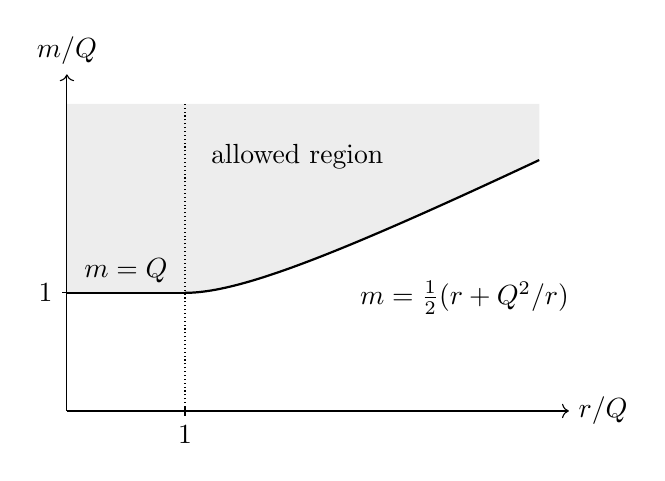
\begin{tikzpicture}[x=1.5cm,y=1.5cm]
 \fill[black!7] (0,1)--(1,1)--
   plot[domain=1:4,samples=80] (\x,{(\x+1/\x)/2})
   --(4,2.6)--(0,2.6)--cycle;
 \draw[->] (0,0)--(4.25,0) node[right] {$r/Q$};
 \draw[->] (0,0)--(0,2.85) node[above] {$m/Q$};
 \draw[thick] (0,1)--(1,1);
 \draw[thick,domain=1:4,samples=80] plot (\x,{(\x+1/\x)/2});
 \draw[densely dotted] (1,0)--(1,2.6);
 \draw (1,.04)--(1,-.04) node[below] {$1$};
 \draw (.04,1)--(-.04,1) node[left] {$1$};
 \node at (1.95,2.15) {allowed region};
 \node[below right] at (2.4,1.18) {$m=\tfrac12(r+Q^2/r)$};
 \node[above] at (.5,1) {$m=Q$};
\end{tikzpicture}
\caption{The charged upper-area inequality for $Q>0$.
For $r\le Q$, it requires only $m\ge Q$.
For $r\ge Q$, its boundary is $m=(r+Q^2/r)/2$.
The mass-lower-bound expression must therefore be restricted to this latter branch.}
\label{fig:charged-region}
\end{figure}


Two ingredients carry the charge through the neutral construction. First, we represent the fields by closed flux two-forms and keep those forms through an annular replacement, a change to a rest end, and conformal repairs. This produces strict data whose rest energies approach the original invariant mass and whose enclosing areas approach the original infimum. The quantitative repair uses only the stated weak asymptotic derivative bounds on the original data. Second, after aligning the total charge by a constant electromagnetic rotation, a pointwise square completion controls the graph norm of one closed two-form. The other rotated form has zero total charge. This single-form comparison accommodates the electromagnetic momentum density and makes the original neutral elliptic system sufficient.

The proof proceeds through four geometric stages. Section~\ref{ch:rest:section} constructs strict charged rest data. Section~\ref{ch:prep:section} prepares their exterior boundary with a positive matter margin. Sections~\ref{ch:ell:section}--\ref{ch:mass:section} use the specified neutral system to produce Riemannian comparison metrics with the same total charge, no smaller enclosing area, and a controlled energy. Section~\ref{ch:final:section} derives their Riemannian endpoint from the companion charged numerical theorem and removes the parameters in their prescribed order.

\section{Exteriors, flux forms, and conformal changes}
\label{ch:pre:section}

Throughout this part, the spatial dimension is three, $G=c=1$, and the cosmological constant is zero. Data are smooth up to every specified boundary. A subscript on a norm specifies its metric when needed. For a two-sided surface, the designated unit normal $\nu$ points into the exterior toward the chosen end, and
\[
 H=\Div_\Sigma\nu,\qquad \theta_+=H+\tr_\Sigma K.
\]
Thus outward Euclidean spheres have positive mean curvature. The spacetime convention is $K(Y,Z)=\mathbf g(\nabla_Y n,Z)$ for the future unit normal $n$.

\begin{definition}[Charged exterior]\label{ch:pre:charged-exterior}
A charged exterior consists of a connected orientable smooth three-manifold $N$ with nonempty compact smooth boundary $S$, a Riemannian metric $g$ complete with $S$ included, a symmetric covariant tensor $K$, and vector fields $\cE,\cB$. There is exactly one end. In coordinates $x$ on that end, with $r_x=|x|$, for some $q>1/2$,
\begin{equation}\label{ch:pre:falloff}
 g_{ij}-\delta_{ij}=O_2(r_x^{-q}),\quad
 K_{ij}=O_1(r_x^{-1-q}),\quad
 \cE^i,\cB^i=O_1(r_x^{-2}).
\end{equation}
The notation $O_k(r^{-b})$ bounds coordinate derivatives of order $j\le k$ by $Cr^{-b-j}$. Define the total constraint densities by
\begin{equation}\label{ch:pre:constraints}
 16\pi\mu=R_g+(\tr_gK)^2-|K|_g^2,
 \qquad
 8\pi J_i=\nabla^j\bigl(K_{ij}-(\tr_gK)g_{ij}\bigr).
\end{equation}
The functions $\mu$ and $|J|_g$ are integrable. The matter densities are
\begin{equation}\label{ch:pre:matter}
 \mu_m=\mu-\frac{|\cE|_g^2+|\cB|_g^2}{8\pi},
 \qquad
 J_m=J-\frac{(\cE\times\cB)^\flat}{4\pi},
\end{equation}
where the cross product uses the orientation and metric. They satisfy
\begin{equation}\label{ch:pre:charged-dec}
 \mu_m\ge |J_m|_g,\qquad
 \Div_g\cE=\Div_g\cB=0.
\end{equation}
The boundary satisfies $\theta_+(S)\le0$. We define ADM energy and momentum
by the following finite limits \cite{ArnowittDeserMisner1962}:
\begin{align}
 E&=\frac1{16\pi}\lim_{R\to\infty}
 \int_{|x|=R}(\partial_jg_{ij}-\partial_ig_{jj})n_\delta^i\,dA_\delta,
 \label{ch:pre:adm-energy}\\
 P_i&=\frac1{8\pi}\lim_{R\to\infty}
 \int_{|x|=R}\bigl(K_{ij}-(\tr_gK)g_{ij}\bigr)n_\delta^j\,dA_\delta,
 \label{ch:pre:adm-momentum}\\
 Q_E&=\frac1{4\pi}\lim_{R\to\infty}
 \int_{|x|=R}g(\cE,\nu_R)\,dA_g,
 \qquad
 Q_B=\frac1{4\pi}\lim_{R\to\infty}
 \int_{|x|=R}g(\cB,\nu_R)\,dA_g.
 \label{ch:pre:charges}
\end{align}
In the first two formulas the normal and area element are Euclidean; in the last two, $\nu_R$ is the outward $g$-unit normal. No extension of the physical data across $S$ is required.
\end{definition}

\subsection{Filled enclosing cuts}

A smooth enclosing cut $\Gamma$ is a compact embedded surface separating all of $S$ from the distant end. Its inner side contains the obstacle, and bounded complementary pockets are filled. Components of $\Gamma$ may coincide with components of $S$. The frontier so obtained, including any coincident part, is counted in
\begin{equation}\label{ch:pre:area-infimum}
 a_g(S)=\inf_{\Gamma}\Area_g(\Gamma).
\end{equation}
All cuts are oriented toward the end. They need not be trapped or minimal, and an individual component need not separate $S$ from infinity by itself.

\subsection{The charged bound}

\begin{theorem}\label{ch:intro:main}
Let $(N,g,K,\cE,\cB)$ be a charged exterior in the sense of Definition~\ref{ch:pre:charged-exterior}, with inner boundary $S$, ADM energy and momentum $(E,P)$, and total charges $(Q_E,Q_B)$. Then $E>|P|$. Setting
\[
 m=\sqrt{E^2-|P|^2},\qquad
 Q=\sqrt{Q_E^2+Q_B^2},\qquad
 r=\sqrt{a_g(S)/(4\pi)},
\]
we have
\[
 m\ge Q,\qquad r\le m+\sqrt{m^2-Q^2}.
\]
\end{theorem}

Here $a_g(S)$ is the minimum enclosing area, defined as an infimum over all smooth filled enclosing cuts. Neither the inner boundary nor a competing cut is required to be connected. The boundary condition is only $H+\tr_S K\le0$, with the normal pointing toward infinity. The electromagnetic fields are divergence free, and the remaining matter satisfies the dominant energy condition. The statement places no maximality, symmetry, or zero-momentum restriction on the initial data.

\begin{lemma}\label{ch:pre:area-positive}
For every exterior as above, $0<a_g(S)<\infty$. If the infimum is instead defined using filled finite-perimeter inner sets that retain the obstacle and count its coincident frontier, its value is unchanged.
\end{lemma}

\begin{proof}
After forgetting $K$ and the fields, Definition~\ref{ch:pre:charged-exterior}
gives an exterior in Definition~\ref{n3:intro:exterior-class}, with the
same boundary $S$. Lemma~\ref{bridge:bridge:positive-area} therefore gives
$0<a_g(S)<\infty$.

For the perimeter assertion, apply
Lemma~\ref{n3:reduction:area-compactness} to the constant sequence $g_j=g$.
Local convergence is immediate. The falloff in
Equation~\eqref{ch:pre:falloff} gives uniform end bounds
$c\delta\le g\le C\delta$ and $r_x|\partial g|\le C$, and a fixed
large coordinate sphere is a compact enclosing competitor of finite
area. The lemma consequently identifies the smooth and perimeter
infima. Its competitors are the same bounded filled inner sets used here:
they retain the entire obstacle, bounded complementary pockets are
filled, and the full frontier, including contact with $S$, is counted.
Its outward smoothing preserves enclosure and proves the claimed
equality of infima. The auxiliary filling in that perimeter argument
requires no extension of the physical data or energy condition.
\end{proof}

\subsection{The neutral exterior inequality in this notation}

We first record the form of Theorem~\ref{n3:intro:exterior-inequality} used below. The transfer retains arbitrary compact boundary topology and a potentially disconnected boundary.

\begin{proposition}[Neutral exterior inequality]
\label{ch:pre:neutral-exterior}
Let $(N,g,K)$ be a smooth connected orientable one-ended exterior, complete with its nonempty compact smooth boundary $S$ included. Suppose the metric and tensor satisfy the first two bounds in \eqref{ch:pre:falloff}, the densities \eqref{ch:pre:constraints} are integrable as above, the ADM limits \eqref{ch:pre:adm-energy}--\eqref{ch:pre:adm-momentum} are finite, and $\mu\ge|J|_g$ throughout $N$. If $H+\tr_SK\le0$ and $E>|P|$, then
\[
 \sqrt{E^2-|P|^2}\ge\sqrt{a_g(S)/(16\pi)}.
\]
No complete fill-in across $S$ is part of the hypothesis.
\end{proposition}

\begin{proof}
Apply Theorem~\ref{n3:intro:exterior-inequality} with its exterior
$\Omega=N$. Definition~\ref{ch:pre:charged-exterior}, after the field
requirements are omitted, uses the same smoothness, orientation,
one-endedness and completeness convention as
Definition~\ref{n3:intro:exterior-class}. Equations~\eqref{ch:pre:constraints},
\eqref{ch:pre:adm-energy} and~\eqref{ch:pre:adm-momentum} are exactly its
constraint and ADM conventions. The decay, integrability, weak expansion
and future timelike hypotheses in the proposition are precisely those
of that theorem. The class of filled enclosing cuts is also identical:
all boundary components are enclosed, bounded pockets are filled, and
coincident obstacle frontier is counted. Hence its enclosing infimum is
$a_g(S)$, giving the displayed inequality. The theorem is one-sided and
requires no extension across $S$.
\end{proof}

\subsection{Flux forms and a conformal inequality}

Put $X_1=\cE$, $X_2=\cB$, and
\begin{equation}\label{ch:pre:flux-forms}
 \alpha_i=\iota_{X_i}dV_g.
\end{equation}
The divergence equations are $d\alpha_i=0$. Their fluxes across every filled enclosing cut are $4\pi Q_E$ and $4\pi Q_B$. In every change of metric below, retaining a flux form means defining its new vector field by contraction with the new volume form. This preserves closedness and all fluxes without choosing a vector potential.

For $|Y|_g\le1$, define
\begin{align}
 I_g(Y)&=|X_1|_g^2+|X_2|_g^2
       +2\langle X_1\times X_2,Y\rangle_g,
 \label{ch:pre:I}\\
 D_g(Y)&=8\pi\bigl(\mu+J(Y)\bigr)-I_g(Y).
 \label{ch:pre:D}
\end{align}
Then
\begin{equation}\label{ch:pre:margin}
 I_g(Y)\ge0,\qquad
 \inf_{|Y|_g\le1}D_g(Y)
 =8\pi(\mu_m-|J_m|_g)=:M_0.
\end{equation}
The first assertion uses $2|X_1\times X_2|\le|X_1|^2+|X_2|^2$. The second follows by minimizing the linear term $8\pi J_m(Y)$ over the unit ball. Both $I_g$ and $D_g$ are invariant under a constant $SO(2)$ rotation of the pair of forms. The same elementary inequality and the triangle inequality imply
\begin{equation}\label{ch:pre:neutral-margin}
 8\pi(\mu-|J|_g)\ge M_0.
\end{equation}

\begin{lemma}[Conformal charged comparison]\label{ch:pre:conformal}
Let $u\ge1$ be smooth, and set $g'=u^4g$, $K'=u^2K$, retaining the two flux forms. For every $|Y|_g\le1$,
\begin{equation}\label{ch:pre:conformal-estimate}
 u^4D_{g'}(u^{-2}Y)
 \ge D_g(Y)+4u^{-1}\bigl(-\Delta_gu-|K|_g|du|_g\bigr).
\end{equation}
At a fixed oriented surface,
\begin{equation}\label{ch:pre:conformal-boundary}
 \theta_+'=u^{-2}\bigl(\theta_++4\partial_\nu\log u\bigr).
\end{equation}
Here $\Delta_g=\Div_g\nabla$.
\end{lemma}

\begin{proof}
The conformal scalar-curvature formula and the scaling of the tensor terms in \eqref{ch:pre:constraints} give
\[
 16\pi u^4\mu'=16\pi\mu-8u^{-1}\Delta_gu.
\]
For $f=\log u$, the difference of the two connections is
\[
 \nabla'_AB-\nabla_AB
 =2\bigl(df(A)B+df(B)A-g(A,B)\nabla f\bigr).
\]
Taking the divergence of the rescaled trace reversal
$u^2(K-(\tr_gK)g)$ therefore yields
\[
 8\pi u^2J'=8\pi J+4K(\nabla\log u,\cdot).
\]
The new field vectors are $X_i'=u^{-6}X_i$, so their components in orthonormal frames scale by $u^{-4}$ and
$I_{g'}(u^{-2}Y)=u^{-8}I_g(Y)$. Consequently
\[
 u^4D_{g'}(u^{-2}Y)
 =D_g(Y)+(1-u^{-4})I_g(Y)
 +4u^{-1}\bigl(-\Delta_gu+K(\nabla u,Y)\bigr).
\]
Dropping the nonnegative second term and estimating the last tensor contraction proves \eqref{ch:pre:conformal-estimate}. Finally,
$H'=u^{-2}(H+4\partial_\nu\log u)$ and
$\tr_\Sigma^{g'}K'=u^{-2}\tr_\Sigma^gK$, which give \eqref{ch:pre:conformal-boundary}.
\end{proof}

\section{Charge-preserving reduction to strict rest data}
\label{ch:rest:section}

Throughout this section the closed forms $\alpha_1,\alpha_2$ are fixed.
For each new metric they define new electromagnetic vector fields by
contraction with its volume form. Thus every change below preserves both
Maxwell constraints and both signed charges. We first apply the
neutral endpoint corollary to establish timelikeness of the original data.

\begin{proposition}[Strict rest reduction]
\label{ch:rest:reduction}
For a charged exterior as in Definition~\ref{ch:pre:charged-exterior}, $E>|P|$ and
$m=(E^2-|P|^2)^{1/2}>0$. There are smooth data $(g_j,K_j)$ on the same
exterior, with the same flux forms, satisfying the following properties.
\begin{enumerate}
\item The physical matter condition is strict everywhere, the original
boundary $S$ has $\theta_{+,j}<0$, and the constraint densities remain
integrable. For one fixed $0<\delta<1$ the matter margin satisfies
\[
 M_{0,j}=8\pi(\mu_{m,j}-|J_{m,j}|_{g_j})
       \ge c_j r_y^{-3-\delta}\quad\hbox{far out},\qquad c_j>0.
\]
\item In a rest chart $y$, $K_j$ is compactly supported and
\[
 g_j-\delta_{\mathrm{eucl}}=O_k(r_y^{-1}),\qquad
 R_{g_j}=O_k(r_y^{-3-\delta})\quad\hbox{for every }k.
\]
The fields have the required $O_1(r_y^{-2})$ decay. In particular the
ADM momentum is zero and $\Ric_{g_j}=O(r_y^{-3})$.
\item Smooth convergence holds on every compact set, including at $S$,
and
\begin{equation}
 \label{ch:rest:limits}
 E_j\longrightarrow m,\qquad
 a_{g_j}(S)\longrightarrow a_g(S),\qquad
 (Q_{E,j},Q_{B,j})=(Q_E,Q_B).
\end{equation}
Moreover $g_j\ge(1-\varepsilon_j)g$ globally for some
$\varepsilon_j\downarrow0$.
\end{enumerate}
\end{proposition}

The proof has four steps: establish timelikeness from the neutral
endpoint corollary; replace the distant end by a vacuum reference with
matching ADM vector; bend and repair while retaining the flux forms;
and make the inequalities strict by a separate elliptic construction.
All quantitative estimates for the replacement use exactly the original
$O_2$ metric and $O_1$ tensor assumptions.

\subsection{Timelikeness}

\begin{lemma}
\label{ch:rest:timelike}
The original ADM vector satisfies $E>|P|$.
\end{lemma}
\begin{proof}
The physical matter condition and Equation~\eqref{ch:pre:neutral-margin}
give
\[
 \mu-|J|_g\ge\mu_m-|J_m|_g\ge0.
\]
These are the actual total constraint densities of $(g,K)$.
Definition~\ref{ch:pre:charged-exterior} supplies smoothness, orientation,
one-endedness, completeness with the nonempty compact boundary included,
the required metric and tensor falloff, integrable total densities,
finite ADM limits, and weak future trapping with the normal toward the
end. The total constraint and ADM conventions are exactly those of
Equations~\eqref{n3:intro:constraints}, \eqref{n3:intro:energy} and
\eqref{n3:intro:momentum}. All hypotheses of
Corollary~\ref{bridge:bridge:timelike} are therefore satisfied.
Applying it to the unchanged data $(N,g,K)$ yields $E>|P|$
for their original ADM vector.
\end{proof}

\subsection{A matching vacuum reference and annular replacement}

\begin{lemma}[Boosted vacuum reference]
\label{ch:rest:reference}
There is an auxiliary Schwarzschild end of mass $m$ whose induced data
$(g_*,K_*)$, in asymptotically Euclidean coordinates $x$, have ADM vector
$(E,P)$ and satisfy
$g_*-\delta_{\mathrm{eucl}}=O_k(r_x^{-1})$,
$K_*=O_k(r_x^{-2})$ for every $k$.
\end{lemma}
\begin{proof}
Lemma~\ref{ch:rest:timelike} gives $E>|P|$. The constraint and ADM
conventions in Equations~\eqref{ch:pre:constraints},
\eqref{ch:pre:adm-energy}, and~\eqref{ch:pre:adm-momentum} agree with
those in Part~I. Lemma~\ref{n3:reduction:boosted-reference} therefore
gives the required reference end, including the stated differentiated
decay and the future second-form convention.

For the later bend, retain its static isotropic coordinates:
\begin{equation}
 \label{ch:rest:schwarzschild}
 \mathbf g=-\left(\frac{1-m/(2r_y)}{1+m/(2r_y)}\right)^2dT^2
       +\left(1+\frac m{2r_y}\right)^4|dy|^2.
\end{equation}
The reference plane is $T=v\cdot y$, with $|v|<1$ chosen to give
$(E,P)$. Its asymptotically Euclidean coordinates are $y=Ax$, where
$A=(I-vv^\top)^{-1/2}$, since $A^\top(I-vv^\top)A=I$.
\end{proof}

For the remaining construction, fix $1/2<\beta<\min(q,1)$.

\begin{lemma}[Annular replacement]
\label{ch:rest:annular}
For sufficiently large $R$ there are smooth data equal to $(g,K)$ on
$r_x\le R$ and to $(g_*,K_*)$ on $r_x\ge4R$, with possible neutral
DEC deficit bounded by $\eta_R R^{-3}$ in between, where
$\eta_R\to0$. The estimates use no derivatives beyond the assumed
two metric derivatives and one tensor derivative.
\end{lemma}
\begin{proof}
The original data satisfy neutral DEC by
Equation~\eqref{ch:pre:neutral-margin}. Definition~\ref{ch:pre:charged-exterior}
gives the smooth one-ended exterior, completeness with its compact
boundary included, decay $g-\delta=O_2(r_x^{-q})$ and
$K=O_1(r_x^{-1-q})$ with $q>1/2$, integrable total constraint
densities, and finite ADM limits. The total constraint and ADM
normalizations agree with those used in
Proposition~\ref{n3:reduction:annular-replacement}.
The reference in Lemma~\ref{ch:rest:reference} has matching charges
in the common $x$ coordinates, and $E>|P|$ by
Lemma~\ref{ch:rest:timelike}. That proposition applies and gives
\[
 16\pi(\widetilde\mu_R-
       |\widetilde J_R|_{\widetilde g_R})
 \ge -\eta_RR^{-3},\qquad \eta_R\longrightarrow0,
\]
with the stated exact agreement on both sides of the annulus and
with quantitative estimates using only the original two metric
derivatives and one tensor derivative. Absorbing the fixed
normalization into $\eta_R$ gives the assertion.
The scaled construction in Equation~\eqref{n3:reduction:scaled-smallness}
and the compact corrections in that proposition's proof also give
\[
 \|\widetilde g_R(R\,\cdot)-I\|_{C^2(\{1<|z|<4\})}
 +\|R\widetilde K_R(R\,\cdot)\|_{C^1(\{1<|z|<4\})}
 \le C R^{-\beta}.
\]
The two closed flux forms are retained throughout; their contribution
to the physical matter deficit is estimated next.
\end{proof}

\subsection{Bending and repairing the physical matter condition}

Beyond the annular replacement, use the exact Schwarzschild part and
replace the plane by the graph
\begin{equation}
 \label{ch:rest:bend}
 T_R(y)=(v\cdot y)\psi\left(\frac{\log(r_y/R_b)}{L_0}\right).
\end{equation}
Here $\psi$ is smooth, is one before zero and zero after one, and takes
values in $[0,1]$. The fixed multiple $R_b/R$ is large enough that the
bend begins beyond $r_x=4R$. First fix $L_0$ so large that
$|v|(1+\|\psi'\|_\infty/L_0)<1$. Then the graph is uniformly
spacelike: in Equation~\eqref{ch:rest:schwarzschild} the spatial factor
is greater than one and the lapse is less than one. Its constraints
vanish by Gauss--Codazzi with the prescribed future normal.

Write $(g_R,K_R)$ for the unscaled replacement and bend. Constants in
the rest of this subsection may depend on the fixed original data and
$L_0$, but not on $R$. The graph formula and its first three derivatives
give uniform metric comparability, $|\partial g_R|+|K_R|\le C/r_y$ in
the transition, and
\begin{equation}
 \label{ch:rest:radial-geometry}
 c\le|dr_y|_{g_R}\le C,\qquad
 |\Delta_{g_R}r_y|\le C/r_y.
\end{equation}
The same bounds hold on the gluing annulus, since $y=Ax$ is a fixed
linear map. Outside a fixed multiple of $R$, the data are horizontal
Schwarzschild and $K_R=0$.

Keep the original closed forms in these coordinates. Their norms are
$O(r_y^{-2})$, so their contribution to the negative part of
$\inf_{|Y|\le1}D_{g_R}(Y)$ is $O(r_y^{-4})$. Choose fixed
$0<a<\xi_0<b$ so that the data are original for $r_y/R\le\xi_0$
and horizontal Schwarzschild for $r_y/R\ge b$.
Lemma~\ref{ch:rest:annular} and vacuum of the reference and bend imply
\begin{equation}
 \label{ch:rest:charged-deficit}
 \bigl[-\inf_{|Y|_{g_R}\le1}D_{g_R}(Y)\bigr]_+
 \le
 \begin{cases}
 0,& r_y/R\le\xi_0,\\
 \eta_R R^{-3},&\xi_0\le r_y/R\le b,\\
 Cr_y^{-4},&r_y/R\ge b,
 \end{cases}
 \qquad\eta_R\longrightarrow0.
\end{equation}
Thus this intermediate data set is not assumed to satisfy charged DEC.

\begin{lemma}[Charged repair with vanishing energy cost]
\label{ch:rest:charged-repair}
There are smooth $u_R\ge1$, constant on the unchanged core, for which
$(u_R^4g_R,u_R^2K_R)$ with the fixed forms satisfy the physical matter
condition. They retain weak trapping, have zero ADM momentum, and their
energies tend to $m$. Moreover $\|u_R-1\|_\infty=o(R^{-1})$, and
the final metric has all-order $O(r_y^{-1})$ asymptotics and
scalar curvature $R_{u_R^4g_R}=O_k(r_y^{-4})$.
\end{lemma}
\begin{proof}
Set $\xi=r_y/R$ and seek
\[
 u_R=1+\frac{e_R}{R}F_R(\xi),\qquad
 F_R(\xi)=\int_\xi^\infty z_R(t)\,dt,
 \qquad z_R\ge0,
\]
where $e_R\to0$ will be chosen below. On $[a,b+1]$ initially solve
$z_R'=C_0z_R+\omega$, $z_R(a)=0$, where $\omega\ge0$ is smooth,
zero near $a$, and at least one on $[\xi_0,b+1]$; extend $z_R=0$
below $a$. Equation~\eqref{ch:rest:radial-geometry} yields
\begin{align}
 -\Delta_{g_R}u_R-|K_R|_{g_R}|du_R|_{g_R}
 &=\frac{e_R}{R^3}
  \{z_R'|dr_y|^2+Rz_R\Delta r_y-Rz_R|K_R||dr_y|\}\notag\\
 &\ge\frac{e_R}{R^3}(c z_R'-Cz_R).
 \label{ch:rest:repair-inequality}
\end{align}
Choose $C_0$ large. This is nonnegative on $[a,b]$ and at least
$c'e_R R^{-3}$ on $[\xi_0,b]$.

On the horizontal region put
$A_R(t)=(t+m/(2R))^2z_R(t)$. Its derivative from the preceding
prescription is positive near $b$. Continue that derivative smoothly
by a convex blend with $t^{-2}$ over $[b,b+1]$, and integrate from
$A_R(b)$. Thus $A_R'\ge c''t^{-2}$ for $t\ge b$ and
$A_R'=t^{-2}$ eventually. Defining
$z_R=A_R(t)/(t+m/(2R))^2$ there makes every join smooth. For fixed
$L_0$, $A_R^\infty=\lim_{t\to\infty}A_R(t)$ and $F_R$ are bounded
uniformly in $R$. The exact radial Laplacian on the horizontal slice is
\begin{equation}
 \label{ch:rest:tail-repair}
 -\Delta_{g_R}u_R
 =\frac{e_R}{R^3}
   \left(1+\frac m{2R\xi}\right)^{-6}\xi^{-2}A_R'(\xi)
 \ge c'''e_R R^{-3}\xi^{-4}.
\end{equation}
Choose, for example, $e_R=C_1(\eta_R+R^{-1})$, with a sufficiently
large fixed $C_1$. For large $R$, $1\le u_R\le2$.
Equations~\eqref{ch:rest:repair-inequality}--\eqref{ch:rest:tail-repair}
then dominate $u_R/4$ times the deficit in
Equation~\eqref{ch:rest:charged-deficit}.
Equation~\eqref{ch:pre:conformal-estimate} proves the physical matter condition.
The factor is constant near $S$, so
Equation~\eqref{ch:pre:conformal-boundary} preserves its weak expansion.

At infinity, for each fixed $R$,
\[
 u_R=1+\frac{e_RA_R^\infty}{r_y}+O_k(r_y^{-2})
 \quad\hbox{for every }k.
\]
The ADM energy is therefore $m+2e_RA_R^\infty\to m$ and the momentum
vanishes because $K_R$ has compact support. The differentiated radial
formula gives scalar curvature $O_k(r_y^{-4})$. This also verifies
integrability of the repaired constraints. Completeness follows from
the comparability of the intermediate metric and $u_R\ge1$.
\end{proof}

\subsection{Strictification by an exterior elliptic problem}

\begin{lemma}[A strict conformal direction]
\label{ch:rest:strict-direction}
Fix one repaired exterior $(g_0,K_0)$ from
Lemma~\ref{ch:rest:charged-repair}, and fix $0<\delta<1$. There exist
smooth positive $w_0,\phi_0$ such that
\begin{equation}
 \label{ch:rest:strict-direction-equations}
 \partial_\nu\phi_0=-1\text{ on }S,\qquad
 -\Delta_{g_0}\phi_0-|K_0|_{g_0}|d\phi_0|_{g_0}\ge w_0,
\end{equation}
where $w_0=r_y^{-3-\delta}$ and
$-\Delta_{g_0}\phi_0=w_0$ far out, and
$\phi_0=O_k(r_y^{-1})$ for every $k$.
Its gradient has finite flux at infinity. All constants in this lemma
may depend on the fixed repaired exterior.
\end{lemma}
\begin{proof}
Choose a smooth nonnegative compactly supported majorant
$b_0\ge|K_0|_{g_0}$ and a smooth positive extension $w_0$ of the
specified tail. We solve the regularized equation
\begin{equation}
 \label{ch:rest:semilinear}
 -\Delta_{g_0}\phi=b_0\sqrt{1+|d\phi|_{g_0}^2}+w_0,
 \qquad\partial_\nu\phi=-1,\qquad\phi\longrightarrow0.
\end{equation}
First truncate at $r_y=T$ and impose outer Dirichlet value zero.
Multiply $b_0$ by $t\in[0,1]$ for continuation. At $t=0$ the mixed
Laplacian is invertible, by the Dirichlet Poincar\'e inequality and
elliptic regularity. Every linearization is a uniformly elliptic
Laplacian with drift of norm at most $b_0$, with homogeneous Neumann
data on $S$ and Dirichlet data on the outer sphere. These faces are
disjoint. The maximum and Hopf principles give zero kernel; as a
compact lower-order perturbation of the mixed Laplacian, it is
Fredholm of index zero and is invertible.

We supply the estimates needed for closedness. On this fixed truncation,
the $W^{2,p}$ estimate and gradient interpolation give, uniformly in $t$,
\[
 \|\phi\|_{W^{2,p}}
 \le C(1+\|\phi\|_{L^p}+\|d\phi\|_{L^p})
 \le\tfrac12\|\phi\|_{W^{2,p}}+C'(1+\|\phi\|_\infty).
\]
If the supremum norms were unbounded, divide by them and take $p>3$.
A subsequence converges in $C^1$ to a nonzero solution $v$ with
homogeneous mixed data and
$-\Delta_{g_0}v=t_*b_0|dv|$. Indeed the normalized right side is
$t b_0\sqrt{M^{-2}+|dv|^2}+w_0/M$ when $M=\|\phi\|_\infty$.
The limit is a homogeneous bounded-drift equation, taking drift
$t_*b_0\nabla v/|dv|$ off the critical set and zero on it. The strong
and Hopf maximum principles exclude such a nonzero $v$.
The resulting supremum and $W^{2,p}$ bounds, followed by Schauder
estimates for the smooth regularized equation, close continuation.
Thus every sufficiently large truncation has a smooth solution.

All solutions are nonnegative: a negative minimum cannot be interior
since the source is positive, or on $S$ since the outward-domain
derivative there is $-\partial_\nu\phi=1$, contradicting the Hopf
sign at a minimum. Fix a core containing $\supp b_0$. On its exterior
$f=r_y^{-1}-r_y^{-1-\delta}$ is positive and
\[
 -\Delta_{g_0}f
 =\delta(1+\delta)r_y^{-3-\delta}+O(r_y^{-4})
 \ge c w_0
\]
after enlarging the fixed core. Comparison with a multiple of $f$
gives, independently of $T$,
\begin{equation}
 \label{ch:rest:core-barrier}
 0\le\phi\le C(1+M_T)r_y^{-1}\quad\hbox{outside the core},
 \qquad M_T=\sup_{\mathrm{core}}\phi.
\end{equation}
If $M_T\to\infty$ along an exhaustion, divide by $M_T$. Local
$W^{2,p}$ estimates, including the fixed inner Neumann boundary,
and Equation~\eqref{ch:rest:core-barrier} give a limit $v\ge0$ with
maximum one on the core, homogeneous inner Neumann condition,
$-\Delta v=b_0|dv|$, and $v\to0$ at infinity. Its positive global
maximum is attained, contradicting the strong or Hopf principle.
Hence the core bounds are uniform in $T$. Diagonal compactness and
bootstrap give a smooth global solution of
Equation~\eqref{ch:rest:semilinear}, positive also on $S$ by the same
minimum argument.

On the end its equation is the linear Poisson equation
$-\Delta_{g_0}\phi_0=w_0$. On a scaled annulus the function
$\rho\phi_0(\rho\,\cdot)$ is uniformly bounded; the scaled metric
has all-order bounds and the scaled source is $O(\rho^{-\delta})$
with all its derivatives. Interior Poisson estimates of each order
therefore give $\phi_0=O_k(r_y^{-1})$. The full right side of
Equation~\eqref{ch:rest:semilinear} is integrable. The divergence theorem
then gives a finite metric gradient flux, and its difference from the
Euclidean flux is $O(r_y^{-1})$. This proves every assertion.
\end{proof}

For $u=1+s\phi_0$, $s>0$, use $(u^4g_0,u^2K_0)$ and the fixed
forms. Equations~\eqref{ch:pre:conformal-estimate} and
\eqref{ch:rest:strict-direction-equations} imply
\begin{equation}
 \label{ch:rest:strict-margin}
 M_{0,s}\ge4s u^{-5}w_0>0,
 \qquad
 \theta_{+,s}=u^{-2}(\theta_{+,0}-4s/u)<0\quad\hbox{on }S.
\end{equation}
Compact support of $K_0$ persists. The conformal scalar formula gives
the asserted all-order $r_y^{-3-\delta}$ scalar decay, and thus
integrability. The ADM energy change is
\begin{equation}
 \label{ch:rest:strict-energy}
 E_s-E_0=-\frac{s}{2\pi}
   \lim_{r\to\infty}\int_{r_y=r}\partial_{\nu_r}\phi_0\,dA_{g_0}
   =O(s).
\end{equation}
The metric and Euclidean fluxes agree in this formula by the estimates
just proved. For the fixed repaired datum the finite coefficient and
any finite collection of compact smooth norms can be made arbitrarily
small by choosing $s$ small; no bound uniform in the bending radius is
needed.

\subsection{Global area control and the diagonal limit}

\begin{proof}[Completion of the proof of Proposition~\ref{ch:rest:reduction}]
It remains to check area and organize the parameters. On the vacuum
plane and bend, write $dT_R=\psi a+b$, where $a=v\cdot dy$ and
$|b|\le C L_0^{-1}|dy|$. Since $0\le\psi\le1$,
$dT_R^2\le a^2+C L_0^{-1}|dy|^2$ as quadratic forms. The spatial
factor and lapse in Equation~\eqref{ch:rest:schwarzschild} consequently
give
\begin{equation}
 \label{ch:rest:global-lower-comparison}
 g_R\ge |dy|^2-dT_R^2
 \ge|dy|^2-(v\cdot dy)^2-\frac C{L_0}|dy|^2
 \ge\left(1-\frac{C'}{L_0}\right)|dx|^2.
\end{equation}
The constants here depend on the fixed boost, not on $R$ or large
$L_0$. In the gluing annulus $g_R=I+O(R^{-\beta})$, whereas the
original metric is uniformly $I+o(1)$ throughout the receding end.
On the unchanged core the metrics agree. Both conformal changes
increase the metric. Thus first choosing $L_0\to\infty$ and then
$R\to\infty$ sufficiently fast gives the global comparison
$g_j\ge(1-\varepsilon_j)g$ with $\varepsilon_j\to0$.

For each fixed $L_0$ the energy of the repaired data tends to $m$ by
Lemma~\ref{ch:rest:charged-repair}. Select $R$ to make this energy error,
the constant core conformal change, and the preceding comparison error
arbitrarily small. Finally choose the strictification parameter $s_j$
to make Equation~\eqref{ch:rest:strict-energy} tend to zero and to control
the first $j$ smooth norms on the first $j$ sets of a compact exhaustion.
This gives local smooth convergence and all the analytic assertions of
the proposition. Each metric is complete up to $S$, by the global
positive comparison and smoothness. The fixed linear relation $y=Ax$
and the all-order metric asymptotics preserve the $O_1(r_y^{-2})$
field bounds, since the forms themselves are fixed.

For every smooth filled enclosing cut $\Gamma$, the quadratic-form
comparison gives
\[
 \Area_{g_j}(\Gamma)\ge(1-\varepsilon_j)\Area_g(\Gamma).
\]
Hence $\liminf_j a_{g_j}(S)\ge a_g(S)$. Conversely fix any such cut
with area within $\zeta>0$ of $a_g(S)$. Local convergence on this
compact cut gives
$\limsup_j a_{g_j}(S)\le\Area_g(\Gamma)\le a_g(S)+\zeta$;
let $\zeta\downarrow0$. This proves the area limit directly for the
smooth-cut infimum, including obstacle-coincident components.
Finally each enclosing cut has the same flux of each fixed closed
form by Stokes' Theorem, so both charges are preserved exactly.
\end{proof}

The proposition constructs charged initial data on the original exterior
and recovers its invariant mass;
it does not assert that the original data admit a spacetime embedding
or a global Lorentz change of asymptotic slice.

\section{Geometric preparation with the physical matter margin}
\label{ch:prep:section}

Fix a strict rest datum from Proposition~\ref{ch:rest:reduction}, denoted
by $(N,g,K,\alpha_1,\alpha_2)$, with obstacle $S_0$, energy $E_*>0$,
and $A_*=a_g(S_0)$. Retain its geometry and end estimates; in
particular, $K$ has compact support and $\theta_+(S_0)<0$.
Its physical and neutral margins satisfy
\begin{equation}\label{ch:prep:margin}
 M_0=8\pi(\mu_m-|J_m|_g)>0,
 \qquad 8\pi(\mu-|J|_g)\geq M_0,
 \qquad M_0\geq c_*r_y^{-3-\delta_*}
 \quad\text{far out},
\end{equation}
where $c_*>0$ and $0<\delta_*<1$ are fixed for this datum.
Every choice and constant in this section concerns this fixed datum.

\subsection{The bounding regions and their orientations}

For a symmetric tensor $T$ write
$\Theta_T(\Sigma,\nu)=H_\Sigma(\nu)+\tr_\Sigma T$.
The geometric input is the following form of the three-dimensional
barrier and total trapped-region theorems
\cite[Section~2, Theorems~3.1 and~4.1, Definitions~7.1--7.2,
and Theorem~7.3]{AnderssonMetzger2009}.

\begin{theorem}[Barrier and total trapped-region theorem]
\label{ch:prep:region-theorem}
Let $(D,g,T)$ be smooth compact connected three-dimensional data with boundary
$\Gamma_-\sqcup\Gamma_+$.  Assume $\Gamma_+\ne\varnothing$ and
$\Theta_T(\Gamma_+)>0$ with its normal out of $D$.  The inner boundary
may be empty; when present it satisfies $\Theta_T(\Gamma_-)<0$ with
its normal into $D$.  All boundary parts may be disconnected.

Consider all smooth bounding domains containing a relative collar
of $\Gamma_-$, avoiding $\Gamma_+$, and having interior free boundary
with $\Theta_T\leq0$ for the normal out of the bounding domain.
If the union is nonempty, its closure is a maximal
closed bounding region whose interior frontier is smooth, compact,
embedded, stable, and satisfies $\Theta_T=0$.  It is itself the
closure of an admissible domain.  A nonempty strict inner barrier
ensures a nonempty union and an enclosing stable MOTS.
No energy condition or constraint equation is required for $T$.
\end{theorem}

Filling a complementary component incident on no designated outer
boundary deletes whole free-boundary components and preserves the
expansion of those retained.  This filling convention is understood
in Theorem~\ref{ch:prep:region-theorem} and throughout the construction.
Two identities fix the shifted tensors and all orientations:
\begin{equation}\label{ch:prep:shift-reversal}
 \Theta_{T-(c/2)g}=\Theta_T-c,
 \qquad \Theta_{-T}(\Sigma,-\nu)=-\Theta_T(\Sigma,\nu).
\end{equation}

Choose $R_0$ beyond $\supp K$ so that every coordinate sphere of
radius at least $R_0$ has positive outward mean curvature.  Every
compact bounding domain with $\Theta_{\pm K}\leq c\leq0$ is confined
inside this fixed radial range.  Indeed, at a free-boundary point
of maximum radius beyond $R_0$, the boundary lies inside the tangent
coordinate sphere with the same outward normal.  The local graph
comparison gives $H_{\partial D}\geq H_{S_r}>0$, whereas $K=0$.
This contradicts the expansion bound.  Consequently all families
below can be constructed on a single compact truncation, independently
of the sufficiently distant outer sphere.

For $\max_{S_0}\Theta_K(S_0)<c<0$, let $\mathcal B_c$ be the
\emph{full} closed maximal region for $\Theta_K\leq c$, with $S_0$
as required inner boundary.  Applying
Theorem~\ref{ch:prep:region-theorem} to $K-(c/2)g$ is legitimate:
$S_0$ is strictly negative and the distant sphere strictly positive
for the shifted expansion.  Thus $\mathcal B_c$ is nonempty, contains
a collar of $S_0$, and has smooth stable frontier at expansion $c$.
These regions increase with $c$.

Fix such a threshold $c_b$ and put $\mathcal B=\mathcal B_{c_b}$.
In its filled complement, designate both the full black frontier and a
distant sphere as \emph{outer} barriers.  There is no required inner
boundary.  For $c<0$, let $\mathcal W_c$ be the full closed maximal
region of compact bounding domains satisfying $\Theta_{-K}\leq c$
there.  On the reversed black frontier the expansion of
$-K-(c/2)g$ equals $-c_b-c>0$; it is positive on the distant
sphere as well.  Theorem~\ref{ch:prep:region-theorem} therefore applies
whenever the union is nonempty.  Its smooth stable frontier has
$\Theta_{-K}=c$ and positive separation from the black frontier.
If the union is empty, set $\mathcal W_c=\varnothing$.  The white
family increases with $c$, always with the black region held fixed.

We choose the two thresholds successively at points of Hausdorff
right continuity of these full families.  Here is the elementary
selection argument, including emptiness.  For any increasing closed
family $E_c$ in a compact metric space, choose a cap $L$ larger than
its diameter and put
$d_c(x)=\min\{L,\dist(x,E_c)\}$, taking $d_c\equiv L$ if
$E_c=\varnothing$.  At every point of a countable dense set, this
is a bounded nonincreasing function of $c$ and has at most countably
many right discontinuities.  Avoid their union.  The common
$1$-Lipschitz bound and a finite-net argument then give uniform
convergence $d_{c_j}\to d_c$ whenever $c_j\downarrow c$.  For
nonempty $E_c$ this gives Hausdorff convergence, since
$E_c\subset E_{c_j}$.  For empty $E_c$, uniform convergence to $L$
forces every sufficiently close $E_{c'}$, $c'>c$, to be empty:
otherwise its distance function has a zero.  Thus $c_b$, and then
$c_w$ for this fixed $\mathcal B$, can be chosen arbitrarily close
to zero with the stated continuity, including the empty-white case.

Put $\mathcal W=\mathcal W_{c_w}$ and let $X$ be the closure of the
component toward infinity of $N\setminus(\mathcal B\cup\mathcal W)$.
Its boundary is the entire adjacent frontier, a finite disjoint
union $B=B_b\sqcup B_w$ of complete black and white face components.
It is nonempty because the excluded side contains $S_0$ and its
collar.  Both full frontiers are compact and disjoint, so selection
creates no corners.  With $\nu$ pointing into $X$, set
$H=H_B(\nu)$ and $P_B=\tr_BK$.  Then
\begin{equation}\label{ch:prep:faces}
 H+P_B=c_b\quad\text{on }B_b,
 \qquad H-P_B=c_w\quad\text{on }B_w.
\end{equation}
Either face type may be absent from $B$; for example a white face
can separate a black face from infinity.  The full regions used to
choose the thresholds are retained in the preparation even when
some of their frontier components are not adjacent to $X$.

The restricted data on $X$ are smooth and complete up to $B$, with
the original single end.  Every enclosing cut $\Gamma$ for $B$ is
also a cut for $S_0$ after the discarded side is adjoined to its
inner region and bounded pockets are filled.  Therefore
\begin{equation}\label{ch:prep:enclosure}
 \Area_g(\Gamma)\geq A_*,
 \qquad
 \frac1{4\pi}\int_\Gamma\alpha_i
   =\frac1{4\pi}\int_B\alpha_i=Q_i\quad(i=1,2),
 \qquad (Q_1,Q_2)=(Q_E,Q_B).
\end{equation}
The flux equalities follow from closedness and Stokes' Theorem
between the cut and a distant sphere, all normals pointing toward
the end.  These assertions concern the whole frontier and do not
require any individual component to separate $S_0$ from infinity.

\subsection{Stable collars and a stronger offset bound}

\begin{lemma}[Outward leaf collars]\label{ch:prep:collar}
Each connected face has a smooth outward collar with leaf parameter
$s\geq0$, $s=0$ on the face, and $|\nabla s|$ bounded above and
below by positive constants.  Its leaves satisfy
$\Theta_K>c_b$ for black faces and $\Theta_{-K}>c_w$ for white
faces whenever $s>0$.  The collars may be chosen disjoint in $X$.
\end{lemma}

\begin{proof}
Let $\Sigma$ be a connected component of a full maximal frontier
at threshold $c$, for $T=K$ or $-K$, with its outward normal.
For normal graphs define
$\Phi(v)=\Theta_T(\Sigma(v))-c$ as a map
$C^{2,\alpha}(\Sigma)\to C^{0,\alpha}(\Sigma)$.
Its linearization $\mathcal L$ is the stability operator of
$T-(c/2)g$.  It has principal eigenvalue $\lambda\geq0$ and a
positive eigenfunction $\varphi$.  If $\lambda>0$, the graphs
$v=s\varphi$ have
$\Phi(s\varphi)=s\lambda\varphi+O(s^2)>0$ for small $s>0$.

If $\lambda=0$, the kernels of $\mathcal L$ and its adjoint are
one-dimensional, with positive generators $\varphi$ and
$\varphi^*$.  The bordered linear map
\begin{equation}\label{ch:prep:fredholm}
 (v,a)\longmapsto
 \left(\mathcal L v-a,\int_\Sigma v\,dA_g\right)
\end{equation}
is invertible.  In fact, solving $\mathcal L v-a=f$ first determines
$a=-\int_\Sigma\varphi^*f\,dA_g/\int_\Sigma\varphi^*\,dA_g$
by Fredholm compatibility, and adding a unique multiple of
$\varphi$ fixes the prescribed integral of $v$.  Elliptic estimates
give a bounded inverse.  The implicit-function theorem applied to
$(\Phi(v)-a,\int v)=(0,s)$ now yields constant-expansion leaves
with $a'(0)=0$ and $v'(0)=\varphi/\int_\Sigma\varphi\,dA_g>0$.
They foliate a short outward collar.  If $a(s)\leq0$ for any
positive small $s$, adjoining this collar and replacing just this
whole frontier component by its new leaf would strictly enlarge
the full maximal bounding region while preserving expansion
$\leq c$ on every free component.  The collar avoids all other
faces and designated barriers, so this is an admissible competitor,
contradicting maximality.  Thus $a(s)>0$.

Smooth elliptic regularity gives smooth leaves; positive graph
velocity gives the two bounds on $|\nabla s|$.  There are finitely
many faces.  Shortening the collars of those adjacent to $X$ makes
them disjoint and contained in $X$.
\end{proof}

\begin{proposition}[Prepared exterior with physical margin]
\label{ch:prep:prepared}
The thresholds and exterior above can be chosen with their stated
full-region right continuity and collars, and with the following
additional data.  There are constants $C_b\geq0$, $C_w\leq0$ and
a smooth compactly supported function $C$ satisfying
\begin{equation}\label{ch:prep:offsets}
 \begin{aligned}
 C_w\leq C\leq C_b,\qquad
 C&=C_b-k_Bs &&\text{near each black face},\\
 C&=C_w+k_Bs &&\text{near each white face},
 \end{aligned}
\end{equation}
where $k_B>0$ is constant on each individual collar.  Set
\begin{equation}\label{ch:prep:heights}
 b_-=c_b-C_b<0,\qquad b_+=-c_w-C_w>0.
\end{equation}
There is a smooth positive weight $\rho$, equal to a positive
constant times $r_y^{-4}$ on the end with differentiated symbol
bounds, such that, for every real $h\in[b_-,b_+]$ and every $x\in X$,
\begin{equation}\label{ch:prep:offset-smallness}
 |(h+C)\tr_gK|+|\nabla C|_g+\rho\leq\tfrac12M_0(x).
\end{equation}
The thresholds, full regions, exterior, collars, offset, assigned
heights, and weight are all fixed before any elliptic deformation
parameter.  After fixing the thresholds and collars, the offset can
have arbitrarily small $C^1$ norm.  The constants of an absent face
type remain valid bounds.  Equation~\eqref{ch:prep:enclosure} holds.
\end{proposition}

\begin{proof}
Take a fixed compact neighborhood $\mathcal K$ containing the
uniform confinement range and $\supp K$ in its interior, and put
$\eta_*=\min_{\mathcal K}M_0>0$ and
$T_*=\sup_{\mathcal K}|\tr_gK|$.  Restrict both negative thresholds
in advance to an interval so close to zero that
$\max\{|c_b|,|c_w|\}T_*<\eta_*/8$, while maintaining the strict
black inner-barrier inequality.  The countable-exception argument
permits the successive right-continuous choices there.  Construct
the regions and fix their disjoint collars inside $\mathcal K$.

On each collar choose a smooth cutoff $\zeta_B(s)$ in $[0,1]$,
equal to one near zero and zero near the far end.  Fix
$\kappa_B>0$ with $1-\kappa_Bs>0$ throughout the collar.
For a common amplitude $a_*>0$ define the black contribution to
$C$ as $a_*\zeta_B(s)(1-\kappa_Bs)$ and the white contribution
as its negative.  Extend by zero and sum on the disjoint collars.
Then $C_b=a_*$, $C_w=-a_*$, $k_B=a_*\kappa_B$, and
$\|C\|_{C^1}=O(a_*)$ with constants depending only on the fixed
collars and profiles.  For every assigned height,
\[
 |h+C|\leq\max\{|c_b|,|c_w|\}+2a_*.
\]
Choose $a_*$ small enough that
$2a_*T_*+\|\nabla C\|_\infty<\eta_*/8$.
The first two terms of Equation~\eqref{ch:prep:offset-smallness} are
then at most $\eta_*/4\leq M_0/4$ on $\mathcal K$, and vanish
outside it.  Finally scale a fixed smooth positive weight, equal to
$r_y^{-4}$ far out, so that $\rho\leq M_0/4$ everywhere.
This is possible by compact positivity and
$r_y^{-4}/r_y^{-3-\delta_*}=r_y^{-1+\delta_*}\to0$.
This proves the asserted uniform inequality for all $h$ and the
parameter order.
\end{proof}

Since $M_0\leq8\pi(\mu-|J|_g)$,
Proposition~\ref{ch:prep:prepared} satisfies the exact neutral
smallness hypothesis of Proposition~\ref{n3:domains:prepared-domain}.  The proof above
establishes the stronger charged choice directly.  At the assigned
face heights it also gives the exact boundary identities
\begin{equation}\label{ch:prep:face-values}
 h+C=c_b=P_B+H\quad(B_b),
 \qquad h+C=-c_w=P_B-H\quad(B_w),
\end{equation}
which will determine the signs in the neutral elliptic boundary
conditions.

\section{Transfer of the neutral elliptic construction}
\label{ch:ell:section}

The charged construction uses the neutral system with the total tensors
$(g,K)$. We verify its prepared class and identify the equations,
normalizations and estimates needed from
Theorem~\ref{n3:existence:deformation}, Lemmas~\ref{n3:apriori:collars}
and~\ref{n3:limit:end}, with the parameter choices in
Proposition~\ref{n3:deformation:floor}. The transfer proposition below is a
consequence of those proved results; it introduces no new solvability
hypothesis.

\subsection{The class to which the input applies}

Fix one strict rest datum supplied by Proposition~\ref{ch:rest:reduction},
with original obstacle $S_0$, energy $E_*>0$, and
$A_*=a_g(S_0)$.  We record the complete preparation relevant to the
neutral construction, so that its hypotheses are not replaced by a solvability
assumption about arbitrary charged data.

\begin{definition}[Prepared neutral class]\label{ch:ell:prepared-neutral}
The underlying reduced datum is smooth, orientable, connected, complete
up to its nonempty compact smooth boundary $S_0$, and has exactly one
asymptotically flat end.  Its boundary satisfies
$H_{S_0}+\tr_{S_0}K<0$, with normal toward that end.  The total
constraint densities satisfy
\[
 \mu,|J|_g\in L^1(dV_g),\qquad
 M_N:=8\pi(\mu-|J|_g)>0,\qquad
 M_N\ge c r_y^{-3-\delta}\quad\hbox{far out},
 \qquad 0<\delta<1,
\]
for a fixed $c>0$.  The tensor $K$ is compactly supported.  In a rest
chart $y$, $g-\delta_{\rm eucl}=O_j(r_y^{-1})$ for every fixed $j$,
and hence $\Ric_g=O(r_y^{-3})$; the ADM energy is finite and the
momentum is zero.  Our reduced data also have
$R_g=O_j(r_y^{-3-\delta})$ for every fixed $j$.

The prepared exterior $X$ is the closure of the component toward
infinity remaining after the full black region and the subsequent full
white region in Proposition~\ref{ch:prep:prepared} are removed.  More
precisely, choose $c_b<0$ with
$c_b>\max_{S_0}(H+\tr_{S_0}K)$ as a Hausdorff right-continuity point
of the full maximal family with $H+\tr_\Sigma K\le c_b$ and the required
inner collar of $S_0$.  With that black region fixed, choose $c_w<0$
as a right-continuity point for the full white family with
$H-\tr_\Sigma K\le c_w$, no required inner boundary, and the black faces
and a distant sphere as outer barriers.  If the selected region is
empty, right continuity includes emptiness immediately to its right.
The adjacent frontiers give a smooth compact boundary
$B=B_b\sqcup B_w\ne\varnothing$, with
\begin{equation}\label{ch:ell:face-signs}
 H+P_B=c_b\quad\hbox{on }B_b,\qquad
 H-P_B=c_w\quad\hbox{on }B_w,
 \qquad P_B=\tr_BK,
\end{equation}
where $\nu$ points into $X$ and $H=\Div_B\nu$.
The faces have disjoint smooth outward leaf collars, with leaf
coordinate $s\ge0$, $|ds|>0$, and the expansion of the corresponding
color strictly greater than its threshold for $s>0$.
Every cut enclosing $B$ has $g$-area at least $A_*$.

The fixed offset and weights satisfy
\begin{gather*}
 C\in C_c^\infty(\overline X),\qquad C_w\le C\le C_b,
 \qquad C_b\ge0,\quad C_w\le0,\\
 C=C_b-k_Bs\ \hbox{near a black face},\qquad
 C=C_w+k_Bs\ \hbox{near a white face},\qquad k_B>0,\\
 b_-=c_b-C_b<0,\qquad b_+=-c_w-C_w>0.
\end{gather*}
Here $k_B$ may depend on the face.  Either color may be absent; its
constant $C_b$ or $C_w$ then remains only a bound, and its face
conditions are omitted.  The function $\rho$ is smooth and positive,
equals a positive constant times $r_y^{-4}$ sufficiently far out,
and has symbol derivative bounds there.  For every
$h\in[b_-,b_+]$, the exact neutral smallness condition is
\begin{equation}\label{ch:ell:neutral-smallness}
 |(h+C)\tr K|+|\nabla C|+\rho\le\tfrac12 M_N
 \quad\hbox{throughout }X.
\end{equation}
All thresholds, full regions, collars, offsets, and these weights are
fixed before any deformation parameter is chosen.  This is the
preparation in Proposition~\ref{n3:domains:prepared-domain} on the reduced
class of Proposition~\ref{n3:reduction:rest-reduction}.
\end{definition}

Here ``reduced class'' means the properties in
Proposition~\ref{n3:reduction:rest-reduction}\textup{(i)--(ii)}, which
explicitly singles out these properties as the class for its subsequent
argument. The preparation uses these properties of the datum and the
small offset choices of Section~\ref{n3:domains:section} and
Proposition~\ref{n3:domains:prepared-domain}.

\begin{lemma}[Verification for the charged preparation]
\label{ch:ell:hypothesis-check}
The outputs of Propositions~\ref{ch:rest:reduction} and
\ref{ch:prep:prepared} belong to Definition~\ref{ch:ell:prepared-neutral}.
\end{lemma}
\begin{proof}
Proposition~\ref{ch:rest:reduction} supplies the reduced geometry,
integrability and end estimates; Proposition~\ref{ch:prep:prepared}
supplies the full-region preparation. Equation~\eqref{ch:pre:neutral-margin}
gives $M_N\ge M_0$, so the strict physical margin and its end lower
bound imply their neutral counterparts. The stronger bound
\eqref{ch:prep:offset-smallness} implies \eqref{ch:ell:neutral-smallness}.
These are the actual total constraint densities of $(g,K)$, as
required by the neutral construction.
\end{proof}

\subsection{Profiles, quadratic form, and boundary value problem}

All derivatives and contractions below use $g$; vectors and covectors
are identified by $g$.  Extend $r_y$ smoothly over $X$, bounded below
by one, and let $X_R$ be a large spherical truncation, with outer face
$S_R$.  First fix a sufficiently small $0<\epsilon<1$, then a large
integer $n\ge4$ with $n>2/\epsilon$, and then a sufficiently large
$R$.  These are the standing parameter conventions of
Section~\ref{n3:deformation:section}.  Choose a smooth nonincreasing
$\vartheta:\R\to[0,1]$, equal to one on $(-\infty,0]$ and zero
on $[1,\infty)$, and set
\begin{equation}\label{ch:ell:profiles}
 \ell=e^{-\epsilon n},\qquad \tau_0=\ell^{3/2},\qquad
 p(t)=n\vartheta(nt),\qquad
 l(t)=\exp\!\left(\int_0^t p(s)\,ds\right),\qquad
 L(t)=e^{2t}l(t).
\end{equation}
The symbol $\tau_0$ is unrelated to $\tau=\tr K$.
In particular $l(t)=e^{nt}$ for $t\le0$, $l$ is constant for
$t\ge1/n$, and $\ell\le l\le e$ when $t\ge-\epsilon$.
Define
\begin{equation}\label{ch:ell:variables}
 \begin{gathered}
 h=\tau_0f,\quad \sigma=|\nabla f|,\quad
 D=1+l^2\sigma^2,\quad d=D^{-1},\quad
 w=\frac{l\nabla f}{\sqrt D},\quad a=|w|,\quad v=a^2=1-d,\\
 \chi=\frac{4d}{4+pv},\qquad
 A_d=I-w\otimes w,\qquad
 A_\chi=I-\frac{p+4}{4+pv}w\otimes w,\\
 Z=t+\tfrac18\log D,\qquad u=L\sqrt D,\qquad
 H^f=\frac l{\sqrt D}\Hess f,\qquad S_f=K+H^f,\\
 F=\tr_{A_\chi}S_f,\qquad
 V=uA_\chi\bigl(4\nabla Z+K(w,\cdot)\bigr).
 \end{gathered}
\end{equation}
Matrix expressions are in a $g$-orthonormal frame, and
$\tr_A S=A^{ij}S_{ij}$.  The unknowns are $(f,Z)$:
for each fixed $\nabla f$, the displayed expression for $Z$ is
strictly increasing and onto as a function of $t$, since
$\partial_tZ=1+pv/4>0$.  Thus it determines $t$ smoothly without
assuming a floor.  In particular $0<\chi\le d\le1$.

For $\sigma>0$, put $e=\nabla f/\sigma$ and decompose
\[
 T=S_f|_{e^\perp\times e^\perp},\quad
 M=S_f(e,\cdot)|_{e^\perp},\quad k=S_f(e,e),\quad
 y_t=(\nabla t)_\perp,\quad x_t=\partial_et.
\]
These $T,M,k$ are tensor blocks; $M$ is not a manifold or an ADM
mass.  We have $\tr T=F-\chi k$, and $T^{\rm tf}$ means the
trace-free part in the two-dimensional plane $e^\perp$.  Set
\begin{equation}\label{ch:ell:quadratic}
 \begin{split}
 \cT={}&\tfrac12|T^{\rm tf}|^2
       +|M+(p+1)ay_t|^2+[4(p+1)-v]|y_t|^2\\
 &+4(p+1)d\left(x_t+\frac{\chi ak}{4d}\right)^2
       +\tfrac34\left(F-\frac{\chi k}{3}\right)^2
       +\frac{4d(9-d)}{3(4+pv)^2}k^2.
 \end{split}
\end{equation}
This is the exact square completion in Section~\ref{n3:deformation:section}.
It extends smoothly across $\sigma=0$; its direction-independent
value there is
\[
 \cT=\tfrac12\bigl(|S_f|^2+(\tr S_f)^2\bigr)
                  +4(p+1)|\nabla t|^2.
\]
The invariant expression and smooth extension are proved in
Lemma~\ref{ch:cmp:scalar}, and polynomial coercivity is proved in
Lemma~\ref{ch:cmp:coercivity}.

Fix $3/4<\gamma<1$ and positive smooth weights with
$\rho_0\asymp r_y^{-4}$, $\rho_1\asymp r_y^{-2\gamma}$ and
symbol derivative bounds on the end.  In particular
$\rho_0,\rho_0^2,\rho_1^2$ are integrable; integrability of
$\rho_1$ itself is not required.  For a smooth
$m_c:\R\to[0,1]$, equal to one on $(-\infty,0]$ and zero on
$[1,\infty)$, put
\[
 m_0(t)=m_c(n(t+\epsilon)),\qquad
 \cP=C_n(\rho_0+v\rho_1).
\]
Choose $N_B\in C^\infty(B)$ with $N_B>1+\sup_B|H|$.
Use the choices furnished by Lemma~\ref{n3:deformation:floor-errors} and Proposition~\ref{n3:deformation:floor}:
first a sufficiently small $0<\delta_0<1$, independent of $n,R$,
then a sufficiently large polynomial penalty
$C_n=C_*(1+n)^{N_*}$.  The fixed constants may depend on the
prepared data and auxiliary profiles.  All auxiliary collar cutoffs,
face extensions, and continuation choices are those furnished in
that construction.  Its physical endpoint is exactly
\begin{equation}\label{ch:ell:system}
 \begin{cases}
 F=h+C &\text{in }X_R,\\
 \Div V=u\bigl(\delta_0\cT+\rho+
           \delta_0\tau_0a\sigma-m_0(t)\cP\bigr)
       &\text{in }X_R,\\
 h=b_-\ \text{on }B_b,\qquad h=b_+\ \text{on }B_w,\\
 V_\nu/u=-H+w_\nu(F-P_B)-N_Bd &\text{on }B,\\
 f=Z=0 &\text{on }S_R.
 \end{cases}
\end{equation}
Here $V_\nu=g(V,\nu)$ and $w_\nu=g(w,\nu)$; the inner normal
is the negative of the integration-outward normal of $X_R$.
At the assigned face heights,
$F=P_B+H$ on black faces and $F=P_B-H$ on white faces.
On the admissible penalty band one has
\begin{equation}\label{ch:ell:floor-scale}
 -\epsilon\le t\le-\epsilon+1/n<0,
 \qquad \ell\le l\le e\ell,
 \qquad c\ell\le L\le C\ell.
\end{equation}
The last constants can be uniform for $0<\epsilon<1$.

\subsection{The transferred existence and estimates}

\begin{proposition}[Neutral elliptic construction for the prepared class]\label{ch:ell:neutral-input}
For the prepared class in Definition~\ref{ch:ell:prepared-neutral},
with the profiles, parameters, penalty choices, and physical endpoint
in Equations~\eqref{ch:ell:profiles}--\eqref{ch:ell:system}, the following
statements hold.
\begin{enumerate}
\item \textup{Existence with the floor bound.}
With $\delta_0,C_n$ chosen as in Proposition~\ref{n3:deformation:floor},
for every sufficiently small fixed $\epsilon>0$,
Theorem~\ref{n3:existence:deformation} supplies $n_0$, enlarged to include
$n\ge4$ and $n>2/\epsilon$, and a sufficient radius
$R_{\min}(n,\epsilon)\to\infty$ as $n\to\infty$, such that
Equation~\eqref{ch:ell:system} has a smooth solution on every $X_R$
with $n\ge n_0$ and $R\ge R_{\min}(n,\epsilon)$.
It satisfies $t>-\epsilon$ on $\overline{X_R}$.
The radius includes the geometric supports, all a priori and floor
thresholds, and the outer-boundary floor restriction in the proof of
that theorem.  No polynomial bound for this radius is asserted.

\item \textup{Physical-endpoint height and slope bounds.}
For smooth finite-truncation solutions with $t\ge-\epsilon$, for
these sufficiently large $n,R$, Lemma~\ref{n3:apriori:collars} at the
physical endpoint gives fixed $c,C_*>0$ such that
\begin{equation}\label{ch:ell:slopes}
 \frac c{\tau_0}\le\partial_\nu f\le\frac{C_*}{\tau_0}
       \quad(B_b),\qquad
 \frac c{\tau_0}\le-\partial_\nu f\le\frac{C_*}{\tau_0}
       \quad(B_w).
\end{equation}
These constants are independent of $n,R$ after fixing the prepared
data and $\epsilon$.  Also $b_-\le h\le b_+$ on every fixed
compact region needed for the scalar-curvature argument, in particular
on the supports of $K,C$.  A condition on an absent face color is
vacuous.  No global height bound is being added to this statement.

\item \textup{Exhaustion and end normalization.}
At fixed $\epsilon,n$, the solutions have local smooth estimates of
every fixed order, uniformly as $R\to\infty$, including up to the
fixed inner boundary.  Every sequence of allowed radii tending to
infinity has a subsequence converging smoothly on compact subsets of
$\overline X$ to a solution of Equation~\eqref{ch:ell:system} with
the outer boundary condition omitted and $t\ge-\epsilon$.
The preceding compact height and face estimates pass to this limit.
For sufficiently large $n\ge\max\{4,\lceil2/\epsilon\rceil\}$,
choose an exhausting sequence and the limiting solution supplied by
Lemma~\ref{n3:limit:end}.  For some $c_n>0$ and constants $C_j(n)$,
this solution also satisfies
\begin{equation}\label{ch:ell:end-estimates}
 |\nabla^jf|\le C_j(n)e^{-c_nr_y}\quad\text{for each fixed }j,
 \qquad t,Z=O_2(r_y^{-1}).
\end{equation}
Writing $\bar g=g+l^2df^2$, both $t-Z$ and $\bar g-g$, together
with their coordinate derivatives of every fixed order, decay
exponentially.  Moreover
\begin{equation}\label{ch:ell:end-flux}
 V=4\nabla_gt+O(r_y^{-3}),\qquad
 \lim_{s\to\infty}\int_{r_y=s}g(V,\nu_s)\,dA_g
 \quad\text{exists and is finite},
\end{equation}
where $\nu_s$ points toward infinity.
\end{enumerate}
\end{proposition}

\begin{proof}
We first identify the input class. The reduced properties in
Definition~\ref{ch:ell:prepared-neutral} are the properties
\textup{(i)--(ii)} of Proposition~\ref{n3:reduction:rest-reduction};
that proposition explicitly designates them as the class for the
subsequent construction. In particular, provenance as a particular
member of its approximation sequence is not an additional hypothesis.
The full black and white regions, their right-continuity conventions
including emptiness, the adjacent complete boundary components, and the
disjoint outward collars are exactly those of
Proposition~\ref{n3:domains:prepared-domain}. Equation~\eqref{ch:ell:neutral-smallness}
is its offset inequality with $M_N=8\pi(\mu-|J|)$.
Thus its preparation, including the possibility of either missing face
color, applies to every datum in the stated class.

Next identify the system. The neutral construction uses the capillarity
parameter denoted here by $\tau_0=\ell^{3/2}$, to distinguish it from
$\operatorname{tr}K$. Its functions $l,L$, logarithmic profile derivative
$p=l'/l$, graph quantities $D,d,w,a,v$, matrices $A_d,A_\chi$, and
unknowns $(f,Z)$ are exactly Equations~\eqref{ch:ell:profiles}--\eqref{ch:ell:variables}.
The notation $p_L=L'/L$ in the neutral construction therefore means
$p_L=p+2$. Its tensor $S$ and axial component $q$ are denoted here by
$S_f$ and $k$, respectively. Its quadratic form is
Equation~\eqref{ch:ell:quadratic},
with no change of sign in the momentum constraint. The physical endpoint
of Proposition~\ref{n3:deformation:homotopy} is its first continuation stage
at $s=0$, with drift coefficient $\lambda=1$: its trace equation is
$F=\tau_0f+C$, and
its divergence source is
$\delta_0\mathcal T+\rho+\delta_0\tau_0a\sigma-m_0(t)\mathcal P$.
These are the two interior equations of Equation~\eqref{ch:ell:system}.
The inner normal in both formulations points toward the end. The
componentwise assigned heights and the identities
$F=P_B+H$ on black faces and $F=P_B-H$ on white faces give exactly the
same inner flux condition; the outer values are $f=Z=0$ in both systems.
All auxiliary continuation data are chosen by that construction after
the fixed preparation, as stipulated above.

Lemma~\ref{n3:deformation:floor-errors} and
Proposition~\ref{n3:deformation:floor} choose a fixed $\delta_0>0$ and a
polynomial $C_n$. Theorem~\ref{n3:existence:deformation} then supplies item
\textup{1}, including its sufficiently large truncation radius and the
strict floor; enlarging the lower bounds on $n$ and $R$ imposes the
additional displayed numerical restrictions. At the physical endpoint,
Lemma~\ref{n3:apriori:collars} gives item \textup{2}. Its slope constants
are independent of $n,R$, its height interval is asserted on the fixed
compact regions used in the curvature argument, and its face conditions
are componentwise. No boundary connectedness is required.

For fixed $\epsilon,n$, Proposition~\ref{n3:existence:classical-bounds}
and the exhaustion following Theorem~\ref{n3:existence:deformation} give
the local smooth estimates and subsequential limit in item \textup{3},
including every fixed inner face. These estimates allow arbitrary
fixed-$n$ constants and do not change the polynomial penalty already
chosen. Lemma~\ref{n3:limit:end} supplies the stated normalized end solution:
the exponential decay of $f$ and the graph errors, the $O_2(r_y^{-1})$
bounds for $t,Z$, and the finite flux with
$V=4\nabla_gt+O(r_y^{-3})$. These are exactly
Equations~\eqref{ch:ell:end-estimates}--\eqref{ch:ell:end-flux}.
All three conclusions follow from the proved neutral construction.
\end{proof}

The constants in the local regularity and end estimates may depend
arbitrarily on the fixed $n$ (and on the prepared datum and
$\epsilon$); neither they nor $c_n^{-1}$ are claimed polynomial.
The penalty $C_n$, by contrast, is polynomial in $n$, as are the
explicit algebraic losses proved in Lemma~\ref{ch:cmp:coercivity}.
No uniqueness or convergence as $n\to\infty$ is part of
Proposition~\ref{ch:ell:neutral-input}.

The neutral results used in the transfer have no Penrose equality premise.
Proposition~\ref{ch:ell:neutral-input} uses their original physical
endpoint, corresponding to the first continuation stage with its
drift coefficient equal to one.  It introduces neither a charged
source term nor a solver for electromagnetic-subtracted constraints.
Lemma~\ref{ch:ell:hypothesis-check} verifies its hypotheses for each
fixed charged preparation.  Henceforth we use its global limiting
solution, always taking $R\to\infty$ first at fixed $\epsilon,n$.
The later numerical argument takes $n\to\infty$, then
$\epsilon\downarrow0$, and only then removes the strict rest-data
approximation.

\section{Scalar curvature and electromagnetic comparison}\label{ch:cmp:section}

Fix the prepared datum, then $\epsilon$ and $n$, and take the smooth limiting
solution supplied by Proposition~\ref{ch:ell:neutral-input}.
Throughout this section, derivatives, tensor contractions and cross products
without a metric subscript are taken with respect to $g$.  Put
\begin{equation}\label{ch:cmp:metrics}
 \bar g=g+l^2\,df\otimes df,\qquad
 \hat g=e^{4t}\bar g,\qquad
 \widetilde g=e^{4\epsilon}\hat g.
\end{equation}
The scalar and boundary identities of the neutral construction apply
without changing the total constraint densities. We first identify their
notation here, then use the physical matter margin to retain the total
charge in the comparison metric.

\subsection{The scalar identity}

\begin{lemma}[Scalar identity]\label{ch:cmp:scalar}
With the definitions of Section~\ref{ch:ell:section}, including the
quadratic form in Equation~\eqref{ch:ell:quadratic}, one has
\begin{equation}\label{ch:cmp:scalar-identity}
 \frac12 e^{4t}R_{\hat g}
 =8\pi\bigl(\mu+J(w)\bigr)+\cT+w(F)-F\tr K
       -u^{-1}\Div V.
\end{equation}
Here $\mu,J$ are the total constraint densities of $(g,K)$.
The quadratic form $\cT$ extends smoothly through $\nabla f=0$ and is
nonnegative everywhere.
\end{lemma}

\begin{proof}
Apply Proposition~\ref{n3:deformation:identity}. The variables
$l,L,p,D,d,w,a,v,A_d,A_\chi,Z,u,H^f,F,V$ in
Equations~\eqref{ch:ell:profiles}--\eqref{ch:ell:variables} are those
of that proposition. Its tensor $S$ is our $S_f$, its axial component
$q$ is our $k$, and its transverse and axial derivatives of $t$ are
$y_t,x_t$. Its logarithmic derivative $p_L=L'/L$ is $p+2$.
In particular the graph and conformal metrics, momentum convention,
and full flux agree. The identity holds for arbitrary smooth $f,t$;
no elliptic equation or constraint beyond the definitions of $\mu,J$
is assumed in its proof.

Equation~\eqref{n3:deformation:square-completion} is exactly
Equation~\eqref{ch:ell:quadratic} under this correspondence. It proves
nonnegativity, since $p\ge0$ and $0<d\le1$. The invariant formula
\eqref{n3:deformation:quadratic-invariant} proves smoothness at
$\nabla f=0$, where its value is
\[
 \cT=\tfrac12\bigl(|S_f|^2+(\tr S_f)^2\bigr)
                          +4(p+1)|\nabla t|^2.
\]
Thus the shared identity gives \eqref{ch:cmp:scalar-identity}, with
the momentum term $+8\pi J(w)$.
\end{proof}

\begin{lemma}[Weighted coercivity]\label{ch:cmp:coercivity}
At every point, with any axial direction at zero slope,
\begin{equation}\label{ch:cmp:coercivity-estimate}
 |T|^2+|M|^2+dk^2+F^2+|y_t|^2+dx_t^2
                  \le13(1+n)^2\cT.
\end{equation}
The constant is independent of the solution, $n$, the truncation radius,
and the size of $|\nabla f|$.
\end{lemma}

\begin{proof}
Use the square completion
\eqref{n3:deformation:square-completion}, identified above with
\eqref{ch:ell:quadratic}. Its last coefficient is at least
$2d/[3(1+p)^2]$ and at least $2\chi^2/3$. Its transverse-gradient
coefficient is at least $3(p+1)$. Comparing these terms and the
shifted squares gives
\[
 \begin{gathered}
 dk^2\le\tfrac32(1+p)^2\cT,\qquad
 \chi^2k^2\le\tfrac32\cT,\qquad
 |y_t|^2\le\frac{\cT}{3(p+1)},\\
 F^2\le3\cT,\qquad
 |M|^2\le\tfrac83(p+1)\cT,\qquad |T|^2\le4\cT.
 \end{gathered}
\]
Here the shifted $F$ and $M$ estimates use
$|A+B|^2\le2|A|^2+2|B|^2$; for $T$ write
$\tr T=(F-\chi k/3)-2\chi k/3$. The axial-gradient square gives
\[
 dx_t^2\le\frac{\cT}{2(p+1)}+\frac{\chi^2vk^2}{8d}
 \le\left(\frac1{2(p+1)}+\frac16\right)\cT
 \le\tfrac23\cT,
\]
because the ratio of its second coefficient to the last square
coefficient is $3v/[2(9-d)]\le1/6$. Summing and using
$0\le p\le n$ proves \eqref{ch:cmp:coercivity-estimate}.
At zero slope the same estimates hold for every axial decomposition
of the direction-independent value of $\cT$.
\end{proof}

\subsection{The inner boundary}

\begin{lemma}[Boundary identity and sign]\label{ch:cmp:boundary}
On every face of $B$, with $\nu$ pointing into $X$ and
$P_B=\tr_BK$,
\begin{equation}\label{ch:cmp:boundary-identity}
 \frac{V_\nu}{u}
    =d(H+4\partial_\nu t)-H+w_\nu(F-P_B).
\end{equation}
For a solution of Equation~\eqref{ch:ell:system}, the corresponding mean
curvatures satisfy
\begin{equation}\label{ch:cmp:negative-boundary}
 H_{\hat g}=-e^{-2t}\sqrt d\,N_B<0,\qquad
 H_{\widetilde g}=e^{-2\epsilon}H_{\hat g}<0.
\end{equation}
Both mean curvatures use the normal toward the designated end.
\end{lemma}

\begin{proof}
The assigned height is constant on each face, and the normal into $X$
is the normal used in Lemma~\ref{n3:deformation:boundary-identity}.
Its flux, trace $F$, and tangential trace $P_B$ agree with ours by the
correspondence in Lemma~\ref{ch:cmp:scalar}. Applying
Lemma~\ref{n3:deformation:boundary-identity} gives
\eqref{ch:cmp:boundary-identity} and
\[
 H_{\hat g}=e^{-2t}\sqrt d\,(H+4\partial_\nu t).
\]
The boundary equation in \eqref{ch:ell:system} now implies
$d(H+4\partial_\nu t)=-N_Bd$. Since $d>0$, substitution gives
\eqref{ch:cmp:negative-boundary}; the last equality is the
mean-curvature scaling under $\widetilde g=e^{4\epsilon}\hat g$.
\end{proof}

\subsection{Retaining both total charges}

\begin{proposition}[Charged comparison]\label{ch:cmp:charged-comparison}
For every limiting solution furnished by Proposition~\ref{ch:ell:neutral-input}, there are
smooth closed two-forms $\widetilde\alpha_1,\widetilde\alpha_2$ on $X$
whose end fluxes are $4\pi Q_E,4\pi Q_B$, respectively, such that the
fields $\widetilde{\cE}=\widetilde X_1$, $\widetilde{\cB}=\widetilde X_2$ defined by
$\iota_{\widetilde X_i}dV_{\widetilde g}=\widetilde\alpha_i$ satisfy
\begin{equation}\label{ch:cmp:charged-scalar}
 R_{\widetilde g}\ge
       2\bigl(|\widetilde X_1|_{\widetilde g}^2
                         +|\widetilde X_2|_{\widetilde g}^2\bigr),
 \qquad \Div_{\widetilde g}\widetilde X_i=0.
\end{equation}
Moreover $\widetilde g\ge g$ as quadratic forms, $X$ is complete up to
$B$ for $\widetilde g$, and $H_{\widetilde g}<0$ on $B$.
\end{proposition}

\begin{proof}
Substituting Equation~\eqref{ch:ell:system} into
Equation~\eqref{ch:cmp:scalar-identity}, and using $w(h)=\tau_0a\sigma$, gives
\begin{align}
 \frac12e^{4t}R_{\hat g}
 ={}&8\pi(\mu+J(w))+(1-\delta_0)\cT
            +(1-\delta_0)\tau_0a\sigma\notag\\
    &+w(C)-F\tr K-\rho+m_0(t)\cP.\label{ch:cmp:scalar-endpoint}
\end{align}
The physical matter condition says
\[
 8\pi(\mu+J(w))-I_g(w)
 =8\pi(\mu_m+J_m(w))\ge M_0,
\]
since $|w|<1$.  The compact height bound in Proposition~\ref{ch:ell:neutral-input} and
Equation~\eqref{ch:prep:offset-smallness} imply
$|w(C)|+|F\tr K|+\rho\le M_0/2$; outside the supports of $K$ and $C$
only the already controlled term $\rho$ remains.
All other terms in Equation~\eqref{ch:cmp:scalar-endpoint} are nonnegative.
Consequently
\begin{equation}\label{ch:cmp:physical-scalar-bound}
 \frac12e^{4t}R_{\hat g}\ge I_g(w).
\end{equation}

For $Q>0$, take the constant rotation
\[
 O=\frac1Q\begin{pmatrix}Q_E&Q_B\\-Q_B&Q_E\end{pmatrix}\in SO(2),
 \qquad \binom{X_e}{X_o}=O\binom{\cE}{\cB};
\]
for $Q=0$, use $O=I$.  Rotate the flux forms by the same matrix.
Their charges become $(Q,0)$, while $I_g$ is unchanged: the sum of
squared norms is invariant and $X_e\times X_o=\cE\times\cB$.
Let $\alpha=\iota_{X_e}dV_g$.  Completing one vector square gives
\begin{align}
 I_g(w)&=|X_o+w\times X_e|^2+|X_e|^2-|w\times X_e|^2\notag\\
       &\ge|X_e|^2-|w\times X_e|^2
         =|\alpha|_{\bar g}^2.\label{ch:cmp:field-square}
\end{align}
The last equality is a two-form norm identity.
In a positively oriented $g$-orthonormal frame with first vector
parallel to $w$, the inverse graph metric has eigenvalues $(d,1,1)$.
Writing $X_e=(x_1,x_2,x_3)$ gives
\[
 \alpha=x_1 e^2\wedge e^3+x_2 e^3\wedge e^1+x_3 e^1\wedge e^2,
 \qquad
 |\alpha|_{\bar g}^2=x_1^2+d(x_2^2+x_3^2)
                       =|X_e|^2-|w\times X_e|^2.
\]
At $w=0$ this formula is independent of the frame.
This is the electric graph transport of \cite[Section~2 and Appendix~A]{DisconziKhuri2012},
expressed through its flux form.

Retain the rotated pair $(\alpha,0)$ and define the new pair by the inverse
rotation
\begin{equation}\label{ch:cmp:new-flux-forms}
 \binom{\widetilde\alpha_1}{\widetilde\alpha_2}
           =O^{\mathsf T}\binom{\alpha}{0}.
\end{equation}
This discards a form of zero \emph{total} charge.  Since $O$ is constant,
the new forms are closed, have separately the original total charges,
and satisfy $|\widetilde\alpha_1|_h^2+|\widetilde\alpha_2|_h^2=|\alpha|_h^2$
for every metric $h$.
No assertion about the individual component charges is needed.
Flux conservation across every enclosing cut follows from Stokes' Theorem.

Finally set $s_0=t+\epsilon\ge0$, using the floor in
Proposition~\ref{ch:ell:neutral-input}. Scalar curvature under constant scaling and the conformal norm
of a two-form give
\[
 R_{\widetilde g}=e^{-4\epsilon}R_{\hat g},\qquad
 |\alpha|_{\widetilde g}^2=e^{-8s_0}|\alpha|_{\bar g}^2.
\]
Equations~\eqref{ch:cmp:physical-scalar-bound} and~\eqref{ch:cmp:field-square}
therefore imply
\[
 R_{\widetilde g}\ge2e^{-4s_0}|\alpha|_{\bar g}^2
       \ge2e^{-8s_0}|\alpha|_{\bar g}^2
       =2\sum_{i=1}^2|\widetilde X_i|_{\widetilde g}^2.
\]
The last equality uses the isometry
$X\mapsto\iota_XdV_{\widetilde g}$ between vectors and two-forms in
dimension three.  Closedness gives the divergence equations because
$d(\iota_XdV_{\widetilde g})=(\Div_{\widetilde g}X)dV_{\widetilde g}$.
Also $\widetilde g=e^{4s_0}(g+l^2df\otimes df)\ge g$.
A $\widetilde g$-Cauchy sequence is therefore $g$-Cauchy; its limit lies in
$X$ with $B$ included, and local smooth comparison of the two metrics
gives convergence for $\widetilde g$ as well.  Completeness follows, and
the boundary sign is Lemma~\ref{ch:cmp:boundary}.
\end{proof}

The asymptotic estimates, scalar-curvature integrability and ADM energy
control needed for the final Riemannian comparison are established in
Proposition~\ref{ch:mass:comparison-energy}.

\section{Energy and boundary flux}\label{ch:mass:section}

Fix a prepared strict rest datum, including its face collars, offsets and
weights.  All limits in this section hold for that datum and for a fixed
sufficiently small $\epsilon>0$, with $n\to\infty$ only after the
fixed-$n$ exhaustion in Proposition~\ref{ch:ell:neutral-input}.
Constants may depend on the datum and on $\epsilon$, but not on $n$,
unless expressly stated otherwise.

\begin{proposition}[Energy of the comparison metric]\label{ch:mass:comparison-energy}
Let $(f,t)$ be the global solutions of Equation~\eqref{ch:ell:system} supplied
by Proposition~\ref{ch:ell:neutral-input}, and let
$\widetilde g_n=e^{4\epsilon}\hat g_n$ and the comparison fields be as in
Proposition~\ref{ch:cmp:charged-comparison}.  In the normalized end coordinates
$z=e^{2\epsilon}y$, these data satisfy
\[
 \widetilde g_n-\delta=O_2(|z|^{-1}),\qquad
 \widetilde X_{1,n},\widetilde X_{2,n}=O_1(|z|^{-2}),\qquad
 R_{\widetilde g_n}\in L^1(X,dV_{\widetilde g_n}).
\]
Their ADM energies are finite and obey
\begin{equation}\label{ch:mass:energy-bound}
 \widetilde E_n\le e^{2\epsilon}(E_*+\eta_n),
 \qquad \eta_n\ge0,\qquad \eta_n\longrightarrow0.
\end{equation}
No uniform bound in $n$ on the solutions' classical regularity constants
is needed for this conclusion.
\end{proposition}

\begin{proof}
The charged preparation belongs to the reduced neutral class by
Lemma~\ref{ch:ell:hypothesis-check}, and
Proposition~\ref{ch:ell:neutral-input} supplies its exact physical
endpoint after exhaustion at fixed $\epsilon,n$. We may therefore
apply the neutral end and flux results. We verify the relevant
hypotheses before carrying out the additional scaling and field
comparison.

\emph{The end and its ADM flux.}
The prepared tensor $K$ is compactly supported, the end satisfies
$g-\delta=O_j(r_y^{-1})$ and $R_g=O_j(r_y^{-3-\delta})$ for every
fixed $j$, and the neutral offset inequality holds. The compact
height bound is used only on the supports of $K,C$. The profiles,
quadratic form and flux are exactly those identified in
Lemma~\ref{ch:cmp:scalar}, with the capillarity parameter
$\tau_0=\ell^{3/2}$ denoted by $\tau$ in the neutral argument.
Lemmas~\ref{n3:limit:end} and~\ref{n3:limit:geometry} consequently give
\[
 \hat g_n-\delta=O_2(r_y^{-1}),\qquad
 R_{\hat g_n}\in L^1(X,dV_{\hat g_n}),\qquad
 V=4\nabla_gt+O(r_y^{-3}),
\]
and the finite flux identity
\begin{equation}\label{ch:mass:adm-flux-identity}
 E_{\hat g_n}=E_*-\frac{\mathfrak F_n}{8\pi},\qquad
 \mathfrak F_n=\lim_{s\to\infty}
                   \int_{r_y=s}V_{\nu_s}\,dA_g.
\end{equation}
Here $\nu_s$ points toward infinity. These statements require only
fixed-$n$ end estimates. In particular the exponential graph error
has zero ADM contribution, and the leading conformal change
$4t\delta$ has energy flux $-8\partial_i t$, as in the proof of
Lemma~\ref{n3:limit:geometry}.

\emph{The lower flux bound.}
Equation~\eqref{ch:ell:system} has the source
$\delta_0\cT+\rho+\delta_0\tau_0a\sigma-m_0(t)\cP$ and the
boundary flux used in Lemma~\ref{n3:limit:flux}. The two face
identities are $F-P_B=H$, $w_\nu=a$ on black faces and
$F-P_B=-H$, $w_\nu=-a$ on white faces. The signed slope estimates
\eqref{ch:ell:slopes} hold on every existing face; no condition is
needed on an absent color. The weight $\rho$ has a fixed positive
minimum on the compact collars, the penalty $C_n$ is polynomial,
and the weights $\rho_0,\rho_0^2,\rho_1^2$ are integrable because
$\gamma>3/4$. These are precisely the boundary, bulk and penalty
hypotheses of that lemma. It gives
\begin{equation}\label{ch:mass:vanishing-error}
 \mathfrak F_n\ge-\zeta_n,\qquad
 0\le\zeta_n\le C(1+n)^N
         \left(\ell+\frac{\ell^2}{\tau_0}\right)
       =C(1+n)^N(\ell+\ell^{1/2})\longrightarrow0.
\end{equation}
Its proof absorbs the boundary contribution by the polynomial
collar trace before estimating the floor penalty. Thus the constants
in this bound do not involve the possibly much larger fixed-$n$
classical regularity constants.

\emph{Scaling and electromagnetic fields.}
The constant rescaling $\widetilde g_n=e^{4\epsilon}\hat g_n$ is
asymptotically Euclidean in coordinates $z=e^{2\epsilon}y$, and
\begin{equation}\label{ch:mass:scaling}
 \widetilde E_n=e^{2\epsilon}E_{\hat g_n}.
\end{equation}
Indeed the coordinate derivative and sphere area factors in the ADM
integral are $e^{-2\epsilon}$ and $e^{4\epsilon}$, respectively.
This also gives the asserted metric decay and preserves scalar-curvature
integrability.

The original flux forms have components $O_1(r_y^{-2})$ on this end.
The forms in \eqref{ch:cmp:new-flux-forms} are constant linear
combinations of them and have the same decay. Define their vector
fields by $\iota_{\widetilde X_{i,n}}dV_{\widetilde g_n}
=\widetilde\alpha_i$. The metric coefficients are constant at
infinity up to $O_2(r_y^{-1})$, so this definition followed by the
fixed coordinate dilation gives
$\widetilde X_{i,n}=O_1(|z|^{-2})$. Their integrals are unchanged
by this coordinate change, so both total charges remain $Q_E,Q_B$.
Proposition~\ref{ch:cmp:charged-comparison} supplies the charged
scalar-curvature inequality for these very fields and metric.

Combining \eqref{ch:mass:adm-flux-identity}--\eqref{ch:mass:scaling}
proves \eqref{ch:mass:energy-bound} with
$\eta_n=\zeta_n/(8\pi)$. Throughout this argument the datum and
$\epsilon$ are fixed and the exhaustion precedes $n\to\infty$.
\end{proof}

\section{Minimal enclosure and the final limits}
\label{ch:final:section}

We now complete the proof of Theorem~\ref{ch:intro:main}. All geometric data and preparation choices are fixed until the last step.

\begin{lemma}\label{ch:final:minimal-enclosure}
Let $(X,\widetilde g)$ be a comparison exterior furnished by the preceding sections. It has a smooth compact nonempty minimal boundary enclosure $\mathcal H$ whose exterior toward infinity is one ended and has no larger enclosing compact minimal boundary. Moreover,
\[
 \Area_{\widetilde g}(\mathcal H)\ge A_*,
\]
and restricting the comparison fields to that exterior preserves the two total charges.
\end{lemma}

\begin{proof}
The inner boundary $B$ has strictly negative mean curvature for the normal into $X$. Sufficiently distant coordinate spheres have strictly positive outward mean curvature. Apply the trapped-region theorem of Andersson--Metzger with second tensor zero, required inner boundary $B$, and a large outer sphere \cite[Theorem~7.3]{AnderssonMetzger2009}. A strict inner collar makes the weakly trapped union nonempty. Its full marginal frontier is smooth, compact, and minimal. Take the component of its exterior incident on the distant sphere, together with the whole adjacent frontier, and fill bounded pockets on the inner side.

This construction is independent of sufficiently large truncations. Indeed, a weakly trapped bounding surface cannot have a largest-radius point in the region foliated by strictly mean-convex coordinate spheres: the outward mean-curvature comparison at that point is positive. Thus the full trapped union is confined to a fixed compact region. The frontier separates $B$ from infinity and is nonempty.

If a larger compact minimal enclosure existed, its inner side, including the required collar, would be a permissible weakly trapped set, contrary to maximality. This also covers partial coincidence: components already present may be retained while other components are replaced. The comparison is of entire bounding regions. At a touching point of two minimal frontiers ordered from outside, the maximum principle identifies the coincident component.

The end-connected exterior with this boundary is complete up to the boundary. Restoring the inner regions discarded during preparation makes $\mathcal H$ a smooth cut enclosing $S_0$. Therefore
\[
 \Area_{\widetilde g}(\mathcal H)
 \ge\Area_g(\mathcal H)\ge a_g(S_0)=A_*.
\]
The first inequality uses $\widetilde g\ge g$. The closed comparison flux forms have the same integrals over $\mathcal H$ and a distant sphere, by Stokes' Theorem. Hence both total charges are preserved.
\end{proof}

We use the following Riemannian consequence of the charged spacetime
inequality \cite[Theorem~2.3]{ChargedOriginalData2026}.  Let a smooth
connected oriented three-dimensional exterior be complete with its
nonempty compact outermost full minimal boundary included, have one
strongly asymptotically flat end, and satisfy
\[
 R\ge2(|\cE|^2+|\cB|^2),\qquad
 \operatorname{div}\cE=\operatorname{div}\cB=0.
\]
Assume metric decay $O_2(r^{-1})$, field decay $O_1(r^{-2})$, and
integrable scalar curvature.  Then, for ADM mass $\mathcal M$, total
charge magnitude $\mathcal Q$, and full boundary area $4\pi r_H^2$,
\begin{equation}\label{ch:final:kwy}
 \mathcal M\ge\mathcal Q,\qquad
 r_H\le\mathcal M+\sqrt{\mathcal M^2-\mathcal Q^2}.
\end{equation}
The boundary may be disconnected, and no area--charge restriction is
imposed.

Here are the two reductions needed to apply the cited theorem.
If $\mathcal Q>0$, put
\[
 X=\frac{\mathcal Q_E\cE+\mathcal Q_B\cB}{\mathcal Q},
 \qquad
 \cE'=\frac{\mathcal Q_E}{\mathcal Q}X,
 \qquad
 \cB'=\frac{\mathcal Q_B}{\mathcal Q}X.
\]
These fields are divergence free, have the same two total charges and
falloffs, and obey
\[
 \cE'\times\cB'=0,\qquad
 |\cE'|^2+|\cB'|^2=|X|^2\le|\cE|^2+|\cB|^2.
\]
If $\mathcal Q=0$, take both new fields zero.  With second tensor
zero the resulting spacetime data have $J_m=0$ and
$8\pi\mu_m=R/2-(|\cE'|^2+|\cB'|^2)\ge0$, so they satisfy the
matter DEC of the cited theorem.  Their boundary has zero future
expansion.

Secondly, the full enclosing infimum is the full area of an outermost
minimal boundary.  To see this, if a full cut had smaller area, minimize
perimeter among its full enclosing regions containing the original
inner obstacle.  Large mean-convex end spheres confine this problem;
BV compactness and lower semicontinuity give a minimizer.  Its free
frontier is smooth and minimal in dimension three.  At contact with the
smooth minimal obstacle, the minimizing-hull regularity and the strong
comparison principle give smooth coincidence; whole coincident
components are retained.  Filling bounded complementary pockets leaves
the full frontier incident on the end.  Since its area is strictly
smaller, it cannot be just the original boundary.  It is therefore a
strictly larger full minimal enclosure, contrary to outermostness.
This proves the area assertion, with every component counted.
Theorem~2.3 of \cite{ChargedOriginalData2026} now gives
Equation~\eqref{ch:final:kwy}, including positivity of the mass and both
area branches.  Only its numerical conclusion is used.

\begin{proof}[Proof of Theorem~\ref{ch:intro:main}]
Lemma~\ref{ch:rest:timelike} gives a future timelike ADM vector, and
Proposition~\ref{ch:rest:reduction} supplies strict charged rest data
with energy $E_*$ and enclosing infimum $A_*$. Fix one such datum with positive energy and prepare its exterior by Proposition~\ref{ch:prep:prepared}. For each sufficiently small fixed $\epsilon>0$ and sufficiently large $n$, Proposition~\ref{ch:ell:neutral-input} gives a smooth limiting solution after exhausting the truncations at that fixed $n$.

The comparison construction gives the scalar inequality required in \eqref{ch:final:kwy}, closed field forms with the original total charges, and a metric no smaller than the prepared metric. Proposition~\ref{ch:mass:comparison-energy} supplies strong asymptotic flatness, integrable scalar curvature, and an energy bound
\[
 \widetilde E_n\le e^{2\epsilon}(E_*+\eta_n),
 \qquad \eta_n\longrightarrow0
\]
at fixed data and $\epsilon$. Lemma~\ref{ch:final:minimal-enclosure} supplies the appropriate outermost minimal boundary. All hypotheses of the Riemannian theorem are therefore satisfied on its exterior. In particular,
\begin{equation}\label{ch:final:comparison-bound}
 Q\le\widetilde E_n,\qquad
 \sqrt{A_*/(4\pi)}
 \le\widetilde E_n+\sqrt{\widetilde E_n^2-Q^2}.
\end{equation}

Let $F_Q(x)=x+\sqrt{x^2-Q^2}$ for $x\ge Q$. This function is continuous and nondecreasing on its entire domain, including $x=Q$. By \eqref{ch:final:comparison-bound}, the upper energy bound
$e^{2\epsilon}(E_*+\eta_n)$ also lies in that domain. Replacing $\widetilde E_n$ by this bound in \eqref{ch:final:comparison-bound}, then sending $n\to\infty$, gives
\[
 e^{2\epsilon}E_*\ge Q,\qquad
 \sqrt{A_*/(4\pi)}\le F_Q(e^{2\epsilon}E_*).
\]
Letting $\epsilon\downarrow0$ yields
\begin{equation}\label{ch:final:strict-data-bound}
 E_*\ge Q,\qquad
 \sqrt{A_*/(4\pi)}\le E_*+\sqrt{E_*^2-Q^2}.
\end{equation}
Only numerical upper bounds have been passed to the limit; no limiting comparison metric as $n\to\infty$ is needed.

Finally remove the strict rest-data approximation. Proposition~\ref{ch:rest:reduction} keeps $Q_E,Q_B$ fixed, makes $E_*\to m=\sqrt{E^2-|P|^2}$, and gives $A_*\to a_g(S)$. Continuity in \eqref{ch:final:strict-data-bound} proves the theorem. This order of limits requires no constants uniform across the strict-data sequence.
\end{proof}

\begin{remark}[The area branches]
For $0<r\le Q$, the conclusion follows from $m\ge Q$. For $r>Q$, it is equivalent to
\[
 m\ge\frac12\left(r+\frac{Q^2}{r}\right).
\]
The proof uses the upper-area formulation throughout, so disconnected boundaries of either type are covered. When $Q=0$, it reduces to the neutral bound for $a_g(S)$;
Corollary~\ref{bridge:bridge:timelike}, applied as in
Lemma~\ref{ch:rest:timelike}, includes the non-timelike endpoint exclusion.
\end{remark}

\section{The electric rest-frame inequality and finitely many ends}
\label{chext:sec:charged-rest-extensions}

The one-ended charged theorem also gives the mass lower bound on the
closed area--charge branch.  We first record its purely electric
rest-frame consequence.  We then treat additional asymptotically flat
ends by removing their distant tails and regarding the resulting
spheres as further inner boundary components.  This second argument
uses only the electric rest-frame consequence.

\begin{corollary}[Electric rest-frame inequality]
\label{chext:cor:charged-electric-rest}
Let $(\Omega^3,g,K,\mathcal E)$ be smooth and orientable, with $\Omega$
connected and complete with its nonempty compact smooth boundary $S$
included, and with exactly one asymptotically flat end.  The boundary
may have finitely many components.  Define
\[
 16\pi\mu=R_g+(\operatorname{tr}_gK)^2-|K|_g^2,
 \qquad
 8\pi J=\operatorname{div}_g
       \bigl(K-(\operatorname{tr}_gK)g\bigr).
\]
Assume that $\mu,|J|_g$ are integrable, that the ADM limits exist, and
that, for some $q>1/2$, the end satisfies
\[
 g-\delta=O_2(r^{-q}),\qquad
 K=O_1(r^{-1-q}),\qquad \mathcal E=O_1(r^{-2}).
\]
There is no magnetic field.  Suppose throughout $\Omega$ that
\begin{equation}\label{chext:eq:charged-electric-matter-dec}
 \operatorname{div}_g\mathcal E=0,
 \qquad
 \mu-\frac{|\mathcal E|_g^2}{8\pi}\ge |J|_g,
\end{equation}
and on $S$, with normal into $\Omega$, that
$H+\operatorname{tr}_S K\le0$.
Let $a=a_g(S)$ be the minimum enclosing area over all smooth filled
cuts of the entire boundary, and put
\[
 r_a=\sqrt{\frac{a}{4\pi}},\qquad
 Q=\frac1{4\pi}\int_S
           \langle\mathcal E,\nu\rangle_g\,dA_g.
\]
If the ADM momentum vanishes and $r_a\ge |Q|$, then the ADM energy
$m$ is positive and
\begin{equation}\label{chext:eq:charged-electric-rest-bound}
 m\ge\frac12\left(r_a+\frac{Q^2}{r_a}\right).
\end{equation}
\end{corollary}

\begin{proof}
The electromagnetic momentum is zero when the magnetic field is
zero.  Thus \eqref{chext:eq:charged-electric-matter-dec} is precisely the
non-electromagnetic matter dominant energy condition in
Theorem~\ref{ch:intro:main}.  Closedness of
$\iota_{\mathcal E}dV_g$ identifies the displayed boundary charge
with the charge at infinity.  All other one-ended hypotheses are
unchanged.  That theorem gives $m>0$, $m\ge|Q|$, and
\[
 r_a\le m+\sqrt{m^2-Q^2}.
\]
The enclosing area is positive.  Moreover,
$m-\sqrt{m^2-Q^2}\le|Q|\le r_a$.  Consequently
\[
 \bigl(r_a-m+\sqrt{m^2-Q^2}\bigr)
 \bigl(r_a-m-\sqrt{m^2-Q^2}\bigr)\le0.
\]
Expanding and dividing by $2r_a>0$ proves
\eqref{chext:eq:charged-electric-rest-bound}.  This calculation includes
$r_a=|Q|$; no limiting argument or equality classification is needed.
\end{proof}

\begin{corollary}[Outer area-minimizing boundary]
\label{chext:cor:charged-electric-boundary-area}
Under the hypotheses of Corollary~\ref{chext:cor:charged-electric-rest},
suppose that every filled enclosing cut of the whole boundary has area
at least $A=\operatorname{Area}_g(S)$.  If $A\ge4\pi Q^2$, then
\[
 m\ge\sqrt{\frac{A}{16\pi}}+Q^2\sqrt{\frac{\pi}{A}}.
\]
In particular this applies to maximal purely electric source-free
electrovacuum data with such a boundary and zero ADM momentum.
\end{corollary}

\begin{proof}
The boundary itself is an admissible cut, so the area assumption gives
$a_g(S)=A$.  Apply Corollary~\ref{chext:cor:charged-electric-rest}.
For the stated electrovacuum specialization,
$\operatorname{tr}_gK=0$, $\operatorname{div}_gK=0$, and
$R_g=|K|_g^2+2|\mathcal E|_g^2$ imply
$\mu=|\mathcal E|_g^2/(8\pi)$ and $J=0$, hence
\eqref{chext:eq:charged-electric-matter-dec}.
\end{proof}

\subsection{The area associated with a designated end}

Let $\Omega$ instead have finitely many asymptotically flat ends
$\mathscr E_0,\ldots,\mathscr E_k$, with $\mathscr E_0$ designated,
and compact smooth boundary $S$.  We allow $S=\varnothing$ only when
$k\ge1$.  A designated-end cut is the full compact smooth manifold
boundary $\Gamma=\partial Y$ of a smooth closed codimension-zero
exterior $Y\subset\Omega$.  Its intrinsic interior
$W=\operatorname{int}Y$ must be connected, lie in
$\operatorname{int}\Omega$, contain a distant tail of
$\mathscr E_0$, and exclude distant tails of every other end and
the entire $S$.  Here $\partial Y$ means the boundary of $Y$ as a
manifold, not its relative topological boundary in $\Omega$;
in particular, every portion coinciding with $S$ is counted.
Bounded complementary pockets are assigned to the excluded side.
The cut need not be connected, and its individual components need
not separately separate $\Omega$.

Define
\begin{equation}\label{chext:eq:charged-designated-area}
 a_0=\inf_{\Gamma}\operatorname{Area}_g(\Gamma),\qquad
 r_0=\sqrt{\frac{a_0}{4\pi}},
\end{equation}
where the infimum is over these full designated-end cuts.  This is a
single enclosing-area infimum, not the sum of separate end or boundary
component infima.  A distant sphere in $\mathscr E_0$ is a competitor,
so $a_0<\infty$.

\begin{theorem}[Electric rest-frame extension to finitely many ends]
\label{chext:thm:charged-electric-finite-ends}
Let $(\Omega^3,g,K,\mathcal E)$ be smooth, connected and orientable,
complete with its compact smooth boundary $S$ included, and have the
finitely many asymptotically flat ends just described.  Assume
\eqref{chext:eq:charged-electric-matter-dec} everywhere, integrable
$\mu,|J|_g$, and $H+\operatorname{tr}_S K\le0$ with the normal into
$\Omega$ on every component of $S$.  Assume the end falloff of
Corollary~\ref{chext:cor:charged-electric-rest} on each end, with a common
$q>1/2$, and finite ADM limits at the designated end.  There is no
magnetic field.  Let
\[
 Q_0=\frac1{4\pi}\int_{S_R^0}
             \langle\mathcal E,\nu_R\rangle_g\,dA_g
\]
be its conserved outward charge.  Suppose its ADM momentum is zero
and that $0<a_0$ and $r_0\ge|Q_0|$, with $a_0$ as in
\eqref{chext:eq:charged-designated-area}.  Then its ADM energy $m_0$ is
positive and
\begin{equation}\label{chext:eq:charged-finite-ends-bound}
 m_0\ge\frac12\left(r_0+\frac{Q_0^2}{r_0}\right).
\end{equation}
No momentum condition is imposed at the other ends.
\end{theorem}

\begin{proof}
For $k=0$, this is Corollary~\ref{chext:cor:charged-electric-rest}.  Suppose
$k\ge1$.  In each unwanted end $\mathscr E_j$, choose a coordinate
sphere $S_{R_j}^j$ sufficiently far out, and remove its open outside
tail.  Denote the retained manifold by $\Omega_{\mathbf R}$.
The radii can be chosen beyond a connected compact core: fix paths
in $\Omega$ connecting the finitely many inner end collars and the
components of $S$, and put these paths inside that core before
increasing the radii.  Each retained end annulus is connected and
attached to the core.  Thus $\Omega_{\mathbf R}$ is connected, has
exactly the designated end, and has nonempty compact smooth boundary
\[
 S_{\mathbf R}=S\ \sqcup\ \bigsqcup_{j=1}^kS_{R_j}^j.
\]
It is a closed subset of the original complete manifold.  A Cauchy
sequence for its intrinsic length metric therefore has a limit in
that subset; smooth boundary half-ball charts give convergence in
the intrinsic metric as well.  This proves completeness with its
boundary included.

On an added sphere, the normal pointing into the retained exterior
is the negative of the normal pointing toward that unwanted infinity.
The asymptotic estimates give
\[
 H=-\frac2{R_j}+O(R_j^{-1-q}),\qquad
 \operatorname{tr}_{S_{R_j}^j}K=O(R_j^{-1-q}).
\]
Hence its future outward expansion, in the retained-exterior
orientation, is strictly negative for large $R_j$.  The original
boundary retains its weakly trapped sign.  All fields are merely
restricted, so the charged DEC and divergence equation are unchanged.
No extension of the fields over a cap is involved.  The designated
end and its ADM energy and momentum are also unchanged.

Put $\mathcal F=\iota_{\mathcal E}dV_g$.  The equation
$d\mathcal F=0$ and Stokes' theorem on the region between
$S_{\mathbf R}$ and a distant sphere of the designated end give
\begin{equation}\label{chext:eq:charged-tail-flux}
 \frac1{4\pi}\int_{S_{\mathbf R}}\mathcal F=Q_0,
\end{equation}
where every inner component is oriented into the retained exterior.
In particular, if $Q_j$ is the outward charge of the $j$th unwanted
end and $Q(S)$ is the charge of the original boundary with normal
into $\Omega$, then $Q_0=Q(S)-\sum_{j=1}^kQ_j$.
The charge in \eqref{chext:eq:charged-finite-ends-bound} is therefore the
designated end charge, not generally $Q(S)$.

Let $a_{\mathbf R}=a_g(S_{\mathbf R})$ be the minimum enclosing
area in the retained one-ended manifold.  Every smooth filled cut
of $S_{\mathbf R}$ also gives a designated-end cut in $\Omega$:
keep its chosen-end exterior, and assign phase zero to all removed
tails.  This introduces no new frontier because the original cut
already encloses every added inner sphere.  If the cut coincides
with any added sphere, that sphere is the same smooth surface in
the original end and its full area remains counted.  The same
observation applies to coincident portions of $S$.  Selecting the
component toward the designated end and filling bounded pockets
keeps the whole-boundary convention and can only remove boundary
components.  Consequently
\begin{equation}\label{chext:eq:charged-area-under-tail-removal}
 a_{\mathbf R}\ge a_0,
 \qquad
 r_{\mathbf R}:=\sqrt{\frac{a_{\mathbf R}}{4\pi}}
       \ge r_0\ge|Q_0|.
\end{equation}
This argument compares the smooth full-cut classes directly; it
does not require attainment of either infimum or a limiting
statement as $\mathbf R\to\infty$.

All hypotheses of Corollary~\ref{chext:cor:charged-electric-rest} now hold
on $\Omega_{\mathbf R}$, with charge $Q_0$ by
\eqref{chext:eq:charged-tail-flux}.  Hence
\[
 m_0\ge\frac12\left(r_{\mathbf R}
                        +\frac{Q_0^2}{r_{\mathbf R}}\right).
\]
The function $r\mapsto(r+Q_0^2/r)/2$ is nondecreasing for
$r\ge|Q_0|$ (and $r>0$).  Combining this fact with
\eqref{chext:eq:charged-area-under-tail-removal} proves
\eqref{chext:eq:charged-finite-ends-bound}, including the endpoint
$r_0=|Q_0|$.
\end{proof}

The finite-end theorem is explicitly a purely electric result in the
rest frame of the designated end.  The use of total full-cut area
is essential: taking separate component areas, or applying a sum
of end-energy estimates, would not give the comparison
\eqref{chext:eq:charged-area-under-tail-removal}.


\part{Four spatial dimensions}
\section{The invariant Penrose inequality in four spatial dimensions}
\label{four:sec:introduction}

We prove a lower bound for the ADM rest mass in terms of the least
three-volume needed to separate a chosen asymptotically flat end from
the compact weakly trapped boundary and the other ends. The second
fundamental form is arbitrary. The final comparison uses the
Riemannian Penrose inequality in dimension four after a graph and
conformal deformation; the required enclosure is constructed below.

\subsection{Initial data and enclosing cuts}

Four is the spatial dimension; the associated spacetime dimension is
five, and a hypersurface area is a three-dimensional Riemannian volume.
Set
\[
 \omega=\omega_3=|S^3|=2\pi^2,\qquad
 \tau=\tr_gK,\qquad
 \mu=\tfrac12(R_g+\tau^2-|K|_g^2),\qquad
 J_i=\nabla^j(K_{ij}-\tau g_{ij}).
\]
Here $R_g=\Scal_g$ denotes scalar curvature and $\nabla$ is the
Levi--Civita connection of $g$. The cosmological constant is zero. We use
\(\Delta_g=\divg_g\grad_g\).
For a hypersurface with specified unit normal \(\nu\), write
\[
 H=\divg_{\mathrm{tan}}\nu,\qquad
 \tr_{\mathrm{tan}}K=(g^{ij}-\nu^i\nu^j)K_{ij},\qquad
 \Theta_K=H+\tr_{\mathrm{tan}}K.
\]
At an inner boundary the normal points into the exterior. In an auxiliary
trapped-region construction it points out of the bounded region.

The notation \(O_j(r^{-a})\) includes coordinate derivatives of order
\(k\le j\), bounded by \(O(r^{-a-k})\). On an asymptotically flat end the
ADM normalization is
\begin{align}
 E&=\frac{1}{6\omega}\lim_{R\to\infty}
       \int_{|x|=R}(\partial_jg_{ij}-\partial_i g_{jj})
                    n_\delta^i\,\dd A_\delta,\label{four:intro:energy}\\
 P_i&=\frac{1}{3\omega}\lim_{R\to\infty}
       \int_{|x|=R}(K_{ij}-\tau g_{ij})
                    n_\delta^j\,\dd A_\delta.\label{four:intro:momentum}
\end{align}
Here \(n_\delta\) and \(\dd A_\delta\) are Euclidean.
Whenever a charge is used below, its stated limit is required to exist.

\begin{definition}[Enclosing cuts]\label{four:def:cuts}
Let \(M\) have nonempty compact boundary \(S\) and finitely many
asymptotically flat ends, and fix an end \(e\).
An admissible outer domain \(D_e\) is a connected smooth
codimension-zero submanifold with boundary, closed as a subset of \(M\),
such that its manifold interior lies in \(\operatorname{int}M\),
it contains the entire sufficiently distant part of \(e\), and
it contains no sufficiently distant part of any other end.
Its entire intrinsic manifold boundary
\(\Gamma=\partial_{\mathrm{man}}D_e\) is required to be compact.
The enclosing volume is
\[
 A_e(S)=\inf_{D_e}|\partial_{\mathrm{man}}D_e|_g.
\]
All frontier coincident with \(S\) is counted. The cut may be
disconnected. In the one-ended case \(D_e=M\) is allowed and has
intrinsic boundary \(S\). We then also write \(A_*\) for this infimum.
\end{definition}

Only these smooth cuts are used. Their infimum need not be attained.
The definition treats the entire original boundary and all other ends
as obstacles to the selected outer domain.

\begin{theorem}\label{four:thm:main}
Let \((M^4,g,K)\) be smooth and
connected, with \(M\) orientable, \(K\) an arbitrary smooth symmetric
covariant two-tensor, and \(S=\partial M\) nonempty, compact, and smooth.
Suppose \(g\) is complete as a metric space with \(S\) included.
Outside a compact set let \(M\) have finitely many, and at least one,
ends diffeomorphic to the complement of a closed ball in \(\R^4\).
Assume
\[
 \mu\ge|J|_g,\qquad \mu,|J|_g\in L^1(M,\dd V_g),
\]
and, on every end for a common \(q>1\),
\[
 g-\delta=O_2(r^{-q}),\qquad K=O_1(r^{-1-q}),
\]
with finite energy and momentum limits
\eqref{four:intro:energy}--\eqref{four:intro:momentum}.
On every component of \(S\) assume \(\Theta_K\le0\), with normal into \(M\).

Then for each end \(e\),
\begin{equation}\label{four:intro:main}
 E_e\ge
 \sqrt{|P_e|_\delta^2+
       \frac14\left(\frac{A_e(S)}{\omega}\right)^{4/3}}.
\end{equation}
In particular \(E_e>|P_e|_\delta\), and the invariant mass satisfies
\begin{equation}\label{four:intro:mass}
 \sqrt{E_e^2-|P_e|_\delta^2}
   \ge\frac12\left(\frac{A_e(S)}{\omega}\right)^{2/3}.
\end{equation}
\end{theorem}

The strict timelikeness is a conclusion: Lemma~\ref{four:lem:cut-reduction}
establishes \(A_e(S)>0\), and the proof includes the non-timelike case.
There is no extra decay assumption on \(\tau=\tr_gK\).
All original boundary components use the same future trapping convention.

The coefficient is sharp. On the time-symmetric
Schwarzschild--Tangherlini exterior \cite{Tangherlini1963},
\[
 g_m=\left(1+\frac{m}{2r^2}\right)^2\delta,\qquad
 K=0,\qquad r\ge\sqrt{m/2},
\]
the ADM energy is \(m\), the momentum is zero, and the boundary
has three-volume \(\omega(2m)^{3/2}\).
The areal radius \(r+m/(2r)\) is nondecreasing on this exterior.
Radial projection to its boundary is therefore nonexpanding on
three-dimensional tangent volumes; its degree on an enclosing cut is one.
The minimum enclosing volume is consequently the boundary volume,
and \eqref{four:intro:main} is an equality for this family.
The equality statement below concerns the original exterior data and has
additional horizon hypotheses; these are not assumptions of the numerical
inequality.

\subsection{Equality for a connected exterior}

We also write $\theta_+=\Theta_K$ for the future null expansion.

\begin{definition}[The connected outermost horizon class]\label{rig4:def:horizon}
Let \((\Omega^4,g,K)\) satisfy the initial-data hypotheses of
Theorem~\ref{four:thm:main}, with exactly one end
and connected boundary \(S\). We additionally require:
\begin{enumerate}[label=(\roman*),leftmargin=*]
\item \(S\) is a future marginally outer trapped surface (MOTS):
      \(\theta_+(S)=0\) for the normal into \(\Omega\).
\item \(S\) is outermost toward the end: no smooth compact embedded two-sided
      enclosing hypersurface in \(\operatorname{int}\Omega\), possibly
      disconnected and oriented toward the end, has \(\theta_+\le0\)
      everywhere.
\item \(S\) is outer area-minimizing: every cut in Definition~\ref{four:def:cuts}
      has area at least \(A:=|S|_g>0\). Consequently \(A_e(S)=A\).
\end{enumerate}
\end{definition}

For a geometric mass \(M_0>0\), the Schwarzschild--Tangherlini metric
\cite{Tangherlini1963} in its static exterior is
\begin{equation}\label{rig4:eq:intro-tangherlini}
 \overline g_{M_0}
 =-\left(1-\frac{2M_0}{r^2}\right)dt^2
  +\left(1-\frac{2M_0}{r^2}\right)^{-1}dr^2+r^2g_{S^3},
 \qquad r>\sqrt{2M_0},
\end{equation}
where \(g_{S^3}\) is the unit round metric. ``Regular maximal extension''
refers to the usual extension through the future and past horizons,
including their bifurcation sphere. The apparent singularity in
Equation~\eqref{rig4:eq:intro-tangherlini} at the horizon is a coordinate singularity.

\begin{theorem}[Original-data exterior rigidity]\label{rig4:thm:rigidity}
Let \((\Omega,g,K)\) belong to Definition~\ref{rig4:def:horizon}, and put
\(m=\sqrt{E^2-|P|_\delta^2}\). Then
\begin{equation}\label{rig4:eq:intro-equality}
 m=\frac12\left(\frac A\omega\right)^{2/3}
\end{equation}
if and only if the original initial data admit a global smooth spacelike
embedding, including \(S\), into the regular maximal extension of
\(\overline g_m\). The image lies in the closure of the corresponding exterior,
the chosen end approaches its spatial infinity, and \(S\) maps to a smooth
section of its future horizon or to its bifurcation sphere. The pullback of
the spacetime metric is \(g\); for a consistent future unit normal \(n\),
the second fundamental form is precisely the original tensor \(K\), with
the convention
\begin{equation}\label{rig4:eq:intro-second-fundamental-form}
 K(U,V)=\overline g_m(\overline\nabla_U n,V).
\end{equation}
Both the embedding and the normal extend smoothly to \(S\) in horizon-regular
coordinates.

Equivalently, every such Schwarzschild--Tangherlini hypersurface in
$\overline g_{M_0}$ satisfying
Definition~\ref{rig4:def:horizon} and the prescribed asymptotic hypotheses has
invariant ADM mass \(M_0\), horizon area
\(\omega(2M_0)^{3/2}\), and equality in
Theorem~\ref{four:thm:main}.
\end{theorem}

No spherical topology, simple connectivity, stationary development, or
vacuum condition is assumed in Theorem~\ref{rig4:thm:rigidity}. The conclusion
permits non-time-symmetric and asymptotically boosted hypersurfaces. It
asserts rigidity only of the exterior in Definition~\ref{rig4:def:horizon} and
makes no assertion about data behind \(S\). A graph in the singular static
time coordinate is not required at the horizon.

\subsection{Proof strategy and parameter order}

The proof first replaces a timelike asymptotic end by a rest end,
while preserving the dominant energy condition and comparing every
enclosing cut. Strictification then gives positive energy slack and
strict boundary trapping. Two threshold frontiers provide boundary
collars and a small interval for the prescribed graph trace.

On the resulting exterior we choose a positive smooth coefficient
function $l:\R\to(0,\infty)$, solve for real functions $f,Z$, define
$t$ from them, and construct
\[
 \widehat g=e^{2t}\bigl(g+l(t)^2\dd f\otimes\dd f\bigr).
\]
The scalar identity retains the unrestricted term $-F\tau$, where
$F$ is the prescribed scalar trace in the graph equation.
A polynomial penalty controls it in the first-floor estimate; the
later height bounds let strict DEC slack absorb it in the final scalar
comparison. The coupled existence proof uses a scalar principal matrix
with three transverse eigenvalues equal to one. Its measurable axial
coefficient is handled by the regularity theorem proved in
Section~\ref{four:sec:regularity}.

The deformation produces nonnegative scalar curvature, negative boundary
mean curvature, and a vanishing upper bound for the energy change.
A separate perimeter minimization supplies an outer-minimizing minimal
enclosure, so Bray--Lee's Riemannian theorem applies. The resulting
energy estimate transfers back to the original invariant mass.
A positive conformal shell excludes null and spacelike ADM vectors,
and truncating the other ends completes the endwise statement.

Section~\ref{four:sec:end} proves the end reduction;
Section~\ref{four:sec:geometry} constructs the threshold exterior and collars.
Sections~\ref{four:sec:system} and~\ref{four:sec:bounds} establish the equations,
floor exclusion and global bounds. Sections~\ref{four:sec:regularity}
and~\ref{four:sec:existence} prove regularity, existence and the final
Riemannian comparison. The shared enclosure results in
Section~\ref{rig4:sec:enclosures} supply both the minimal boundary for
that comparison and the one-sided area derivative used at equality.

The equality proof then returns to the original data.
Sections~\ref{rig4:var:section} and~\ref{rig4:adj:section} turn the
numerical inequality for nearby DEC and trapped data into a causal
stationary field. Those nearby data need not preserve outermostness
or outer area minimization. Sections~\ref{rig4:sta:section}
and~\ref{rig4:cla:section} remove twist, establish completeness and
classify the static base. Section~\ref{rig4:rec:section} recovers the
original metric and second fundamental form in regular horizon
coordinates and checks the converse, including boosted ends.

\begin{remark}[Order of constants and limits]\label{four:rem:constants}
Fix the geometry, strictification and $\epsilon>0$ first. The integer
$n$ is then sufficiently large. A bound $\Pi_n$ is polynomial in $n$,
uniformly in the outer truncation radius, homotopy parameter and solution;
fixed-$n$ regularity constants may depend arbitrarily on $n$.
Exhaust the outer radius at fixed $n$, then send $n\to\infty$ using
only the polynomial bounds. Finally send $\epsilon\downarrow0$,
remove strictification at each fixed repaired end, and send the
end-replacement radius to infinity.
\end{remark}

\Needspace{11\baselineskip}
\section{Enclosing area, obstacle minimizers, and metric variation}
\label{rig4:sec:enclosures}
\label{rig4:enc:section}

The cuts in Definition~\ref{four:def:cuts} count the entire intrinsic
boundary, including every portion coincident with the original boundary.
We identify their area infimum with a full-perimeter minimum. The resulting
enclosure will be used in the numerical inequality. Its variation formula,
which retains all tied minimizers, will be used in the equality argument.

Throughout this section, $(X,g)$ is a smooth connected orientable
four-dimensional Riemannian manifold with nonempty compact smooth
boundary $B$. It is complete with $B$ included and has exactly one end,
which is asymptotically Euclidean. In coordinates on that end we assume
$g-\delta=O_2(r^{-q})$ for some $q>1$. No scalar-curvature assumption is
needed in this section. Write
\[
 a_g(B)=\inf_{\Gamma}\Area_g(\Gamma),
\]
where $\Gamma$ ranges over the full smooth enclosing cuts of
Definition~\ref{four:def:cuts}.

\subsection{A perimeter problem that counts the original boundary}
\label{rig4:enc:obstacle-setup}

Choose a smooth manifold $\widetilde X$ without boundary by attaching an
inner side along $B$, and extend $g$ smoothly through $B$. For example,
one may use the topological double, with a smooth metric extension in a
collar and an arbitrary smooth metric farther inside. Let $O$ be the
closed inner side, so that $\partial O=B$ and
$\widetilde X\setminus O=\operatorname{int}X$. Neither completeness nor a
curvature condition on the extension will be used. We continue to write
$g$ for this auxiliary extension.

Let $\mathcal A$ consist of sets $E$ of locally finite perimeter in
$\widetilde X$ such that $O\subset E$ up to a null set and
$E\setminus O$ is contained, up to a null set, in some compact subset
of $X$.
Sets are identified if their indicator functions agree almost
everywhere. The perimeter is always
\begin{equation}
 P_g(E)=|D\mathbf 1_E|_g(\widetilde X),
 \label{rig4:enc:full-perimeter}
\end{equation}
computed in the extended manifold. Thus $P_g(O)=\Area_g(B)$, and
perimeter on $B$ is retained. Although $O$ itself need not have finite
volume, the competitors differ from it only in a compact exterior
region, so the compactness arguments below are local BV arguments on a
fixed bounded region. We use the standard perimeter compactness,
Gauss--Green, and submodularity facts for BV sets
\cite{AmbrosioFuscoPallara2000,Maggi2012}.

If $D$ is a smooth exterior domain from Definition~\ref{four:def:cuts}, its
filled side is
\[
 E_D=O\cup\bigl(X\setminus\operatorname{int}D\bigr).
\]
Here $\operatorname{int}D$ denotes the intrinsic manifold interior, which
lies in $\operatorname{int}X$. The distant end is absent from $E_D$, and
\begin{equation}
 E_D\in\mathcal A,
 \qquad P_g(E_D)=\Area_g(\partial_{\mathrm{man}}D).
 \label{rig4:enc:cut-to-set}
\end{equation}
The identity includes any frontier on $B$. In particular $D=X$
corresponds to $E_D=O$, with perimeter $\Area_g(B)$.

\begin{proposition}[Full-perimeter minimizing enclosures]
\label{rig4:enc:minimizing-hull}
The minimum of $P_g$ over $\mathcal A$ exists and equals $a_g(B)>0$.
Every minimizer has a regular representative whose frontier $T$ is a
nonempty compact embedded $C^{1,1}$ hypersurface, smooth and minimal on
$T\setminus B$. Its graph functions belong locally to $W^{2,\infty}$,
and hence to $W^{2,2}$, including at contact with $B$. Its outward
coorientation points from the filled set toward a connected exterior
containing the asymptotic end. All minimizing frontiers lie in a fixed
compact subset of $X$.

Every such frontier is a limit in $C^1$, and in area, of admissible smooth
enclosing cuts lying in $\operatorname{int}X$. If in addition
$H_B<0$ for the normal into $X$, every minimizer contains a fixed collar
of $B$ on the exterior side. In this case $T$ is itself a smooth
minimal enclosing cut, and its closed exterior is smooth, connected,
complete with its nonempty boundary included, and one-ended. The
boundary of this exterior is outer area-minimizing there, with every
boundary component counted.
\end{proposition}

\begin{proof}
\emph{A common outer truncation.}
On the coordinate end, let
$Y=\nabla r/|\nabla r|_g$ be the unit normal pointing toward increasing
radius. The differentiated asymptotic decay gives
\begin{equation}
 \operatorname{div}_gY=\frac{3}{r}+O(r^{-1-q})>0
 \qquad (r\ge R_0)
 \label{rig4:enc:outer-mean-convexity}
\end{equation}
after increasing $R_0$. For a competitor $E$ and almost every $R>R_0$,
put $E_R=E\setminus\{r>R\}$. Gauss--Green on
$V_R=E\cap\{r>R\}$ gives
\[
 \int_{V_R}\operatorname{div}_gY\,dV_g
 =\int_{\partial^*E\cap\{r>R\}}
       g(Y,\nu_E)\,dA_g
   -\int_{\{r=R\}}\mathbf 1_E\,dA_g.
\]
The trace on the slicing sphere is understood at a good slicing radius;
$\nu_E$ is the measure-theoretic outward normal of the filled set.
Consequently
\begin{equation}
 P_g(E_R)-P_g(E)
 \le -\int_{V_R}\operatorname{div}_gY\,dV_g\le0,
 \label{rig4:enc:outer-truncation}
\end{equation}
and the inequality is strict if $V_R$ has positive volume.

Fix $R_1>R_0$. For each competitor separately, choose a good radius in
$(R_0,R_1)$ and use Equation~\eqref{rig4:enc:outer-truncation}. The infimum
therefore equals the infimum in the class with $E\setminus O$ confined
to the same fixed truncation $\{r\le R_1\}$ together with the compact
core. BV compactness on a slightly larger compact region and lower
semicontinuity give a minimizer. The constraints of containing $O$ and
being empty in the prescribed exterior tail are closed under this
convergence. The competitor $O$ gives a finite upper bound.

The resulting set is also a global minimizer in $\mathcal A$. Applied
to any global minimizer, Equation~\eqref{rig4:enc:outer-truncation} forbids
positive filled volume beyond a good radius above $R_0$. Choosing such
a radius below a fixed number $R_2$ with $R_0<R_2<R_1$ shows that all
minimizers have their filled exterior parts in the same compact
truncation at $R_2$. This also keeps their frontiers away from the
artificial boundary used in the compactness argument. There is no
requirement that one slicing radius be good for every BV set.

\emph{Regularity at the obstacle.}
A global minimizer is locally perimeter-minimizing among competitors
that contain the smooth open obstacle $O^\circ$. The relevant form of
the Riemannian obstacle regularity theorem is the following: in a smooth
Riemannian manifold of dimension less than eight, a local perimeter
minimizer constrained to contain an open set with $C^2$ boundary has a
$C^{1,1}$ frontier and is smooth away from contact. This is precisely
Regularity Theorem~1.3(iii) of Huisken--Ilmanen
\cite[pp.~368--369]{HuiskenIlmanen2001}, applied with zero bulk term.
Its hypotheses are local, so the arbitrary geometry of the attached
inner side and its possible noncompactness are irrelevant. Here the
ambient dimension is four. The result describes the entire frontier
of the regular representative, not just the reduced boundary outside
an unaccounted exceptional set.

For clarity, the obstacle also gives the usual two-sided almost-minimality
estimate needed for density and compactness estimates. Choose a smooth
compactly supported vector field $Z$ on $\widetilde X$ with $|Z|_g\le1$
and $Z=\nu_O$ on $B$. Such a field is obtained from a tubular
neighborhood of the compact smooth boundary. For a local replacement
$F$, with $F\triangle E$ compactly supported, $F\cup O$ is admissible.
Perimeter submodularity and Gauss--Green imply
\begin{align}
 P_g(E)
 &\le P_g(F\cup O)
 \le P_g(F)+P_g(O)-P_g(F\cap O),\nonumber\\
 P_g(O)-P_g(F\cap O)
 &\le \int_{O\setminus F}\operatorname{div}_gZ\,dV_g
 \le C\Vol_g(E\triangle F).
 \label{rig4:enc:almost-minimality}
\end{align}
Thus local replacements satisfy the standard perimeter
almost-minimality inequality. In particular, the usual perimeter and
volume density estimates apply, including at contact
\cite{Maggi2012}. The $C^{1,1}$ conclusion above directly gives the
asserted Sobolev regularity in graph charts. Off the obstacle, arbitrary
local replacements are allowed; first variation gives zero mean
curvature and interior regularity gives smoothness.

Take the representative that is the closure of its measure-theoretic
interior. Its frontier is the compact $C^{1,1}$ hypersurface just
described, and the filled and exterior sides occupy the two local sides
of every frontier chart. This choice discards all irrelevant null-set
slits. The frontier is nonempty: the filled set contains the open
inner side, whereas its complement contains an exterior tail. On the
connected extended manifold a BV indicator with zero perimeter is
constant almost everywhere, which is impossible here. The nonempty
regular frontier consequently has positive area.

\emph{Connectedness of the exterior.}
The complement of the regular filled set has a component containing the
entire sufficiently distant end. Any other component is relatively
compact, because the frontier is compact and $X$ has one end. If such
a component existed, adjoining it to the filled set would remove its
nonempty boundary and introduce no new perimeter. More explicitly,
near each frontier point there is only one exterior side; the boundary
of a complement component is therefore a union of connected components
of the compact embedded frontier. Filling a bounded component removes
a positive amount of full perimeter, including any portion on $B$.
This contradicts minimality. Thus the exterior is connected.

\emph{Equality with the smooth-cut infimum.}
Equation~\eqref{rig4:enc:cut-to-set} gives
$\min_{\mathcal A}P_g\le a_g(B)$. To prove the reverse inequality, let
$T$ be a minimizing frontier with its outward coorientation. Choose a
smooth compactly supported vector field $V$ with
$g(V,\nu_T)\ge c_0>0$ on $T$; approximate its continuous unit normal in
local charts and use a partition of unity. If $\Phi_t$ is its flow,
compactness and transversality give a $C^1$ flow collar
\[
 \Psi:T\times(-\delta,\delta)\longrightarrow\widetilde X,
 \qquad \Psi(p,t)=\Phi_t(p),
\]
in which the filled side is $\{t\le0\}$. For sufficiently small
$\varepsilon>0$ the displaced filled set satisfies
\[
 E_\varepsilon:=\Phi_\varepsilon(E)
   =E\cup\Psi\bigl(T\times(0,\varepsilon]\bigr).
\]
This inclusion is global: a point can change its membership only when
its flow line crosses $T$, and every such short crossing is outward in
the chosen collar. Thus
$O\subset E\subset\operatorname{int}E_\varepsilon$.
The displaced frontier $T_\varepsilon=\partial E_\varepsilon$ is
disjoint from $O$ and lies in $\operatorname{int}X$. Its distance from
the compact original boundary is positive.

Choose a smaller cooriented collar of $T_\varepsilon$ with compact
closure disjoint from $O$, and a $C^1$ defining function there whose
derivative along $V$ is positive. Smooth this defining function in
$C^1$. A sufficiently close approximation still has positive
$V$-derivative, and its zero set meets each collar fiber exactly once.
It is consequently a smooth hypersurface given by a small graph over
$T_\varepsilon$ along those fibers. The graph displacement extends to
a collar isotopy: in collar coordinates use
$(p,t)\mapsto(p,t+\tau\chi(t)w(p))$, where $w$ is the small graph height,
$\chi$ equals one near zero and vanishes near the collar ends, and
$0\le\tau\le1$. Smallness of $w$ makes the derivative in $t$ positive.
This isotopy is the identity on $O$ and in the distant end. It
therefore preserves enclosure and connectedness of the exterior.
Its final smooth frontier bounds a connected smooth exterior domain,
closed in $X$, and is exactly that domain's full intrinsic boundary.

The resulting cuts are admissible. Their areas tend first to the
area of $T_\varepsilon$ by $C^1$ approximation and then to
$\Area_g(T)$ as $\varepsilon\downarrow0$. Hence
$a_g(B)\le P_g(E)$, proving equality of the two minimization problems
and the claimed approximation. This also proves that the minimum is
independent of the chosen inner extension.

\emph{A strict inner barrier.}
Suppose $H_B<0$ for the normal into $X$. Compactness of $B$ gives an
exterior signed-distance collar $0\le t\le\varepsilon$ whose unit
normal $Y=\partial_t$ satisfies
\[
 \operatorname{div}_gY\le-\beta<0
\]
for fixed $\varepsilon,\beta>0$. For almost every
$s\in(0,\varepsilon)$, let
$O_s=O\cup\{0<t<s\}$ and $W_s=O_s\setminus E$. Extend the collar
field smoothly across $B$ when applying Gauss--Green. The boundary
flux identity on $W_s$ gives
\[
 \int_{W_s}\operatorname{div}_gY\,dV_g
 =\int_{\{t=s\}}\mathbf 1_{E^c}\,dA_g
   -\int_{\partial^*E\cap\{0\le t<s\}}
          g(Y,\nu_E)\,dA_g.
\]
The second integral includes the frontier at $t=0$. Therefore
\begin{equation}
 P_g(E\cup O_s)-P_g(E)
 \le\int_{W_s}\operatorname{div}_gY\,dV_g
 \le-\beta\Vol_g(W_s).
 \label{rig4:enc:inner-truncation}
\end{equation}
Minimality forces $\Vol_g(W_s)=0$. For each minimizer choose a good
$s\in(\varepsilon/2,\varepsilon)$. Its regular representative then
contains the whole open collar $0\le t<\varepsilon/2$ as interior
points in $\widetilde X$. Thus the same collar is included by all
minimizers, despite allowing their good slicing levels to differ.

The frontier is now disjoint from $B$, hence is smooth and minimal.
Its closed exterior $D$ is a smooth submanifold with boundary $T$, closed
as a subset of $X$, with connected interior and the same distant end.
It is complete in its intrinsic length metric. Indeed an intrinsic
Cauchy sequence is Cauchy for the original metric distance and converges
to a point of the closed set $D$ by completeness of $X$. Interior
charts and smooth boundary half-ball charts identify the two local
notions of convergence, with locally comparable path lengths, so the
sequence converges also intrinsically in $D$.

Finally, a smooth enclosing cut in $D$ determines a filled competitor
containing the minimizing set $E$, hence also containing $O$. Its full
area is at least $P_g(E)=\Area_g(T)$ by global minimality. This is the
required outer area-minimizing property, with all components and any
frontier on $T$ retained.
\end{proof}

\subsection{Compactness of all minimizers and the area derivative}
\label{rig4:enc:variation-setup}

For a regular minimizing frontier $T=\partial E$, define its
unoriented tangent-plane area measure on the Grassmann bundle of
three-planes by
\begin{equation}
 \int\Phi\,dV_T
   =\int_T\Phi(x,T_xT)\,dA_g(x)
 \qquad
 \bigl(\Phi\text{ continuous on the Grassmann bundle}\bigr).
 \label{rig4:enc:tangent-measure}
\end{equation}
Here $V_T$ is a measure, not a volume form. Let $\mathcal T$ be the set
of all minimizing filled sets, identified almost everywhere and
recorded together with their regular frontiers. We give $\mathcal T$
the topology of local $L^1$ convergence of indicators and weak
convergence of the measures in Equation~\eqref{rig4:enc:tangent-measure}.
All variable parts and all these measures have support in one compact
region by Proposition~\ref{rig4:enc:minimizing-hull}.

\begin{proposition}[Compact minimizing space and right area derivative]
\label{rig4:enc:area-derivative}
The space $\mathcal T$ is compact and metrizable. If $h$ is a smooth
symmetric two-tensor, the function
\begin{equation}
 a'_T(h)=\frac12\int_T\tr_{T_xT}h\,dA_g
 \label{rig4:enc:metric-area-functional}
\end{equation}
is continuous on $\mathcal T$.

More generally, let $g_s$, $|s|<s_0$, be a smooth path of smooth metrics
on $X$, with $g_0=g$, uniformly comparable to $g$, and with uniformly
bounded first and second parameter derivatives relative to $g$.
Assume that their large coordinate spheres have strictly positive
outward mean curvature beyond one common radius. Write $a(s)$ for
their smooth-cut infimum and $h=\partial_sg_s|_{s=0}$. Then
\begin{equation}
 a'(0+)=\min_{T\in\mathcal T}a'_T(h).
 \label{rig4:enc:area-derivative-formula}
\end{equation}
In particular the minimum on the right is attained. If $s_j\to0$ and
$T_j$ is any minimizing frontier for $g_{s_j}$, a subsequence of its
filled sets converges to a member of $\mathcal T$, and its
$g$-tangent-plane area measures converge to the corresponding measure.
\end{proposition}

\begin{proof}
The proof of the outer barrier in
Proposition~\ref{rig4:enc:minimizing-hull} is uniform for this family:
all minimizing frontiers lie in one compact set $L\subset X$.
The metrics can be extended smoothly through the fixed boundary in a
common collar. On that collar and on $L$, their smooth dependence on
$s$ supplies uniform local bounds and convergence to the fixed extended
metric. The regularity and density results used above therefore remain
available with uniform local bounds where needed.

First consider a sequence of minimizers for $g$. BV compactness gives
$\mathbf 1_{E_j}\to\mathbf 1_E$ locally in $L^1$ along a subsequence,
with $E$ satisfying the same obstacle and exterior-tail constraints.
Lower semicontinuity and global minimality imply
\[
 a_g(B)\le P_g(E)\le\liminf_jP_g(E_j)=a_g(B).
\]
Thus $E$ is another minimizer, and the perimeters converge as well.

This strict BV convergence also gives the claimed tangent-plane
convergence, including mass carried by the original boundary. We give
the localization argument to keep track of the metric norm. Set
$\sigma_j=|D\mathbf 1_{E_j}|_g$ and
$\sigma=|D\mathbf 1_E|_g$, as scalar perimeter measures on
$\widetilde X$. Every subsequential weak limit of $\sigma_j$ dominates
$\sigma$: this follows from lower semicontinuity of perimeter weighted
by an arbitrary nonnegative continuous function. Their total masses
converge and their supports lie in one compact set, so this domination
must be equality. Hence $\sigma_j$ converges weakly to $\sigma$.
This conclusion uses only weighted lower semicontinuity, before any
continuity theorem for polar directions is applied.

Now form the vector-valued measures
$\mu_j=\nu_{E_j}\sigma_j$ and $\mu=\nu_E\sigma$.
Gauss--Green and local $L^1$ convergence give $\mu_j\rightharpoonup\mu$.
Choose finitely many smooth coordinate charts covering the common
compact support and a nonnegative smooth partition of unity
$\{\rho_\alpha\}$ subordinate to them. In each chart choose a smooth
matrix $A_\alpha(x)$ such that
$|A_\alpha(x)v|_\delta=|v|_g$. The coordinate vector measures
\[
 \lambda_{\alpha,j}=\rho_\alpha A_\alpha\mu_j
 \quad\hbox{satisfy}\quad
 |\lambda_{\alpha,j}|_\delta=\rho_\alpha\sigma_j.
\]
They converge weakly, and their Euclidean total variation masses
converge by the already established weak convergence of $\sigma_j$.
The vector-measure continuity theorem therefore applies in each chart
\cite[Theorem~1.3]{Spector2011}. Use its bounded continuous polar
integrand
\[
 (x,z)\longmapsto
 \Phi\bigl(x,(A_\alpha(x)^{-1}z)^{\perp_g}\bigr),
 \qquad |z|_\delta=1,
\]
and sum over the partition. This proves weak convergence of $V_{T_j}$
to $V_T$. Charts crossing $B$ are ordinary interior charts of
$\widetilde X$, so no contact mass is removed in this localization.
The compact base region and its Grassmann bundle are metrizable, so
the indicated $L^1$ and weak-measure topology is metrizable.
The subsequence argument proves compactness. Taking
$\Phi(x,\Pi)=\tfrac12\tr_\Pi h$ proves the asserted continuity.

For the varying metrics, uniform comparison with $g_s\to g$ on $L$
first gives
\begin{equation}
 a(s)\longrightarrow a(0),\qquad
 P_g(E_s)\longrightarrow a(0)
 \label{rig4:enc:varying-perimeters}
\end{equation}
for any choice of a minimizer $E_s$ for $g_s$. Indeed testing on a
fixed $g$-minimizer gives the upper bound for $a(s)$; comparison of
perimeters gives the lower bound, since $P_g(E_s)\ge a(0)$.
Consequently every BV limit of such $E_s$ is a $g$-minimizer and the
same strict-convergence argument gives tangent-plane convergence.
This proves the last assertion of the proposition.

It remains to calculate the derivative. The area element of a fixed
three-plane has the uniform Taylor expansion
\begin{equation}
 dA_{g_s}|_\Pi
 =\left(1+\frac{s}{2}\tr_\Pi h+O(s^2)\right)dA_g|_\Pi.
 \label{rig4:enc:area-taylor}
\end{equation}
The remainder is uniform over $x\in L$ and all three-planes $\Pi$,
because of the parameter-derivative bounds and uniform metric
positivity. Integrating over the fixed reduced boundary of a
competitor gives
\[
 P_{g_s}(E)=P_g(E)+s\,\frac12
       \int_{\partial^*E}\tr_{T_x\partial^*E}h\,dA_g
       +O(s^2)P_g(E).
\]
For each $T\in\mathcal T$, using its fixed filled set as a competitor
therefore yields
\[
 \limsup_{s\downarrow0}\frac{a(s)-a(0)}s
 \le a'_T(h).
\]
The continuous function in Equation~\eqref{rig4:enc:metric-area-functional}
has a minimum on $\mathcal T$, so this gives the required upper bound
by that minimum.

Conversely, choose a minimizer $E_s$ for each $s>0$. Its
$g$-perimeter is at least $a(0)$ and is uniformly bounded by
Equation~\eqref{rig4:enc:varying-perimeters}. Equation~\eqref{rig4:enc:area-taylor}
then gives
\[
 \frac{a(s)-a(0)}s
 \ge\frac12\int_{\partial E_s}
       \tr_{T_x\partial E_s}h\,dA_g-O(s).
\]
Along every sequence $s\downarrow0$, the compactness just proved gives
a subsequence whose integral converges to $a'_{T_\infty}(h)$ for some
$T_\infty\in\mathcal T$. This is at least the minimum in
Equation~\eqref{rig4:enc:area-derivative-formula}. The lower and upper
bounds agree, proving existence of the right derivative and the
formula. No uniqueness or smooth selection of the minimizing
frontier has been assumed.
\end{proof}

\begin{proposition}[A common tangent plane for tied minimizers]
\label{rig4:enc:common-plane}
Let
\[
 \mathcal L=\bigcup_{T\in\mathcal T}(T\setminus B)
 \subset\operatorname{int}X.
\]
If $x\in\mathcal L$ belongs to two minimizing frontiers, those frontiers have the
same tangent plane at $x$. Consequently $x\mapsto\Pi_x$, where
$\Pi_x=T_xT$ for any minimizing frontier through $x$, is a well-defined
continuous three-plane field on $\mathcal L$ with its relative
topology. In particular, for every smooth symmetric two-tensor $K$,
the function $x\mapsto\tr_{\Pi_x}K$ is single valued and continuous
there.
\end{proposition}

\begin{proof}
Let $E$ and $F$ be minimizing filled sets. Their union and intersection
are admissible, and perimeter submodularity gives
\[
 P_g(E\cup F)+P_g(E\cap F)
 \le P_g(E)+P_g(F)=2a_g(B).
\]
Each term on the left is at least $a_g(B)$, so both sets are also
minimizers. If their original frontiers met with different tangent
planes at a point outside $B$, the union and intersection would have
a corner there: in smooth local graph coordinates, their boundary is
the minimum or maximum of two functions with distinct first
derivatives. That contradicts the $C^1$ regularity of the minimizing
frontiers. Hence the tangent planes agree.

We also need continuity as the minimizing frontier varies. Suppose
$x_j\in T_j\setminus B$ and $x_j\to x\in\mathcal L$.
Proposition~\ref{rig4:enc:area-derivative} gives, after passage to a
subsequence, a minimizing limit $T_\infty$ with convergence of
indicators and tangent-plane area measures. Choose a small ball about
$x$ with closure disjoint from $B$. Uniform local perimeter density
bounds at $x_j$ imply that every smaller ball about $x$ carries
positive limiting perimeter, so $x\in T_\infty$.

On this ball every compactly supported perimeter replacement is
admissible, since the ball misses the obstacle. Thus each frontier is
an ordinary local area-minimizing boundary. Its associated integral
varifold is stationary for the fixed metric, has density one, and has
no boundary in the ball. The limiting frontier $T_\infty$ is smooth
and has multiplicity one.

These facts supply more than strict BV convergence alone. Choose a
sufficiently small continuity radius about $x$. Smoothness of
$T_\infty$ makes its normalized mass and its height and tilt excesses
as close as desired to those of the single plane $T_xT_\infty$.
Varifold convergence transfers these bounds to $T_j$ for large $j$;
moving the centers to $x_j$ changes the enclosing radii by a quantity
tending to zero. The rescaled smooth-metric errors also tend to zero
as the chosen radius decreases. Stationarity gives the required
mean-curvature bound in the Riemannian small-excess regularity theorem.
Equivalently, after a smooth local isometric embedding the Euclidean
generalized mean curvature is bounded by the fixed ambient second
fundamental form, whose rescaled contribution tends to zero.

The small-excess graphical regularity theorem consequently describes
the entire support in a smaller ball as one graph, with uniform
$C^{1,\alpha}$ bounds and tangent deviation tending to zero with
these inputs \cite{Allard1972,Maggi2012}; see \cite[Chapter~5, \S5, Theorem~5.2, p.~121]{Simon2014}. It cannot leave an additional
small sheet or spike outside that description. Oppositely cooriented
sheets also contribute positively to varifold mass and are covered
by the same conclusion. Express the graphs over the fixed plane
$T_xT_\infty$ on a still smaller disk. Their uniform $C^{1,\alpha}$
bounds give subsequential $C^{1,\beta}$ convergence for
$0<\beta<\alpha$, and varifold convergence identifies every such
graphical limit with the corresponding portion of $T_\infty$.
Thus the whole graph sequence converges in $C^1$ there, which in
particular gives
\[
 T_{x_j}T_j\longrightarrow T_xT_\infty.
\]
The already proved common-plane assertion identifies the plane on the
right with $\Pi_x$. Every convergent subsequence has this same plane
limit; compactness of the Grassmannian then proves continuity for the
whole sequence. The assertion about $\tr_{\Pi_x}K$ follows at once.
\end{proof}

\section{Reduction to a strict exterior with a rest end}\label{four:sec:end}

This section reduces the invariant-mass assertion to an energy assertion
for one-ended data with compactly supported second fundamental form.
The replacement takes place arbitrarily far along the selected end.
It preserves the dominant energy condition after a correction of
vanishing energy cost. A proper map controls all enclosing cuts, including
cuts that enter the replacement region.

The endpoint used in this section is Theorem~\ref{four:thm:prepared-energy},
proved below: for the strict one-ended data described in
Lemma~\ref{four:lem:strictification},
\begin{equation}\label{four:end:prepared-interface}
 E_g\ge \frac12\left(\frac{A_*(g)}{\omega}\right)^{2/3}.
\end{equation}
Here and throughout this section, \(A_*(g)\) is the smooth-cut infimum
of Definition~\ref{four:def:cuts}, with the entire intrinsic frontier counted.
The reduction to \eqref{four:end:prepared-interface} does not use maximality.

\subsection{The exact cut class and removal of other ends}

\begin{lemma}[Cut reduction and positivity]\label{four:lem:cut-reduction}
Under the hypotheses of Theorem~\ref{four:thm:main}, the quantity \(A_e(S)\)
is finite and strictly positive for every end \(e\).
Truncating all other ends at sufficiently large coordinate spheres gives
a connected, complete one-ended exterior \(M_T\) with compact smooth
boundary \(S_T\). All its boundary components have future nonpositive
expansion with the normal into \(M_T\). Its selected-end charges are the
original charges, and
\begin{equation}\label{four:end:cut-truncation}
 A_*(M_T,g)\ge A_e(S),\qquad
 \lim_{T\to\infty}A_*(M_T,g)=A_e(S).
\end{equation}
The common parameter \(T\) in the limit can be replaced by any exhaustion
in which every unwanted truncation radius tends to infinity.
\end{lemma}

\begin{proof}
A sufficiently distant sphere in the chosen end bounds an admissible
outer domain, so the infimum is finite. To obtain a positive lower bound,
choose an embedded arc from an open disk in \(S\) to the chosen end, and
continue it along a straight coordinate ray. The compact part of the arc
can be chosen embedded and disjoint from the boundary except at its
initial point. A boundary collar and the tubular neighborhood theorem
give a proper tube with coordinates
\[
 [0,\infty)\times B^3\longrightarrow M.
\]
Its initial section lies in \(S\); its far part is a Euclidean tube of
fixed transverse coordinate size. Choose a smooth nonnegative function
\(\eta\) compactly supported in \(B^3\), with integral one, and define
in this tube
\[
 \alpha=\eta(z)\,\dd z^1\wedge\dd z^2\wedge\dd z^3.
\]
Extend \(\alpha\) by zero across the lateral tube boundary. It is a
smooth closed three-form on \(M\). Its comass, meaning the supremum of
its absolute value on unit simple three-vectors, has a finite bound
\(C_\alpha\): the initial part is compact, and the far metric is
uniformly comparable with the Euclidean metric. A sufficiently distant
selected-end sphere has \(\alpha\)-integral one, after fixing orientation.

Let \(D_e\) be any admissible outer domain with cut \(\Gamma\). Cut off
its selected-end tail at a sphere beyond \(\Gamma\). The resulting
domain is compact, since \(D_e\) contains no distant part of another
end. Its boundary is the distant sphere together with the \emph{entire}
intrinsic boundary \(\Gamma\), with the boundary orientations.
Stokes' theorem gives
\[
 \left|\int_\Gamma\alpha\right|=1,
 \qquad |\Gamma|_g\ge C_\alpha^{-1}.
\]
This proof applies to disconnected cuts and to frontier on \(S\).
In particular, it proves positivity before any end is truncated.

On an unwanted end, the normal of the truncation sphere that points
into the retained manifold is the inward radial normal. The given decay
therefore gives
\[
 H=-3T^{-1}+O(T^{-1-q}),\qquad
 \tr_{S_T}K=O(T^{-1-q}).
\]
The new boundary has strictly negative future expansion for large
\(T\). The other boundary components are the original ones.
Removing the open tails leaves a connected manifold: a path entering a
removed tail can have that portion replaced by a path along its connected
spherical cross-section. The retained manifold is closed in \(M\).
It is complete for its intrinsic metric as well. Indeed, an intrinsic
Cauchy sequence is ambient Cauchy and has a limit in the retained set;
near a smooth boundary or an interior point, the intrinsic and ambient
local distances are comparable in a half-ball or ball chart.

Every admissible outer domain in \(M_T\), viewed as a submanifold of
\(M\), is an admissible outer domain for \(e\). A part of its frontier
on a truncation sphere becomes a hypersurface in the interior of \(M\),
and remains part of its intrinsic boundary. This proves the first
inequality in \eqref{four:end:cut-truncation}. Conversely, a fixed original
admissible domain has compact frontier and contains no tail of any
unwanted end. It is consequently contained in \(M_T\) for all
sufficiently large truncation radii and is then an admissible domain
there. Applying this observation to cuts with area within any prescribed
positive error of \(A_e(S)\) proves the limit. The selected-end data have
not been changed, so neither selected-end charge changes.
\end{proof}

We may thus work on one-ended data until the final transfer. The boundary
is always included. No finite-perimeter relaxation or minimizing cut is
needed in this section.

\subsection{Conformal changes and an energy-raising shell}

\begin{lemma}[Conformal constraint and boundary formulas]\label{four:lem:conformal}
Let \(u>0\) be smooth, and set \(g_u=u^2g\), \(K_u=uK\). In dimension
four, as an identity of scalar functions and an identity of covectors,
respectively,
\begin{align}
 u^2\mu_u&=\mu-3u^{-1}\Delta_g u,\label{four:end:conformal-mu}\\
 uJ_u&=J+3K(\grad_g\log u,\cdot).\label{four:end:conformal-J}
\end{align}
Consequently,
\begin{equation}\label{four:end:conformal-dec}
 u^2\bigl(\mu_u-|J_u|_{g_u}\bigr)
 \ge \mu-|J|_g+3u^{-1}
          \bigl(-\Delta_g u-|K|_g|\dd u|_g\bigr).
\end{equation}
For any consistently oriented hypersurface,
\begin{equation}\label{four:end:conformal-expansion}
 \Theta_{K_u}=u^{-1}
       \bigl(\Theta_K+3\partial_\nu\log u\bigr).
\end{equation}
\end{lemma}

\begin{proof}
Put \(\varphi=\log u\). The scalar curvature formula and the tensor
scalings are
\[
 R_{g_u}=u^{-2}(R_g-6\Delta_g\varphi-6|\dd\varphi|_g^2),
 \qquad \tau_u=u^{-1}\tau,\qquad
 |K_u|_{g_u}^2=u^{-2}|K|_g^2.
\]
Since \(\Delta_g\varphi+|\dd\varphi|_g^2=u^{-1}\Delta_g u\), these
give \eqref{four:end:conformal-mu}. Write \(P=K-\tau g\), so that
\(P_u=uP\). The connection difference is
\[
 \widehat\Gamma^a_{ij}-\Gamma^a_{ij}
 =\delta_i^a\varphi_j+\delta_j^a\varphi_i-g_{ij}\varphi^a.
\]
Contracting the covariant derivative of \(uP\) gives
\[
 uJ_{u,i}=J_i+3P_{ij}\varphi^j-(\tr_gP)\varphi_i
          =J_i+3K_{ij}\varphi^j,
\]
because \(\tr_gP=-3\tau\). This displays the cancellation of all
trace-gradient terms. The covector norm scales by \(u^{-1}\), whence
\[
 u^2|J_u|_{g_u}=|J+3K(\grad\log u,\cdot)|_g.
\]
The triangle inequality proves \eqref{four:end:conformal-dec}.
Finally \(\nu_u=u^{-1}\nu\),
\(H_{g_u}=u^{-1}(H_g+3\partial_\nu\log u)\), and
\(\tr_{\mathrm{tan},g_u}K_u=u^{-1}\tr_{\mathrm{tan},g}K\), proving
\eqref{four:end:conformal-expansion}.
\end{proof}

\begin{lemma}[Positive shell]\label{four:end:positive-shell}
For any one-ended data in Theorem~\ref{four:thm:main} and every \(\lambda>0\),
there is a conformal change preserving all its hypotheses, with
\[
 E_\lambda=E+2\lambda,\qquad P_\lambda=P,
 \qquad A_*(g_\lambda)\ge A_*(g).
\]
The conformal factor is constant near the compact boundary and is at
least one everywhere.
\end{lemma}

\begin{proof}
Choose \(0<\xi<\min(q,1)\). For
\(T(r)=r^{-2}-r^{-2-\xi}\), at sufficiently large radius,
\[
 T'<0,\qquad
 -\Delta_gT-|K|_g|\dd T|_g
 =\xi(2+\xi)r^{-4-\xi}+O(r^{-4-q})>0.
\]
Take a nondecreasing smooth switch \(\beta\) from zero to one in this
region, constant on neighborhoods of its endpoints, and set
\[
 G(r)=-\int_r^\infty\beta(s)T'(s)\,\dd s.
\]
Extend \(G\) constantly throughout the interior. Then \(G\ge0\), it
equals \(T\) sufficiently far out, and
\[
 -\Delta_gG-|K|_g|\dd G|_g
 =\beta(-\Delta_gT-|K|_g|\dd T|_g)
       -\beta'T'|\dd r|_g^2\ge0.
\]
Use \(u=1+\lambda G\) in Lemma~\ref{four:lem:conformal}. The dominant
energy condition is preserved, as is the boundary expansion sign.
The new densities are integrable: outside a compact set the additional
terms in \eqref{four:end:conformal-mu}--\eqref{four:end:conformal-J} are bounded
by constants, depending on \(\lambda\), times
\(r^{-4-\xi}+r^{-4-q}\). The new falloff exponent can be taken to be
\(\min(q,2)>1\).

For completeness, the leading change in the metric flux numerator is
\(-6\partial_i(\lambda G)\). Products involving
\(g-\delta\), \(u-1\), or their first derivatives have vanishing
limiting flux. Hence \eqref{four:intro:energy} gives
\[
 E_\lambda-E=-\frac{\lambda}{\omega}
       \lim_{r\to\infty}\int_{S_r}\partial_rG\,\dd A_\delta
       =2\lambda.
\]
The transformed momentum tensor is exactly \(u(K-\tau g)\). Its
additional flux is \(O(r^{-q})\), so \(P_\lambda=P\) by
\eqref{four:intro:momentum}. Since \(u\ge1\), every cut has at least its
original area, proving the cut comparison.
\end{proof}

The shell will be used only after proving the inequality for
\(E>|P|\). It then excludes all remaining ADM vectors; no preliminary
strict timelikeness hypothesis will remain.

\subsection{A reference end with prescribed timelike charges}

\begin{lemma}[Explicit reference-plane charges]\label{four:end:boosted-plane}
For any \(E>|P|\), put \(m=(E^2-|P|^2)^{1/2}\). A spacelike plane
in the Schwarzschild--Tangherlini spacetime of mass \(m\), sufficiently
far from its central region, has induced vacuum data \((g_*,K_*)\)
with charges exactly \((E,P)\), and
\[
 g_*-\delta=O_k(r^{-2}),\qquad K_*=O_k(r^{-3})
 \quad\text{for every integer }k\ge0.
\]
Here \(K_*\) is one half the metric rate in the future normal direction.
\end{lemma}

\begin{proof}
The exterior isotropic form of the static vacuum metric
\cite{Tangherlini1963} is
\begin{equation}\label{four:end:tangherlini}
 \mathbf g=-\left(\frac{1-m/(2|y|^2)}{1+m/(2|y|^2)}\right)^2\dd b^2
       +\left(1+\frac{m}{2|y|^2}\right)^2\sum_{i=1}^4(\dd y^i)^2.
\end{equation}
For \(P=0\) use \(b=0\). For the computation in general, rotate the
first axis into the desired momentum direction, take \(0\le v<1\),
and write \(\gamma=(1-v^2)^{-1/2}\). Introduce inertial coordinates by
\[
 b=\gamma(t+vx_1),\qquad y_1=\gamma(x_1+vt),\qquad
 y_A=x_A\quad(A=2,3,4).
\]
The plane \(t=0\) is \(b=vy_1\). Its induced Minkowski metric is
\(\delta\); for sufficiently large radius it is spacelike for
\(\mathbf g\) as well. Let
\(s^2=\gamma^2x_1^2+|x_\perp|^2\). The leading spacetime perturbation
is \(m|y|^{-2}(2\dd b^2+\sum_i(\dd y^i)^2)\). On the plane its
nonzero components in the new coordinates are
\begin{equation}\label{four:end:boost-perturbation}
 \begin{aligned}
 h_{00}&=m(3\gamma^2-1)s^{-2},&
 h_{01}&=3m\gamma^2v s^{-2},\\
 h_{11}&=m(3\gamma^2-2)s^{-2},&
 h_{AB}&=m s^{-2}\delta_{AB},
 \end{aligned}
\end{equation}
with remainders \(O_k(r^{-4})\).
It follows by differentiating the spatial components that
\begin{equation}\label{four:end:boost-energy-integrand}
 \partial_j(g_*)_{ij}-\partial_i(g_*)_{jj}
       =6m\gamma^2 x_i s^{-4}+O(r^{-5}).
\end{equation}

To verify the momentum sign and normalization directly, the future
second form, to the order that contributes to the flux, is
\[
 (K_*)_{ij}=\tfrac12
       (\partial_t h_{ij}-\partial_i h_{0j}-\partial_j h_{0i})
       +O(r^{-5}).
\]
In addition to the spatial derivatives of \(s^{-2}\), use
\(\partial_t(s^{-2})=-2\gamma^2v x_1s^{-4}\) at \(t=0\).
One obtains
\[
 K_* =\frac{m\gamma^2v}{s^4}
 \begin{pmatrix}
 (3\gamma^2+2)x_1&3x_\perp^{\mathsf T}\\
 3x_\perp&-x_1 I_3
 \end{pmatrix}+O(r^{-5}),
\]
and therefore
\begin{equation}\label{four:end:boost-momentum-integrand}
 K_*-(\tr_{g_*}K_*)g_*
 =\frac{3m\gamma^2v}{s^4}
 \begin{pmatrix}
 x_1&x_\perp^{\mathsf T}\\
 x_\perp&-\gamma^2x_1 I_3
 \end{pmatrix}+O(r^{-5}).
\end{equation}
All discarded terms have vanishing sphere flux.

For \(n\in S^3\), let
\(D(n)=\gamma^2 n_1^2+|n_\perp|^2\). The ellipsoid
\(\gamma^2x_1^2+|x_\perp|^2\le1\) has volume
\(\omega/(4\gamma)\) by a linear change of variables. Polar integration
gives the same volume as \(\frac14\int_{S^3}D(n)^{-2}\,\dd A\).
Thus
\begin{equation}\label{four:end:ellipsoid-average}
 \int_{S^3}D(n)^{-2}\,\dd A=\omega/\gamma.
\end{equation}
Equations \eqref{four:intro:energy}, \eqref{four:end:boost-energy-integrand}, and
\eqref{four:end:ellipsoid-average} give \(E_*=m\gamma\).
The first row of \eqref{four:end:boost-momentum-integrand} gives
\(P_{*1}=m\gamma v\) with the denominator \(3\omega\) in
\eqref{four:intro:momentum}. Each transverse momentum integrand is a constant
multiple of \(n_1n_A D(n)^{-2}\), and integrates to zero by reflection.
Choose \(v=|P|/E\) and the rotation specified above.
The constraints are vacuum because these are induced hypersurface data
in the vacuum metric \eqref{four:end:tangherlini}. The displayed expansions
also give the asserted differentiated decay.
\end{proof}

\subsection{Compact inverses for the linear constraints}

On Euclidean four-space write
\begin{equation}\label{four:end:linear-operators}
 \mathcal L b=\partial_i\partial_j
                  (b_{ij}-(\tr_\delta b)\delta_{ij}),\qquad
 (\mathcal D k)_i=\partial_j
                  (k_{ij}-(\tr_\delta k)\delta_{ij}).
\end{equation}
These are the linearizations at \((\delta,0)\) of \(2\mu\) and \(J\).
The next lemma identifies every compatibility condition needed for a
compact correction.

\begin{lemma}[Compact linear constraint corrections]\label{four:end:compact-inverses}
Fix a compact subannulus \(U_0\) of a bounded connected Euclidean annulus
\(U\). If \(f\) and \(F\) are smooth and supported in \(U_0\), and
\begin{equation}\label{four:end:compatibility}
 \begin{aligned}
 \int f\phi\,\dd z&=0 &&\text{for every affine }\phi,\\
 \int F_iY^i\,\dd z&=0 &&\text{for every Euclidean Killing field }Y,
 \end{aligned}
\end{equation}
there are symmetric smooth tensors \(b,k\), supported in a fixed compact
subset of \(U\), with \(\mathcal Lb=f\), \(\mathcal Dk=F\).
For every integer \(j\ge0\) and every \(1<p_1<\infty\), they can be
chosen linearly in the sources so that
\begin{equation}\label{four:end:inverse-bounds}
 \|b\|_{W^{j+2,p_1}}\le C\|f\|_{W^{j,p_1}},\qquad
 \|k\|_{W^{j+1,p_1}}\le C\|F\|_{W^{j,p_1}}.
\end{equation}
The constant depends only on \(U_0,U,j,p_1\) and fixed localization
choices. The moment conditions are also necessary for compactly
supported solutions.
\end{lemma}

\begin{proof}
We first describe the scalar divergence inverse that will be used a
finite number of times. On a ball the regularized Bogovski\u\i\ operator
sends compactly supported smooth mean-zero data to compactly supported
smooth vector fields with the prescribed divergence, gaining one
\(W^{j,p_1}\) derivative. These are precisely the ball support and
Sobolev properties of the regularized operator
\cite{CostabelMcIntosh2010}.

To use it inside \(U\), cover a connected compact enlargement of the
source support by finitely many balls with closures in \(U\). Choose
a subordinate smooth partition and a spanning tree in the intersection
graph. For each non-root ball choose a smooth bump of integral one in
its overlap with its parent. Starting at the leaves, subtract from the
piece in that ball its integral times the overlap bump, and add that
multiple of the bump to its parent's piece. The corrected piece has
mean zero and remains compactly supported in its ball. At the root the
remaining integral is zero because the original source has integral
zero. Solve each piece in its ball and sum the resulting vector fields.
All transfers and estimates involve a fixed finite family of bumps,
so this gives a linear inverse with one derivative gain and support in
a fixed compact subset of \(U\). Choose successively larger compact
subsets in advance when several inverses will be used. This permits
every later inverse to act on the support produced by the preceding
one, without approaching the annular boundary.

For the scalar constraint, solve \(\partial_i v_i=f\). Compact support
and the linear moments give
\[
 \int v_i\,\dd z=-\int z_i f\,\dd z=0.
\]
Solve in turn \(\partial_jB_{ij}=v_i\), component by component.
The symmetric tensor \(S=(B+B^{\mathsf T})/2\) still satisfies
\(\partial_i\partial_jS_{ij}=f\), since the double divergence of a
skew tensor vanishes. The trace reversal in dimension four is inverted
by
\begin{equation}\label{four:end:trace-inverse}
 b=S-\tfrac13(\tr_\delta S)\delta.
\end{equation}
It gives \(b-(\tr_\delta b)\delta=S\), and hence \(\mathcal Lb=f\).
The two divergence inverses give the first estimate in
\eqref{four:end:inverse-bounds}.

For the vector constraint, the translational moments first allow a
matrix \(B\) with \(\partial_jB_{ij}=F_i\). Testing against the
rotational fields gives
\[
 \int(B_{ij}-B_{ji})\,\dd z=0\quad\text{for every }i,j.
\]
Apply the divergence inverse to obtain tensors \(D_{ijk}=-D_{jik}\)
such that
\[
 \partial_kD_{ijk}=-\tfrac12(B_{ij}-B_{ji}).
\]
Set
\[
 C_{ijk}=D_{ijk}-D_{ikj}-D_{jki}.
\]
Using only \(D_{ijk}=-D_{jik}\) gives the two identities
\[
 C_{ijk}=-C_{ikj},\qquad
 \tfrac12(C_{ijk}-C_{jik})=D_{ijk}.
\]
Consequently \(S_{ij}=B_{ij}+\partial_kC_{ijk}\) is symmetric and
\(\partial_jS_{ij}=F_i\): its skew part cancels, while the added row
divergence vanishes by the first identity. Apply
\eqref{four:end:trace-inverse} to \(S\) to obtain \(k\).
Here \(B\) has one derivative more than \(F\), \(D\) has two,
and the final differentiation loses one, proving the second estimate.
All operations preserve the stated support and smoothness.

Finally, integration by parts pairs \(\mathcal Lb\) with
\(\Hess\phi-(\Delta\phi)\delta\), which vanishes for affine
\(\phi\). It pairs \(\mathcal Dk\) with the symmetric gradient of
a Killing field, which also vanishes after trace reversal. This proves
necessity of \eqref{four:end:compatibility}.
\end{proof}

\subsection{Replacement, vacuum bending, and repair}

\begin{proposition}[Rest-end replacement]\label{four:prop:rest-end}
Let \((M,g,K)\) satisfy the one-ended hypotheses of
Theorem~\ref{four:thm:main}, and suppose \(E>|P|\). Put
\(m=(E^2-|P|^2)^{1/2}\). There is a sequence of smooth data
\((g_R,K_R)\) on the same manifold, complete with the same compact
boundary, satisfying the dominant energy condition and the same future
boundary inequality, such that:
\begin{enumerate}[label=\textup{(\roman*)}]
 \item \(K_R\) is compactly supported, and the ultimate end is an exact
 static Schwarzschild--Tangherlini spatial end;
 \item its energy is \(m_R=m+o(1)\), its momentum is zero, and both
 constraint densities are integrable;
 \item \(A_*(g_R)\ge(1-o(1))A_*(g)\).
\end{enumerate}
Every error here tends to zero as \(R\to\infty\) for the fixed original
data and fixed timelike vector. No uniformity as \(E-|P|\) tends to zero
is asserted or needed.
\end{proposition}

\begin{proof}
Use Lemma~\ref{four:end:boosted-plane} for a reference end with exactly the
original charges. We first join the data to this plane on
\(R<r<4R\), controlling the full pointwise constraint deficit.

\paragraph{The scaled commutators.}
Fix \(1<p<\min(2,q)\), write \(x=Rz\), and on
\(1<|z|<4\) use the scaled component fields
\[
 g(Rz),\qquad k(z)=RK(Rz),
\]
and their reference counterparts. This corresponds to rescaling lengths
by \(R^{-1}\), so both constraint densities scale by \(R^2\).
The metric deviations and tensors have size \(O(R^{-p})\) in
\(C^2\) and \(C^1\), respectively. Expanding the constraint map about
\((\delta,0)\) gives its linear part
\((\mathcal L,\mathcal D)\) from \eqref{four:end:linear-operators}, with
remainder bounded in \(C^0\) by \(CR^{-2p}\). This follows directly
from the scalar curvature formula: the nonlinear metric terms are
bounded by \(C(|b||D^2b|+|Db|^2)\); the other scalar terms are quadratic
in \(k\). The momentum remainder is bounded by
\(C(|b||Dk|+|Db||k|)\).

Choose a fixed smooth radial \(\psi\), equal to one near \(|z|=1\)
and zero near \(|z|=4\), with \(0\le\psi\le1\). Blend the metric
components and tensors by \(\psi\). If \(b\) is the difference of
the two scaled metric perturbations and \(k\) the difference of the
two scaled tensors, the errors of the linear constraints relative to
the blended sources are
\(f_R=[\mathcal L,\psi]b\) and
\(F_R=[\mathcal D,\psi]k\). For \(T_{ij}=b_{ij}-(\tr_\delta b)\delta_{ij}\),
\begin{align}
 [\mathcal L,\psi]b
   &=(\partial_i\partial_j\psi)T_{ij}
       +2(\partial_i\psi)\partial_jT_{ij},\label{four:end:scalar-commutator}\\
 ([\mathcal D,\psi]k)_i
   &=(\partial_j\psi)(k_{ij}-(\tr_\delta k)\delta_{ij}).
       \label{four:end:vector-commutator}
\end{align}
These expressions are supported in a fixed compact subannulus, and
their \(C^1\) norms are \(O(R^{-p})\). In particular, the first bound
uses only two metric derivatives, and the second only one tensor
derivative.

\paragraph{All compatibility moments are small.}
We prove the sharper bound \(o(R^{-2})\) for every moment in
\eqref{four:end:compatibility}. Work momentarily in the physical coordinates,
with
\[
 h=g-g_*,\quad
 T=K-(\tr_\delta K)\delta-K_*+(\tr_\delta K_*)\delta,
 \quad f=\mathcal Lh,\quad F_i=\partial_jT_{ij}.
\]
Both \(f\) and \(F\) belong to \(L^1\) on the end. Indeed, the
difference between the physical constraints and their Euclidean linear
parts is \(O(r^{-2-2\min(q,2)})\), which is integrable in dimension
four. The physical densities are integrable by hypothesis and by
reference vacuum, and Euclidean and physical measures and norms are
uniformly comparable there.

An elementary consequence of integrability is
\begin{equation}\label{four:end:weak-first-moment}
 \int_{r_0<r<4R}r(|f|+|F|)\,\dd x=o(R).
\end{equation}
To see this, split at a fixed radius \(L\). The integral up to \(L\),
divided by \(R\), tends to zero. The remaining integral divided by
\(R\) is at most four times the \(L^1\) tail beyond \(L\), which can
be made arbitrarily small. A finite first moment is not required.

For an affine function \(\phi\), define the flux primitive
\[
 Q_{\phi,i}
 =\phi(\partial_jh_{ij}-\partial_i h_{jj})
       -(\partial_j\phi)h_{ij}+(\partial_i\phi)h_{jj}.
\]
Its divergence is \(\phi f\). For a Killing field \(Y\), symmetry
of \(T\) gives \(\partial_j(Y^iT_{ij})=Y^iF_i\).
Let \(\mathfrak F_\phi(r)\) and \(\mathfrak G_Y(r)\) be the corresponding
outward Euclidean sphere fluxes. For constant tests, matching the ADM
charges gives
\[
 \mathfrak F_1(r)=o(1),\qquad
 \mathfrak G_{e_i}(r)=o(1).
\]
In the momentum flux the replacement of \(\tr_gK\,g\) by
\((\tr_\delta K)\delta\) costs at most
\(O(r^{2-2\min(q,2)})=o(1)\). For homogeneous linear scalar tests and
rotational fields, integration from a fixed sphere and
\eqref{four:end:weak-first-moment} instead give
\[
 \mathfrak F_\phi(r)=o(r),\qquad \mathfrak G_Y(r)=o(r).
\]

Put \(\psi_R(x)=\psi(x/R)\), and let \(A_R=\{R<r<4R\}\).
Integration by parts, with \(\psi_R=1\) near the inner sphere and zero
near the outer sphere, gives the exact formulas
\begin{align}
 \int_{A_R}\phi[\mathcal L,\psi_R]h\,\dd x
  &=-\mathfrak F_\phi(R)-\int_{A_R}\psi_R\phi f\,\dd x,
       \label{four:end:scalar-moment}\\
 \int_{A_R}Y^i([\mathcal D,\psi_R](K-K_*))_i\,\dd x
  &=-\mathfrak G_Y(R)-\int_{A_R}\psi_RY^iF_i\,\dd x.
       \label{four:end:vector-moment}
\end{align}
In scaled coordinates, constant moments have the factor \(R^{-2}\):
the source scales by \(R^2\) and volume by \(R^{-4}\).
A linear test in \(z\) contributes the additional factor \(R^{-1}\).
Thus \eqref{four:end:scalar-moment}--\eqref{four:end:vector-moment} and the preceding
estimates show
\begin{equation}\label{four:end:small-moments}
 \int f_R\phi\,\dd z=o(R^{-2}),\qquad
 \int (F_R)_iY^i\,\dd z=o(R^{-2})
\end{equation}
for each element of a fixed basis of the affine functions or Killing
fields.

\paragraph{Correction and the physical deficit.}
Choose a nonnegative smooth bump \(\zeta\), supported in a fixed ball
within the annulus and positive on a smaller ball. For a basis of the
affine tests, its Gram matrix
\(\int\zeta\phi_a\phi_b\) is positive definite. For a basis of
Killing fields, the matrix \(\int\zeta\,Y_a\cdot Y_b\) is likewise
positive definite: a nonzero affine Killing field cannot vanish on an
open ball. Subtract the corresponding bump combinations from
\(f_R,F_R\) to erase their moments. By \eqref{four:end:small-moments},
the coefficients, and every fixed smooth norm of these bump corrections,
are \(o(R^{-2})\).

Apply Lemma~\ref{four:end:compact-inverses} to the negatives of the
moment-free commutators and add the resulting tensors to the blend.
With \(j=1\) and \(p_1>4\), Sobolev embedding and
\eqref{four:end:inverse-bounds} bound the metric correction in \(C^2\)
and the tensor correction in \(C^1\) by \(CR^{-p}\).
Their supports stay in a fixed enlarged compact subannulus.
The new metric is positive for sufficiently large \(R\) and agrees
exactly with the original data inside \(R\) and the plane outside
\(4R\).

Let \((\widetilde g_R,\widetilde K_R)\) denote these physical data.
Their scaled constraints equal \(\psi\) times the original scaled
constraints, plus an error
\(o(R^{-2})+O(R^{-2p})\); the reference constraints vanish.
The change in the momentum norm costs another \(O(R^{-2p})\), because
the metric change is \(O(R^{-p})\) and the scaled momentum density is
\(O(R^{-p})\). Since \(\psi\ge0\), the original dominant energy
condition implies, after undoing the scaling,
\begin{equation}\label{four:end:physical-deficit}
 \widetilde\mu_R-|\widetilde J_R|_{\widetilde g_R}
       \ge-\eta_RR^{-4},\qquad \eta_R\longrightarrow0.
\end{equation}
Indeed the remaining physical error is
\(R^{-2}[o(R^{-2})+O(R^{-2p})]=o(R^{-4})\), since \(p>1\).
The possible deficit is confined to a fixed closed subannulus on the
scale \(R\). Replace \(\eta_R\) by a positive majorant tending to zero
if necessary.

\paragraph{Bending the plane to a static slice.}
Only the exact reference region is used for this step. In its spatial
coordinates \(y\), write the plane as \(b=v\cdot y\). Choose a smooth
switch \(\psi_1\) from one to zero on \([0,1]\), constant outside that
interval, and replace the plane farther out by the graph
\begin{equation}\label{four:end:vacuum-bend}
 b=(v\cdot y)\psi_1\left(L^{-1}\log(|y|/R_b)\right).
\end{equation}
Here \(R_b\) is a sufficiently large fixed multiple of \(R\), so the
graph initially lies wholly beyond the gluing annulus. For fixed
\(|v|<1\), choose the fixed \(L\) so large that
\[
 |\grad_y b|
 \le |v|\bigl(1+\|\psi_1'\|_\infty/L\bigr)<1.
\]
The Minkowski graph is uniformly spacelike. Since the perturbation
\eqref{four:end:tangherlini} is \(O(r^{-2})\), it remains uniformly spacelike
in that metric for large \(R\). It agrees with the plane on an open
inner region and with \(b=0\) on an open outer region. These induced
data are vacuum everywhere in the bend, so it adds no deficit.

In the fixed \(x\) chart, use \(y=Ax\) where
\(A=(I-v\otimes v)^{-1/2}\), with the chosen rotation. The derivatives
of \eqref{four:end:vacuum-bend} give \(D^2b=O(r^{-1})\), and the induced
data, now denoted \((g_R^0,K_R^0)\), satisfy on all transition regions
\begin{equation}\label{four:end:transition-geometry}
 c\delta\le g_R^0\le C\delta,\qquad
 |\partial g_R^0|+|K_R^0|\le C/r.
\end{equation}
Here \(c,C>0\) may depend on the fixed boost and switches, but not
on large \(R\). Outside a fixed multiple of \(R\), the data are static
in the \(y\) chart and have tensor zero.

For the repair choose a smooth radius \(\mathfrak r\), equal to
\(|x|\) through the gluing annulus and through the bend, and equal to
\(|y|\) farther out in the static region. It can be chosen with
\begin{equation}\label{four:end:radius-bounds}
 \mathfrak r\asymp r,\qquad
 c\le|\dd\mathfrak r|_{g_R^0}\le C,
 \qquad |\Delta_{g_R^0}\mathfrak r|\le C/r.
\end{equation}
Here is an explicit way to make the interpolation. In the static region
put \(a(n)=|A^{-1}n|\), \(n=y/|y|\), and interpolate
\[
 \log\mathfrak r=\log|y|+(1-\chi(\log(|y|/R_c)))\log a(n).
\]
Take \(R_c\) beyond the bend and make \(\chi\) change from zero to one
over a sufficiently long fixed logarithmic interval. Its slope can be
made so small that the derivative of \(\log\mathfrak r\) with respect
to \(\log|y|\) lies between \(1/2\) and \(3/2\). Angular derivatives
are bounded, second spatial derivatives are \(O(r^{-1})\), and
\eqref{four:end:transition-geometry} proves \eqref{four:end:radius-bounds}.
All transition intervals are contained between fixed multiples of \(R\).

\paragraph{A conformal repair with vanishing mass cost.}
Write \(s=\mathfrak r/R\). We construct a nonnegative function
\(F_R(s)\), constant on the inside, and use
\[
 u_R=1+\varepsilon_RR^{-2}F_R(s),\qquad
 \varepsilon_R=C_0\eta_R.
\]
Choose a fixed interval \([a,b_1]\) in the \(s\) variable that starts
before the possible deficit, contains all transition regions, and ends
where the radius is \(|y|\) and the data are static. This interval lies
in the end for all large \(R\). Put \(z_R=-F_R'\) and prescribe
\begin{equation}\label{four:end:repair-ode}
 z_R(a)=0,\qquad z_R'=C_1z_R+\omega_1,
\end{equation}
where \(\omega_1\ge0\) is smooth, vanishes on a neighborhood of \(a\),
and is at least one on a neighborhood of the possible deficit interval.
Choose it to vanish near \(b_1\). The solution is nonnegative and its
norms on this fixed interval are bounded independently of large \(R\).

Differentiating \(u_R\) and using \eqref{four:end:transition-geometry} and
\eqref{four:end:radius-bounds} gives fixed constants \(c',C'>0\) such that
\begin{equation}\label{four:end:repair-estimate}
 -\Delta_{g_R^0}u_R-|K_R^0||\dd u_R|_{g_R^0}
 \ge\varepsilon_RR^{-4}(c'z_R'-C'z_R)
 \quad\text{on }a\le s\le b_1.
\end{equation}
In fact the first positive term is
\(\varepsilon_RR^{-4}z_R'|\dd\mathfrak r|^2\); the other terms are
\(\varepsilon_RR^{-3}z_R\Delta\mathfrak r\) and the negative tensor
term, both bounded below by \(-C\varepsilon_RR^{-4}z_R\) here.
Choose \(C_1>C'/c'\). Equation \eqref{four:end:repair-ode} then makes
\eqref{four:end:repair-estimate} nonnegative everywhere on this interval
and at least \(c'\varepsilon_RR^{-4}\) on the deficit region.

On the static region put \(c_m=m/2\) and continue \(z_R\) so that
\[
 q_R(s)=s^3\left(1+\frac{c_m}{R^2s^2}\right)^2z_R(s)
\]
is nondecreasing and becomes a positive constant \(q_{R,\infty}\).
This can be done smoothly with a uniform bound on \(q_{R,\infty}\).
Indeed, immediately past \(b_1\), continue \eqref{four:end:repair-ode};
both its derivative and that of the positive prefactor make \(q_R'\)
nonnegative for large \(R\). Multiply this nonnegative derivative by
a smooth switch that equals one initially and zero after one more fixed
interval, and integrate. This preserves all matching derivatives and
keeps \(q_R\) nondecreasing. The radial Laplacian of the static metric
then shows \(-\Delta_{g_R^0}u_R\ge0\) there, since its radial divergence
is proportional to \(-q_R'\); also \(K_R^0=0\).

Set \(F_R(s)=\int_s^\infty z_R(t)\,\dd t\), extending it constantly
before \(a\). Its norm is bounded uniformly: the finite intervals have
bounded length and data, while on the tail \(z_R=O(s^{-3})\).
Thus \(1\le u_R\le2\) for large \(R\).
Choose the fixed \(C_0\) large enough that
\(3u_R^{-1}c'\varepsilon_R\ge\eta_R\). Lemma~\ref{four:lem:conformal},
\eqref{four:end:physical-deficit}, and \eqref{four:end:repair-estimate} now prove
the dominant energy condition everywhere for
\[
 g_R=u_R^2g_R^0,\qquad K_R=u_RK_R^0.
\]
The repair is constant in a neighborhood of the original boundary, and
therefore preserves its expansion sign.

On the ultimate tail the integral for \(F_R\) is explicit:
\[
 u_R=1+\frac{a_R}{|y|^2+c_m},\qquad
 a_R=\tfrac12\varepsilon_Rq_{R,\infty}=O(\varepsilon_R)=o(1).
\]
Consequently
\begin{equation}\label{four:end:static-repaired-metric}
 g_R=\left(1+\frac{c_m+a_R}{|y|^2}\right)^2\delta,
 \qquad K_R=0
 \quad\text{on that tail}.
\end{equation}
Its energy is \(m+2a_R=m+o(1)\), with zero momentum, by the direct
static instance of Lemma~\ref{four:end:boosted-plane}. The densities vanish
on this tail and are smooth on the remaining compact part, so they are
integrable. The data are complete with boundary: a fixed compact core
is smooth, and the end has a uniform positive metric lower bound for
each \(R\).

\paragraph{Comparison of every enclosing cut.}
The final metric dominates the original \(g\) for \(r\le R\), because
the intermediate data there are the original ones and \(u_R\ge1\).
For \(r\ge R\), \eqref{four:end:transition-geometry} and the static tail
give \(g_R\ge c\delta\) in the original \(x\) chart with a fixed
\(c>0\). Choose \(0<\kappa<\min(1,\sqrt c/2)\).
Let \(L_R=R^{1/2}\), and choose a smooth strictly increasing radial map
\(\rho_R\) equal to \(r\) for \(r\le L_R\), with derivative decreasing
from one to \(\kappa\) on \([L_R,2L_R]\), and derivative \(\kappa\)
afterward. It defines a diffeomorphism
\[
 \Phi_R(x)=\rho_R(|x|)\,\frac{x}{|x|}
\]
on the end, extended by the identity on the core. It is proper because
\(\rho_R(r)\to\infty\), preserves the selected end, and fixes the
boundary. Its radial and tangential Euclidean dilations are
\(\rho_R'\) and \(\rho_R/r\). They are at most one everywhere, and
for \(r\ge R\) are at most \(\kappa+O(R^{-1/2})\).

On the nonidentity region with \(r\le R\), both \(r\) and
\(\rho_R(r)\) tend uniformly to infinity; the original metric is
therefore \((1+o(1))\delta\) at both points. The dilation bound and
\(g_R\ge g\) show
\(\Phi_R^*g\le(1+o(1))g_R\) there. For \(r\ge R\), the choice
of \(\kappa\), the same original-end decay, and \(g_R\ge c\delta\)
give this inequality as well. It is immediate on the identity core.
We have thus proved the global tensor comparison
\begin{equation}\label{four:end:compression-metric}
 \Phi_R^*g\le(1+\epsilon_R)g_R,\qquad\epsilon_R\longrightarrow0.
\end{equation}
An admissible outer domain for \(g_R\) maps under this proper
diffeomorphism to an admissible original outer domain, with all
coincident frontier retained. Its three-dimensional area is at most
\((1+\epsilon_R)^{3/2}\) times the original cut's \(g_R\)-area.
Taking infima gives
\[
 A_*(g)\le(1+\epsilon_R)^{3/2}A_*(g_R),
\]
which proves the last assertion without a compactness assumption on
minimizing sequences.
\end{proof}

\subsection{Strictification with a controlled asymptotic tail}

\begin{lemma}[Strictification]\label{four:lem:strictification}
Let \((M,g,K)\) be smooth one-ended data with compact boundary,
complete with the boundary included, satisfying the dominant energy
condition and \(\Theta_K\le0\). Suppose \(K\) is compactly supported
and the ultimate end is an exact static Schwarzschild--Tangherlini
spatial end. Fix \(0<\delta_1<1\), and extend its radial coordinate to
a positive smooth function \(r\) on \(M\).
There are smooth conformal data
\((g_s,K_s)=(e^{2s\phi}g,e^{s\phi}K)\), for all sufficiently small
\(s>0\), such that
\begin{equation}\label{four:end:strict-data}
 \Theta_{K_s}<0,\qquad
 \mu_s-|J_s|_{g_s}\ge c_s r^{-4-\delta_1},\qquad c_s>0.
\end{equation}
They are complete, have compactly supported tensor, integrable constraint
densities, finite energy, and on the end
\begin{equation}\label{four:end:strict-decay}
 g_s-\delta=O_k(r^{-2})\quad(k\ge0),\qquad
 R_{g_s}=O(r^{-4-\delta_1}).
\end{equation}
Moreover \(E_{g_s}\to E_g\) and \(A_*(g_s)\to A_*(g)\) as
\(s\downarrow0\).
\end{lemma}

\begin{proof}
Choose a smooth compactly supported \(b_0\ge|K|_g\), and solve
\begin{equation}\label{four:end:strictification-equation}
 \begin{split}
 -\Delta_g\phi
   &=b_0\sqrt{|\dd\phi|_g^2+r^{-6}}+r^{-4-\delta_1},\\
 \partial_\nu\phi&=-1\quad\text{on }\partial M,
 \qquad\phi\longrightarrow0\quad\text{at infinity}.
 \end{split}
\end{equation}
The boundary normal here points into \(M\). We give the solvability
argument, including the estimates needed for the condition at infinity.

First truncate at an outer sphere \(S_T\) in the static region and
prescribe \(\phi=0\) there. Multiply \(b_0\) by a parameter
\(t_0\in[0,1]\). At zero the problem is the ordinary mixed Poisson
problem, with a nonempty Dirichlet face and disjoint smooth Neumann
faces. At any solution, the linearization for homogeneous variations is
\[
 v\longmapsto-\Delta_gv
    -t_0b_0\frac{\inner{\dd\phi}{\dd v}_g}
                    {\sqrt{|\dd\phi|_g^2+r^{-6}}},
 \qquad \partial_\nu v=0\text{ on }\partial M,\quad v=0\text{ on }S_T.
\]
The drift has magnitude at most \(b_0\). The maximum principle and
boundary point principle give a zero kernel: a nonzero positive maximum
or negative minimum cannot occur in the interior or on a homogeneous
Neumann face, and the Dirichlet values are zero. The mixed Laplacian
has Fredholm index zero; adding the smooth first-order term preserves
that index. Hence the linearization is invertible in the usual mixed
H\"older spaces. The linear estimates and maximum principles used here
are the ordinary scalar elliptic ones; see \cite{GilbargTrudinger2001}.

Fix a truncation and \(p_1>4\). The mixed Laplace estimate,
first-derivative interpolation, and the elementary bound
\[\sqrt{|\dd\phi|^2+r^{-6}}\le|\dd\phi|+r^{-3}\]
give
\begin{equation}\label{four:end:strictification-local-bound}
 \|\phi\|_{W^{2,p_1}(M_T)}
       \le C_T(1+\|\phi\|_{L^\infty(M_T)}),
\end{equation}
uniformly in \(t_0\). Nonnegativity follows from the minimum principle:
the equation has strictly positive right side; at an inner boundary
minimum the derivative into the domain cannot equal \(-1\), and the
outer boundary value is zero.

If the suprema on a fixed truncation were unbounded, divide a sequence
by its supremum. By \eqref{four:end:strictification-local-bound} and compact
Sobolev embedding, a subsequence converges in \(C^{1,\alpha}\) for
some \(\alpha>0\) to a nonnegative function \(v\) with supremum one,
homogeneous mixed data, and
\[
 -\Delta_gv=t_*b_0|\dd v|_g.
\]
The latter equation is a linear equation with bounded measurable drift
along \(v\): set the drift to
\(t_*b_0\grad v/|\dd v|\) where the gradient is nonzero, and to zero
elsewhere. The strong maximum and boundary point principles again
force \(v=0\), a contradiction. Thus the suprema are bounded.
The nonlinearity in \eqref{four:end:strictification-equation} is smooth on
a fixed truncation, since \(r^{-6}\) has a positive minimum there.
Sobolev embedding, Schauder estimates, and iteration now give all
required classical bounds. Invertibility gives openness and these
bounds give closedness of the parameter set. A solution therefore
exists at \(t_0=1\) on every sufficiently large truncation.

We next obtain bounds independent of \(T\). Fix \(r_0\) beyond the
support of \(b_0\) and in the static region. For large fixed \(r_0\),
the positive function
\[
 W(r)=r^{-2}(1-r^{-\delta_1})
\]
satisfies \(-\Delta_gW\ge c r^{-4-\delta_1}\) there, for some
\(c>0\). Its Euclidean leading coefficient is
\(\delta_1(2+\delta_1)\), while the static metric error is
\(O(r^{-6})\), dominated since \(\delta_1<1\).
Comparison with a sufficiently large multiple of
\((1+\sup_{r\le r_0}\phi)W\) gives
\begin{equation}\label{four:end:strictification-end-barrier}
 0\le\phi\le C(1+\sup_{r\le r_0}\phi)r^{-2}
       \quad(r_0\le r\le T),
\end{equation}
with \(C\) independent of \(T\). The comparison has the required
ordering on \(S_{r_0}\) by the chosen multiple and on \(S_T\) because
the solution vanishes there.

If the core suprema diverged along a sequence \(T\to\infty\), normalize
by those suprema. The local version of
\eqref{four:end:strictification-local-bound}, including the fixed inner
boundary, gives a subsequential limit with core supremum one. It solves
the same homogeneous bounded-drift equation as above, has homogeneous
inner Neumann data, and tends to zero at infinity by
\eqref{four:end:strictification-end-barrier}. Its positive global maximum
is attained in a compact set. The strong maximum and boundary point
principles exclude such a maximum. This contradiction gives uniform
core bounds. Local compactness and exhaustion now solve
\eqref{four:end:strictification-equation} on \(M\), with \(\phi\ge0\).

On the static tail the equation is simply
\(-\Delta_g\phi=r^{-4-\delta_1}\). Bound
\eqref{four:end:strictification-end-barrier} and rescaled Poisson estimates
on annuli imply
\begin{equation}\label{four:end:phi-decay}
 \phi=O_k(r^{-2})\quad\text{for every }k\ge0.
\end{equation}
The right side and static coefficients have differentiated decay of
all orders, so these estimates follow successively from the rescaled
\(W^{2,p_1}\) and Schauder estimates. The limit
\[
 L_\phi=\lim_{r\to\infty}\int_{S_r}\partial_r\phi\,\dd A_\delta
\]
exists: integration of \(\Delta_g\phi\), which is integrable, gives
the limit with physical normal and area; \eqref{four:end:phi-decay} and
\(g-\delta=O_1(r^{-2})\) make their difference tend to zero.

Now put \(u=e^{s\phi}\). Lemma~\ref{four:lem:conformal} gives
\begin{align*}
 u^2(\mu_s-|J_s|_{g_s})
 &\ge\mu-|J|+3s\bigl(-\Delta_g\phi
                       -|K||\dd\phi|-s|\dd\phi|^2\bigr)\\
 &\ge3s\bigl(r^{-4-\delta_1}-s|\dd\phi|^2\bigr).
\end{align*}
The function \(|\dd\phi|^2r^{4+\delta_1}\) is bounded: it is smooth
on the compact part and is \(O(r^{-2+\delta_1})\) on the end.
For all sufficiently small \(s>0\), the last expression is at least
\(\frac32s r^{-4-\delta_1}\). Boundedness of \(\phi\) then proves
the gap in \eqref{four:end:strict-data}. The boundary formula is
\[
 \Theta_{K_s}=e^{-s\phi}(\Theta_K-3s)<0.
\]
Equation \eqref{four:end:phi-decay} proves the metric falloff, and the
scalar conformal formula on the static tail gives
\(R_{g_s}=O(r^{-4-\delta_1})\). There \(K_s=0\), so both density
integrability and \eqref{four:end:strict-decay} follow. Completeness follows
from the global comparison \(g_s\ge g\).

Finally the same flux calculation as in Lemma~\ref{four:end:positive-shell}
gives the exact energy change
\[
 E_{g_s}-E_g=-\frac{s}{\omega}L_\phi.
\]
The remainder from the exponential and metric products has zero
limiting flux by \eqref{four:end:phi-decay}. Thus the energy is finite and
converges to \(E_g\). Pointwise,
\(g\le g_s\le e^{2s\|\phi\|_\infty}g\), so
\[
 A_*(g)\le A_*(g_s)
       \le e^{3s\|\phi\|_\infty}A_*(g).
\]
This proves the asserted convergence of the exact cut infima.
\end{proof}

\subsection{Transfer of the prepared energy estimate}

\begin{proposition}[Closure of the end reduction]\label{four:end:transfer}
The prepared energy estimate \eqref{four:end:prepared-interface} implies
Theorem~\ref{four:thm:main}.
\end{proposition}

\begin{proof}
First take one-ended original data with \(E>|P|\). For each sufficiently
large fixed \(R\), Proposition~\ref{four:prop:rest-end} supplies a repaired
rest end \((g_R,K_R)\) of energy \(m_R\to m\), where
\(m=(E^2-|P|^2)^{1/2}\). Apply Lemma~\ref{four:lem:strictification} to this
fixed pair. Its output has all the hypotheses of
Theorem~\ref{four:thm:prepared-energy}: a smooth connected orientable complete
one-ended exterior with nonempty compact smooth boundary, compactly
supported \(K\), strictly negative future boundary expansion, a positive
gap bounded below by a multiple of \(r^{-4-\delta_1}\), and the end
conditions \eqref{four:end:strict-decay}. That theorem gives
\[
 E_{g_{R,s}}\ge\frac12
       \left(\frac{A_*(g_{R,s})}{\omega}\right)^{2/3}.
\]
Let \(s\downarrow0\) at fixed \(R\). The strictification limits yield
\[
 m_R\ge\frac12\left(\frac{A_*(g_R)}{\omega}\right)^{2/3}.
\]
Now let \(R\to\infty\) and use the proper-map comparison in
Proposition~\ref{four:prop:rest-end}. The result is
\begin{equation}\label{four:end:timelike-conclusion}
 \sqrt{E^2-|P|^2}\ge
       \frac12\left(\frac{A_*(g)}{\omega}\right)^{2/3}
       \quad\text{when }E>|P|.
\end{equation}

Suppose next that the original one-ended charges satisfy \(E\le|P|\).
Choose any sequence \(a_j>0\) decreasing to zero and put
\(\lambda_j=(|P|+a_j-E)/2>0\). By
Lemma~\ref{four:end:positive-shell}, the conformally changed data have
energy \(|P|+a_j\), momentum \(P\), and cut infimum at least the
original positive \(A_*(g)\). They are timelike, so
\eqref{four:end:timelike-conclusion} applied separately to each gives
\[
 \sqrt{(|P|+a_j)^2-|P|^2}
       \ge\frac12\left(\frac{A_*(g)}{\omega}\right)^{2/3}>0.
\]
The left side tends to zero, a contradiction. Thus all original
one-ended data in this class have \(E>|P|\), and
\eqref{four:end:timelike-conclusion} holds for all of them. The argument
includes the cases of zero or negative energy and the null case.
It takes no limit of the replacement geometries as the boost degenerates.

For finite-ended original data, apply the complete one-ended conclusion
to a sufficiently distant truncation of every other end from
Lemma~\ref{four:lem:cut-reduction}. The charges at the selected end are
unchanged, and its one-ended cut infimum is at least \(A_e(S)\).
Therefore
\[
 E_e\ge\sqrt{|P_e|^2+
                 \frac14\left(\frac{A_e(S)}{\omega}\right)^{4/3}}.
\]
This is Theorem~\ref{four:thm:main} in the stated normalization. The only
remaining task is to prove \eqref{four:end:prepared-interface}; the following
sections do so by constructing a Riemannian metric and applying the
minimal-enclosure comparison in Section~\ref{four:sec:existence}.
\end{proof}

\section{Threshold exteriors and geometric barriers}\label{four:sec:geometry}

We work with the prepared one-ended data furnished by
Lemma~\ref{four:lem:strictification}.  Thus the original boundary has strictly
negative future expansion, $K$ has compact support, and, for a smooth positive
extension $r$ of the end radius,
\begin{equation}\label{four:geo:prepared-gap}
 \mu-|J|_g\ge c_0r^{-4-\delta_1},\qquad c_0>0,\qquad 0<\delta_1<1.
\end{equation}
The enclosing infimum for this prepared metric is denoted by $A_*$, with the
intrinsic-boundary convention of Definition~\ref{four:def:cuts}.  This section
constructs an exterior on which both signs of a small prescribed trace can be
controlled.  The original trapping convention is always the future convention
$H+\tr_S K<0$.  The tensor $-K$ below is used only to construct additional
interior barriers.

\subsection{Total regions inside a compact barrier}

For a smooth symmetric tensor $Q$ and an oriented hypersurface $\Sigma$, write
\[
 \Theta_Q(\Sigma)=H_\Sigma+\tr_\Sigma Q.
\]
When $\Sigma$ bounds a compact region, its normal points out of that region.
A smooth compact region may have several components.  It includes its entire
manifold boundary and is the closure of its interior.  For a compact manifold
$X$ with boundary and a number $c$, define
\begin{equation}\label{four:geo:total-definition}
 T_c(X,Q)=\overline{\bigcup\left\{E:
 E\Subset\operatorname{int}X\text{ is a smooth compact region},\quad
 \Theta_Q(\partial E)\le c\right\}}.
\end{equation}
The empty union has empty closure.  All closures in this definition are taken
in $X$.

\begin{lemma}[Compact total region]\label{four:geo:compact-total}
Let $(X^4,g)$ be smooth, compact, connected, and orientable, with nonempty
smooth boundary, and let $Q$ be smooth.  Suppose that
$\Theta_Q(\partial X)>c$, with the normal pointing out of $X$ on every
boundary component.  Then $T_c(X,Q)$ is either empty or a smooth compact
region contained in $\operatorname{int}X$.  In the latter case its frontier
has expansion $c$ and is stable for outward variations.  It contains every
region in \eqref{four:geo:total-definition} and is itself one of those regions.
In particular, no component of its complement whose closure is contained in
$\operatorname{int}X$ can be a bounded hole.
\end{lemma}

\begin{proof}
Replace $Q$ by $Q_c=Q-(c/3)g$.  Since the hypersurfaces have dimension three,
\begin{equation}\label{four:geo:threshold-shift}
 \Theta_{Q_c}(\Sigma)=\Theta_Q(\Sigma)-c
\end{equation}
for every oriented hypersurface.  It suffices to prove the result for
$c=0$, and we use $Q_c$ throughout this proof.

The global input is the smooth-frontier part of
\cite[Theorem~4.6]{AnderssonEichmairMetzger2011}: for smooth complete asymptotically flat data in
spatial dimensions $2\le n\le7$, a nonempty total trapped region has smooth
embedded outermost stable MOTS frontier.  No dominant energy condition is
required for this conclusion.  We explain how to meet its boundaryless
asymptotically flat hypotheses while preserving exactly the compact problem.

First attach an outward cobordism from $\partial X$ to one three-sphere.
Each component of $\partial X$ is a closed orientable three-manifold.  Relative
one-handles join these components, and the smooth surgery theorem for
orientable three-manifolds gives a framed link surgery from the resulting
connected three-manifold to $S^3$ \cite[Theorem~6, p.~522]{Wallace1960}.  Its trace consists of
relative two-handles: reversing a four-dimensional two-handle trace again
uses two-handles.  Thus the cobordism has a handle decomposition relative to
$\partial X$ with indices at most two.  Attach $S^3\times[0,\infty)$ at its
other end, obtaining a boundaryless manifold $\widetilde X$.  The handle
Morse function provides a proper smooth height $q$
on the extension, with $q=0$ on $\partial X$, increasing in an outward
collar, with only critical points of index at most two, and equal to a radial
coordinate sufficiently far out.  Extend $q$ a short distance into $X$ as a
collar coordinate with negative values.

Extend $g$ smoothly across $\partial X$.  We may choose its values near every
critical point of $q$ so that
\begin{equation}\label{four:geo:morse-trace}
 \tr_V\Hess_g q>0
 \quad\text{for every three-dimensional subspace }V\subset T_x\widetilde X
\end{equation}
at that critical point, and hence throughout a smaller neighborhood.  Indeed,
at an index-two point the eigenvalues of the Hessian can be arranged as
$-a,-b,A,B$, with $a,b>0$ and $\min(A,B)>a+b$; the sum of the three smallest
is positive.  At indices zero or one the same choice is easier.  This is
achieved by rescaling the positive and negative coordinate directions in
the metric in a Morse chart.  The neighborhoods are disjoint and away from
the prescribed original data, so these local metrics extend to a smooth
positive metric on the whole extension.  Choose that metric Euclidean on
the remote end.

At a regular point of a level of $q$, its mean curvature toward increasing
$q$ is
\[
 H_{\{q=\text{constant}\}}
 =\frac{\tr_{(\grad q)^\perp}\Hess q}{|\dd q|}.
\]
It is positive near the critical points by \eqref{four:geo:morse-trace}.
Choose a smooth preliminary tensor extension agreeing with $Q_c$ in the
prescribed boundary collar. Near each critical point there is $a>0$ such
that $\tr_V\Hess q\ge a$ on every unit three-plane. After shrinking its
neighborhood, $H\ge a/|\dd q|$ dominates the bounded tangential trace of
the preliminary tensor. On the remaining compact regular part the level
mean curvature is bounded below. Retain the tensor near the original
boundary, and add a sufficiently large nonnegative multiple of the metric
on the remaining compact part of the extension.  The tangential trace of this addition is three times its
coefficient.  We can therefore ensure strictly positive expansion on every
regular level of $q$.  The given strict boundary inequality permits the
matching in a collar of $\partial X$, including a collar on the original
side.  On the Euclidean remote end take the tensor to be zero; its round
levels already have positive mean curvature.  The transition to zero can
be made inside that Euclidean region with a nonnegative metric multiple.
We have obtained smooth complete one-ended data without boundary, exactly
Euclidean with zero tensor sufficiently far out.

Every compact smooth weakly trapped region in this extension stays a
positive distance inside $X$.  To see this, extend $q$ to a smooth function
on the interior core with values below those of a fixed smaller collar.
If a region enters that collar or the attached extension, the maximum of
$q$ on it occurs at a point in that part.  A regular maximum cannot lie in
the interior of the region.  At a regular boundary maximum the region is
on the inner side of a positively expanding level, with the same outward
normal at contact.  Tangential Hessian comparison gives
$\Theta_{Q_c}(\partial E)\ge\Theta_{Q_c}(\{q=q_{\max}\})>0$, a
contradiction.  At a critical maximum in the interior, a direction of
positive Hessian contradicts maximality.  At a critical boundary maximum,
the inward open half-space of a smooth domain contains a vector $v$ with
$\Hess q(v,v)>0$: choose the sign of a positive Hessian direction to point
inward, and perturb it inward if it is tangent.  A curve entering the region
with this initial velocity has
$q(\gamma(t))=q(\gamma(0))+t^2\Hess q(v,v)/2+o(t^2)$, again a
contradiction.  Thus one fixed original-side collar is avoided by every
such region.

The global total region consequently coincides with
\eqref{four:geo:total-definition}; all its candidate regions lie in the same
compact subset of $\operatorname{int}X$.  The cited theorem gives its smooth
stable frontier.  With the closed representative used here it is a smooth
compact region, its frontier has $\Theta_{Q_c}=0$, and it contains every
candidate.  This proves the assertion at threshold $c$ by
\eqref{four:geo:threshold-shift}.  If a complementary component has closure in
$\operatorname{int}X$, filling it deletes whole smooth boundary components
and changes no remaining outward expansion.  The resulting larger region
would still be a candidate in \eqref{four:geo:total-definition}, contradicting
maximality.
\end{proof}

The extension in this proof is auxiliary.  Neither a constraint inequality
nor a topological restriction is imposed on it.  We will also apply the
lemma after compactly supported changes of $Q$ that leave the strict outer
barriers unchanged.

\subsection{Threshold continuity and collars}

\begin{lemma}[Continuity thresholds]\label{four:geo:threshold-continuity}
Suppose that the strict barrier condition in Lemma~\ref{four:geo:compact-total}
holds for every $c$ in an open interval $I$.  The closed regions $T_c(X,Q)$
increase with $c$.  Except at a countable set of thresholds, they are
right-continuous in Hausdorff distance.  At an empty right-continuity
threshold the regions are empty for all sufficiently close larger
thresholds.
\end{lemma}

\begin{proof}
Inclusion of the defining classes proves monotonicity.  Let $L$ exceed the
diameter of $X$, and associate to each threshold the function
\[
 d_c(x)=\begin{cases}
 \operatorname{dist}(x,T_c(X,Q)),&T_c(X,Q)\ne\varnothing,\\
 L,&T_c(X,Q)=\varnothing.
 \end{cases}
\]
These functions are uniformly bounded, are $1$-Lipschitz in $x$, and are
nonincreasing in $c$.  Fix a countable dense set $\{x_j\}$ in $X$.  For each
$j$ the monotone real function $c\mapsto d_c(x_j)$ has at most countably
many discontinuities.  Away from the union of these exceptional sets,
$d_{c_i}(x_j)\to d_c(x_j)$ whenever $c_i\downarrow c$.  A finite net in $X$
and the common Lipschitz bound promote convergence on the dense set to
uniform convergence on $X$.  For two nonempty compact sets the uniform
distance between their distance functions equals their Hausdorff distance.
If $T_c$ is empty, uniform convergence to the constant $L>\operatorname{diam}X$
is impossible along nonempty $T_{c_i}$, whose distance functions vanish
somewhere.  Thus eventual emptiness also follows.  In particular every
nonempty interval contains an admissible right-continuity threshold.
\end{proof}

\begin{lemma}[Outward leaf collars]\label{four:geo:stable-collar}
Let $T_c(X,Q)$ be nonempty, and let $\Sigma$ be one connected component of
its frontier.  On the side exterior to this region, $\Sigma$ has a smooth
foliated collar, parametrized by $s\in[0,s_0]$, with $|\dd s|>0$.  With
normal $N=\grad s/|\dd s|$, every leaf satisfies
\begin{equation}\label{four:geo:collar-expansion}
 \Theta_Q(\Sigma_s)\ge c.
\end{equation}
The collars of distinct components can be chosen disjoint.
\end{lemma}

\begin{proof}
Write $\Theta(v)$ for the expansion of the outward normal graph of a small
function $v$ over $\Sigma$, pulled back to $\Sigma$.  If $\nu$ is the
outward normal and $\mathrm{II}$ its second fundamental form, the normal
variation formulas give its linearization
\[
 Lv=-\Delta_\Sigma v+2Q(\nu,\grad_\Sigma v)
   +\bigl(\tr_\Sigma\nabla_\nu Q-|\mathrm{II}|^2
                          -\Ric(\nu,\nu)\bigr)v.
\]
Thus $L$ is a smooth scalar elliptic operator with principal part
$-\Delta_\Sigma$.  Stability gives a nonnegative principal eigenvalue
$\lambda_1$, with a positive eigenfunction $\phi$.  The principal
eigenvalue of the adjoint is the same and has a positive eigenfunction
$\phi^*$; these spectral facts apply on a compact connected manifold of
any dimension \cite[Lemma~4.1]{AnderssonMarsSimon2008}.  The shift in
\eqref{four:geo:threshold-shift} has zero derivative under surface variations,
so this is also the stability operator for expansion $\Theta_Q=c$.

If $\lambda_1>0$, the graphs $v=s\phi$ have
$\Theta(v)=c+s\lambda_1\phi+O(s^2)>c$ for all sufficiently small $s>0$.
Their positive normal speed makes them a collar.  It remains to treat
$\lambda_1=0$.

Fix $0<\alpha<1$.  The bounded linear map
\begin{equation}\label{four:geo:augmented-stability}
 C^{2,\alpha}(\Sigma)\times\R\longrightarrow C^\alpha(\Sigma)\times\R,
 \qquad (v,a)\longmapsto
 \left(Lv-a,\int_\Sigma v\,\dd A\right)
\end{equation}
is an isomorphism.  Indeed, for prescribed $(f,b)$, pairing $Lv-a=f$
with $\phi^*$ determines
\[
 a=-\frac{\int_\Sigma\phi^*f\,\dd A}
          {\int_\Sigma\phi^*\,\dd A}.
\]
The resulting right side $f+a$ is orthogonal to the adjoint kernel, so the
Fredholm alternative solves $Lv=f+a$.  The kernel is the span of $\phi$;
adding its unique multiple that gives integral $b$ proves existence and
uniqueness in \eqref{four:geo:augmented-stability}.  Elliptic estimates give a
bounded inverse.

The implicit-function theorem applied to
\[
 (v,a)\longmapsto
 \left(\Theta(v)-c-a,\int_\Sigma v\,\dd A\right)
\]
therefore produces smooth graphs $v_s$ of constant expansion $c+a_s$ with
$v_0=0$, $a_0=0$, and $\int_\Sigma v_s\,\dd A=s$.  Differentiation at zero
and pairing with $\phi^*$ give
\[
 a'_0=0,\qquad v'_0=\frac{\phi}{\int_\Sigma\phi\,\dd A}>0.
\]
After shortening the parameter interval, the graphs have positive normal
speed and lie strictly outside $T_c$ for $s>0$.  If $a_s\le0$ for any such
$s$, replace $\Sigma$ by this outward graph and leave the other boundary
components unchanged.  The resulting smooth compact region would have
expansion at most $c$ and would strictly enlarge $T_c$.  This contradicts
Lemma~\ref{four:geo:compact-total}.  Thus $a_s>0$ for every sufficiently small
$s>0$, proving \eqref{four:geo:collar-expansion} also in the degenerate case.
Smooth elliptic regularity gives smooth leaves and parameter dependence.
Compactness of the frontier gives finitely many components; sufficiently
short collars are mutually disjoint.
\end{proof}

\subsection{Exterior supports and smooth enclosing regions}

A \emph{smooth exterior support} to a closed set $D$ at
$x\in\partial D$ is a smooth regular level $\{\psi=0\}$ through $x$,
defined in a neighborhood of $x$, such that $D$ is locally contained in
$\{\psi\le0\}$.  Its outward normal is $\grad\psi/|\dd\psi|$.  Saying
that $D$ has expansion at most $k$ in exterior supports means that every
such support has $\Theta_Q\le k$ at contact.  This definition makes no
regularity assumption on $D$.

The next argument is useful because the curvatures of these supports need
not be bounded.  Ordinary approximate transport of tangent metrics would
produce an uncontrolled error multiplying their second fundamental forms.
We use a map whose differential is an exact isometry at the contact point.

\begin{lemma}[Exact support transport]\label{four:geo:support-transport}
Let $g,Q$ be smooth on a neighborhood of a compact set, and let $D$ be a
compact closed subset of its interior.  Suppose that $D$ has expansion at
most $k$ in exterior supports.  There are $z_0>0$ and $C<\infty$ such that,
for $0<z<z_0$, every exterior support to
\[
 D_z=\{y:\operatorname{dist}_g(y,D)\le z\}
\]
has expansion at most $k+Cz$.  The constant $C$ depends only on bounds for
the smooth background geometry and $Q$ in the fixed compact neighborhood,
and not on the support or its curvature.  The allowable $z_0$ is also
smaller than the distance required to keep these neighborhoods in the
interior.
\end{lemma}

\begin{proof}
The assertion is immediate if $D$ is empty.  Let a support $\{\psi=0\}$
touch $D_z$ at $x'$, and choose $x\in D$ with
$\operatorname{dist}(x,x')=z$.  This nearest point lies in $\partial D$,
since an interior point could be moved a short distance toward $x'$ to
decrease the distance.  Choose $z_0$ below a uniform injectivity
radius.  Let $\gamma:[0,z]\to X$ be the unit-speed minimizing segment from
$x$ to $x'$, put $u_0=\dot\gamma(0)$, and denote parallel transport along
$\gamma$ by $P_t$.  The ball of radius $z$ centered at $x$ lies in $D_z$.
Consequently the support normal at $x'$ is $P_z u_0$.

For each $X\in T_xX$, solve the Jacobi boundary problem
\begin{equation}\label{four:geo:jacobi-transport}
 D_t^2J_X+R(J_X,\dot\gamma)\dot\gamma=0,
 \qquad J_X(0)=X,\qquad J_X(z)=P_zX.
\end{equation}
Here $R$ denotes the Riemann curvature tensor.  This problem is uniquely
solvable for uniformly small $z$.  To see the estimates explicitly, write
$J_X(t)=P_t(X+W_X(t))$.  The equation for $W_X$ has zero endpoint values
and is
$W_X''=-\mathcal R_t(X+W_X)$, with bounded curvature endomorphism
$\mathcal R_t$.  The Dirichlet inverse of the second derivative on
$[0,z]$ has supremum-norm bound $Cz^2$.  Absorption for small $z$, followed
by the differentiated one-dimensional Green formula, gives
\begin{equation}\label{four:geo:jacobi-jet-bounds}
 \sup_{[0,z]}|W_X|\le Cz^2|X|,
 \qquad |D_tJ_X(0)|\le Cz|X|.
\end{equation}
The longitudinal component of $J_X$ is affine with equal endpoint values.
Hence the linear map $A_zX=D_tJ_X(0)$ satisfies
\[
 \inner{A_zX}{u_0}=0,\qquad |A_z|\le Cz.
\]
These are precisely the first-jet compatibility conditions for a unit
vector field $U$ with $U(x)=u_0$ and $\nabla U(x)=A_z$.

For completeness, use normal coordinates $y^i$ at $x$ and extend vectors
by parallel transport along the radial geodesics of those coordinates.
Writing $E_v(y)$ for the resulting extension of $v\in T_xX$, set
\[
 V(y)=E_{u_0}(y)+\sum_i y^i E_{A_ze_i}(y),\qquad
 U(y)=\frac{V(y)}{|V(y)|}.
\]
On a uniformly small neighborhood $V$ stays away from zero.  At $x$ this
field has the required value and first derivative, since $A_zX\perp u_0$.
It has uniformly bounded first and second derivatives by smoothness and
compactness of the background.  No vanishing second covariant derivative
is required.

Define the local map
\[
 F_z(y)=\exp_y(zU(y)).
\]
The geodesic variation determining $\dd F_z(x)X$ has initial Jacobi data
$X,A_zX$, so \eqref{four:geo:jacobi-transport} gives the exact identities
\begin{equation}\label{four:geo:exact-isometry}
 F_z(x)=x',\qquad \dd F_z(x)=P_z,
 \qquad |\nabla\dd F_z(x)|\le Cz.
\end{equation}
To verify the last estimate, the smooth map $E(y,v)=\exp_y(v)$ satisfies
$E(y,0)=y$.  Differentiating $E(y,zU(y))$ twice in any fixed coordinate
chart, with the uniform $C^2$ bound on $U$, gives
$D F_z=I+O(z)$ and $D^2F_z=O(z)$.  In the covariant second derivative the
domain and target connection terms cancel at $z=0$; their remaining
difference is $O(z)$.  This proves the estimate uniformly in $x,x'$ and
$u_0$.

For $y\in D$ sufficiently close to $x$, the curve defining $F_z(y)$ has
length $z$, and therefore $F_z(y)\in D_z$.  Thus $\psi\circ F_z$ is an
exterior support to $D$ at $x$.  Its gradient is nonzero by the exact
isometry in \eqref{four:geo:exact-isometry}, and its normal is $u_0$.  For an
orthonormal basis $e_1,e_2,e_3$ of $u_0^\perp$, the Hessian chain rule is
\[
 \Hess(\psi\circ F_z)(e_a,e_a)
 =\Hess\psi(P_ze_a,P_ze_a)
   +\dd\psi\bigl((\nabla\dd F_z)(e_a,e_a)\bigr).
\]
Since $|\dd(\psi\circ F_z)|_x=|\dd\psi|_{x'}$, taking the tangential
trace and dividing by this common norm yields
\begin{equation}\label{four:geo:mean-curvature-transport}
 H_{\psi\circ F_z}(x)-H_\psi(x')
 =\sum_{a=1}^3
   \inner{P_zu_0}{(\nabla\dd F_z)(e_a,e_a)}=O(z).
\end{equation}
There is no error involving $\Hess\psi$ in this formula.  Smoothness of
$Q$ similarly gives
\[
 \left|\tr_{u_0^\perp}Q(x)
       -\tr_{P_z(u_0^\perp)}Q(x')\right|\le Cz.
\]
Apply the assumed support inequality at $x$, then combine these two bounds.
The expansion of the original support at $x'$ is at most $k+Cz$, as claimed.
\end{proof}

\begin{lemma}[Smooth support enclosure]\label{four:lem:support-enclosure}
Assume the hypotheses of Lemma~\ref{four:geo:compact-total} at threshold $c'$.
Let $D\Subset\operatorname{int}X$ be a compact closed set whose every
smooth exterior support has $\Theta_Q\le k$, where $k<c'$.  Then
\[
 D\subset T_{c'}(X,Q).
\]
In particular, the right side is nonempty whenever $D$ is nonempty.
\end{lemma}

\begin{proof}
Assume $D\ne\varnothing$.  Choose $\beta>0$ small enough that $D_\beta$
lies in $\operatorname{int}X$, Lemma~\ref{four:geo:support-transport} applies
for $0<z\le\beta$, and
\begin{equation}\label{four:geo:strict-support-gap}
 k+C\beta<c'.
\end{equation}
Smooth approximation of the distance function, followed by a regular-value
choice, gives a smooth compact region $E$ with
\[
 D_{\beta/4}\subset\operatorname{int}E
 \subset E\subset\operatorname{int}D_{3\beta/4}.
\]
For example, approximate the distance uniformly to accuracy $\beta/16$
and choose a regular level between $7\beta/16$ and $9\beta/16$.

Choose a smooth function $a\ge0$, supported where
$\operatorname{dist}(\cdot,D)<\beta$, that is a sufficiently large
constant near $\partial E$.  For $Q'=Q-ag$ we then have
$\Theta_{Q'}(\partial E)=\Theta_Q(\partial E)-3a<c'$.
The boundary barriers of $X$ are unchanged.  Lemma~\ref{four:geo:compact-total}
applied to $Q'$ produces a nonempty smooth total region $T'$ containing
$E$.  Its frontier is nonempty because $T'$ is compactly contained in the
interior of the connected manifold $X$ with nonempty boundary.  That
outward frontier satisfies
\begin{equation}\label{four:geo:modified-frontier}
 \Theta_Q(\partial T')=c'+3a\ge c'.
\end{equation}
Since $D$ has an open neighborhood in $E\subset T'$, the number
$z=\operatorname{dist}(D,\partial T')$ is positive and attained.

Suppose $z<\beta$.  Then $D_z\subset T'$.  Indeed, a minimizing segment
of length at most $z$ from $D$ to a point outside $T'$ would first cross
$\partial T'$ at distance strictly less than $z$.  Such segments stay in
$X$ by our choice of $\beta$.  At a pair realizing the minimum distance,
$\partial T'$ is therefore an exterior support to $D_z$.  Its expansion
is at most $k+Cz<c'$ by Lemma~\ref{four:geo:support-transport} and
\eqref{four:geo:strict-support-gap}, contradicting
\eqref{four:geo:modified-frontier}.  Consequently $z\ge\beta$.

The frontier of $T'$ is outside the support of $a$, so its expansion for
the original tensor is exactly $c'$.  Thus $T'$ itself is an admissible
region in \eqref{four:geo:total-definition} for $(X,Q,c')$.  Since it contains
$D$, the defining maximality gives $D\subset T'\subset T_{c'}(X,Q)$.
\end{proof}

\subsection{The two colors and the trace allowance}

\begin{proposition}[Geometric preparation]\label{four:prop:geometric-preparation}
For the prepared data satisfying \eqref{four:geo:prepared-gap}, there are a
closed connected exterior $\Omega\subset M$ with one end and nonempty
compact smooth boundary $B$, two negative numbers $c_b,c_w$, and a
decomposition of $B$ into black and white components with the following
properties.  With the normal $\nu$ into $\Omega$ and $P_B=\tr_B K$,
\begin{equation}\label{four:geo:two-boundary-expansions}
 H+P_B=c_b\quad\text{on black components},\qquad
 H-P_B=c_w\quad\text{on white components}.
\end{equation}
The components come from closed total-region families $\cD_c$ and $\cW_c$
at right-continuity thresholds $c_b$ and $c_w$, respectively.  The white
family is formed with the black region fixed, and is allowed to be empty.
Every face has a disjoint smooth collar in $\Omega$, with parameter $s\ge0$,
$|\dd s|>0$, and the corresponding expansion toward increasing $s$ is
at least $c_b$ or $c_w$.

There are $a_0>0$, a compactly supported smooth function $C$, and a positive
smooth weight $\rho$, equal to a positive constant times
$r^{-4-\delta_1}$ on the end, such that $|C|\le a_0$ and, on smaller
collars,
\begin{equation}\label{four:geo:linear-offsets}
 C=a_0-\kappa_Bs\quad\text{on black collars},\qquad
 C=-a_0+\kappa_Bs\quad\text{on white collars},\qquad \kappa_B>0.
\end{equation}
Set
\begin{equation}\label{four:geo:height-endpoints}
 b_-=c_b-a_0<0< -c_w+a_0=b_+.
\end{equation}
Every real-valued function $h$ taking values in $[b_-,b_+]$ on
$\supp K\cap\Omega$ satisfies the following inequality on $\Omega$:
\begin{equation}\label{four:eq:trace-slack}
 |(h+C)\tau|+|\dd C|_g+\rho\le\mu-|J|_g,
 \qquad \tau=\tr_g K.
\end{equation}
There is a smooth compactly supported extension $b$ on $\Omega$ of the
boundary values $b_-$ on black faces and $b_+$ on white faces, constant on
smaller collars.  Finally, every smooth enclosing cut of $B$ in $\Omega$
has $g$-volume at least $A_*$.
\end{proposition}

\begin{proof}
Choose a distant sphere $S_{R_0}$ beyond $\supp K$, sufficiently large that
it and all farther coordinate spheres have positive mean curvature.
Their expansions for both $K$ and $-K$ are positive.  Let $X_0$ be the
original compact core between $S$ and $S_{R_0}$.  It is connected: paths
using the remote end can be replaced at its connected spherical cross
section.  Attach a smooth compact filling $F$ behind the entire original
boundary.  Such a filling can be constructed by taking an oppositely
oriented copy of $X_0$ and capping its spherical boundary by a four-ball.
Its remaining boundary identifies with $S$.  Extend $g$ and $K$ smoothly
across $S$ into this filling, keeping the metric positive.  Extension of
the collar jets followed by a partition of unity does this; no constraint
condition is required in $F$.  The resulting compact manifold $X$ has
only the connected outer boundary $S_{R_0}$.

For later parameter choices, fix now
\[
 \sigma_* =\min_{X_0}(\mu-|J|_g)>0,
 \qquad T_* =\max_{X_0}|\tau|.
\]
Choose $\gamma>0$ so small that
\begin{equation}\label{four:geo:threshold-budget}
 \gamma T_*\le\sigma_*/8
\end{equation}
and the original boundary has expansion less than $-2\gamma$.
By strictness and continuity, $F$ together with a fixed short exterior
collar of $S$ is a smooth compact region whose outward boundary has
expansion less than $-\gamma$.  For every $c\in(-\gamma,0)$ form
\[
 \cD_c=T_c(X,K).
\]
Here $K$ denotes its smooth extension into $F$.  Lemma~\ref{four:geo:compact-total}
applies and $\cD_c$ contains that entire filled neighborhood.  Its smooth
frontier therefore lies strictly in the original data.  Its complement
in $X$ is connected.  Indeed the collar of the connected outer sphere
belongs to a unique complementary component; every other component would
be an interior hole and could be filled, contrary to maximality.

Choose $c_b\in(-\gamma,0)$ at a right-continuity threshold by
Lemma~\ref{four:geo:threshold-continuity}.  Write $Y$ for the closed complement
of $\operatorname{int}\cD_{c_b}$ in $X$.  This is a smooth compact connected
manifold with the outer sphere and the black frontier as its boundary.
For the white tensor $-K$, all these boundary components have strictly
positive outward expansion.  On a black component the outward normal of
$Y$ is the reverse of the outward normal of $\cD_{c_b}$, so the expansion
is
\begin{equation}\label{four:geo:reversed-black-barrier}
 -H-\tr_{\partial\cD_{c_b}}K=-c_b>0.
\end{equation}
This changes both the normal and the tensor in an auxiliary problem;
the original boundary still has its prescribed future sign.

For $c\in(-\gamma,0)$ define the white family
\[
 \cW_c=T_c(Y,-K).
\]
It may be empty.  Lemmas~\ref{four:geo:compact-total} and
\ref{four:geo:threshold-continuity} give a right-continuity threshold
$c_w\in(-\gamma,0)$.  Every nonempty white region lies strictly inside
$Y$, so $\cD_{c_b}$ and $\cW_{c_w}$ are disjoint closed sets, a positive
distance apart.  Notice that the black threshold and manifold $Y$ are
fixed before making this second threshold choice.

In the filled one-ended manifold take the component of the open
complement of $\cD_{c_b}\cup\cW_{c_w}$ that reaches the end, and let
$\Omega$ be its closure.  Its boundary is the union of those entire
frontier components adjoining this exterior.  To justify the word
``entire,'' a smooth connected frontier component has a connected thin
collar on each side; the component of its exterior side is therefore
constant along the frontier.  Both frontiers are compact and smooth with
finitely many components, and they are disjoint.  Thus $\Omega$ is smooth,
closed, and connected, and its boundary $B$ is a union of complete smooth
components.  It has one end, the original end, and lies in the original
manifold because the black region contains the filling and a collar of
$S$.  Its boundary is nonempty: the component reaching infinity is
separated from that nonempty filled region.  The inherited metric is
complete up to $B$; boundary charts give local completeness at finite
limit points, and completeness of the original end prevents escape in
finite distance.

Call its retained $\cD_{c_b}$ faces black and its retained $\cW_{c_w}$
faces white.  The normals into $\Omega$ are the outward normals of these
regions.  Their threshold equations give
\eqref{four:geo:two-boundary-expansions}.  Figure~\ref{four:fig:two-frontiers}
illustrates these orientations; $\Omega_R$ there denotes the part of
$\Omega$ inside a distant coordinate sphere $S_R$.
\begin{figure}[tbp]
\centering
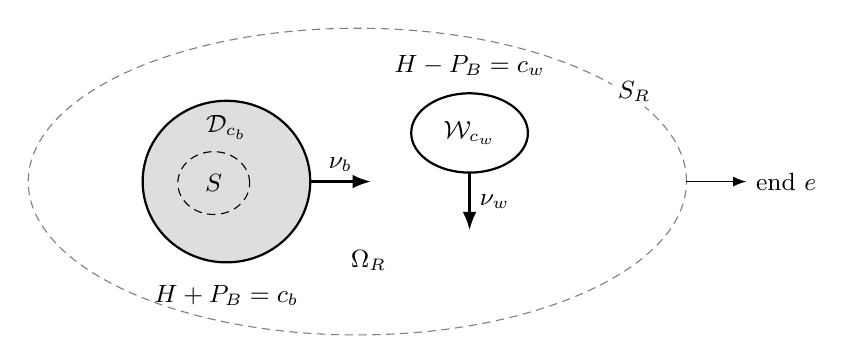
\begin{tikzpicture}[>=Latex,scale=.95,every node/.style={font=\small}]
  \draw[densely dashed,gray] (0,0) ellipse (4.4 and 2.05);
  \node[fill=white,inner sep=2pt] at (3.7,1.2) {$S_R$};
  \filldraw[fill=black!13,draw=black,thick] (-1.75,0) ellipse (1.12 and 1.08);
  \draw[densely dashed] (-1.92,-.02) ellipse (.48 and .42);
  \node at (-1.92,-.02) {$S$};
  \node at (-1.75,.72) {$\cD_{c_b}$};
  \filldraw[fill=white,draw=black,thick] (1.5,.65) ellipse (.78 and .53);
  \node at (1.5,.65) {$\cW_{c_w}$};
  \draw[->,thick] (-.63,0) -- (.18,0) node[midway,above] {$\nu_b$};
  \draw[->,thick] (1.5,.12) -- (1.5,-.65)
        node[midway,right] {$\nu_w$};
  \node at (.15,-1.05) {$\Omega_R$};
  \node at (-1.75,-1.52) {$H+P_B=c_b$};
  \node at (1.5,1.55) {$H-P_B=c_w$};
  \draw[->] (4.4,0) -- (5.2,0);
  \node[right] at (5.2,0) {end \(e\)};
\end{tikzpicture}
\caption{A schematic of the auxiliary exterior; one frontier component of
each kind is shown. The black region encloses the original boundary.
Both normals point into the retained exterior, but its black and white
faces have prescribed expansion for \(K\) and \(-K\), respectively.
The drawing represents incidence and orientations, not the topology
or dimension of the hypersurfaces.}
\label{four:fig:two-frontiers}
\end{figure}


Apply
Lemma~\ref{four:geo:stable-collar} to their respective total regions and shorten
the collars so they lie on the $\Omega$ side and are mutually disjoint.
This gives all the asserted leaf inequalities.  The support enclosure
Lemma~\ref{four:lem:support-enclosure} is available for the full families
$\cD_c$ and $\cW_c$ on $X$ and $Y$, respectively; in the latter case the
reversed black barriers remain fixed.

All these collars lie in the fixed original core $X_0$, so the lower
bound $\sigma_*$ was fixed before either threshold or any collar width.
For each collar choose a smooth profile $q_B(s)\in[0,1]$, supported in
that collar, with $q_B(s)=1-\alpha_Bs$ near its face and
$\alpha_B>0$.  Such a profile is obtained by multiplying this linear
function by a nonnegative cutoff supported before the linear function
can become negative.  With disjoint supports, define
\[
 C=a_0\sum_B\varepsilon_Bq_B(s),\qquad
 \varepsilon_B=\begin{cases}1,&B\text{ black},\\-1,&B\text{ white}.
 \end{cases}
\]
There is a finite constant $M_*$, now depending on the chosen collars and
profiles, such that $|C|\le a_0$ and $|\dd C|\le a_0M_*$.  Formula
\eqref{four:geo:linear-offsets} holds with $\kappa_B=a_0\alpha_B>0$.
Only at this point choose $a_0>0$ small enough that
\begin{equation}\label{four:geo:amplitude-budget}
 a_0(2T_*+M_*)\le\sigma_*/8.
\end{equation}
For $b_-\le h\le b_+$ we have $|h+C|\le\gamma+2a_0$, and hence on
$X_0\cap\Omega$
\begin{equation}\label{four:geo:compact-slack}
 |(h+C)\tau|+|\dd C|
 \le\gamma T_*+a_0(2T_*+M_*)\le\sigma_*/4.
\end{equation}
At points outside $\supp K$ the trace term vanishes, so this estimate
requires no restriction there on the value of $h$.

Finally choose a constant $\rho_*>0$ so small that
\[
 \rho_*\le c_0/4,\qquad
 \rho_*\max_{X_0}r^{-4-\delta_1}\le\sigma_*/4,
 \qquad \rho=\rho_* r^{-4-\delta_1}.
\]
On $X_0\cap\Omega$, \eqref{four:geo:compact-slack} plus this choice bounds the
left side of \eqref{four:eq:trace-slack} by $\sigma_*/2$.  Outside $X_0$,
$K=C=0$, and \eqref{four:geo:prepared-gap} gives the required inequality
directly.  This proves \eqref{four:eq:trace-slack}.  This order of choices uses
no lower bound on collar widths as $c_b,c_w$ approach zero: the thresholds
are chosen first, the collars next, and their amplitude last.  Ordinary
collar cutoffs also give the stated compactly supported smooth extension
of the constants $b_-$ and $b_+$.

If $D_e$ is an admissible closed connected outer domain for a cut in
$\Omega$, it is also closed in $M$, because $\Omega$ is closed in $M$.
It is a smooth codimension-zero submanifold of $M$, its interior lies in
$\operatorname{int}M$, and it contains the distant original end.  Its
entire intrinsic boundary, including every part coincident with $B$, is
therefore an admissible original enclosing cut.  Its area is at least
$A_*$.  This proves the final assertion without assuming the existence of
a minimizing cut.
\end{proof}

\section{The scalar system and exclusion of the first floor}
\label{four:sec:system}

Fix the prepared exterior and the geometric choices of
Proposition~\ref{four:prop:geometric-preparation}.  All contractions and
derivatives in this section use its background metric $g$, unless another
metric is indicated.  In particular, $\tau=\tr_gK$ is unrestricted.
The boundary normal $\nu$ points into $\Omega$.  Let $\Omega_R$ denote
the truncation at a large coordinate sphere $S_R$, so its ordinary outward
normal at its inner boundary $B$ is $-\nu$.

The purpose of the system is to produce a metric
$\ghat=e^{2t}(g+l(t)^2\dd f^2)$ with nonnegative scalar curvature and
negative boundary mean curvature.  The parameter $\eta_n$ below makes
the prescribed trace depend strictly increasingly on $f$.  A separate penalty prevents
$t$ from reaching $-\eps$.  This section proves that prevention using a
coarse height bound.  The narrower height interval needed to use
\eqref{four:eq:trace-slack} will be proved subsequently.

\subsection{Variables and a scalar-curvature identity}

Fix $0<\eps<1$ and a smooth nonincreasing function
$\vartheta:\R\to[0,1]$ equal to one on $(-\infty,0]$ and to zero on
$[1,\infty)$.  For every integer $n\ge4$ define
\begin{equation}\label{four:sys:parameters}
\begin{gathered}
 p(t)=n\vartheta(nt),\qquad
 l(t)=\exp\left(\int_0^t p(s)\,\dd s\right),\\
 L_0(t)=e^{2t}l(t),\qquad
 \ell=e^{-\eps n},\qquad \eta_n=\ell^{3/2}.
\end{gathered}
\end{equation}
Thus $0\le p\le n$, $l(t)=e^{nt}$ for $t\le0$, and $l$ is constant
with value between one and $e$ for $t\ge1/n$.  In particular
$l(-\eps)=\ell$.  The unknowns are real functions $f,Z$.  Define $t$
implicitly, and then all the remaining variables, by
\begin{equation}\label{four:sys:variables}
\begin{gathered}
 \sigma=|\grad f|,\qquad
 D=1+l(t)^2\sigma^2,\qquad d=D^{-1},\qquad
 Z=t+\frac16\log D,\qquad h=\eta_n f,\\
 w=\frac{l\grad f}{\sqrt D},\qquad a=|w|,\qquad
 v=a^2=1-d,\qquad \chi=\frac{3d}{3+pv},\\
 \Ad=\Id-w\otimes w,\qquad
 \Achi=\Id-\frac{3+p}{3+pv}w\otimes w,\qquad
 u=L_0\sqrt D.
\end{gathered}
\end{equation}
We identify vectors and covectors using $g$.  A symmetric endomorphism
also denotes the corresponding contravariant tensor, and
$|\xi|_A^2=A(\xi,\xi)$ for a covector $\xi$.
For fixed $\dd f$, the derivative of the defining expression for $Z$
with respect to $t$ is $1+pv/3\ge1$.  That expression tends to
$-\infty$ and $+\infty$ at the two ends of the real line.  It therefore
defines a unique smooth $t=t(x',Z,\dd f)$, with $x'$ the base point, for all inputs, including inputs
below the proposed floor.  No gradient bound is needed for this definition.
The eigenvalues of $\Ad$ and $\Achi$ on the line spanned by $\grad f$
are $d$ and $\chi$; their other three eigenvalues are one.  Consequently
\begin{equation}\label{four:sys:eigenvalues}
 0<\frac{3d}{3+n}\le\chi\le d\le1.
\end{equation}

Set
\begin{equation}\label{four:sys:metric-and-trace}
\begin{gathered}
 \gbar=g+l^2\dd f^2,\qquad \ghat=e^{2t}\gbar,\qquad
 H^f=\frac{l}{\sqrt D}\Hess_g f,\qquad S_f=K+H^f,\\
 F=\tr_{\Achi}S_f,\qquad
 V=u\Achi\bigl(3\grad Z+K(w,\cdot)\bigr).
\end{gathered}
\end{equation}
Where $\sigma>0$, let $e=\grad f/\sigma$.  Decompose $S_f$ into its
transverse block $T=S_f|_{e^\perp}$, mixed block
$M=S_f(e,\cdot)|_{e^\perp}$, and axial entry $j=S_f(e,e)$; write
$T^0=T-\frac13(\tr T)g|_{e^\perp}$.  Thus $\tr T=F-\chi j$.
Also write $x=e(t)$ and $y=(\dd t)|_{e^\perp}$.  The symbol $M$ in this
block notation is a covector, not the original manifold.

\begin{proposition}[Scalar identity]\label{four:sys:scalar-proposition}
For arbitrary smooth $f,Z$ and arbitrary symmetric $K$,
\begin{equation}\label{four:eq:scalar-identity}
 \frac12 e^{2t}\Scal_{\ghat}
 =\mu+J(w)+\cT+w(F)-F\tau-u^{-1}\divg_g V,
\end{equation}
where the smooth scalar $\cT$ is given, on $\{\dd f\ne0\}$, by
\begin{equation}\label{four:eq:quadratic-form}
\begin{aligned}
 \cT={}&\frac12|T^0|^2+|M+(p+1)ay|^2
       -v|y|^2+3(p+1)(|y|^2+d x^2)\\
 &-\frac13(F-\chi j)^2+\chi j^2-\chi Fj+F^2
       +2(p+1)\chi jax.
\end{aligned}
\end{equation}
The expression extends smoothly across $\{\dd f=0\}$, where any unit
axis may be used in the block expression.
\end{proposition}

\begin{proof}
We derive the identity in a stationary Lorentzian metric, keeping its
normal second form distinct from the prescribed tensor $K$.  On the
product with coordinate $s'$ use
\[
 \mathbf g=-l^2(\dd s'-\dd f)^2+\gbar.
\]
Its constant-$s'$ slices have metric $g$.  Their lapse, shift, and normal
second form, with the convention that the second form is half the normal
metric rate, are
\begin{equation}\label{four:sys:stationary-data}
 \begin{gathered}
 U=l\sqrt D,\qquad \beta=l^2\grad f=Uw,\\
 k=-\frac{\operatorname{sym}\nabla\beta}{U}
   =-H^f-p(\dd t\otimes w+w\otimes\dd t).
 \end{gathered}
\end{equation}
Here $\operatorname{sym}$ includes the factor $1/2$.  Put
$\theta=\tr_gk$, and let $N_0$ be the future unit normal.  The contracted
Gauss and normal expansion identities are
\[
 \Scal_g=\mathbf R+2\mathbf{Ric}(N_0,N_0)
                 +|k|^2-\theta^2,\qquad
 \mathbf{Ric}(N_0,N_0)=-N_0\theta-|k|^2+U^{-1}\Delta_gU.
\]
Stationarity gives $UN_0\theta=-\beta(\theta)$ and
$\divg\beta=-U\theta$.  If
\[
 \mathsf B(A,B)=A:B-(\tr_gA)(\tr_gB),\qquad
 P_A=A-(\tr_gA)g,
\]
the preceding two formulas consequently yield
\begin{equation}\label{four:sys:stationary-scalar}
 U\mathbf R=U\bigl(\Scal_g+\mathsf B(k,k)\bigr)
                   -2\divg(\grad U+\theta\beta).
\end{equation}
In the static coordinate $s'-f$ one instead has
\[
 \mathbf R=\Scal_{\gbar}-2l^{-1}\Delta_{\gbar}l,\qquad
 \Delta_{\gbar}\phi=\frac lU\divg\left(\frac Ul\Ad\grad\phi\right).
\]
Direct differentiation of $U=l\sqrt D$ gives
\[
 \grad U-\frac Ul\Ad\grad l=-k(\beta,\cdot).
\]
Moreover, using $J=\divg P_K$, symmetry of $P_K$, and
$\operatorname{sym}\nabla\beta=-Uk$ gives
\[
 \divg(P_K\beta)=U\{J(w)-\mathsf B(K,k)\}.
\]
Substitute these identities into \eqref{four:sys:stationary-scalar}, use
$\mu=(\Scal_g-\mathsf B(K,K))/2$, and put $Q=K-k$.  The result is
\begin{equation}\label{four:sys:bar-scalar}
 \frac12\Scal_{\gbar}
  =\mu+J(w)+\frac12\mathsf B(Q,Q)
       -U^{-1}\divg(UP_Qw).
\end{equation}
For example, the divergence arising directly from
\eqref{four:sys:stationary-scalar} is $U^{-1}\divg(UP_kw)$;
adding $J(w)$ combines it with $-U^{-1}\divg(UP_Kw)$ to give the
last term in \eqref{four:sys:bar-scalar}.  This also fixes its sign.

The four-dimensional conformal formula is
\[
 \frac12e^{2t}\Scal_{\ghat}
  =\frac12\Scal_{\gbar}-3\Delta_{\gbar}t-3|\dd t|_{\Ad}^2.
\]
Since
$\Delta_{\gbar}t=U^{-1}\divg(U\Ad\grad t)-p|\dd t|_{\Ad}^2$
and $u=e^{2t}U$, changing the divergence weight from $U$ to $u$ gives
\begin{equation}\label{four:sys:pretrace-identity}
\begin{aligned}
 \frac12e^{2t}\Scal_{\ghat}
 ={}&\mu+J(w)+\frac12\mathsf B(Q,Q)+2P_Q(w,\grad t)
               +3(p+1)|\dd t|_{\Ad}^2\\
 &-u^{-1}\divg\bigl(u(P_Qw+3\Ad\grad t)\bigr).
\end{aligned}
\end{equation}
The following differential identities follow from \eqref{four:sys:variables}:
\begin{equation}\label{four:sys:differential-identities}
\begin{aligned}
 3\dd Z&=(3+pv)\dd t+H^f(w,\cdot),\\
 \divg w&=\tr_{\Ad}H^f+p d\,w(t),\\
 \dd\log u&=(p+2+pv)\dd t+H^f(w,\cdot).
\end{aligned}
\end{equation}
They imply
\begin{equation}\label{four:sys:trace-divergence}
\begin{aligned}
 \frac Vu&=P_Qw+3\Ad\grad t+Fw,\\
 u^{-1}\divg(uw)
  &=\tr_gH^f+2(p+1)w(t)\\
  &=F+(1-\chi)j-\tau+2(p+1)w(t).
\end{aligned}
\end{equation}
Adding $uFw$ inside the divergence in
\eqref{four:sys:pretrace-identity} therefore leaves
$w(F)+F u^{-1}\divg(uw)$.  Its trace contribution is exactly
$-F\tau$, while the remaining quadratic expression is
\begin{equation}\label{four:sys:invariant-quadratic}
\begin{aligned}
 \cT={}&\frac12\mathsf B(Q,Q)+2P_Q(w,\grad t)
          +3(p+1)|\dd t|_{\Ad}^2\\
 &+F\left(F+\frac{3+p}{3+pv}S_f(w,w)+2(p+1)w(t)\right).
\end{aligned}
\end{equation}
This is smooth even at $w=0$, since
$(1-\chi)j=(3+p)S_f(w,w)/(3+pv)$.  For the block expansion, $Q$ has
blocks $T$, $M+pay$, $j+2pax$, and $\tr T=F-\chi j$.
Expanding \eqref{four:sys:invariant-quadratic} gives
\eqref{four:eq:quadratic-form}.  At $w=0$ it reduces to
\[
 \cT=\frac12\bigl(|S_f|^2+(\tr_gS_f)^2\bigr)
                      +3(p+1)|\dd t|^2,
\]
which is independent of the auxiliary axis.  This proves all assertions.
\end{proof}

\subsection{Coercivity and the boundary identity}

Throughout the proof, $\Pi_n$ denotes a bound of the form
$C(1+n)^N$ for a finite nonnegative integer $N$.  Its coefficient $C$ and
exponent $N$ may depend on the fixed prepared data, $\eps$, the chosen
collars and smooth switches, and any explicitly fixed small absorption
constant.  They never depend on $R$, a homotopy parameter, or a solution.
Different occurrences may denote larger such bounds.  Constants denoted
by $C(n)$ in later fixed-$n$ analytic estimates have no polynomial
restriction and will not enter a limit requiring polynomial control.

\begin{lemma}[Polynomial coercivity]\label{four:sys:coercivity-lemma}
For all inputs in \eqref{four:sys:variables},
\begin{equation}\label{four:eq:coercivity}
 |T|^2+|M|^2+d j^2+F^2+|\dd t|_{\Ad}^2\le\Pi_n\cT.
\end{equation}
At a point where $\dd t=0$, there are absolute constants $c,C>0$ such
that
\begin{equation}\label{four:sys:stationary-coercivity}
 \begin{aligned}
 c\bigl(|T^0|^2+|M|^2+\chi j^2+F^2\bigr)&\le\cT\\
 &\le C\bigl(|T^0|^2+|M|^2+\chi j^2+F^2\bigr).
 \end{aligned}
\end{equation}
\end{lemma}

\begin{proof}
Completing squares in \eqref{four:eq:quadratic-form} gives the exact identity
\begin{equation}\label{four:sys:exact-squares}
\begin{aligned}
 \cT={}&\frac12|T^0|^2+|M+(p+1)ay|^2
        +\bigl(3(p+1)-v\bigr)|y|^2\\
 &+3(p+1)d\left(x+\frac{\chi a j}{3d}\right)^2
       +\frac23\left(F-\frac{\chi j}{4}\right)^2
       +\frac{d(48-3d)}{8(3+pv)^2}j^2.
\end{aligned}
\end{equation}
For the final coefficient, the identity used in this completion is
\[
 \chi-\frac38\chi^2-\frac{(p+1)\chi^2v}{3d}
                 =\frac{d(48-3d)}{8(3+pv)^2}.
\]
The coefficient of $|y|^2$ is at least two, and the last coefficient is
at least $45d/[8(3+n)^2]$.  Thus $d j^2\le C(3+n)^2\cT$.
The inequalities $\chi^2\le d^2\le d$ then recover $F^2$ from its
shifted square and $d x^2$ from its shifted square, at polynomial cost.
Recovering $M$ costs at most $C(1+n)^2|y|^2$, and recovering $T$ uses
$\tr T=F-\chi j$.  This proves \eqref{four:eq:coercivity}; these observations,
for instance, allow one common bound $C(1+n)^2$ in that inequality.

When $\dd t=0$, complete only the $(F,j)$ terms to obtain
\begin{equation}\label{four:sys:stationary-squares}
 \cT=\frac12|T^0|^2+|M|^2
      +\frac23\left(F-\frac{\chi j}{4}\right)^2
      +\chi\left(1-\frac{3\chi}{8}\right)j^2.
\end{equation}
Since $5/8\le1-3\chi/8\le1$ and $\chi^2\le\chi$, this gives
\eqref{four:sys:stationary-coercivity} with absolute constants.
\end{proof}

\begin{lemma}[Boundary conversion]\label{four:sys:boundary-lemma}
On any smooth face on which $f$ is constant, let
$P_B=\tr_BK$, $w_\nu=\inner{w}{\nu}$, and let $H$ be its background
mean curvature for the normal into $\Omega$.  Then
\begin{equation}\label{four:eq:boundary-identity}
 \frac{V_\nu}{u}
   =d(H+3\partial_\nu t)-H+w_\nu(F-P_B),\qquad
 \widehat H=e^{-t}\sqrt d\,(H+3\partial_\nu t).
\end{equation}
\end{lemma}

\begin{proof}
With $\mathrm{II}_B(X,Y)=g(\nabla_X\nu,Y)$ for tangent vectors,
one has tangentially $\Hess f=(\partial_\nu f)\mathrm{II}_B$, so
$\tr T=P_B+w_\nu H$ and
$\chi j=F-P_B-w_\nu H$.  Use this relation in the first identity of
\eqref{four:sys:trace-divergence}; as $w$ is normal on the face, it gives
\[
 V_\nu/u=3d\partial_\nu t+w_\nu(F-P_B-w_\nu H),
\]
which is the first assertion because $w_\nu^2=1-d$.  The induced
metric of $\gbar$ on the face equals $g|_B$, and its normal in base
coordinates is $\sqrt d\,\nu$.  In the tangential first variation,
$l^2\dd f^2$ contributes zero since the tangential derivatives of $f$
vanish there.  Hence $H_{\gbar}=\sqrt d\,H$.  Applying the boundary
conformal formula with $\nu_{\gbar}=\sqrt d\,\nu$ proves the second
assertion.  Both assertions also hold when $\dd f=0$.
\end{proof}

\subsection{The equations and their four-stage homotopy}

Extend the end radius to a positive smooth function $r\ge1$ on $\Omega$
and set
\begin{equation}\label{four:sys:source}
\begin{gathered}
 \rho_0=r^{-4-\delta_1},\qquad \rho_1=r^{-3},\qquad
 m_0(t)=\vartheta\bigl(n(t+\eps)\bigr),\qquad
 \cP=C_n(\rho_0+v\rho_1),\\
 \Xi=\delta_0\cT+\rho+\delta_0\eta_n a\sigma-m_0(t)\cP.
\end{gathered}
\end{equation}
The constant $\delta_0>0$ and the polynomial $C_n$ will be fixed in
Proposition~\ref{four:prop:floor-exclusion}.  The smooth positive weight
$\rho$ comes from \eqref{four:eq:trace-slack}; in particular
$\rho\le C\rho_0$.  The combination
$a\sigma=l|\dd f|^2/\sqrt D$ is smooth also at $\dd f=0$, so all
terms of $\Xi$ are smooth functions of the indicated jets.
Choose a constant $N_B>1+\sup_B|H|$, and put
\[
 \cB=-H+w_\nu(F-P_B)-N_Bd.
\]
The desired system is
\begin{equation}\label{four:eq:system}
\begin{cases}
 F=h+C, &\text{in }\Omega_R,\\
 \divg V=u\Xi, &\text{in }\Omega_R,\\
 h=b,\quad V_\nu/u=\cB, &\text{on }B,\\
 f=Z=0, &\text{on }S_R.
\end{cases}
\end{equation}
In every boundary flux expression the symbol $F$ is evaluated using the
prescribed trace right side.  Thus the boundary condition contains no
second derivative of $f$.  For a solution of \eqref{four:eq:system},
\eqref{four:eq:boundary-identity} immediately gives
$\widehat H=-e^{-t}\sqrt d\,N_B<0$.

We specify the entire homotopy because its boundary modifications and
strictly increasing height term will be used in the a priori estimates.
The stages run from the desired system to the terminal problem with
solution $f=Z=0$; Section~\ref{four:sec:existence} transfers existence back
along this homotopy.  Take a smooth
$j_0:\R\to[0,1]$ which is zero for $t\le0$ and one for $t\ge1$.
For $0\le\lambda\le1$ put
\[
 V_\lambda=u\Achi\bigl(3\grad Z+\lambda K(w,\cdot)\bigr).
\]
In stages 1--3 use
\begin{equation}\label{four:eq:homotopy-flux}
\begin{cases}
 \divg V_\lambda=u\Xi &\text{in }\Omega_R,\\
 (V_\lambda)_\nu/u=
 [1-(1-\lambda)j_0(t)]
 [\cB-(1-\lambda)(\Achi K(w,\cdot))_\nu]
 &\text{on }B.
\end{cases}
\end{equation}
Keep the outer data $f=Z=0$ throughout.

Here are explicit smooth choices of the auxiliary trace terms.  Fix
$0<4\xi_1<b_+-b_-$ and smooth height switches $q_-,q_+$ such that
\[
\begin{array}{lll}
 q_-(z)=1 &(z\le b_-+\xi_1),&q_-(z)=0\quad(z\ge b_-+2\xi_1),\\
 q_+(z)=0 &(z\le b_+-2\xi_1),&q_+(z)=1\quad(z\ge b_+-\xi_1),
\end{array}
\]
where $q_-$ is nonincreasing and $q_+$ is nondecreasing.  Choose a smooth
direction switch $q_d$ with values in $[0,1]$, equal to one on
$(-\infty,-3/4]$ and zero on $[-1/2,\infty)$.  On each collar write
$N=\grad s/|\dd s|$, so $N=\nu$ at the face, and choose a smooth cutoff $\omega_B$ supported
there and equal to one near the face.  The collars are disjoint.  With
fixed constants
\[
 A_0>2\sup_B|H|+1,\qquad A_1>\sup_B|H|+1,
\]
define, extending by zero outside the collars,
\begin{equation}\label{four:sys:switches}
\begin{aligned}
 D_0(x',w,z)
  &=-A_0\omega_B(x')q_d(w\cdot N)q_-(z)
                      &&\text{on black collars},\\
 D_0(x',w,z)
  &= A_0\omega_B(x')q_d(-w\cdot N)q_+(z)
                      &&\text{on white collars},\\
 D_1(x',w)&=A_1\omega_B(x')\,w\cdot N
                      &&\text{on every collar}.
\end{aligned}
\end{equation}
Both terms vanish at $w=0$, are bounded for $|w|\le1$, and have bounded
derivatives of every order on bounded height ranges.  These bounds are
independent of $n$.  In addition $\partial_zD_0\ge0$.

The successive trace prescriptions and inner Dirichlet data are as
follows; the indicated parameter moves in the displayed direction.
\begin{enumerate}[label=\textup{Stage \arabic*:},leftmargin=*]
\item Decrease $\lambda$ from one to zero, keeping
      $F=h+C$ and $h|_B=b$.
\item Keep $\lambda=0$, increase $\alpha_0$ from zero to one, and use
      $F=h+C+\alpha_0D_0(x',w,h)$ and $h|_B=b$.
\item Keep $\lambda=0$, increase $\zeta$ from zero to one, and use
\begin{equation}\label{four:sys:trace-prescriptions}
\begin{aligned}
 F={}&h+(1-\zeta)\bigl[C+D_0(x',w,h+\zeta b(x'))\bigr]\\
    &+\zeta\bigl[\tr_{\Achi}K+D_1(x',w)\bigr],
 \qquad h|_B=(1-\zeta)b.
\end{aligned}
\end{equation}
\item Retain the terminal prescription
      $F=h+\tr_{\Achi}K+D_1$ and $h|_B=0$.  Keep $\lambda=0$ and
      multiply both right sides of \eqref{four:eq:homotopy-flux} by a common
      parameter $\gamma$, decreasing from one to zero.
\end{enumerate}
The endpoints agree, so this is a continuous homotopy.  All trace right
sides have derivative at least one with respect to $h$, with $(x',w,t)$
fixed.  This is also the relevant derivative when comparing scalar
solutions at a shared gradient and shared $Z$, since $t$ is independent
of the value of $f$.

Two consequences of these choices will be useful.  First, at a stage 3
face, evaluate the prescribed right side at $h=(1-\zeta)b$ and at the
limiting values $w=\pm\nu$, $d=\chi=0$.  It obeys
\begin{equation}\label{four:sys:direction-inequalities}
 F(\nu)\ge P_B+H,\qquad F(-\nu)\le P_B-H.
\end{equation}
Indeed, on a black face $b+C=P_B+H$, $D_0(\nu,b)=0$, and
$D_0(-\nu,b)=-A_0$; on a white face $b+C=P_B-H$,
$D_0(-\nu,b)=0$, and $D_0(\nu,b)=A_0$.  The terminal expressions are
$P_B\pm A_1$.  Each inequality follows for both endpoints from the
choices of $A_0,A_1$, and hence for their convex combination.

Second, throughout stage 4 the scalar solution is $f=0$, for every trial
$Z$.  Its equation is
$\tr_{\Achi}H^f=\eta_n f+D_1$, with zero boundary values.  At a
positive interior maximum $w=0$, $D_1=0$, $\Achi=\Id$, and
$l\Delta f=\eta_n f>0$, a contradiction; a negative minimum is
excluded in the same way.  Consequently in this stage
\begin{equation}\label{four:sys:terminal-system}
 f=0,\quad t=Z,\quad
 \cT=\cT_K+3(p+1)|\dd t|^2,\qquad
 \cT_K=\tfrac12(|K|^2+\tau^2),
\end{equation}
and its two remaining equations are exactly
\[
 \divg(3u\grad t)=\gamma u\Xi,\qquad
 3\partial_\nu t=\gamma[1-j_0(t)](-H-N_B).
\]

\subsection{Coarse heights and an outer boundary estimate}

\begin{lemma}[Height bound before the floor]\label{four:lem:coarse-height}
There exist fixed $r_0$ and $C_*>0$, independent of $n$, $R$, and all
homotopy parameters, with the following property.  Every smooth solution
of the trace equation in any stage, with its prescribed Dirichlet data,
on $\Omega_R$ for $R\ge2r_0$ satisfies
\begin{equation}\label{four:sys:coarse-height}
 |h|+|F|\le C_*,\qquad
 |h|\le C_*(r^{-3/2}-R^{-3/2})\quad(r_0\le r\le R).
\end{equation}
Here $Z$ may be arbitrary; the divergence equation and the condition
$t\ge-\eps$ are not assumed.  In particular, with the prescribed outer
value $Z=0$,
\begin{equation}\label{four:sys:outer-gradient}
 |\grad f|\le C_*\eta_n^{-1}R^{-5/2}\quad\text{on }S_R.
\end{equation}
For every fixed $n$ there is $R_{\min}(n)\ge2r_0$, chosen to tend to
infinity with $n$, such that every such solution for $R\ge R_{\min}(n)$
has
\begin{equation}\label{four:sys:outer-floor}
 t> -\eps\quad\text{on }S_R.
\end{equation}
\end{lemma}

\begin{proof}
At an interior extremum of $h$, $w=0$ and both auxiliary terms vanish.
The trace equation becomes
\[
 l\Delta f=h+C-\tau\quad\text{in stages 1 and 2},\qquad
 l\Delta f=h+(1-\zeta)(C-\tau)\quad\text{in stage 3}.
\]
Since $l>0$, comparison at a maximum and a minimum bounds $|h|$ by
$\max(\sup_B|b|,\|C-\tau\|_\infty)$.  Stage 4 has $h=0$.
All prescribed trace right sides then bound $|F|$ by a fixed constant,
because $D_0,D_1$ are bounded and $\|\Achi\|\le1$.

Choose $r_0$ beyond the supports of $K,C,b,D_0,D_1$.  At a comparison
with a radial function, the axis of $\Achi$ is
$\grad_g r/|\dd r|_g$.  Uniformly for $0<\chi\le1$, the prepared end
expansion gives
\begin{equation}\label{four:sys:radial-trace}
 \tr_{\Achi}\Hess_g r^{-3/2}
 =\frac32\left(-3+\frac52\chi\right)r^{-7/2}
                +O(r^{-11/2})<0
\end{equation}
after increasing $r_0$.  The leading coefficient is at most $-3/4$,
so the choice is independent of $n$.  Take $C_*$ large enough that
$C_*(r_0^{-3/2}-R^{-3/2})$ dominates the global height bound for every
$R\ge2r_0$.  On this annulus the scalar equation is
\[
 \frac{l}{\eta_n\sqrt D}\tr_{\Achi}\Hess_g h=h.
\]
The functions $\pm C_*(r^{-3/2}-R^{-3/2})$ are respectively upper and
lower barriers by \eqref{four:sys:radial-trace}.  At a putative first
comparison point the gradients coincide, so the same positive trace
matrix and the same positive prefactor occur in both expressions.
The Hessian order and the proper height sign give a contradiction.
This proves the end estimate.  Differentiating the comparison at the
outer boundary, where $h=0$ tangentially, gives
\eqref{four:sys:outer-gradient}, absorbing the uniform end normal comparison
into $C_*$.

Finally let $G(t)=t+\frac16\log(1+l(t)^2\sigma^2)$ at an outer point.
It is strictly increasing and $G(t)=Z=0$.  Thus $t>-\eps$ if
\[
 G(-\eps)=-\eps+\frac16\log(1+\ell^2\sigma^2)<0.
\]
By \eqref{four:sys:outer-gradient}, it suffices to choose
$R_{\min}(n)$ so large that
$C_*^2\ell^2\eta_n^{-2}R_{\min}(n)^{-5}<e^{6\eps}-1$.
This uses only fixed-$n$ enlargement of the outer radius.
\end{proof}

\subsection{The stationary comparison at a minimum of \texorpdfstring{$t$}{t}}

The scalar identity is useful at a floor contact because a second,
Riemannian Gauss calculation gives an upper bound for the same scalar
curvature.  Define, for a symmetric tensor $A$ and a chosen unit axis $e$,
\begin{equation}\label{four:sys:gauss-quadratic}
 \mathcal S(A)=\frac13(\tr_\perp A)^2
       -\frac12|A_\perp^0|^2
       +d A_{ee}\tr_\perp A-d|A_{e\perp}|^2.
\end{equation}

\begin{lemma}[Stationary Gauss comparison]\label{four:sys:gauss-lemma}
At an interior local minimum of $t$,
\begin{equation}\label{four:sys:gauss-bound}
 \frac12e^{2t}\Scal_{\ghat}
 \le\frac12\Scal_g-v\Ric_g(e,e)+\mathcal S(H^f).
\end{equation}
At every point where $\dd t=0$ there are an absolute $c_2>0$ and a
polynomial bound $\Pi_n$ such that
\begin{equation}\label{four:sys:floor-coercivity}
 \cT-\mathcal S(H^f)
          \ge c_2\cT-\Pi_n\bigl(vF^2+|K|^2\bigr).
\end{equation}
These conclusions extend to $\dd f=0$ with any unit axis.
\end{lemma}

\begin{proof}
Use the Riemannian warped product $g+l^2(\dd b')^2$ and its graph
$b'=f$.  At $\dd t=0$ one has $\dd l=0$, so the graph second form is
$H^f$, up to its immaterial overall sign.  Its inverse metric is $\Ad$.
The contracted second-form contribution is
\[
 \tfrac12\{(\tr_{\Ad}H^f)^2-|H^f|_{\Ad\otimes\Ad}^2\}
   =\mathcal S(H^f),
\]
as is seen by writing $\Ad=\operatorname{diag}(1,1,1,d)$.
The ambient scalar curvature and Ricci blocks are
\[
 \Scal_g-2\Delta l/l,\qquad
 \Ric_g-\Hess l/l,\qquad -\Delta l/l,
\]
for the scalar, horizontal block, and unit vertical direction;
the mixed block is zero.  The graph unit normal has horizontal part
$-w$ and vertical component $\sqrt d$.  Therefore the ambient scalar
minus twice its normal Ricci, divided by two, is
\[
 \frac12\Scal_g-v\Ric_g(e,e)
                     -v\tr_\perp(\Hess l/l).
\]
At a stationary point $\Hess l/l=p\Hess t$, and the conformal term
is $-3\tr_{\Ad}\Hess t$.  Thus we have, more precisely, the equality
\begin{equation}\label{four:sys:stationary-gauss-exact}
\begin{aligned}
 \frac12e^{2t}\Scal_{\ghat}
 ={}&\frac12\Scal_g-v\Ric_g(e,e)+\mathcal S(H^f)\\
 &-(3+pv)\tr_\perp\Hess_g t-3d\Hess_g t(e,e).
\end{aligned}
\end{equation}
At a minimum the last two terms are nonpositive, proving
\eqref{four:sys:gauss-bound}.

For \eqref{four:sys:floor-coercivity}, first subtract $\mathcal S(S_f)$.
An expansion using $\tr T=F-\chi j$ gives exactly
\begin{equation}\label{four:sys:stationary-difference}
\begin{aligned}
 \cT-\mathcal S(S_f)
 ={}&|T^0|^2+(1+d)|M|^2
       +\chi(1+d-2\chi/3)j^2\\
 &+(\chi/3-d)Fj+F^2/3.
\end{aligned}
\end{equation}
At $d=\chi=1$ the $(F,j)$ quadratic is
$F^2/3-2Fj/3+4j^2/3$, whose matrix has determinant $1/3$ and positive
trace.  It is uniformly positive in a fixed neighborhood of this point.
Since
\[
 1-d=v,\qquad 1-\chi=\frac{(3+p)v}{3+pv},
\]
there is an absolute $\kappa_0>0$ such that this neighborhood contains
all inputs with $(1+p)v\le\kappa_0$.  In that region
\eqref{four:sys:stationary-difference} controls an absolute fraction of
$|T^0|^2+|M|^2+\chi j^2+F^2$.

In the remaining region, use
$\chi(1+d-2\chi/3)\ge\chi$ and $|\chi/3-d|\le d$ to absorb the
mixed term into, for example, $\chi j^2/4$ and a multiple of
$(d^2/\chi)F^2$.  The only ratio required is
\begin{equation}\label{four:sys:polynomial-ratios}
 \frac{d^2}{\chi}=\frac{d(3+pv)}3\le\frac{3+n}{3},\qquad
 v>\frac{\kappa_0}{1+p}\ge\frac{\kappa_0}{1+n}.
\end{equation}
Keeping also a fixed fraction of $F^2$ at the cost of another multiple
of $F^2$, this proves a lower bound by an absolute fraction of the
stationary norm minus $C(1+n)^2vF^2$.  Equation
\eqref{four:sys:stationary-coercivity} converts the norm to $\cT$.

It remains to replace $S_f$ by $S_f-K$.  Polarizing
\eqref{four:sys:gauss-quadratic} bounds the difference by
\[
 C\bigl(|T|+d|j|+d|M|\bigr)|K|+C|K|^2.
\]
The stationary norm controls $|T|$ and $|M|$, while
$d|j|\le(d^2/\chi)^{1/2}(\chi j^2)^{1/2}$.
By \eqref{four:sys:polynomial-ratios} and Young's inequality, for every
fixed $\alpha>0$ this is at most
$\alpha\cT+C_\alpha(1+n)|K|^2$.  Choose $\alpha$ to retain half
the already obtained positive coefficient of $\cT$.  This proves
\eqref{four:sys:floor-coercivity} with absolute $c_2>0$.
\end{proof}

\begin{lemma}[Errors from the trace switches and drift]
\label{four:sys:stationary-errors}
Let $\mathcal K$ be a fixed compact enlargement of the supports of
$K,C,b,D_0,D_1$.  For every fixed $\delta_2>0$, every smooth trace
solution in stages 1--3 satisfies, at a point where $\dd t=0$,
\begin{equation}\label{four:sys:derivative-errors}
\begin{aligned}
 w(F)&\ge\eta_n a\sigma-\delta_2\cT-\Pi_n\mathbf1_{\mathcal K},\\
 u^{-1}\bigl|\divg(u\Achi K(w,\cdot))\bigr|
   &\le\delta_2\cT+\Pi_n\mathbf1_{\mathcal K}.
\end{aligned}
\end{equation}
The polynomial may depend on $\delta_2$ and the fixed geometric choices,
but no negative power of $\ell$ or $\eta_n$ is required.
\end{lemma}

\begin{proof}
At $\dd t=0$, differentiation gives
\[
 \nabla_iw=\Ad H^f_{i\cdot},\qquad
 \dd\log u=H^f(w,\cdot),\qquad \dd p=p'(t)\dd t=0.
\]
These formulas and \eqref{four:sys:stationary-coercivity} show
\begin{equation}\label{four:sys:stationary-derivatives}
 |\nabla w|+|\dd\log u|_{\Achi}+|\nabla\Achi|
                  \le\Pi_n(\sqrt{\cT}+|K|).
\end{equation}
For clarity, the axial entry in $\nabla w$ is $dH^f_{ee}$, and its
control uses $d^2/\chi\le(3+n)/3$.  In $|\dd\log u|_{\Achi}$
the axial entry has the factor $\sqrt\chi$.  Differentiating
$\Achi=\Id-(3+p)w\otimes w/(3+pv)$ uses only the preceding
$\nabla w$ and coefficients bounded by powers of $1+n$, since
$3+pv\ge3$.  This proves \eqref{four:sys:stationary-derivatives} without
dividing by $l$ or $\eta_n$.

Write the relevant prescribed trace as $\Phi(x',w,t,h)$.  Its height
derivative is at least one, so the chain rule contains the favorable term
\[
 \Phi_h w(h)\ge w(h)=\eta_n a\sigma.
\]
All other terms are supported in $\mathcal K$.  Lemma~\ref{four:lem:coarse-height}
bounds their height arguments in a fixed range; derivatives of $D_0,D_1$
and $b$ are consequently bounded.  Derivatives of $\tr_{\Achi}K$ use
$\nabla K$ and \eqref{four:sys:stationary-derivatives}.  The $t$ derivative
has zero contribution at the point in question.  Thus the remaining
absolute error is bounded by $\Pi_n(1+\sqrt{\cT})\mathbf1_{\mathcal K}$.
Young's inequality proves the first assertion.

Expanding the divergence in the second assertion differentiates
$\Achi$, $K$, and $w$, and adds
$\inner{K(w,\cdot)}{\dd\log u}_{\Achi}$.
The latter is bounded by $C|K|\,|\dd\log u|_{\Achi}$.
Equation~\eqref{four:sys:stationary-derivatives}, compact support, and Young's
inequality give the second assertion with the same allowed dependencies.
\end{proof}

\subsection{Exclusion of first contact with the floor}

\begin{proposition}[First-floor exclusion]\label{four:prop:floor-exclusion}
There are a fixed $\delta_0>0$ and a positive polynomial $C_n$ in
\eqref{four:sys:source} such that, for every $n\ge4$ and every
$R\ge R_{\min}(n)$, no smooth solution at any stage of the homotopy
satisfies
\[
 \min_{\overline\Omega_R}t=-\eps.
\]
The choices depend only on the prepared data, $\eps$, and the fixed
switches and collars.  They do not use a height bound sharper than
Lemma~\ref{four:lem:coarse-height}.
\end{proposition}

\begin{proof}
Suppose first that a floor minimum is interior and the parameter is in
one of stages 1--3.  At that point $\dd t=0$ and $\Hess t\ge0$.
Subtract \eqref{four:sys:gauss-bound} from \eqref{four:eq:scalar-identity} and
use $V_\lambda=V-(1-\lambda)u\Achi K(w,\cdot)$.  This gives
\begin{align*}
 u^{-1}\divg V_\lambda\ge{}&
 \mu-\tfrac12\Scal_g+J(w)+v\Ric_g(e,e)
        +\cT-\mathcal S(H^f)+w(F)-F\tau\\
 &-(1-\lambda)u^{-1}\divg(u\Achi K(w,\cdot)).
\end{align*}
Choose $\delta_2>0$ in Lemma~\ref{four:sys:stationary-errors} so small that
the two losses $\delta_2\cT$ leave at least $c_2\cT/2$ in
\eqref{four:sys:floor-coercivity}.  The remaining tensor expressions
$\mu-\Scal_g/2=(\tau^2-|K|^2)/2$, $J$, and $F\tau$ are compactly
supported and bounded by fixed constants, using
Lemma~\ref{four:lem:coarse-height}.  On the complement of $\mathcal K$,
$F=h$ and $F^2\le C r^{-3}$; also
$|\Ric_g|\le C r^{-4}$.  On $\mathcal K$ the positive weight
$\rho_0$ has a fixed positive minimum.  Hence
\[
 \mathbf1_{\mathcal K}+vF^2+v|\Ric_g|
                   \le C(\rho_0+v\rho_1).
\]
Combining these bounds yields an absolute $c_3>0$ and a polynomial
$Q_n\ge0$ such that, at the proposed minimum,
\begin{equation}\label{four:sys:floor-divergence-lower}
 u^{-1}\divg V_\lambda
   \ge c_3\cT+\eta_n a\sigma-Q_n(\rho_0+v\rho_1).
\end{equation}
Fix
$0<\delta_0<\min(c_3/2,1/4)$.
Since $t=-\eps$ gives $m_0(t)=1$, choose $C_n$ to exceed
$Q_n+1+\sup_\Omega(\rho/\rho_0)$.  The right side of
\eqref{four:sys:floor-divergence-lower} then strictly exceeds
$\delta_0\cT+\rho+\delta_0\eta_n a\sigma-C_n(\rho_0+v\rho_1)
=\Xi$, contradicting \eqref{four:eq:homotopy-flux}.  This choice is
polynomial in $n$.

At an interior minimum in stage 4, \eqref{four:sys:terminal-system} gives
$f=0$, $t=Z$, and $v=0$.  If $\gamma>0$, its equation at the
stationary point is
\[
 3\Delta t=\gamma\bigl(\delta_0\cT_K+\rho-C_n\rho_0\bigr).
\]
Enlarge $C_n$, still polynomially, so that
$C_n>1+\sup_\Omega(\delta_0\cT_K+\rho)/\rho_0$.
The right side is strictly negative, contradicting $\Delta t\ge0$.
This additional bound is finite because $K$ is compactly supported.

Consider next an inner boundary minimum in stages 1--3.
There $j_0(-\eps)=0$, so the same drift correction appears on both
sides of \eqref{four:eq:homotopy-flux}.  Cancelling it gives $V_\nu/u=\cB$.
Equation~\eqref{four:eq:boundary-identity} and $d>0$ imply
\[
 3\partial_\nu t=-H-N_B<0.
\]
This contradicts the nonnegative derivative into $\Omega_R$ at a
boundary minimum.  In stage 4 with $\gamma>0$, the corresponding exact
formula from \eqref{four:sys:terminal-system} is
$3\partial_\nu t=\gamma(-H-N_B)<0$, giving the same contradiction.
The outer boundary is excluded by \eqref{four:sys:outer-floor}.

Finally, at $\gamma=0$, $f=0$ and the remaining problem is
$\divg(3u\grad t)=0$ with homogeneous inner conormal data and $t=0$
on $S_R$.  Testing by $t$ gives $\int_{\Omega_R}3u|\dd t|^2=0$.
Connectedness and the nonempty Dirichlet boundary imply $t=0$.
Thus no stage admits floor equality.
\end{proof}

The order of choices is now fixed: choose the background geometric
data and $\eps$, then $\delta_0$ and the polynomial penalty $C_n$.
At each $n$, enlarge the outer radius as in
Lemma~\ref{four:lem:coarse-height}.  Subsequent estimates may increase the
lower bound on $n$ or $R_{\min}(n)$, but none will replace $C_n$ by an
arbitrary fixed-$n$ constant.  In particular, the first-floor argument
has paid for $F\tau$ using a bounded compact error and has not used the
eventual small-height absorption in \eqref{four:eq:trace-slack}.

\section{Height separation and global bounds}\label{four:sec:bounds}

Throughout this section the prepared geometry, its thresholds and collars,
and $\eps\in(0,1)$ are fixed.  We consider arbitrary smooth solutions of
the four stages of the homotopy in Section~\ref{four:sec:system}, on
$\Omega_R$, satisfying $t\ge-\eps$.  The admissible radii satisfy
$R\ge R_{\min}(n)$, where $R_{\min}(n)\to\infty$ and is large enough for
the outer-boundary conclusion of Proposition~\ref{four:prop:floor-exclusion}.
Every assertion of uniformity includes the homotopy parameter and $R$.
As in Remark~\ref{four:rem:constants}, $\Pi_n$ denotes a polynomial bound in
$n$, whereas $C(n)$ can depend arbitrarily on the fixed integer $n$.
We shall keep this distinction through the boundary-flux estimate.

\subsection{The limiting heights and the two total regions}

The large factor $l/\eta_n$ forces a nonconstant test level of $h$ to
approach a hypersurface whose expansion is controlled by the trace
equation.  A sublevel of the relaxed limiting height need not have a
regular boundary.  We first establish the expansion inequality for
every smooth exterior support, including at a plateau and at a face
of the opposite color.

\begin{proposition}[Separation from the two total regions]
\label{four:prop:height-exclusion}
Let $A\subset\overline\Omega$ be compact.  In the first two homotopy
stages the following statements hold.
\begin{enumerate}[label=\textup{(\roman*)}]
\item If $A\cap\cD_{c_b}=\varnothing$, there exist $\xi_A>0$ and
$n_A$ such that $h\ge b_-+\xi_A$ on $A$ for every $n\ge n_A$.
\item If $A\cap\cW_{c_w}=\varnothing$, there exist $\xi_A>0$ and
$n_A$ such that $h\le b_+-\xi_A$ on $A$ for every $n\ge n_A$.
\end{enumerate}
Here the total regions are the full closed regions of
Proposition~\ref{four:prop:geometric-preparation}, including components whose
frontiers do not border $\Omega$.
\end{proposition}

\begin{proof}
We give the lower-height argument first.  Consider any sequence
$n_i\to\infty$ of the indicated solutions; its radii tend to infinity.
Extend $h_i$ by the constant $b_+$ into a small collar across each white
face.  The functions on these enlarged neighborhoods are continuous.
Define their lower relaxed limit by
\[
 \underline h(x)=\liminf_{\substack{i\to\infty\\y\to x}}h_i(y).
\]
It is lower semicontinuous and locally bounded by
Lemma~\ref{four:lem:coarse-height}.  Fix levels
\begin{equation}\label{four:bnd:levels}
 b_-<k<k'<\min\{0,b_-+\xi_1\},\qquad k'+a_0<0,
\end{equation}
where $\xi_1$ is the height-cutoff constant in $D_0$.
We initially work away from black faces.

Suppose a smooth $\phi$ touches $\underline h$ from below at $x$,
with $\underline h(x)<k'$ and $\dd\phi(x)\ne0$.  Subtracting a small
fourth-order function of distance makes the contact strict on a
small closed neighborhood without changing its second jet.  The
definition of the relaxed limit and minimization on this neighborhood
give, after passing to a subsequence, points $x_i\to x$ and constants $c_i$ such that $\phi+c_i$
touches $h_i$ from below at $x_i$, and
$h_i(x_i)\to\underline h(x)$.  These contacts are interior contacts of
the original exterior: their heights are eventually strictly below
$k'<b_+$, so they cannot occur on a white face or in its constant
extension.  This remains true when $x$ itself is on a white face.

At contact, $\dd h_i=\dd\phi$ and
$\Hess h_i\ge\Hess\phi$.  The positive trace matrix therefore gives
\begin{equation}\label{four:bnd:test-trace}
 \tr_{A_{\chi_i}}K+
 \frac{1}{\sqrt{(\eta_{n_i}/l_i)^2+|\dd\phi|^2}}
       \tr_{A_{\chi_i}}\Hess\phi
 \le h_i+C+\alpha_iD_0,
 \qquad 0\le\alpha_i\le1.
\end{equation}
Here $\alpha_i=0$ in the first stage.  The cutoff construction gives
$D_0\le0$ at these low heights, everywhere: its white contribution
vanishes there, and its black contribution is nonpositive.  Moreover
\[
 \frac{l_i}{\eta_{n_i}}\ge
 \frac{\ell_i}{\eta_{n_i}}=e^{\eps n_i/2}\longrightarrow\infty.
\]
Consequently $|w_i|\to1$, $d_i\to0$, $\chi_i\to0$,
and $A_{\chi_i}$ tends to the orthogonal projection onto
$(\grad\phi)^\perp$.  Passing to the
limit in \eqref{four:bnd:test-trace} proves
\begin{equation}\label{four:bnd:limiting-expansion}
 \Theta_K[\phi]:=
 \tr_{(\grad\phi)^\perp}K+
 \frac{\tr_{(\grad\phi)^\perp}\Hess\phi}{|\dd\phi|}
 \le k'+a_0.
\end{equation}
The normal here points toward increasing $\phi$.

We next transfer this test inequality to the closed set
$D_k=\{\underline h\le k\}$.  This step does not assume that $k$ is a
regular value.  For integers $j\ge1$, put
\[
 S_j(z)=\bigl(1+e^{-j^2(z-k-j^{-1})}\bigr)^{-1}.
\]
The lower relaxed limit of $S_j(\underline h)$ is the function
$I_k$ equal to zero on $D_k$ and one off $D_k$.  To verify this, at a
point of $D_k$ use the constant sequence of points and
$S_j(\underline h(x))\le S_j(k)\to0$.  Off $D_k$, lower
semicontinuity gives a neighborhood on which
$\underline h\ge k+\delta$ for some $\delta>0$, and hence uniform
convergence to one there.

A smooth exterior support of $D_k$, with defining function $\phi=0$
and $D_k$ on the side $\phi\le0$, gives a lower test for $I_k$:
shrink the neighborhood and multiply $\phi$ by a positive constant
so that $|\phi|<1/2$.  Strict localization and the same minimization
argument give lower tests $\phi+a_j$ for $S_j(\underline h)$ at points
$x_j\to x$, with contact values $v_j\to0$.  Each $v_j$ lies in
$(0,1)$, so locally $S_j^{-1}(\phi+a_j)$ is a smooth lower test for
$\underline h$.  Its contact height satisfies
\[
 S_j^{-1}(v_j)=k+j^{-1}+j^{-2}\log\frac{v_j}{1-v_j}
 \le k+j^{-1}<k'
\]
for all large $j$.  Its gradient is nonzero.  Composition with a
smooth increasing function preserves the oriented level expansion:
the additional Hessian term is a multiple of
$\dd\phi\otimes\dd\phi$, whose tangential trace is zero.
Thus \eqref{four:bnd:limiting-expansion} applies to these inverse tests.
Passing to the limit shows that every smooth exterior support of
$D_k$, away from black faces, has expansion at most $k'+a_0$.

This argument also rules out a boundary layer at a white face.  The
constant extension need not make $\underline h$ continuous there.
Nevertheless all approximating low contacts used above are interior,
so the support inequality holds at a limiting white-face contact.
The reversed white face would itself be an exterior support of $D_k$
with expansion
\[
 -H+P_B=-c_w>0,
\]
contradicting $k'+a_0<0$.  Hence $D_k$ misses every white face.

Adjoin the full black total region and consider
$D_k\cup\cD_{c_b}$ in the filled black barrier manifold.  At a
frontier point belonging to $\partial\cD_{c_b}$, an exterior support
of this union also supports the smooth region $\cD_{c_b}$, so smooth
tangency bounds its expansion by $c_b$.  At other frontier points
the bound is $k'+a_0>c_b$.  The coarse end-height decay makes the
additional sublevel compact.  It lies strictly inside the distant
barrier sphere: otherwise a sphere at its greatest radius is an
exterior support with positive expansion, a contradiction.  There
are no remaining contacts with the boundary of the filled barrier
manifold.  Lemma~\ref{four:lem:support-enclosure} therefore gives
\begin{equation}\label{four:bnd:sublevel-enclosure}
 D_k\cup\cD_{c_b}\subset\cD_{c'}
 \quad\hbox{whenever } k'+a_0<c'<0
\end{equation}
in the chosen threshold range.

If $A$ is disjoint from $\cD_{c_b}$, its distance from that closed
region is positive.  Right continuity first permits $c'>c_b$ close
enough that $A\cap\cD_{c'}=\varnothing$.  We then choose $k,k'$ as
in \eqref{four:bnd:levels}, close enough to $b_-$ that
$k'+a_0<c'$.  It follows that $A\cap D_k=\varnothing$.  If a uniform
eventual lower bound $h\ge k$ on $A$ failed, a sequence of violating
points in the compact set $A$ would give a point of $A\cap D_k$ in
its lower relaxed limit.  This contradiction proves the first claim,
with, for example, $\xi_A=k-b_-$.

For the second claim apply the same proof to
$(-h,-K,-C)$.  The low-height modification is now $-D_0$ and again
has the required nonpositive sign.  Extend across black faces by
the high constant $-b_-$.  At a limiting contact, the reversed black
face has expansion $-c_b>0$ for $-K$, and is excluded before using
the white barrier manifold.  Adjoining $\cW_{c_w}$ and applying
Lemma~\ref{four:lem:support-enclosure} now places the sublevel in
$\cW_{c'}$.  Right continuity at $c_w$ finishes the proof.  This also
covers an empty chosen white region: the distance-cap formulation
of right continuity makes the nearby regions empty if necessary,
and a nonempty enclosed sublevel is then impossible.
\end{proof}

\subsection{Collar comparisons and boundary slopes}

We shorten the disjoint collars to $0\le s\le s_0$ so that the offset
is exactly linear there.  Their outer leaves are a positive distance
from the corresponding closed total region.  Proposition~\ref{four:prop:height-exclusion}
therefore provides a strict height gap on those leaves in the first
two stages.  All these leaves and the compact sets needed below are
fixed before increasing $n$.

\begin{lemma}[Collar slopes]\label{four:bnd:collar-slopes}
For all sufficiently large $n$, there are constants $0<c_4<C_4$,
independent of $n,R$ and the homotopy parameter, such that in the
first two stages
\begin{equation}\label{four:bnd:signed-slopes}
 \frac{c_4}{\eta_n}\le\varepsilon_B\partial_\nu f
 \le\frac{C_4}{\eta_n},\qquad
 \varepsilon_B=\begin{cases}1&\text{on black faces},\\-1&\text{on white faces}.
 \end{cases}
\end{equation}
On these collars $h\ge b_-$ on black faces and their exterior
collars, and $h\le b_+$ on white faces and their exterior collars.
In stage three,
\begin{equation}\label{four:bnd:third-slopes}
 |\partial_\nu f|\le C_4/\eta_n.
\end{equation}
In stage four $f=0$.
\end{lemma}

\begin{proof}
Write $N=\grad s/|\dd s|$ and let $P_s,H_s$ be the tangential trace
of $K$ and the mean curvature of the collar leaf, with normal $N$.
For a test height $h_*=b_*+\psi(s)$ of positive slope, comparison
with a solution uses the test gradient and the solution's value of
$Z$.  With the resulting implicit $t$, direct contraction gives
\begin{equation}\label{four:bnd:collar-trace}
 \tr_{\Achi}(K+H^{f_*})
 =P_s+aH_s+\chi K(N,N)
 +a\chi\left(
 \frac{\Hess s(N,N)}{|\dd s|}
       +|\dd s|\frac{\psi''}{\psi'}\right).
\end{equation}
Indeed $f_*=h_*/\eta_n$ and
$\Hess f_*=(\psi'\Hess s+\psi''\dd s^2)/\eta_n$.
The factor $l\psi'/(\eta_n\sqrt D)$ equals $a/|\dd s|$,
and $\tr_{N^\perp}\Hess s=|\dd s|H_s$.  For a test
$b_*-\psi(s)$ with $\psi'>0$, all terms with prefactor $a$ in
\eqref{four:bnd:collar-trace} change sign.

If the slope is between two fixed positive constants, the floor
and the fixed collar geometry imply
\begin{equation}\label{four:bnd:collar-smallness}
 d\le C(\eta_n/\ell)^2=C e^{-\eps n},\qquad
 1-a=\frac{d}{1+a}\le d,\qquad
 n\chi=\frac{3n}{3+pv}d\ge d,
\end{equation}
and $a\ge1/2$ for large $n$.
Choose a smooth nonnegative cutoff $\vartheta_2$, equal to one on
$[0,1]$ and zero on $[2,\infty)$, and set
\[
 b_n(s)=A_2n\vartheta_2(ns),\qquad
 \int_0^{s_0}b_n(s)\,\dd s\le2A_2.
\]
Thus slopes whose logarithmic derivative is $\pm b_n$ remain within
a fixed multiplicative factor $e^{2A_2}$ of their initial slopes.

On a black collar a lower barrier is $b_-+\psi_-(s)$, with
$\psi_-(0)=0$ and $\psi_-''/\psi_-'=b_n$.
First choose $A_2$ large, depending only on bounded collar geometry.
Then choose the slope multiplier sufficiently small that
$\psi_-'\le\kappa_B/2$ throughout the collar and that its value at
$s_0$ is below the solution by the strict outer-leaf gap.
The direction of its gradient is compatible with the face, so
$D_0=0$ at a contact.  Since $P_s+H_s\ge c_b$ and
$C=a_0-\kappa_Bs$, the left side of the trace equation minus its
prescribed right side at this test height is at least
\begin{equation}\label{four:bnd:lower-residual}
 \frac{\kappa_Bs}{2}-Cd+a\chi|\dd s|b_n.
\end{equation}
The constant multiplying $d$ depends on collar geometry, not on
the size of the chosen slope multiplier.  On $s\le1/n$, the last
term dominates $Cd$ by \eqref{four:bnd:collar-smallness} and the choice
of $A_2$.  On $s\ge1/n$, the first term dominates the exponentially
small $Cd$ for sufficiently large $n$.  The residual is therefore
strictly positive.

For an upper barrier use $b_-+\psi_+(s)$ with
$\psi_+''/\psi_+'=-b_n$.  Choose its minimum slope sufficiently
large to dominate the coarse height at $s_0$ and all fixed linear
spatial variations.  Smoothness and $P_0+H_0=c_b$ give
$|P_s+H_s-c_b|\le Cs$.  The residual is consequently bounded above
by
\begin{equation}\label{four:bnd:upper-residual}
 -c s+Cd-a\chi|\dd s|b_n
\end{equation}
for a fixed $c>0$.  It is strictly negative by the same two ranges
of $s$.  In particular, the favorable linear term in these
comparisons comes from the height and the offset; we have not
assumed a positive derivative of the leaf expansion at $s=0$.

At any hypothetical crossing extremum, the test and the solution
have the same gradient and the same $Z$, hence the same $t$ and
positive trace matrix.  The prescribed right side is increasing
in $h$ with derivative at least one.  The strict residual signs,
Hessian comparison, and the endpoint inequalities exclude such
a crossing.  Differentiating the resulting barriers at $s=0$,
and using upper and lower positive bounds for $|\dd s|$, proves
\eqref{four:bnd:signed-slopes} on black faces.  Sign reversal of
$h,K,C$ proves the white assertion.  The compatible-direction
modification again vanishes there.

In stage three let $b_*=(1-\zeta)b$ be the assigned face height.
Use $b_*+\psi(s)$ and $b_*-\psi(s)$, with $\psi'>0$,
$\psi''/\psi'=-b_n$, and with a large fixed minimum slope.
For the limiting coefficients $a=1$, $\chi=0$ at $s=0$ and
height $b_*$, the directional
inequalities in the homotopy construction are
\[
 F_{\rm presc}(\nu)\ge P_B+H,\qquad
 F_{\rm presc}(-\nu)\le P_B-H.
\]
Their residuals have precisely the signs needed for the upper and
lower tests, respectively.  At positive $s$ and finite $d$, smooth
spatial variation and $1-a\le d$, $\chi\le d$ cost at most
$C(s+d)$.  Increasing or decreasing the height by $\psi(s)$
improves the respective residual by at least $\psi(s)$.  Choose
the minimum slope to dominate the $Cs$ error and the coarse height
at the outer collar leaf.  The logarithmic curvature contribution
in \eqref{four:bnd:collar-trace} has the favorable sign for both tests
and dominates $Cd$ on $s\le1/n$; on $s\ge1/n$ the linear height
term dominates it.  The same comparison proves
\eqref{four:bnd:third-slopes}.  All constants are uniform in
$\zeta\in[0,1]$ by smoothness of the prescribed convex combination.
The assertion for stage four is the scalar maximum-principle
conclusion already proved in the homotopy construction.
\end{proof}

Combining the own-color collar comparison with
Proposition~\ref{four:prop:height-exclusion} on the compact complement of
smaller own-color collars yields
\begin{equation}\label{four:eq:height-interval}
 b_-\le h\le b_+
 \quad\text{on }\overline\Omega\cap\supp K
 \quad\text{in the first two stages, for all sufficiently large }n.
\end{equation}
The finitely many compact sets used here are fixed first.  Thus
\eqref{four:eq:height-interval} has exactly the range required in
\eqref{four:eq:trace-slack}; it was not used to establish the floor.

\subsection{Polynomial weighted traces and flux}

The slope sign supplies a trace inequality with a small coefficient
in the boundary flux.  Its proof uses weighted divergences, so it
does not require an upper bound for $Z$ or $|\dd f|$.
All measures in the next lemma are background $g$ measures.

\begin{lemma}[Weighted trace inequalities]\label{four:lem:weighted-trace}
Let $\mathcal C$ be the union of fixed collars, slightly enlarged
if necessary.  In stages one and two, for every nonnegative smooth
$\varphi$ and every sufficiently large $n$,
\begin{align}
 \int_B L_0\varphi\,\dd A_g
 &\le\Pi_n\int_{\mathcal C}u
       \bigl((1+\sqrt{\cT})\varphi+|\dd\varphi|_{\Achi}\bigr)\,\dd V_g,
       \label{four:bnd:weighted-trace}\\
 \int_B\varphi\,\dd A_g
 &\le\Pi_n\int_{\mathcal C}\sqrt D
       \bigl((1+\sqrt{\cT})\varphi+|\dd\varphi|_{\Achi}\bigr)\,\dd V_g.
       \label{four:bnd:unweighted-trace}
\end{align}
On $B$, the corresponding homotopy flux satisfies
\begin{equation}\label{four:eq:boundary-flux-bound}
 |(V_\lambda)_\nu|\le Cud
 \le C\frac{\eta_n}{\ell}L_0.
\end{equation}
The constants $C$ and the coefficients of $\Pi_n$ are independent
of $n,R$ and the solution.
\end{lemma}

\begin{proof}
Set $W=\sqrt d\,w$.  For every covector $\xi$,
\begin{equation}\label{four:bnd:W-dual}
 |\xi(W)|\le|\xi|_{\Ad}
 \le\sqrt{(n+3)/3}\,|\xi|_{\Achi},\qquad
 uW=L_0w,\qquad \sqrt D\,W=w.
\end{equation}
The first assertion follows along the axis from
$|\xi(W)|^2=dv\xi(e)^2\le d\xi(e)^2$ and is immediate
transversely.

For completeness, write $Q_f=\tr_{\Ad}H^f$.  Differentiating $w$
and $D$ gives
\begin{align*}
 \nabla_iw_j&=H^f_{ij}-H^f(w,\partial_i)w_j+p d\,t_iw_j,\\
 \divg w&=Q_f+p d\,w(t),
 &Q_f&=F+(d-\chi)j-\tr_{\Ad}K.
\end{align*}
The two weighted divergences are exactly
\begin{align}
 D^{-1/2}\divg(\sqrt D\,W)
 &=\sqrt d\bigl(Q_f+p d\,w(t)\bigr),\label{four:bnd:first-divergence}\\
 u^{-1}\divg(uW)
 &=\sqrt d\bigl(Q_f+(p+2+p d)w(t)\bigr).
 \label{four:bnd:second-divergence}
\end{align}
Indeed the second formula follows from $uW=L_0w$ and
$\dd\log L_0=(p+2)\dd t$.  Since
$\sqrt d\,|w(t)|\le|\dd t|_{\Ad}$ and
$0\le d-\chi\le d$, coercivity \eqref{four:eq:coercivity} bounds
both right sides by $\Pi_n(1+\sqrt{\cT})$ on the fixed collars.
No factor $l^{-1}$ or $\eta_n^{-1}$ occurs.

On a face $\varepsilon_Bw_\nu=a\ge1/2$ by
\eqref{four:bnd:signed-slopes}.  Integrate the divergence of
$\varepsilon_B\zeta uW\varphi$ separately on each collar, where
$\zeta=1$ at $B$ and $\zeta=0$ near its outer leaf.  The outward
normal of $\Omega_R$ at $B$ is $-\nu$, so the boundary term is
$-\int_B L_0a\varphi$.  Taking absolute values of the remaining
terms and using \eqref{four:bnd:W-dual}--\eqref{four:bnd:second-divergence}
proves \eqref{four:bnd:weighted-trace}.  Replacing $u$ by $\sqrt D$
proves \eqref{four:bnd:unweighted-trace}.  The derivatives of $\zeta$
cost only a fixed constant.

On the boundary the compatible slope makes $D_0=0$, and the
prescribed heights and offsets give exactly
$F-P_B=\varepsilon_BH$.  Moreover $w_\nu=\varepsilon_Ba$ and
$(\Achi K(w,\cdot))_\nu=\varepsilon_Ba\chi K(\nu,\nu)$.
Writing $q_\lambda=1-(1-\lambda)j_0(t)\in[0,1]$, the flux
formula \eqref{four:eq:homotopy-flux} is therefore
\[
 \frac{(V_\lambda)_\nu}{u}
 =q_\lambda\left[
 -\frac{d}{1+a}H-N_Bd
 -(1-\lambda)\varepsilon_Ba\chi K(\nu,\nu)\right].
\]
This is bounded in absolute value by $Cd$ since $\chi\le d$.
Finally $ud=L_0\sqrt d$ and
$\sqrt d\le C\eta_n/\ell$ at $B$ by
\eqref{four:bnd:signed-slopes}.  This proves
\eqref{four:eq:boundary-flux-bound}.
\end{proof}

\subsection{A high-level integral and graph Sobolev inequality}

From this point, constants used to obtain a bounded range may depend
arbitrarily on fixed $n$.  The only large-$n$ absorption needed first
uses the polynomial constants just proved:
\begin{equation}\label{four:bnd:small-boundary-factor}
 \Pi_n\frac{\eta_n}{\ell}
 =\Pi_n e^{-\eps n/2}\longrightarrow0.
\end{equation}

There exists $Z_0(n)>0$, independent of the solution and $R$, such
that
\begin{equation}\label{four:bnd:high-source}
 \Xi\ge\delta_0\cT+\rho+\tfrac12\delta_0\eta_na\sigma
       \quad\text{on }\{Z>Z_0(n)\},
 \qquad \Xi\ge\delta_0\cT-C(n)\quad\text{everywhere}.
\end{equation}
To see the first assertion, only the support of $m_0$ matters.
There $-\eps\le t\le-\eps+1/n$, whereas
\[
 D=e^{6(Z-t)},\qquad
 \eta_na\sigma=\frac{\eta_n}{l}
             \left(\sqrt D-\frac1{\sqrt D}\right).
\]
At fixed $n$ this last expression tends uniformly to infinity with
$Z$, and dominates the bounded penalty $\cP$.  The global lower
bound follows from the bounded weights defining $\cP$.

\begin{lemma}[High-level integral]\label{four:bnd:high-level-integral}
In stage one, choose a smooth nondecreasing $k_0$ which is zero on
$(-\infty,Z_0]$ and one on $[Z_0+1,\infty)$.  For all sufficiently
large fixed $n$,
\begin{equation}\label{four:bnd:high-integral}
 \int_{\Omega_R}u k_0(Z)
       \bigl(\cT+\rho+\eta_na\sigma\bigr)\,\dd V_g\le C(n).
\end{equation}
\end{lemma}

\begin{proof}
The test $k_0(Z)$ vanishes on $S_R$.  Integration by parts gives
\begin{align*}
 \int u k_0\Xi+3\int u k_0'|\dd Z|_{\Achi}^2
 =-\int_B k_0(V_\lambda)_\nu
  -\lambda\int u k_0'
       \langle K(w,\cdot),\dd Z\rangle_{\Achi}.
\end{align*}
The last integral is absorbed into part of the gradient term plus
$C(n)$.  Indeed it is supported in a fixed compact set and in the
strip $Z_0\le Z\le Z_0+1$, where
\begin{equation}\label{four:bnd:strip-weight}
 u=l e^{3Z-t}\le e^{1+3(Z_0+1)+\eps}.
\end{equation}
Thus the residual strip integral has bounded background volume
and a bounded weight, without any preliminary gradient estimate.

By Lemma~\ref{four:lem:weighted-trace}, the absolute boundary contribution
is at most
\[
 \Pi_n\frac{\eta_n}{\ell}
 \int_{\mathcal C}u
 \bigl((1+\sqrt{\cT})k_0+k_0'|\dd Z|_{\Achi}\bigr).
\]
The fixed collars have $\min_{\mathcal C}\rho>0$.  Consequently
$1+\sqrt{\cT}\le C(\rho+\delta_0\cT)$ there.
Choose $n$ large using \eqref{four:bnd:small-boundary-factor} to absorb
the nondifferentiated term into the positive source in
\eqref{four:bnd:high-source}.  Young's inequality absorbs the differentiated
term into another part of $\int u k_0'|\dd Z|_{\Achi}^2$, with
a bounded remainder by \eqref{four:bnd:strip-weight}.  This proves
\eqref{four:bnd:high-integral}.
\end{proof}

Let $\Gamma_f$ be the ordinary product graph of $f$ in
$(\Omega_R\times\R,g+\dd z^2)$.  Put $E_f=1+\sigma^2$ and
$G_f=\Id-(\sigma^2/E_f)e\otimes e$, the inverse graph metric
on base covectors.  The following comparisons hold without a
bound for $\sigma$:
\begin{equation}\label{four:bnd:graph-comparison}
 \begin{gathered}
 e^{-1}\sqrt D\,\dd V_g\le\dd V_{\Gamma_f}
       =\sqrt{E_f}\,\dd V_g\le\ell^{-1}\sqrt D\,\dd V_g,\\
 \ell^2\Achi\le G_f\le\frac{e^2(n+3)}3\Achi.
 \end{gathered}
\end{equation}
They follow from $\ell\le l\le e$, hence
$\ell^2\le D/E_f\le e^2$, and
$3d/(n+3)\le\chi\le d$.  Thus graph measure and gradient norms
are comparable to $\sqrt D\,\dd V_g$ and the $\Achi$ norm,
with constants depending only on fixed $n$.

On every fixed compact base set $Q$, \eqref{four:bnd:high-integral} implies
\begin{equation}\label{four:bnd:starting-L2}
 \int_{\Gamma_f\vert_Q}e^{2Z}\,\dd V_{\Gamma_f}\le C(n,Q).
\end{equation}
In fact, for $x=\sqrt D\ge1$, the elementary estimate
$x^{2/3}\le C(n)(1+(\eta_n/l)(x-x^{-1}))$ gives
\[
 D^{1/3}\le C(n)(1+\eta_na\sigma),\qquad
 e^{2Z}\sqrt D=\frac{u}{l}D^{1/3}.
\]
On $\{Z\ge Z_0+1\}$ use \eqref{four:bnd:high-integral} and the
positive minimum of $\rho$ on $Q$.  On its complement the floor
bounds $D$ and $e^{2Z}$, and the fixed base volume suffices.

\begin{lemma}[Sobolev inequality on the graph]
\label{four:bnd:graph-sobolev}
Fix a compact base patch and a slightly larger compact neighborhood.
For every smooth $\varphi$ supported over the patch, allowed to meet
$B$, a stage-one solution satisfies
\begin{equation}\label{four:bnd:sobolev}
 \left(\int_{\Gamma_f}|\varphi|^4\,\dd V_{\Gamma_f}\right)^{1/2}
 \le C(n)\int_{\Gamma_f}
 \left(|\nabla_{\Gamma_f}\varphi|^2+(1+\cT)\varphi^2\right)
     \,\dd V_{\Gamma_f}.
\end{equation}
The constant depends on the fixed neighborhoods, and is independent
of the graph and the outer radius.
\end{lemma}

\begin{proof}
Extend the compact base neighborhood smoothly to a compact
Riemannian manifold and fix a smooth Euclidean isometric embedding
by Nash's theorem~\cite{Nash1956}.
Its product with a line embeds the product graph isometrically.
The scalar mean curvature of the product graph is, up to its normal
sign,
\[
 H_{\Gamma_f}=
 \frac{\sqrt D}{l\sqrt{E_f}}
 \left[\tr T-\tr_{e^\perp}K+E_f^{-1}(j-K(e,e))\right].
\]
The prefactor is at most $\ell^{-1}$ and
$E_f^{-1}\le e^2d$.  Coercivity therefore bounds its magnitude
by $C(n)(1+\sqrt{\cT})$.  The additional mean-curvature vector
of the fixed embedding has magnitude at most four times the
bound for its second fundamental form.  Thus the Euclidean
mean-curvature vector has the same bound, independently of the
graph slope.

The four-dimensional Michael--Simon $L^1$ Sobolev inequality
\cite{MichaelSimon1973,Simon2014}, applied to $|\varphi|^3$, gives
\begin{align*}
 \left(\int_{\Gamma_f}|\varphi|^4\right)^{3/4}
 \le C(n)\int_{\Gamma_f}
 \left(|\varphi|^2|\nabla_{\Gamma_f}\varphi|
       +(1+\sqrt{\cT})|\varphi|^3\right)
       +C\int_{\partial\Gamma_f}|\varphi|^3.
\end{align*}
We have retained the boundary term.  Its form follows, for each
individual smooth graph, by applying the boundaryless inequality
to cutoffs tending to one up to the face: the integral of their
normal derivatives tends to the face integral.  Artificial patch
edges do not contribute because $\varphi$ vanishes there.  Along
$B$, $f$ is constant on each face, so the graph face measure is
exactly $\dd A_g$.  Apply \eqref{four:bnd:unweighted-trace} to
$|\varphi|^3$ and use \eqref{four:bnd:graph-comparison}.  This bounds
the face contribution by the same two interior expressions.
If $I=\int_{\Gamma_f}|\varphi|^4$, Cauchy--Schwarz now gives
\[
 I^{3/4}\le C(n) I^{1/2}
 \left(\int_{\Gamma_f}
   (|\nabla_{\Gamma_f}\varphi|^2+(1+\cT)\varphi^2)\right)^{1/2}.
\]
For $I>0$ divide by $I^{1/2}$ and square.  The case $I=0$ is
immediate, proving \eqref{four:bnd:sobolev}.
\end{proof}

\subsection{Iteration and a bounded range for all stages}

\begin{proposition}[Global bounded range]\label{four:prop:bounded-range}
For every sufficiently large fixed $n$ there is a finite $C(n)$
such that every above-floor smooth solution in any of the four
homotopy stages satisfies
\begin{equation}\label{four:eq:bounded-range}
 -\eps\le t\le Z\le C(n),\qquad
 |f|+|\grad f|\le C(n)\quad\text{on }\overline\Omega_R.
\end{equation}
The constant is uniform in the allowed radii and homotopy parameters.
\end{proposition}

\begin{proof}
We first treat stage one, where the compactly supported drift can
prevent a direct maximum argument.  Let $\psi$ be a smooth base
cutoff supported in a fixed compact patch, permitted to meet $B$.
For $k\ge k_*(n)\ge1$, test the divergence equation with
$\psi^2e^{2kZ}/L_0$.  We claim
\begin{equation}\label{four:bnd:exponential-energy}
 \int_{\Gamma_f}e^{2kZ}\psi^2
       (\cT+k|\nabla_{\Gamma_f}Z|^2)
 \le C(n)k\int_{\Gamma_f}e^{2kZ}
       (\psi^2+|\dd\psi|_g^2),
\end{equation}
where $C(n)$ is independent of $k$.

Here are the error estimates establishing the claim.  Let
$\dd\mu_D=\sqrt D\,\dd V_g$, and write
$\kappa=K(w,\cdot)$ in this computation.  Since
$\dd\log L_0=(p+2)\dd t$, the exact tested identity is
\begin{align*}
 &\int e^{2kZ}\psi^2
      (\Xi+6k|\dd Z|_{\Achi}^2)\,\dd\mu_D\\
 &=-\int_B\frac{\psi^2e^{2kZ}}{L_0}(V_\lambda)_\nu\,\dd A_g
   -2k\lambda\int e^{2kZ}\psi^2
                   \langle\kappa,\dd Z\rangle_{\Achi}\,\dd\mu_D\\
 &\quad-2\int e^{2kZ}\psi
             \langle3\dd Z+\lambda\kappa,\dd\psi\rangle_{\Achi}\,\dd\mu_D
   +\int e^{2kZ}\psi^2(p+2)
             \langle3\dd Z+\lambda\kappa,\dd t\rangle_{\Achi}\,\dd\mu_D.
\end{align*}
The global lower bound in \eqref{four:bnd:high-source} supplies
$\delta_0\cT$ and costs only $C(n)\psi^2$ on the right.
Coercivity bounds the final integrand, by Young's inequality, by
\[
 \tfrac18\delta_0\psi^2\cT
       +C(n)\psi^2|\dd Z|_{\Achi}^2+C(n)\psi^2.
\]
Choose $k_*(n)$ sufficiently large to absorb this fixed multiple of
the gradient square.  The drift term carrying $2k$ is bounded by
$k\psi^2|\dd Z|_{\Achi}^2+C(n)k\psi^2$.
The cutoff terms cost another fixed fraction of the $k$-weighted
gradient square plus $C(n)k(\psi^2+|\dd\psi|_g^2)$.

For the boundary term, \eqref{four:eq:boundary-flux-bound} gives
$|(V_\lambda)_\nu|/L_0\le C\sqrt d\le C$.
Apply \eqref{four:bnd:unweighted-trace} to $\psi^2e^{2kZ}$.
The resulting integrand, apart from its common factor $e^{2kZ}$,
is bounded by
\[
 C(n)\left[(1+\sqrt{\cT})\psi^2
      +2|\psi||\dd\psi|_{\Achi}
      +2k\psi^2|\dd Z|_{\Achi}\right].
\]
For any fixed coefficient $b=C(n)$ the estimates
\[
 b\sqrt{\cT}\le\tfrac18\delta_0\cT+2b^2/\delta_0,
 \qquad
 2bk|\dd Z|_{\Achi}
       \le k|\dd Z|_{\Achi}^2+b^2k
\]
show that the boundary cost is absorbed with the claimed remainder
linear in $k$.
Leaving fixed positive fractions of the coercive terms and using
\eqref{four:bnd:graph-comparison} proves
\eqref{four:bnd:exponential-energy}.

Set $U=e^Z$.  Applying \eqref{four:bnd:sobolev} to $\psi U^k$ and
using \eqref{four:bnd:exponential-energy} yields
\begin{equation}\label{four:bnd:iteration-step}
 \left(\int_{\Gamma_f}\psi^4U^{4k}\right)^{1/2}
 \le C(n)k^2\int_{\Gamma_f}U^{2k}
                      (\psi^2+|\dd\psi|_g^2).
\end{equation}
Choose nested base patches $Q_r\Subset Q_s$ in a fixed coordinate
neighborhood, or corresponding half patches at $B$, with
$0<s-r\le1$.  Cutoffs have $|\dd\psi|\le C/(s-r)$.
Iterate \eqref{four:bnd:iteration-step} with
$k_j=2^jk_*$ and geometric gaps.  The factor at the $j$th step is
at most
\[
 \bigl[C(n)k_j^2(1+\mathrm{gap}_j^{-2})\bigr]^{1/(2k_j)}.
\]
Its product is finite, since $\sum_j(j+1)/k_j<\infty$.
Tracking the total gap exponent gives
\begin{equation}\label{four:bnd:first-iteration}
 \sup_{Q_r}U\le C(n)(s-r)^{-2/k_*}
    \left(\int_{\Gamma_f\vert_{Q_s}}U^{2k_*}
                         \,\dd V_{\Gamma_f}\right)^{1/(2k_*)}.
\end{equation}
All comparisons here use the same graph measure of the individual
solution; its constants are uniform by the preceding lemmas.

The starting exponent $2k_*$ can exceed the exponent in
\eqref{four:bnd:starting-L2}.  A second, elementary nested-patch argument
closes this point.  Write $M(s)=\sup_{Q_s}U$.  Interpolation gives
\[
 \left(\int_{\Gamma_f\vert_{Q_s}}U^{2k_*}\right)^{1/(2k_*)}
 \le M(s)^{1-1/k_*}
       \left(\int_{\Gamma_f\vert_{Q_s}}U^2\right)^{1/(2k_*)}.
\]
The last integral is uniformly bounded by \eqref{four:bnd:starting-L2}.
If $k_*=1$ this already suffices.  Otherwise Young's inequality
applied to \eqref{four:bnd:first-iteration} gives, for any $q\in(0,1)$,
\begin{equation}\label{four:bnd:second-iteration}
 M(r)\le qM(s)+C(n,q)(s-r)^{-2}.
\end{equation}
Choose increasing radii $r_j$ tending to a fixed larger radius,
with $r_{j+1}-r_j$ proportional to $2^{-j}$, and take $q<1/4$.
Iteration sums a geometric series with ratio $4q<1$.
The remaining $q^jM(r_j)$ tends to zero: for each individual
smooth solution all these patches lie in one compact neighborhood
with finite supremum.  Thus $M(r_0)\le C(n)$ uniformly.  A finite
cover gives a uniform $Z$ bound on a compact set containing $B$
and the support of $K$.

Outside this set $K=0$.  At an interior maximum with $Z>Z_0(n)$,
$\dd Z=0$ and
\[
 \divg(3u\Achi\grad Z)=3u\tr_{\Achi}\Hess Z\le0,
\]
whereas $u\Xi>0$ by \eqref{four:bnd:high-source}.  The outer value
is $Z=0$, so this maximum argument extends the compact bound
through the end.  This proves the stage-one $Z$ estimate.

In stages two and three $\lambda=0$, so the same maximum argument
works everywhere in the interior.  On $B$ the already established
face-gradient bounds show that $Z$ can be high only if $t\ge1$:
if $t<1$, then
\[
 Z=t+\tfrac16\log(1+l^2|\dd f|^2)
 \le1+\tfrac16\log(1+e^2C_4^2\eta_n^{-2}).
\]
For $t\ge1$ the boundary switch satisfies $j_0=1$ and the
prescribed conormal flux in \eqref{four:eq:homotopy-flux} is zero.
A high boundary maximum would contradict the boundary point
principle applied locally on the high-level set to
$\divg(3u\Achi\grad Z)=u\Xi>0$.
For this application the individual smooth solution gives a
smooth positive elliptic matrix; no uniform ellipticity constant
is being assumed before the bound.  Equivalently, the outward
derivative at a nonconstant boundary maximum is strictly positive,
whereas the zero conormal flux forces it to vanish.  This bounds
$Z$ in these two stages.

In stage four $f=0$, hence $t=Z$.  At a positive scale multiplying
the source and boundary data, the same high-level interior and
boundary arguments apply.  At zero scale the homogeneous mixed
problem gives $Z=0$.  The resulting bound is uniform in the scale.

Finally $Z-t=\frac16\log D\ge0$, so the floor and the upper bound
give $D\le e^{6(C(n)+\eps)}$.  Since $l\ge\ell>0$,
$|\dd f|\le\ell^{-1}\sqrt{D-1}\le C(n)$.
The coarse bound for $h=\eta_nf$ gives $|f|\le C(n)$.
This proves all of \eqref{four:eq:bounded-range}.
\end{proof}

The bounded range now permits fixed-$n$ regularity and exhaustion.
The final mass estimate will use only the earlier polynomial bounds
in Lemma~\ref{four:lem:weighted-trace} and
\eqref{four:eq:boundary-flux-bound}; the graph Sobolev and Moser constants
are not needed in that limit.

\section{Axial regularity and the coupled estimates}\label{four:sec:regularity}

The second equation has quadratic growth in both $\grad Z$ and
$\Hess f$.  A bound for its ellipticity constants therefore does not
close the regularity argument.  We first prove an independent scalar
estimate which gives a positive Morrey exponent for $|\Hess f|^2$.
That exponent permits a measure correction in the second equation.
All constants in this section may depend arbitrarily on a fixed $n$;
none of them is subsequently used as a polynomial bound $\Pi_n$.
In coordinate calculations $D_x$, or $D$ when there is no ambiguity,
denotes ordinary differentiation, whereas $D=1+l^2|\grad f|^2$ in
the system retains its earlier meaning.

\subsection{An independent scalar estimate}

\begin{theorem}[Measurable axial coefficient]\label{four:thm:axial-regularity}
Let $U$ be a four-dimensional coordinate ball $B_2$, or a half-ball
$B_2^+=B_2\cap\{x_4>0\}$.  Assume that the metric is smooth,
$C_g^{-1}\Id\le (g_{ij})\le C_g\Id$, and that its coordinate
$C^2$ norm is at most $C_g$.  Assume also uniformly bounded $C^3$
norms for the charts and inverse charts.  On a half-ball use boundary
normal coordinates, so $g_{44}=1$ and $g_{a4}=0$ for $a<4$.
Let $z$ be $C^3$, up to the flat face when present, and constant on
that face.  Suppose, almost everywhere, that
\begin{equation}\label{four:reg:axial-equation}
 \begin{gathered}
 A_z:\Hess_g z=G,\qquad
 A_z=\Id-(1-\widetilde\chi)e_z\otimes e_z,\\
 e_z=\frac{\grad z}{|\grad z|},\qquad
 0<\chi_0\le\widetilde\chi\le1.
 \end{gathered}
\end{equation}
Here $\widetilde\chi$ and $G$ are measurable.  At $\grad z=0$,
any measurable unit axis making the equation true is allowed.
If $|\grad z|\le M_1$ and $|G|\le N_1$, then there are
$\alpha\in(0,1)$, $r_0>0$ and $C<\infty$ such that
\begin{equation}\label{four:eq:axial-estimate}
 \|\grad z\|_{C^\alpha(U_1)}\le C(M_1+N_1),\qquad
 \int_{B_r(x)\cap U}|\Hess_g z|^2\,\dd V_g
       \le C(M_1+N_1)^2r^{2+2\alpha}
\end{equation}
for $x\in\overline{U_1}$ and $0<r\le r_0$, where $U_1=B_1$
or $B_1^+$.  The constants depend only on $\chi_0$, the stated
geometry bounds and the separation from the curved patch edges.
The $C^\alpha$ norm may equivalently be taken for the coordinate
gradient components.  In particular, no modulus of continuity of
$G$ or $\widetilde\chi$, and no bound for a derivative of either,
is assumed.
\end{theorem}

\begin{proof}
We prove the assertion on uniformly small full balls, using a
reflection at the flat face.  Rescaling back and a finite local
cover give the stated form.
The argument first establishes a local Hessian estimate and a dichotomy:
on a smaller ball, either the gradient bound decreases or the solution
is close to a nonconstant affine function. A fixed-axis estimate then
improves the affine approximation. Iterating these alternatives gives
H\"older gradient control, from which the local Hessian estimate yields
the Morrey bound.

\paragraph{Doubling and a quantitative Hessian estimate.}
Subtract the constant boundary value.  With
$R_4=\operatorname{diag}(1,1,1,-1)$, extend the tangential metric
block evenly and set $\widetilde z(x)=-z(R_4x)$ below the plane.
Tangential derivatives of $z$ vanish on the face and the two normal
derivatives agree.  Thus $\widetilde z$ is $C^1$; its distributional
coordinate Hessian has no surface measure.  The doubled metric is
Lipschitz and has the prescribed smooth bounds on each closed side.
On the reflected side the gradient and covariant Hessian are
$-R_4\grad z$ and $-R_4(\Hess_g z)R_4$, respectively.  Extend
$\widetilde\chi$ evenly and $G$ oddly.  Equation
\eqref{four:reg:axial-equation} then holds almost everywhere on the double.
Each individual doubled function is locally $W^{2,p}$ for every
finite $p$, although these norms are not yet uniformly bounded.

Make a constant linear coordinate change so that the metric at the
center of a ball is the identity.  A plane in the double remains a
plane under this change.  If the ball is sufficiently small, the
coordinate principal matrix $a=(a^{ij})$ in
\eqref{four:reg:axial-equation} satisfies
\begin{equation}\label{four:reg:defect}
 |\Id-a(x)|_F\le 1-\chi_0/2=:\kappa<1.
\end{equation}
The reason for the strict gap is the exact identity
$|\Id-A_z|_F=1-\widetilde\chi$ in an orthonormal frame;
the small metric oscillation consumes at most half the gap.

Let $T=D^2\Delta^{-1}$ on $\R^4$, with its values measured in the
Frobenius norm.  Its $L^2$ operator norm is exactly one, since its
Fourier multiplier satisfies
\[
 \sum_{i,j}\left|\frac{\xi_i\xi_j}{|\xi|^2}\right|^2=1.
\]
The Calder\'on--Zygmund bound gives a finite $L^4$ operator norm
$C_4$.  Interpolation between $2$ and $4$ therefore gives
$\|T\|_{p}\le C_4^{\vartheta(p)}$, where
$1/p=(1-\vartheta(p))/2+\vartheta(p)/4$ and
$\vartheta(p)\downarrow0$ as $p\downarrow2$.  Choose once and for
all $2<p_0<4$ such that $C_4^{\vartheta(p_0)}\kappa<1$.
For a compactly supported $y$, write
$\Delta y=a:D^2y+(\Id-a):D^2y$ and absorb to obtain
\[
 \|D^2y\|_{p}\le
 \frac{\|T\|_p}{1-\kappa\|T\|_p}\|a:D^2y\|_p,
 \qquad p=2,p_0.
\]
This proves the needed Cordes estimate without differentiating $a$.

For later use its local, scaled form is
\begin{equation}\label{four:reg:cordes-local}
 \|D^2y\|_{L^p(B_{r/2})}
 \le C\left(\|a:D^2y\|_{L^p(B_r)}
                  +r^{-2}\|y\|_{L^p(B_r)}\right),
 \qquad p=2,p_0.
\end{equation}
Here is the localization.  A cutoff across a gap $h$ gives the
additional terms $Ch^{-1}\|Dy\|_p+Ch^{-2}\|y\|_p$.
On a slightly larger ball, derivative interpolation bounds the first
by $\varepsilon\|D^2y\|_p+C_\varepsilon h^{-2}\|y\|_p$.
Use concentric gaps decreasing geometrically and choose
$\varepsilon$ so that the resulting geometric series absorbs the
larger-ball Hessian norms.  For each individual function these norms
are finite, so the terminal term tends to zero.  This proves
\eqref{four:reg:cordes-local}; the same argument absorbs bounded first
order coefficients.  In particular the Christoffel terms in the
covariant equation cause no difficulty.  The analytic inputs here
are the scalar Calder\'on--Zygmund and interpolation estimates
\cite{GilbargTrudinger2001}.

\paragraph{A divergence inequality for the gradient deficit.}
Divide by $M_1+N_1$ unless this number is zero, in which case the
claim is immediate.  Subtract a constant and rescale space by $r$
and height by $r$.  The new gradient has norm at most one and the
new forcing has norm at most $r$.  Metric first derivatives and the
second fundamental form of a reflecting plane are $O(r)$;
curvature on the smooth sides is $O(r^2)$.  After normalizing the
metric at the center, all of these errors can be made uniformly
small.  In this paragraph write
$P=\grad z$, $H_z=\Hess_g z$, and $s=1-|P|_g^2\ge0$.

There is an exact cancellation of the measurable axial coefficient:
\begin{align}
 A_z\grad(|P|_g^2/2)-GP
   &=(H_z-\Delta_gz\,g)P=:Q,\label{four:reg:flux-identity}\\
 \divg Q
   &=|H_z|_g^2-(\Delta_gz)^2+\Ric_g(P,P).
                                      \label{four:reg:flux-divergence}
\end{align}
Indeed $\grad(|P|_g^2/2)=H_zP$ and
$\Delta_gz=G+(1-\widetilde\chi)H_z(e_z,e_z)$.  The axial parts
in the first formula cancel.  In the second formula,
$\divg H_z=\grad\Delta_gz+\Ric_g(P,\cdot)$ cancels the third
derivatives.  Both identities hold also at $P=0$, because the first
has both sides zero there.  At no point is a derivative of
$G$ or $\widetilde\chi$ taken.
Choose $\varepsilon_0>0$ with
$(1+\varepsilon_0)(1-\chi_0)^2<1$ when $\chi_0<1$.
Young's inequality, or directly $\Delta_gz=G$ if $\chi_0=1$, gives
\begin{equation}\label{four:reg:flux-coercivity}
 |H_z|_g^2-(\Delta_gz)^2
       \ge c|H_z|_g^2-C|G|^2,
 \qquad c=c(\chi_0)>0.
\end{equation}

We compute the only surface error in this identity.  In boundary
normal coordinates on the original side, $P=z_4\partial_4$ at the
plane and, for $a,b<4$,
\[
 (H_z)_{ab}=-\Gamma^4_{ab}z_4
             =\tfrac12(\partial_4g_{ab})z_4.
\]
Writing $H_B=\tfrac12g^{ab}\partial_4g_{ab}$ for the mean curvature
toward increasing $x_4$, this gives
\[
 Q_4=(z_{44}-\Delta_gz)z_4=-H_Bz_4^2.
\]
Thus the jump of the volume-weighted normal flux on the double is
bounded by $C|\operatorname{II}_B||P|^2$.  In particular it contains
no uncontrolled second derivative of $z$.  A bounded plane density
$j(x')$ is the distributional divergence of
$j(x')\mathbf1_{\{x_4>0\}}\partial_4$; only a normal derivative is
taken in this assertion.  After a linear coordinate change use the
corresponding constant normal direction.  Subtracting this bounded
step field handles the signed jump, without imposing any tangential
regularity on $j$.

More explicitly, put $J_g=\sqrt{\det g}$ and let
\[
 a_1^{ij}=J_g\bigl(g^{ij}-(1-\widetilde\chi)e_z^ie_z^j\bigr)
\]
be the coordinate divergence matrix. Let $j=[J_gQ^4]$ be the upper trace minus the lower trace.  Reflection
gives $Q^-=R_4Q^+$, so $j=-2J_gH_Bz_4^2$.  Then
\[
 \operatorname{div}(J_gQ)
 =J_g\bigl(|H_z|^2-(\Delta_gz)^2+\Ric_g(P,P)\bigr)
                   +j\,\dd\mathcal H^3|_{\{x_4=0\}}.
\]
Since $a_1Ds+2J_gGP=-2J_gQ$, the error field
$2J_gGP+2j(x')\mathbf1_{\{x_4>0\}}\partial_4$ cancels the
plane contribution exactly.

Consequently \eqref{four:reg:flux-identity}--\eqref{four:reg:flux-coercivity},
with volume factors included, imply on a full normalized ball
\begin{equation}\label{four:reg:deficit-inequality}
 \operatorname{div}(a_1Ds+E_1)
       \le-c_1|H_z|^2+e_1,
 \qquad
 \|E_1\|_\infty+\|e_1\|_\infty\longrightarrow0
\end{equation}
as the normalized source and geometry errors tend to zero.  The
matrix $a_1$ is bounded, symmetric and uniformly elliptic, with
constants depending only on $\chi_0$ and the fixed comparison bounds.
For example, away from the plane one may take the volume-weighted
matrix of $A_z$, $E_1=2\sqrt{\det g}\,GP$, and
$e_1\le C(|G|^2+|\Ric_g|)$; the step field just described supplies
the remaining term in $E_1$.

\paragraph{The gradient drop or affine alternative.}
Fix $r_*=1/32$.  We claim that, for every $b_0>0$, there are
$r_*<k_*<1$ and $\delta_{\rm alt}>0$, depending only on the fixed
parameters and $b_0$, such that a normalized solution on $B_1$,
with gradient at most one and errors at most $\delta_{\rm alt}$,
satisfies one of
\begin{equation}\label{four:reg:alternative}
 \sup_{B_{r_*}}|\grad z|_g\le k_*;\qquad
 \|z-L\|_{L^\infty(B_{r_*})}\le r_*b_0,
       \quad \tfrac12\le|DL|\le2,
\end{equation}
where $L$ is a coordinate affine function.

To prove the claim, consider a sequence with errors tending to zero
and $\inf_{B_{r_*}}s\to0$.  Weak Harnack for nonnegative scalar
divergence supersolutions, applied to
\eqref{four:reg:deficit-inequality} with its bounded vector and scalar
errors, yields for some $q>0$
\[
 \left(|B_{1/2}|^{-1}\int_{B_{1/2}}s^q\right)^{1/q}
 \le C\left(\inf_{B_{r_*}}s+\|E_1\|_\infty+\|e_1\|_\infty\right)
       \longrightarrow0.
\]
One obtains these fixed radii from the usual concentric weak Harnack
inequality by a finite chain of overlapping balls.  Thus $s\to0$
in measure.  The scalar weak Harnack and energy estimates used here
are valid for bounded measurable divergence matrices \cite{GilbargTrudinger2001}.

There is also $Ds\to0$ in $L^1$ on smaller balls.  Indeed, for a
fixed cutoff $\zeta$ and $b>0$, test the weak inequality by
$\zeta^2(b-s)_+$.  Discarding its favorable Hessian term and using
Young's inequality gives
\[
 \int_{\{s<b\}}\zeta^2|Ds|^2
 \le Cb^2\int|D\zeta|^2+C\|E_1\|_\infty^2
             +Cb\bigl(\|E_1\|_\infty+\|e_1\|_\infty\bigr).
\]
The full local $L^2$ norm of $Ds$ is bounded by
\eqref{four:reg:cordes-local}, the gradient bound and the geometry bounds.
On $\{s\ge b\}$, Cauchy--Schwarz and convergence in measure give
a vanishing $L^1$ norm.  On $\{s<b\}$ the displayed estimate bounds
the limiting $L^1$ norm by $Cb$.  Letting $b\downarrow0$ proves the
claim.  Testing \eqref{four:reg:deficit-inequality} with a fixed
nonnegative cutoff equal to one on $B_{1/4}$ now gives
\[
 \int_{B_{1/4}}|H_z|^2\longrightarrow0.
\]
The coordinate Hessian also tends to zero in $L^2$, because the
connection coefficients tend to zero and $Dz$ is bounded.
After subtracting $z(0)$, the functions are equi-Lipschitz.
Poincar\'e gives convergence of their gradients in $L^2$ to constants,
and compactness gives uniform convergence to an affine function on
smaller balls.  Since $s\to0$ in measure and the metrics converge to
the identity, its slope has length one.  If
\eqref{four:reg:alternative} failed for every $k_*\uparrow1$ and every
tolerance tending to zero, this conclusion would contradict failure
of its affine alternative.  This proves the claim.

\paragraph{All derivatives for a fixed exceptional axis.}
For a constant Euclidean unit vector $e_0$, let
\begin{equation}\label{four:reg:fixed-axis-operator}
 \mathcal A_0Y:=\Delta_{e_0^\perp}Y
                 +\widetilde\chi(x)\partial_{e_0e_0}Y.
\end{equation}
If $Y_0\in W^{2,2}(B_{3/4})$ and $\mathcal A_0Y_0=0$ almost
everywhere, we claim that, for some $\alpha_1\in(0,1)$,
\begin{equation}\label{four:reg:fixed-axis-estimate}
 \|DY_0\|_{C^{\alpha_1}(B_{1/4})}
       \le C\|Y_0\|_{W^{2,2}(B_{3/4})}.
\end{equation}
Set $v_1=\partial_{e_0}Y_0\in W^{1,2}$.  Differentiating the
equation in distributions, with no differentiation of its
coefficient as a separate function, gives
\[
 \Delta_{e_0^\perp}v_1+\partial_{e_0}
                (\widetilde\chi\partial_{e_0}v_1)=0.
\]
This is a scalar uniformly elliptic divergence equation.  Its local
boundedness and H\"older estimate bound $v_1$ in $C^{\alpha_1}$.
Caccioppoli, subtracting the value at the center of a ball of radius
$h$, then gives
\begin{equation}\label{four:reg:fixed-axis-morrey}
 \int_{B_h(x)}|Dv_1|^2\le Ch^{2+2\alpha_1}
                   \|Y_0\|_{W^{2,2}(B_{3/4})}^2
\end{equation}
at all centers in a fixed smaller ball.  The power follows from
$h^{-2}$ for the cutoff, $h^{2\alpha_1}$ for the squared
oscillation, and volume $h^4$.

Normalize the norm on the right to one.  Since
$\Delta Y_0=(1-\widetilde\chi)\partial_{e_0}v_1$, it follows that
\begin{equation}\label{four:reg:laplacian-morrey}
 \int_{B_h(x)}|\Delta Y_0|\le Ch^{3+\alpha_1}.
\end{equation}
Let $N$ be the Newtonian potential of $\zeta\Delta Y_0$, where
$\zeta$ is supported inside $B_{1/2}$ and equals one on a slightly
smaller ball.  The remainder $Y_0-N$ is harmonic there, with bounded
local $L^2$ norm; the potential has such a bound by local integrability
of $|x|^{-2}$ and the $L^2$ bound for $\Delta Y_0$.  For the gradient
of $N$, the kernel and its derivative are bounded by $C|x|^{-3}$
and $C|x|^{-4}$.  If two points are separated by $h$, the annuli of
radii $s\le4h$ give, by \eqref{four:reg:laplacian-morrey},
$C\sum s^{\alpha_1}\le Ch^{\alpha_1}$.  On annuli $s>4h$ the
kernel difference instead gives
$Ch\sum s^{\alpha_1-1}\le Ch^{\alpha_1}$.
The sums run over dyadic scales; both converge because
$0<\alpha_1<1$.  The harmonic remainder has bounded smooth
derivatives on the final smaller ball.  Thus every component of
$DY_0$, and not only $\partial_{e_0}Y_0$, satisfies
\eqref{four:reg:fixed-axis-estimate}.

\paragraph{Improvement of a nonzero affine approximation.}
Suppose on $B_1$ that
\begin{equation}\label{four:reg:affine-input}
 \|z-L\|_\infty\le b,\quad 0<b\le b_0,\quad
 \tfrac14\le|DL|\le4,\quad |\grad z|_g\le8,
\end{equation}
and the source, metric oscillation from the identity and metric
first derivatives are at most $b\delta_{\mathrm{aff}}$.  Put $Y=(z-L)/b$.
Its coordinate equation has uniformly bounded right hand side on
$B_1$: the covariant Hessian of $L$ is a Christoffel symbol times
its bounded slope, and division by $b$ leaves a bound $C\delta_{\mathrm{aff}}$.
Consequently \eqref{four:reg:cordes-local} gives a uniform
$W^{2,p_0}(B_{7/8})$ bound for $Y$.

Let $e_0=DL/|DL|$ and let $a_0=\Id-(1-\widetilde\chi)e_0\otimes e_0$.
Since $Dz=DL+bDY$, the set
$E_b=\{|bDY|>\sqrt b\}\cap B_{3/4}$ has measure at most
$Cb^{p_0/2}$.  On its complement the actual gradient is bounded
away from zero and the coordinate principal matrix differs from
$a_0$ by at most $C(\sqrt b+b\delta_{\mathrm{aff}})$.  On $E_b$ this difference
is bounded.  H\"older's inequality, with
$1/2=1/p_0+1/q$, shows explicitly that
\begin{equation}\label{four:reg:small-fixed-source}
 \|a_0:D^2Y\|_{L^2(B_{3/4})}
 \le C\left(\delta_{\mathrm{aff}}+\sqrt{b_0}
                  +b_0^{(p_0-2)/4}\right)=:\varepsilon_1.
\end{equation}
Zeros of $Dz$ can occur only in the exceptional set when $b_0$ is
small.  The arbitrary permitted choice of their axis is therefore
covered by the same estimate.

Remove this residual by solving $a_0:D^2y_1=a_0:D^2Y$ on $B_{3/4}$
with zero Dirichlet data.  To justify this solve for measurable
$\widetilde\chi$, recall the integration-by-parts identity on a
Euclidean ball for zero-trace $y$:
\[
 \int\bigl((\Delta y)^2-|D^2y|^2\bigr)
       =\int_{\partial B}H_{\partial B}(\partial_\nu y)^2\ge0.
\]
It extends by density to $W^{2,2}\cap W^{1,2}_0$.  Hence the
Dirichlet inverse of $\Delta$ has Hessian norm at most one.
On this space the map
\[
 y\longmapsto\Delta_D^{-1}
       \bigl(a_0:D^2Y+(\Id-a_0):D^2y\bigr)
\]
is a contraction in the Hessian $L^2$ norm with factor at most
$1-\chi_0$.  Poincar\'e and the Dirichlet Laplace estimate identify
this as a complete norm and give
\begin{equation}\label{four:reg:small-correction}
 \|y_1\|_{W^{2,2}(B_{3/4})}\le C\varepsilon_1.
\end{equation}
The function $Y_0=Y-y_1$ has uniformly bounded $W^{2,2}$ norm and
satisfies the homogeneous fixed-axis equation.  Therefore
\eqref{four:reg:fixed-axis-estimate} applies to it.

The passage to a small supremum norm must use a separate estimate
in dimension four.  Choose any
$0<\eta<\min\{1,2-4/p_0\}$.  The $W^{2,p_0}$ bound gives a
uniform $C^{0,\eta}$ modulus for $Y$ on smaller balls.  The
fixed-axis estimate and the local $L^2$ norm give a uniform
Lipschitz bound for $Y_0$.  Thus $y_1$ has a common $C^{0,\eta}$
modulus on $B_{1/4}$.  If $m=\|y_1\|_{L^\infty(B_{1/8})}$, a
ball of radius $c m^{1/\eta}$ around a point with absolute value
at least $m/2$ has absolute value at least $m/4$, provided $m$ is
small.  Hence
\[
 \|y_1\|_2^2\ge c m^{2+4/\eta},\qquad
 m\le C\varepsilon_1^{\eta/(\eta+2)}.
\]
If $m$ is not small, the same reasoning on a fixed smaller ball
first excludes that case when $\varepsilon_1$ tends to zero.
This argument uses no embedding of $W^{2,2}(\R^4)$ into $C^0$.

Choose $0<\alpha_2<\alpha_1$, then $0<\lambda_0<1/8$ so that
the Taylor remainder constant in \eqref{four:reg:fixed-axis-estimate}
satisfies $C\lambda_0^{1+\alpha_1}
\le\tfrac12\lambda_0^{1+\alpha_2}$.
Next choose $\delta_{\mathrm{aff}},b_0>0$ so that the correction supremum above
is at most $\tfrac12\lambda_0^{1+\alpha_2}$.
Taylor approximation of $Y_0$ at the center gives an affine $L_1$
such that
\begin{equation}\label{four:reg:affine-improvement}
 \|z-L_1\|_{L^\infty(B_{\lambda_0})}
       \le b\lambda_0^{1+\alpha_2},\qquad
 |DL_1-DL|\le Cb.
\end{equation}
Reduce $b_0$ further so that
\begin{equation}\label{four:reg:slope-sum}
 Cb_0/(1-\lambda_0^{\alpha_2})<1/4.
\end{equation}
These estimates concern the almost everywhere coordinate equation
on full balls and therefore apply equally to doubled patches.

\paragraph{The complete scaling iteration.}
The choices are ordered as follows: first $p_0,\alpha_1$ and their
constants; then $\alpha_2,\lambda_0,\delta_{\mathrm{aff}},b_0$; then
$k_*,\delta_{\rm alt}$ from \eqref{four:reg:alternative} for that $b_0$.
Finally shrink the initial spatial scale so that its normalized
source and geometry errors are bounded by $\delta$, where
\begin{equation}\label{four:reg:initial-tolerance}
 \delta\le c\min\{\delta_{\rm alt},b_0\delta_{\mathrm{aff}}/r_*\}.
\end{equation}
Here the fixed $c>0$ incorporates all comparison constants in the
geometry rescalings.  This scale depends only on the theorem's
parameters, since division by $M_1+N_1$ makes the initial source
at most one.  Write the resulting function as $u$ and center all
following balls at zero.

After $m$ successive gradient drops the actual rescaled solution is
\[
 u_m(x)=\frac{u(r_*^m x)-u(0)}{r_*^m k_*^m},\qquad
 |\grad u_m|_{g_m}\le1,\qquad
 \|G_m\|_\infty\le\delta(r_*/k_*)^m.
\]
The metric remains the identity at the center; its oscillation and
first derivative errors are at most $C\delta r_*^m$, with its
curvature error shrinking at least as fast.  A reflecting plane
has the correspondingly scaled second fundamental form.  Since
$r_*<k_*$, the next application of the alternative is legitimate.
If the affine alternative first occurs after these $m$ drops,
rescale its ball by setting $v_0(x)=u_m(r_*x)/r_*$.
Then $v_0$ has affine error at most $b_0$, slope in $[1/2,2]$,
bounded gradient, and source at most
\[
 r_*\delta(r_*/k_*)^m\le b_0\delta_{\mathrm{aff}}.
\]
Its geometry satisfies the same tolerance by
\eqref{four:reg:initial-tolerance}.

In all subsequent affine steps use
\[
 v_i(x)=\lambda_0^{-i}v_0(\lambda_0^i x),\qquad
 b_i=b_0\lambda_0^{i\alpha_2}.
\]
The derivative $Dv_i(x)=Dv_0(\lambda_0^i x)$ retains the actual
gradient bound.  The source and first order geometry errors are
at most $b_0\delta_{\mathrm{aff}}\lambda_0^i\le b_i\delta_{\mathrm{aff}}$, because
$\alpha_2<1$.  The affine function used at stage $i$ is rescaled
in the same way, including its constant term.  Thus
\eqref{four:reg:affine-improvement} applies inductively.  Its changes
of slope sum to less than $1/4$ by \eqref{four:reg:slope-sum}, so all
slopes remain in $[1/4,4]$.  Only the auxiliary residual in the
proof of an improvement is divided by $b_i$; that residual is never
asserted to solve the original nonlinear axial equation.

Choose
\[
 0<\alpha\le\min\{\alpha_2,\log k_*/\log r_*\}.
\]
If the drops never end, the gradient on $B_{r_*^m}$ is at most
$k_*^m\le r_*^{m\alpha}$, and subtraction of the central value
gives a constant affine approximation with error $Cr_*^{m(1+\alpha)}$.
If the drops end after $m$ steps, the affine approximation at
$R_i=r_*^{m+1}\lambda_0^i$ has error at most
\[
 b_0 k_*^m r_*^{m+1}\lambda_0^{i(1+\alpha_2)}
       \le b_0r_*^{-\alpha}R_i^{1+\alpha}.
\]
The previous drop scales have the same type of estimate.  Adjacent
radii have ratio $r_*$ or $\lambda_0$, both fixed, so every
intermediate radius has an affine approximation with error
$Cr^{1+\alpha}$.  This conclusion holds at every center of the
smaller full patches, including centers whose balls cross the plane.

For clarity, the usual comparison of affine approximations gives
the gradient conclusion directly.  If $L_r,L_{r/2}$ are two such
approximations, then
$\|L_r-L_{r/2}\|_{L^\infty(B_{r/2})}\le Cr^{1+\alpha}$, whence
$|DL_r-DL_{r/2}|\le Cr^\alpha$.  Their slopes converge, and
the limit is $Dz$ since $z$ is $C^1$.  At points separated by $h$,
compare the two approximations on overlapping balls of radius $4h$;
the same affine norm estimate gives a slope difference $Ch^\alpha$.
Their limits differ from those slopes by $Ch^\alpha$ as well.
This proves the first estimate in \eqref{four:eq:axial-estimate}.

Finally take an affine approximation $L$ on $B_r$ with error
$Cr^{1+\alpha}$.  Its $L^2$ error is at most $Cr^{3+\alpha}$.
The coordinate equation for $z-L$ has right hand side equal to
$G$ plus a bounded Christoffel coefficient times $Dz$, whose
$L^2$ norm is at most $Cr^2$ before these iterative rescalings.
Equation \eqref{four:reg:cordes-local} with $p=2$ therefore gives
\[
 \|D^2z\|_{L^2(B_{r/2})}\le C(r^{1+\alpha}+r^2).
\]
The difference $\Hess_gz-D^2z$ has $L^2$ norm at most $Cr^2$.
Since $\alpha<1$, squaring and restoring $M_1+N_1$ proves the
second estimate in \eqref{four:eq:axial-estimate}.
\end{proof}

\subsection{A scalar equation with a measure source}

The next lemma describes the second, scalar regularity mechanism.
Its hypotheses permit the surface measure produced by a prescribed
conormal flux, as well as the squared Hessian supplied by
Theorem~\ref{four:thm:axial-regularity}.

\begin{lemma}\label{four:reg:natural-growth}
On a ball in $\R^4$ let $Z$ be continuous, bounded by $M_Z$, and
locally $W^{1,2}$.  Suppose
\begin{equation}\label{four:reg:natural-equation}
 \operatorname{div}(\mathcal A DZ+B_1)=E,
\end{equation}
where $\mathcal A$ is a bounded measurable symmetric matrix with
ellipticity constants $0<\lambda\le\Lambda$, $B_1$ is bounded, and
$E$ is a signed measure satisfying
\begin{equation}\label{four:reg:natural-growth-bound}
 |E|\le C_0(1+|DZ|^2)\,\dd x+\mu_1,\qquad
 \mu_1(B_h(x))\le C_\mu h^{2+\beta},\qquad 0<\beta\le1.
\end{equation}
The growth bound is required at every center and sufficiently small
radius in a larger patch.  Assume the weak product rule used below
is valid; in particular it is valid if $Z$ is smooth on the two
closed sides of a flat interface, continuous across it, and the
equation includes the normal-flux jump.  Then $Z$ has a uniform
H\"older modulus on every fixed smaller ball.  Its constants depend
only on $M_Z,\lambda,\Lambda,C_0,C_\mu,\beta,\|B_1\|_\infty$ and
the separation of the patches.
\end{lemma}

\begin{proof}
Put $\mathcal L=-\operatorname{div}(\mathcal A D)$, and let
$q_s=e^{skZ}$ for $s\in\{1,-1\}$.  The product rule gives the exact
distributional identity
\begin{equation}\label{four:reg:exponential-identity}
 \mathcal Lq_s
 =\operatorname{div}(skq_sB_1)-skq_sE
    -k^2q_s\bigl(\mathcal A DZ\cdot DZ+B_1\cdot DZ\bigr).
\end{equation}
For verification, $\operatorname{div}(\mathcal A DZ)
=E-\operatorname{div}B_1$ and
$skq_s\operatorname{div}B_1
=\operatorname{div}(skq_sB_1)-k^2q_sB_1\cdot DZ$.
This also checks the sign of the last drift term for both choices
of $s$.  In the piecewise smooth case, integration on the two sides
gives this rule including the plane measure, since $q_s$ is
continuous and multiplies the flux jump by its common trace.

By ellipticity and Young's inequality,
\[
 -k^2q_s\mathcal A DZ\cdot DZ-k^2q_sB_1\cdot DZ
 \le-\tfrac12 k^2\lambda q_s|DZ|^2
                  +\frac{k^2q_s}{2\lambda}|B_1|^2.
\]
Choose $k\ge\max\{1,4C_0/\lambda\}$.  The term
$kC_0q_s|DZ|^2$ coming from $-skq_sE$ is then absorbed.
The bounded range of $Z$ therefore gives, for both signs,
\begin{equation}\label{four:reg:exponential-inequality}
 \mathcal Lq_s\le\operatorname{div}F_s+\mu_2,\qquad
 \|F_s\|_\infty\le C,\qquad
 \mu_2=C(\dd x+\mu_1)\ge0.
\end{equation}
In particular the gradient-square term has been eliminated before
any estimate for its small-ball integral is used.

On $B_r$ solve with zero Dirichlet boundary value
\[
 \mathcal Lh_s=\operatorname{div}F_s+\mu_2.
\]
The correction exists in $W^{1,2}_0(B_r)$ and satisfies
\begin{equation}\label{four:reg:potential-correction}
 \|h_s\|_\infty\le C(r+r^\beta)=:\delta_r.
\end{equation}
Here are the details of the measure part of this assertion.  Extend
$\mathcal A$ measurably with the same ellipticity to $B_{2r}$.
The Green upper bound for symmetric uniformly elliptic divergence
operators with bounded measurable coefficients, together with
domain monotonicity, gives
\[
 0\le G_{B_r}(x,y)\le G_{B_{2r}}(x,y)\le C|x-y|^{-2},
                   \qquad x,y\in B_r.
\]
This is the scalar Green comparison theorem of
Littman--Stampacchia--Weinberger \cite[Theorem~7.1 and Remark~2, p.~66]{LittmanStampacchiaWeinberger1963}; using the larger
ball keeps the two points uniformly away from its boundary.
Dyadic annuli and \eqref{four:reg:natural-growth-bound} give
\begin{align*}
 \sup_{x\in B_r}\int_{B_r}G_{B_r}(x,y)\,\dd\mu_2(y)
 &\le C\sum_{j\ge0}(2^{-j}r)^{-2}
       \mu_2(B_{2^{1-j}r}(x))\\
 &\le C\sum_{j\ge0}
        \bigl((2^{-j}r)^2+(2^{-j}r)^\beta\bigr)
 \le C(r^2+r^\beta).
\end{align*}
The finitely many largest annuli are absorbed in the same bound.
All ball-growth assertions needed here hold on the fixed larger
patch.

For completeness this potential also defines an energy solution.
Mollify the restriction of $\mu_2$ to $B_r$, and restrict the
resulting smooth nonnegative density again to $B_r$.  The growth
bound is uniform under mollification: for radii larger than the
mollifying radius use an enlarged ball, and for smaller radii use
the bound for the mollified density.  The variational Dirichlet
solutions have the preceding uniform supremum bound and satisfy
\[
 \lambda\int_{B_r}|Dh_j|^2
 \le\int_{B_r}h_j\,\dd\mu_{2,j}
 \le\|h_j\|_\infty\mu_{2,j}(B_r).
\]
Weak compactness in $W^{1,2}_0$ and distributional convergence
give the desired solution with measure source and the same bound.
The bounded divergence source has a variational solution and, for
any fixed $p>4$, the scalar bounded-solution estimate gives
\[
 \|h_{F_s}\|_\infty
 \le Cr^{1-4/p}\|F_s\|_{L^p(B_r)}\le Cr.
\]
This follows as well by scaling the zero-boundary divergence-source
estimate in \cite[Theorem~2.6, p.~50]{LittmanStampacchiaWeinberger1963}; see also \cite{GilbargTrudinger2001}. Adding these two solutions proves
\eqref{four:reg:potential-correction}.

Set $M_s=\sup_{B_r}q_s$.  By
\eqref{four:reg:exponential-inequality},
\[
 W_s=M_s-q_s+h_s+\delta_r\ge0,\qquad \mathcal LW_s\ge0.
\]
Write $M=\sup_{B_r}Z$, $m=\inf_{B_r}Z$ and $\omega=M-m$.
At least half of $B_{r/2}$ satisfies either $Z\le(M+m)/2$ or
$Z\ge(M+m)/2$.  In the first case select $s=1$; in the second
select $s=-1$.  On that set $M_s-q_s\ge c\omega$, because the
magnitudes of both exponential derivatives are bounded above and
away from zero on $[-M_Z,M_Z]$.  Since $h_s+\delta_r\ge0$,
weak Harnack for $W_s$ gives
\[
 \inf_{B_{r/4}}(M_s-q_s)\ge c'\omega-2\delta_r.
\]
In the first case this decreases the supremum of $Z$; in the second
it increases the infimum.  Converting back with the same exponential
derivative bounds yields
\begin{equation}\label{four:reg:oscillation-decay}
 \operatorname{osc}_{B_{r/4}}Z
 \le (1-c'')\operatorname{osc}_{B_r}Z+C(r+r^\beta),
                       \qquad c''>0.
\end{equation}
Choose $\gamma>0$ with $\gamma<\beta$ and
$1-c''<4^{-\gamma}$.  Iterating \eqref{four:reg:oscillation-decay}
on $r, r/4,r/16,\ldots$ gives a convergent geometric series after
division by the corresponding $\gamma$ power of the radius.
Consequently $\operatorname{osc}_{B_h(x)}Z\le Ch^\gamma$ at all
centers in smaller balls.  This proves the lemma.
\end{proof}

\subsection{Application to the homotopy and the boundary estimates}

\begin{proposition}\label{four:prop:coupled-regularity}
Fix the prepared data, $\eps$, a sufficiently large $n$ and any
stage of the homotopy.  Every smooth solution on an allowed finite
truncation $\Omega_R$ with $t\ge-\eps$ has uniform local estimates
for every finite number of derivatives of $f$ and $Z$, up to both
the inner and outer boundary faces.  The constants on the fixed
compact part and on uniform unit patches of the end are independent
of $R$ and of the homotopy parameters.  They may depend arbitrarily
on $n$.  On each fixed finite truncation they therefore bound
$\|Z\|_{C^{1,\alpha_0}}$ for every prescribed $0<\alpha_0<1$.
\end{proposition}

\begin{proof}
We use the uniform family of interior and boundary patches described
in the statement, shrinking them by fixed factors when necessary.

\paragraph{The first H\"older estimates and the reflected equation.}
The bounded range \eqref{four:eq:bounded-range} keeps
$f,Z,t,\grad f$ bounded and $l,d,\chi,u$ above positive constants
depending on $n$.  Divide the trace equation by $l/\sqrt D$ to obtain
\begin{equation}\label{four:reg:trace-normalized}
 \begin{gathered}
 \Achi:\Hess_g f=G_f,\qquad
 G_f=\frac{\sqrt D}{l}
          \bigl(F_{\rm presc}-\tr_{\Achi}K\bigr),\\
 |G_f|\le C(n),\qquad 0<\chi_0(n)\le\chi\le1.
 \end{gathered}
\end{equation}
All prescribed trace expressions have bounded values on this range.
Every boundary value of $f$ is constant on its face.  Thus
Theorem~\ref{four:thm:axial-regularity} gives a H\"older bound for $Df$
and
\begin{equation}\label{four:reg:f-morrey}
 \int_{B_r(x)\cap\Omega_R}|D_x^2f|^2\,\dd x
                         \le C(n)r^{2+2\alpha}.
\end{equation}
The coordinate and covariant Hessians differ by a bounded
Christoffel term times $Df$, so they have the same bound at these
radii.  The bound also holds for the odd double at a face.

In coordinates set
\[
 \mathcal A^{ij}=3\sqrt{\det g}\,u\,A_\chi^{ij},\qquad
 B_1^i=\lambda\sqrt{\det g}\,u\,
                     \bigl(\Achi K(w,\cdot)\bigr)^i,
\]
using $\lambda=0$ in the later stages.  The coordinate $Z$ equation
is \eqref{four:reg:natural-equation}, with these bounded coefficients
and the appropriate scalar homotopy factor in $E$.  Its matrix
is symmetric and uniformly elliptic at fixed $n$.
Differentiating the implicit relation for $t$ gives the exact
covector identity
\begin{equation}\label{four:reg:t-differential}
 3\,\dd Z=(3+pv)\,\dd t+H^f(w,\cdot).
\end{equation}
Since $3+pv\ge3$ and all its coefficients are bounded on the range,
$|D_xt|\le C(n)(1+|D_xZ|+|D_x^2f|)$ in coordinates.
The quadratic formula \eqref{four:eq:quadratic-form} and the bounded
lower order terms in the source therefore give
\begin{equation}\label{four:reg:coupled-source}
 |E|\le C(n)(1+|D_xZ|^2+|D_x^2f|^2)
\end{equation}
in the interior.  No derivative of the principal matrix has been
used to obtain this bound.

At a face take the domain to be $x_4>0$ and write
$Q=\mathcal A DZ+B_1$.  For $x_4<0$ define, with $s=1$ or $-1$,
\[
 \widetilde Z(x)=sZ(R_4x),\quad
 \widetilde{\mathcal A}(x)=R_4\mathcal A(R_4x)R_4,\quad
 \widetilde B_1(x)=sR_4B_1(R_4x).
\]
The reflected flux is $\widetilde Q(x)=sR_4Q(R_4x)$.
Integration by parts on the two sides shows that its divergence
has the reflected bulk source $sE(R_4x)$ and the plane term
\begin{equation}\label{four:reg:reflection-measure}
 (1+s)Q_4^+\,\dd\mathcal H^3|_{\{x_4=0\}}.
\end{equation}
Indeed the upper normal component is $Q_4^+$ and the lower one is
$-sQ_4^+$, so their difference is $(1+s)Q_4^+$.
For an inner face use even reflection, $s=1$.  The total conormal
flux is prescribed by \eqref{four:eq:homotopy-flux}; its coordinate
density $Q_4^+$ is bounded on the established range.  For an outer
face use odd reflection, $s=-1$.  The zero Dirichlet condition
makes $Z$ continuous across the face, and the plane term vanishes.
Even reflection at the inner face is also continuous.  Each
individual reflected function belongs to $W^{1,2}$ and is smooth
on the two closed sides, which verifies the weak chain rule
required in Lemma~\ref{four:reg:natural-growth}.

In the full patch, \eqref{four:reg:coupled-source} and
\eqref{four:reg:reflection-measure} give a signed measure dominated by
\[
 C(n)(1+|D_xZ|^2)\,\dd x+\mu_1,\qquad
 \mu_1=C(n)|D_x^2f|^2\,\dd x
               +2|Q_4^+|\,\dd\mathcal H^3|_{\{x_4=0\}},
\]
where the Hessian density is reflected and the plane term is
omitted for an odd face or an interior patch.  By
\eqref{four:reg:f-morrey}, this positive measure satisfies, at every
center,
\[
 \mu_1(B_h(x))\le C(n)h^{2+\beta},\qquad
                   \beta=\min\{2\alpha,1\}>0.
\]
For balls crossing the plane this follows either from the doubled
estimate or by enlarging a ball centered on the plane by a fixed
factor.  Lemma~\ref{four:reg:natural-growth} now supplies a uniform
H\"older modulus for $Z$, including at both boundary types.

\paragraph{Schauder for $f$ and the ordinary normal condition for $Z$.}
The actual coefficients in \eqref{four:reg:trace-normalized} are smooth
functions of $(x,Z,Df)$ on the bounded range.  This remains true
at $Df=0$, as is manifest from
\[
 \Achi=\Id-\frac{3+p}{3+pv}w\otimes w.
\]
The source is smooth in these variables and $f$, uniformly over
the four parameter ranges.  The H\"older bounds just proved
therefore make the coefficients and source uniformly
$C^{0,\theta}$ for some $\theta>0$.  The scalar Dirichlet Schauder
estimate, with the constant face data, gives
\begin{equation}\label{four:reg:f-schauder}
 \|f\|_{C^{2,\theta}(U')}\le C(n)
\end{equation}
on every smaller interior or boundary patch \cite{GilbargTrudinger2001}.
This application has H\"older principal coefficients, a H\"older
right hand side, smooth boundary, and uniform ellipticity; it
does not apply a system estimate.

Now expand the divergence equation for $Z$.  Derivatives of its
coefficients, which depend smoothly on $(x,Z,Df)$, are sums of
bounded terms and bounded multiples of $DZ,D^2f$.  The latter
Hessian is bounded by \eqref{four:reg:f-schauder}.  Thus
\begin{equation}\label{four:reg:Z-nondivergence}
 a_2^{ij}(x)D_{ij}Z=R_2,\qquad
 |R_2|\le C(n)(1+|DZ|^2),
\end{equation}
with bounded $C^{0,\theta}$ uniformly elliptic principal
coefficients.  The source contains no second derivative of $Z$.

On an inner face $Df$ is normal and hence $\Achi\nu=\chi\nu$.
Dividing the prescribed flux by $3u\chi>0$ gives
\begin{equation}\label{four:reg:normal-data}
 \partial_\nu Z=b_2(x,Z,f,Df).
\end{equation}
The function $b_2$ is smooth on the bounded range, separately on
each homotopy stage, with uniform bounds through their matching
endpoints.  Extend its displayed expression smoothly in the
spatial variable into the collar.  Equation
\eqref{four:reg:f-schauder} then gives
\[
 |D_xb_2(x,Z,f,Df)|\le C(n)(1+|D_xZ|).
\]
Consequently the Sobolev trace theorem bounds the
$W^{1-1/p,p}$ norm of this normal datum by
$C(n)(1+\|Z\|_{W^{1,p}})$ on a larger patch, for each finite
$p>1$.  This derivative count costs $DZ$ and $D^2f$, never $D^2Z$.

\paragraph{Linear estimates and absorption of the quadratic term.}
Fix $p>4$.  On a ball or smooth half-patch of size $h$, the local
linear $W^{2,p}$ estimate for \eqref{four:reg:Z-nondivergence}, with
zero outer Dirichlet data or \eqref{four:reg:normal-data}, has the form
\begin{equation}\label{four:reg:Z-linear}
 \|D^2Z\|_{L^p(Q_h)}
 \le C_*\|DZ\|_{L^{2p}(Q_{2h})}^2
          +C_h\bigl(1+\|Z\|_{W^{1,p}(Q_{2h})}\bigr).
\end{equation}
Here $C_*$ is independent of sufficiently small $h$; $C_h$ may
contain inverse powers of $h$.  The constants are uniform over
the locations and the truncations in question.

We specify the linear estimate underlying this assertion.  Freeze
the continuous principal matrix at the patch center.  The interior
constant-coefficient Hessian estimate follows from the Euclidean
one by a fixed linear change of coordinates.  At the boundary,
normal coordinates give no mixed normal--tangential entries in
the frozen matrix, because its exceptional axis is normal there.
A tangential linear transformation and a normal dilation reduce
the frozen principal part to the Laplacian and preserve the plane.
Subtract a Sobolev extension of the normal datum, or of the
Dirichlet datum, to obtain homogeneous boundary data.  Even
reflection for homogeneous normal data and odd reflection for
homogeneous Dirichlet data give the constant-coefficient half-space
estimate.  The extension costs precisely the
$W^{1-1/p,p}$ norm for the normal datum.  Coefficient oscillation
contributes $\sup|a_2-a_2(x_0)|\,\|D^2Z\|_p$ and is absorbed on
small patches, uniformly by the established H\"older bound.
Cutoffs and interpolation handle the first order terms.  Scaling
shows that the coefficient of the interior $L^p$ source norm is
the constant $C_*$, independent of $h$; the lower order and trace
terms account for $C_h$.  This proves
\eqref{four:reg:Z-linear} by the scalar local estimates
\cite{GilbargTrudinger2001}.  The construction requires no meeting of different
boundary types, and the inner and outer faces here are disjoint.

For use in its nonlinear right hand side, the scaled scalar
interpolation inequality on $Q_h$ is
\begin{equation}\label{four:reg:quadratic-interpolation}
 \|DZ\|_{L^{2p}(Q_h)}^2
 \le C\,\operatorname{osc}_{Q_h}Z\,
                  \|D^2Z\|_{L^p(Q_h)}
       +Ch^{4/p-2}\bigl(\operatorname{osc}_{Q_h}Z\bigr)^2.
\end{equation}
One can obtain it on the unit patch by subtracting a constant,
using a bounded Sobolev extension on a smooth ball or half-patch,
and applying the Gagliardo--Nirenberg inequality with derivative
orders $1,2$, exponents $2p,p,\infty$ and parameter $1/2$
\cite[Theorem~1.3]{LiZhang2022}.  To see the interpolation mechanism directly
for a compactly supported function $v$, integration by parts gives
\[
 \int|Dv|^{2p}
 \le C_p\|v\|_\infty
             \int|Dv|^{2p-2}|D^2v|
 \le C_p\|v\|_\infty
      \left(\int|Dv|^{2p}\right)^{1-1/p}\|D^2v\|_p.
\]
Division gives the required product estimate.  Extension and
cutoff produce the additional $\|v\|_\infty^2$ term on a bounded
unit patch.  Finally rescaling $x=hy$ multiplies a squared
$L^{2p}$ gradient norm and the Hessian product by $h^{4/p-2}$,
which proves precisely the last power in
\eqref{four:reg:quadratic-interpolation}.

Here is a cover argument that absorbs larger-patch norms without
assuming their uniform boundedness in advance.  Use uniformly
comparable patches of radius $h$ covering the finite truncation,
and their fixed-factor enlargements.  Each enlargement is covered
by at most $N$ smaller patches, where $N$ is independent of $h$,
$R$ and the total number of patches.  Let
\[
 S=\sup_j\|D^2Z\|_{L^p(Q_h^j)}.
\]
For each individual smooth solution on the finite truncation,
$S$ is finite.  The H\"older estimate for $Z$ gives
$\operatorname{osc}_{Q_{2h}^j}Z\le C(n)h^\gamma$.
Apply \eqref{four:reg:quadratic-interpolation} in the enlarged patches
and then cover them by smaller ones.  Its contribution to
\eqref{four:reg:Z-linear} is at most
$C_*C(n)h^\gamma N^{1/p}S+C(n,h)$.
Choose $h$ small enough, also satisfying the linear freezing
condition, that this coefficient is at most $1/4$.
For the remaining first order term, local interpolation gives,
for any $\varepsilon>0$,
\[
 \|DZ\|_{L^p(Q_{2h}^j)}
 \le\varepsilon\|D^2Z\|_{L^p(Q_{2h}^j)}
                   +C(h,\varepsilon)\|Z\|_{L^p(Q_{2h}^j)}.
\]
Choose $\varepsilon$ so that $C_h\varepsilon N^{1/p}\le1/4$.
The bounded range controls the last term.  Taking the supremum
in \eqref{four:reg:Z-linear} now gives
$S\le C(n,h)+S/2$, and hence a uniform bound for $S$.
First order interpolation supplies the corresponding local
$W^{2,p}$ bounds for $Z$.  All constants may depend on the now
fixed $h$ and on $n$, but not on the total number of patches or $R$.

\paragraph{Alternating Schauder estimates and uniform geometry.}
Since $p>4$, Sobolev embedding gives $Z\in C^{1,\theta'}$ for
some $\theta'>0$.  In conjunction with \eqref{four:reg:f-schauder},
the trace equation now has $C^{1,\theta''}$ coefficients and source
for $0<\theta''\le\min\{\theta,\theta'\}$.  One differentiation
and the scalar Dirichlet Schauder estimate give
$f\in C^{3,\theta''}$.  The equation for $Z$ then has
$C^{0,\theta''}$ source, and its normal datum
\eqref{four:reg:normal-data} is $C^{1,\theta''}$.
The scalar normal-derivative or Dirichlet Schauder estimate gives
$Z\in C^{2,\theta''}$.  The boundary estimate is justified by the
same frozen half-space problem used above: its normal derivative
does not annihilate a nonzero decaying solution of the homogeneous
principal equation.  Smooth normal coordinates and smooth normal
field therefore satisfy its obliqueness condition.

Repeating in the order $f$ then $Z$ increases the number of
derivatives by one each time.  The trace equation uses $Z$ without
derivatives; the expanded second equation uses only $D^2f$ and
$DZ$ in its lower terms; and its boundary expression uses only
$Df$.  These are exactly the derivative counts needed for the
iteration.  The smooth fixed coefficients give all finite orders.

The compact inner faces have uniform smooth collars.  On the
prepared end, the metric and all fixed coefficient fields have
uniform bounds on unit patches.  Large coordinate spheres have
boundary normal charts with uniform bounds of each finite order,
and are separated from the inner faces.  Thus every radius,
ellipticity bound, chart constant and local covering number used
above is independent of the sufficiently large truncation radius.
Finally a uniform local $C^2$ bound controls any prescribed
$C^{1,\alpha_0}$ norm, $\alpha_0<1$, on a fixed finite truncation.
This proves the proposition.
\end{proof}

\begin{remark}\label{four:reg:scalar-trial-interface}
Theorem~\ref{four:thm:axial-regularity} also applies in the scalar trial
problem below. Its separate height and gradient bounds give bounded
source and a positive axial eigenvalue without the floor. Interpolation
of the principal matrix with $\Id$ preserves its three unit transverse
eigenvalues. A trial $Z\in C^{1,\alpha_0}$ then supplies the coefficient
regularity for scalar Schauder estimates through $f\in C^{3,\alpha_0}$;
this requires $DZ$, but no second derivative of the trial input.
\end{remark}

\section{Existence and the energy comparison}\label{four:sec:existence}

We now construct solutions of the system, exhaust the asymptotically flat
end, and compare the resulting Riemannian energy with the energy of the
prepared data.  The distinction between two kinds of constants is essential.
Constants in the scalar solution map and in local regularity may depend
arbitrarily on a fixed $n$; constants used in the final flux estimate are
the polynomial bounds $\Pi_n$ established earlier.

\subsection{A scalar solution map on the whole trial space}

Fix $0<\alpha<1$, a sufficiently large integer $n$, and an allowed
truncation $\Omega_R$.  In this subsection constants may depend on $R$,
$n$, and a bound for the trial input in
\[
 X_R=\{Z\in C^{1,\alpha}(\overline\Omega_R):Z|_{S_R}=0\}.
\]
The four stages of the homotopy are parametrized consecutively by
$s\in[0,4]$, with $s=0$ the desired system and $s=4$ its zero terminal
scale.  Denote their trace prescriptions by
$F_s^{\mathrm{presc}}(x,w,h,t)$.  All dependence suppressed in this
notation is the smooth dependence specified in the homotopy.

\begin{lemma}[Scalar trial problem]\label{four:ex:scalar-trial}
For every $Z\in X_R$ and $s\in[0,4]$, the prescribed trace equation with
the assigned constant Dirichlet value on every boundary component has a
unique solution $f_s[Z]\in C^{3,\alpha}(\overline\Omega_R)$.  The map
$(s,Z)\mapsto f_s[Z]$ is continuous into $C^{3,\alpha}$ and maps bounded
trial sets to bounded sets, uniformly in $s$.  No lower bound for the
implicitly defined $t$ is imposed on the trial inputs.
\end{lemma}

\begin{proof}
The normalized equation is
\begin{equation}\label{four:ex:scalar-normalized}
 \Achi:\Hess_g f=G_s(x,Z,f,\dd f),\qquad
 G_s=\frac{\sqrt D}{l}
       \bigl(F_s^{\mathrm{presc}}-\tr_{\Achi}K\bigr).
\end{equation}
The implicit relation defining $t$ is smoothly solvable for every
$(Z,\dd f)$.  Neither $t$, the matrix, nor the positive prefactor
$\sqrt D/l$ depends on the value of $f$.  The prescriptions satisfy
\[
 |F_s^{\mathrm{presc}}-h|\le C,
 \qquad \partial_h F_s^{\mathrm{presc}}\ge1,
 \qquad h=\eta_n f,
\]
with the other arguments held fixed.  For a second parameter
$\beta\in[0,1]$, use the scalar interpolation
\begin{equation}\label{four:ex:scalar-interpolation}
 A_\beta:\Hess_g f=G_\beta,
 \quad A_\beta=(1-\beta)\Id+\beta\Achi,
 \quad G_\beta=(1-\beta)\eta_n f+\beta G_s,
\end{equation}
with the same Dirichlet values.  At a positive interior maximum above a
fixed height threshold, both source summands are positive, whereas the
left side is nonpositive.  The negative minimum argument is identical
with signs reversed.  Including the assigned boundary values gives
$|h|\le C$, uniformly in both parameters and the bounded trial set.

We next check the degeneracy at large gradient, before invoking any
regularity theorem.  Put $\sigma=|\dd f|_g$.  Uniformly for bounded $Z$,
$\sigma\to\infty$ forces $t\to-\infty$: a lower bound on $t$ would bound
$e^{6t}l(t)^2$ away from zero, contradicting
$e^{6Z}=e^{6t}(1+l(t)^2\sigma^2)$.  Thus eventually $t<0$ and
$l(t)=e^{nt}$, giving the exact equation
\begin{equation}\label{four:ex:large-gradient-equation}
 e^{6Z}=e^{6t}+e^{(2n+6)t}\sigma^2.
\end{equation}
Writing $\gamma_n=6/(n+3)$, its consequences, uniformly for $Z$ in a
fixed bounded interval, are
\begin{align}
 t&=-\frac{\log\sigma}{n+3}+\frac{3Z}{n+3}+o(1),\nonumber\\
 d&=e^{-6nZ/(n+3)}\sigma^{-\gamma_n}(1+o(1)),
 &\chi&=\frac{3}{n+3}d(1+o(1)),\label{four:ex:large-gradient}\\
 \frac{\sqrt D}{l}&=\sigma(1+o(1)).\nonumber
\end{align}
For example, the first line follows by taking logarithms of
$e^{(2n+6)t}\sigma^2=e^{6Z}(1-d)$; the last follows directly from
$\sqrt D/l=(\sigma^2+l^{-2})^{1/2}$.
Since $n\ge4$, one has $\gamma_n<1$.  Compactness of the remaining
bounded-gradient range therefore gives constants $c,C>0$ such that
\begin{equation}\label{four:ex:linear-growth}
 \chi_\beta:=1-\beta+\beta\chi\ge\frac{c}{1+\sigma},
 \qquad |G_\beta|\le C(1+\sigma).
\end{equation}
The estimate for the source uses the height bound just proved.  Notice
also the exact structural identity
\[
 A_\beta=\Id-(1-\chi_\beta)e\otimes e,
 \qquad e=\grad f/|\grad f|,
 \qquad 0<\chi_\beta\le1.
\]
In particular, all three transverse eigenvalues remain exactly one
throughout the scalar interpolation.

Here is a gradient estimate using only \eqref{four:ex:linear-growth}.
Extend $g$ smoothly across the boundary to a compact enlargement.  All
distances below are distances of this extension, at scales below its
injectivity radius.  If $H_0$ is the uniform bound for $|f|$, set
\[
 \psi(r)=\frac1k\log(1+B'r),\qquad
 q_1(r)=\psi'(r),\qquad \psi''(r)=-kq_1(r)^2.
\]
First choose $k$ large relative to the constants in
\eqref{four:ex:linear-growth} and the bounded geometry.  Next choose
$h_0<1/(4k)$ below all collar, injectivity, and distinct-boundary-component
separation scales.  Finally choose $B'$ so large that
\begin{equation}\label{four:ex:log-choices}
 q_1\ge1\quad(0\le r\le h_0),\qquad
 \psi(h_0)>2H_0.
\end{equation}
These requirements are compatible: $q_1(h_0)$ tends to $1/(kh_0)>4$
and $\psi(h_0)$ tends to infinity as $B'\to\infty$.

On the inward collar of a boundary face with constant value $f_0$,
let $r$ be its distance function.  The functions
$f_0\pm\psi(r)$ are upper and lower barriers.  To check the upper
barrier at a hypothetical positive maximum of
$f-f_0-\psi(r)$, the common gradient is $q_1\grad r$.  The tangential
Hessian of the barrier contributes at most $Cq_1$, and its axial
contribution is at most $-ckq_1^2/(1+q_1)$.  By enlarging $k$ this is
strictly less than $-C(1+q_1)$, the lower bound for the equation's
source at the solution height.  Ellipticity and the second derivative
test contradict the equation.  For the lower barrier both inequalities
reverse.  At the outer edge of the collar the comparisons follow from
\eqref{four:ex:log-choices}.  Consequently
\begin{equation}\label{four:ex:boundary-modulus}
 |f(x)-f_0|\le\psi\bigl(\operatorname{dist}(x,\mathrm{face})\bigr)
 \quad\hbox{in its $h_0$ collar}.
\end{equation}

For completeness, the same modulus controls interior pairs.  Suppose
that
\[
 f(x)-f(y)-\psi\bigl(\operatorname{dist}(x,y)\bigr)
\]
has a positive maximum on pairs of distance at most $h_0$.  Neither
the diagonal nor the distance-$h_0$ set contains such a maximum.
If an endpoint lies on a face, the other endpoint lies in that face's
collar; \eqref{four:ex:boundary-modulus} and monotonicity of $\psi$ exclude
this as well.  Thus both endpoints are interior.  Let $r>0$ be their
distance and orient their unique short geodesic from $y$ to $x$.
The first derivative test says that their gradients are $q_1(r)$ times
the corresponding parallel unit tangent vectors.

Vary both endpoints in each of three parallel transverse directions.
The index-form estimate for the second variation of distance, using
the parallel field along the geodesic, is bounded above by $Cr$.
The second derivative test for the two-point maximum therefore gives
\[
 \tr_{e^\perp}\Hess f(x)-\tr_{e^\perp}\Hess f(y)
 \le Cq_1r.
\]
Separate axial variations at the two endpoints give
\[
 \Hess f(x)(e,e)\le\psi'',\qquad
 \Hess f(y)(e,e)\ge-\psi''.
\]
Because the transverse coefficients are exactly one at both endpoints,
while the axial coefficients satisfy \eqref{four:ex:linear-growth}, the
difference of the two left sides of \eqref{four:ex:scalar-interpolation} is
at most
\[
 Cq_1r-\frac{2ckq_1^2}{1+q_1}.
\]
Their source difference is at least $-2C(1+q_1)$.  Since $q_1\ge1$,
these inequalities contradict each other for the already sufficiently
large $k$.  No comparison of the two axial coefficients was used.
Only variations of the interior endpoints were required, so the
short geodesic need not remain inside $\Omega_R$.
We have proved the two-point modulus; letting $y\to x$ gives
$|\dd f|\le\psi'(0)=B'/k$ everywhere, including the boundary by
\eqref{four:ex:boundary-modulus}.

The scalar interpolation is now uniformly elliptic.  On the given
smooth interior and constant-Dirichlet boundary patches, its equation
has the exact form required by Theorem~\ref{four:thm:axial-regularity}:
the gradient and source are bounded, and
$0<\chi_0\le\chi_\beta\le1$.  That theorem first gives a uniform
H\"older bound for $\dd f$, at some positive exponent.  The coefficients
and source in \eqref{four:ex:scalar-interpolation} are smooth compositions
of $x,Z,f,\dd f$, so the scalar Dirichlet Schauder estimate gives
$C^{2,\alpha'}$ bounds for some $\alpha'>0$.  These bounds make
$f,\dd f$ Lipschitz.  Together with $Z\in C^{1,\alpha}$, this yields
$C^{0,\alpha}$ coefficients and source, hence $C^{2,\alpha}$ bounds.
The compositions are now $C^{1,\alpha}$ and the next Dirichlet estimate
gives a $C^{3,\alpha}$ bound.

Subtract a smooth extension of the assigned boundary values and work
in the affine space with model
$Y_R=C^{3,\alpha}_0(\overline\Omega_R)$, where the zero trace is on the
entire boundary.  The equation defines a continuously differentiable
map into $C^{1,\alpha}(\overline\Omega_R)$.  Its derivative in $f$ is
\[
 L\varphi=A_\beta^{ij}\nabla_i\nabla_j\varphi
          +b^i\nabla_i\varphi-c(x)\varphi,
 \qquad
 c(x)=\eta_n\left[(1-\beta)+
 \beta\frac{\sqrt D}{l}\partial_hF_s^{\mathrm{presc}}\right]>0.
\]
Derivatives of $A_\beta$ and $t$ with respect to $\dd f$ contribute
only first derivative terms in $\varphi$.  Its coefficients are
$C^{1,\alpha}$ and the ellipticity and positivity are uniform on the
bounded range.  The maximum principle removes the homogeneous
Dirichlet kernel.  Linear Dirichlet solvability and Schauder estimates
therefore make $L:Y_R\to C^{1,\alpha}$ an isomorphism
\cite{GilbargTrudinger2001}.  The implicit function theorem proves openness in
$\beta$.  The bounds above prove closedness: subsequences converge in
lower H\"older norms, their limits solve the equation, and the uniform
$C^{3,\alpha}$ estimates retain that regularity.  At $\beta=0$ the
equation is $\Delta_gf=\eta_nf$, with ordinary Dirichlet solvability.
Thus the scalar equation is solvable at $\beta=1$.

For uniqueness, at a positive maximum of the difference of two
solutions their gradients agree.  Their matrices and positive
prefactors therefore agree, whereas strict height monotonicity makes
the source difference positive, contradicting the Hessian comparison.
The reverse comparison completes uniqueness.  Applying the same
implicit function theorem with parameters $(s,Z)$ proves continuous
dependence into $C^{3,\alpha}$.  At stage junctions use one-sided
parameter neighborhoods and the agreement of the prescriptions.
The estimates were uniform on bounded trial sets, which proves the
last assertion.
\end{proof}

\subsection{The frozen return map and degree}

For a trial pair $(f_s[Z],Z)$, evaluate all expressions in the
homotopy at that pair.  Write $A=u\Achi$, let
$B_s=\lambda u\Achi K(w,\cdot)$ be its drift, and write $Q_s$ and $q_s$
for the prescribed interior source and inner flux, including the
common terminal scale.  Define $T_sZ=Y$ by the linear problem
\begin{equation}\label{four:ex:frozen-problem}
 \begin{aligned}
 \divg_g(3A\grad Y+B_s)&=Q_s &&\hbox{in }\Omega_R,\\
 (3A\grad Y+B_s)\cdot\nu&=q_s &&\hbox{on }B,\\
 Y&=0 &&\hbox{on }S_R.
 \end{aligned}
\end{equation}
Thus only the occurrence of $3\grad Z$ in the flux is replaced by
$3\grad Y$; the coefficients, source, and boundary expression are
frozen.  In $q_s$ the value of $F$ is always its trace prescription.

The matrix $A$ is symmetric positive definite and $C^{1,\alpha}$.
On bounded trial sets its ellipticity constants, $C^{1,\alpha}$ norm,
and those of $B_s,q_s$ are bounded; $Q_s$ is bounded in $C^{0,\alpha}$.
In particular the source uses $\dd Z$ and $\Hess f$, whose regularity
is already available.  With
\[
 \mathcal H_R=\{Y\in H^1(\Omega_R):Y|_{S_R}=0\},
\]
the weak problem has coercive bilinear form
$3\int_{\Omega_R} A\grad Y\cdot\grad\varphi$.
Indeed $\Omega_R$ is connected and $S_R$ is nonempty, so Poincar\'e's
inequality holds on $\mathcal H_R$.  The prescribed flux is a bounded
linear functional by the trace inequality.  Lax--Milgram gives a unique
weak solution.  At an inner face $f$ is constant, so
$\Achi\nu=\chi\nu$, and its flux condition is equivalently
\[
 \partial_\nu Y=\frac{q_s-B_s\cdot\nu}{3u\chi}.
\]
This is a $C^{1,\alpha}$ ordinary normal datum.  The disjoint Dirichlet
and normal faces have no corners.  Linear boundary and interior
estimates give $Y\in C^{2,\alpha}$ with bounds uniform on bounded
trial sets; the weak energy estimate supplies the lower norm in these
estimates.  Coefficient dependence and uniqueness, or the same linear
estimates applied to differences, give continuous dependence.
Consequently
\begin{equation}\label{four:ex:compact-map}
 T:[0,4]\times X_R\longrightarrow X_R
 \quad\hbox{is continuous and compact on bounded sets}.
\end{equation}
Here compactness uses the compact embedding
$C^{2,\alpha}\hookrightarrow C^{1,\alpha}$ on the fixed truncation.

Every fixed point is smooth.  Initially it has $Z\in C^{2,\alpha}$
and $f\in C^{3,\alpha}$.  The trace equation raises the regularity of
$f$, and then expansion of the divergence equation, with its normal
boundary datum, raises the regularity of $Z$.  Repetition gives all
orders.  The smooth a priori estimates from the preceding sections
therefore apply to every fixed point.

\begin{proposition}[Existence and exhaustion]\label{four:prop:existence}
Fix the prepared geometry and $0<\eps<1$.  For every sufficiently large
$n$ and every allowed $R$, system~\eqref{four:eq:system} has a smooth
solution on $\overline\Omega_R$ with $t>-\eps$.  For each such fixed
$n$ there is a sequence $R\to\infty$ whose solutions converge smoothly
on compact subsets up to $B$ to a solution on $\overline\Omega$ with
$t\ge-\eps$.  This solution satisfies the prescribed inner boundary
conditions, the height interval~\eqref{four:eq:height-interval}, and the
weighted trace and flux estimates of Lemma~\ref{four:lem:weighted-trace}.
\end{proposition}

\begin{proof}
Choose $n$ large enough for Proposition~\ref{four:prop:height-exclusion},
the collar estimates, and the polynomial absorption conditions used
in Proposition~\ref{four:prop:bounded-range}.  Fix an allowed $R$.
By \eqref{four:eq:bounded-range} and
Proposition~\ref{four:prop:coupled-regularity}, choose $M_0$ strictly larger
than every $C^{1,\alpha}$ norm of an above-floor fixed point on this
truncation.  Define
\begin{equation}\label{four:ex:moving-sections}
 \mathcal O_s=\left\{Z\in X_R:
 \|Z\|_{C^{1,\alpha}}<M_0,\quad
 \min_{\overline\Omega_R}t\bigl(Z,\dd f_s[Z]\bigr)>-\eps\right\}.
\end{equation}
Lemma~\ref{four:ex:scalar-trial} and smooth implicit dependence of $t$ make
their union relatively open in $[0,4]\times X_R$.

For clarity, the varying domain causes no extra degree assumption.
Let $\mathcal K$ consist of fixed points in the closure of this union
with norm at most $M_0$.  A sequence in $\mathcal K$ has a convergent
subsequence because of \eqref{four:ex:compact-map}; continuity makes its
limit a fixed point.  The limit has $\min t\ge-\eps$.
Proposition~\ref{four:prop:floor-exclusion} excludes equality, and the choice
of $M_0$ excludes contact with the norm boundary.  Thus $\mathcal K$
is compact and lies in the open union of the sections.

Fix a parameter $s_0$.  Cover its compact fixed point slice by finitely
many small open balls in $X_R$ whose closed balls remain in all
$\mathcal O_s$ for $s$ close to $s_0$.  Let $U$ be their union.  All
fixed points in the closed sections for sufficiently close parameters
lie in $U$: otherwise a sequence of omitted fixed points converging
to the slice would contradict compactness and its containment in the
open set $U$.  Excision identifies the degree on $\mathcal O_s$ with
that on $U$, and fixed-domain homotopy invariance makes the latter
constant.  If the slice is empty, compactness gives no fixed points
nearby and the same conclusion with degree zero.  Hence
$\deg(\Id-T_s,\mathcal O_s,0)$ is locally constant, and therefore
constant, on $[0,4]$ \cite{Deimling1985}.

At $s=4$, the scalar prescription is
$\tr_{\Achi}H^f=h+D_1(x,w)$ with zero boundary heights.
At an interior extremum $w=0$ and $D_1=0$, so the maximum principle
gives $f=0$ for every trial $Z$, and then $t=Z$.  The terminal scale
sets both frozen right sides to zero and the drift is absent.
Testing the frozen equation with $Y$ gives $Y=0$; thus $T_4$ is the
zero map, even though its positive coefficients may depend on the
input.  Its sole fixed point, $Z=0$, belongs to $\mathcal O_4$ and
has degree one.  The degree at $s=0$ is consequently one, proving
existence there.

Now keep $n$ fixed.  The preceding choices of sufficiently large $n$
used only the already proved uniform height and collar results and
polynomial losses such as $\Pi_n\eta_n/\ell\to0$.  The arbitrary
fixed-$n$ constants in the scalar construction impose no subsequent
condition on $n$.  The bounds in Proposition~\ref{four:prop:coupled-regularity}
are uniform in allowed $R$ on each compact set, including its portions
on $B$.  A diagonal Arzel\`a--Ascoli argument along $R\to\infty$ gives
smooth convergence on all these sets.  The equation and inner data
pass to the limit, as do $t\ge-\eps$, the height interval, and the
collar estimates.  Smooth convergence on the fixed collars passes
the weighted trace and flux inequalities as well.  Strictness of the
floor in this exhaustion limit is unnecessary below.
\end{proof}

\subsection{Decay on the end}

\begin{lemma}[End estimates]\label{four:lem:end-decay}
For every solution obtained in Proposition~\ref{four:prop:existence}, with
$n$ fixed, there is $a_n>0$ such that, for every integer $j\ge0$,
\begin{equation}\label{four:ex:end-f}
 |\nabla^jf|+|\nabla^j(t-Z)|\le C_j(n)e^{-a_nr}
 \quad\hbox{on the distant end}.
\end{equation}
Moreover
\begin{equation}\label{four:ex:end-tz}
 t,Z=O_2(r^{-2}),\qquad \Delta_gt=O(r^{-4-\delta_1}).
\end{equation}
The constants in these assertions may depend arbitrarily on $n$.
The zeroth-order estimates and \eqref{four:ex:end-f} hold uniformly for the
finite-truncation solutions up to their outer faces.
\end{lemma}

\begin{proof}
Choose a fixed sphere beyond the supports of $K,C$, and all collar
terms.  Along each finite-truncation solution the trace equation is
the homogeneous linear equation
\begin{equation}\label{four:ex:f-end-linear}
 \Achi:\Hess_g f-c(x)f=0,\qquad
 c(x)=\eta_n\frac{\sqrt D}{l}\ge c_n>0.
\end{equation}
By \eqref{four:eq:bounded-range} the coefficients are uniformly elliptic;
by Proposition~\ref{four:prop:coupled-regularity} all their derivatives are
bounded on uniform unit patches, independently of $R$.  On the end,
\[
 (\Achi:\Hess_g-c)e^{-ar}
 =e^{-ar}\bigl(a^2\Achi(\dd r,\dd r)
          -a\Achi:\Hess_g r-c\bigr).
\]
Choose $a=a_n>0$ so small that the first term is less than $c_n/4$,
and then enlarge the fixed sphere so the second term has magnitude
less than $c_n/4$.  Thus $e^{-a_nr}$ is a strict supersolution.
A fixed multiple dominates both signs of $f$ on the initial sphere
and dominates the zero Dirichlet data on $S_R$.  Linear comparison
gives $|f|\le C(n)e^{-a_nr}$ uniformly in $R$.  Local estimates for
\eqref{four:ex:f-end-linear}, including the zero-Dirichlet estimates on the
uniform outer-sphere charts, give the same exponential decay for
every derivative, after harmless reduction of $a_n$ if necessary.
The identity
\[
 Z-t=\tfrac16\log(1+l(t)^2|\dd f|^2)
\]
and the uniform smooth local bounds then give
\eqref{four:ex:end-f}.  Every graph contribution to the metric and to the
equations is exponentially small with unit-patch derivatives.

At zero graph and $K=0$, the exact formulas give
\[
 u=e^{2Z}l(Z),\qquad V=3u\grad Z,
 \qquad \cT=3(p(Z)+1)|\dd Z|^2.
\]
Hence the actual divergence equation, divided by $u$, becomes
\begin{equation}\label{four:ex:Z-end-equation}
 3\Delta_gZ+3\mathfrak b_n(Z)|\dd Z|_g^2
 =\rho-m_0(Z)C_n\rho_0+\mathcal E_n,
 \quad \mathfrak b_n(z)=p(z)+2-\delta_0(p(z)+1),
\end{equation}
where $\mathcal E_n$ and its derivatives on unit patches are
$O_j(e^{-a_nr})$.  Define the strictly increasing function
\begin{equation}\label{four:ex:Phi}
 \Phi(0)=0,\qquad
 \Phi'(z)=\exp\left(\int_0^z \mathfrak b_n(s)\,\dd s\right).
\end{equation}
Its derivative is bounded above and away from zero on the fixed
bounded range of $Z$.  The chain rule cancels the quadratic term:
\begin{equation}\label{four:ex:Phi-Poisson}
 \Delta_g\Phi(Z)
 =\frac{\Phi'(Z)}3
    \bigl(\rho-m_0(Z)C_n\rho_0+\mathcal E_n\bigr),
 \qquad |\Delta_g\Phi(Z)|\le C(n)r^{-4-\delta_1}.
\end{equation}
Put $\beta_1=\delta_1/2$ and
$W(r)=r^{-2}(1-r^{-\beta_1})$.  In dimension four,
\[
 \Delta_\delta W=-\beta_1(2+\beta_1)r^{-4-\beta_1},
 \qquad
 \Delta_gW=-\beta_1(2+\beta_1)r^{-4-\beta_1}+O(r^{-6}).
\]
Since $0<\beta_1<\delta_1<1$, a sufficiently large multiple of $W$
is positive and has negative Laplacian dominating the absolute source
in \eqref{four:ex:Phi-Poisson} on a sufficiently distant end.  Enlarge the
multiple to dominate $|\Phi(Z)|$ on its initial sphere.  Its value is
positive on $S_R$, whereas $\Phi(Z)=0$ there.  Applying the maximum
principle to both $\Phi(Z)-CW$ and $-\Phi(Z)-CW$ gives
\[
 |\Phi(Z)|\le C(n)r^{-2},\qquad |Z|\le C(n)r^{-2},
\]
uniformly on truncations and then in the exhaustion limit.

Here are the differentiated estimates, which do not follow from the
pointwise barrier alone.  On an annulus of radius $r_1$, rescale by
$x=r_1y$ and set $U(y)=r_1^2\Phi(Z(r_1y))$.
Its supremum and its Poisson source in the rescaled equation are
bounded: the source is $r_1^4$ times the right side of
\eqref{four:ex:Phi-Poisson}, of size $O_n(r_1^{-\delta_1})$.
The rescaled background coefficients have uniform smooth bounds.
Interior $W^{2,p}$ estimates, for a fixed $p>4$, give bounded
$C^{1,\theta}$ norms of $U$ on a smaller annulus.  The weights have
their differentiated power decay, the compositions with $Z$ now
have bounded scaled H\"older norms, and the exponential errors remain
bounded with all scaled derivatives.  The right side therefore has a
bounded $C^{0,\theta}$ norm.  Schauder estimates give a bounded
$C^{2,\theta}$ norm of $U$.  The inverse of $\Phi$ has bounded smooth
derivatives on the relevant range.  Rescaling back gives
$Z=O_2(r^{-2})$, and \eqref{four:ex:end-f} gives the same statement for $t$.
Finally $|\dd Z|^2=O(r^{-6})$ in \eqref{four:ex:Z-end-equation}; since
$\delta_1<1$, this is lower order than $r^{-4-\delta_1}$.
Equation~\eqref{four:ex:end-f} now gives the asserted bound for $\Delta_gt$.
\end{proof}

\subsection{Scalar curvature, boundary sign, and finite flux}

For the desired system $F=h+C$ and
$w(h)=\eta_n a\sigma$.  Substitute these into
\eqref{four:eq:scalar-identity} and use $\divg V=u\Xi$ to obtain
\begin{equation}\label{four:ex:positive-scalar}
 \begin{split}
 \tfrac12e^{2t}\Scal_{\ghat}
 ={}&\mu+J(w)+w(C)-\rho-(h+C)\tau\\
 &+(1-\delta_0)(\cT+\eta_n a\sigma)+m_0\cP\ \ge0.
 \end{split}
\end{equation}
Indeed $|w|\le1$, and on $\supp K$ the height interval
\eqref{four:eq:height-interval} permits use of \eqref{four:eq:trace-slack}:
\[
 \mu+J(w)+w(C)-\rho-(h+C)\tau
 \ge\mu-|J|-|\dd C|-\rho-|(h+C)\tau|\ge0.
\]
Outside $\supp K$ the same slack inequality needs no height restriction.
The other terms are nonnegative by \eqref{four:eq:coercivity} and the
definitions of the penalty and $\delta_0$.  Thus the nonmaximal trace
term has been retained and controlled at this final step.

The inner flux condition and \eqref{four:eq:boundary-identity} give exactly
\begin{equation}\label{four:ex:negative-boundary}
 H+3\partial_\nu t=-N_B,
 \qquad \widehat H=-e^{-t}\sqrt d\,N_B<0
 \quad\hbox{on every component of }B.
\end{equation}
All quantities here are finite and $d>0$ for each fixed $n$.
Furthermore \eqref{four:ex:end-f} and \eqref{four:ex:end-tz} imply
\begin{equation}\label{four:ex:final-AF}
 \ghat-\delta=O_2(r^{-2}),\qquad
 \Scal_{\ghat}=O(r^{-4-\delta_1}).
\end{equation}
For the scalar estimate one may use the conformal scalar formula
with $\gbar=g+O_j(e^{-a_nr})$:
$e^{2t}\Scal_{\ghat}=\Scal_{\gbar}-6\Delta_{\gbar}t
-6|\dd t|_{\gbar}^2$.  The prepared scalar decay and
\eqref{four:ex:end-tz} give precisely \eqref{four:ex:final-AF}.
The nonnegative scalar curvature is therefore integrable.
The inequality
\begin{equation}\label{four:ex:metric-comparison}
 \ghat=e^{2t}(g+l^2\dd f\otimes\dd f)\ge e^{-2\eps}g
\end{equation}
also proves completeness with $B$ included: a $\ghat$-Cauchy sequence
is $g$-Cauchy, its limit belongs to the closed complete exterior, and
smooth local metric equivalence gives convergence in $\ghat$.

\begin{proposition}[Energy comparison]\label{four:prop:mass-comparison}
For each fixed $\eps>0$ and all sufficiently large $n$, the limiting
metric has finite ADM energy and
\begin{equation}\label{four:ex:energy-error}
 E_{\ghat}\le E_g+\frac{\Pi_n}{3\omegaThree}
                  \left(\ell+\frac{\ell^2}{\eta_n}\right).
\end{equation}
The polynomial $\Pi_n$ depends only on the prepared data, $\eps$,
and the fixed geometric choices.  In particular the error tends to
zero as $n\to\infty$ with $\eps$ fixed.
\end{proposition}

\begin{proof}
We first establish the exact sign and normalization at fixed $n$.
Lemma~\ref{four:lem:end-decay} gives $u=1+O_n(r^{-2})$ and
\begin{equation}\label{four:ex:V-asymptotics}
 V=3\grad_gt+O_n(r^{-5})+O_n(e^{-a_nr}).
\end{equation}
Also $u\Xi\in L^1(\Omega,\dd V_g)$: on the end the quadratic term
is $O_n(r^{-6})$, the graph and height-gradient terms are exponentially
small, and the remaining weights are $O_n(r^{-4-\delta_1})$.
The divergence theorem on a large truncation consequently gives a
finite limit
\begin{equation}\label{four:ex:flux}
 \mathfrak F:=\lim_{r\to\infty}\int_{S_r}V\cdot\nu_g\,\dd A_g
   =\int_\Omega u\Xi\,\dd V_g+\int_B V_\nu\,\dd A_g.
\end{equation}
The plus sign before the inner flux arises because the domain-outward
normal on $B$ is $-\nu$.

To compute the metric flux, write $\ghat=e^{2t}g$ up to exponential
errors.  The leading perturbation relative to $g$ is $2t\delta_{ij}$,
so in four dimensions the change of its energy numerator is
\[
 \partial_j(2t\delta_{ij})-\partial_i(2t\delta_{jj})
 =-6\partial_i t.
\]
All omitted derivatives are $O_n(r^{-5})$ or exponentially small.
Their sphere integrals tend to zero.  Since $\dd t=O_n(r^{-3})$ and
$g-\delta=O_2(r^{-2})$, changing the normal and measure in its flux
from Euclidean to background ones also has vanishing error.  Equation
\eqref{four:ex:V-asymptotics} thus proves both existence of the new energy
and the exact relation
\begin{equation}\label{four:ex:mass-flux}
 E_{\ghat}-E_g
 =-\frac1{\omegaThree}\lim_{r\to\infty}
       \int_{S_r}\partial_{n_\delta}t\,\dd A_\delta
 =-\frac{\mathfrak F}{3\omegaThree}.
\end{equation}

We now use polynomial constants only.  Apply
Lemma~\ref{four:lem:weighted-trace} with $\varphi=1$ and use
\eqref{four:eq:boundary-flux-bound}.  On the fixed compact collars
$\mathcal C$ one has $\min_{\mathcal C}\rho>0$, and therefore
\[
 \begin{split}
 \int_B|V_\nu|\,\dd A_g
 &\le\Pi_n\frac{\eta_n}{\ell}
       \int_{\mathcal C}u(1+\sqrt{\cT})\,\dd V_g\\
 &\le\Pi_n\frac{\eta_n}{\ell}
       \int_{\mathcal C}u(\rho+\delta_0\cT)\,\dd V_g.
 \end{split}
\]
The polynomial absorbs the fixed comparison constant in the second
line.  Because $\eta_n/\ell=e^{-\eps n/2}$, for sufficiently large
$n$ this is at most one half of
$\int_\Omega u(\rho+\delta_0\cT)$.

It remains to estimate the penalty.  Its support in an above-floor
solution lies in
$-\eps\le t\le-\eps+1/n$.  For $n>1/\eps$ this interval is negative,
and uniformly there
\begin{equation}\label{four:ex:penalty-band}
 l\asymp\ell,\qquad L_0\asymp\ell,\qquad
 u\le C(\ell+\ell^2\sigma),\qquad
 uv\le C\ell^2\sigma,\qquad
 ua\sigma=L_0l\sigma^2\ge c\ell^2\sigma^2.
\end{equation}
For example $uv=L_0l^2\sigma^2/\sqrt{1+l^2\sigma^2}
\le L_0l\sigma$.  Thus on that band
\[
 um_0\cP\le\Pi_n\bigl[\ell\rho_0+
                         \ell^2\sigma(\rho_0+\rho_1)\bigr].
\]
Young's inequality applied to
$\sqrt{\eta_n}\ell\sigma$ and
$\Pi_n\ell(\rho_0+\rho_1)/\sqrt{\eta_n}$, together with
\eqref{four:ex:penalty-band}, yields everywhere
\begin{equation}\label{four:ex:penalty-absorption}
 um_0\cP\le\tfrac12\delta_0u\eta_n a\sigma
   +\Pi_n\left[\ell\rho_0+
       \frac{\ell^2}{\eta_n}(\rho_0^2+\rho_1^2)\right].
\end{equation}
The enlarged $\Pi_n$ is still polynomial.  The three residual weights
are integrable against $\dd V_g$ in dimension four:
$\rho_0=r^{-4-\delta_1}$, $\rho_0^2=r^{-8-2\delta_1}$, and
$\rho_1^2=r^{-6}$ on the end, and they are bounded on the compact part.
Combining \eqref{four:ex:flux}, the boundary absorption, and
\eqref{four:ex:penalty-absorption} gives
\[
 \mathfrak F\ge-\Pi_n\left(\ell+\frac{\ell^2}{\eta_n}\right).
\]
This and \eqref{four:ex:mass-flux} prove \eqref{four:ex:energy-error}.
Finally $\ell=e^{-\eps n}$ and $\ell^2/\eta_n=e^{-\eps n/2}$;
both dominate every polynomial loss.  No constant from the fixed-$n$
decay or Schauder estimates appears in this bound.
\end{proof}

\subsection{A minimal enclosing hypersurface}

The boundary $B$ has strictly negative mean curvature in $\ghat$.
The full-perimeter enclosure of
Proposition~\ref{rig4:enc:minimizing-hull} therefore gives the smooth
minimal boundary needed for the Riemannian comparison. We relate its
total three-volume to the original enclosing quantity $A_*$.

\begin{lemma}[Minimal enclosure]\label{four:lem:minimal-enclosure}
Let $\Omega$ and $B$ be the exterior and its boundary from
Proposition~\ref{four:prop:geometric-preparation}, and let $\eps>0$.
Suppose $\ghat$ is a smooth metric on $\Omega$, complete with $B$
included, such that $\ghat-\delta=O_2(r^{-2})$ on its end,
$\widehat H_B<0$ for the normal into $\Omega$, and
$\ghat\ge e^{-2\eps}g$. Then there is a nonempty compact smooth
embedded minimal hypersurface $\Sigma$ enclosing $B$.
Its exterior is connected, complete with boundary,
and has the same single asymptotically flat end.  The hypersurface is
outer area-minimizing, with disconnected competitors permitted, and
its area $\widehat A=|\Sigma|_{\ghat}$ satisfies
\begin{equation}\label{four:end:area-comparison}
 \widehat A\ge e^{-3\eps}A_*.
\end{equation}
\end{lemma}

\begin{proof}
Proposition~\ref{four:prop:geometric-preparation} gives a smooth connected
orientable four-dimensional exterior $\Omega$ with nonempty compact
smooth boundary $B$ and exactly one asymptotically flat end. By
hypothesis, $\ghat$ is smooth, complete with $B$ included, and satisfies
$\ghat-\delta=O_2(r^{-2})$. Thus $(X,g)=(\Omega,\ghat)$ satisfies the
geometric hypotheses of Proposition~\ref{rig4:enc:minimizing-hull}, with
asymptotic exponent $q=2>1$.

Apply that Proposition to obtain a full-perimeter minimizing enclosure
of $B$, and denote its frontier by $\Sigma$. Since
$\widehat H_B<0$ for the normal into $\Omega$, the strict inner-barrier
conclusion places $\Sigma$ in $\operatorname{int}\Omega$ and makes it a
nonempty compact smooth embedded minimal hypersurface. Its closed
exterior is smooth, connected, complete with $\Sigma$ included, and
has the same single end. The Proposition also gives outer
area-minimization there, with all boundary components counted and
disconnected enclosing competitors permitted.

For every smooth enclosing cut $\Gamma$ of $B$, its closed connected
outer domain is also an admissible outer domain in the original
prepared manifold, by Proposition~\ref{four:prop:geometric-preparation}.
This includes frontier coincident with $B$. Restricting
$\ghat\ge e^{-2\eps}g$ to its three-dimensional tangent planes gives
\begin{equation}\label{four:ex:cut-volume}
 |\Gamma|_{\ghat}\ge e^{-3\eps}|\Gamma|_g\ge e^{-3\eps}A_*.
\end{equation}
Apply this to $\Sigma$ to obtain \eqref{four:end:area-comparison}.
\end{proof}

\subsection{The Riemannian comparison}

We use the following dimension-four instance of the boundary
Riemannian Penrose inequality
\cite[Theorem~1.4, p.~84]{BrayLee2009}.  Let $(N,g_N)$ be a smooth
connected four-dimensional Riemannian manifold, complete with its
nonempty compact boundary included, having exactly one end, which is
asymptotically flat. Suppose in that end
\[
 (g_N)_{ij}-\delta_{ij}=O_2(r^{-p_0}),\quad p_0>1,
 \qquad R_{g_N}=O(r^{-s_0}),\quad s_0>4,
\]
and $R_{g_N}\ge0$ everywhere.  If its boundary is minimal and outer
area-minimizing, then
\begin{equation}\label{four:end:bray-lee}
 E_{g_N}\ge\frac12
          \left(\frac{|\partial N|_{g_N}}{\omega_3}\right)^{2/3}.
\end{equation}
The boundary may have one or more components, and the ADM
normalization is $1/(6\omega_3)$.  The numerical inequality does not
require a spin assumption; the additional spin hypothesis in the
published theorem concerns its equality conclusion.  We use only
\eqref{four:end:bray-lee}.

\subsection{The prepared-data energy theorem}

\begin{theorem}[Energy inequality for prepared data]\label{four:thm:prepared-energy}
Let $(M^4,g,K)$ be smooth,
connected, and orientable, complete with a nonempty compact smooth
boundary $S$ included, and with exactly one end, which is asymptotically flat.
Let $K$ be a smooth compactly supported symmetric covariant tensor.
Suppose, with a smooth positive function $r$ equal to the coordinate
radius on the end, constants
$c_0>0$ and $0<\delta_1<1$, that
\[
 \mu-|J|_g\ge c_0r^{-4-\delta_1}\quad\hbox{on }M,
 \qquad H+\tr_SK<0\quad\hbox{on every component of }S,
\]
where the boundary normal points into $M$.  Suppose on the end that
\[
 g-\delta=O_k(r^{-2})\quad\hbox{for every integer }k\ge0,
 \qquad \Scal_g=O(r^{-4-\delta_1}),
\]
and that the ADM energy $E_g$ is finite in the stated normalization.
Let $A_*$ be the infimum of the total $g$-three-volume of the entire
intrinsic boundaries of connected closed smooth outer domains
containing the distant end, with interiors disjoint from $S$,
including disconnected cuts and frontier coincident with $S$.
Then
\begin{equation}\label{four:ex:prepared-inequality}
 E_g\ge\frac12\left(\frac{A_*}{\omegaThree}\right)^{2/3}.
\end{equation}
\end{theorem}

\begin{proof}
Proposition~\ref{four:prop:geometric-preparation} supplies the closed
exterior $\Omega$ with its nonempty compact smooth boundary $B$ and
the data used in this section.  It is connected, orientable, and
one-ended, and its background energy is still $E_g$.  Fix
$0<\eps<1$.  For every sufficiently large $n$,
Proposition~\ref{four:prop:existence} constructs a smooth metric $\ghat$
on this exterior. By \eqref{four:ex:positive-scalar} and
\eqref{four:ex:final-AF}, it has nonnegative scalar curvature and the
pointwise end bounds
\[
 \widehat g-\delta=O_2(r^{-2}),\qquad
 R_{\widehat g}=O(r^{-4-\delta_1}),\qquad 0<\delta_1<1.
\]
It is complete by \eqref{four:ex:metric-comparison}, and every component
of $B$ has strictly negative mean curvature by
\eqref{four:ex:negative-boundary}.

Lemma~\ref{four:lem:minimal-enclosure} supplies a nonempty compact smooth
minimal boundary $\Sigma$, with connected one-ended exterior and
outer area-minimization against disconnected competitors. Restricting
the metric to this exterior preserves scalar curvature, asymptotic
decay and ADM energy. Thus the metric and scalar exponents in
\eqref{four:end:bray-lee} are $p_0=2>1$ and
$s_0=4+\delta_1>4$, and all hypotheses of that theorem hold.
Proposition~\ref{four:prop:mass-comparison} gives its finite energy.
The enclosure is an admissible smooth cut, so
\eqref{four:end:area-comparison} compares its three-volume with $A_*$.

Combining the Riemannian inequality with \eqref{four:ex:energy-error} gives
\[
 E_g+\frac{\Pi_n}{3\omegaThree}
                   \left(\ell+\frac{\ell^2}{\eta_n}\right)
 \ge E_{\ghat}
 \ge\frac12\left(\frac{|\Sigma|_{\ghat}}{\omegaThree}\right)^{2/3}
 \ge\frac12e^{-2\eps}
                   \left(\frac{A_*}{\omegaThree}\right)^{2/3}.
\]
For each fixed $\eps$ let $n\to\infty$, after the fixed-$n$ exhaustion
already carried out.  Then let $\eps\downarrow0$.  This proves
\eqref{four:ex:prepared-inequality}.
\end{proof}

Theorem~\ref{four:thm:prepared-energy} supplies the energy estimate used
in Proposition~\ref{four:end:transfer}. Removing strictification and then
the rest-end replacement, applying the positive-shell argument, and
truncating the unwanted ends complete Theorem~\ref{four:thm:main}.

\subsection{The general maximal DEC energy inequality}

The maximal special case requires no assumption that a momentum limit
exists. The following end calculation supplies that limit from the
decay and integrability already imposed on the data.

\begin{lemma}[Existence of the momentum flux]\label{four:lem:momentum-exists}
On a smooth four-dimensional asymptotically flat end, suppose
$g-\delta=O_2(r^{-q})$ and $K=O_1(r^{-1-q})$ for some $q>1$.
If $|J|_g$ is integrable, where
$J_i=\nabla^j(K_{ij}-(\tr_gK)g_{ij})$, then each ADM momentum
limit in \eqref{four:intro:momentum} exists and is finite.
\end{lemma}

\begin{proof}
In the given coordinates set
\[
 \pi^g_{ij}=K_{ij}-(\tr_gK)g_{ij},\qquad
 \pi^\delta_{ij}=K_{ij}-(\tr_\delta K)\delta_{ij}.
\]
The differentiated decay assumptions give
\begin{equation}\label{four:end:momentum-integrability}
 \pi^g-\pi^\delta=O_1(r^{-1-2q}),\qquad
 \partial_j\pi^\delta_{ij}-J_i=O(r^{-2-2q}).
\end{equation}
To verify the second bound, expand the covariant divergence as
\[
 J_i=g^{jk}\bigl(\partial_k\pi^g_{ij}
       -\Gamma^a_{ki}\pi^g_{aj}-\Gamma^a_{kj}\pi^g_{ia}\bigr).
\]
Replacing $g^{jk}$ by $\delta^{jk}$ costs
$O(r^{-q})O(r^{-2-q})$; replacing $\pi^g$ by $\pi^\delta$
costs the derivative of the first bound in
\eqref{four:end:momentum-integrability}. Each connection term has size
$O(r^{-1-q})O(r^{-1-q})$. These are exactly the asserted errors.

Their Euclidean radial volume bound is $Cr^{1-2q}$, integrable because
$q>1$. The asymptotic metric and Euclidean volume and covector norms
are uniformly comparable, so $\partial_j\pi^\delta_{ij}\in L^1$.
The Euclidean divergence theorem between two large spheres makes
the flux $\int_{S_R}\pi^\delta_{ij}n_\delta^j\,\dd A_\delta$
a Cauchy function of $R$, with finite limit. By the first bound in
\eqref{four:end:momentum-integrability}, its difference from the flux
of $\pi^g$ is $O(R^{2-2q})\to0$. This is the tensor appearing
in \eqref{four:intro:momentum}, which proves the lemma.
\end{proof}

\begin{corollary}[Maximal DEC energy inequality]
\label{four:cor:maximal-dec}\label{four:ass:energy}
Let $(X^4,g_X,K_X)$ be smooth and connected, with $X$ orientable,
$g_X$ complete as a metric space with its nonempty compact smooth
boundary $S_X$ included, and with exactly one end, which is asymptotically
flat and diffeomorphic to the complement of a closed ball in $\R^4$.
Let $K_X$ be a smooth symmetric covariant two-tensor. Suppose
\[
\begin{gathered}
 \tr_{g_X}K_X=0,\qquad
 \mu_X=\tfrac12(R_{g_X}-|K_X|_{g_X}^2)
       \ge|\divg_{g_X}K_X|_{g_X},\\
 \mu_X,|\divg_{g_X}K_X|_{g_X}\in L^1(X,\dd V_{g_X}).
\end{gathered}
\]
Assume for some $q>1$ that
\[
 g_X-\delta=O_2(r^{-q}),\qquad K_X=O_1(r^{-1-q}),
\]
and that the ADM energy $E_X$ in \eqref{four:intro:energy} is finite.
On every component of $S_X$, require
$H+\tr_{S_X}K_X\le0$ with the normal into $X$.
For the one-ended enclosing-cut infimum of Definition~\ref{four:def:cuts},
denoted here by $a_{g_X}(S_X)$, one has
\[
 E_X\ge\frac12\left(\frac{a_{g_X}(S_X)}{2\pi^2}\right)^{2/3}.
\]
The boundary may have any topology and finitely many components.
No symmetry, vacuum, spin, outermostness, outer area-minimization
or momentum-flux assumption is imposed.
\end{corollary}

\begin{proof}
Maximality identifies the momentum density with
$J_X=\divg_{g_X}K_X$. Lemma~\ref{four:lem:momentum-exists} supplies
the finite ADM momentum. All hypotheses of
Theorem~\ref{four:thm:main} therefore hold for this one-ended exterior.
Its invariant-mass inequality in particular gives the displayed
energy bound. The theorem has already been proved using the
Riemannian inequality \eqref{four:end:bray-lee}, so this corollary is
a consequence of the proof, not an input to it.
\end{proof}

\section{Variation at equality and localization of the area term}
\label{rig4:var:section}

Throughout this section, $(\Omega,g,K)$ satisfies the hypotheses of
Definition~\ref{rig4:def:horizon}, and equality holds in
Theorem~\ref{four:thm:main}. Thus $\Omega$ has one end and its only boundary
$S$ is a connected, outermost, outer area-minimizing future MOTS. We use the
full enclosing-cut convention of Definition~\ref{four:def:cuts}. Set
\begin{equation}
\begin{gathered}
 A=\Area_g(S),\qquad m=\sqrt{E^2-|P|^2},\qquad
 r_0=(A/\omega)^{1/3}=\sqrt{2m},\\
 b^0=E/m,\qquad b^i=-P_i/m,\qquad
 \mathfrak m(a)=\tfrac12(a/\omega)^{2/3},\qquad
 c=6\omega\mathfrak m'(A)=2/r_0.
\end{gathered}
\label{rig4:var:constants}
\end{equation}
The strict future timelikeness needed here is already part of
Theorem~\ref{four:thm:main}. For nearby data with charges
$(\widetilde E,\widetilde P)$, define the fixed linear charge functional
\[
 \mathcal E(\widetilde g,\widetilde K)
   =b^0\widetilde E+\sum_{i=1}^4b^i\widetilde P_i.
\]
The reverse Cauchy--Schwarz inequality on the future timelike cone gives
\begin{equation}
 \mathcal E(\widetilde g,\widetilde K)
 \ge \sqrt{\widetilde E^2-|\widetilde P|^2}.
\label{rig4:var:supporting-charge}
\end{equation}
Equality holds at the original data. In particular, whenever the varied
data satisfy the numerical theorem, their enclosing infimum
$a(\widetilde g)$ satisfies
\begin{equation}
 \mathcal E(\widetilde g,\widetilde K)
       -\mathfrak m(a(\widetilde g))\ge0.
\label{rig4:var:nonnegative-defect}
\end{equation}
The varied data need not preserve outermostness or outer area minimization:
those assumptions are absent from the numerical theorem.

The right-derivative formula in
Proposition~\ref{rig4:enc:area-derivative} accounts for all minimizing
frontiers without choosing a differentiable family. It gives the
positive-measure identity of Proposition~\ref{rig4:var:multiplier}.
Compact normal tests and outermostness then localize its area term to $S$
in Proposition~\ref{rig4:var:area-localization}, supplying the identity used
to construct the causal adjoint field in Theorem~\ref{rig4:adj:causal-field}.

\subsection{Constraint derivatives and a strict direction}

On the closed unit ball bundle of $g$, introduce
\begin{equation}
\begin{gathered}
 C(x,v)=2(\mu(x)+J_x(v))
       =R_g+\tau^2-|K|_g^2+2J_x(v),\qquad |v|_g\le1,\\
 \mathcal A=\{(x,v):C(x,v)=0\}.
\end{gathered}
\label{rig4:var:active-set}
\end{equation}
DEC is equivalent to $C\ge0$ on this bundle. When the metric varies,
we identify its unit ball with the original one by the positive symmetric
inverse square root. More precisely, if
$g_s(V,W)=g(G_sV,W)$, then $I_s=G_s^{-1/2}$ sends the $g$ unit ball
isometrically to the $g_s$ unit ball. For a variation
$H=(h,p)=(\dot g_0,\dot K_0)$, all derivatives $C'_H$ below include this
identification; in particular,
\[
 \dot I_0v=-\tfrac12h^\sharp v.
\]

\begin{lemma}[Conformal constraint identities]
\label{rig4:var:conformal}
For a positive smooth function $f$, let $g_f=f^2g$ and $K_f=fK$.
Using $f^{-1}v$ in the varied unit ball, one has
\begin{align}
 f^2 C_f(x,f^{-1}v)
   &=C(x,v)+6f^{-1}\bigl[-\Delta_g f+K(\nabla f,v)\bigr],
       \label{rig4:var:conformal-C}\\
 f\theta_{+,f}
   &=\theta_++3\partial_\nu\log f.
       \label{rig4:var:conformal-theta}
\end{align}
Here $\nu$ points into the exterior and $\Delta_g=\operatorname{div}_g\nabla$.
\end{lemma}

\begin{proof}
Apply Lemma~\ref{four:lem:conformal}. Its density and momentum
identities give
\[
 f^2\mu_f=\mu-3f^{-1}\Delta_gf,\qquad
 f^2J_f(f^{-1}v)=J(v)+3f^{-1}K(\nabla f,v).
\]
Adding twice these expressions proves \eqref{rig4:var:conformal-C}.
Equation~\eqref{rig4:var:conformal-theta} is the expansion formula in that
same lemma, with the stated orientation.
\end{proof}

\begin{lemma}[Strict conformal direction]
\label{rig4:var:strict-direction}
Choose
\[
 1<q_0<\min(q,2),\qquad 0<\delta<\min(q_0,1),
 \qquad w=r^{-4-\delta},
\]
where the end radius is extended to a positive smooth function on $\Omega$.
There is a smooth nonnegative function $\phi$, smooth up to $S$, such that
\begin{equation}
 \partial_\nu\phi=-1\quad\hbox{on }S,\qquad
 -\Delta_g\phi-|K|_g|\dd\phi|_g\ge w,\qquad
 \phi=O_2(r^{-2}),\qquad -\Delta_g\phi/w\longrightarrow1.
\label{rig4:var:phi-properties}
\end{equation}
Its limiting Euclidean sphere gradient flux exists and is finite.
For
\[
 Q=(2\phi g,\phi K)
\]
one consequently has
\begin{equation}
 C'_Q\ge6w\quad\hbox{on }\mathcal A,
 \qquad -\theta'_Q=3\quad\hbox{on }S.
\label{rig4:var:strict-derivatives}
\end{equation}
Moreover, uniformly for all $|v|_g\le1$ on the end,
$C'_Q/w\longrightarrow6$.
\end{lemma}

\begin{proof}
Choose a smooth majorant $d_0\ge |K|_g$ which on the end is a sufficiently
large radial multiple of $r^{-1-q_0}$. It can be chosen with all symbol
bounds there. We solve
\begin{equation}
 -\Delta_g\phi
   =d_0\sqrt{|\dd\phi|_g^2+r^{-6}}+w,
 \qquad \partial_\nu\phi=-1\text{ on }S,
 \qquad \phi\longrightarrow0\text{ at infinity}.
\label{rig4:var:phi-equation}
\end{equation}

First truncate at a large coordinate sphere $S_R$, imposing $\phi=0$ on
$S_R$, and replace $d_0$ in the equation by $t d_0$, $0\le t\le1$.
The inner and outer boundary components are disjoint smooth hypersurfaces;
there is no corner where the two boundary conditions meet. The $t=0$
problem is the invertible mixed Laplace problem. Every linearization in
$\phi$ adds to $-\Delta_g$ a smooth drift of norm at most $d_0$, with
homogeneous Neumann data at $S$ and homogeneous Dirichlet data at $S_R$.
The maximum and boundary point principles give uniqueness, and the mixed
elliptic Fredholm theory then gives invertibility. These are the usual
local elliptic and boundary estimates on a fixed smooth truncated domain;
see \cite{GilbargTrudinger2001}.

Solutions are nonnegative. Indeed a negative minimum cannot occur in the
interior because the right side of the equation is positive. At $S$, the
outward normal of the truncated domain is $-\nu$, so the prescribed
outward derivative is $+1$, also excluding such a minimum by the boundary
point principle. The outer Dirichlet value is zero.

For completeness, the continuation bounds do not require a monotonicity
assumption in the unknown. Fix $p>4$. The mixed $W^{2,p}$ estimate, the
linear growth of the right side in $\dd\phi$, and first-derivative
interpolation give, on this fixed truncation,
\[
 \|\phi\|_{W^{2,p}}\le C\bigl(1+\|\phi\|_{L^\infty}\bigr),
\]
uniformly in $t$. If the supremum were unbounded, division by that
supremum and compactness in $C^1$ would produce a nonnegative function
$z$ with supremum one satisfying
\[
 -\Delta_g z=t_*d_0|\dd z|_g,
 \qquad \partial_\nu z=0\text{ on }S,
 \qquad z=0\text{ on }S_R
\]
for some $t_*\in[0,1]$. At points where $\dd z\ne0$ the right side is a
bounded drift applied to $\dd z$, and it is zero otherwise. The strong
maximum and boundary point principles for this bounded-drift equation
contradict the positive maximum. The resulting $W^{2,p}$ and Schauder
bounds close the continuation argument and give a smooth solution at
$t=1$ on every sufficiently large truncation.

We next make the bounds independent of $R$. For
$W=r^{-2}-r^{-2-\delta}$, the Euclidean identity
\[
 -\Delta_\delta W=(2+\delta)\delta r^{-4-\delta}
\]
and the AF estimates imply, beyond a fixed radius $R_1$,
\begin{equation}
 -\Delta_g W-d_0|\dd W|_g\ge c_1w>0.
\label{rig4:var:tail-barrier}
\end{equation}
The metric errors and the drift term are smaller than $w$ because
$\delta<q_0<q$. Also $d_0r^{-3}=o(w)$.
If $M_R$ is the supremum of the truncated solution on the fixed core
bounded by $S_{R_1}$, a sufficiently large fixed multiple of
$(1+M_R)W$ is a supersolution on $R_1\le r\le R$. To see this, use
$\sqrt{a^2+b^2}\le a+b$ and \eqref{rig4:var:tail-barrier}; choose the multiple
also to dominate $M_R$ on $S_{R_1}$. It dominates the zero outer value.
Comparison is valid by writing the difference of the two gradient
nonlinearities as a bounded drift. Therefore
\begin{equation}
 0\le\phi_R\le C(1+M_R)W\qquad (R_1\le r\le R).
\label{rig4:var:tail-bound}
\end{equation}

If $M_R$ diverged along a sequence, normalize by $M_R$. Local mixed
estimates near $S$ and interior estimates elsewhere give a subsequential
limit $z$ on every fixed compact set. More precisely,
\eqref{rig4:var:tail-bound} bounds $\phi_R/M_R$ on a neighborhood of the fixed
closed core. Local Neumann $W^{2,p}$ estimates at $S$, and interior
$W^{2,p}$ estimates away from it, give uniform bounds there for $p>4$.
Compactness in $C^1$ on the closed core retains both
$\sup_{\mathrm{core}}z=1$ and $\partial_\nu z=0$.
The limit satisfies
$-\Delta_gz=d_0|\dd z|_g$, homogeneous Neumann data on $S$, and,
by \eqref{rig4:var:tail-bound}, $z\to0$ at infinity. Its positive global maximum
is attained in a compact set. The same strong maximum and boundary point
principles again give a contradiction. Thus $M_R$ is bounded, and
exhaustion produces a smooth solution of \eqref{rig4:var:phi-equation} with
$\phi=O(r^{-2})$.

Here is the derivative control needed later, using only the stated
derivatives of the original data. On a fixed annulus in the $y$ variables
put $g_\rho(y)=(g_{ij}(\rho y))$, $U_\rho(y)=\rho^2\phi(\rho y)$, and
$a_\rho(y)=\rho d_0(\rho y)$. The exact rescaled equation is
\begin{equation}
 -\Delta_{g_\rho}U_\rho
 =a_\rho\sqrt{|\dd U_\rho|_{g_\rho}^2+|y|^{-6}}
       +\rho^{-\delta}|y|^{-4-\delta}.
\label{rig4:var:rescaled-phi}
\end{equation}
The metric components have uniform $C^{1,1}$ bounds from $g-\delta=O_2$.
Consequently both the principal coefficients of this Laplacian and its
first-order coefficients have uniform $C^{0,\alpha}$ bounds for every
fixed $\alpha<1$. No third derivative of $g$ is needed. The chosen
radial $d_0$ gives $a_\rho=O(\rho^{-q_0})$ with uniform symbol bounds,
independently of derivatives of $K$. First-derivative interpolation in
the local $W^{2,p}$ estimates gives a uniform $W^{2,p}$ bound on a smaller
annulus. Taking $p>4$ controls $\dd U_\rho$ in $C^{0,\alpha}$ for some
$\alpha>0$. The positive $|y|^{-6}$ term is bounded away from zero there,
so the entire right side of \eqref{rig4:var:rescaled-phi} is uniformly
$C^{0,\alpha}$. The usual Schauder estimate, including the first-order
Laplacian coefficients with these $C^{0,\alpha}$ bounds, now gives a
uniform $C^{2,\alpha}$ bound on a further smaller annulus. Scaling back
proves $\phi=O_2(r^{-2})$ without an additional metric or tensor
falloff derivative.
The equation now yields
\[
 d_0\sqrt{|\dd\phi|_g^2+r^{-6}}=O(r^{-4-q_0})=o(w),
\]
which proves both the differential inequality and the last limit in
\eqref{rig4:var:phi-properties}. The right side of \eqref{rig4:var:phi-equation} is
integrable. The divergence theorem consequently gives a finite limiting
physical sphere flux. Its difference from the Euclidean sphere flux tends
to zero, since $g-\delta=O(r^{-q})$ and $\dd\phi=O(r^{-3})$.

Finally, differentiating Lemma~\ref{rig4:var:conformal} at $f=1+s\phi$ gives
\[
 C'_Q=-2\phi C+6[-\Delta_g\phi+K(\nabla\phi,v)],
 \qquad \theta'_Q=-\phi\theta_++3\partial_\nu\phi.
\]
On $\mathcal A$ the first term is zero, and on $S$ we have
$\theta_+=0$. This proves \eqref{rig4:var:strict-derivatives}.
On the full end ball bundle, $C=O(r^{-2-q})$,
$\phi C=O(r^{-4-q})=o(w)$, and
$K(\nabla\phi,v)=O(r^{-4-q})=o(w)$. Thus the normalized derivative tends
uniformly to six.
\end{proof}

\subsection{Feasible variations and a measure identity}

\begin{definition}[Variation space]
\label{rig4:var:variation-space}
Let $\mathcal V_0$ be the real vector space generated by all smooth compactly
supported pairs $(h,p)$ up to $S$ and the following five pairs, cut off
smoothly to the end. The scalar pair is
\[
 h_{ij}=r^{-2}\delta_{ij},\qquad p=0.
\]
For each vector $e$ in a fixed basis of $\R^4$, the momentum pair has
$h=0$ and is defined by
\begin{equation}
 p-(\tr_\delta p)\delta
 =r^{-3}\bigl(e\otimes\widehat x+\widehat x\otimes e
                  -(e\cdot\widehat x)\delta\bigr),
 \qquad \widehat x=x/r.
\label{rig4:var:momentum-prototype}
\end{equation}
Set $\mathcal V=\R Q+\mathcal V_0$. We write its elements as
$H=aQ+H_0$, where $H_0=(h_0,p_0)\in\mathcal V_0$.
\end{definition}

\begin{lemma}[End behavior of the variation space]
\label{rig4:var:end-variations}
The five prototypes have independent charge derivatives. For every fixed
$H_0\in\mathcal V_0$,
\begin{equation}
 C'_{H_0}=O(r^{-4-q})=o(w)
\label{rig4:var:prototype-constraint-decay}
\end{equation}
uniformly on the full end ball bundle. The coefficient $a$ in
Definition~\ref{rig4:var:variation-space} is uniquely determined, and
\begin{equation}
 C'_H/w\longrightarrow6a
\label{rig4:var:end-value}
\end{equation}
uniformly there. All elements of $\mathcal V$ have well-defined charge
derivatives.
\end{lemma}

\begin{proof}
Trace reversal on symmetric tensors in dimension four is invertible. The
right side of \eqref{rig4:var:momentum-prototype}, written as
\[
 D_{ij}=r^{-4}\bigl(e_i x_j+x_i e_j-(e\cdot x)\delta_{ij}\bigr),
\]
satisfies $\partial_jD_{ij}=0$ and $D_{ij}\widehat x^j=r^{-3}e_i$.
The scalar prototype satisfies the Euclidean linearized scalar constraint
because $\Delta_\delta r^{-2}=0$ off the origin. With the ADM normalizations
\eqref{four:intro:energy}--\eqref{four:intro:momentum}, the scalar prototype
has $E'=1$, $P'=0$, and the momentum
prototype for $e$ has $E'=0$, $P'=e/3$. Background corrections to these
fluxes vanish by the AF estimates, so the derivatives are independent.

On the end, $h_0=O_2(r^{-2})$ and $p_0=O_1(r^{-3})$. Their Euclidean
linearized scalar and momentum constraints vanish. Each remaining linear
constraint term has a factor from the decaying background: for example,
$(g-\delta)\partial^2h_0$, $\partial g\,\partial h_0$,
$\partial^2g\,h_0$, $Kp_0$, or $(g-\delta)\partial p_0$ has order at most
$r^{-4-q}$. The variation of the vector identification contributes
$-J(h_0^\sharp v)$, of the same order. This proves
\eqref{rig4:var:prototype-constraint-decay}. Lemma~\ref{rig4:var:strict-direction}
then proves \eqref{rig4:var:end-value} and the uniqueness of $a$: an element of
$\mathcal V_0$ cannot have the normalized end derivative of $Q$.

Compact variations have zero charge derivatives. The prototypes have the
fluxes just computed. For $Q$, the momentum derivative is zero and
\[
 E'_Q=-\frac1\omega\lim_{R\to\infty}
              \int_{|x|=R}\partial_r\phi\,\dd A_\delta,
\]
which is finite by Lemma~\ref{rig4:var:strict-direction}. Products with
background errors have zero limiting flux. Linearity completes the proof.
\end{proof}

Let $\mathcal T$ be the compact space of minimizing frontiers for $g$,
with their filled sets, from Proposition~\ref{rig4:enc:area-derivative}.
For $T\in\mathcal T$, write
\begin{equation}
 a'_T(h)=\tfrac12\int_T\tr_T h\,\dd A_g.
\label{rig4:var:fixed-area-derivative}
\end{equation}
This is a continuous function of $T$ for each fixed variation $h$.

\begin{lemma}[Strict linear inequalities give feasible nonlinear data]
\label{rig4:var:feasible-path}
Suppose $H=aQ+H_0\in\mathcal V$ has $a>0$ and, for some $\varepsilon>0$,
\[
 C'_H\ge\varepsilon w\text{ on }\mathcal A,\qquad
 -\theta'_H>0\text{ on }S.
\]
Then, for every sufficiently small $s>0$,
\begin{equation}
 g_s=e^{2as\phi}(g+sh_0),\qquad
 K_s=e^{as\phi}(K+sp_0)
\label{rig4:var:nonlinear-path}
\end{equation}
satisfies every hypothesis of Theorem~\ref{four:thm:main}. Its boundary
has strictly negative future expansion. The path has derivative $H$, is
uniformly comparable to $g$, has uniform large-sphere barriers, and its
charges are differentiable at $s=0$.
\end{lemma}

\begin{proof}
Positivity of the metric and uniform comparability hold for small $s$,
since $h_0$ and $\phi$ are bounded relative to $g$. They also give
completeness with the boundary included. The topology, smoothness, end
count and orientability remain those of $\Omega$.

We check DEC on the whole ball of test vectors. First use the intermediate
metric and tensor
$\overline g_s=g+sh_0$, $\overline K_s=K+sp_0$, identifying its vector
ball with that of $g$ by $\overline I_s$. For sufficiently large $r$,
Taylor expansion and the Euclidean cancellations in
Lemma~\ref{rig4:var:end-variations} give, uniformly in $|v|_g\le1$,
\[
 \overline C_s(x,\overline I_sv)
    =C(x,v)+O(sr^{-4-q})+O(s^2r^{-6}).
\]
Here the remainder is uniform in $r$, $s$ in a fixed small interval, and
the whole vector ball. To check all its components, the coordinate
constraint expressions have the schematic forms
\begin{align*}
 R_g&=g^{-1}\partial^2g+\operatorname{smooth}(g^{-1})(\partial g)^2,\\
 J&=\operatorname{smooth}(g^{-1})\partial K
       +\operatorname{smooth}(g^{-1})(\partial g)K,
\end{align*}
and $2\mu-R_g$ is quadratic in $K$, with smooth coefficients in $g^{-1}$.
Each second $s$ derivative on the intermediate path is $O(r^{-6})$:
the largest terms are $h_0\partial^2h_0$, $(\partial h_0)^2$, $p_0^2$,
$h_0\partial p_0$, and $(\partial h_0)p_0$. Terms containing an original
$K$, $\partial K$, or background metric derivative decay faster. This
calculation includes all occurrences of $\tau=g^{ij}K_{ij}$, without
a separate trace estimate. The vector identification also has the uniform
matrix expansion
\[
 \overline I_s=(\Id+s h_0^\sharp)^{-1/2}
       =\Id-\tfrac{s}{2}h_0^\sharp+O(s^2r^{-4});
\]
the eigenvalues lie in a fixed positive interval, so the matrix-function
Taylor bound is uniform. Multiplication by the original or varied
momentum covector keeps the same remainder order. In fact the preceding
calculation gives the componentwise estimates
\begin{equation}
\begin{aligned}
 \overline\mu_s&=\mu+O(sr^{-4-q})+O(s^2r^{-6}),\\
 \overline J_s&=J+O(sr^{-4-q})+O(s^2r^{-6}).
\end{aligned}
\label{rig4:var:component-remainders}
\end{equation}

Apply Lemma~\ref{rig4:var:conformal} to these intermediate data with
$f_s=e^{as\phi}$. After multiplication by the positive factor $f_s^2$, the
constraint for the final data is
\begin{equation}
 C(x,v)+s\bigl(6aw+o(w)\bigr)+O(s^2r^{-6}),
\label{rig4:var:end-feasibility-expansion}
\end{equation}
again uniformly for the full vector ball. Indeed,
$-\Delta_g\phi/w\to1$ and $K(\nabla\phi,v)=o(w)$. Changing the metric,
tensor, and vector identification in these conformal differential terms
adds only the above decay orders, while the extra exponential term uses
$|\dd\phi|^2=O(r^{-6})$. Since $a>0$ and
$r^{-6}=O(w)$, one can first choose a fixed large radius so the coefficient
of $s$ in \eqref{rig4:var:end-feasibility-expansion} is positive, and then
choose $s$ small so its remainder is absorbed. DEC follows on this fixed
far end, using $C\ge0$.

The remaining base region and its closed unit ball bundle are compact.
The derivative of the constraint is strictly positive on its original
zero set. By continuity it is positive on a neighborhood of that zero
set; on the complement the original constraint has a positive minimum.
A uniform Taylor expansion therefore gives $C_s\ge0$ everywhere in the
compact region for small positive $s$. The same compactness argument on
$S$, where $\theta_+=0$, gives $\theta_{+,s}<0$.

The new densities are integrable componentwise, not merely after
contraction with active vectors. The exact conformal formulas give
\begin{align*}
 f_sJ_s&=\overline J_s+
            3as\overline K_s(\nabla_{\overline g_s}\phi,\cdot),\\
 f_s^2\mu_s&=\overline\mu_s-3as\Delta_{\overline g_s}\phi
                          -3a^2s^2|\dd\phi|_{\overline g_s}^2.
\end{align*}
The extra covector in the first line is
$O(sr^{-4-q})+O(s^2r^{-6})$. Also
$\Delta_{\overline g_s}\phi=\Delta_g\phi+O(sr^{-6})$, with
$\Delta_g\phi=O(w)$. Together with
\eqref{rig4:var:component-remainders}, these identities express the new
densities as bounded smooth scaling factors times the original integrable
densities, plus integrable errors of orders $r^{-4-\delta}$,
$r^{-4-q}$, and $r^{-6}$. Uniform metric comparability controls both norms
and volume elements. The differentiated falloff has
exponent $\min(q,2)>1$, uniformly for $s$ in a small fixed interval, so
large coordinate spheres remain mean convex uniformly.

The charge limits can also be checked before differentiation. Write
$\pi=K-\tau g$. Since conformal trace reversal gives
$\pi_s=f_s(\overline K_s-\overline\tau_s\overline g_s)$, expansion on the
end yields
\[
 \pi_s=\pi+s\bigl(p_0-(\tr_\delta p_0)\delta\bigr)
          +O(sr^{-3-q})+O(s^2r^{-5}).
\]
The terms with the original trace are of size
$h_0K=O(r^{-3-q})$; multiplication by $f_s-1=O(sr^{-2})$ adds only the
displayed error orders. All errors have zero limiting sphere flux.
Therefore $P_s=P+sP'_{H_0}$ in the prescribed coordinates, without an
extra decay assumption on $\tau$. Similarly,
\[
 g_s-g-s(h_0+2a\phi g)=O_1(s^2r^{-4}),
\]
whose energy flux vanishes. The finite flux of $\phi$ and the scalar
prototype thus give $E_s=E+sE'_H$. In particular both charge functions
exist and are differentiable with the derivatives computed in
Lemma~\ref{rig4:var:end-variations}. The path and its
first two parameter derivatives are uniformly bounded relative to $g$,
as required by Proposition~\ref{rig4:enc:area-derivative}. This verifies all
claims and all hypotheses of the numerical theorem.
\end{proof}

\begin{proposition}[Multiplier identity at equality]
\label{rig4:var:multiplier}
There exist a probability measure $\varpi$ on $\mathcal T$, a nonnegative
finite measure $\eta$ on $S$, a nonnegative locally finite measure
$\Lambda$ on $\mathcal A$, and $z\ge0$, with
$\int_{\mathcal A}w\,\dd\Lambda<\infty$, such that for every
$H=aQ+H_0=(h,p)\in\mathcal V$,
\begin{equation}
 6\omega\mathcal E'(H)-c\int_{\mathcal T}a'_T(h)\,\dd\varpi(T)
   =\langle C'_H,\Lambda\rangle
      -\int_S\theta'_H\,\dd\eta+za.
\label{rig4:var:measure-identity}
\end{equation}
The constraint pairing is absolutely defined, since $C'_H/w$ is bounded
on the compactified active set.
\end{proposition}

\begin{proof}
Compactify $\mathcal A$ by one end point. If $\mathcal A$ is already
compact, adjoin an isolated point; if it is empty, use just that point.
The ball fibers are compact and the base has one end, so this is a compact
Hausdorff space, denoted $\overline{\mathcal A}$. By
Lemma~\ref{rig4:var:end-variations}, $C'_H/w$ extends continuously to it with
value $6a$ at the added point. On the disjoint compact union
\[
 \mathcal K=\overline{\mathcal A}\sqcup S\sqcup\mathcal T
\]
consider the linear map to $C(\mathcal K)$ whose three components are
\begin{equation}
 H\longmapsto
 \left(\frac{C'_H}{w},\ -\theta'_H,\
                   c a'_T(h)-6\omega\mathcal E'(H)\right).
\label{rig4:var:separation-map}
\end{equation}

Its image does not meet the open cone of functions strictly positive
everywhere. Otherwise its value at the added point gives $a>0$, and
Lemma~\ref{rig4:var:feasible-path} supplies actual feasible data
\eqref{rig4:var:nonlinear-path}. Let $a(s)$ be their enclosing infimum. The
area derivative formula in Proposition~\ref{rig4:enc:area-derivative} gives
\[
 a'(0+)=\min_{T\in\mathcal T}a'_T(h).
\]
Strict positivity of the third component in \eqref{rig4:var:separation-map},
and compactness of $\mathcal T$, imply
\[
 \left.\frac{\dd}{\dd s}\right|_{0+}
   6\omega\bigl(\mathcal E(g_s,K_s)-\mathfrak m(a(s))\bigr)
   =6\omega\mathcal E'(H)-c\min_{T\in\mathcal T}a'_T(h)<0.
\]
The expression starts at zero and is nonnegative by
\eqref{rig4:var:nonnegative-defect}, a contradiction.

Hahn--Banach separation of a linear subspace from this open convex cone
gives a nonzero positive continuous functional on $C(\mathcal K)$
annihilating the image. The subspace need not be closed: its closure is
still disjoint from the open cone. The Riesz representation theorem
identifies the functional with a nonzero finite positive measure on
$\mathcal K$.

Its mass on $\mathcal T$ is positive. If that mass were zero, testing $Q$
would give a strictly positive value on every remaining component:
$C'_Q/w\ge6$ on $\mathcal A$, the added-point value is six, and
$-\theta'_Q=3$ on $S$. This would contradict annihilation. Normalize the
mass on $\mathcal T$ to one and call the resulting measure there
$\varpi$. Call its restriction to $S$ $\eta$. On $\mathcal A$, divide
the remaining measure by the positive function $w$ to obtain $\Lambda$;
this is locally finite and has finite weighted mass. If the normalized
added-point mass is $\lambda_\infty$, put $z=6\lambda_\infty$.
Rearranging annihilation of \eqref{rig4:var:separation-map} is exactly
\eqref{rig4:var:measure-identity}.
\end{proof}

\subsection{Normal graph tests}

The measure $\varpi$ may initially be supported on several enclosures of
the same area. The next argument uses variations of the original data to
show that it is supported on the original horizon. It is local in the open
exterior and assumes no complete ambient development.

\begin{lemma}[Compact normal tests annihilating active constraints]
\label{rig4:var:normal-tests}
For every $\ell\in C^\infty_c(\operatorname{int}\Omega)$, there are smooth
variations $H_j=(h_j,p_j)\in\mathcal V_0$, all supported in a fixed compact
subset of the open exterior, such that
\[
 h_j=2\ell K,\qquad C'_{H_j}\longrightarrow0
\]
uniformly on the active rays over that compact set.
\end{lemma}

\begin{proof}
Use local Lorentzian metrics in Gaussian time,
$\mathbf g_j=-\dd t^2+g_j(t)$, near a compact neighborhood of
$\supp\ell$, and prescribe
$g_j(0)=g$, $\partial_tg_j(0)=2K$. At $t=0$, prescribe their spatial
Einstein tensors to be
\begin{equation}
 (\mathbf G_j)_{ik}=(D_j)_{ik},\qquad
 D_j=\frac{J\otimes J}{\mu+1/j}.
\label{rig4:var:spatial-Einstein}
\end{equation}
This is possible by choosing the second time derivative of $g_j$.
Indeed its coefficient in the spatial Einstein equation is a nonzero
multiple of trace reversal on symmetric spatial tensors, which is
invertible in dimension four. The normal components are fixed by the
Gauss--Codazzi constraints:
\[
 \mathbf G_j(n,n)=\mu,\qquad \mathbf G_j(n,e_i)=J_i.
\]
A smooth choice of the second time jet realizes the prescribed tensor in
a sufficiently small time neighborhood. No equation or energy condition
away from the initial slice is required.

We first check the convergence of these tensors along the slice, within
the chosen open interior neighborhood. Put $Z=\{\mu=0\}$ there.
At every point of $Z$, smoothness and $\mu\ge0$ give
$\dd\mu=0$. DEC implies $|J|\le\mu$, so $J=0$ and $\nabla J=0$ there
as well; for example, along a smooth curve through the point,
$\mu=O(t^2)$ and thus $J=O(t^2)$. The bounds
\begin{equation}
 |D_j|\le\mu,
 \qquad |\nabla D_j|\le2|\nabla J|+|\dd\mu|
\label{rig4:var:D-bounds}
\end{equation}
follow by differentiating the quotient and using $|J|\le\mu$.
On every compact subset of this interior neighborhood, these imply
convergence in $C^1$ to
\begin{equation}
 D=\begin{cases}J\otimes J/\mu,&\mu>0,\\0,&\mu=0.\end{cases}
\label{rig4:var:D-limit}
\end{equation}
To justify the assertion at the zero set, choose a small neighborhood of
its intersection with the compact set. The right sides of
\eqref{rig4:var:D-bounds} are uniformly small there by continuity and their
vanishing on $Z$. On the remaining compact part, $\mu$ is bounded away
from zero and the usual quotient derivatives converge uniformly. The
zero extension in \eqref{rig4:var:D-limit} is differentiable on $Z$, with
derivative zero, because $|D|\le\mu$ and $\dd\mu=0$ there. The same bounds
give continuity of that derivative.

The full tensors $\mathbf G_j$ restricted to the slice, and their
covariant derivatives in spatial directions, consequently converge in
$C^0$. The spacetime connection in a spatial direction along $t=0$
depends only on the common $g,K$, not on the chosen second time jets.

Consider a positive-density active ray. Its activity and DEC imply
$|v|=1$, $|J|=\mu$, and $v=-J^\sharp/\mu$. Thus
$\zeta=n+v$ is future null. On a neighborhood in the slice where $\mu>0$,
define a covector $\alpha$ by
\[
 \alpha(n)=\mu,\qquad \alpha|_{T\Omega}=J.
\]
It is causal and nonnegative on the future cone, and the limiting
Einstein tensor along that neighborhood is
$\mathbf G_0=\alpha\otimes\alpha/\mu$. At the active point,
\[
 \alpha(\zeta)=0,\qquad \alpha=-\mu\zeta^\flat.
\]
Parallel transport $\zeta$ along any spatial curve. It remains future
null, so its pairing with $\alpha$ is nonnegative and has value zero at
the active point. Its derivative there is zero. Consequently
\begin{equation}
 (\nabla_{e_i}\alpha)(\zeta)=0,
 \qquad (\nabla_{e_i}\mathbf G_0)(e_i,\zeta)=0
\label{rig4:var:tangential-cancellation}
\end{equation}
at that point, for every spatial orthonormal vector $e_i$.

Contracted Bianchi, with signature $(-,+,+,+,+)$, gives the exact
contraction needed for the graph variation:
\begin{equation}
 (\nabla_n\mathbf G_j)(n,\zeta)
     =\sum_{i=1}^4(\nabla_{e_i}\mathbf G_j)(e_i,\zeta)
       \longrightarrow0.
\label{rig4:var:Bianchi-cancellation}
\end{equation}
There is no assertion of convergence for every normal derivative of
$\mathbf G_j$; only \eqref{rig4:var:Bianchi-cancellation} is used.

Now vary the hypersurface to the graph $t=s\ell(x)$ in $\mathbf g_j$.
Its induced data have metric derivative $h_j=2\ell K$ and some smooth
tensor derivative $p_j$. They give compactly supported variations on
$\Omega$: outside a fixed neighborhood of $\supp\ell$ the graph is the
original slice, so extend the variations by zero. The same first jets of
$g_j(t)$ along the initial slice imply uniform compact bounds, independent
of $j$, for the derivatives of the unit normal $n_s$ and of the
isometrically identified vector $v_s$.

These first derivatives can be written explicitly. The graph velocity is
$\ell n$. Orthogonality to its tangent vectors and the unit-normal
condition give $\nabla_s n_s|_0=\nabla\ell$.
The material derivative of a graph-pushed vector $v$ is
$\dd\ell(v)n+\ell K^\sharp v$. Since $h_j=2\ell K$, its isometric
identification has derivative $I'_0v=-\ell K^\sharp v$, canceling the
last spatial term. Hence
\begin{equation}
 \nabla_s n_s|_0=\nabla\ell,\qquad
 \nabla_s v_s|_0=\dd\ell(v)n.
\label{rig4:var:argument-derivatives}
\end{equation}
Differentiating the constraint $2\mathbf G_j(n_s,n_s+v_s)$ and using
Bianchi gives the exact formula
\begin{align}
 \tfrac12 C'_{H_j}(x,v)
  ={}&\ell\sum_i(\nabla_{e_i}\mathbf G_j)(e_i,\zeta)
       +\mathbf G_j(\nabla\ell,\zeta)\nonumber\\
    &+\mathbf G_j\bigl(n,\nabla\ell+\dd\ell(v)n\bigr).
\label{rig4:var:graph-material-derivative}
\end{align}
Thus only spatial first derivatives of the Einstein tensor occur in the
final expression. At a positive-density active ray the first limiting
term is zero by \eqref{rig4:var:tangential-cancellation}, the second is zero
because $\mathbf G_0(\cdot,\zeta)=0$, and the last is zero because
\[
 \alpha\bigl(\nabla\ell+\dd\ell(v)n\bigr)
       =J(\nabla\ell)+\mu\,\dd\ell(v)=0.
\]
Equivalently, $\zeta_s=n_s+v_s$ remains null at a unit active vector,
and its derivative pairs to zero with the proportional null covector
$\alpha$.

If $\mu=0$, the full tensor $\mathbf G_j$ and all its spatial covariant
derivatives are zero at the point, by \eqref{rig4:var:spatial-Einstein},
\eqref{rig4:var:D-bounds}, and the vanishing first jets of $\mu,J$.
Bianchi therefore proves the same cancellation for every $|v|\le1$,
including non-unit active vectors. The argument-derivative terms vanish
there as well.

Let $L\Subset\operatorname{int}\Omega$ contain the fixed support.
The limiting version of the right side of
\eqref{rig4:var:graph-material-derivative} is zero at every active ray, by the
positive- and zero-density arguments. All its coefficients are bounded
on $L$, uniformly for $|v|\le1$. Consequently
\[
 \sup_{\mathcal A|_L}|C'_{H_j}|
       \le C_\ell\|\mathbf G_j-\mathbf G_0\|_{C^1_{\rm sp}(L)}
       \longrightarrow0,
\]
where the norm uses the common connection in spatial directions along
the initial slice. This estimate contains no division by $\mu$ and
includes sequences of active rays approaching $Z$. The support remains
strictly inside the open exterior throughout; no vanishing normal
derivative of the densities at the original boundary is asserted.
This proves the required uniform convergence with the derivative
convention \eqref{rig4:var:active-set}.
\end{proof}

\begin{proposition}[Localization of the area multiplier]
\label{rig4:var:area-localization}
For $\varpi$-almost every element of $\mathcal T$, its frontier equals $S$,
where $\varpi$ is the measure in Proposition~\ref{rig4:var:multiplier}.
Consequently, for every variation $H=(h,p)$ in $\mathcal V$,
\begin{equation}
 \int_{\mathcal T}a'_T(h)\,\dd\varpi(T)
       =a'_S(h)=\tfrac12\int_S\tr_S h\,\dd A_g.
\label{rig4:var:localized-area}
\end{equation}
In particular the multiplier identity becomes
\begin{equation}
 6\omega\mathcal E'(H)-c\,a'_S(h)
  =\langle C'_H,\Lambda\rangle
       -\int_S\theta'_H\,\dd\eta+za.
\label{rig4:var:localized-identity}
\end{equation}
\end{proposition}

\begin{proof}
Apply \eqref{rig4:var:measure-identity} to the variations in
Lemma~\ref{rig4:var:normal-tests}. Their charge, boundary, and end-coefficient
terms vanish, and $\Lambda$ is finite over their fixed compact support.
The uniform constraint-derivative convergence therefore gives
\begin{equation}
 \int_{\mathcal T}\int_T\ell\,\tr_T K\,\dd A_g\,\dd\varpi(T)=0
 \qquad\text{for every }\ell\in C^\infty_c(\operatorname{int}\Omega).
\label{rig4:var:trace-test}
\end{equation}

Define the finite aggregate area measure $\rho$ by
\[
 \int f\,\dd\rho
   =\int_{\mathcal T}\int_T f\,\dd A_g\,\dd\varpi(T).
\]
All frontiers lie in one compact set. By
Proposition~\ref{rig4:enc:common-plane}, off $S$ the value $\tr_TK$ is a single
continuous function $k(x)$ on their union. Thus
\eqref{rig4:var:trace-test} says $k\rho=0$ as a signed measure in the open
exterior. It follows that $k=0$ $\rho$-almost everywhere. Fubini, followed
by smoothness of each free part of a minimizing frontier, shows that for
$\varpi$-almost every $T$,
\begin{equation}
 \tr_TK=0\quad\hbox{everywhere on }T\setminus S.
\label{rig4:var:trace-free-parts}
\end{equation}
Indeed a nonzero value on a smooth free part would persist on an open
piece of positive area. Such a $T$ is minimal away from $S$ by
Proposition~\ref{rig4:enc:minimizing-hull}, and hence is a MOTS there.

Fix one of these frontiers. At any contact point with $S$, it has the
tangent plane and orientation of $S$, because its filled set contains the
entire obstacle. In a local graph chart, let $f$ be its graph and $\psi$
the smooth obstacle graph. The regularity in
Proposition~\ref{rig4:enc:minimizing-hull} gives $f\in C^{1,\alpha}\cap W^{2,2}$.
On the coincidence set $f=\psi$, one has $Df=D\psi$. Locality of weak
Sobolev derivatives, applied to the components of $Df-D\psi$, gives
$D^2f=D^2\psi$ almost everywhere there. Since $S$ is a MOTS, the same
MOTS equation holds almost everywhere on the contact set. By
\eqref{rig4:var:trace-free-parts}, it holds off that set as well.

We spell out why no singular contact term remains. In these charts the
MOTS equation has the form
\begin{equation}
 \partial_i\mathcal F^i(x,f,Df)=\mathcal B(x,f,Df),
\label{rig4:var:graph-equation}
\end{equation}
where the coefficients are smooth after extending the one-sided smooth
background across $S$, and the matrix
$\mathcal F^i_{p_j}$ is uniformly elliptic on the local bounded gradient
range. As $f\in W^{2,2}$, its left side is an $L^2$ function and the
almost-everywhere equation is also the weak divergence-form equation.
For a local coordinate derivative $f_k$, distributional differentiation
of \eqref{rig4:var:graph-equation} yields
\[
 \partial_i\bigl(a^{ij}\partial_j f_k\bigr)
   =\partial_i\bigl(\delta_{ik}\mathcal B
             -\mathcal F^i_{x_k}-\mathcal F^i_z f_k\bigr),
 \qquad a^{ij}=\mathcal F^i_{p_j}(x,f,Df).
\]
All coefficients and the displayed right-hand vector field are
$C^{0,\alpha}$. The interior divergence-form Schauder estimate gives
$f_k\in C^{1,\alpha}$ locally, hence $f\in C^{2,\alpha}$.
Further differentiation bootstraps to smoothness
\cite{GilbargTrudinger2001}. Thus $T$ is a smooth MOTS through contact.

If $T$ touches $S$, strong comparison gives local coincidence of the two
ordered smooth MOTS with the same orientation. To check the applicable
maximum principle, their nonnegative graph difference solves a linear
uniformly elliptic equation with bounded lower-order coefficients. Its
zeroth-order coefficient can be replaced by a nonpositive one to obtain
the inequality for the strong minimum principle; an interior zero then
forces local vanishing. Therefore the intersection with $S$ is open and
closed in $S$. Connectedness of $S$ implies that $S$ is a component of
$T$. Since every minimizing frontier has total area $A=\Area_g(S)$,
there can be no additional component, and $T=S$.

If $T$ does not touch $S$, it is a compact smooth embedded two-sided MOTS
entirely in $\operatorname{int}\Omega$. Its connected exterior side and
full enclosure of the obstacle were proved in
Proposition~\ref{rig4:enc:minimizing-hull}. With all components and the
orientation toward the end counted, it is exactly an enclosing
hypersurface excluded by the outermostness hypothesis. This alternative
is impossible. Thus $T=S$ for $\varpi$-almost every $T$, proving
\eqref{rig4:var:localized-area} and \eqref{rig4:var:localized-identity}.
\end{proof}

\section{A causal stationary field on the original exterior}
\label{rig4:adj:section}

We continue with the original equality data $(\Omega,g,K)$ of
Definition~\ref{rig4:def:horizon}.  In particular, $S=\partial\Omega$ is connected,
$\theta_+=0$ on $S$, and $S$ is outer area-minimizing.  The constants fixed in
Section~\ref{rig4:var:section} are
\[
 r_0=\sqrt{2m},\qquad b^0=\frac E m,\qquad b^i=-\frac{P_i}{m},
 \qquad c=\frac2{r_0},\qquad \kappa=\frac c2=\frac1{r_0}.
\]
Thus $(b^0)^2-|b|^2=1$ and $b^0>0$.  We fix the same exponent
$1<q_0<\min\{q,2\}$ as in the strict variation constructed there.
The purpose of this section is to extract a smooth field from the multiplier
and to retain all information about the original second fundamental form.

\begin{theorem}[Causal stationary field]
\label{rig4:adj:causal-field}
There are a smooth function $u$ and a smooth vector field $X$ on $\Omega$,
smooth up to its one-sided boundary, with the following properties.
\begin{enumerate}[label=\textup{(\roman*)}]
\item They satisfy $u\ge |X|_g$, $u>0$ in $\operatorname{int}\Omega$, and
\begin{equation}
 u\mu+J(X)=0.
 \label{rig4:adj:complementarity}
\end{equation}
With symmetric indices denoting averaging, their equations are
\begin{align}
 \nabla_{(i}X_{j)}&=-uK_{ij},
 \label{rig4:adj:kid-first}\\
 \Delta u&=-\operatorname{div}_g\bigl(K(X,\cdot)^\sharp\bigr),
 \label{rig4:adj:conformal-adjoint}\\
 \nabla^2u
 &=u(\Ric_g+\tau K-2K^2)-\mathcal L_XK+X_{(i}J_{j)}.
 \label{rig4:adj:kid-second}
\end{align}
Here $X_i=g_{ij}X^j$ and $(K^2)_{ij}=K_{ik}K^k{}_j$.
\item On the chosen asymptotically flat end,
\begin{equation}
 (u,X)=(b^0,b)+O_2(r^{-q_0}).
 \label{rig4:adj:decay}
\end{equation}
\item At the boundary, for the unit normal $\nu$ pointing into $\Omega$,
\begin{equation}
 X=u\nu,\qquad
 \partial_\nu u+K(X,\nu)=\kappa.
 \label{rig4:adj:horizon-data}
\end{equation}
Either $u>0$ everywhere on $S$ or $u=0$ everywhere on $S$.
\item On $\mathbb R\times\operatorname{int}\Omega$, set
\begin{equation}
 \mathbf g=-u^2\,\mathrm dt^2
   +g_{ij}(\mathrm dx^i+X^i\,\mathrm dt)
          (\mathrm dx^j+X^j\,\mathrm dt),
 \qquad \xi=\partial_t,\qquad N=u^2-|X|_g^2.
 \label{rig4:adj:stationary-metric}
\end{equation}
For the future normal $n=u^{-1}(\xi-X)$, the slice $t=0$ has exactly the
original induced metric $g$ and second fundamental form $K$, with the convention
of Theorem~\ref{rig4:thm:rigidity}.  Moreover,
\begin{equation}
 \Ric_{\mathbf g}(\xi,\cdot)=0,
 \qquad \Ric_{\mathbf g}=0\quad\hbox{on }\{N>0\}.
 \label{rig4:adj:ricci}
\end{equation}
\item We have $N\ge0$, $N\to1$ at infinity, and $N>0$ in a full collar just
outside $S$.  More precisely, in the positive boundary-lapse case,
\begin{equation}
 N|_S=0,\qquad
 \mathrm dN|_S=2u\kappa\,\nu^\flat=2\kappa X^\flat.
 \label{rig4:adj:positive-collar}
\end{equation}
In the zero boundary-lapse case, if $s\ge0$ is the original $g$-normal distance
from $S$, there are smooth one-sided fields $d,Y_2$ such that
\begin{equation}
 u=sd,\qquad X=s^2Y_2,\qquad d|_S=\kappa,\qquad
 N=s^2\bigl(d^2-s^2|Y_2|_g^2\bigr).
 \label{rig4:adj:zero-collar}
\end{equation}
Consequently all zeros of $N$ in $\operatorname{int}\Omega$ lie in a compact
subset of that interior.
\end{enumerate}
\end{theorem}

The proof occupies the remainder of this section.  At no point do we assume
that the original data are vacuum or that they lie in a prescribed stationary
development.  The metric in \eqref{rig4:adj:stationary-metric} is constructed from
the multiplier.

\subsection{From a positive measure to the interior adjoint equations}
\label{rig4:adj:measures}

By Proposition~\ref{rig4:var:multiplier} and the area localization in
Proposition~\ref{rig4:var:area-localization}, the multiplier identity is
\begin{equation}
 6\omega\,\mathcal E'(H)-c\,a'_S(h)
 =\langle C'_H,\Lambda\rangle
   -\int_S\theta'_H\,\mathrm d\eta+za,
 \qquad H=aQ+H_0.
 \label{rig4:adj:localized-multiplier}
\end{equation}
The coefficient $a$ is the coefficient of the strict direction $Q$ in the
variation space.  We recall that
\[
 C(x,v)=R_g+\tau^2-|K|^2+2J(v),\qquad |v|_g\le1,
\]
that $\Lambda$ is a positive locally finite measure on the active set $C=0$,
and that the test-vector identification for a metric variation $h$ has
$\dot v=-\tfrac12h^\sharp v$.

Let $u$ be the scalar pushforward of $\Lambda$ to $\Omega$, and let $X$ be its
vector first moment.  Initially these symbols denote measures: for a compactly
supported scalar $f$ and covector $\alpha$,
\[
 \langle u,f\rangle=\int f(x)\,\mathrm d\Lambda(x,v),
 \qquad
 \langle X,\alpha\rangle=\int\alpha_x(v)\,\mathrm d\Lambda(x,v).
\]
The unit-ball condition and positivity give $|X|_g\le u$ as measures, while
activity gives $\mu u+J(X)=0$ as a measure.  We use $\mathrm dV_g$ as the
reference density when expressing the resulting distributional equations.
After establishing smoothness, we use the same letters for the smooth
densities of these measures.

\begin{lemma}[Interior adjoint equations]
\label{rig4:adj:interior-equations}
The moment measures have smooth densities on $\operatorname{int}\Omega$.
They satisfy \eqref{rig4:adj:complementarity}--\eqref{rig4:adj:kid-second} there, and
$u\ge|X|_g$ there.
\end{lemma}

\begin{proof}
For a variation supported in the open exterior, every term of
\eqref{rig4:adj:localized-multiplier} except the constraint pairing vanishes.
For a pure tensor variation $p=\dot K$, that pairing is
\[
 2\bigl\langle u,\tau\tr_g p-K:p\bigr\rangle
 +2\bigl\langle X,\nabla^j(p_{ij}-(\tr_g p)g_{ij})\bigr\rangle.
\]
Its distributional adjoint equation is
\begin{equation}
 u(\tau g-K)-\nabla_{(i}X_{j)}+(\operatorname{div}X)g=0.
 \label{rig4:adj:tensor-adjoint}
\end{equation}
Taking the trace in four dimensions gives
$3u\tau+3\operatorname{div}X=0$.  Substitution proves
\eqref{rig4:adj:kid-first}.

For the conformal variation $(h,p)=(2\psi g,\psi K)$, the constraint
transformation already established in Section~\ref{rig4:var:section} gives,
on active rays,
\[
 C'_H(x,v)=6\{-\Delta\psi+K(\nabla\psi,v)\}.
\]
Its adjoint is \eqref{rig4:adj:conformal-adjoint}.  This calculation is valid for
measure moments, so both equations hold in distributions before any
regularity assertion.

Diverge \eqref{rig4:adj:kid-first} and substitute
$\operatorname{div}X=-u\tau$.  Commuting covariant derivatives gives a Laplace
equation for $X$ whose right side consists of smooth coefficients times
$u,X,\nabla u$.  In \eqref{rig4:adj:conformal-adjoint}, the right side consists of
smooth coefficients times $X,\nabla X$.  Thus the coupled system has diagonal
Laplace principal part on the scalar and vector bundles; all couplings have
order at most one.  Distributional interior elliptic regularity, iterated
with the smooth coefficients, makes both densities smooth.  The measure
inequalities and complementarity now give the asserted pointwise statements.

It remains to verify the full metric equation, including its matter term.
We may now work with smooth $u,X$.  For a pure metric variation $h$, keep
covariant $K$, scalar $u$, and contravariant $X$ fixed.  The constraint pairing
is the variation of
\begin{equation}
 \int\bigl[u(R+\tau^2-|K|^2)
      +2X^i\nabla^j(K_{ij}-\tau g_{ij})\bigr]\,\mathrm dV_g
 \label{rig4:adj:metric-functional}
\end{equation}
minus $\int h(X,J^\sharp)\,\mathrm dV_g$.
The latter is precisely the contribution of $\dot v=-\tfrac12h^\sharp v$.
In using the varying volume form in \eqref{rig4:adj:metric-functional}, no term
has been added: its original integrand is
$2u\mu+2J(X)=0$ pointwise.

For completeness, put $\pi^{ij}=K^{ij}-\tau g^{ij}$.  Integrating the shift
term once by parts gives
$-\int\pi^{ij}(\mathcal L_Xg)_{ij}\,\mathrm dV_g$, with unchanged boundary
terms outside the variation support.  At fixed covariant $K$,
\[
 \delta\pi^{ij}
 =-h^i{}_aK^{aj}-h^j{}_aK^{ia}
   +(K:h)g^{ij}+\tau h^{ij}.
\]
Variation of the last integral, followed by integration of the term
$-\pi^{ij}(\mathcal L_Xh)_{ij}$, has coefficient
\begin{equation}
 \mathcal L_XK-(\operatorname{div}X)K
  -\{X(\tau)+K^{ab}\nabla_aX_b\}g.
 \label{rig4:adj:shift-coefficient}
\end{equation}
One can see the cancellations directly: if $B=\mathcal L_Xg$, the variation
of $\pi$ contributes
$2\Sym(KB)-(\tr B)K-\tau B$; integration of $\mathcal L_Xh$ contributes
$(\mathcal L_X\pi)^{ij}+(\operatorname{div}X)\pi^{ij}$ with indices lowered;
and the volume variation contributes $-\tfrac12(\pi:B)g$.
Together they are \eqref{rig4:adj:shift-coefficient}.

The scalar and quadratic terms in \eqref{rig4:adj:metric-functional} have
coefficient
\[
 \nabla^2u-(\Delta u)g-u\Ric_g
       +2u(K^2-\tau K)+u\mu g.
\]
Adding \eqref{rig4:adj:shift-coefficient} and the test-vector correction therefore
gives
\begin{align}
 0={}&\nabla^2u-(\Delta u)g-u\Ric_g+2u(K^2-\tau K)+u\mu g
       \notag\\
    &+\mathcal L_XK-(\operatorname{div}X)K
      -\{X(\tau)+K^{ab}\nabla_aX_b\}g-X_{(i}J_{j)}.
 \label{rig4:adj:metric-adjoint-expanded}
\end{align}
Equation~\eqref{rig4:adj:kid-first} gives
$K^{ab}\nabla_aX_b=-u|K|^2$.  Moreover, using
$\nabla^jK_{ij}=J_i+\nabla_i\tau$ in
\eqref{rig4:adj:conformal-adjoint} gives
\begin{equation}
 \Delta u+X(\tau)
   =u|K|^2-J(X)=u(|K|^2+\mu).
 \label{rig4:adj:trace-identity}
\end{equation}
Together with $\operatorname{div}X=-u\tau$, these identities cancel the scalar
multiples of $g$ in \eqref{rig4:adj:metric-adjoint-expanded} and give
\eqref{rig4:adj:kid-second}.
\end{proof}

\subsection{Boundary regularity and the asymptotic constants}

\begin{lemma}[Prolongation and absence of boundary atoms]
\label{rig4:adj:boundary-regularity}
The fields $u,X$ extend smoothly to the one-sided boundary $S$.  Their first
jet at one interior point determines them on the connected interior.
The original moment measures have no boundary-supported part, and hence are
exactly $u\,\mathrm dV_g$ and $X\,\mathrm dV_g$ on all of $\Omega$.
\end{lemma}

\begin{proof}
Put $B_{ij}=-uK_{ij}$.  Differentiate
$\nabla_{(i}X_{j)}=B_{ij}$ in three arrangements, add two of the resulting
equations, and subtract the third.  Commuting derivatives gives
\begin{align}
 \nabla_i\nabla_jX_k
 &=\nabla_iB_{jk}+\nabla_jB_{ik}-\nabla_kB_{ij}
       +\mathcal R_{ijk}(X),\label{rig4:adj:prolongation-x}\\
 \mathcal R_{ijk}(X)
 &=-\tfrac12\bigl(
       ([\nabla_j,\nabla_i]X)_k
       +([\nabla_i,\nabla_k]X)_j
       +([\nabla_j,\nabla_k]X)_i\bigr).\notag
\end{align}
Every commutator is a curvature contraction with $X$.  Thus this equation
uses only $K\nabla u$, $u\nabla K$, and curvature times $X$.
Expanding the Lie derivative in \eqref{rig4:adj:kid-second} gives
\begin{align}
 \nabla_i\nabla_ju
 ={}&u(\Ric_{g,ij}+\tau K_{ij}-2(K^2)_{ij})-X^a\nabla_aK_{ij}
       \notag\\
 &-K_{aj}\nabla_iX^a-K_{ia}\nabla_jX^a+X_{(i}J_{j)}.
 \label{rig4:adj:prolongation-u}
\end{align}
Consequently
\[
 \mathcal J=(u,X,\nabla u,\nabla X)
\]
obeys a homogeneous linear first-order system, with smooth coefficients
built from $g,K$, their required derivatives, and $J$.  Along any smooth
curve, this is a linear ODE for $\mathcal J$.  Uniqueness along curves proves
the first-jet assertion.

In a compact collar of $S$, start on an interior collar section and solve
this ODE along the normal segments down to $S$.  Its coefficients are smooth
up to the one-sided boundary.  Smooth dependence on the initial point and on
the normal parameter provides the smooth extension, agreeing with the
original solution for positive collar parameter.  The pointwise inequalities
and complementarity extend by continuity.

The original moments could still have parts supported on $S$; the interior
regularity alone does not exclude them.  Let $s$ be geodesic collar distance,
let $f\in C^\infty(S)$ be arbitrary and extended constantly along the normal
segments, and take a collar cutoff $\chi$ equal to one near $S$.  Choose the
compact pure metric variation
\begin{equation}
 h=\frac{s^2\chi(s)f}{6}\bigl(g-\mathrm ds\otimes\mathrm ds\bigr),
 \qquad p=0.
 \label{rig4:adj:boundary-atom-test}
\end{equation}
This is one of the allowed smooth compact variations, with strict-direction
coefficient $a=0$.  Its value and first jet vanish on $S$.  The trace along
the three-dimensional collar slices is $s^2\chi f/2$, so its second normal
derivative at $S$ is $f$.  At $S$, the scalar variation
\[
 R'_g(h)=\nabla^i\nabla^jh_{ij}-\Delta(\tr_gh)-\Ric_g:h
\]
therefore equals $-f$: the only nonzero second jets are normal-normal
derivatives of tangential components, whereas $h_{ss}=h_{sA}=0$.
The variation of $\tau^2-|K|^2$ uses only $h$, that of $J$ at fixed covariant
$K$ uses only $h,\nabla h$, and the test-vector correction uses only $h$.
Consequently $C'_H|_S=-f$, independently of the active ray $v$.

The area derivative vanishes because $h|_S=0$; the expansion derivative
vanishes because $h|_S=\nabla h|_S=p|_S=0$; and the charge derivative
vanishes by compact support.  Integrating the smooth interior densities by
parts gives zero as well: the adjoint vanishes, and its scalar boundary
terms involve only $h,\nabla h$, while its momentum boundary terms involve
only $h$.  This is ordinary integration up to $S$ using the one-sided smooth
fields, not distributional differentiation of a zero extension across $S$.
Thus \eqref{rig4:adj:localized-multiplier} says that the scalar boundary measure
annihilates every $f\in C^\infty(S)$, and that measure is zero.
The inequality $|X|_g\le u$ as measures eliminates the vector boundary part.
Moreover, since $u$ is the pushforward of the positive measure $\Lambda$,
the entire measure $\Lambda$ has zero mass over $S$, not merely zero first
moment there.
\end{proof}

We first obtain constant limits from a Hessian estimate and causality.
Related radial estimates for asymptotic Killing fields appear in
\cite[Proposition~2.1 and Appendix~C]{BeigChrusciel1996}.
The normalization of the limits will then follow from the end variations.

\begin{lemma}[Asymptotics of causal fields]
\label{rig4:adj:causal-jet-asymptotics}
Let $g$ be a smooth metric uniformly comparable to the Euclidean metric
on an end $\R^4\setminus\overline B_R$. Let $u$ be a smooth function
and $X$ a smooth vector field there with $u\ge |X|_g$. Write $Y$ for
all coordinate components of $(u,X)$. Suppose that, for some $q_0>1$
and a constant $C$, the coordinate derivatives satisfy
\begin{equation}
 |\partial^2Y|
 \le C r^{-1-q_0}|\partial Y|+C r^{-2-q_0}|Y|.
 \label{rig4:adj:jet-estimate}
\end{equation}
Then there are constants $u_\infty$ and $X_\infty\in\R^4$ such that
\[
 (u,X)=(u_\infty,X_\infty)+O_2(r^{-q_0}).
\]
\end{lemma}

\begin{proof}
Fix a sufficiently large coordinate sphere of radius $R$ and put
\[
 D(r)=\sup_{\omega\in S^3}|\partial Y(r\omega)|,
 \qquad \mathcal M(r)=\sup_{R\le t\le r}D(t).
\]
Along each ray,
$|Y(t\omega)|\le C+\int_R^tD(a)\,\mathrm da\le C+t\mathcal M(t)$,
uniformly in $\omega$.  Integrating
$\partial_r(\partial Y)$ using \eqref{rig4:adj:jet-estimate}, and then taking
the supremum over directions and radii at most $r$, gives
\[
 \mathcal M(r)\le C+C\int_R^r t^{-1-q_0}\mathcal M(t)\,\mathrm dt.
\]
The kernel is integrable.  Gronwall therefore bounds $\mathcal M$ uniformly,
so $\partial Y=O(1)$ and $Y=O(r)$.
Equation~\eqref{rig4:adj:jet-estimate} now gives
$\partial^2Y=O(r^{-1-q_0})$.  Each coordinate derivative has a radial limit
$L(\omega)$, with error $O(r^{-q_0})$.  Any two points on the sphere of
radius $r$ can be joined by a spherical arc of length at most $\pi r$;
integrating the Hessian along this arc gives an $O(r^{-q_0})$ difference
between their gradients.  Letting $r\to\infty$ shows that $L(\omega)$ is
one constant matrix $L$.  Radial integration of $\partial Y-L$ then gives
\[
 \partial Y=L+O(r^{-q_0}),\qquad Y=Lx+O(1),
\]
where boundedness of the second error uses $q_0>1$.
Since $u\ge0$ in every direction, the linear part of $u$ vanishes.
Uniform comparability of $g$ with the Euclidean metric and $|X|_g\le u$
then force the linear part of $X$ to vanish as well.  Thus $Y=O(1)$
and $\partial Y=O(r^{-q_0})$.  Substitution in
\eqref{rig4:adj:jet-estimate}, using $q_0>1$, improves the Hessian bound to
$O(r^{-2-q_0})$.  Integrating each gradient component radially toward its
zero limit gives $\partial Y=O(r^{-1-q_0})$.  A further radial integration
gives $Y=B(\omega)+O(r^{-q_0})$; comparison of values along the same spherical
arcs now gives an $O(r^{-q_0})$ difference, so $B$ too is independent of
direction. This proves the asserted constant limit and both differentiated
estimates.
\end{proof}

\begin{lemma}[Asymptotic normalization and positive lapse]
\label{rig4:adj:asymptotics}
Equation~\eqref{rig4:adj:decay} holds, and $u>0$ on
$\operatorname{int}\Omega$.
\end{lemma}

\begin{proof}
Let $Y$ denote all coordinate components of the pair $(u,X)$.  The prolonged
system and the original $O_2$ metric and $O_1$ tensor decay imply
Equation~\eqref{rig4:adj:jet-estimate}.
Indeed curvature, $\nabla K$, and $J$ have order $-2-q_0$, while $K$ and
the Christoffel symbols have order $-1-q_0$.  Equations
\eqref{rig4:adj:prolongation-x} and \eqref{rig4:adj:prolongation-u} use no higher
background derivatives.  Converting their covariant Hessians to coordinate
Hessians adds terms with coefficients $\Gamma$, $\partial\Gamma$, and
$\Gamma^2$, controlled by the stated $O_2$ metric decay.

Lemma~\ref{rig4:adj:causal-jet-asymptotics} now gives constants with
\begin{equation}
 (u,X)=(u_\infty,X_\infty)+O_2(r^{-q_0}).
 \label{rig4:adj:unnormalized-decay}
\end{equation}

Use the five end prototypes of Definition~\ref{rig4:var:variation-space},
whose charge derivatives are computed in Lemma~\ref{rig4:var:end-variations}, in
\eqref{rig4:adj:localized-multiplier}.  Their strict-direction coefficient is
$a=0$, so the term $za$ is absent; their boundary and area terms vanish
because the prototypes are supported away from $S$.  Integration by parts
using the interior adjoint equations leaves only the outer boundary flux.
By \eqref{rig4:adj:unnormalized-decay}, its limit is
\begin{equation}
 6\omega\bigl(u_\infty E'+X_\infty^iP'_i\bigr).
 \label{rig4:adj:charge-flux}
\end{equation}
For clarity, the leading integrand is
\[
 u_\infty(\partial_jh_{ij}-\partial_i h_{jj})
 +2X_\infty^j\bigl(p_{ij}-(\tr_\delta p)\delta_{ij}\bigr).
\]
This is exactly \eqref{rig4:adj:charge-flux} with the energy and momentum
normalizations of Equations~\eqref{four:intro:energy}--\eqref{four:intro:momentum}.  Every other boundary term
contains a decaying background or adjoint coefficient, or its derivative,
paired with $h=O_2(r^{-2})$ or $p=O_1(r^{-3})$ at the corresponding order.
Multiplication by the sphere area $O(r^3)$ makes each such flux tend to zero.
The volume pairing converges as well: the prototype constraint derivatives
are $O(r^{-4-q})$ and the moment densities are bounded.

The scalar prototype $h=r^{-2}\delta$, $p=0$, has $(E',P')=(1,0)$.
For the tensor prototype indexed by a constant vector $e$, its Euclidean
trace reversal contracts with the sphere normal to $r^{-3}e$, and thus has
$(E',P')=(0,e/3)$.  These independent charges identify
$(u_\infty,X_\infty)=(b^0,b)$ from \eqref{rig4:adj:localized-multiplier} and
\eqref{rig4:adj:charge-flux}.  This proves \eqref{rig4:adj:decay}.

If $u$ vanished at an interior point, its nonnegativity would give
$\mathrm du=0$ there.  Taylor's theorem and $|X|\le u$ would give
$X=0$ and $\nabla X=0$ at the same point.  The whole first jet would vanish,
contradicting Lemma~\ref{rig4:adj:boundary-regularity} and $u_\infty=b^0>0$.
\end{proof}

\Needspace{8\baselineskip}
\subsection{Boundary fluxes and the two lapse cases}

\begin{lemma}[Boundary equations]
\label{rig4:adj:boundary-data}
The multiplier measure at $S$ is $\mathrm d\eta=2u\,\mathrm dA_g$, and
\eqref{rig4:adj:horizon-data} holds.
\end{lemma}

\begin{proof}
Take arbitrary compact pure tensor variations up to $S$.  The actual outward
normal of the exterior domain at its inner boundary is $-\nu$.  Integration
by parts in \eqref{rig4:adj:localized-multiplier} therefore gives
\[
 -2\int_S\bigl[p(X,\nu)-(\tr_gp)X_\nu\bigr]\,\mathrm dA_g
      -\int_S(\tr_Sp)\,\mathrm d\eta=0.
\]
Arbitrary mixed components $p_{\nu A}$ imply $X_{TS}=0$, and arbitrary
tangential trace implies $\mathrm d\eta=2X_\nu\,\mathrm dA_g$.

Now take $(h,p)=(2\psi g,\psi K)$ with arbitrary compact support up to $S$.
At a MOTS, its expansion derivative is $3\partial_\nu\psi$, while its area
derivative is $3\int_S\psi\,\mathrm dA_g$.  Integrating its constraint
pairing with \eqref{rig4:adj:conformal-adjoint} gives
\begin{align*}
 -3c\int_S\psi\,\mathrm dA_g
 ={}&6\int_S\left[u\partial_\nu\psi
       -\{\partial_\nu u+K(X,\nu)\}\psi\right]\,\mathrm dA_g
       -3\int_S\partial_\nu\psi\,\mathrm d\eta.
\end{align*}
The boundary value and normal derivative of $\psi$ can be prescribed
independently.  Their coefficients give $\mathrm d\eta=2u\,\mathrm dA_g$
and $\partial_\nu u+K(X,\nu)=c/2$.  Together with the tensor-variation
conclusions these are exactly \eqref{rig4:adj:horizon-data}.
\end{proof}

\begin{lemma}[Boundary lapse dichotomy]
\label{rig4:adj:lapse-dichotomy}
Either $u>0$ at every point of $S$ or $u=0$ identically on $S$.
\end{lemma}

\begin{proof}
Let $L_S$ be the expansion variation at $S$ under normal motion with speed
$s\nu$.  Its principal part is $-\Delta_S$.  More explicitly, in a geodesic
normal extension of $\nu$, if $\mathrm{II}$ is the second fundamental form
of $S$ in $(\Omega,g)$,
\[
 L_Ss=-\Delta_Ss+2K(\nu,\nabla_Ss)
  +\left[-|\mathrm{II}|^2-\Ric_g(\nu,\nu)
          +\tr_{TS}(\nabla_\nu K)\right]s.
\]
Only the smoothness of the lower coefficients and the displayed principal
part will be needed.

Extend $s\nu$ to a smooth compactly supported vector field $Y_1$ up to the
boundary, and use $H=(\mathcal L_{Y_1}g,\mathcal L_{Y_1}K)$ in
\eqref{rig4:adj:localized-multiplier}.  These are legitimate one-sided tensor
variations; one may compute their jets using any smooth extension across
$S$.  Their area and expansion derivatives are respectively
$\int_SHs\,\mathrm dA_g$ and $L_Ss$.

We check the active-ray derivative with the specified vector identification.
At a fixed interior point put $\mathcal A(v)=\nabla_vY_1$, so
$h^\sharp=\mathcal A+\mathcal A^*$, where the adjoint uses $g$.
Let $\phi_t$ be the local flow of $Y_1$ and let $v_t$ be the isometrically
identified test vector for $g_t=\phi_t^*g$.  Naturality gives
\[
 C_{\phi_t^*g,\phi_t^*K}(x,v_t)
   =C_{g,K}(\phi_t x,\mathrm d\phi_t(v_t)).
\]
At $t=0$, the covariant velocity of the vector on the right, relative to
parallel transport along $\phi_t x$, is
\[
 \mathcal A(v)+\dot v
 =\mathcal A(v)-\tfrac12(\mathcal A+\mathcal A^*)v
 =\tfrac12(\mathcal A-\mathcal A^*)v.
\]
It is perpendicular to $v$.  The base derivative of $C$, with $v$ parallel
transported, vanishes at an interior active ray because it differentiates
a nonnegative function at a two-sided interior minimum.  The remaining
vector derivative is $2J(\tfrac12(\mathcal A-\mathcal A^*)v)$, also zero:
at an active unit ray $J=-\mu v^\flat$, and at an active ray with $|v|<1$
we have $\mu=J=0$.  Therefore $C'_H=0$ at every interior active ray.

The vector field $Y_1$ need not preserve $S$: its compact Lie derivatives
are permitted tensor variations, independently of feasibility of a flow on
the whole exterior.  No normal derivative at a one-sided boundary minimum
is being set equal to zero.  Such boundary rays contribute no integral
because $\Lambda$ has zero mass over $S$ by
Lemma~\ref{rig4:adj:boundary-regularity}.  Thus the entire constraint pairing
vanishes.  The multiplier identity and $\mathrm d\eta=2u\,\mathrm dA_g$
now read
\[
 -c\int_S Hs\,\mathrm dA_g=-2\int_SuL_Ss\,\mathrm dA_g,
\]
and hence give
\begin{equation}
 2L_S^*u=cH.
 \label{rig4:adj:boundary-stability-adjoint}
\end{equation}
Here the adjoint is with respect to $\mathrm dA_g$ on the closed manifold
$S$.

Outer area minimization, tested against every nonnegative outward normal
speed, gives $H\ge0$ pointwise.  Hence $L_S^*u\ge0$ and $u\ge0$ on $S$.
Increase the zeroth coefficient of $L_S^*$ by a constant until that
coefficient is nonnegative.  The inequality remains valid because $u\ge0$.
The strong minimum principle for this operator with principal part
$-\Delta_S$ shows that a zero of $u$ forces $u$ to vanish on the connected
surface $S$.  Otherwise it is everywhere positive.
\end{proof}

\subsection{The constructed spacetime and its null stress}

\begin{lemma}[Killing development and timelike collars]
\label{rig4:adj:killing-development}
The metric in \eqref{rig4:adj:stationary-metric} has all the properties in
parts \textup{(iv)} and \textup{(v)} of Theorem~\ref{rig4:adj:causal-field}.
\end{lemma}

\begin{proof}
The interior positivity of $u$ makes \eqref{rig4:adj:stationary-metric} a smooth
Lorentzian metric, with future normal $n=u^{-1}(\partial_t-X)$ after choosing
the indicated time orientation.  In the convention of the problem, the
second fundamental form of a lapse-shift metric is
\[
 \frac1{2u}\bigl(\partial_tg-\mathcal L_Xg\bigr).
\]
Its coefficients here are independent of $t$, and
\eqref{rig4:adj:kid-first} identifies this tensor with the original $K$.
The vector field $\xi=\partial_t$ is Killing by construction.

We record the curvature computation to fix both the matter term and the
sign convention.  The Gauss and normal-variation identities for a general
lapse-shift metric, with positive second fundamental form convention, are
\begin{align*}
 \Ric_{\mathbf g,ij}
  &=\Ric_{g,ij}+\tau K_{ij}-2(K^2)_{ij}
    +u^{-1}\bigl(\partial_tK_{ij}
           -(\mathcal L_XK)_{ij}-(\nabla^2u)_{ij}\bigr),\\
 \Ric_{\mathbf g}(n,n)
  &=-u^{-1}(\partial_t\tau-X\tau)-|K|^2+u^{-1}\Delta u.
\end{align*}
Tracing these equations uses
\[
 g^{ij}\bigl(\partial_tK_{ij}-(\mathcal L_XK)_{ij}\bigr)
 =\partial_t\tau-X\tau+2u|K|^2.
\]
In the stationary case this yields
\begin{align}
 \Ric_{\mathbf g,ij}
 &=\Ric_{g,ij}+\tau K_{ij}-2(K^2)_{ij}
      -u^{-1}\bigl((\mathcal L_XK)_{ij}+(\nabla^2u)_{ij}\bigr),
 \label{rig4:adj:spatial-ricci}\\
 R_{\mathbf g}
 &=R_g+\tau^2+|K|^2-2u^{-1}(\Delta u+X\tau).
 \label{rig4:adj:spacetime-scalar}
\end{align}
Equation~\eqref{rig4:adj:trace-identity} and complementarity show that
\[
 R_{\mathbf g}=2\mu+\frac{2J(X)}u=0.
\]
Writing $\mathbf G$ for the Einstein tensor, the constraints and
\eqref{rig4:adj:kid-second} consequently give
\begin{equation}
 \mathbf G(n,n)=\mu,\qquad
 \mathbf G(n,e_i)=J_i,\qquad
 u\mathbf G_{ij}=-X_{(i}J_{j)}.
 \label{rig4:adj:einstein-components}
\end{equation}
These identities can also be compared with the transversal Killing
construction in \cite{BeigChrusciel1997KID}; its momentum symbol has the
opposite sign to the one used here.  The null-fluid structure of a modified
constraint adjoint is discussed in \cite[Section~6.1]{HuangLee2024Bartnik}.
We use the displayed direct calculation, in four spatial dimensions, rather
than importing a stationarity or dimensional-transfer theorem.

If $\mu=0$, the dominant energy condition gives $J=0$, so all entries in
\eqref{rig4:adj:einstein-components} vanish.  If $\mu>0$, the inequalities
\[
 0=u\mu+J(X)\ge u\mu-|J||X|\ge0
\]
force $|J|=\mu$, $|X|=u$, and $J=-\mu X^\flat/u$.
Since $\mathbf g(\xi,n)=-u$ and $\mathbf g(\xi,e_i)=X_i$, the tensor with
components \eqref{rig4:adj:einstein-components} is exactly
\begin{equation}
 \mathbf G=\frac\mu{u^2}\,\xi^\flat\otimes\xi^\flat
 \quad\hbox{where }\mu>0.
 \label{rig4:adj:null-stress}
\end{equation}
The Killing one-form in this equation is the spacetime one-form.
It is null wherever the displayed tensor is nonzero.  Thus
$\mathbf G(\xi,\cdot)=0$ everywhere.  Since $R_{\mathbf g}=0$, this is the
first assertion of \eqref{rig4:adj:ricci}.  If $N>0$, then $|X|<u$, so
complementarity forces $\mu=J=0$; all the Ricci components vanish.  This proves
the second assertion.  An internal null region has not been excluded or
assumed vacuum.

It remains to examine the original boundary and the end.  Equation~\eqref{rig4:adj:decay}
gives $N\to(b^0)^2-|b|^2=1$.  At $S$, Equation~\eqref{rig4:adj:horizon-data}
gives $X=u\nu$, so $N=0$ and all tangential derivatives of $N$ vanish.
If $u>0$ on $S$, Equation~\eqref{rig4:adj:kid-first} gives
$\langle\nabla_\nu X,\nu\rangle=-uK(\nu,\nu)$.  Hence
\[
 \partial_\nu N
 =2u\bigl(\partial_\nu u+uK(\nu,\nu)\bigr)=2u\kappa,
\]
which is \eqref{rig4:adj:positive-collar}.  Compactness of $S$ supplies a full
collar on which $N>0$.

In the other case, $u|_S=0$ and $X|_S=0$.  Tangential derivatives of $X$
vanish.  The normal-normal and normal-tangential components of
\eqref{rig4:adj:kid-first} then give $\nabla_\nu X=0$ on $S$, so every first
derivative of $X$ vanishes there.  Smooth one-sided division by normal
distance gives $u=sd$ and $X=s^2Y_2$.  The boundary condition gives
$d|_S=\partial_\nu u|_S=\kappa>0$.  This is
\eqref{rig4:adj:zero-collar}, and once again compactness gives a full collar
with $N>0$.  Together with positivity far out on the unique end, these
collars place all interior zeros of $N$ in an interior compact set.
\end{proof}

\begin{proof}[Proof of Theorem~\ref{rig4:adj:causal-field}]
Combine Lemmas~\ref{rig4:adj:interior-equations},
\ref{rig4:adj:boundary-regularity}, \ref{rig4:adj:asymptotics},
\ref{rig4:adj:boundary-data}, \ref{rig4:adj:lapse-dichotomy}, and
\ref{rig4:adj:killing-development}.
\end{proof}

\section{Vanishing twist and the complete static base}\label{rig4:sta:section}

We continue with the equality data and the fields supplied by
Theorem~\ref{rig4:adj:causal-field}. The stationary metric
\[
 \mathbf g=-u^2dt^2+g_{ij}(dx^i+X^i dt)(dx^j+X^j dt)
 \quad\text{on }\R\times\operatorname{int}\Omega
\]
is smooth because $u>0$ in the interior. Its Killing field is
$\xi=\partial_t$. Recall that
\[
 N=u^2-|X|_g^2\ge0,\qquad
 \Ric_{\mathbf g}(\xi,\cdot)=0,
 \qquad \Ric_{\mathbf g}=0\quad\text{where }N>0.
\]
Moreover, $N\to1$ at the end, and $N>0$ on a full interior collar
of $S$. Thus the interior zero set
\[
 Z=\{x\in\operatorname{int}\Omega:N(x)=0\}
\]
is compactly contained in $\operatorname{int}\Omega$. No regularity of
$Z$ as a subset is assumed. In particular, it may have interior or
infinitely many components.

\subsection{The Killing current near a null set}

On the open set $\mathcal P=\{N>0\}\subset\operatorname{int}\Omega$, put
\begin{equation}\label{rig4:sta:base-variables}
 \begin{aligned}
 h_b&=g+N^{-1}X^\flat\otimes X^\flat,
 & C_b&=g^{-1}-u^{-2}X\otimes X=h_b^{-1},\\
 A_b&=N^{-1}X^\flat,
 & F&=dA_b,\qquad \lambda=\sqrt N .
 \end{aligned}
\end{equation}
Here $X^\flat$ is formed with $g$. Direct substitution gives
\begin{equation}\label{rig4:sta:stationary-decomposition}
 \mathbf g=-N(dt-A_b)^2+h_b.
\end{equation}
The tensor $C_b$ extends smoothly and nonnegatively through $Z$, although
$h_b$ and $A_b$ need not extend there. For a covector $\alpha$ write
$|\alpha|_{C_b}^2=C_b^{ij}\alpha_i\alpha_j$.

\begin{lemma}[Killing-current identities]\label{rig4:sta:current-identities}
Let $\mathcal G_{\alpha\beta}=\nabla^{\mathbf g}_\alpha\xi_\beta$.
On the interior of $\Omega$ one has
\begin{equation}\label{rig4:sta:norm-equation}
 u^{-1}\operatorname{div}_g(uC_b\,dN)
       =-2|\mathcal G|_{\mathbf g}^2.
\end{equation}
On $\mathcal P$ the antisymmetric tensor
\begin{equation}\label{rig4:sta:killing-current}
 Q^{ij}=uN C_b^{ik}C_b^{j\ell}F_{k\ell}
 \qquad\text{satisfies}\qquad \nabla^g_iQ^{ij}=0.
\end{equation}
The norm in \eqref{rig4:sta:norm-equation} is the Lorentzian contraction of
both tensor indices; it need not be nonnegative.
\end{lemma}

\begin{proof}
The Killing identities and $\Ric_{\mathbf g}(\xi,\cdot)=0$ give
\[
 \nabla^{\mathbf g,\alpha}\mathcal G_{\alpha\beta}=0,
 \qquad
 \square_{\mathbf g}\bigl(\mathbf g(\xi,\xi)\bigr)
       =2|\mathcal G|_{\mathbf g}^2.
\]
For a stationary scalar function the wave operator is
$u^{-1}\operatorname{div}_g(uC_b\,d\,\cdot\,)$: the spacetime volume
density is $u\sqrt{\det g}$ and its spatial inverse-metric block is
$C_b$. Since $\mathbf g(\xi,\xi)=-N$, this proves
\eqref{rig4:sta:norm-equation}, including at $Z$ where all its entries are
smooth.

For the second identity set $\theta=dt-A_b$. On $\mathcal P$,
\[
 \xi^\flat=-N\theta,
 \qquad
 \mathcal G=\tfrac12d\xi^\flat
            =\tfrac12(-dN\wedge\theta+NF).
\]
The inverse-metric dual of $\theta$ is proportional to $\partial_t$,
so the term containing $\theta$ has zero spatial-spatial component after
both indices are raised. Consequently
\[
 \mathcal G^{ij}=\tfrac N2 C_b^{ik}C_b^{j\ell}F_{k\ell}.
\]
The stationary divergence identity, with density $u\sqrt{\det g}$,
now gives \eqref{rig4:sta:killing-current}. In converting coordinate
divergence to $g$-covariant divergence, the additional Christoffel term
vanishes by antisymmetry.
\end{proof}

\begin{lemma}[A transverse logarithmic estimate]\label{rig4:sta:log-estimate}
Suppose $Z\ne\varnothing$. On a neighborhood of $Z$ with compact closure
in the interior, let
\[
 B=|X|_g,\qquad e=X/B,\qquad D=e^\perp,
\]
and denote by $d_DN$ the $g$-orthogonal projection of $dN$ to $D$.
This neighborhood can be chosen so that $u$ and $B$ are bounded below
by positive constants. For every smooth cutoff $\zeta$ compactly
supported there,
\begin{equation}\label{rig4:sta:null-log-energy}
 \sup_{\varepsilon>0}
 \int u\zeta^2\frac{|dN|_{C_b}^2}{(N+\varepsilon)^2}\,dV_g
 <\infty.
\end{equation}
In particular, $d_D\log N$ is square-integrable on the positive set
in every smaller neighborhood of $Z$.
\end{lemma}

\begin{proof}
At a point of $Z$, $B=u>0$. Compactness provides the positive lower
bounds after shrinking a neighborhood. On that neighborhood the
eigenvalues of $C_b$ relative to $g$ are $1$ on $D$ and $N/u^2$ in the
$e$ direction. Thus
\begin{equation}\label{rig4:sta:degenerate-norm}
 |dN|_{C_b}^2=|d_DN|_g^2+\frac N{u^2}(eN)^2.
\end{equation}
Smoothness and nonnegativity of $N$ also give
\begin{equation}\label{rig4:sta:nonnegative-gradient}
 |dN|_g^2\le C N.
\end{equation}
For completeness, work in a slightly larger compact interior
neighborhood, where the Hessian is bounded. Taylor's inequality along
a short geodesic in the direction $-\nabla N$ gives
$0\le N-t|dN|+Ct^2/2$. Increasing $C$ so that $t=|dN|/C$ stays
in this neighborhood proves \eqref{rig4:sta:nonnegative-gradient}.

Let $n=u^{-1}(\xi-X)$ be the future unit normal to the original
slice. In a local orthonormal frame $n,e,e_a$, with the $e_a$ in $D$,
differentiating $\mathbf g(\xi,\xi)=-N$ gives
\[
 \mathcal G_{in}=-\frac{N_i/2+B\mathcal G_{ie}}u
 \quad\text{for each spatial index }i.
\]
As
$|\mathcal G|_{\mathbf g}^2
 =2\sum_{i<j}\mathcal G_{ij}^2-2\sum_i\mathcal G_{in}^2$,
we obtain the exact expansion
\begin{equation}\label{rig4:sta:killing-norm-bound}
 \begin{split}
 -2|\mathcal G|_{\mathbf g}^2
   ={}&\frac{|dN|_g^2}{u^2}
       +\frac{4B}{u^2}\sum_aN_a\mathcal G_{ae}
       -\frac{4N}{u^2}\sum_a\mathcal G_{ae}^2
       -4\sum_{a<b}\mathcal G_{ab}^2\\
   \le{}& C\bigl(N+|d_DN|_g\bigr).
 \end{split}
\end{equation}
All coefficients of $\mathcal G$ are bounded here. This estimate is
pointwise and does not require a global frame for $D$.

Write $f=-2|\mathcal G|_{\mathbf g}^2$ and test
$\operatorname{div}_g(uC_b\,dN)=uf$ against
$\zeta^2/(N+\varepsilon)$. There is no singular boundary in this test:
Equation~\eqref{rig4:sta:norm-equation} is smooth across $Z$, and
$\varepsilon>0$. Integration by parts gives
\begin{equation}\label{rig4:sta:log-test}
 \begin{split}
 \int u\zeta^2\frac{|dN|_{C_b}^2}{(N+\varepsilon)^2}\,dV_g
 ={}&\int\frac{u\zeta^2 f}{N+\varepsilon}\,dV_g\\
 &+2\int\frac{u\zeta\langle d\zeta,dN\rangle_{C_b}}
                  {N+\varepsilon}\,dV_g.
 \end{split}
\end{equation}
In the first term use \eqref{rig4:sta:killing-norm-bound},
$N/(N+\varepsilon)\le1$, and
$|d_DN|\le|dN|_{C_b}$. Young's inequality absorbs its derivative
term into, say, one quarter of the left side. The second integral is
handled by Cauchy's inequality for the nonnegative tensor $C_b$ and
another quarter of that side. The remaining terms are bounded by a
constant times
$\int u(\zeta^2+|d\zeta|_{C_b}^2)\,dV_g$, uniformly in
$\varepsilon$. This proves \eqref{rig4:sta:null-log-energy}. Fatou's lemma
and \eqref{rig4:sta:degenerate-norm} give the last assertion.
\end{proof}

\subsection{Removal of all twist boundary terms}

\begin{proposition}[Vanishing of the twist]\label{rig4:sta:twist-vanishes}
On all of $\mathcal P$, including every component, $F=dA_b=0$.
\end{proposition}

\begin{proof}
On the asymptotic end the constant limit of $A_b$ is the covector
$a_\infty=b^i\,dx^i$, because $N\to1$ and $g\to\delta$.
Choose a smooth function $f$ on $\Omega$ which equals $b^i x^i$
sufficiently far out and is zero off an end neighborhood disjoint
from $S$ and $Z$. Then
\[
 \beta=A_b-df,\qquad d\beta=F,
 \qquad \beta=O(r^{-q_0})\quad\text{at infinity}.
\]
For any nonnegative smooth function $\chi$ compactly supported in
$\mathcal P$, multiply \eqref{rig4:sta:killing-current} by $\chi\beta_j$
and integrate. Antisymmetry gives
\begin{equation}\label{rig4:sta:twist-test}
 \frac12\int_{\mathcal P}
   \chi uN C_b^{ik}C_b^{j\ell}F_{ij}F_{k\ell}\,dV_g
  =-\int_{\mathcal P}Q^{ij}(\partial_i\chi)\beta_j\,dV_g.
\end{equation}
The integrand on the left is nonnegative, and its quadratic form in
$F$ is positive definite at each point of $\mathcal P$.

The contraction in the right side has a cancellation that is needed
at the null loci. Lowering its remaining index with $g$, one finds
\begin{equation}\label{rig4:sta:current-contraction}
 \begin{split}
 g_{ik}Q^{kj}(A_b)_j
 &=\frac N u F_{ij}X^j\\
 &=\frac1u\left[
 X^j(dX^\flat)_{ij}
 -\frac{|X|^2N_i-X(N)X_i}{N}\right].
 \end{split}
\end{equation}
Indeed $C_b A_b=X/u^2$, and the projection in the other raised index
does not change $F_{ij}X^j$. This covector is orthogonal to $X$.
Where $X\ne0$, its last numerator is $B^2(d_DN)_i$.
The coordinate-free numerator in \eqref{rig4:sta:current-contraction}
will also be used where $X=0$.

We choose cutoffs near the three possible escape loci with disjoint
transition neighborhoods. If $Z=\varnothing$, the first cutoff below
is identically one.

\paragraph{The interior null set.}
Choose nested relatively compact interior neighborhoods of $Z$ on
which $u$ and $B$ are bounded below and
Lemma~\ref{rig4:sta:log-estimate} applies. A smooth cutoff $\eta$ is one on
the smaller neighborhood and supported in the larger. Let
$\vartheta:[0,\infty)\to[0,1]$ be smooth, zero on $[0,1]$ and one on
$[2,\infty)$, with bounded derivative, and set
\[
 \chi_{Z,\varepsilon}=1-\eta+\eta\vartheta(N/\varepsilon).
\]
For all sufficiently small $\varepsilon$, $N$ has a positive lower
bound on the support of $d\eta$, so differentiation of $\eta$ adds
no term. The only transition is $\varepsilon<N<2\varepsilon$, and
its derivative is bounded by $C|dN|/\varepsilon$.
Here $df=0$. Orthogonality in
\eqref{rig4:sta:current-contraction} replaces $dN$ by $d_DN$ in the
contraction. Since $N\asymp\varepsilon$ on the band and the smooth
term $X\mathbin{\lrcorner}dX^\flat$ is bounded, the absolute
contribution to the right side of \eqref{rig4:sta:twist-test} is at most
\begin{equation}\label{rig4:sta:null-cutoff-cost}
 C\int_{\{\varepsilon<N<2\varepsilon\}\cap\supp\eta}
       \bigl(1+|d_D\log N|_g^2\bigr)\,dV_g=o(1).
\end{equation}
The integrable majorant comes from
Lemma~\ref{rig4:sta:log-estimate}. The characteristic functions of these
bands tend pointwise to zero even at points of $Z$. Thus dominated
convergence proves the last assertion without an assumption on the
measure or structure of $Z$.

\paragraph{The asymptotic end.}
Let $\chi_{\infty,R}$ be one for $r\le R$, zero for $r\ge2R$,
with derivative bounded by $C/R$, and extend it by one over the
compact part. From the adjoint end estimates,
\[
 Q=O(r^{-1-q_0}),\qquad \beta=O(r^{-q_0}).
\]
The transition annulus has volume $O(R^4)$, so its contribution is
\begin{equation}\label{rig4:sta:end-cutoff-cost}
 O(R^{2-2q_0})=o(1),
\end{equation}
since $q_0>1$.

\paragraph{The original boundary.}
Let $s$ be original $g$-normal distance from $S$, increasing into
$\Omega$, and let $\chi_{S,\sigma}$ change from zero to one on
$\sigma<s<2\sigma$, with derivative bounded by $C/\sigma$.
Again $df=0$ near this collar. If $u|_S>0$, the boundary conclusions
of Theorem~\ref{rig4:adj:causal-field} give
\[
 dN=2\kappa X^\flat\quad\text{on }S,
 \qquad X=u\nu\quad\text{on }S,
 \qquad N\asymp s.
\]
In particular $d_DN=O(s)$, so
\eqref{rig4:sta:current-contraction} is bounded. Its contraction with the
normal $\nabla s$ is $O(s)$: it annihilates $X$, and
$\nabla s-X/u=O(s)$. Multiplication by $1/\sigma$ and integration
over a collar of volume $O(\sigma)$ therefore gives $O(\sigma)$.

If $u|_S=0$, the same theorem supplies smooth one-sided fields
$d,Y_2$ with
\begin{equation}\label{rig4:sta:zero-lapse-collar}
 u=sd,\qquad X=s^2Y_2,\qquad d|_S=\kappa,
 \qquad N=s^2(d^2-s^2|Y_2|^2).
\end{equation}
Thus $u\asymp s$, $N\asymp s^2$, $dX^\flat=O(s)$, and
$dN=O(s)$. Both terms inside the brackets of
\eqref{rig4:sta:current-contraction} are $O(s^3)$; its entire value is
$O(s^2)$. This gives a boundary cutoff cost $O(\sigma^2)$.

Now take
$\chi=\chi_{Z,\varepsilon}\chi_{S,\sigma}\chi_{\infty,R}$.
For positive parameters with sufficiently small $\varepsilon,\sigma$
and large $R$, it is a compactly supported smooth test on
$\mathcal P$. Multiplication by the other two factors does not
increase any of the three estimates. Therefore the absolute value
of the right side of \eqref{rig4:sta:twist-test} tends to zero as
$\varepsilon,\sigma\downarrow0$ and $R\to\infty$. Choose a sequence
of such parameters; its cutoffs tend pointwise to one on
$\mathcal P$. Fatou's lemma gives zero for the integral of the
nonnegative density on the left. Its continuity and pointwise
positive definiteness force $F=0$ everywhere on $\mathcal P$.
This integration is on an open manifold with compactly supported
tests and remains valid if $\mathcal P$ has infinitely many
components.
\end{proof}

\subsection{Static equations and the only finite-distance attachment}

Let $\mathcal U$ be the component of $\mathcal P$ containing the
distant asymptotic end. Since $F=0$ on all of $\mathcal P$, the
Poincar\'e lemma supplies a local primitive of $A_b$ on every
sufficiently small ball in any positive component. Replacing $t$ locally
by $T=t-a$ with $da=A_b$ turns
\eqref{rig4:sta:stationary-decomposition} into
$-\lambda^2dT^2+h_b$. Its Ricci components are
\[
 (\Ric_{\mathbf g})_{TT}=\lambda\Delta_{h_b}\lambda,
 \qquad
 (\Ric_{\mathbf g})_{ij}
      =(\Ric_{h_b})_{ij}-\lambda^{-1}(\Hess_{h_b}\lambda)_{ij}.
\]
These follow directly from the nonzero mixed Christoffel symbols
$\Gamma^T_{Ti}=\partial_i\log\lambda$ and
$\Gamma^i_{TT}=\lambda h_b^{ij}\partial_j\lambda$.
Vacuum on $\mathcal P$ therefore gives, on every positive component,
\begin{equation}\label{rig4:sta:static-equations}
 \lambda\Ric_{h_b}=\Hess_{h_b}\lambda,
 \qquad \Delta_{h_b}\lambda=0,
 \qquad \Scal_{h_b}=0.
\end{equation}
This conclusion uses local primitives only; no global time primitive
or topological conclusion has yet been used.

\begin{lemma}[Connectedness of the positive set]
\label{rig4:sta:connected-positive-set}
The set $\mathcal P$ is connected and equals $\mathcal U$. In particular,
the positive collar of $S$ belongs to $\mathcal U$.
\end{lemma}

\begin{proof}
The unique asymptotic end lies in $\mathcal U$ outside a compact set.
Any other component $V$ of $\mathcal P$ therefore has compact closure
in the original exterior $\Omega$, with its boundary included.
Its frontier lies in $S\cup Z$: an interior frontier point with $N>0$
would have a connected positive neighborhood meeting $V$ and hence
belong to $V$. The frontier is nonempty, since otherwise $V$ would
be both open and closed in the connected interior of $\Omega$, which
also contains $\mathcal U$.

The continuous function $\lambda=\sqrt N$ vanishes on this frontier
and is positive in $V$. It therefore attains a positive maximum at
an interior point of $V$. The strong maximum principle for
$\Delta_{h_b}\lambda=0$ makes $\lambda$ constant on $V$, contradicting
its zero frontier values. Thus there is no such component $V$.
The collar supplied by Theorem~\ref{rig4:adj:causal-field} lies in
$\mathcal P=\mathcal U$, as claimed.
\end{proof}

\begin{proposition}[Completeness and regular horizon attachment]
\label{rig4:sta:complete-base}
The component $\mathcal U$ satisfies $0<\lambda<1$. Every approach in
$\mathcal U$ to an interior zero of $N$ has infinite $h_b$-length.
Adjoining $S$ gives a complete manifold with smooth one-sided metric
$h_b$ and lapse $\lambda$, in the boundary structure specified below, and
\begin{equation}\label{rig4:sta:boundary-data}
 h_b|_{TS}=g|_{TS},\qquad \lambda|_S=0,
 \qquad \partial_{\nu_{h_b}}\lambda=\kappa,
 \qquad \mathrm{II}_{h_b}=0.
\end{equation}
Here $\nu_{h_b}$ points into the base exterior. The metric has an even
reflection and the lapse an odd reflection of class at least $C^2$.
More precisely:
\begin{enumerate}[label=(\roman*)]
\item If $u|_S>0$, then $N$ is a defining function in the original
smooth structure and $dN=2\kappa X^\flat$ on $S$. The base boundary
structure uses $\lambda=\sqrt N$ in place of $N$. In that structure
the reflected metric and signed lapse are smooth.
\item If $u|_S=0$, the one-sided base metric and lapse are smooth in
the original boundary structure. Their even and odd reflections in
base normal distance are $C^2$.
\end{enumerate}
In either case the base attachment is homeomorphic to the original
attachment of $S$. There are no other finite-distance boundary
attachments.
\end{proposition}

\begin{proof}
First consider an interior approach to $Z$. With the notation of
Lemma~\ref{rig4:sta:log-estimate}, Equation~\eqref{rig4:sta:current-contraction}
and $F=0$ give
\[
 B^2d_D\log N=X^j(dX^\flat)_{ij}\,dx^i,
 \qquad |d_D\log N|_g\le C.
\]
Together with \eqref{rig4:sta:nonnegative-gradient} this yields
\begin{equation}\label{rig4:sta:base-log-bound}
 |d\log N|_{h_b}^2
 =|d_D\log N|_g^2+\frac{(eN)^2}{u^2N}\le C
\end{equation}
on the positive set near $Z$. Along any curve approaching $Z$,
$\log N\to-\infty$, which is incompatible with finite length and
\eqref{rig4:sta:base-log-bound}.

The original space $(\Omega,g)$, with its boundary included, is a
complete locally compact length space and hence proper. Since
$h_b\ge g$ on $\mathcal U$, a finite-length base curve is $g$-Cauchy
and has a limit in $\Omega$. A limit in the interior with $N>0$ lies
in $\mathcal U$ and is a regular base point. A limit in $Z$ is
excluded by the preceding bound. Escape to the asymptotic end also
has infinite length. Thus the only possible finite-distance
attachment is $S$, whose positive collar belongs to $\mathcal U$
by Lemma~\ref{rig4:sta:connected-positive-set}.

Next, $\lambda$ tends to one at infinity, and it tends to zero at
any finite limiting boundary of $\mathcal U$ in the original
manifold. If $\lambda>1$ somewhere, continuity on the compact part
of the original space and its end limit give an attained interior
maximum. The strong maximum principle in
\eqref{rig4:sta:static-equations} would make $\lambda$ constant on
$\mathcal U$, contradicting its limit one. Hence $\lambda\le1$.
If equality held at an interior point, the same principle would
give $N\equiv1$ on $\mathcal U$. Such a component has no interior
frontier, because continuity would give $N=1>0$ at each frontier
point. It is therefore both open and closed in the connected
$\operatorname{int}\Omega$, so it is the entire interior. This
contradicts $N\to0$ at $S$. Thus $0<\lambda<1$.

It remains to construct and check the attachment of $S$.

\paragraph{Positive boundary lapse.}
Here $dN=2u\kappa\nu^\flat$ on $S$, with $u>0$, so $(N,y^A)$
are original local boundary coordinates. The identity
$dN=2\kappa X^\flat$ at $N=0$ and smooth division give
\[
 X^\flat=a\,dN+N\beta_A\,dy^A,
 \qquad a(0,y)=\frac1{2\kappa},
\]
where $a$ and $\beta_A$ are smooth in $(N,y)$. Passing to
$(\lambda,y)$, with $N=\lambda^2$, the base metric components are
\begin{equation}\label{rig4:sta:positive-lapse-base-collar}
 \begin{split}
 (h_b)_{\lambda\lambda}
       &=4\lambda^2g_{NN}+4a^2,\\
 (h_b)_{\lambda A}
       &=2\lambda(g_{NA}+a\beta_A),\\
 (h_b)_{AB}&=g_{AB}+\lambda^2\beta_A\beta_B.
 \end{split}
\end{equation}
All original coefficients on the right are evaluated at
$(\lambda^2,y)$. The first and third expressions are smooth even
functions of signed $\lambda$, and the middle one is smooth odd.
They therefore define a smooth metric invariant under
$(\lambda,y)\mapsto(-\lambda,y)$. At the boundary the cross terms
vanish and $(h_b)_{\lambda\lambda}=\kappa^{-2}$; the tangential
metric is $g|_{TS}$. Nondegeneracy holds on both sides after
restricting the collar. The reflection fixes $S$, so its second
fundamental form vanishes, and its inward unit normal is
$\kappa\partial_\lambda$ there. This proves
\eqref{rig4:sta:boundary-data}. The lapse is the signed coordinate
$\lambda$, hence is smooth and odd. Changes between these boundary
charts are smooth after the substitution $N=\lambda^2$, so the
construction is compatible on overlapping collars.

\paragraph{Zero boundary lapse.}
Equation~\eqref{rig4:sta:zero-lapse-collar} gives
\[
 h_b=g+
 \frac{s^2Y_2^\flat\otimes Y_2^\flat}{d^2-s^2|Y_2|^2},
 \qquad
 \lambda=s\sqrt{d^2-s^2|Y_2|^2}.
\]
Both are smooth one-sided in the original boundary structure,
$h_b=g$ at $S$, and $\partial_{\nu_{h_b}}\lambda=\kappa$.
Since $\Ric_{h_b}$ is smooth up to $S$, the first equation in
\eqref{rig4:sta:static-equations} extends continuously and gives
$\Hess_{h_b}\lambda=0$ there. Its tangential part equals
$\kappa\mathrm{II}_{h_b}$, proving that the second form vanishes.
Use base Gaussian coordinates $(\rho,y)$, so
$h_b=d\rho^2+h_{AB}(\rho,y)dy^A dy^B$. At $\rho=0$ we have
\[
 \partial_\rho h_{AB}=0,
 \qquad \lambda=0,
 \qquad \partial_\rho^2\lambda=0.
\]
Even reflection of $h_{AB}$ and odd reflection of $\lambda$ thus
match derivatives through order two. This proves the claimed $C^2$
reflection and all of \eqref{rig4:sta:boundary-data}.

These constructions give a positive one-sided smooth base metric
up to $S$. In the first case replacing $N\ge0$ by
$\lambda=\sqrt N\ge0$ is a homeomorphism; in the second case the
original structure is retained. The attachment therefore has the
same underlying topology as the original one. If a base Cauchy
sequence approaches $S$ in the original topology, the corresponding
regular base coordinates converge, so it converges in the attached
base metric as well. Combining this observation with the
finite-length argument above proves completeness with $S$ included.
\end{proof}

\section{Classification of the four-dimensional static base}
\label{rig4:cla:section}

We now classify the static base obtained in
Proposition~\ref{rig4:sta:complete-base}.  The positive set $\mathcal U=\{N>0\}$
is connected and contains the boundary collar.  On $\mathcal U$ the metric
$h_b$ and the lapse $\lambda=\sqrt N$ satisfy
\begin{equation}\label{rig4:cla:static-equations}
 \lambda\Ric_{h_b}=\Hess_{h_b}\lambda,
 \qquad \Delta_{h_b}\lambda=0,
 \qquad \Scal_{h_b}=0,
 \qquad 0<\lambda<1.
\end{equation}
The base is complete with $S$ attached; approaches to interior zeros of $N$
have infinite base length.  Its boundary data are
\begin{equation}\label{rig4:cla:boundary-data}
 h_b|_{TS}=g|_{TS},\qquad
 \lambda|_S=0,\qquad
 \partial_{\nu_{h_b}}\lambda=\kappa,\qquad
 \mathrm{II}_{h_b}=0,
 \qquad \kappa=\frac1{\sqrt{2m}}.
\end{equation}
These are conclusions of the preceding argument, not hypotheses on the
original data.  In particular, neither simple connectivity nor absence
of additional complete ends of the base is available yet.

Our goal is both the explicit static metric and the identity
$\mathcal U=\operatorname{int}\Omega$ in
Proposition~\ref{rig4:cla:static-classification}.  The argument allows additional
complete ends until Euclidean rigidity of the conformal double excludes
interior null regions and identifies the whole exterior.

\subsection{Improvement of the static asymptotics}

After a constant linear change of the coordinates at infinity, the
positive limiting matrix of $h_b$ becomes the identity.  For a fixed
$q_0\in(1,\min\{q,2\})$ we then have
$h_b-\delta=O_2(r^{-q_0})$ and
$\lambda-1=O_2(r^{-q_0})$.  Introduce
\begin{equation}\label{rig4:cla:reduced-variables}
 U=\log\lambda,\qquad \gamma=\lambda h_b.
\end{equation}
The conformal length factor from $h_b$ to $\gamma$ is $e^{U/2}$.
The four-dimensional Ricci transformation and
\eqref{rig4:cla:static-equations} give
\begin{equation}\label{rig4:cla:reduced-equations}
 \Ric_\gamma=\frac32\,\dd U\otimes\dd U,
 \qquad \Delta_\gamma U=0.
\end{equation}
Indeed,
$\Ric_{h_b}=\Hess_{h_b}U+\dd U\otimes\dd U$ and
$\Delta_{h_b}U=-|\dd U|_{h_b}^2$, which yield both identities directly.

\begin{lemma}[Static end expansion]\label{rig4:cla:asymptotics}
There are coordinates harmonic for $\gamma$ on a sufficiently distant
part of the end, a number $\epsilon\in(0,1)$, a constant $M_1>0$, and
homogeneous harmonic polynomials $H_1,H_2$ of degrees one and two such
that, for every fixed nonnegative integer $k$,
\begin{align}
 \gamma-\delta&=O_k(r^{-2-\epsilon}),\label{rig4:cla:gamma-decay}\\
 U&=-\frac{M_1}{r^2}
       +\frac{H_1(x)}{r^4}
       +\frac{H_2(x)}{r^6}
       +O_k(r^{-4-\epsilon}).\label{rig4:cla:U-expansion}
\end{align}
In addition $\gamma-\delta=O_k(r^{-3})$.
\end{lemma}

\begin{proof}
We give the coordinate and expansion arguments, since the initial
falloff alone would not justify the compactification below.

Extend $\gamma$ from a sufficiently distant region to a smooth metric
on $\R^4$, using a cutoff interpolation with $\delta$.  Write its
Laplacian as
\[
 \Delta_\gamma
 =\Delta_\delta+D^{ij}\partial_i\partial_j+D^i\partial_i.
\]
By making the interpolation sufficiently far out, the scaled
$C^{0,\alpha}$ norms of $D^{ij}$ and $(1+r)D^i$ are as small as desired,
for any fixed $\alpha\in(0,1)$.  Here a scaled norm means the ordinary
norm after rescaling each annulus to fixed size.  The initial
differentiated falloff gives the needed Hölder estimates: second
derivatives bound the scaled Hölder seminorm of first derivatives.
Moreover $D^i=O(r^{-1-q_0})$ in these scaled norms.

Put $a=1-q_0\in(-1,0)$.  On all of $\R^4$, with weight $1+r$, the
Euclidean Newton operator maps scaled $C^{0,\alpha}$ functions of order
$a-2$ to scaled $C^{2,\alpha}$ functions of order $a$.
For completeness, the zeroth-order estimate follows from the kernel
$C|x-y|^{-2}$ by splitting the integral into $|y|<r/2$, a comparable
annulus, and $|y|>2r$; convergence uses $-2<a<0$.  Interior elliptic
estimates after rescaling give the two derivative and Hölder bounds.
The small coefficient norms therefore make the map obtained from
\[
 \Delta_\delta v^i
 =-D^i-D^{ab}\partial_a\partial_b v^i-D^a\partial_a v^i
\]
a contraction in that weighted space.  Its solution satisfies
$v=O(r^{1-q_0})$ with the stated scaled $C^{2,\alpha}$ bounds, and
$x^i+v^i$ are $\gamma$-harmonic coordinates on the far end.
They are indeed coordinates there: their first derivative tends to
the identity, and a cutoff of the correction can be chosen to have
globally small first derivative.  Local elliptic regularity makes the
coordinates smooth wherever the original metric is smooth.

In the harmonic chart, $\gamma-\delta$ and $U$ initially have order
$-q_0$ in scaled $C^{1,\alpha}$: one derivative of the transformed
metric uses two derivatives of the coordinate correction.  We do not
assume a weighted second-derivative estimate at this stage.  The chart
and the fields are nevertheless smooth locally, so
Equations~\eqref{rig4:cla:reduced-equations}
take the coupled elliptic form
\begin{equation}\label{rig4:cla:harmonic-system}
 -\frac12\gamma^{ab}\partial_a\partial_b\gamma_{ij}
       +Q_{ij}(\gamma,\partial\gamma)
       =\frac32 U_iU_j,
 \qquad \gamma^{ab}\partial_a\partial_bU=0,
\end{equation}
where $Q$ is quadratic in first derivatives, with smooth coefficients
depending on $\gamma$.  On an annulus rescaled to unit size, the initial
$C^{1,\alpha}$ norms of $\gamma-\delta$ and $U$ are $O(R^{-q_0})$.
Both quadratic right sides have $C^{0,\alpha}$ norm $O(R^{-2q_0})$,
and the principal coefficients are uniformly elliptic with bounded
$C^{1,\alpha}$ norm.  Interior Schauder estimates on a smaller annulus
therefore restore $C^{2,\alpha}$ bounds of order $R^{-q_0}$ for both
unknowns.  Differentiating this coupled system now inductively gives
$\gamma-\delta,U=O_k(r^{-q_0})$ for every fixed $k$.
Thus no higher derivative falloff is being assumed in the original
coordinates.  It follows in particular that
\begin{equation}\label{rig4:cla:first-euclidean-source}
 \Delta_\delta(\gamma-\delta),\ \Delta_\delta U
       =O_k(r^{-2-2q_0}).
\end{equation}

We use the following elementary multipole fact in dimension four.
If a decaying smooth function $w$ on an end satisfies
\[
 \Delta_\delta w=O_k(r^{-4-j-\eta}),
 \qquad j\in\{0,1,2,\ldots\},\quad 0<\eta<1,
\]
then
\begin{equation}\label{rig4:cla:multipole}
 w=\sum_{d=0}^j\frac{P_d(x)}{r^{2+2d}}
       +O_k(r^{-2-j-\eta}),
\end{equation}
with $P_d$ homogeneous harmonic of degree $d$.  To prove this, cut $w$
off to the end and represent the result by the whole-space Newton
potential of its Laplacian.  The difference is an entire harmonic
function tending to zero, hence vanishes.  The source has convergent
moments through degree $j$.  Taylor expansion of the kernel in the
region $|y|<r/2$ has remainder bounded by
$C r^{-3-j}|y|^{j+1}$; integration, and estimation of the complementary
region after subtraction of the same moments, gives the error in
\eqref{rig4:cla:multipole}.  The local singularity of the Newton kernel is
integrable.  Rescaled elliptic estimates supply the differentiated
error bounds.  This also proves the statement simultaneously for
each fixed finite number of derivatives.

Choose $\epsilon\in(0,1)$ with $4+\epsilon<2+2q_0$.
Applying \eqref{rig4:cla:multipole} first with $j=0$ gives monopole
expansions for $\gamma-\delta$ and $U$.  Write the metric monopole as
$D_{ij}/r^2$.  The harmonic-coordinate condition is
\[
 \partial_j\bigl(\sqrt{\det\gamma}\,\gamma^{ji}\bigr)=0.
\]
Its leading homogeneous term implies
\[
 \bigl(D-\tfrac12(\tr D)\Id\bigr)x=0
       \quad\hbox{for every }x.
\]
Taking the trace in dimension four gives $D=0$.
This proves \eqref{rig4:cla:gamma-decay}.  Since $U=O_k(r^{-2})$, its
equation now improves to
$\Delta_\delta U=O_k(r^{-6-\epsilon})$.
The case $j=2$ of \eqref{rig4:cla:multipole} gives
\eqref{rig4:cla:U-expansion}, with the sign of its constant temporarily
undetermined.  In particular, the strict exponent in this source
estimate excludes a logarithmic term at quadrupole order.  The first
use of \eqref{rig4:cla:multipole} likewise accounts for the entire order
$r^{-2}$ tensor term, rather than only its spherical average.
The metric equation in
\eqref{rig4:cla:harmonic-system} has Euclidean source $O_k(r^{-6})$ at this
stage.  The case $j=1$ of \eqref{rig4:cla:multipole}, with any smaller
positive exponent if necessary, gives
$\gamma-\delta=O_k(r^{-3})$.
No expansion of the metric beyond this order is asserted or needed.

Finally $-U$ is a positive $\gamma$-harmonic function.
On a sufficiently distant region the function
$r^{-2}+r^{-2-\epsilon}$ is positive and subharmonic for $\gamma$;
its favorable Euclidean Laplacian dominates the metric error.
A small positive multiple lies below $-U$ on a fixed large sphere,
and both tend to zero at infinity.  The maximum principle therefore
keeps it below $-U$ throughout the region.  Taking the limit of
$r^2(-U)$ proves $M_1>0$.
\end{proof}

\begin{remark}\label{rig4:cla:base-mass}
The coefficient in Lemma~\ref{rig4:cla:asymptotics} has the expected
four-dimensional mass normalization:
\[
 h_b=e^{-U}\gamma
       =(1+M_1/r^2)\delta+O_k(r^{-3}),\qquad
 \lambda=1-M_1/r^2+O_k(r^{-3}).
\]
Direct substitution in the energy flux with factor $1/(6\omega_3)$
gives base energy $M_1$.  We have not identified that chart with the
original ADM frame.  The equality $M_1=m$ will instead follow from
the boundary constant $\kappa$.
\end{remark}

\subsection{The complete conformal double}

Define on $\mathcal U$
\begin{equation}\label{rig4:cla:conformal-metrics}
 k_\pm=\left(\frac{1\pm\lambda}{2}\right)^2h_b.
\end{equation}
The four-dimensional scalar conformal formula is
\begin{equation}\label{rig4:cla:scalar-transform}
 \Scal_{f^2h}=f^{-3}(-6\Delta_h f+\Scal_h f).
\end{equation}
Thus both $k_+$ and $k_-$ are scalar flat.  In the variables of
\eqref{rig4:cla:reduced-variables}, the useful exact identities are
\begin{equation}\label{rig4:cla:hyperbolic-factors}
 k_+=\cosh^2(U/2)\gamma,
 \qquad k_-=\sinh^2(U/2)\gamma.
\end{equation}

\begin{lemma}[A zero-mass complete space]\label{rig4:cla:double}
Glue a plus and a minus copy along their common attached boundary $S$,
and add one point at the minus asymptotic end.
The resulting space $W$ is a connected orientable smooth
boundaryless four-manifold with a complete $C^2$ scalar-flat metric
$k_0$.  This metric is smooth except possibly at the compact gluing
hypersurface and the added point, and has a distinguished
end satisfying
\begin{equation}\label{rig4:cla:zero-end}
 k_0-\delta=O_k(r^{-3})
 \quad\hbox{for every fixed }k.
\end{equation}
No assertion about the other ends of $W$ is needed here.
\end{lemma}

\begin{proof}
The smooth manifold structure is fixed before the metric is smoothed.
At the seam use product charts from the regular base collar, with a
signed normal coordinate on the double.  In the positive boundary-lapse
case this coordinate is signed $\lambda$; in the zero boundary-lapse
case one can use signed base normal distance.  Tangential chart changes
come from $S$, so these charts are smoothly compatible across the seam.
Their overlaps with the original open base are smooth away from the
seam.  The added-point chart below is also smoothly compatible on every
punctured overlap.  Smoothness of this atlas does not assert smoothness
of the reflected metric.

By \eqref{rig4:cla:hyperbolic-factors} and
Lemma~\ref{rig4:cla:asymptotics}, the plus metric satisfies
$k_+-\delta=O_k(r^{-3})$; in particular its energy is zero.

For the minus end use inversion $x=y/|y|^2$ and put $s=|y|$.
Equation~\eqref{rig4:cla:U-expansion} gives
\begin{equation}\label{rig4:cla:inverted-lapse}
 \frac{U(x(y))}{s^2}
 =-M_1+H_1(y)+H_2(y)+O_k(s^{2+\epsilon}).
\end{equation}
Differentiating the transformed remainder costs the corresponding
powers of $s^{-1}$.  The Jacobian of inversion is $s^{-2}A(y)$,
where $A(y)=\Id-2yy^t/|y|^2$ is orthogonal.  Consequently the
compactifying expression for $k_-$ is
\begin{equation}\label{rig4:cla:inverted-metric}
 \left(\frac{\sinh(U/2)}{s^2}\right)^2
 \left[\Id+A(y)\bigl(\gamma(x(y))-\Id\bigr)A(y)\right].
\end{equation}
The first factor is the product
\[
 \frac14\left(\frac{U}{s^2}\right)^2
       \left(\frac{\sinh(U/2)}{U/2}\right)^2.
\]
It has a $C^2$ extension with positive value $M_1^2/4$ at the origin.
For the second factor, \eqref{rig4:cla:gamma-decay} gives
$\gamma(x(y))-\Id=O_k(s^{2+\epsilon})$.
Each derivative of the angular matrix $A$ costs at most one power
of $s^{-1}$, so its conjugated error also has continuous derivatives
through order two vanishing at the origin.  This proves a
nondegenerate $C^2$ extension of \eqref{rig4:cla:inverted-metric} across
the added point.  Scalar flatness extends there by continuity.

Proposition~\ref{rig4:sta:complete-base} supplies the
even $C^2$ reflection of $h_b$ and the odd $C^2$ reflection of
$\lambda$.  The two conformal factors in
\eqref{rig4:cla:conformal-metrics} are one expression
$((1+\lambda)/2)^2$ in that signed lapse.  They therefore glue to a
$C^2$ scalar-flat metric.  Orient the second copy oppositely before
gluing.  The resulting manifold is orientable, and the punctured-ball
chart above extends its orientation over the added point.

It remains to check completeness, including possible escapes toward
interior zeros of $N$.  The plus length factor is at least $1/2$.
On the minus copy its length factor is bounded below away from the
chosen end: if a sequence there had $\lambda\to1$, compactness in
the original exterior would give either a positive-lapse limiting
point with value one, contrary to the strict maximum principle, or
a limiting boundary of the positive component, where $\lambda\to0$.
The latter possibility includes all interior zero loci and the
attachment to $S$.  Thus the complete base ends remain complete for
both conformal metrics.  The seam and the added point are regular
metric neighborhoods.  These observations exhaust the possible
finite-distance escapes by Proposition~\ref{rig4:sta:complete-base} and
the completeness of the original exterior.
\end{proof}

\subsection{Zero-mass rigidity without assumptions on the other ends}

We use only the nonnegativity part of a smooth positive-mass theorem.
The precise statement needed is
Theorem~1.2 of Lesourd--Unger--Yau~\cite{LesourdUngerYau2021}:
a complete smooth orientable manifold of dimension $3\le n\le7$,
with nonnegative scalar curvature and a distinguished asymptotically
Schwarzschild end, has nonnegative mass at that end; its other ends
are unrestricted.  Definition~1.9 in that reference requires the
remainder from the Schwarzschild metric to have weighted
$C^{2,\alpha}$ order $n-1$.  There is no spin hypothesis.
The following argument reduces our $C^2$ zero-mass situation to
exactly that smooth nonnegativity statement.

\begin{lemma}[Zero-mass rigidity for the constructed space]
\label{rig4:cla:zero-mass}
Let $(W,k_0)$ have the properties in Lemma~\ref{rig4:cla:double}.
Then $(W,k_0)$ is isometric to Euclidean $\R^4$.
The isometry is smooth on every region where $k_0$ is smooth,
including each smooth one-sided structure at the seam.
\end{lemma}

\begin{proof}
Suppose first that $\Ric_{k_0}$ is nonzero somewhere.
By continuity it is nonzero at a point in the smooth part of the
metric.  Choose a smooth compactly supported symmetric tensor $p$
in that part for which
\begin{equation}\label{rig4:cla:positive-scalar-variation}
 I:=\int_W \Scal'_{k_0}(p)\,dV_{k_0}
   =-\int_W\langle\Ric_{k_0},p\rangle\,dV_{k_0}>0.
\end{equation}
For example, a negative cutoff multiple of $\Ric_{k_0}$ works.
In this proof only, $s>0$ denotes a small metric-variation parameter.
Smooth the compact nonsmooth loci to obtain smooth metrics $\ell_s$
equal to $k_0$ outside one fixed compact set, with
\[
 \ell_s=k_0+s p+o(s)\quad\hbox{in }C^2
\]
on that compact set.  More explicitly, choose fixed nested relatively
compact neighborhoods of the attachment loci, and a smooth cutoff
$\chi$ equal to one on the smaller neighborhood and supported in the
larger one.  Finite-chart mollification and a partition of unity give
a smooth tensor $t_s$ approximating $k_0+s p$ in $C^2$ on the larger
neighborhood with error at most $s^2$.  Set
$\ell_s=\chi t_s+(1-\chi)(k_0+s p)$ there and retain $k_0+s p$
elsewhere.  Where $\chi$ is not one, the old metric is smooth, so this
defines a globally smooth metric.  The perturbation and all smoothing
are confined to a fixed compact set; every other end is unchanged.
For small $s$ the metrics are uniformly comparable to $k_0$ and
therefore complete.  Their scalar curvatures
$R_s=\Scal_{\ell_s}$ have support in a fixed compact set $K$,
satisfy $\|R_s\|_\infty=O(s)$, and obey
\begin{equation}\label{rig4:cla:scalar-integral}
 \int_W R_s\,dV_{\ell_s}=sI+o(s)>0.
\end{equation}

We construct a positive smooth conformal factor satisfying
\begin{align}
 -6\Delta_{\ell_s}f_s+R_sf_s&=0,
       & f_s&=1+O(s)\quad\hbox{uniformly on }W,
       \label{rig4:cla:conformal-equation}\\
 f_s-1&=O_k(r^{-2})
       &&\hbox{on the distinguished end},
       \label{rig4:cla:factor-decay}\\
 \int_{S_R}\partial_{\nu_{\ell_s}}f_s\,dA_{\ell_s}
       &=\frac16\int_W R_sf_s\,dV_{\ell_s}
       &&\hbox{for every sufficiently large }R.
       \label{rig4:cla:single-end-flux}
\end{align}
In particular, the flux in \eqref{rig4:cla:single-end-flux} is not being
obtained by assuming zero flux at unspecified ends.

Take connected smooth compact exhaustions $D_j$ whose boundary in
the distinguished end is a large coordinate sphere $S_{R_j}$.
The remaining boundary components lie outside each prescribed
compact subset for sufficiently large $j$.  Such an exhaustion is
obtained by exhausting the complement of a fixed end neighborhood,
joining to full coordinate annuli, and smoothing the compact joins.
Impose $f=1$ on $S_{R_j}$ and homogeneous Neumann conditions on every
other boundary component.  These boundary components are disjoint,
so the mixed problem has no interface corners.

We first record a uniform estimate for the compactly supported
potential.  If $v$ has zero Dirichlet value on $S_{R_j}$, then for
every fixed compact set $K'$ in a fixed connected core neighborhood,
\begin{equation}\label{rig4:cla:anchored-estimate}
 \|v\|_{L^2(K',\ell_s)}
       \le C_{K'}\|\nabla v\|_{L^2(D_j,\ell_s)},
\end{equation}
with a constant independent of sufficiently large $j$ and small $s$.
To see this first on a fixed end annulus, integrate along coordinate
rays to the Dirichlet sphere.  In Euclidean polar coordinates,
\[
 |v(t,\theta)|^2
 \le\left(\int_t^{R_j}r^3|\partial_rv(r,\theta)|^2\,dr\right)
      \left(\int_t^{R_j}r^{-3}\,dr\right),
 \qquad \int_t^{R_j}r^{-3}\,dr\le\frac1{2t^2}.
\]
Integration over the unit sphere and over the fixed annulus controls
its $L^2$ norm by the full gradient energy.  On a fixed connected
neighborhood joining that annulus to $K'$, the Poincare inequality
with the annulus as an anchor propagates the estimate.  Uniform
metric comparison on that neighborhood and the tail makes the
constants uniform in $s$.

For $v=f-1$ the variational problem is
\begin{equation}\label{rig4:cla:mixed-weak}
 \int_{D_j}\left(\langle\nabla v,\nabla w\rangle
                   +\frac{R_s}{6}vw\right)dV_{\ell_s}
       =-\frac16\int_{D_j}R_sw\,dV_{\ell_s},
\end{equation}
for tests $w$ vanishing on the Dirichlet sphere.  By
\eqref{rig4:cla:anchored-estimate} with a fixed neighborhood of $K$,
the left quadratic form is bounded below by
$(1-Cs)\|\nabla v\|_2^2$, and the right side is bounded in absolute
value by $Cs\|\nabla w\|_2$.  On each finite domain the gradient norm
is a Hilbert norm on the Dirichlet test space.  Lax--Milgram therefore
solves \eqref{rig4:cla:mixed-weak} for small $s$, with
\begin{equation}\label{rig4:cla:mixed-energy}
 \|\nabla v\|_{L^2(D_j)}=O(s),\qquad
 \|v\|_{L^2(K')}=O(s)
\end{equation}
for every fixed compact $K'$ as above.  Smooth elliptic regularity
holds for the finite-domain solutions.

These estimates also give a uniform supremum bound near $K$.
First, interior $W^{2,2}$ estimates for
$\Delta_{\ell_s}v=(R_s/6)(1+v)$ give $O(s)$ on a slightly smaller
fixed neighborhood.  In dimension four this implies every finite
local $L^p$ bound, though not yet an $L^\infty$ bound.
Applying the equation once more gives $W^{2,p}=O(s)$ for $p>2$,
and hence $\|v\|_\infty=O(s)$ there.
The constants are uniform because the metrics have uniform $C^2$
bounds and uniform ellipticity on those neighborhoods, and
$R_s=O(s)$ in $L^\infty$.  Derivative bounds on the smoothing error
beyond those needed here are unnecessary.

Outside a fixed neighborhood of $K$, the function $v$ is harmonic.
Its values at the inner boundary are bounded by $Cs$, its outer
Dirichlet values are zero, and its other outer normal derivatives
are zero.  Here is a global weak test that avoids assumptions on the
remaining components.  Take $(v-Cs)_+$, which vanishes near $K$, and
extend it by zero through that neighborhood.  It is an admissible test
in \eqref{rig4:cla:mixed-weak}; both terms containing $R_s$ vanish, leaving
the integral of its squared gradient equal to zero.  Connectedness of
$D_j$ and its zero Dirichlet trace imply $(v-Cs)_+=0$ everywhere.
The negative excess gives the other bound.  Thus $|v|\le Cs$
throughout $D_j$, with no geometry of the other ends used.
On the distinguished end, a multiple of
$r^{-2}(1-r^{-\eta})$, with $0<\eta<1$, is a positive strictly
superharmonic barrier sufficiently far out for the metric
\eqref{rig4:cla:zero-end}.  Comparison on the truncated annuli gives
the uniform bound $|v|\le C_s r^{-2}$ there.

For each fixed small $s$, pass to a subsequence converging smoothly
on compact subsets as $j\to\infty$.  The limit yields
\eqref{rig4:cla:conformal-equation} and the zeroth-order decay in
\eqref{rig4:cla:factor-decay}.  Rescaled end estimates and differentiation
give all its fixed differentiated orders.  Positivity follows from
the uniform bound $f_s=1+O(s)$.
For a fixed sphere $S_R$ outside the support of $R_s$, integrate
the finite-domain equation on
\[
 B_{j,R}=D_j\setminus\{x\text{ in the distinguished end}:r>R\}.
\]
Its boundary consists of $S_R$ and only artificial boundaries with
homogeneous Neumann data; the Dirichlet sphere $S_{R_j}$ has been
removed.  For large $j$ it contains the whole support of $R_s$, so
\[
 \int_{S_R}\partial_{\nu_{\ell_s}}f_{s,j}\,dA_{\ell_s}
       =\frac16\int_{D_j}R_sf_{s,j}\,dV_{\ell_s}.
\]
The curvature has fixed compact support.  Local convergence thus
passes the derivative on the fixed sphere and the integral on that
fixed support to the limit, proving \eqref{rig4:cla:single-end-flux} exactly.
No integration over a limiting noncompact inner region is involved.
The limiting factor may have harmonic behavior at the other ends;
neither its limiting values nor individual end fluxes are required.

The metric $f_s^2\ell_s$ is smooth, complete and scalar flat by
\eqref{rig4:cla:scalar-transform} and the uniform positive bounds for
$f_s$.  Its distinguished end is asymptotically Schwarzschild in
the precise sense required by the stated positive-mass theorem.
Indeed, on that end $\ell_s=k_0=\delta+O_k(r^{-3})$ and
$\Delta_{\ell_s}f_s=0$.  Combining this with
\eqref{rig4:cla:factor-decay} gives
$\Delta_\delta(f_s-1)=O_k(r^{-7})$.
The multipole estimate \eqref{rig4:cla:multipole} therefore implies
\begin{equation}\label{rig4:cla:factor-monopole}
 f_s=1+\frac{a_s}{r^2}+O_k(r^{-3}),\qquad
 f_s^2\ell_s=(1+a_s/r^2)^2\delta+O_k(r^{-3}).
\end{equation}
The differentiated bounds supply the weighted $C^{2,\alpha}$
remainder of order three, required in dimension four.

On the other hand, \eqref{rig4:cla:scalar-integral} and the uniform
bound in \eqref{rig4:cla:conformal-equation} give
\[
 \int_W R_sf_s\,dV_{\ell_s}=sI+o(s)>0.
\]
Thus \eqref{rig4:cla:single-end-flux} has strictly positive outward
flux.  Physical and Euclidean fluxes have the same limit by the
falloff.  From \eqref{rig4:cla:factor-monopole}, that limit is
$-2\omega_3a_s$, so $a_s<0$.  Equivalently, direct computation with
the prescribed energy normalization gives
\begin{equation}\label{rig4:cla:negative-mass}
 E(f_s^2\ell_s)
   =-\frac1{\omega_3}
        \lim_{R\to\infty}\int_{S_R}\partial_r f_s\,dA_\delta
   =2a_s<0.
\end{equation}
The background end contributes zero energy, and products of its
error with the conformal error contribute zero limiting flux.
This contradicts the smooth arbitrary-ends positive-mass theorem:
the dimension is four, the manifold is orientable and boundaryless,
the metric is complete and smooth, its scalar curvature vanishes,
and \eqref{rig4:cla:factor-monopole} has exactly the required distinguished
end.  Hence $\Ric_{k_0}=0$.

For clarity concerning regularity, a $C^2$ Ricci-flat metric becomes
smooth in harmonic coordinates by the elliptic Ricci equation;
this is the harmonic-coordinate regularity statement of
DeTurck--Kazdan~\cite[Theorem~5.2]{DeTurckKazdan1981} for $C^2$ Einstein
metrics in dimension at least three.
We may consequently apply Bishop--Gromov comparison and its
rigidity statement~\cite{Petersen2016}.  The asymptotic volume ratio
is at least the Euclidean value using the distinguished end alone:
paths from a fixed base point to a fixed end sphere, followed by
coordinate rays, have length $r+o(r)$ uniformly in angle, and the
end volume form tends to its Euclidean value.  Thus large metric
balls contain asymptotically Euclidean coordinate annuli of the
corresponding radius.  Ricci nonnegativity gives the opposite
inequality for the volume ratio.  Its value is therefore one, and
the equality case of Bishop--Gromov implies that $W$ is Euclidean
space globally.

The isometry is smooth wherever the original metric is smooth.
Its smoothness in each one-sided seam structure can also be seen
directly, without asserting that the reflected metric was smooth.
The $C^2$ metric has $C^1$ connection coefficients in the original
seam charts.  A flat parallel coframe extends across the seam by
parallel transport, with at least $C^1$ dependence on its base point.
In coordinates each member $\alpha$ satisfies
\[
 \partial_j\alpha_i=\Gamma^k_{ji}\alpha_k.
\]
On each closed one-sided chart the connection coefficients are smooth
up to the boundary.  This identity inductively makes the coframe
smooth up to that boundary.  Its closed forms integrate to Euclidean
coordinates agreeing with the isometry on the open side after a fixed
Euclidean motion, hence also at the seam by continuity.  This proves
the asserted smoothness separately in both one-sided structures.
\end{proof}

\newpage
\subsection{The original positive component and its spherical boundary}

\begin{proposition}[Global static classification]
\label{rig4:cla:static-classification}
The positive component is the whole original open exterior:
$\mathcal U=\operatorname{int}\Omega$ and $N>0$ there.
Its attached boundary is $S$.  There is a global isometry of the
static base onto the Schwarzschild--Tangherlini spatial exterior of
mass $m$, under which
\begin{equation}\label{rig4:cla:ST-base}
 h_b=\left(1+\frac{m}{2\rho^2}\right)^2
          (\dd\rho^2+\rho^2 g_{\mathbb S^3}),\qquad
 \lambda=\frac{1-m/(2\rho^2)}{1+m/(2\rho^2)},
 \qquad \rho\ge\sqrt{m/2}.
\end{equation}
The isometry is smooth on the open base and in its one-sided regular
boundary structure.  The attachment is homeomorphic to the original
attachment of $S$ in $\Omega$ and restricts smoothly on $S$.
In particular the open base is simply connected and $S$ is a round
three-sphere in its induced metric.  The base reflection is smooth
in signed $\lambda$ in the positive boundary-lapse case; its angular
coordinates can be taken constant along base normal geodesics.
\end{proposition}

\begin{proof}
By Lemmas~\ref{rig4:cla:double} and~\ref{rig4:cla:zero-mass}, the constructed
space $W$ is Euclidean.  Suppose a sequence in $\mathcal U$ approaches
an interior zero of $N$ in the original compact part of $\Omega$.
It escapes every compact subset of $W$: the zero locus is not a
point of the plus copy, it cannot converge to $S$, and the only
new point lies at the minus end in a neighborhood disjoint from
that sequence.  Yet the sequence remains outside a fixed distant
tail of the distinguished end of $W$.

This is impossible in Euclidean space.  A coordinate cross-sphere
in the distinguished end is a compact embedded sphere.  Its tail
has only that sphere as its frontier and is the unbounded component
of its complement.  Jordan--Brouwer separation makes the other
side bounded; its closure is compact.  Thus the complement of the
tail is compact.  This use of separation does not require a smooth
Schoenflies theorem in dimension four.

It follows that $\mathcal U$ has no boundary in
$\operatorname{int}\Omega$.  The latter is connected, so
$\mathcal U=\operatorname{int}\Omega$.  We now identify the plus
and minus copies in the Euclidean double explicitly.

At $S$, under the change $k_+=f^2h_b$ with
$f=(1+\lambda)/2$, the shape operator transforms by
\[
 \mathcal S_{k_+}
       =f^{-1}\bigl(\mathcal S_{h_b}
                   +\nu_{h_b}(\log f)\Id\bigr).
\]
Using \eqref{rig4:cla:boundary-data}, its value is $2\kappa\Id$ for
the normal toward the plus side.  In Euclidean coordinates write
$z$ for position and $\nu$ for that normal.  With
$d_*=(2\kappa)^{-1}$, the tangential derivative of $z-d_*\nu$
vanishes.  Connectedness of $S$ makes this vector a constant center.
The image of $S$ lies on the sphere of radius $d_*$ about that
center, and is both open there by local immersion and closed by
compactness.  It is the entire round sphere.  Embeddedness follows
from the global ambient isometry.  The plus side, which contains
the distinguished infinity, is its Euclidean exterior.

Set $\psi=2/(1+\lambda)$.  Then $h_b=\psi^2k_+$.
Scalar flatness and \eqref{rig4:cla:scalar-transform} show that $\psi$
is harmonic on that Euclidean exterior.  It is equal to two on
the sphere and tends to one at infinity.  Uniqueness by the
maximum principle therefore gives, in centered Euclidean radius
$\rho$,
\begin{equation}\label{rig4:cla:psi-and-lapse}
 \psi=1+\frac{d_*^2}{\rho^2},\qquad
 \lambda=\frac{1-d_*^2/\rho^2}{1+d_*^2/\rho^2}.
\end{equation}
Since $\kappa=1/\sqrt{2m}$, we have $d_*^2=m/2$,
which proves \eqref{rig4:cla:ST-base}.  For an invariant check on the
coefficient from Lemma~\ref{rig4:cla:asymptotics}, the flux of the
$\gamma$-harmonic function $U$ is independent of the end cross-section.
Its limit is $2\omega_3M_1$ in the harmonic coordinates and
$2\omega_3m$ in the explicit coordinates of \eqref{rig4:cla:psi-and-lapse}.
The divergence theorem between homologous cross-sections therefore
gives $M_1=m$, without identifying the two asymptotic charts.
The area radius
\[
 r=\rho\left(1+\frac{m}{2\rho^2}\right)
\]
satisfies
\begin{equation}\label{rig4:cla:area-radius-base}
 N=1-\frac{2m}{r^2},\qquad
 h_b=N^{-1}\dd r^2+r^2g_{\mathbb S^3}
       \quad\hbox{on }\operatorname{int}\Omega.
\end{equation}
The apparent degeneracy of the area-radius expression at the
boundary is removed by the isotropic radius or the regular base
collar.  Its boundary radius is $r_0=\sqrt{2m}$.

The smooth one-sided boundary assertion follows from
Lemma~\ref{rig4:cla:zero-mass} and the regular base collar of
Proposition~\ref{rig4:sta:complete-base}.  In the positive boundary-lapse
case this collar is expressed in $\lambda=\sqrt N$, with a smooth
reflection; replacing an original defining coordinate $N$ by
$\sqrt N$ changes the smooth boundary coordinate but not the
underlying topology or the smooth structure on $S$ itself.
In the zero boundary-lapse case the base collar is already smooth
in the original one-sided structure.  The spherical angular
coordinates in \eqref{rig4:cla:ST-base} are constant along the base
normal geodesics from $S$.  In a reflected collar their normal
projection to $S$ is smooth and invariant under reflection.
These facts give precisely the regular boundary identification
needed to recover the hypersurface in horizon coordinates.
Finally the Euclidean exterior of a ball in dimension four is
simply connected, proving the topological assertions.
\end{proof}

\section{Recovery of the original hypersurface and the converse}
\label{rig4:rec:section}

The static classification identifies a metric on the orbit space.  We now
recover the original spacelike hypersurface, including its second fundamental
form and its smooth structure at the horizon.  We then compute the invariant
ADM mass of every admissible Tangherlini slice, allowing a nonzero asymptotic
boost.

\subsection{The original graph in the open exterior}

Throughout the forward implication, assume equality and all the horizon
hypotheses of Definition~\ref{rig4:def:horizon}.  Retain
\[
 m=\sqrt{E^2-|P|^2},\qquad r_0=\sqrt{2m},\qquad
 \kappa=r_0^{-1}.
\]
Proposition~\ref{rig4:cla:static-classification} identifies the whole open base
$\operatorname{int}\Omega$ with the Tangherlini spatial exterior of mass $m$:
\begin{equation}
 h_b=N^{-1}\dd r^2+r^2g_{\mathbb S^3},\qquad
 N=1-\frac{r_0^2}{r^2},\qquad r>r_0.
 \label{rig4:rec:classified-base}
\end{equation}
In particular $N>0$ throughout the original interior, the open base is simply
connected, and its regular boundary attachment is homeomorphic to the original
attachment of $S$.  The adjoint field is the original field of
Theorem~\ref{rig4:adj:causal-field}; all occurrences of $X^\flat$ below use the
original metric $g$.

\begin{lemma}[Recovery on the open exterior]
\label{rig4:rec:interior-graph}
There is a smooth function $T_0$ on $\operatorname{int}\Omega$ such that the
map
\[
 x\longmapsto\bigl(T_0(x),r(x),\vartheta(x)\bigr)
\]
into the static Tangherlini exterior induces the original $g$ and $K$.
Here $(r,\vartheta)$ are the global base coordinates in
Equation~\eqref{rig4:rec:classified-base}, with $\vartheta\in\mathbb S^3$.
\end{lemma}

\begin{proof}
The one-form $A_b=N^{-1}X^\flat$ is closed by the staticity conclusion.  Simple
connectedness gives a global primitive with
\begin{equation}
 \dd T_0=-A_b.
 \label{rig4:rec:primitive}
\end{equation}
On $\mathbb R\times\operatorname{int}\Omega$ put $T=t+T_0(x)$.  The definitions
of $h_b$, $A_b$, and $N=u^2-|X|_g^2$ give the exact identity
\begin{equation}
 \begin{split}
 -N\dd T^2+h_b
 &=-N(\dd t-A_b)^2+h_b\\
 &=-u^2\dd t^2+
   g_{ij}(\dd x^i+X^i\dd t)(\dd x^j+X^j\dd t).
 \end{split}
 \label{rig4:rec:metric-identity}
\end{equation}
Thus the graph $T=T_0$ is exactly the original $t=0$ slice and induces $g$.
Static time is future increasing, and its future unit normal is
$n=u^{-1}(\partial_t-X)$.  With the convention of the theorem, the
lapse--shift identity is
\[
 \partial_tg=2uK+\mathcal L_Xg.
\]
The metric on the right of Equation~\eqref{rig4:rec:metric-identity} is stationary,
and Equation~\eqref{rig4:adj:kid-first} therefore gives its second form as
$-\mathcal L_Xg/(2u)=K$.  This proves the claim for the original tensor,
without a further deformation.  These local sign conventions also agree
with the Killing initial data identities
in~\cite[Equations~(2.6) and~(2.14)]{BeigChrusciel1997KID}.
\end{proof}

\subsection{Extension through the horizon in the original smooth structure}

The base has two possible regular boundary structures.  When $u|_S>0$,
$N$ is an original smooth defining function, whereas the regular base
coordinate is $\lambda=\sqrt N$.  When $u|_S=0$, the base is smooth in the
original collar coordinate.  The following lemma treats these cases before
passing to regular spacetime coordinates.

\begin{lemma}[Smooth horizon extension]
\label{rig4:rec:horizon-extension}
The graph in Lemma~\ref{rig4:rec:interior-graph} extends smoothly, in the original
smooth structure of $\Omega$, to $S$ in the regular maximal Tangherlini
extension.  Its boundary is a smooth section of the corresponding future
horizon if $u|_S>0$, and is the bifurcation sphere if $u|_S=0$.
\end{lemma}

\begin{proof}
Connectedness of $S$ and Theorem~\ref{rig4:adj:causal-field} leave exactly the two
cases just described.

\paragraph{Positive boundary lapse.}
Equation~\eqref{rig4:adj:positive-collar} states that
$\dd N=2\kappa X^\flat$ on $S$ and that $N$ is an original defining function.
Consequently the smooth covector
$X^\flat-(2\kappa)^{-1}\dd N$ vanishes on $S$.  Dividing its components by $N$
in an original collar gives a smooth one-form $\beta_0$ such that
\begin{equation}
 A_b=\frac1{2\kappa}\dd\log N+\beta_0,\qquad
 T_0=-\frac1{2\kappa}\log N+B_0.
 \label{rig4:rec:log-time}
\end{equation}
Here $B_0$ is smooth up to $S$: its differential is $-\beta_0$, and its values
on an interior collar section determine its smooth extension by integration
along collar segments.  The primitive in
Equation~\eqref{rig4:rec:primitive} is already single-valued, so this construction
has no period ambiguity.

We also need the angular coordinate $\vartheta$ to be smooth in the original
coordinate $N$, not only in $\lambda$.  The specific reflection matters here.
In the original-derived coordinates $(\lambda,y)$, with $N=\lambda^2$,
Equation~\eqref{rig4:sta:positive-lapse-base-collar} has even $\lambda\lambda$ and
$AB$ coefficients and odd $\lambda A$ coefficients, all original functions
being evaluated at $(\lambda^2,y)$.  Thus the smooth isometric reflection is
exactly
\[
 \mathcal R(\lambda,y)=(-\lambda,y).
\]
Let $p$ be normal projection to $S$ in this reflected base collar.
Reflection fixes $S$ pointwise and reverses its unit normals, so
$p\circ\mathcal R=p$.  The smooth one-sided isometry in
Proposition~\ref{rig4:cla:static-classification} sends these normal geodesics to
the radial normal geodesics of the classified base.  If $\vartheta_S$ denotes
its smooth angular boundary identification, the original angular map on the
positive collar is therefore $\vartheta=\vartheta_S\circ p$.  This formula
extends it smoothly to the reflected collar and makes it invariant under
the displayed $\mathcal R$.  In particular it is even in the specific
$\lambda$ coordinate obtained from original $N$, with its tangential
parameters fixed.  A smooth even function of
$\lambda$ is a smooth one-sided function of $\lambda^2$: Taylor expansion
has only even powers, and the differentiated remainder gives this assertion
to every finite order.  Applying this in angular charts proves that
$\vartheta$ is smooth in the original $(N,y)$ collar.

\paragraph{Zero boundary lapse.}
Let $s\geq0$ be original outward collar distance.  By
Equation~\eqref{rig4:adj:zero-collar}, there are smooth $d,Y_2$ with
\begin{equation}
 u=sd,\qquad X=s^2Y_2,\qquad d|_S=\kappa,\qquad
 N=s^2\bigl(d^2-s^2|Y_2|_g^2\bigr).
 \label{rig4:rec:zero-collar}
\end{equation}
It follows that $A_b$, and hence $T_0$, extend smoothly and finitely to $S$.
The positive square root on the exterior is
\[
 \lambda=s\sqrt{d^2-s^2|Y_2|_g^2},
\]
which is smooth one-sided in $s$.  In this case the original and regular
one-sided base structures agree.  The smooth one-sided base identification
therefore makes $\vartheta$ smooth in the original collar as well.

\paragraph{Regular spacetime coordinates.}
Define the tortoise coordinate and Kruskal coordinates by
\begin{equation}
 \begin{split}
 r_*&=r+\frac{r_0}{2}\log\frac{r-r_0}{r+r_0},\\
 \mathsf U&=-\exp\bigl(-\kappa(T-r_*)\bigr),\qquad
 \mathsf V=\exp\bigl(\kappa(T+r_*)\bigr).
 \end{split}
 \label{rig4:rec:kruskal}
\end{equation}
Differentiation gives $\dd r_*/\dd r=N^{-1}$.  More precisely,
\begin{equation}
 e^{\kappa r_*}=\sqrt N\,D_*(N),\qquad
 D_*(N)=e^{r/r_0}\frac{r}{r+r_0},\qquad
 r=\frac{r_0}{\sqrt{1-N}}.
 \label{rig4:rec:regular-factor}
\end{equation}
Thus $D_*$ is smooth positive near $N=0$, with $D_*(0)=e/2$.
The two-dimensional static part becomes
\[
 -N\dd T^2+N^{-1}\dd r^2
   =-\frac{1}{\kappa^2D_*(N)^2}\,\dd\mathsf U\,\dd\mathsf V.
\]
Moreover $-\mathsf U\mathsf V=N D_*(N)^2$ has a smooth local inverse for
$N$ near zero.  These are regular horizon coordinates: the coefficient of
$\dd\mathsf U\,\dd\mathsf V$ is smooth negative nonzero and $r$ is smooth
across the horizon.

In the positive boundary-lapse case, substituting
Equation~\eqref{rig4:rec:log-time} into Equation~\eqref{rig4:rec:kruskal} on the graph
gives
\begin{equation}
 \mathsf U=-N D_*(N)e^{-\kappa B_0},\qquad
 \mathsf V=D_*(N)e^{\kappa B_0}.
 \label{rig4:rec:future-section}
\end{equation}
Both functions are smooth in the original collar, and $S$ maps to
$\mathsf U=0$, $\mathsf V>0$.  Since its angular map identifies $S$ with
$\mathbb S^3$, this is a smooth section of the future horizon.

In the zero boundary-lapse case, the same graph formulas are
\[
 \mathsf U=-\lambda D_*(N)e^{-\kappa T_0},\qquad
 \mathsf V=\lambda D_*(N)e^{\kappa T_0}.
\]
Equation~\eqref{rig4:rec:zero-collar} makes them smooth in $s$, and both vanish on
$S$.  Together with the angular identification, they map $S$ onto the
bifurcation sphere.  This proves the asserted smooth extension in both cases.
\end{proof}

\begin{proposition}[Global recovery of the original exterior]
\label{rig4:rec:embedding}
Equality under the horizon hypotheses gives a global smooth spacelike
embedding of the original $\Omega$, including $S$, in the regular maximal
Tangherlini extension of mass $m$.  The embedding pulls back the spacetime
metric and the future second fundamental form to the original $g$ and $K$.
Its image lies in the closure of the corresponding exterior, its boundary
has the form stated in Lemma~\ref{rig4:rec:horizon-extension}, and its end
approaches the corresponding spatial infinity.
\end{proposition}

\begin{proof}
Combine the maps in Lemmas~\ref{rig4:rec:interior-graph}
and~\ref{rig4:rec:horizon-extension}.  Their pullback metric is $g$ on the open
exterior and remains $g$ at $S$ by continuity.  Since $g$ is positive definite,
the extended map is a spacelike immersion there.

It is injective on the interior by the global base identification, and on the
boundary by the round-sphere identification.  No interior point can have the
same image as a boundary point, since their area radii are respectively
$r>r_0$ and $r=r_0$.  It is also proper.  A compact set of the regular
spacetime has bounded area radius; its preimage is a closed subset of a
bounded annulus in the attached base.  Such an annulus is compact, and the
base attachment is homeomorphic to the original attachment.  A proper
injective immersion is an embedding.

To obtain the normal at the boundary, take a smooth future timelike field in
regular spacetime coordinates, project it to the normal line of the spacelike
image, and normalize.  Its normal projection is timelike and nonzero; the
result is a smooth future unit normal.  It agrees with the interior normal
by uniqueness of the future choice.  Hence the second-form identity from
Lemma~\ref{rig4:rec:interior-graph} extends to $S$.  If desired, the smooth collar
expressions extend locally across $S$ as a spacelike immersion, since
immersion and spacelikeness are open conditions.  No data beyond $S$ are
prescribed or asserted.

Finally the inverse-base identity gives
\begin{equation}
 |\dd T_0|_{h_b}^2
 =\frac{|X|_g^2}{u^2N}
 \longrightarrow \frac{|b|^2}{(b^0)^2}<1,
 \label{rig4:rec:spatial-infinity}
\end{equation}
using Equation~\eqref{rig4:adj:decay} and $N\to1$.
Choose $a<1$ slightly larger than the limiting slope.  Increasing a fixed
base radius if necessary absorbs the radial length factor $N^{-1/2}$, so
integration along base radial rays, starting on a compact sphere, gives
$|T_0|\leq ar+C$ uniformly on the end.  Thus the end remains in a spacelike
cone of the static exterior and approaches its spatial infinity.
\end{proof}

\subsection{Asymptotic geometry of an admissible Tangherlini slice}

For the converse write $M_0>0$ for the geometric mass parameter of the
ambient Tangherlini spacetime, to distinguish it from the invariant ADM mass
that we will compute.  In isotropic spatial coordinates $y$ on its chosen
exterior, with future static time $T$, its metric is
\begin{equation}
 \mathbf g_{M_0}
 =-\left(\frac{1-M_0/(2|y|^2)}{1+M_0/(2|y|^2)}\right)^2\dd T^2
   +\left(1+\frac{M_0}{2|y|^2}\right)^2
       \sum_{i=1}^4(\dd y^i)^2.
 \label{rig4:rec:isotropic-spacetime}
\end{equation}
The following argument applies to the end of every slice in the converse
class.  It derives its asymptotic plane from the prescribed intrinsic decay.

\begin{lemma}[Asymptotic affine plane]
\label{rig4:rec:asymptotic-plane}
Let a smooth spacelike hypersurface in the Tangherlini exterior of mass
$M_0>0$ have an end with coordinates $x\in\mathbb R^4\setminus\overline B$
and induced data satisfying
\[
 g-\delta=O_2(|x|^{-q}),\qquad K=O_1(|x|^{-1-q}),\qquad q>1.
\]
Assume the hypersurface is smoothly embedded with a compact remaining part
and boundary, if present, in the exterior closure.  For any
$1<q_0<\min(q,2)$ there are constants
$L\in\operatorname{GL}(4,\mathbb R)$, $a\in\mathbb R^4$,
$L_0\in\mathbb R^4$, and $a_0\in\mathbb R$ such that on the end
\begin{equation}
 \begin{split}
 y&=Lx+L_0+O_2(|x|^{1-q_0}),\\
 T&=a\cdot x+a_0+O_2(|x|^{1-q_0}),\qquad
 L^tL-a\otimes a=I.
 \end{split}
 \label{rig4:rec:affine-plane}
\end{equation}
In particular the limiting tangent plane is spacelike and $x$ gives
Euclidean orthonormal coordinates on it.
\end{lemma}

\begin{proof}
We first control the spatial projection and then obtain its affine asymptotics.

\paragraph{The end leaves every bounded area radius.}
Gauss and Codazzi express the all-tangential and one-normal spacetime
curvature components in a slice orthonormal frame in terms of
$\operatorname{Rm}_g$, $K^2$, and $\nabla K$.  All tend to zero by the stated
decay.  Vacuum $\mathbf{Ric}_{ij}=0$ expresses the two-normal curvature
components as sums of all-tangential ones.  Thus every component tends to
zero, and so does the spacetime curvature-square invariant.

In the static orthonormal frame of Tangherlini, curvature components with
one time index and three spatial indices vanish.  All remaining squared
components contribute nonnegatively to that invariant.  The angular
sectional curvature, computed from the static warped product, is
\[
 \frac{1-|\nabla r|_{h_{\mathrm{static}}}^2}{r^2}
 =\frac{2M_0}{r^4}.
\]
The invariant is consequently bounded below by a positive constant times
$M_0^2/r^8$, including at the horizon by regularity.  Hence the area radius
$r$, and therefore $|y|$, tend to infinity as $|x|\to\infty$.

\paragraph{A finite timelike limiting normal.}
For the estimates in original end coordinates, write $R=|x|$.
Decompose the future static Killing field along the slice as
$\partial_T=u n+X$.  On its exterior tail $u>|X|_g$.  Local translates along
this transverse field give stationary lapse--shift coordinates.  The vacuum
Killing initial data equations, with the present second-form convention, are
\begin{equation}
 \nabla_{(i}X_{j)}=-uK_{ij},\qquad
 \nabla^2u=u(\Ric_g+\tau K-2K^2)-\mathcal L_XK.
 \label{rig4:rec:vacuum-kid}
\end{equation}
These follow respectively from the Killing equation and its normal
derivative using the vacuum spatial Ricci equation.  Their local form is
dimension independent; we use them here in four spatial dimensions.  The
same local identities are recorded in
\cite[Section~2]{BeigChrusciel1997KID}.

Commuting derivatives in the first equation expresses $\nabla^2X$ as
curvature times $X$ and permutations of $\nabla(uK)$.  If $Y$ denotes the
coordinate components of the pair $(u,X)$, the prescribed decay therefore
gives
\begin{equation}
 |\partial^2Y|
 \leq C|x|^{-1-q_0}|\partial Y|+C|x|^{-2-q_0}|Y|.
 \label{rig4:rec:jet-estimate}
\end{equation}
Here only two derivatives of $g$ and one of $K$ are used.

The metric $g$ is uniformly comparable to the Euclidean metric on the end,
the lapse and shift are causal, and $q_0>1$.  Applying
Lemma~\ref{rig4:adj:causal-jet-asymptotics} to
Equation~\eqref{rig4:rec:jet-estimate} gives finite constant limits with
$O_2(R^{-q_0})$ errors.  Their normalization follows separately from
$u^2-|X|_g^2=-\mathbf g_{M_0}(\partial_T,\partial_T)\to1$,
using the already proved $|y|\to\infty$.  Thus
\begin{equation}
 u=u_\infty+O_2(R^{-q_0}),\qquad
 X=X_\infty+O_2(R^{-q_0}),\qquad
 u_\infty^2-|X_\infty|_\delta^2=1.
 \label{rig4:rec:limiting-normal}
\end{equation}

\paragraph{Proper spatial projection and affine jets.}
Set $N=u^2-|X|_g^2$.  Pairing $\partial_T$ with tangent vectors to the slice
gives the exact identities
\begin{equation}
 \dd T=-\frac{X^\flat}{N},\qquad
 y^*h_{\mathrm{static}}
   =h_b=g+N^{-1}X^\flat\otimes X^\flat.
 \label{rig4:rec:projection-identities}
\end{equation}
The spatial projection $y$ is a local diffeomorphism, since the static
Killing field is timelike and transverse to the spacelike hypersurface.
Equation~\eqref{rig4:rec:limiting-normal} makes $h_b$ asymptotic to a positive
constant matrix.  Because $|y|\to\infty$, both its Jacobian and inverse
Jacobian are uniformly bounded far out.

We make the target coverage and path lifting explicit.  Choose $R_*$ large
enough that the preceding Jacobian bounds hold on the original end
$E_*:=\{|x|>R_*\}$.  Choose $R_0$ larger than the maximum of $|y|$ on
$\partial E_*$, and put
\[
 V_0=\{y\in\mathbb R^4:|y|>R_0\},\qquad
 U_0=E_*\cap y^{-1}(V_0).
\]
The local diffeomorphism $y:U_0\to V_0$ is proper.  Indeed a sequence whose
images remain in a compact subset of $V_0$ cannot escape to original
infinity, by $|y|\to\infty$, or approach $\partial E_*$, by the choice of
$R_0$.  It therefore has a convergent subsequence in $U_0$.  The image is
open by local invertibility and closed by properness.  It is nonempty, and
$V_0$ is connected, so the image is all of $V_0$.

A proper local diffeomorphism is a covering: inverse neighborhoods of its
finite fibers give evenly covered neighborhoods, with properness excluding
additional sheets arriving from outside those neighborhoods.  In particular,
radial paths down to a fixed sphere $|y|=R_1>R_0$ lift.  Their endpoints lie
in the compact preimage of that sphere.  The uniform inverse-Jacobian bound
gives a lifted length at most $C(|y|-R_1)$ and hence
$|x|\leq C'(1+|y|)$.  Conversely, integrating the Jacobian bound along
original coordinate rays gives
$|y|\leq C(1+|x|)$.  Hence $|y|\asymp|x|$.

The connection transformation law for
Equation~\eqref{rig4:rec:projection-identities} now yields
$\partial^2y=O(|x|^{-1-q_0})$: the connection of $h_b$ has that order, while
the static connection is $O(|y|^{-3})$, and $q_0<2$.  The first identity in
Equation~\eqref{rig4:rec:projection-identities} similarly gives the required
Hessian bound for $T$.  Integration on radial rays and comparison on spheres
first yield constant gradient limits and then constant translation limits.
The latter comparison costs $O(R^{1-q_0})$, which tends to zero.  This proves
the two expansions in Equation~\eqref{rig4:rec:affine-plane}.  Finally the limit
of the induced metric is $L^tL-a\otimes a=I$.  In particular $L$ is
invertible and the affine plane is spacelike.
\end{proof}

\subsection{The invariant ADM mass of the slice}

\begin{proposition}[Mass of every admissible Tangherlini slice]
\label{rig4:rec:converse-mass}
Every hypersurface in the converse class of Theorem~\ref{rig4:thm:rigidity}, in
Tangherlini spacetime of geometric mass $M_0>0$, has invariant ADM mass $M_0$.
More precisely, in coordinates adapted to its asymptotic boost, its charges
are $E=M_0\Gamma$ and $P=M_0\Gamma v\,e_1$, where
$0\leq v<1$ and $\Gamma=(1-v^2)^{-1/2}$.
\end{proposition}

\begin{proof}
We compare the slice with its limiting plane and compute the flux on that plane.

\paragraph{Comparison with the affine plane.}
Apply Lemma~\ref{rig4:rec:asymptotic-plane}.  Use the same parameter $x$ on the
affine plane in Equation~\eqref{rig4:rec:affine-plane}, and denote its induced data
by $(g^*,K^*)$.  In affine Minkowski coordinates adapted to this plane, the
residual displacement of the actual embedding is a spacetime vector $Z$,
with time component $Z^0$, satisfying $Z=O_2(|x|^{1-q_0})$.  The ambient
metric differs from Minkowski by $O_2(|x|^{-2})$ near both embeddings.
Consequently
\begin{equation}
 \begin{split}
 g_{ij}-g^*_{ij}
   &=\partial_iZ_j+\partial_jZ_i+O_1(|x|^{-2q_0}),\\
 K_{ij}-K^*_{ij}
   &=\partial_i\partial_jZ^0+O(|x|^{-1-2q_0}).
 \end{split}
 \label{rig4:rec:gauge-comparison}
\end{equation}
Here the indices on the spatial components of $Z$ are Euclidean.
To check the error orders, the quadratic Minkowski metric term is
$O_1(|x|^{-2q_0})$.  Evaluation of the ambient perturbation at the displaced
point, or its contraction with a displaced tangent vector, gives
$O_1(|x|^{-2-q_0})$, which is smaller since $q_0<2$.  For the second form use
$-\langle n,\nabla_i\partial_j\iota\rangle$.  The normal differs from the
constant future affine normal by $O(|x|^{-q_0})$; multiplying this by
$\partial^2Z$ gives $O(|x|^{-1-2q_0})$.  Ambient connection and evaluation
errors have order $O(|x|^{-3-q_0})$, again smaller.  Euclidean trace reversal
may be used in the difference with errors of the same allowed order.

The only possible additional limiting fluxes in
Equation~\eqref{rig4:rec:gauge-comparison} come from its displayed linear terms.
For the metric term the energy vector is
\[
 F_i=\Delta Z_i-\partial_i\operatorname{div}Z,
 \qquad \partial_iF_i=0.
\]
For the second-form term the momentum tensor is
\[
 B_{ij}=\partial_i\partial_jZ^0-\delta_{ij}\Delta Z^0,
 \qquad \partial_jB_{ij}=0.
\]
Extend $Z$ smoothly by a cutoff through the bounded Euclidean interior.
The divergence theorem makes both linear fluxes exactly zero on every
sufficiently large sphere.  The remaining flux errors are
$O(R^{2-2q_0})$, and hence tend to zero because $q_0>1$.  It is therefore
enough to compute the charges of the affine plane in the ambient metric
\eqref{rig4:rec:isotropic-spacetime}.

\paragraph{The four-dimensional boost calculation.}
Translations change the ambient leading mass terms only by $O(|x|^{-3})$
and do not affect the charges.  After spatial rotations and an orthogonal
choice of $x$ on the plane, write it as
\[
 T=\Gamma v x_1,\qquad y_1=\Gamma x_1,\qquad y_A=x_A\quad(A=2,3,4).
\]
Extend these coordinates by
$T=\Gamma(t+vx_1)$ and $y_1=\Gamma(x_1+vt)$.
The leading perturbation of the ambient Minkowski metric is
\[
 M_0|y|^{-2}\left(2\dd T^2+\sum_i(\dd y^i)^2\right).
\]
Set $s_*^2=\Gamma^2x_1^2+|x_\perp|^2$ and $H_*=M_0s_*^{-2}$.
The needed components of its boost are
\[
 h_{11}=\Gamma^2(1+2v^2)H_*,\qquad
 h_{AB}=\delta_{AB}H_*,\qquad h_{t1}=3\Gamma^2vH_*,
 \qquad \partial_tH_*=v\partial_1H_*.
\]
Since $\Gamma^2(1+2v^2)+2=3\Gamma^2$, differentiation gives
\begin{equation}
 \partial_jg^*_{ij}-\partial_ig^*_{jj}
   =6M_0\Gamma^2x_i s_*^{-4}+o(|x|^{-3}).
 \label{rig4:rec:boost-energy-integrand}
\end{equation}
For the stated future convention, the linear second form is
$(\partial_th_{ij}-\partial_ih_{tj}-\partial_jh_{ti})/2$.  Its trace reversal
is
\begin{equation}
 K^*-(\tr_{g^*}K^*)g^*
 =3M_0\Gamma^2v s_*^{-4}
 \begin{pmatrix}
  x_1&x_\perp^t\\
  x_\perp&-\Gamma^2x_1I_3
 \end{pmatrix}
 +o(|x|^{-3}).
 \label{rig4:rec:boost-momentum-integrand}
\end{equation}
This also fixes the sign of $P_1$ in the chosen boost coordinates.

The ellipsoid
$\{\Gamma^2x_1^2+|x_\perp|^2<1\}$ has Euclidean volume
$\omega/(4\Gamma)$.  Its radial volume formula gives
\begin{equation}
 \int_{\mathbb S^3}
   \bigl(\Gamma^2n_1^2+|n_\perp|^2\bigr)^{-2}\dd A
 =\frac{\omega}{\Gamma}.
 \label{rig4:rec:ellipsoid-integral}
\end{equation}
Equations~\eqref{rig4:rec:boost-energy-integrand}--\eqref{rig4:rec:ellipsoid-integral},
with the energy factor $1/(6\omega)$ and momentum factor $1/(3\omega)$,
give
\begin{equation}
 E=M_0\Gamma,\qquad P_1=M_0\Gamma v,
 \qquad P_A=0\quad(A=2,3,4).
 \label{rig4:rec:boost-charges}
\end{equation}
The transverse momentum integrals vanish by oddness.  Thus
$\sqrt{E^2-|P|^2}=M_0$, as asserted.
\end{proof}

\begin{lemma}[Volume of a horizon section]
\label{rig4:rec:horizon-area}
A smooth spacelike section of a future Tangherlini horizon of geometric
mass $M_0>0$, including its bifurcation sphere, has induced metric
$(2M_0)g_{\mathbb S^3}$ and three-volume
$\omega(2M_0)^{3/2}$.
\end{lemma}

\begin{proof}
In the regular coordinates of Equation~\eqref{rig4:rec:kruskal}, the future
horizon is $\mathsf U=0$ with area radius $r=\sqrt{2M_0}$.  The generator
direction $\partial_{\mathsf V}$ is the kernel of its induced form.  Thus
pullback to any section leaves precisely $r^2g_{\mathbb S^3}$, regardless
of the value of $\mathsf V$ along the section.  A compact connected spacelike
section has an angular projection which is a local diffeomorphism and hence
a covering of $\mathbb S^3$; compactness gives surjectivity, and simple
connectedness of $\mathbb S^3$ makes that covering a diffeomorphism.  The
same induced metric holds at the bifurcation sphere.  Taking its volume
proves the formula.
\end{proof}

\begin{proof}[Completion of the proof of Theorem~\ref{rig4:thm:rigidity}]
For equality data, Theorem~\ref{four:thm:main} gives $m>0$.
The preceding adjoint, staticity, and classification results apply to the
original exterior, and Proposition~\ref{rig4:rec:embedding} supplies the required
global smooth embedding with the original $g$ and $K$, including its normal
and its horizon boundary.  The ambient mass is the same
$m=\sqrt{E^2-|P|^2}$ by the scale in
Equation~\eqref{rig4:rec:classified-base}.

Conversely, take a Tangherlini hypersurface satisfying every exterior,
decay, and horizon hypothesis in the theorem.  If its ambient geometric
mass is $M_0$, Proposition~\ref{rig4:rec:converse-mass} gives invariant ADM mass
$M_0$, and Lemma~\ref{rig4:rec:horizon-area} gives
$A=\omega(2M_0)^{3/2}$.  Outer area minimization, which is part of this
converse class, identifies $A$ with the original enclosing infimum.
Therefore
\[
 \sqrt{E^2-|P|^2}=M_0
   =\frac12\left(\frac A\omega\right)^{2/3}.
\]
This proves both directions, including slices with nonzero original $K$
or nonzero original ADM momentum.
\end{proof}


\part{Local anti-de Sitter perturbations}
\section{Local conformal perturbations of Schwarzschild--anti-de Sitter}
\label{ads:sec:introduction}

For cosmological constant $\Lambda=-3$, the
Schwarzschild--anti-de Sitter mass--horizon relation suggests
\begin{equation}\label{ads:eq:intro-penrose}
 m_{\AH}\geq
 \sqrt{\frac{A}{16\pi}}\left(1+\frac{A}{4\pi}\right),
\end{equation}
where $m_{\AH}$ is the Lorentz norm of the hyperbolic mass covector.
We prove this inequality for sufficiently small maximal vacuum
conformal perturbations of any positive-mass Schwarzschild--anti-de
Sitter exterior, using the area $A$ of its prescribed future marginally
outer trapped boundary. The transverse-traceless (TT) tensor generating
the perturbation is fixed before the small parameter interval is
chosen. The result concerns each given solution branch;
it asserts neither a uniform neighborhood theorem nor existence of a
branch for every seed.

Khuri and Kopi\'nski~\cite[Theorem~2]{KhuriKopinski2023} proved a
perturbative inequality in this conformal setting under an additional
condition: the static-lapse-weighted integral of the squared seed norm
must dominate a multiple of the squared $H^1$ norm of its normal
component on a domain containing the boundary
\cite[Equation~(2.5)]{KhuriKopinski2023}. Both sides scale quadratically
with the seed, so shrinking the perturbation parameter alone cannot
remove that condition. Our sharp TT boundary identity and treatment
of its null directions remove this requirement for each fixed seed
and branch.

The geometric ingredients have related precedents.
Chru\'sciel and Herzlich~\cite{ChruscielHerzlich2003} develop the
hyperbolic mass covector and its covariance. Neves and
Tian~\cite{NevesTian2009} construct constant mean curvature (CMC)
foliations near infinity under positive-mass
Schwarzschild--anti-de Sitter asymptotic hypotheses, and
Ambrozio~\cite{Ambrozio2015} proves a local Riemannian Penrose
inequality using CMC foliations. Here we derive the mass identities
and finite Taylor families of CMC spheres directly. We need neither
an actual global CMC foliation at nonzero parameter nor a spacetime
extension through the inner boundary.

\subsection*{Proof strategy}

Call the left side of \eqref{ads:eq:intro-penrose} minus the right side
the deficit. The proof separates three cases for the fixed seed.
After establishing actual mass and area expansions, we show that
the constant and linear coefficients vanish and the quadratic
coefficient is nonnegative. Its kernel has one radial direction and three
directions with degree-one angular dependence. A static TT identity
will identify these four directions explicitly.

The nonradial kernel directions require a fourth-order argument.
A change of spacetime slice, made only at the level of finite Taylor
expansions, removes their first extrinsic-curvature coefficient.
Null transport preserves the boundary area through the required
order, and a second TT square gives a nonnegative quartic deficit.
Equality would force the changed metric to be a round warped-product
jet through second order. Conformality of the original branch then
gives a differential identity incompatible with a nonzero decaying
degree-one mode. Thus every nonradial null direction has a strictly
positive quartic coefficient.

The remaining radial seeds satisfy an exact conserved-mass identity.
Combining these alternatives with the actual remainder estimates
proves \eqref{ads:eq:intro-penrose}, with equality precisely for radial
seeds at sufficiently small positive parameters. The interval may
depend on the fixed background, seed, and branch. The main theorem
uses the actual boundary area without outermostness or outer
area-minimization; a separate corollary adds those geometric
hypotheses and identifies this area with the least enclosing area.

\section{Geometric setting and the theorem}\label{ads:sec:setting}

Fix $m_0>0$, and let $a>0$ be the unique positive root of
$1+a^2-2m_0/a=0$. On
\[
 M=[0,\infty)\times S^2,\qquad S=\{0\}\times S^2,
\]
let
\begin{equation}\label{ads:eq:background}
 g_0=\dd s^2+r(s)^2\sigma,\qquad
 r(0)=a,\qquad r'(s)>0\quad(s>0),\qquad
 (r')^2=1+r^2-\frac{2m_0}{r},
\end{equation}
where $\sigma$ is the unit round metric. The coordinate $s$ is smooth
at the boundary, and $n=\partial_s$ points from $S$ toward infinity.
On the end, $r=r(s)$ is a coordinate and
\begin{equation}\label{ads:eq:hyperbolic-reference}
 b=\frac{\dd r^2}{1+r^2}+r^2\sigma
   =\dd\eta^2+\sinh^2\eta\,\sigma,\qquad
 \eta=\operatorname{arsinh}r.
\end{equation}
In particular, $r$ is asymptotic to a positive constant times $e^s$.

Our Laplacian is $\Delta=\Div\grad$, with nonpositive eigenvalues
on a closed manifold. The spaces $C^{k,\alpha}_\tau$ use the
hyperbolic metric $b$ in the end: the tensor and its covariant
derivatives through order $k$ are $O(e^{-\tau s})$, and the
correspondingly weighted $\alpha$-H\"older seminorms on unit
background balls are bounded. On a compact set we use ordinary
$C^{k,\alpha}$ regularity. This definition is equivalent to one
using hyperbolic distance.

Fix $0<\alpha<1$, $3/2<\tau<3$, and a smooth symmetric tensor
$q\in C^{1,\alpha}_\tau$, smooth up to $S$, satisfying
\begin{equation}\label{ads:eq:tt-seed}
 \tr_{g_0}q=0,\qquad \Div_{g_0}q=0.
\end{equation}
Throughout this part the seed $q$ is independent of $\eps$.
Suppose a smooth branch of positive solutions, defined for
$0\leq\eps<\eps_*$, satisfies
\begin{align}
 \Delta_{g_0}\phi_\eps
 &=\frac34(\phi_\eps^5-\phi_\eps)
   -\frac{\eps^2}{8}|q|_{g_0}^2\phi_\eps^{-7}
       &&\text{on }M,\label{ads:eq:conformal-equation}\\
 \partial_s\phi_\eps
 &=\frac{\eps}{4}q_{ss}\phi_\eps^{-3}
       &&\text{on }S,\label{ads:eq:conformal-boundary}\\
 \phi_0&=1,\qquad
 \phi_\eps-1\in C^{2,\alpha}_\tau,\qquad
 \|\phi_\eps-1\|_{C^{2,\alpha}_\tau}\longrightarrow0
       &&\text{as }\eps\longrightarrow0.\label{ads:eq:branch}
\end{align}
No differentiability in stronger weighted spaces is assumed.
Set
\begin{equation}\label{ads:eq:actual-data}
 g_\eps=\phi_\eps^4g_0,\qquad
 K_\eps=\eps\phi_\eps^{-2}q,\qquad
 A_\eps=|S|_{g_\eps}.
\end{equation}

\subsection{Mass and boundary conventions}

Let $x_i$, $1\leq i\leq3$, be the coordinate functions on the unit
sphere. Define $V_0=\sqrt{1+r^2}$, $V_i=rx_i$, and
$e_\eps=g_\eps-b$. We use the flux normalization
\begin{equation}\label{ads:eq:mass-flux}
\begin{split}
 p_\mu(\eps)=\frac1{16\pi}\lim_{R\to\infty}
 \int_{\{r=R\}}\big[
 &V_\mu(\Div_b e_\eps-\dd\tr_b e_\eps)\\
 &+(\tr_b e_\eps)\dd V_\mu
      -e_\eps(\grad_bV_\mu,\cdot)
 \big](\nu_b)\,\dd A_b ,
\end{split}
\end{equation}
where $\nu_b$ points toward increasing $r$. All operators and the
area form in this formula are those of $b$. Assume that these
limits are finite and that the covector is future timelike for
all sufficiently small positive $\eps$. Thus
\[
 m_{\AH}(\eps)=\sqrt{p_0(\eps)^2-\sum_{i=1}^3p_i(\eps)^2}
\]
is the positive mass norm. This normalization gives $p_0(0)=m_0$
and $p_i(0)=0$. The $p_i$ are spatial components of the hyperbolic
mass covector, not angular momentum charges.

For a two-sided surface with unit normal $\nu$ toward the chosen
end, put
\[
 H=\Div_\Sigma\nu,\qquad
 \theta_+=H+\tr_\Sigma K.
\]
For a spacetime realization our convention is
$K(X,Y)=\bar g(\bar\nabla_Xn_{\mathrm{future}},Y)$;
in Gaussian normal coordinates this means $\partial_tg=2K$.
A future marginally outer trapped surface, or MOTS, has
$\theta_+=0$.

The standard conformal identities give
\begin{equation}\label{ads:eq:constraints}
 \tr_{g_\eps}K_\eps=0,\qquad
 \Div_{g_\eps}K_\eps=0,\qquad
 R_{g_\eps}+6=|K_\eps|_{g_\eps}^2.
\end{equation}
Indeed, for a tracefree $q$ the divergence identity is
$\Div_{\phi^4g_0}(\phi^{-2}q)=\phi^{-6}\Div_{g_0}q$.
Also
\[
 R_{\phi^4g_0}
 =\phi^{-5}(-8\Delta_{g_0}\phi-6\phi)
 =-6+\eps^2\phi^{-12}|q|_{g_0}^2.
\]
The boundary $S$ is totally geodesic for $g_0$.
Its normal in $g_\eps$ is $\phi_\eps^{-2}\partial_s$, and
\begin{equation}\label{ads:eq:boundary-mots}
 H_{g_\eps}(S)=4\phi_\eps^{-3}\partial_s\phi_\eps
       =\eps\phi_\eps^{-6}q_{ss},\qquad
 \tr_SK_\eps=-\eps\phi_\eps^{-6}q_{ss}.
\end{equation}
Consequently it is a future MOTS. Its mean curvature need not vanish.

\subsection{Statement}

Define
\begin{equation}\label{ads:eq:deficit}
 b_*(A)=\sqrt{\frac A{16\pi}}\left(1+\frac A{4\pi}\right),
 \qquad
 \mathfrak D_q(\eps)=m_{\AH}(\eps)-b_*(A_\eps).
\end{equation}
A tensor is called \emph{radial} if it is invariant under every
rotation of the $S^2$ factor.

\begin{theorem}\label{ads:thm:main}
For every background, fixed TT seed, and solution branch satisfying
\eqref{ads:eq:background}--\eqref{ads:eq:branch} and the mass assumptions
above, there is $0<\eps_0\leq\eps_*$ such that
\[
 m_{\AH}(\eps)\geq
 \sqrt{\frac{A_\eps}{16\pi}}\left(1+\frac{A_\eps}{4\pi}\right)
 \qquad(0\leq\eps<\eps_0).
\]
For all sufficiently small positive $\eps$, equality holds if the
seed is radial, and the inequality is strict otherwise.
\end{theorem}

The theorem makes no sign assumption on $q_{ss}|_S$.
It also does not require outermostness or outer area-minimization.
In particular it implies the following formulation with the usual
geometric boundary hypotheses. Here an enclosing surface separates $S$
from the end and bounds with $S$ a compact region. Write $A_{\min}(S)$
for the infimum of areas of smooth enclosing surfaces, allowing
disconnected competitors and $S$ itself.

\begin{corollary}\label{ads:cor:penrose}
In addition to the hypotheses of Theorem~\ref{ads:thm:main}, suppose
$q_{ss}\geq0$ on $S$. Assume, for every sufficiently small positive
$\eps$, that no compact smooth embedded two-sided surface in the
interior enclosing $S$ has $\theta_+\leq0$ everywhere, and that
every smooth enclosing surface has area at least $A_\eps$.
Disconnected enclosing competitors are allowed, and $S$ itself is
allowed in the area infimum. Then the exact local Penrose inequality
holds with $A_{\min}(S)=A_\eps$.
\end{corollary}

The outermostness condition excludes
all weakly future outer trapped enclosing surfaces, not only
additional MOTS. These additional assumptions are relevant to the
geometric formulation of the conjecture but are not needed in the
coefficient argument below.

\subsection{Static operators and Taylor notation}\label{ads:sec:taylor}

We use
\begin{equation}\label{ads:eq:static-operators}
 \begin{gathered}
 N=r',\qquad
 \kappa=N'(0)=\frac{1+3a^2}{2a},\qquad
 B=\Ric_{g_0}+3g_0,\\
 L=\Delta_{g_0}-3,\qquad
 D=-\Delta_{a^2\sigma}+\frac{2\kappa}{a}.
 \end{gathered}
\end{equation}
The letter $D$ denotes the boundary operator, while
$\mathfrak D_q$ denotes the mass deficit.

\begin{lemma}\label{ads:lem:static}
The tensor $B$ and the static lapse satisfy
\begin{gather}
 B=B_s\,\dd s^2+B_t r^2\sigma,\qquad
 B_s=1-\frac{2m_0}{r^3},\qquad
 B_t=1+\frac{m_0}{r^3},\label{ads:eq:B-components}\\
 \nabla^2N=NB,\qquad
 \tr_{g_0}B=3,\qquad \Div_{g_0}B=0,\qquad
 LN=0.\label{ads:eq:static-identities}
\end{gather}
Moreover $D$ is positive on all spherical harmonics and
\begin{equation}\label{ads:eq:boundary-constants}
 b_*(4\pi a^2)=m_0,\qquad
 b_*'(4\pi a^2)=\frac{\kappa}{8\pi}.
\end{equation}
\end{lemma}

\begin{proof}
The radial and tangential sectional curvatures of
$\dd s^2+r^2\sigma$ are $-r''/r$ and $(1-(r')^2)/r^2$.
Differentiating \eqref{ads:eq:background} gives
$N'=r+m_0/r^2$ and $N''=N(1-2m_0/r^3)$.
The Ricci eigenvalues are therefore $-2-2m_0/r^3$ and
$-2+m_0/r^3$, giving \eqref{ads:eq:B-components} and $R_{g_0}=-6$.
The radial and tangential Hessian eigenvalues of $N$ are
$N''$ and $N'N/r$, respectively, proving the first identity
in \eqref{ads:eq:static-identities}. Its trace gives $LN=0$.
The divergence identity follows from the contracted Bianchi
identity and the constant scalar curvature.
At $S$, $B_t=\kappa/a$ and $2\kappa/a>0$, so $D>0$.
Finally $2m_0=a(1+a^2)$ gives \eqref{ads:eq:boundary-constants}
by direct differentiation.
\end{proof}

We write $[\mathcal F]_j$ for the coefficient of $\eps^j$ in a
Taylor expansion; coefficients do not include an extra factorial.
Thus $u_j[q]=[\phi_\eps-1]_j$ and $c_j[q]=[\mathfrak D_q]_j$
when the indicated actual expansions have been established.
For a tensor $T$ we also use the weighted function norm
\[
 \|T\|_\beta=\sup_M e^{\beta s}|T|_{g_0}.
\]
On the end this is equivalent to using $b$.
Finite angular type means that the span of all rotational
pullbacks of the function or tensor is finite-dimensional.
For functions this is precisely a finite sum of spherical-harmonic
spaces, with arbitrary smooth radial coefficients.

Some geometric arguments use Taylor families of metrics and
surfaces only to order $p$, with identities read in the finite Taylor
algebra $\mathbb R[\eps]/(\eps^{p+1})$. On any compact radial interval,
their coefficients can be represented by a smooth family and
all differential-geometric identities then hold to the retained
order. At $S$, a formal displacement may have negative first
coefficient. It is evaluated using the given smooth one-sided
jets: extend sufficiently many coefficients smoothly across
$s=0$, perform the finite Taylor calculation, and retain only
the prescribed order. Every boundary derivative of an identity
holding on $s\geq0$ is fixed by those jets. This convention
does not assume a constrained extension at a fixed point with
$s<0$. The time-recursion argument below will specify how the
constraint identities are used after such a displacement.

\section{Weighted coefficients and actual expansions}
\label{ads:ana:section}

We first justify the passage between finite Taylor calculations and the
given solution branch.  Throughout this section, fix
\begin{equation}
  \frac32<\beta<\min\{\tau,\sqrt3\}.
  \label{ads:ana:beta}
\end{equation}
We use the weighted norms and Taylor conventions of
Section~\ref{ads:sec:taylor}. Boundary norms without a weight are uniform
norms on $S$.

\subsection{A scalar inverse and its asymptotics}

Equivariant linear differential operations preserve finite angular type.  Products and contractions preserve
it after enlarging the angular space by a finite tensor product.  On
functions, the round Laplacian preserves these spaces: it is the sum of
squares of the three infinitesimal rotation fields.  Its restriction is
self-adjoint, so we may split into finitely many eigenspaces with
eigenvalues $\lambda\geq0$ for $-\Delta_\sigma$.

\Needspace{9\baselineskip}
\begin{lemma}[Comparison and finite angular inverse]
\label{ads:lem:inverse}
There are constants $c_\beta,C_\beta>0$ with the following properties.
Suppose $z=o(e^{-\beta s})$ uniformly at infinity and
\[
  (L-V)z=F,\qquad \|V\|_{C^0(M)}\leq c_\beta.
\]
If either $z|_S=b$ or $\partial_s z|_S=b$, then
\begin{equation}
  \|z\|_\beta\leq C_\beta
       \bigl(\|F\|_\beta+\|b\|_{C^0(S)}\bigr).
  \label{ads:ana:comparison}
\end{equation}
The constants do not depend on an angular cutoff.  The same estimate
holds for $\partial_s z-a_*z=b$ if
$\|a_*\|_{C^0(S)}\leq\beta/2$.

If $F$ and $b$ are smooth and of finite angular type, and
$F=O(e^{-\gamma s})$ for some $\gamma>3$, there is a unique decaying
finite angular type solution of $Lu=F$ with either of the above
Dirichlet or Neumann data.  It satisfies
\begin{equation}
  u=r^{-3}\zeta(x)+o(r^{-3}),\qquad
  \partial_s\bigl(u-r^{-3}\zeta(x)\bigr)=o(r^{-3})
  \label{ads:ana:inverse-asymptotic}
\end{equation}
for a smooth finite angular type function $\zeta$.  These statements
hold after any fixed number of angular differentiations.  If
$\partial_s^jF=O(e^{-\gamma s})$ for $0\leq j\leq k$, the remainder
in \eqref{ads:ana:inverse-asymptotic} can also be differentiated in $s$
through order $k+2$, with each resulting remainder $o(r^{-3})$.
\end{lemma}

\begin{proof}
Let $h=e^{-\beta s}$.  Since $N/r\geq0$,
\[
  Lh=(\beta^2-2\beta N/r-3)h
       \leq-(3-\beta^2)h.
\]
Choose $c_\beta<(3-\beta^2)/2$.  A sufficiently large multiple
$Ah$ satisfies $(L-V)(Ah)\leq-|F|$.  For Dirichlet data, enlarge
$A$ to dominate $|b|$.  For Neumann data, enlarge it so that
$-\beta A-b<0$ and $-\beta A+b<0$ on $S$.
The functions $Ah-z$ and $Ah+z$ are positive sufficiently far out.
A negative interior minimum contradicts their differential inequalities,
because the zeroth-order coefficient of $L-V$ is negative.
A negative minimum on $S$ is impossible in the Neumann case: the
inward derivative at such a minimum is nonnegative, whereas the
chosen derivative is negative.  This proves \eqref{ads:ana:comparison}.
For the Robin condition, apply the maximum argument to $z/h$.
At a positive boundary maximum its inward derivative is nonpositive,
whereas
$\partial_s(z/h)=(\beta+a_*)(z/h)+b$ on $S$.
Since $\beta+a_*\geq\beta/2$, a sufficiently large positive maximum
is impossible; apply the same argument to $-z/h$.

For the existence assertion, work in each angular eigenspace.  The
radial equation is
\begin{equation}
 y''+2\frac Nr y'-\left(3+\frac\lambda{r^2}\right)y=F_\lambda.
 \label{ads:ana:radial-ode}
\end{equation}
First impose the required condition at $0$ and $y(T)=0$ on a finite
interval.  The homogeneous problem has trivial kernel: multiplication
by $r^2y$ and integration gives
\[
  0=-\int_0^T r^2(y')^2\,\dd s
    -\int_0^T(3r^2+\lambda)y^2\,\dd s,
\]
with zero boundary terms.  Thus the finite-interval linear problem is
solvable.  The barrier estimate is independent of $T$.  On each compact
interval, the equation bounds $y'$ and then $y''$: the mean value
theorem supplies a point with bounded $y'$, and the first-order equation
for $y'$ propagates that bound.  A subsequence therefore converges on
compact intervals to a solution with $y=O(e^{-\beta s})$.
The same local argument on unit intervals gives
$y'=O(e^{-\beta s})$.

Now $N/r=1+O(e^{-2s})$ and $r^{-2}=O(e^{-2s})$.  Hence
\[
  y''+2y'-3y=G,\qquad
  G=O(e^{-\gamma' s}),\qquad
  \gamma'=\min\{\gamma,\beta+2\}>3.
\]
Variation of constants for the roots $1,-3$ eliminates the growing
homogeneous term and gives
\[
 y=c e^{-3s}+O(e^{-\gamma' s}),\qquad
 y'=-3c e^{-3s}+O(e^{-\gamma' s}).
\]
For example the particular solution is a linear combination of
\[
 e^s\int_s^\infty e^{-t}G(t)\,\dd t
 \quad\text{and}\quad
 e^{-3s}\int_s^\infty e^{3t}G(t)\,\dd t;
\]
both integrals converge
with the claimed bounds.  Since
$r=C e^s(1+O(e^{-2s}))$, this is
\eqref{ads:ana:inverse-asymptotic}.  The equation gives the second
differentiated remainder, and differentiated equations give the rest.
Angular differentiations are bounded operations on the fixed finite
spaces.  Any other solution tending uniformly to zero also satisfies
the initial weighted bound: compare on sufficiently long intervals
with $Ah+\delta$, where $\delta>0$ dominates the far boundary value,
and then let $\delta\downarrow0$.  The same ODE improvement applies.
The improved decay permits comparison for a difference of two
solutions, proving uniqueness.
\end{proof}

\subsection{Coefficient equations and the required spatial derivatives}

Put $\psi=\phi-1$, $h_q=q_{ss}|_S$, and $Q_q=|q|_{g_0}^2$.  Define
\begin{align}
 \mathcal A(z)&=\frac{15}{2}z^2+\frac{15}{2}z^3
                    +\frac{15}{4}z^4+\frac34z^5,\notag\\
 \mathcal N_{\eps,q}(z)&=\mathcal A(z)
                    -\frac{\eps^2}{8}Q_q(1+z)^{-7},\notag\\
 \mathcal B_{\eps,q}(z)&=\frac{\eps}{4}h_q(1+z)^{-3}.
 \label{ads:ana:nonlinearities}
\end{align}
The actual equations become
\begin{equation}
 L\psi=\mathcal N_{\eps,q}(\psi),\qquad
 \partial_s\psi|_S=\mathcal B_{\eps,q}(\psi|_S).
 \label{ads:ana:actual-equations}
\end{equation}

For a finite angular type seed, define $u_j=u_j[q]$ recursively.
Set $P_{j-1}=\sum_{i<j}\eps^iu_i$, and let
\begin{equation}
 \begin{gathered}
 F_j=[\mathcal N_{\eps,q}(P_{j-1})]_j,
 \qquad B_j=[\mathcal B_{\eps,q}(P_{j-1}|_S)]_j,\\
 Lu_j=F_j,\qquad \partial_su_j|_S=B_j,
 \qquad u_j\longrightarrow0.
 \end{gathered}
 \label{ads:ana:coefficient-recursion}
\end{equation}
Here $[\cdot]_j$ extracts the coefficient of $\eps^j$; inverse powers
are Taylor expanded at $1$.  The first two equations are explicitly
\begin{align}
 F_1&=0,& B_1&=\tfrac14h_q,\notag\\
 F_2&=\tfrac{15}{2}u_1^2-\tfrac18Q_q,
 & B_2&=-\tfrac34h_qu_1|_S.
 \label{ads:ana:first-two}
\end{align}
Only preceding coefficients occur on the right of
\eqref{ads:ana:coefficient-recursion}.  The construction does not require
an actual solution branch for the seed.

\begin{lemma}[Finite coefficient asymptotics]
\label{ads:ana:coefficients}
For every smooth finite angular type seed in $C^{1,\alpha}_\tau$,
the coefficients through degree two are well defined and
\[
  u_j=r^{-3}\zeta_j(x)+o(r^{-3}),\qquad j=1,2.
\]
The first coefficient has this asymptotic with arbitrarily many
spatial derivatives.  The second has it with the first spatial
derivatives, in particular with every derivative needed at degree
two below.

For the fourth-order construction, suppose specifically that
\begin{equation}
 \begin{gathered}
 q=\Hess v-Bv,\qquad Lv=0,\qquad v\longrightarrow0,\\
 v|_S\text{ has only constant and degree-one spherical modes}.
 \end{gathered}
 \label{ads:ana:kernel-seed}
\end{equation}
Corollary~\ref{ads:cor:kernel} will show that every seed with zero quadratic
deficit has this form, so fourth-order estimates are needed only in
this class. Then $q$ and all its derivatives have $O(r^{-3})$ scaled
components.
The coefficients $u_1,\ldots,u_4$ exist and have the above asymptotic
with arbitrarily many spatial derivatives.

Let $p=2$ in the first case and $p=4$ in the second.  In the coordinate
$\eta=\operatorname{arsinh}r$, the conformal metric jet
$G=(1+\sum_{j=1}^p\eps^ju_j)^4g_0$, taken through degree $p$, satisfies
\begin{equation}
 \begin{gathered}
 G-b=r^{-3}\bigl(C\,\dd\eta^2+E r^2\sigma\bigr)+o(r^{-3}),\\
 C=2m_0+4\sum_{j=1}^p\eps^j\zeta_j,\qquad
 E=4\sum_{j=1}^p\eps^j\zeta_j.
 \end{gathered}
 \label{ads:ana:metric-asymptotic}
\end{equation}
For coefficient $j$, the remainder has this decay after angular and
$\eta$ derivatives through order $p-j+1$, in scaled coframes
$\dd\eta,r\,\dd x$.
\end{lemma}

\begin{proof}
Lemma~\ref{ads:lem:inverse} constructs $u_1$ with homogeneous interior
equation.  Its derivatives have the asserted asymptotics by
\eqref{ads:ana:radial-ode}.  In degree two the interior source is a sum
of $u_1^2=O(r^{-6})$ and $|q|^2=O(r^{-2\tau})$, with
$\min\{6,2\tau\}>3$.  Its first radial derivative has the same
bound because $q\in C^{1,\alpha}_\tau$.  Finite angular type supplies
any fixed number of angular derivatives.  The inverse lemma therefore
gives the claimed second coefficient and, in particular, its first
differentiated asymptotic.  No bound on higher radial derivatives of a
general seed is asserted here.

For \eqref{ads:ana:kernel-seed}, solve the homogeneous Dirichlet problem
separately in its four boundary modes.  The homogeneous ODE gives
$v=O(r^{-3})$ with all differentiated versions.  The scaled components
of the connection, $B$, and all their derivatives are bounded at
infinity.  It follows that $\Hess v-Bv$ has $O(r^{-3})$ components
with all derivatives.  Inductively, every interior source in
\eqref{ads:ana:coefficient-recursion} is a sum of products containing at
least two factors among lower solution coefficients and $q$.
It therefore has $O(r^{-6})$ decay with all derivatives.  Another
application of the inverse lemma completes the induction through
degree four.

Finally $g_0-b=2m_0r^{-3}\dd\eta^2+O(r^{-5})$ in scaled components,
with all derivatives.  In each positive degree the only $r^{-3}$
term in $(1+\sum\eps^ju_j)^4-1$ is $4r^{-3}\zeta_j$;
products of two solution coefficients are $O(r^{-6})$.
This proves \eqref{ads:ana:metric-asymptotic}.  At $p=2$, the derivative
count is two for coefficient one and one for coefficient two, both
already established.  At $p=4$ all the needed derivatives are
available from the stronger case.
\end{proof}

\subsection{An exact Green formula for the mass}

Define the test functions
\begin{equation}
 W_0=N,\qquad W_i=rx_i\quad(1\leq i\leq3).
 \label{ads:ana:tests}
\end{equation}
The background identities and the radial equation give
\begin{equation}
 LW_0=0,\qquad LW_i=-3m_0r^{-2}x_i.
 \label{ads:ana:tests-equations}
\end{equation}

\begin{lemma}[Green representation of the mass]
\label{ads:lem:green}
For every sufficiently small member of the actual branch,
\begin{equation}
 p_\mu(\eps)-p_\mu(0)
 =\frac1{2\pi}\left\{
   \int_S\bigl(\psi\partial_sW_\mu-W_\mu\partial_s\psi\bigr)\,\dd A_{g_0}
   -\int_M\bigl(W_\mu L\psi-\psi LW_\mu\bigr)\,\dd V_{g_0}
                 \right\}.
 \label{ads:ana:green}
\end{equation}
In particular the right-hand side is an absolutely convergent integral
expression.  More generally the linear functional
\begin{equation}
 \mathcal G_\mu(u,F,B)
 =\frac1{2\pi}\left\{
 \int_S(u\partial_sW_\mu-W_\mu B)\,\dd A_{g_0}
 -\int_M(W_\mu F-uLW_\mu)\,\dd V_{g_0}\right\}
 \label{ads:ana:green-functional}
\end{equation}
is bounded in the norms
$\|u\|_\beta+\|F\|_{2\beta}+\|B\|_{C^0(S)}$.
For finite angular type coefficient jets, this same functional computes
the coefficient of their metric mass.
\end{lemma}

\begin{proof}
First fix $\eps$; no parameter limit is taken in this argument.
The assumed weighted regularity gives
$\psi,\nabla^b\psi=O(r^{-\tau})$.  The difference between the actual
metric perturbation $\phi^4g_0-g_0$ and $4\psi b$ consists of terms
with scaled components and first derivatives
\[
 O(r^{-2\tau})+O(r^{-\tau-3}).
\]
Indeed $\phi^4-1-4\psi=O(\psi^2)$ and
$g_0-b=O_1(r^{-3})$.  Since a mass test function and its derivative
have size $O(r)$ and the sphere area has size $O(r^2)$, these terms
give flux errors
\begin{equation}
 O(r^{3-2\tau})+O(r^{-\tau})\longrightarrow0.
 \label{ads:ana:flux-errors}
\end{equation}
For the tensor $4\psi b$ in dimension three,
\[
 \Div_b(4\psi b)-\dd\tr_b(4\psi b)=-8\dd\psi,
\]
and the remaining two terms of the prescribed mass integrand add
$8\psi\,\dd V_\mu$.  Thus the flux difference is $1/(2\pi)$ times
the flux of $\psi\grad_bV_\mu-V_\mu\grad_b\psi$.
Replacing the hyperbolic normal by $\partial_s$ produces a vanishing
error since the relative normal change is $O(r^{-3})$.
For the time test, replacing $\sqrt{1+r^2}$ by $N$ also produces a
vanishing error, because their difference and its first radial
derivative are $O(r^{-2})$.  The sphere area forms are the same.

The $g_0$ divergence of
$\psi\grad W_\mu-W_\mu\grad\psi$ is
$\psi LW_\mu-W_\mu L\psi$.  Apply the divergence theorem to
$[0,T]\times S^2$.  The outward normal of this integration domain
at its inner boundary is $-\partial_s$, yielding exactly the sign of
the boundary term in \eqref{ads:ana:green}.  Finally
$L\psi=O(r^{-2\tau})$ by \eqref{ads:ana:actual-equations}; hence the
bulk integrals converge, and $T\to\infty$ proves the identity.

For the asserted boundedness, $W_\mu=O(e^s)$ and
$\dd V_{g_0}=O(e^{2s})\,\dd s\,\dd\omega$.
The $W_\mu F$ term is dominated by a constant times
\[
 \|F\|_{2\beta}e^{(3-2\beta)s},
\]
which is integrable by \eqref{ads:ana:beta}.  The $uLW_i$ term is
dominated by $C\|u\|_\beta e^{-\beta s}$, and $LW_0=0$.
The boundary terms are bounded by the stated norms.
For finite coefficient jets, apply the same finite-radius identity
coefficientwise.  Lemma~\ref{ads:ana:coefficients} supplies their
differentiated asymptotics, and all nonlinear coefficient products
discarded from the flux are $O(r^{-6})$ with first derivatives.
Thus their coefficient flux is also
\eqref{ads:ana:green-functional}.
\end{proof}

\subsection{Approximation on the full space of seeds}

Let $\mathscr T_{\tau,\alpha}$ denote the real vector space of smooth
TT tensors in $C^{1,\alpha}_\tau$.  No boundary sign is imposed on
this space.  We shall construct coefficient functionals on it even
when no actual branch is being considered.

\begin{lemma}[Rotation approximation and coefficient continuity]
\label{ads:lem:rotation}
Every $q\in\mathscr T_{\tau,\alpha}$ is a limit, in $\|\cdot\|_\beta$,
of finite angular type tensors $q_\nu\in\mathscr T_{\tau,\alpha}$.
The approximants may be chosen as averages of rotated copies of $q$.
Their weighted norms are uniformly bounded, and the construction
preserves a nonnegative boundary value $q_{ss}|_S$ when that condition
holds.

The maps $q\mapsto u_1[q]$ and $q\mapsto u_2[q]$ defined for finite
angular type seeds extend uniquely by these approximations to
continuous, respectively linear and quadratic, maps on
$\mathscr T_{\tau,\alpha}$ with values in the weighted uniform norm.
The corresponding pairs $(F_j,B_j)$ in \eqref{ads:ana:first-two}
extend continuously in the norms $\|\cdot\|_{2\beta}$ and
$\|\cdot\|_{C^0(S)}$.
\end{lemma}

\begin{proof}
Let $U(R)q$ denote the pullback by a rotation $R\in SO(3)$, and
let $\dd R$ be normalized invariant volume.  Define
\[
 k_\nu(R)=c_\nu\left(\frac{1+\tr R}{4}\right)^\nu,
 \qquad \int_{SO(3)}k_\nu\,\dd R=1,
 \qquad q_\nu=\int_{SO(3)}k_\nu(R)U(R)q\,\dd R.
\]
The expression raised to the power $\nu$ lies in $[0,1]$ and attains
one only at the identity.  The normalized densities therefore
concentrate there.  To verify this directly, outside any fixed
neighborhood their base is at most $1-\delta$, whereas on a smaller
neighborhood of positive volume it is at least $1-\delta/2$;
the ratio of the corresponding integrals tends to zero.

The map $R\mapsto U(R)q$ is continuous in $\|\cdot\|_\beta$.
On a compact part of $M$ this follows from smoothness.  On the tail,
the bound $Ce^{-(\tau-\beta)s}$ is uniform in $R$, so the strict
weight margin controls it.  Concentration gives
$\|q_\nu-q\|_\beta\to0$.
Rotations preserve $g_0$, the end background, and $s$.  They commute
with trace and divergence and preserve the weighted regularity.
Consequently each average is smooth and TT, with the asserted uniform
bounds.  They also preserve the radial normal, so positivity of
$q_{ss}|_S$ is retained by the nonnegative average.

For fixed $\nu$, the density is a polynomial in matrix entries.
After a change of integration variable, the rotation orbit of $q_\nu$
depends on translates of this polynomial.  These translates lie in a
finite-dimensional polynomial space; their coefficients multiply
finitely many fixed averaged tensors.  Thus $q_\nu$ has finite angular
type.

It remains to check that the coefficient limits are independent of
the approximation.  On a bounded set in $\|q\|_\beta$, comparison
applied to \eqref{ads:ana:first-two} gives, for finite type seeds $q,\hat q$,
\begin{align*}
 \|u_1[q]-u_1[\hat q]\|_\beta
     &\leq C\|q-\hat q\|_\beta,\\
 \|F_2[q]-F_2[\hat q]\|_{2\beta}
  +\|B_2[q]-B_2[\hat q]\|_{C^0(S)}
     &\leq C\|q-\hat q\|_\beta,\\
 \|u_2[q]-u_2[\hat q]\|_\beta
     &\leq C\|q-\hat q\|_\beta.
\end{align*}
Here the elementary product estimate is
\[
 \bigl\||q|^2-|\hat q|^2\bigr\|_{2\beta}
 \leq(\|q\|_\beta+\|\hat q\|_\beta)\|q-\hat q\|_\beta.
\]
The comparison constant has no angular-cutoff dependence.
These estimates prove existence, uniqueness, and continuity of the
limits in the complete weighted uniform space.  Formula
\eqref{ads:ana:first-two} preserves their linear and quadratic dependence.
No derivative convergence of the limiting coefficients is needed in
this construction or in the mass functional.
\end{proof}

\subsection{Actual expansions and mass coefficients}

\begin{proposition}[Expansions of the given branch]
\label{ads:prop:expansions}
For every prescribed seed and branch in the theorem, set $p=2$ and
take $u_j,F_j,B_j$ from Lemma~\ref{ads:lem:rotation}.  If the seed has the
form \eqref{ads:ana:kernel-seed}, we may instead take $p=4$ with the
finite coefficient construction.  In both cases,
\begin{align}
 \left\|\psi-\sum_{j=1}^p\eps^ju_j\right\|_\beta
     &=O(\eps^{p+1}),\notag\\
 \left\|L\psi-\sum_{j=1}^p\eps^jF_j\right\|_{2\beta}
     &=O(\eps^{p+1}),\notag\\
 \left\|\partial_s\psi|_S-\sum_{j=1}^p\eps^jB_j\right\|_{C^0(S)}
     &=O(\eps^{p+1}).
 \label{ads:ana:three-remainders}
\end{align}
The area and all four mass components have actual expansions to the
same order.  Their mass coefficients are
\begin{equation}
 a_{\mu j}[q]=\mathcal G_\mu(u_j,F_j,B_j),\qquad
 p_\mu(\eps)=p_\mu(0)+\sum_{j=1}^p\eps^j a_{\mu j}[q]
                      +O(\eps^{p+1}).
 \label{ads:ana:mass-coefficients}
\end{equation}

In particular, the actual deficit satisfies
\begin{equation}
 \mathfrak D_q(\eps)=c_2[q]\eps^2+O(\eps^3)
 \label{ads:ana:deficit-second}
\end{equation}
for every seed under consideration.  The coefficient $c_2$ is a
continuous quadratic form on $\mathscr T_{\tau,\alpha}$ in the
$\|\cdot\|_\beta$ topology, invariant under rotations.  For seeds
of the form \eqref{ads:ana:kernel-seed} there is additionally the actual
expansion
\begin{equation}
 \mathfrak D_q(\eps)
     =c_2[q]\eps^2+c_3[q]\eps^3+c_4[q]\eps^4+O(\eps^5).
 \label{ads:ana:deficit-fourth}
\end{equation}
The subsequent geometric arguments determine the signs and the
vanishing of these coefficients.
\end{proposition}

\begin{proof}
\emph{Initial estimate.}
The given convergence of $\psi$ in $C^{2,\alpha}_\tau$ implies that
$\|\psi\|_{C^0}$ is small.  Write
$\mathcal A(\psi)=V_\psi\psi$, extending the quotient by zero at
$\psi=0$.  Then $\|V_\psi\|_{C^0}=o(1)$.  Moving this term to the
potential in \eqref{ads:ana:actual-equations} leaves an interior source
bounded by $C\eps^2e^{-2\tau s}$ and boundary derivative bounded
by $C\eps$.  Since $\psi=o(e^{-\beta s})$, Lemma~\ref{ads:lem:inverse}
gives
\begin{equation}
 \|\psi\|_\beta=O(\eps).
 \label{ads:ana:initial-bound}
\end{equation}

\emph{Finite angular type seeds.}
Suppose first that the needed coefficients have been constructed
by \eqref{ads:ana:coefficient-recursion}.  The first bound
\eqref{ads:ana:initial-bound} starts an induction.  If
\[
 \|\psi-P_{j-1}\|_\beta=O(\eps^j),
\]
then $\psi$ and $P_{j-1}$ are both $O(\eps e^{-\beta s})$.
For such arguments, the mean value theorem applied to
\eqref{ads:ana:nonlinearities} gives
\[
 |\mathcal N_{\eps,q}(\psi)
       -\mathcal N_{\eps,q}(P_{j-1})|
 \leq C\eps e^{-\beta s}|\psi-P_{j-1}|
 =O(\eps^{j+1}e^{-2\beta s}).
\]
Taylor substitution into the finite polynomial $P_{j-1}$ leaves
an error of this same order after its coefficients through degree $j$
are extracted.  Every interior term contains at least two decaying
factors, counting the factor $Q_q$ as two.  On $S$,
\[
 |\mathcal B_{\eps,q}(\psi)
       -\mathcal B_{\eps,q}(P_{j-1})|
 \leq C\eps|\psi-P_{j-1}|=O(\eps^{j+1}),
\]
and the boundary Taylor error has the same order.  Thus
$\psi-P_j$ has interior source
$O(\eps^{j+1}e^{-2\beta s})$ and boundary derivative
$O(\eps^{j+1})$.  It is $o(e^{-\beta s})$ at infinity, so comparison
improves its weighted norm to $O(\eps^{j+1})$.
This proves all three assertions in \eqref{ads:ana:three-remainders}
inductively through the required degree.  In particular, it proves
the fourth-order assertions in the special case
\eqref{ads:ana:kernel-seed}.

\emph{Arbitrary seeds through degree two.}
Let $q_\nu$ be the approximants of Lemma~\ref{ads:lem:rotation}, and
put $d_\nu=\|q-q_\nu\|_\beta$.  Write $u_{j,\nu},F_{j,\nu},B_{j,\nu}$
for their coefficients.  These have uniform bounds in the norms of
that lemma.  We compare them directly with the given branch for $q$;
no branch for $q_\nu$ is introduced.
Using \eqref{ads:ana:initial-bound}, the equation for
$\psi-\eps u_{1,\nu}$ has source
$O(\eps^2e^{-2\beta s})$ and boundary derivative
$O(\eps d_\nu+\eps^2)$.  Hence
\begin{equation}
 \|\psi-\eps u_{1,\nu}\|_\beta
       \leq C(\eps d_\nu+\eps^2).
 \label{ads:ana:approx-first}
\end{equation}
Expanding the nonlinearities once more, formula
\eqref{ads:ana:first-two} and \eqref{ads:ana:approx-first} imply
\begin{align}
 \|L\psi-\eps^2F_{2,\nu}\|_{2\beta}
   &\leq C(\eps^2d_\nu+\eps^3),\notag\\
 \|\partial_s\psi|_S-\eps B_{1,\nu}-\eps^2B_{2,\nu}\|_{C^0(S)}
   &\leq C\bigl((\eps+\eps^2)d_\nu+\eps^3\bigr).
 \label{ads:ana:approx-sources}
\end{align}
For clarity, the only quadratic interior discrepancies are
$\psi^2-\eps^2u_{1,\nu}^2$ and
$\eps^2(Q_q-Q_{q_\nu})$; their weighted norms are bounded by the
first right-hand side.  At the boundary the linear discrepancy is
$\eps(h_q-h_{q_\nu})/4$, and the next one contains
$\eps h_q\psi-\eps^2h_{q_\nu}u_{1,\nu}$, producing exactly the
second bound.  All remaining terms are cubic with the stated weights.
Comparison applied to
$\psi-\eps u_{1,\nu}-\eps^2u_{2,\nu}$ now gives
\[
 \|\psi-\eps u_{1,\nu}-\eps^2u_{2,\nu}\|_\beta
 \leq C\bigl((\eps+\eps^2)d_\nu+\eps^3\bigr).
\]
The constants are independent of $\nu$.  Letting $\nu\to\infty$
and using coefficient continuity proves the full three estimates
\eqref{ads:ana:three-remainders} for $p=2$ and the original arbitrary seed.

\emph{Mass, area, and the deficit.}
Apply the bounded functional in Lemma~\ref{ads:lem:green} to the three
remainders.  This proves \eqref{ads:ana:mass-coefficients} directly.
The area is the compact-boundary integral
\[
 A_\eps=\int_S(1+\psi)^4\,\dd A_{g_0},
\]
so its expansion follows from the first remainder alone.  If
$A_\eps=A_0+\eps A_1+\eps^2 A_2+O(\eps^3)$, then
\[
 A_1=4\int_Su_1\,\dd A_{g_0},\qquad
 A_2=\int_S(4u_2+6u_1^2)\,\dd A_{g_0}.
\]
The mass norm is smooth near $(m_0,0,0,0)$ and $b_*$ is smooth near
$A_0=4\pi a^2$.  Their expansions therefore have the same controlled
remainders.  The constant deficit is zero.  Also $F_1=0$,
$N|_S=0$, $\partial_sN|_S=\kappa$, and $LN=0$, so
\[
 a_{01}=\frac\kappa{2\pi}\int_Su_1\,\dd A_{g_0}
        =b_*'(A_0)A_1.
\]
The spatial mass components have zero base value and first enter
the mass norm quadratically.  This proves that the linear deficit
coefficient vanishes.

In degree two the scalar expression is explicitly
\begin{equation}
 c_2[q]=a_{02}
       -\frac1{2m_0}\sum_{i=1}^3a_{i1}^2
       -b_*'(A_0)A_2-\frac12b_*''(A_0)A_1^2.
 \label{ads:ana:quadratic-functional}
\end{equation}
Lemma~\ref{ads:lem:rotation} and the bounded Green functional show that
this is a continuous quadratic form on the entire formal seed space
$\mathscr T_{\tau,\alpha}$.  Formula \eqref{ads:ana:quadratic-functional}
uses only the coefficient functions and absolutely convergent Green
integrals; it does not assume a geometric integral formula for
arbitrary seeds.  Rotations leave the area invariant, fix the time
mass component, and rotate the three spatial components.  Thus $c_2$
is rotation invariant.  The identical finite coefficient argument
through degree four proves \eqref{ads:ana:deficit-fourth}.
\end{proof}

\begin{remark}
\label{ads:ana:order-of-limits}
The derivative control used in \eqref{ads:ana:flux-errors} comes from each
actual member's assumed $C^{2,\alpha}_\tau$ decay.  It is not a
consequence of the weighted uniform Taylor estimates.  The radius
limit is taken for each fixed member to obtain the exact identity
\eqref{ads:ana:green}; only then are its integrals expanded.  Similarly,
each finite angular type coefficient is identified with its own flux
before passing to an approximant limit in the bounded functional
\eqref{ads:ana:green-functional}.  No uniform convergence of discarded
derivative flux errors in either parameter or angular cutoff is used.
\end{remark}

\section{CMC sphere jets and their Hawking mass}
\label{ads:sec:cmc}

We use the finite Taylor conventions of Section~\ref{ads:sec:taylor}.
Taylor expansions of inverses, compositions, and other smooth geometric
operations at a rotation-invariant background preserve finite angular
type at each fixed order: each coefficient uses only finitely many
linear differential operations and tensor products.

\subsection{The sphere construction}

In the end put \(\eta=\operatorname{arsinh}r\), so that
\[
 b=\dd\eta^2+\sinh^2\eta\,\sigma.
\]
An estimate for a tensor below refers to its components in scaled
coframes \(\dd\eta,r\,\dd x^A\), in fixed smooth angular coordinate
charts.  A differentiated little-oh estimate includes all mixed
radial and angular derivatives of the stated total order.

\begin{proposition}[CMC sphere jets]\label{ads:prop:cmc-jets}
Let \(p\geq1\), and let \(G\) be a smooth Riemannian metric jet of order
\(p\), with base \(G_0=g_0\), whose coefficients have finite angular type.
Suppose that there are angular scalar jets \(C,E\), with
\(C_0=2m_0\) and \(E_0=0\), such that
\begin{equation}\label{ads:cmc:metric-asymptotics}
 G-b=r^{-3}\bigl(C\,\dd\eta^2+E r^2\sigma\bigr)+o(r^{-3}).
\end{equation}
For the coefficient of degree \(j\), \(1\leq j\leq p\), suppose that
the remainder satisfies this estimate after every mixed radial and
angular derivative of total order at most \(p-j+1\).

There is a smooth family of sphere jets
\(\Sigma_s\), \(0\leq s<\infty\), given by graphs over
\(\{s\}\times S^2\), with the following properties:
\begin{enumerate}
 \item \(\Sigma_s\) has constant outward mean curvature through order
 \(p\), and \(\Sigma_0\) is minimal through that order.
 \item The graph coefficients have finite angular type.  The normal
 lapse \(f\) for variation in \(s\) has base value \(f_0=1\).
 \item If \(A(s)\) and \(H(s)\) are the area and mean curvature jets,
 then the CMC Hawking mass
 \begin{equation}\label{ads:cmc:hawking-definition}
 m_H(\Sigma_s)=
 \sqrt{\frac{A(s)}{16\pi}}
 \left(1-\frac{(H(s)^2-4)A(s)}{16\pi}\right)
 \end{equation}
 satisfies, coefficientwise,
 \begin{equation}\label{ads:cmc:hawking-limit}
 \lim_{s\to\infty}m_H(\Sigma_s)
 =m_{\AH}(G)
 :=\sqrt{p_0(G)^2-\sum_{i=1}^3p_i(G)^2}.
 \end{equation}
 Here \(p_\mu(G)\) is the coefficientwise flux \eqref{ads:eq:mass-flux},
 and the square root is its formal branch with base value
 \(m_0>0\).
\end{enumerate}
\end{proposition}

The expression \eqref{ads:cmc:hawking-definition} is the CMC specialization
of the asymptotically hyperbolic Hawking mass used in
\cite[Equation~(2)]{Ambrozio2015}.  The proof below checks its limiting
normalization against \eqref{ads:eq:mass-flux} directly.

\begin{proof}
We first solve the Jacobi equations on finite radial intervals.
At infinity, hyperbolic boosts account for the order-one degree-one
displacement. The asymptotic CMC equation selects a frame in which the
spatial mass components vanish. We then choose the free graph means
to join those spheres to the minimal first leaf.

\paragraph{The graph equation on finite radial intervals.}
For a normal variation with speed \(w\), the mean-curvature variation is
\begin{equation}\label{ads:cmc:jacobi-general}
 Jw=-\Delta_{\Sigma}w
 -\bigl(\Ric_G(\nu,\nu)+|\II|^2\bigr)w.
\end{equation}
Indeed, the induced metric varies by \(2w\II\), the variation of the
unit normal is \(-\grad_\Sigma w\), and differentiation of the second
form gives the Hessian term, the ambient curvature term, and the
quadratic second-form term.  Tracing, including the variation of the
inverse induced metric, gives \eqref{ads:cmc:jacobi-general}.  A tangential
velocity adds the directional derivative of \(H\).

For a background coordinate sphere, \(H_0=2N/r\) and
\[
 \Ric_{g_0}(\partial_s,\partial_s)=-2-\frac{2m_0}{r^3},
 \qquad |\II_0|^2=\frac{2N^2}{r^2}.
\]
Thus its Jacobi operator is
\begin{equation}\label{ads:cmc:background-jacobi}
 J_s^0=-\Delta_{r^2\sigma}-\frac2{r^2}+\frac{6m_0}{r^3}.
\end{equation}
On degree-\(\ell\) spherical harmonics its eigenvalue is
\begin{equation}\label{ads:cmc:jacobi-eigenvalues}
 \lambda_\ell(s)
 =\frac{\ell(\ell+1)-2}{r^2}+\frac{6m_0}{r^3}.
\end{equation}
It is strictly positive on every nonconstant mode.  In particular,
the degree-one eigenvalue is \(6m_0/r^3>0\).
At \(s=0\), using \(2m_0=a(1+a^2)\), the constant eigenvalue is
\[
 -\frac2{a^2}+\frac{6m_0}{a^3}
 =3+\frac1{a^2}=\frac{2\kappa}{a},
\]
and hence \(J_0^0=D\), positive on all modes.

Write a graph as \(s+\rho(s,x;\eps)\), with \(\rho_0=0\).
At degree \(j\), its mean-curvature coefficient is
\[
 J_s^0\rho_j+\mathcal R_j(s,x),
\]
where \(\mathcal R_j\) is known from the metric coefficients and the
lower graph coefficients.  To make the first sphere minimal, solve
this equation at \(s=0\) with right-hand side zero, using \(D^{-1}\).
At general \(s\), prescribe any smooth round mean for \(\rho_j\) that
agrees with this value at zero, and solve the projection of the
equation onto the nonconstant modes.
The operator \eqref{ads:cmc:background-jacobi} preserves the splitting
into constants and nonconstants, so the latter equation has a unique
solution.  At each order it is a finite-dimensional linear equation
with a smooth invertible coefficient matrix at every finite radius.
This produces smooth coefficients on each finite interval.
Induction also shows that the resulting graph at zero is exactly the
minimal graph jet already constructed there.
The constant eigenvalue need not be inverted away from zero.

\paragraph{The flux aspect.}
For an angular scalar \(F\), write
\(\langle F\rangle_\sigma=(4\pi)^{-1}\int_{S^2}F\,\dd A_\sigma\).
The asymptotic form \eqref{ads:cmc:metric-asymptotics} gives
\begin{equation}\label{ads:cmc:mass-aspect}
 (p_0(G),p_1(G),p_2(G),p_3(G))
 =\left\langle\mu(x)(1,x)\right\rangle_\sigma,
 \qquad \mu=\frac{C+3E}{2}.
\end{equation}
Here \(\mu\) denotes only a flux aspect.
To verify the formula directly, let \(e=G-b\).  Its leading trace is
\((C+2E)r^{-3}\), and its radial divergence-minus-trace derivative is
\begin{align*}
 (\Div_b e-\dd\tr_b e)(\partial_\eta)
 &=2\coth\eta(C-E)r^{-3}
       -2\partial_\eta(Er^{-3})+o(r^{-3})\\
 &=(2C+4E)r^{-3}+o(r^{-3}).
\end{align*}
For \(V_0=\sqrt{1+r^2}\) or \(V_i=rx_i\), let \(v=1\) or \(x_i\),
respectively.  Both \(V\) and \(\partial_\eta V\) have leading term
\(rv\).  The terms \((\tr_b e)\dd V-e(\grad_bV,\cdot)\) add
\(2Ev r^{-2}+o(r^{-2})\) to the normal flux integrand.
The total is therefore
\((2C+6E)v r^{-2}+o(r^{-2})\).
Multiplying by \(r^2\dd A_\sigma/(16\pi)\) proves
\eqref{ads:cmc:mass-aspect}.  The first differentiated remainder assumed
in \eqref{ads:cmc:metric-asymptotics} makes every omitted flux integral
tend to zero.

\paragraph{Boosted coordinates.}
Realize hyperbolic space as
\[
 (\cosh\eta,\sinh\eta\,x)\subset\mathbb R^{3,1}.
\]
Let \(\mathcal B(d)\) be the exponential of the Lorentz Lie-algebra
matrix with time-space entries \(d\in\mathbb R^3\) and zero spatial
rotation part.  Thus \(\mathcal B(0)\) is the identity.
Write its action on future null vectors as
\begin{equation}\label{ads:cmc:boost-null}
 \mathcal B(d)(1,x)=k(x)(1,y(x)).
\end{equation}
For small \(d\), \(k>0\).
In pullback coordinates the old radius is \(kr+O(r^{-1})\), the old
radial distance is \(\eta+\log k+O(r^{-2})\), and the old radial unit
covector agrees with the new one up to \(O(r^{-1})\) in hyperbolic
norm.  These statements, including all their needed derivatives,
follow by applying the matrix \(\mathcal B(d)\) to the displayed
hyperboloid coordinates.  Since \(\mathcal B(d)\) preserves \(b\),
the leading coefficients of its pullback of \(G\) are
\begin{equation}\label{ads:cmc:boost-aspect}
 C_d=k^{-3}C\circ y,\qquad E_d=k^{-3}E\circ y.
\end{equation}
For example, the angular part of \(\dd\log k\) has hyperbolic norm
\(O(r^{-1})\); it therefore changes neither leading scaled diagonal
coefficient in \eqref{ads:cmc:metric-asymptotics}.

Differentiating \eqref{ads:cmc:boost-null} tangentially and taking
Minkowski inner products gives \(y^*\sigma=k^{-2}\sigma\).
Consequently \(\dd A_\sigma(y)=k^{-2}\dd A_\sigma(x)\), and
\((1,x)=k\mathcal B(d)^{-1}(1,y)\).  Changing angular variables proves
the exact leading-flux transformation
\begin{equation}\label{ads:cmc:boost-mass}
 \left\langle k^{-3}\mu(y)(1,x)\right\rangle_\sigma
 =\mathcal B(d)^{-1}\left\langle\mu(x)(1,x)\right\rangle_\sigma.
\end{equation}
This establishes the needed covariance directly for the specified
flux.

\paragraph{The asymptotic CMC equation.}
For large \(s\), put \(R=r(s)\) and \(\eta_R=\operatorname{arsinh}R\).
In the coordinates obtained from \(\mathcal B(d)\), seek a graph
\begin{equation}\label{ads:cmc:far-graph}
 \eta=\eta_R+\frac{h(x)}{R},
\end{equation}
where \(d\) and \(h\) are jets with zero base values, and every
coefficient of \(h\) has zero constant and degree-one components.
The parameters \(d,h\) are held fixed when computing an individual
leaf.  We claim, coefficientwise for bounded input jets in fixed
finite angular spaces, that
\begin{equation}\label{ads:cmc:mean-curvature-asymptotic}
 R^3\bigl(H-2\coth\eta_R\bigr)
 =-(\Delta_\sigma+2)h-(C_d+3E_d)+o(1).
\end{equation}

Here are the estimates underlying this claim.
In \(b\), the unit normal to \eqref{ads:cmc:far-graph} is
\[
 \frac{\partial_\eta-r^{-2}\grad_\sigma(h/R)}
 {\sqrt{1+r^{-2}|\dd(h/R)|_\sigma^2}}.
\]
Its divergence gives
\[
 H_b=2\coth\eta_R
       -R^{-3}(\Delta_\sigma+2)h+O(R^{-4}).
\]
Indeed the slope has hyperbolic norm \(O(R^{-2})\), its normalization
differs from one by \(O(R^{-4})\), and the second Taylor term in
\(2\coth(\eta_R+h/R)\) is \(O(R^{-4})\).
These estimates hold for every coefficient of the finite Taylor
expansion when the input coefficients are bounded.

On an unshifted sphere the perturbation in
\eqref{ads:cmc:metric-asymptotics}, after boosting, changes the radial
lapse by \(C_dR^{-3}/2+o(R^{-3})\).  This contributes
\(-C_dR^{-3}+o(R^{-3})\) to \(H\).
The relative area density changes by \(E_dR^{-3}+o(R^{-3})\);
its radial logarithmic derivative contributes
\(-3E_dR^{-3}+o(R^{-3})\).
The mixed components in the remainder contribute \(o(R^{-3})\),
including their tangential-divergence term.
For completeness, on a fixed surface the comparison between two
metrics \(b\) and \(\widehat g\) is
\[
 \II_{\widehat g}(X,Y)
 =\widehat g(\nu_{\widehat g},\nu_b)\II_b(X,Y)
 -\widehat g\bigl(\nu_{\widehat g},
       (\nabla^{\widehat g}-\nabla^b)_XY\bigr).
\]
It follows by splitting \(\nabla_X^bY\) into its tangential and normal
parts and using normal orthogonality.
After tracing, the linear metric correction depends smoothly on
the tangent plane, the background shape operator, and the scaled
components of \(\widehat g-b,\nabla^b(\widehat g-b)\).
The slope of \eqref{ads:cmc:far-graph} tends to zero, and its background
shape operator differs by \(o(1)\) from that of a coordinate sphere.
Its displacement is \(O(R^{-1})\) in radial distance.
The leading metric correction on that graph is consequently still
\(-(C_d+3E_d)R^{-3}\).
Quadratic metric corrections are \(O(R^{-6})\).
This proves \eqref{ads:cmc:mean-curvature-asymptotic}.

The estimate just proved also justifies its use at every Taylor
order through \(p\).
A coefficient of \(G\) of degree \(j\) can undergo at most \(p-j\)
spatial differentiations from Taylor composition with the graph and
the boost.  Mean curvature requires one additional derivative of
the metric.  Thus the mixed derivative allowance \(p-j+1\) in
\eqref{ads:cmc:metric-asymptotics} controls the coefficient of every
remainder after multiplication by \(R^3\).
The base \(g_0\) has the required bounds to all orders.
Angular differential operators cause no further restriction within
a fixed finite-dimensional angular space.
More explicitly, denote the degree-\(j\) residual in
\eqref{ads:cmc:metric-asymptotics} by \(\mathcal E_j\), and set
\[
 \omega_j(R)=
 \max_{a+b\le p-j+1}\ 
 \sup_{r\ge R/2}
 \left\|\partial_\eta^a\nabla_\sigma^b
              (r^3\mathcal E_j^{\mathrm{scaled}})\right\|_\infty.
\]
Then \(\omega_j(R)\to0\).
For every \(n\le p\), bounded coefficients of \(d,h\) in fixed finite
angular spaces give the estimate
\[
 \left\|[\,
 R^3(H-2\coth\eta_R)+(\Delta_\sigma+2)h+C_d+3E_d\,]_n
       \right\|_\infty
 \le C_{p,\mathcal V,M}
       \left(R^{-1}+\sum_{j=1}^n\omega_j(R)\right).
\]
Here \(\mathcal V\) denotes the finitely many angular spaces and \(M\)
a bound for the input coefficients; the fixed metric coefficients
may also enter the constant.  The explicit base residual is
\(O(r^{-5})\) with all derivatives and is included in the
\(R^{-1}\) bound.  The preceding graph estimates, the product rule,
and the derivative count prove this estimate term by term.
It is an estimate for Taylor coefficients, exactly as needed for
the recursion.

\paragraph{Solving the rescaled equation.}
Project \(R^3(H-2\coth\eta_R)\) onto the nonconstant modes and set the
projection equal to zero, through order \(p\).
At the background, the finite-radius linearization preserves the
splitting between the \(h\)-modes, of degrees at least two, and the
three boost modes.
Set
\[
 \alpha_R=\frac{\sqrt{1+R^2}}{N(R)}.
\]
A graph variation \(h/R\) in \(\eta\) has physical normal
displacement \(\alpha_Rh/R\).  Equations
\eqref{ads:cmc:background-jacobi}--\eqref{ads:cmc:jacobi-eigenvalues} give its
exact degree-\(\ell\) multiplier in the rescaled equation:
\begin{equation}\label{ads:cmc:scaled-inverse-blocks}
 \alpha_R\bigl(\ell(\ell+1)-2+6m_0/R\bigr),
 \qquad \ell\ge2.
\end{equation}
An infinitesimal boost has \(\eta\)-displacement \(d\cdot x\).
Its physical normal displacement is \(\alpha_Rd\cdot x\), so its
multiplier is \(6m_0\alpha_R\).
These blocks converge respectively to \(\ell(\ell+1)-2\) and
\(6m_0\), both invertible.
Equivalently, the latter sign and coefficient follow by
differentiating \(2m_0k^{-3}\) in
\eqref{ads:cmc:mean-curvature-asymptotic}, since
\(k=1+d\cdot x+O(|d|^2)\).

At each Taylor order only fixed finite angular spaces are involved.
In particular, the Taylor coefficients at \(d=0\) of the boost map
and its compositions are finite sums of coordinate functions and
angular derivatives of the given profiles.  This assertion concerns
the finite Taylor expansion: it does not require a finite harmonic
cutoff to be preserved by a finite nonzero boost.
One can see the closure directly from the infinitesimal boost field
\[
 \mathcal K_a=(a\cdot x)\partial_\eta
               +\coth\eta\,\grad_\sigma(a\cdot x).
\]
It follows by differentiating the hyperboloid coordinates.
Its Lie derivative, repeated finitely many times, uses only radial
derivatives, angular derivatives, and multiplication by degree-one
profiles, also for tensor fields.
It follows that the inverses of the finite-dimensional blocks above
are bounded for all sufficiently large \(R\) and converge as
\(R\to\infty\).

Now solve successively for the coefficients of \(h,d\).
At each order their linear operator is the displayed background
linearization.  The remaining source depends only on lower solved
coefficients and the prescribed metric coefficients.
Equation \eqref{ads:cmc:mean-curvature-asymptotic}, with its uniform
coefficientwise remainder estimate, shows inductively that this
source converges once the lower coefficients do.
The converging inverse then gives bounded coefficients of \(h,d\)
with limits.  This starts at degree one and proves the assertion
through order \(p\).
Smooth dependence on \(s\) follows at every finite radius from the
smooth finite-dimensional equations.

In original coordinates these spheres are graph jets over the
background sphere: the angular map has identity as base and can be
inverted formally.  Their round mean graph heights are smooth scalar
functions of \(s\).  Choose the free means in the finite-radius
recursion to agree with these functions for all sufficiently large
\(s\), and to agree with the minimal graph's means at zero, using a
smooth interpolation.  Inductive uniqueness of the nonconstant
graph coefficients makes the resulting recursion coincide with the
far construction.  This gives the family on the whole half-line.
Its base is the coordinate-sphere family, so its lapse has base one.

\paragraph{The Hawking mass limit.}
Let \(d_\infty\) be the coefficientwise limiting boost.
The degree-one projection of
\eqref{ads:cmc:mean-curvature-asymptotic} gives
\[
 \left\langle\mu_{d_\infty}x_i\right\rangle_\sigma=0,
 \qquad
 \mu_d=(C_d+3E_d)/2.
\]
Writing
\[
 H_b(R)=2\coth\eta_R,\qquad
 B_R=R^3(H-H_b(R)),
\]
the round average of that same equation gives
\[
 B_R=-2\langle\mu_d\rangle_\sigma+o(1).
\]
The area of \eqref{ads:cmc:far-graph} satisfies
\begin{equation}\label{ads:cmc:area-error}
 \frac{A}{4\pi R^2}=1+\delta_R,\qquad \delta_R=O(R^{-2})
\end{equation}
coefficientwise.  To see the relevant cancellation, the relative
hyperbolic area density is
\[
 1+2\coth\eta_R\,\frac hR+O(R^{-2}),
\]
and the metric correction is \(O(R^{-3})\).  The sole possible
relative term of order \(R^{-1}\) integrates to zero because every
coefficient of \(h\) has zero round mean.

Since \(H_b(R)^2-4=4/R^2\), direct substitution into
\eqref{ads:cmc:hawking-definition} gives
\begin{align*}
 m_H={}&-\frac{R\delta_R}{2}\sqrt{1+\delta_R}
 -\frac{H_b(R)B_R}{4}(1+\delta_R)^{3/2}\\
 &-\frac{B_R^2}{8R^3}(1+\delta_R)^{3/2}.
\end{align*}
Therefore
\[
 \lim_{s\to\infty}m_H(\Sigma_s)
 =\langle\mu_{d_\infty}\rangle_\sigma.
\]
By \eqref{ads:cmc:boost-mass}, this last scalar is the time component of
\(\mathcal B(d_\infty)^{-1}p(G)\), whose spatial components vanish.
Lorentz invariance and its positive base value \(m_0\) identify it
with the formal square root in \eqref{ads:cmc:hawking-limit}.
\end{proof}

\begin{remark}\label{ads:cmc:regularity-budget}
Lemma~\ref{ads:ana:coefficients} supplies the derivative budget used here:
for a general finite-angular-type seed, the homogeneous first
coefficient has all differentiated asymptotics and the second has
the first differentiated asymptotic required at order two.
The fourth-order construction is used only after reduction to
$q=\Hess v-Bv$, with $Lv=0$ and $v$ consisting of constant and
degree-one angular modes. All required differentiated decay is
available in this class.
\end{remark}

\subsection{The Hawking variation identity}

On the sphere jets of Proposition~\ref{ads:prop:cmc-jets}, write
\[
 \langle u\rangle=\frac1A\int_{\Sigma_s}u\,\dd A_G,
 \qquad \bar f=\langle f\rangle,\qquad \delta f=f-\bar f.
\]
Here averages are with respect to the induced metric; the round
average retains the subscript \(\sigma\).
Let \(J\) be the full Jacobi operator
\eqref{ads:cmc:jacobi-general}, and let \(\II^\circ\) be the tracefree
second fundamental form.

\begin{lemma}[CMC Hawking variation]\label{ads:lem:hawking-variation}
The following identity holds through the order of the sphere and
metric jets:
\begin{equation}\label{ads:cmc:hawking-variation}
 \frac{\dd}{\dd s}m_H
 =\sqrt{\frac A{16\pi}}\frac{HA}{8\pi}
 \left[
 \bar f\left\langle
      \frac{\scal_G+6+|\II^\circ|^2}{2}
       \right\rangle
 +\frac1{\bar f}\langle\delta f\,J\delta f\rangle
 \right].
\end{equation}
\end{lemma}

\begin{proof}
The area and mean-curvature variation formulas give
\[
 A'=AH\bar f,\qquad H'=Jf.
\]
The latter is a constant on each leaf; any tangential transport
term vanishes since \(H\) is constant there.
For brevity put
\[
 c=\frac{4\pi}{A}+3-\frac{3H^2}{4},
 \qquad
 Q_H=\frac{\scal_G+6+|\II^\circ|^2}{2}.
\]
Differentiation of \eqref{ads:cmc:hawking-definition} gives
\begin{equation}\label{ads:cmc:raw-variation}
 m_H'=\sqrt{\frac A{16\pi}}\frac{HA}{8\pi}
          (c\bar f-H').
\end{equation}
The Gauss equation and
\(|\II|^2=H^2/2+|\II^\circ|^2\) imply
\[
 J1=K_\Sigma+3-\frac{3H^2}{4}-Q_H,
\]
where \(K_\Sigma\) is intrinsic Gauss curvature.
The sphere jets have \(\int K_\Sigma\,\dd A_G=4\pi\)
coefficientwise.
One can verify this without a limiting argument: the variation of
integrated scalar curvature on a closed two-dimensional metric is
the integral of a divergence minus its variation tensor paired with
\(\Ric-\frac12\scal\,g\).  The latter tensor is zero in dimension
two, so that integral is constant under every variation and equals
its round value.  Applying the same identity to the Taylor
coefficients proves the assertion for jets.
Consequently
\[
 \langle J1\rangle=c-\langle Q_H\rangle.
\]

The operator \(J\) is self-adjoint on the closed leaf.
Since \(\langle\delta f\rangle=0\) and \(Jf=H'\) is constant,
\begin{align*}
 H'&=\bar f\bigl(c-\langle Q_H\rangle\bigr)
                  +\langle\delta f\,J1\rangle,\\
 0&=\langle\delta f\,Jf\rangle
   =\bar f\langle\delta f\,J1\rangle
                  +\langle\delta f\,J\delta f\rangle.
\end{align*}
The scalar jet \(\bar f\) is invertible because its base value is one.
Eliminating the common term gives
\[
 c\bar f-H'
 =\bar f\langle Q_H\rangle
       +\bar f^{-1}\langle\delta f\,J\delta f\rangle.
\]
Substitution into \eqref{ads:cmc:raw-variation} proves the identity.
All calculations may first be made on a compact radial interval.
Smooth representatives of the metric and graph jets realize the
ordinary geometric variation identities there, and the imposed CMC
identities hold to the required Taylor order.
\end{proof}

\subsection{The first nonzero coefficient}

\begin{proposition}[Leading coefficient as a positive integral]
\label{ads:prop:leading-energy}
Use the construction of Proposition~\ref{ads:prop:cmc-jets} through order
\(2l\), where \(l\ge1\), and let \(A_{\mathrm{leaf}}=A(0)\) be the area
jet of its minimal first leaf.
Suppose, as ambient and leafwise coefficient identities, respectively,
that
\begin{equation}\label{ads:cmc:leading-assumptions}
 \scal_G+6=\eps^{2l}|k|_{g_0}^2+O(\eps^{2l+1}),
 \qquad
 \II^\circ=\eps^lU+O(\eps^{l+1}),
 \qquad
 \delta f=\eps^lF+O(\eps^{l+1}).
\end{equation}
Here \(k\) is a smooth tensor on \(M\); the fields \(U,F\) on the
background spheres are identified with fields on \(M\).
Then every coefficient below degree \(2l\) of
\(m_{\AH}(G)-b_*(A_{\mathrm{leaf}})\) vanishes, and
\begin{equation}\label{ads:cmc:leading-integral}
 \begin{split}
 &\bigl[m_{\AH}(G)-b_*(A_{\mathrm{leaf}})\bigr]_{2l}\\
 &\quad=\frac1{16\pi}\int_0^\infty N(s)
   \int_{\{s\}\times S^2}
    \left(|k|^2+|U|^2+2FJ_s^0F\right)\dd A_{g_0}\,\dd s
 \ge0.
 \end{split}
\end{equation}
All norms in this formula use the background metrics.
The displayed iterated integral is finite.
If it vanishes, then \(k,U,F\) vanish for \(s>0\), and also at the
boundary by continuity.
\end{proposition}

\begin{proof}
The first nonzero coefficient \(F\) has zero round mean on each
background sphere: extract degree \(l\) from
\(\int_{\Sigma_s}\delta f\,\dd A_G=0\), using the vanishing of all
lower coefficients of \(\delta f\).
Every term in the bracket in \eqref{ads:cmc:hawking-variation} starts at
degree \(2l\).  At that degree, all exterior factors can therefore
be evaluated at the background:
\[
 A_0=4\pi r^2,\quad H_0=2N/r,\quad \bar f_0=1,
 \quad\sqrt{\frac{A_0}{16\pi}}H_0=N.
\]
The same reasoning evaluates the norms, the induced measure, and
the Jacobi operator inside the leading terms at the background.
Composing the ambient scalar coefficient with a graph displacement
changes only higher degrees.
It follows that
\begin{equation}\label{ads:cmc:leading-derivative}
 [m_H']_{2l}
 =\frac{N(s)}{16\pi}\int_{\{s\}\times S^2}
        \bigl(|k|^2+|U|^2+2FJ_s^0F\bigr)\dd A_{g_0},
\end{equation}
and all lower coefficient derivatives vanish.

The integrand in \eqref{ads:cmc:leading-derivative} is nonnegative after
sphere integration.  Indeed, on the mean-zero field \(F\),
\[
 \int_{\{s\}\times S^2}FJ_s^0F\,\dd A_{g_0}
 =\sum_{\ell\ge1}
  \left(\frac{\ell(\ell+1)-2}{r^2}+\frac{6m_0}{r^3}\right)
       \|F_\ell\|_{L^2(r^2\sigma)}^2.
\]
Only finitely many modes occur, and every displayed eigenvalue is
strictly positive at a finite radius.
Also \(N(s)>0\) for \(s>0\).

For any finite \(T\), integrate the coefficient identities on
\([0,T]\).
The first leaf is minimal to the required order, so
\(m_H(\Sigma_0)=b_*(A_{\mathrm{leaf}})\) through that order.
The coefficientwise endpoint limits exist by
\eqref{ads:cmc:hawking-limit}.
For degree \(2l\), the right-hand side of the integrated
\eqref{ads:cmc:leading-derivative} is an increasing function of \(T\)
and its limit equals the finite limiting endpoint coefficient.
This proves both its convergence and
\eqref{ads:cmc:leading-integral}.
For lower degrees the integrated derivative is zero, proving their
claimed vanishing.

This order of operations uses only smooth jets on finite radial
intervals and coefficientwise endpoint limits.
In particular, convergence of the derivatives of the asymptotic
graph coefficients or of their lapse is not needed to obtain the
integral's convergence.
If the integral is zero, each of its continuous nonnegative
sphere-integrated summands is zero for every \(s>0\).
The positivity just established forces \(k=U=F=0\) there.
Smoothness gives their boundary values.
\end{proof}

\section{The quadratic estimate and its complete kernel}
\label{ads:sec:quadratic}

All contractions in this section, unless a different metric is indicated, use
$g_0$.  We write $\dd V_0$ and $\dd A_0$ for its volume form and its induced
area form.  A function appearing in an integral over $S$ is understood to be
restricted to $S$.  Introduce
\[
 Q(v)=\Hess_{g_0}v-vB.
\]
The boundary normal $n=\partial_s$ points into $M$; the outward normal of
the domain $M$ along its inner boundary is therefore $-n$.

\Needspace{9\baselineskip}
\begin{lemma}[The weighted TT square identity]
\label{ads:lem:tt-square}
Let $k$ be a smooth TT tensor of finite angular type, with decay
$k=O(r^{-\gamma})$ for some $\gamma>3/2$.  Let $v$ be the decaying solution of
\begin{equation}
 Lv=0,
 \qquad v|_S=D^{-1}(k_{ss}|_S).
 \label{ads:eq:tt-dirichlet}
\end{equation}
Then $Q(v)$ is TT, $Q(v)_{ss}|_S=k_{ss}|_S$, and
\begin{equation}
 \int_M N|k|^2\,\dd V_0
 -\kappa\int_S vDv\,\dd A_0
 =\int_M N|k-Q(v)|^2\,\dd V_0.
 \label{ads:eq:tt-square}
\end{equation}
All integrals in this identity converge.  In particular, no sign assumption
on $k_{ss}|_S$ is needed.
\end{lemma}

\begin{proof}
The operator $D=-\Delta_S+2\kappa/a$ is strictly positive on all spherical
harmonics.  Lemma~\ref{ads:lem:inverse}, applied to the finitely many modes of
the boundary datum, gives the unique solution of
\eqref{ads:eq:tt-dirichlet}; it has $v=O(r^{-3})$ with the differentiated
asymptotics needed below.

The background identities $\tr B=3$, $\Div B=0$, and
$B=\Ric_{g_0}+3g_0$ imply, by commuting the derivatives of a function,
\[
 \tr Q(v)=\Delta v-3v=Lv,
 \qquad
 (\Div Q(v))_i
 =\nabla_i\Delta v+(\Ric_{ij}-B_{ij})\nabla^jv
 =\nabla_iLv.
\]
Thus $Q(v)$ is TT.  Since $S$ is totally geodesic, the tangential trace of
$\Hess v$ on $S$ is $\Delta_Sv$.  Moreover $B_t(0)=\kappa/a$.
Taking the tangential trace of $Q(v)$ and using its vanishing full trace
therefore yields
\begin{equation}
 Q(v)_{ss}|_S=-\Delta_Sv+2(\kappa/a)v=Dv.
 \label{ads:eq:q-normal-boundary}
\end{equation}

Set $\omega=N\,\dd v-v\,\dd N$.  With the averaged convention for
the symmetric gradient, $\operatorname{sym}\nabla\omega
=(\nabla_i\omega_j+\nabla_j\omega_i)/2$, the mixed products cancel and
the static identity $\Hess N=NB$ gives
\[
 \operatorname{sym}\nabla\omega
 =N\Hess v-v\Hess N=NQ(v).
\]
Symmetry and vanishing divergence of $k$ consequently give, on
$M_R=\{0\leq s\leq s(R)\}$,
\[
 \int_{M_R}N\langle k,Q(v)\rangle\,\dd V_0
 =\int_{\partial M_R}k(\nu,\omega^\sharp)\,\dd A_0.
\]
On $S$, $N=0$ and $\dd N=\kappa\,\dd s$, so that
$\omega^\sharp=-\kappa vn$.  Since $\nu=-n$ there, the inner contribution
is $+\kappa\int_Svk_{ss}\,\dd A_0$.  At infinity,
$|\omega|=O(r^{-2})$, and hence the outer contribution is
$O(r^{-\gamma})$ and tends to zero.  We obtain
\begin{equation}
 \int_M N\langle k,Q(v)\rangle\,\dd V_0
 =\kappa\int_Svk_{ss}\,\dd A_0
 =\kappa\int_SvDv\,\dd A_0.
 \label{ads:eq:tt-pairing}
\end{equation}
The same calculation with $k$ replaced by $Q(v)$ gives
$\int_MN|Q(v)|^2\,\dd V_0=\kappa\int_SvDv\,\dd A_0$.
Expanding the square proves \eqref{ads:eq:tt-square}.
Finally, $N\dd V_0$ has radial size $O(r^3)\,\dd s\,\dd A_\sigma$,
so the integral of $N|k|^2$ converges because $2\gamma>3$.
The stronger decay of $Q(v)$ gives all remaining convergence assertions.
\end{proof}

\subsection{The boundary area correction}

For the moment let $q$ have finite angular type, and use the conformal
metric jet $g=\phi^4g_0$ through order two.  Write $u=u_1[q]$, so that
$Lu=0$ and $u_s|_S=q_{ss}/4$.  Apply
Proposition~\ref{ads:prop:cmc-jets}, and let $A_{\mathrm{leaf}}$ denote the
area of its first, minimal Taylor leaf.  This notation concerns that
formal leaf alone; it is not an enclosing-area infimum.  Let
\[
 U=[\II^{\circ}]_1,
 \qquad F=[f-\bar f]_1,
\]
where $f$ is the lapse and $\bar f$ its area average on each leaf.
Thus $F$ has zero round mean on each background sphere.

Let $v$ solve \eqref{ads:eq:tt-dirichlet} with $k=q$.  At the fixed boundary,
the conformal boundary equation gives
\[
 H_g(S)=\eps\phi^{-6}q_{ss}.
\]
If $h_1$ is the first normal height of the minimal Taylor leaf, its
mean-curvature equation is
\[
 Dh_1+q_{ss}=0,
 \qquad h_1=-v|_S.
\]
The height difference from that leaf to $S$ is therefore
$\eps v|_S+O(\eps^2)$.  Area has zero first variation at a minimal
leaf, and its Hessian at the base sphere is $D$.  Taylor expansion about
the minimal leaf gives
\begin{equation}
 A(S)-A_{\mathrm{leaf}}
 =\frac{\eps^2}{2}\int_SvDv\,\dd A_0+O(\eps^3)
 \quad\text{as an identity of jets}.
 \label{ads:eq:quadratic-area-gap}
\end{equation}
Indeed, a first-order perturbation of the area Hessian would multiply
two first-order displacements and first enter order three.  The first
variation at the minimal Taylor leaf vanishes to the order needed.
This reasoning also applies when its leading displacement points across
the boundary: it uses only the smooth boundary jets and their Taylor
extension, as in the construction of the formal leaves.

\begin{proposition}[The quadratic deficit]
\label{ads:prop:quadratic}
On the real linear space of all smooth TT seeds with the prescribed
decay, the first deficit coefficient is zero and the second coefficient
$c_2[q]$ is a continuous, rotation-invariant, nonnegative quadratic form.
For a finite-angular-type seed it is given by
\begin{equation}
 \begin{gathered}
 c_2[q]=\frac1{16\pi}\int_M N\left(
 |q-Q(v)|^2+|U|^2+2FJ_s^0F\right)\,\dd V_0,\\
 J_s^0=-\Delta_{r^2\sigma}-\frac2{r^2}+\frac{6m_0}{r^3}.
 \end{gathered}
 \label{ads:eq:quadratic-positive-form}
\end{equation}
The last term is integrated on the spheres before radial integration.
For every actual branch in Theorem~\ref{ads:thm:main},
\begin{equation}
 \mathfrak D_q(\eps)=c_2[q]\eps^2+o(\eps^2).
 \label{ads:eq:actual-quadratic-deficit}
\end{equation}
In particular, $c_2[q]>0$ implies a strictly positive deficit for all
sufficiently small positive $\eps$.
\end{proposition}

\begin{proof}
For a finite-angular-type seed the scalar constraint gives
$\scal_g+6=\eps^2|q|^2+O(\eps^3)$.
Proposition~\ref{ads:prop:leading-energy}, with $l=1$, shows that the
constant and first coefficients of the mass norm minus
$b_*(A_{\mathrm{leaf}})$ vanish, and that its second coefficient is
\[
 \frac1{16\pi}\int_M N\bigl(|q|^2+|U|^2+2FJ_s^0F\bigr)\,\dd V_0.
\]
The areas in \eqref{ads:eq:quadratic-area-gap} agree through order one,
so the first coefficient of the original deficit is also zero.
Since $b_*'(4\pi a^2)=\kappa/(8\pi)$, the contribution to its second
coefficient from that area difference is
$-\kappa(16\pi)^{-1}\int_SvDv\,\dd A_0$.
Lemma~\ref{ads:lem:tt-square} now proves
\eqref{ads:eq:quadratic-positive-form} with precisely the displayed factor
and sign.

On a spherical harmonic with $-\Delta_\sigma$ eigenvalue $\lambda\geq2$,
the eigenvalue of $J_s^0$ is
\[
 \frac{\lambda-2}{r^2}+\frac{6m_0}{r^3}>0.
\]
Thus its quadratic form is strictly positive on mean-zero functions at
every finite $s$, and $N>0$ for $s>0$.
This proves nonnegativity for finite-angular-type seeds without any
boundary sign restriction.

Proposition~\ref{ads:prop:expansions} defines \(c_2\) on the full real
space \(\mathscr T_{\tau,\alpha}\) of smooth TT seeds as a continuous,
rotation-invariant quadratic form, independently of branch existence
and boundary sign, and proves \(c_1=0\). For an arbitrary seed \(q\),
take the finite-angular-type TT approximants \(q_\nu\) from
Lemma~\ref{ads:lem:rotation}. The formula proved above gives
\(c_2[q_\nu]\geq0\), and continuity in \(\|\cdot\|_\beta\) gives
\(c_2[q]\geq0\). Proposition~\ref{ads:prop:expansions} also supplies
\eqref{ads:eq:actual-quadratic-deficit} for every prescribed actual branch.
\end{proof}

\subsection{All null directions}

Define the fixed vector space
\begin{equation}
 \mathcal K=\left\{Q(v):Lv=0,\ v\text{ decays},\quad
 v|_S\in\operatorname{span}_{\mathbb R}\{1,x_1,x_2,x_3\}\right\}.
 \label{ads:eq:kernel-space}
\end{equation}
The decaying solutions in this definition have finite angular type and
$O(r^{-3})$ decay with all the differentiated bounds obtained from
their homogeneous radial equations.

\begin{corollary}[The complete quadratic kernel]
\label{ads:cor:kernel}
The kernel of $c_2$ is exactly $\mathcal K$, a four-dimensional real
vector space.  In particular, the nonzero degree-one directions are
genuine quadratic null directions.
\end{corollary}

\begin{proof}
First suppose $q$ has finite angular type and $c_2[q]=0$.
Equation~\eqref{ads:eq:quadratic-positive-form} and the strict positivity
just proved imply
\begin{equation}
 q=Q(v),\qquad U=0,\qquad F=0
 \quad\text{on }s>0.
 \label{ads:eq:quadratic-equality-conditions}
\end{equation}
Smoothness extends these equalities to the boundary.  Coordinate
spheres are umbilic under conformal changes of $g_0$.  At the base
minimal sphere, the tracefree second-form variation due to a normal
height $h_1$ is $-(\Hess_Sh_1)^{\circ}$: the radial curvature term is
pure trace.  Since $h_1=-v|_S$, the vanishing of $U|_S$ implies
$(\Hess_\sigma(v|_S))^{\circ}=0$.
For completeness, the divergence of this equation on the unit sphere
gives $\dd(\Delta_\sigma v+2v)=0$.  Subtracting the mean reduces it to
$\Hess_\sigma(v-\bar v)=-(v-\bar v)\sigma$.
This equation determines its solution along every geodesic from its
value and differential at one point, and its solutions are precisely
the linear coordinate functions.  Thus $v|_S$ is a constant plus a
linear harmonic.

Uniqueness of the decaying Dirichlet problem for $L$ then excludes
every other angular mode throughout $M$.  Each degree-one radial
coefficient is a multiple of the same decaying solution of
\begin{equation}
 V''+2\frac NrV'-\left(3+\frac2{r^2}\right)V=0.
 \label{ads:eq:dipole-radial-ode}
\end{equation}
Hence $q\in\mathcal K$.  Conversely, every element of $\mathcal K$
is null, as we now check; the conditions $U=F=0$ do not impose a further
restriction on its degree-one part.

Take $q=Q(v)\in\mathcal K$.  The first conformal coefficient $u$
also has only constant and linear modes, by its Neumann equation and
decaying uniqueness.  Let $h(s,x)$ be the first height coefficient
of the CMC spheres, and put $p=N/r$.  Conformal variation of mean
curvature and first variation of the lapse give
\begin{equation}
 [H]_1=J_s^0h+4(u_s-pu),
 \qquad [f]_1=h_s+2u.
 \label{ads:eq:first-cmc-conformal-variations}
\end{equation}
Here the second identity follows by taking the normal component of
the velocity of the graph $s+\eps h(s,x)$ in
$g_0+4\eps u g_0$.
On the degree-one part, the CMC equation therefore fixes
\begin{equation}
 h=-\frac{2r^3}{3m_0}(u_s-pu).
 \label{ads:eq:dipole-cmc-height}
\end{equation}
All formulas in the next calculation are componentwise on that part.
The background equations and \eqref{ads:eq:dipole-radial-ode} give
\[
 p'=\frac{3m_0}{r^3}-\frac1{r^2},\qquad
 p^2=1+\frac1{r^2}-\frac{2m_0}{r^3},\qquad
 u''=-2pu'+\left(3+\frac2{r^2}\right)u.
\]
Consequently,
\begin{align}
 \frac1{r^3}\partial_s\bigl[r^3(u'-pu)\bigr]
 &=3p(u'-pu)+u''-p'u-pu'\notag\\
 &=\left(3+\frac2{r^2}-p'-3p^2\right)u
 =\frac{3m_0}{r^3}u.
 \label{ads:eq:dipole-cancellation}
\end{align}
It follows that $h_s=-2u$ on the degree-one part, so its lapse
fluctuation vanishes.  The freely chosen radial mean of $h$ changes
$[f]_1$ only by a radial function, which disappears upon subtracting
the mean.  Thus $F=0$ independently of the radial labeling.

At every background sphere, the tracefree second-form variation of
these graphs is $-(\Hess_{r^2\sigma}h)^{\circ}$; the conformal
variation and radial curvature terms are pure trace.
The constant and linear modes of $h$ have vanishing tracefree
spherical Hessian, so $U=0$ as well.
At $S$ there is also exact agreement with the prescribed first minimal
height: on degree one,
\[
 D_1=\frac{6m_0}{a^3},\qquad
 h(0)=-\frac{4u_s(0)}{D_1}=-v(0).
\]
We already have $q=Q(v)$, and hence
\eqref{ads:eq:quadratic-positive-form} proves $c_2[q]=0$.
Existence and uniqueness for each of the four boundary modes show
that $\mathcal K$ has dimension at most four; it has dimension
exactly four because \eqref{ads:eq:q-normal-boundary} and invertibility
of $D$ make the map from these boundary data to $Q(v)$ injective.

It remains to rule out additional null directions of arbitrary angular
type.  Let $\mathcal Z=\{q:c_2[q]=0\}$ in the full smooth TT space.
A nonnegative quadratic form has a linear kernel: if $c_2[q]=0$,
nonnegativity of $c_2[q+th]$ for all real $t$ forces its polarized
bilinear form to vanish on $(q,h)$ for every $h$.
By Proposition~\ref{ads:prop:quadratic}, $\mathcal Z$ is also closed in
$\|\cdot\|_\beta$ and invariant under rotations.
For $q\in\mathcal Z$, let $q_j$ be its polynomial rotational averages
from Lemma~\ref{ads:lem:rotation}.  Each such average is a norm limit of
finite linear combinations of rotations of $q$; therefore
$q_j\in\mathcal Z$.  Each $q_j$ has finite angular type, so the
preceding argument puts it in $\mathcal K$.
Since $q_j\to q$ in norm and the fixed finite-dimensional space
$\mathcal K$ is closed in that norm, $q\in\mathcal K$.
This proves the full assertion without applying a pointwise geometric
limit to the CMC fields $U$ and $F$.
\end{proof}

\begin{remark}[The boundary sign and the null space]
\label{ads:rem:kernel-sign}
If $v|_S=c+d\cdot x$, then
\[
 Q(v)_{ss}|_S=D_0c+D_1d\cdot x,
 \qquad D_0=\frac{2\kappa}{a},\quad
 D_1=\frac2{a^2}+\frac{2\kappa}{a}=\frac{6m_0}{a^3}.
\]
Thus $Q(v)_{ss}|_S\geq0$ is equivalent to $D_0c\geq D_1|d|$.
A nonzero pure dipole fails that condition, but a sufficiently large
positive radial component makes a mixed radial--dipole seed satisfy
it.  This is a compatibility statement about seeds, not an existence
claim for branches satisfying outermostness and outer
area-minimization.  In particular, the boundary sign cannot be used
to discard the degree-one null directions from the proof.
\end{remark}

\section{Fourth order in the quadratic kernel}
\label{ads:sec:quartic}

We now treat the kernel left by Proposition~\ref{ads:prop:quadratic}.
A statement about a fourth-order jet is an identity modulo \(\eps^5\),
in the conventions of Section~\ref{ads:sec:taylor}; it does not assert the
existence of the corresponding geometric object at a nonzero parameter.

\begin{proposition}[The quartic coefficient]
\label{ads:prop:quartic}
Suppose that \(c_2[q]=0\).  Write the representation furnished by
Corollary~\ref{ads:cor:kernel} as
\[
 q=Q(v):=\Hess_{g_0}v-Bv,\qquad Lv=0,
 \qquad v=v_0(s)+v_1(s,x),
\]
where \(v_1\) has only degree-one spherical modes and \(v\) decays at
infinity.  Then
\[
 c_0[q]=c_1[q]=c_2[q]=c_3[q]=0,
 \qquad c_4[q]\geq 0.
\]
If \(v_1\not\equiv0\), then \(c_4[q]>0\).  In particular, in that
case the actual deficit \(\mathfrak D_q(\eps)\) is strictly positive
for all sufficiently small positive \(\eps\).
\end{proposition}

The proof has three steps. Lemmas~\ref{ads:lem:slice} and
\ref{ads:lem:null-cut} change the slice and compare its boundary area with
a minimal leaf, giving a quartic TT square. If that square vanishes,
Sections~\ref{ads:quart:round-section}--\ref{ads:quart:obstruction-section}
force the degree-one profile to vanish. The actual expansion from
Proposition~\ref{ads:prop:expansions} then proves the assertion for the
given branch.

Throughout the proof we use the stronger decay supplied by the kernel
representation.  The homogeneous separated equations for \(v\), and
Lemma~\ref{ads:lem:inverse}, give \(O(r^{-3})\) decay with every required
derivative for \(v\) and \(q=Q(v)\).  The conformal coefficients through
degree four consequently have differentiated \(O(r^{-3})\) decay and
finite angular type.  Put
\[
 u=[\phi_\eps]_1,\qquad Lu=0.
\]
We use the fourth-order jets of the original data
\(g_\eps=\phi_\eps^4g_0\) and
\(K_\eps=\eps\phi_\eps^{-2}q\).  Their initial constraints and their
boundary expansion equation hold as Taylor identities.

\subsection{A change of slice at the level of jets}

\begin{lemma}[The corrected slice]
\label{ads:lem:slice}
There is a decaying finite-angular-type function \(w\), with
\(w|_S=0\), for which the following construction is defined through
degree four.  Formally evolve the initial jets in Gaussian time and
take the graph
\begin{equation}
 T=-\eps v+\eps^2w.
 \label{ads:quart:time-graph}
\end{equation}
The induced metric and future second fundamental form, denoted by
\(\widetilde g\) and \(\widetilde K\), satisfy
\begin{align}
 \widetilde K&=\eps^2k+O(\eps^3),
 &\tr_{g_0}k&=0,&\Div_{g_0}k&=0,
 \label{ads:quart:leading-k}\\
 \scal_{\widetilde g}+6
   &=\eps^4|k|_{g_0}^2+O(\eps^5).
 \label{ads:quart:scalar-four}
\end{align}
Here \(k=O(r^{-3})\), with all derivatives needed for the fourth-order
CMC construction.  Coefficientwise through degree four,
\begin{equation}
 \widetilde g-g_\eps=O(r^{-6})
 \label{ads:quart:metric-decay}
\end{equation}
with the required differentiated bounds.  Thus the mass covectors and
their Lorentz norms agree through that degree.  Moreover,
\begin{equation}
 [\widetilde g-g_\eps]_2
   =-2vq-Bv^2-\dd v\otimes\dd v
   =-\Hess_{g_0}(v^2)+\dd v\otimes\dd v+Bv^2.
 \label{ads:quart:metric-two}
\end{equation}
\end{lemma}

\begin{proof}
We give the formal evolution and its constraint justification before
performing the graph calculation.  Write
\[
 \overline g=-\dd t^2+\gamma(t),\qquad
 \gamma(0)=g_\eps,\qquad \mathcal K(0)=K_\eps,
\]
and determine a full formal time series recursively from
\begin{align}
 \partial_t\gamma&=2\mathcal K,\nonumber\\
 \partial_t\mathcal K
   &=-\Ric_\gamma-3\gamma
     -(\tr_\gamma\mathcal K)\mathcal K
     +2\mathcal K\circ_\gamma\mathcal K.
 \label{ads:quart:gaussian-evolution}
\end{align}
The coefficients take values in the ring of smooth spatial jets modulo
\(\eps^5\).  At each time order the right side is a known spatial
differential expression in previously determined coefficients, so the
recursion is well defined.  A substitution \(t=T=O(\eps)\) uses only
finitely many of these coefficients.  Keeping a full time series here
ensures that taking time derivatives never treats an omitted time
coefficient as zero.

Let \(H=\tr_\gamma\mathcal K\).  The time-index Christoffel symbols
are
\[
 \overline\Gamma^t_{ij}=\mathcal K_{ij},\qquad
 \overline\Gamma^i_{tj}=\mathcal K^i{}_j,
\]
and direct contraction of the curvature gives
\begin{align}
 \overline\Ric_{ij}
  &=\Ric_{\gamma,ij}+\partial_t\mathcal K_{ij}
       +H\mathcal K_{ij}
       -2(\mathcal K\circ_\gamma\mathcal K)_{ij},\nonumber\\
 \overline\Ric_{tt}
  &=-\tr_\gamma(\partial_t\mathcal K)+|\mathcal K|_\gamma^2,
 &\overline\Ric_{ti}
  &=(\Div_\gamma\mathcal K)_i-\partial_iH.
 \label{ads:quart:gaussian-ricci}
\end{align}
Consequently \(E:=\overline\Ric+3\overline g\) has \(E_{ij}=0\).
The initial Hamiltonian and momentum constraints give
\(E_{tt}=E_{ti}=0\) at \(t=0\).  For completeness, the Hamiltonian
constraint is
\(\scal_\gamma+H^2-|\mathcal K|_\gamma^2=-6\); tracing
\eqref{ads:quart:gaussian-evolution} at \(t=0\) therefore gives
\(\tr_\gamma\partial_t\mathcal K=-3+|\mathcal K|_\gamma^2\),
which proves the asserted \(tt\) equation with the required sign.

The contracted Bianchi identity propagates these remaining equations
formally.  Indeed, if \(e=E_{tt}\) and \(j_i=E_{ti}\), the trace
reversal of \(E\) has components
\[
 \widehat E_{tt}=e/2,\qquad
 \widehat E_{ti}=j_i,\qquad
 \widehat E_{ij}=e\gamma_{ij}/2.
\]
Its vanishing divergence, evaluated with the displayed Christoffel
symbols, is
\begin{equation}
 \partial_t e=2\Div_\gamma j-2He,
 \qquad
 \partial_tj_i=\tfrac12\partial_i e-Hj_i.
 \label{ads:quart:bianchi-system}
\end{equation}
This homogeneous system determines each next time coefficient of
\((e,j)\) from the preceding ones.  All coefficients vanish by
induction.  Thus
\begin{equation}
 \overline\Ric=-3\overline g
 \label{ads:quart:formal-einstein}
\end{equation}
as a formal time series modulo \(\eps^5\).

There is no extension hypothesis hidden in this construction.  The
original coefficient fields are smooth up to \(S\), and their
constraint residuals and all one-sided spatial derivatives vanish
there.  The recursion and \eqref{ads:quart:bianchi-system} therefore also
hold in their spatial Taylor jets at \(S\).  Each finite calculation
below involves only finitely many such derivatives.  They may, if
desired, be realized in a collar across \(S\) by their Taylor
polynomials in \(s\), to an order larger than the differential order
of that calculation.  Curvature and its residual are formed before
substituting a displacement of order \(\eps\).  Their retained
boundary jets vanish, so the substitution is valid even when the
leading displacement is negative.  This neither constructs nor uses
an actual Einstein extension on the other side of \(S\).

Gauss--Codazzi applied as a differential identity to any spacelike
graph now gives
\begin{equation}
 \scal_{\rm slice}+6
   =|K_{\rm slice}|^2-(\tr K_{\rm slice})^2,
 \qquad
 \Div\bigl(K_{\rm slice}-(\tr K_{\rm slice})g_{\rm slice}\bigr)=0.
 \label{ads:quart:slice-constraints}
\end{equation}
Equivalently one can form Gaussian coordinates about that graph by
the Taylor recursion for its normal geodesics and use
\eqref{ads:quart:gaussian-ricci}.  Either interpretation needs only
differential identities of finite jets.

We next compute the graph second form explicitly.  With
\(T_i=\partial_iT\), its tangent fields are
\(X_i=\partial_i+T_i\partial_t\), and its future unit normal is
\[
 n_T=\frac{\partial_t+\grad_{\gamma(t)}T}
             {\sqrt{1-|\dd T|_{\gamma(t)}^2}}\bigg|_{t=T}.
\]
Using \(-\overline g(n_T,\overline\nabla_{X_i}X_j)\) gives
\begin{equation}
 \widetilde K_{ij}
  =\left.
    \frac{\mathcal K_{ij}(t)+(\Hess_{\gamma(t)}T)_{ij}
       -T_k\bigl(T_i\mathcal K^k{}_j(t)
                 +T_j\mathcal K^k{}_i(t)\bigr)}
     {\sqrt{1-|\dd T|_{\gamma(t)}^2}}
   \right|_{t=T}.
 \label{ads:quart:graph-k}
\end{equation}
The Hessian connection in this formula is taken at fixed time before
evaluation at \(t=T\).  The induced metric is
\(\widetilde g=\gamma(T)-\dd T\otimes\dd T\).

At the background initial slice, \(\mathcal K=0\) and
\(\partial_t\mathcal K=-B\).  A first-order time displacement \(b\)
therefore changes the second form by
\(\Hess b-Bb=Q(b)\).  Equation~\eqref{ads:quart:time-graph} gives
\[
 [\widetilde K]_1=q-Q(v)=0.
\]
We choose \(w\) to remove the trace at the next degree.  This can be
done with an explicit scalar source.  Since
\([\gamma(0)]_1=4ug_0\), the conformal Ricci variation and \(Lu=0\)
give
\[
 [\partial_t\mathcal K(0)]_1
   =2\Hess u-6ug_0,
 \qquad [\mathcal K(0)]_2=-2uq.
\]
At the background \(\partial_t^2\mathcal K(0)=0\): differentiating
\eqref{ads:quart:gaussian-evolution} there uses
\(\partial_t\gamma(0)=0\) and \(\mathcal K(0)=0\).
Expanding \eqref{ads:quart:graph-k} to degree two thus gives
\begin{align}
 k={}&Q(w)-2uq-2v\Hess u+6uvg_0\nonumber\\
     &\quad+2\dd u\otimes\dd v+2\dd v\otimes\dd u
          -2\langle\dd u,\dd v\rangle_{g_0}g_0.
 \label{ads:quart:k-explicit}
\end{align}
In particular,
\[
 \tr_{g_0}k=Lw+12uv-2\langle\dd u,\dd v\rangle_{g_0}.
\]
Choose the unique decaying solution of
\begin{equation}
 Lw=2\langle\dd u,\dd v\rangle_{g_0}-12uv,
 \qquad w|_S=0.
 \label{ads:quart:w-equation}
\end{equation}
Its right side is \(O(r^{-6})\), with differentiated bounds, so
Lemma~\ref{ads:lem:inverse} applies and gives \(w=O(r^{-3})\) with the
corresponding derivatives.  Formula~\eqref{ads:quart:k-explicit} gives the
asserted decay of \(k\).  The degree-two momentum equation in
\eqref{ads:quart:slice-constraints}, together with \(\tr_{g_0}k=0\),
gives \(\Div_{g_0}k=0\).

The full transformed trace is \(O(\eps^3)\).  Its square consequently
begins in degree six, whereas
\[
 |\widetilde K|_{\widetilde g}^2
    =\eps^4|k|_{g_0}^2+O(\eps^5).
\]
This proves \eqref{ads:quart:scalar-four}; maximality at higher orders on
the changed slice is not needed.

Finally,
\[
 \gamma(T)-\gamma(0)
  =2\mathcal K(0)T+\tfrac12\partial_t^2\gamma(0)T^2+\cdots.
\]
In every retained coefficient the first term is \(O(r^{-6})\), and
every subsequent term has at least two decaying time-displacement
factors multiplying bounded background time coefficients.  The
recursion preserves these bounded differentiated estimates: in the
scaled coframe \(\dd s,r\,\dd x\), the background connection and
curvature, with their required derivatives, are bounded; each
coefficient is obtained by finitely many covariant differentiations,
contractions, and inverse-metric Taylor operations from the smooth
initial coefficients.  The
same bounds hold for \(\dd T\otimes\dd T\), proving
\eqref{ads:quart:metric-decay}.  An \(O(r^{-6})\) metric coefficient with
its first covariant derivative contributes \(O(r^{-3})\) to the
integrated mass flux, since the test potentials and their gradients
are \(O(r)\) and the sphere area is \(O(r^2)\).  Thus the leading
asymptotic data, every mass component, and the mass norm are unchanged
through degree four.

Since \(\partial_t^2\gamma(0)=-2B\) at the background, the
degree-two difference is
\(-2vq-Bv^2-\dd v\otimes\dd v\).  Substituting
\(q=\Hess v-Bv\) and using
\(\Hess(v^2)=2v\Hess v+2\dd v\otimes\dd v\) proves
\eqref{ads:quart:metric-two}.
\end{proof}

\subsection{Transport of the boundary and its area}

\begin{lemma}[The null cut]
\label{ads:lem:null-cut}
For the changed slice of Lemma~\ref{ads:lem:slice} there is a sphere jet
\(S^\sharp\), based at \(S\), such that
\begin{align}
 |S^\sharp|_{\widetilde g}&=|S|_{g_\eps}+O(\eps^5),
 \label{ads:quart:null-area}\\
 H_{\widetilde g}(S^\sharp)
      &=\eps^2k_{ss}|_S+O(\eps^3).
 \label{ads:quart:null-h}
\end{align}
Let \(S_{\min}\) be the minimal Taylor leaf of the CMC construction
for \(\widetilde g\).  Their height jets agree through degree one.  If
\begin{equation}
 z=D^{-1}(k_{ss}|_S),
 \label{ads:quart:z}
\end{equation}
then the height of \(S^\sharp\) minus that of \(S_{\min}\) is
\(\eps^2z+O(\eps^3)\), and
\begin{equation}
 |S^\sharp|_{\widetilde g}-|S_{\min}|_{\widetilde g}
     =\tfrac12\eps^4\int_S zDz\,\dd A_{g_0}+O(\eps^5).
 \label{ads:quart:area-hessian}
\end{equation}
These statements remain valid when some leading boundary
displacements are negative.
\end{lemma}

\begin{proof}
On the original initial slice take the future outward null normal
\(\ell=n_{\rm future}+\nu\) to \(S\).  Its affinely parametrized
null geodesics determine a null hypersurface jet, with parameter
\(\lambda\) zero at \(S\).  These are Taylor solutions of the
geodesic and Jacobi equations for the formal metric
\(\overline g\) constructed above.  At the initial sphere the
expansion is identically zero by the original boundary equation.

Write \(\chi\) for the null second form and \(\theta=\tr\chi\)
for its expansion.  The initial sphere is umbilic in
\(\phi_\eps^4g_0\). Moreover the coefficient of \(\eps\) in the
tracefree tangential part of \(K_\eps\) equals the tracefree tangential
part of \(Q(v)\).
Since \(S\) is totally geodesic in \(g_0\), that part is
\((\Hess_{a^2\sigma}(v|_S))^{\tf}\).  It vanishes for the constant
and degree-one modes of \(v|_S\).  The vanishing initial expansion
and this shear calculation together give
\begin{equation}
 \chi(0,\eps)=O(\eps^2).
 \label{ads:quart:initial-chi}
\end{equation}

The screen space is the positive-definite quotient
\(\ell^\perp/\operatorname{span}\{\ell\}\). In a parallel orthonormal
frame of this space the null shape operator obeys the optical Riccati
equation
\[
 \partial_\lambda\chi=-\chi^2-\mathcal R_\ell,
 \qquad
 \partial_\lambda\theta
       =-|\chi|^2-\overline\Ric(\ell,\ell).
\]
These equations follow directly from the Jacobi equation: angular
Jacobi fields remain orthogonal to \(\ell\), and their derivative
matrix times their inverse is the shape operator.  At
\((\lambda,\eps)=(0,0)\), spherical symmetry makes
\(\mathcal R_\ell\) a scalar multiple of the screen identity.
Its trace is \(\overline\Ric(\ell,\ell)=0\) by
\eqref{ads:quart:formal-einstein} and nullness, so this curvature
endomorphism is zero.  Thus
\(\partial_\lambda\chi(0,0)=0\).

It follows from \eqref{ads:quart:initial-chi} that every retained monomial
of \(\chi\) has total degree at least two in \((\lambda,\eps)\).
Raychaudhuri and the identically zero initial expansion then imply
\begin{equation}
 \chi=O_{\rm tot}(2),\qquad
 \theta=O_{\rm tot}(5).
 \label{ads:quart:optical-orders}
\end{equation}
Here $O_{\rm tot}(j)$ means that each monomial $\lambda^a\eps^b$
has $a+b\geq j$. The order statements are made in the formal series modulo
\(\eps^5\).  Equivalently one can choose any sufficiently high
finite Taylor lift: an Einstein residual of order \(\eps^5\)
integrated along a segment \(\lambda=O(\eps)\) contributes only
beyond every degree used here.  Since the logarithmic screen area
density has derivative \(\theta\), its change along such a segment
vanishes through degree four.

Intersect this null hypersurface jet with \(t=T\).  At the background
initial point, the derivative of \(t-T\) along its generator is one.
Successive Taylor substitution therefore solves for the intersection
parameter, which is \(O(\eps)\).  The angular projection has identity
background differential and likewise has a formal inverse.  The
resulting cut \(S^\sharp\) is a graph over \(S\) in the changed
slice.

The area conclusion also holds for this variable-parameter cut.  If
\(J_A\) are the transported angular Jacobi fields, its tangent fields
are \(J_A+(\partial_A\lambda)\ell\).  Nullness and
\(\overline g(J_A,\ell)=0\) show that the additional terms do not
change the induced metric.  Its area density is just the transported
screen density evaluated at the variable parameter.  This proves
\eqref{ads:quart:null-area}.

The outward future null normal obtained from the new slice differs
from \(\ell\) by a scalar with positive, nonzero background value.
Expansion is multiplied by that scalar, so it still vanishes through
the needed orders.  At leading order
\[
 \tr_{S^\sharp,\widetilde g}\widetilde K
       =-\eps^2k_{ss}|_S+O(\eps^3),
\]
because \(\tr_{g_0}k=0\).  Its zero null expansion gives
\eqref{ads:quart:null-h}.

Both \(S^\sharp\) and the minimal Taylor leaf have zero mean-curvature
coefficients through degree one.  The difference of their first height
coefficients is therefore annihilated by the background operator
\(D\), which is invertible.  At degree two, their already equal first
coefficients make all common nonlinear terms cancel, leaving
\(D(h_2^\sharp-h_2^{\min})=k_{ss}|_S\).  This proves
\eqref{ads:quart:z}.  The first variation of area at the minimal Taylor
leaf vanishes to the retained order.  A height difference beginning
with \(\eps^2z\) consequently has, at degree four, only the base
second-variation contribution
\(\frac12\int_S zDz\,\dd A_{g_0}\).  This is
\eqref{ads:quart:area-hessian}.

All of these assertions are identities in the joint spatial,
\(\lambda\), and \(\eps\) Taylor jets at the original boundary.
The boundary-jet justification in Lemma~\ref{ads:lem:slice} permits their
evaluation at negative leading displacements.  Neither the sign of an
affine segment nor that of a height coefficient changes the order
calculation or the area Hessian.  No area inequality for an actually
extended manifold is being applied.
\end{proof}

\subsection{The quartic square and its vanishing consequences}

Null transport preserves the boundary area through degree four.
The subsequent minimal-graph correction contributes the area
Hessian in Lemma~\ref{ads:lem:null-cut}; the TT identity absorbs this
boundary term.

\begin{figure}[ht]
\centering
\[
 S\text{ in }g_\eps
 \ \xrightarrow{\ \text{null transport}\ }\ 
 S^\sharp\text{ in }\widetilde g
 \ \xrightarrow{\ \text{minimal graph}\ }\ 
 S_{\min}\text{ in }\widetilde g .
\]
\caption{Finite Taylor boundary comparisons. The first arrow preserves
area through degree four. The signed height difference for the second
is $h^\sharp-h^{\min}=\eps^2z+O(\eps^3)$, producing the quartic area
Hessian \eqref{ads:quart:area-hessian}. Negative leading displacements
are included.}
\label{ads:fig:boundary-comparisons}
\end{figure}

Apply Proposition~\ref{ads:prop:cmc-jets} to \(\widetilde g\) through
degree four.  Its hypotheses follow from
Lemma~\ref{ads:lem:slice}, including the unchanged leading asymptotic
data.  Denote by \(f\) the lapse, by \(\bar f\) its area average on
each leaf, and set
\[
 \delta f=f-\bar f,\qquad
 U_j=[\II^{\tf}]_j,\qquad \mathcal F_j=[\delta f]_j.
\]
At degree two, the scalar contribution is zero by
\eqref{ads:quart:scalar-four}.  Equations~\eqref{ads:quart:null-area} and
\eqref{ads:quart:area-hessian}, and the preserved mass, identify the
quadratic coefficient of mass minus \(b_*\) of the minimal-leaf area
with the original zero coefficient \(c_2[q]\).  The leading-energy
identity, Proposition~\ref{ads:prop:leading-energy}, with its scalar
tensor equal to zero, gives
\[
 0=\frac1{16\pi}\int_M N
       \bigl(|U_1|^2+2\mathcal F_1J_s^0\mathcal F_1\bigr)\,\dd V_{g_0}.
\]
The lapse coefficient is mean free on each background sphere, and
\(J_s^0\) is strictly positive on that space.  Since \(N>0\) for
\(s>0\), sphere integration and smoothness imply
\begin{equation}
 U_1=0,\qquad \mathcal F_1=0.
 \label{ads:quart:first-geometric-zero}
\end{equation}

We can now use Proposition~\ref{ads:prop:leading-energy} at order four:
the scalar-curvature defect starts with
\(\eps^4|k|^2\), and both geometric square terms start in degree
four.  It follows first that mass minus \(b_*\) of the minimal-leaf
area has no coefficients below degree four.  The area correction
\eqref{ads:quart:area-hessian} also starts in that degree.  Thus
\(c_3[q]=0\), as well as the previously known lower vanishings.

Let \(v_k\) be the decaying solution
\begin{equation}
 Lv_k=0,\qquad v_k|_S=z=D^{-1}(k_{ss}|_S).
 \label{ads:quart:vk}
\end{equation}
It is supplied by Lemma~\ref{ads:lem:inverse}.  The TT tensor \(k\) has
the decay and finite angular type required in
Lemma~\ref{ads:lem:tt-square}.  Since
\(b_*'(4\pi a^2)=\kappa/(8\pi)\), subtracting the area correction
from the leading-energy identity and applying that lemma gives
\begin{equation}
 c_4[q]=\frac1{16\pi}\int_M N
   \left(
      |k-Q(v_k)|_{g_0}^2+|U_2|^2+2\mathcal F_2J_s^0\mathcal F_2
   \right)\,\dd V_{g_0}.
 \label{ads:quart:square}
\end{equation}
Indeed the subtracted boundary term is exactly
\(\kappa(16\pi)^{-1}\int_S zDz\,\dd A_{g_0}\).
The integrals are understood with sphere integration first, as in
Proposition~\ref{ads:prop:leading-energy}; no pointwise sign is asserted
for \(\mathcal F_2J_s^0\mathcal F_2\).  Its sphere integral is nonnegative.  This proves
\(c_4[q]\geq0\), and equality implies
\begin{equation}
 \delta f=O(\eps^3),\qquad
 \II^{\tf}=O(\eps^3)
 \label{ads:quart:second-geometric-zero}
\end{equation}
on every leaf.  Boundary values follow by smoothness.  We show next
that \eqref{ads:quart:second-geometric-zero} excludes a nonzero degree-one
part of \(v\).

\subsection{Round angular jets and conformal coordinates}
\label{ads:quart:round-section}

We now assume equality in the quartic square. The vanishing in
\eqref{ads:quart:second-geometric-zero} makes the changed metric a warped
product through degree two. The following lemma will round its angular
metric before we compare it with the conformal class of \(g_0\).

\Needspace{7\baselineskip}
\begin{lemma}[Rounding a two-jet on the sphere]
\label{ads:lem:round-jet}
Let
\(\gamma_\eps=\sigma+\eps P_1+\eps^2P_2\) be a smooth metric
two-jet on \(S^2\) of finite angular type.  Suppose its scalar
curvature is angularly constant through degree two.  Then there are
a positive scalar two-jet \(a_\eps\), with \(a_0=1\), and a
diffeomorphism two-jet \(\Phi_\eps\), based at the identity, such that
\[
 \gamma_\eps=a_\eps\Phi_\eps^*\sigma+O(\eps^3).
\]
All coefficients can be chosen of finite angular type.
\end{lemma}

\begin{proof}
We first prove the infinitesimal decomposition used twice below.  For
a symmetric tensor \(P\) on the round sphere, there are a vector
field \(Y\) and a function \(h\) such that
\begin{equation}
 P=\mathcal L_Y\sigma+h\sigma.
 \label{ads:quart:sphere-splitting}
\end{equation}
For finite-angular-type \(P\), the choices may retain that property.

Let \(P^{\tf}=P-\frac12(\tr_\sigma P)\sigma\), and identify vector
fields and one-forms using \(\sigma\).  Define
\[
 \mathcal C(Y)_{ij}
   =\nabla_iY_j+\nabla_jY_i-(\Div Y)\sigma_{ij}.
\]
On the curvature-one sphere, commuting covariant derivatives gives
\begin{equation}
 \Div\mathcal C(Y)=(\Delta_\sigma+1)Y,
 \qquad
 (\Delta_\sigma+1)\dd f=\dd(\Delta_\sigma+2)f.
 \label{ads:quart:conformal-divergence}
\end{equation}
Here the Laplacian on one-forms is the rough Laplacian
\(\nabla^i\nabla_i\).
The second identity also holds after applying the parallel Hodge star
\(*\) to one-forms.

Put \(\alpha=\Div P^{\tf}\).  To decompose it, solve the scalar
equations
\[
 \Delta_\sigma\varphi=\Div\alpha,\qquad
 \Delta_\sigma\psi=-\Div(*\alpha)
\]
with zero means.  Both right sides have zero integral.  In finite
angular spaces these equations are solved by inversion on the
nonconstant spherical modes.  The residual
\(\omega=\alpha-\dd\varphi-*\dd\psi\) is closed and co-closed.
Commuting derivatives of a closed one-form of zero divergence gives
\(\nabla^i\nabla_i\omega=\omega\); integration against \(\omega\)
forces \(\omega=0\).  We have therefore obtained
\[
 \alpha=\dd\varphi+*\dd\psi.
\]

The one-forms \(\dd x_i\) and \(*\dd x_i\) correspond to conformal
Killing vector fields.  Integration by parts against the tracefree
tensor \(P^{\tf}\) consequently shows that \(\alpha\) is
orthogonal to all of them.  It follows that both \(\varphi\) and
\(\psi\) have zero degree-one components.  Thus we may solve
\[
 (\Delta_\sigma+2)A=\varphi,\qquad
 (\Delta_\sigma+2)C=\psi
\]
on their angular modes, and set \(Y^\flat=\dd A+*\dd C\).
Equation~\eqref{ads:quart:conformal-divergence} gives
\(\Div\mathcal C(Y)=\Div P^{\tf}\).

The tracefree tensor \(P_*=P^{\tf}-\mathcal C(Y)\) is consequently
divergence free.  Such a tensor vanishes on the round sphere; here is
a direct verification.  In an orthonormal frame write its components
as
\(\left(\begin{smallmatrix}a&b\\b&-a\end{smallmatrix}\right)\).
Its two divergence equations are precisely the two independent
Codazzi equations
\(\nabla_i(P_*)_{jk}=\nabla_j(P_*)_{ik}\).
Contracting and commuting these equations on the curvature-one sphere
gives
\[
 \nabla^i\nabla_i(P_*)_{jk}
      =2(P_*)_{jk}-\sigma_{jk}\tr_\sigma P_*
      =2(P_*)_{jk}.
\]
Integration yields
\(-\int|\nabla P_*|^2=2\int|P_*|^2\), hence \(P_*=0\).
Taking
\(h=\frac12\tr_\sigma P-\Div Y\) proves
\eqref{ads:quart:sphere-splitting}.  Every operation used above commutes
with rotations or inverts a scalar operator within finitely many
spherical eigenspaces, so it preserves finite angular type.

The scalar-curvature derivative in the direction \(h\sigma\) is
\[
 (D\scal)_\sigma(h\sigma)=-\Delta_\sigma h-2h.
\]
The derivative in a Lie direction is zero because the background
scalar curvature is constant.  If the scalar-curvature variation of
\(P\) is constant, \eqref{ads:quart:sphere-splitting} therefore implies
that \(h\) consists only of a constant and degree-one modes.  A
degree-one function \(h_1\) satisfies
\(\Hess_\sigma h_1=-h_1\sigma\), so
\[
 h_1\sigma
   =\mathcal L_{-\frac12\grad_\sigma h_1}\sigma.
\]
Thus \(P\) is a Lie derivative plus a constant multiple of \(\sigma\).

Apply this conclusion to \(P_1\).  A formal inverse flow and a scalar
scaling remove its first coefficient.  Both operations preserve
the property that curvature is angularly constant.  The resulting
metric two-jet has the form \(\sigma+\eps^2\widehat P_2\), so its
degree-two curvature equation is the same linearized equation, with
no quadratic contribution from a first coefficient.  The argument
just given removes \(\widehat P_2\) by a degree-two flow and scaling.
Undoing the two operations proves the stated rounding.  This proves
only an identity of two-jets, which is exactly what is required.
\end{proof}

\paragraph{Local conformal tangency forced by equality.}
Suppose now that \(c_4[q]=0\). Fix a compact interval
\(I\Subset(0,\infty)\).  In coordinates of the CMC sphere jets we can
remove tangential shift through degree two by integrating its
tangential reparametrization equation on \(I\).  Its background
value is zero, so the coordinate change is based at the identity.
In these coordinates \eqref{ads:quart:second-geometric-zero} says that the
lapse is a function of the leaf parameter only and that
\(\II=(H/2)g_{\rm leaf}\) through degree two.  Since \(H\) is
constant on each leaf, the normal metric variation is
\[
 \partial_s g_{\rm leaf}=2f\II=fH g_{\rm leaf}.
\]
Consequently on \(I\times S^2\) the metric has the form
\begin{equation}
 f_*(s)^2\dd s^2+b(s)^2\gamma_\eps(x)+O(\eps^3),
 \label{ads:quart:warped-two}
\end{equation}
where all quantities are two-jets, with backgrounds \(f_*=1\),
\(b=r\), and \(\gamma_0=\sigma\).  Angular finiteness is preserved
by these Taylor coordinate changes and integrations.

For this warped metric the scalar curvature through degree two is
\begin{equation}
 b^{-2}\scal_{\gamma_\eps}
   -\frac4{f_*b}\frac{\dd}{\dd s}
                      \left(\frac{b'}{f_*}\right)
   -2\left(\frac{b'}{f_*b}\right)^2.
 \label{ads:quart:warped-scalar}
\end{equation}
Equation~\eqref{ads:quart:scalar-four} makes it the constant \(-6\)
through degree two.  The last two terms in
\eqref{ads:quart:warped-scalar} are radial, so
\(\scal_{\gamma_\eps}\) is angularly constant to that order.
Lemma~\ref{ads:lem:round-jet} makes \(\gamma_\eps\) round up to
diffeomorphism and scaling.  Absorbing the scaling into \(b\), we
obtain \(f_*^2\dd s^2+b^2\sigma\).

This last two-jet is locally conformal to a pullback of \(g_0\).
Indeed solve, coefficientwise on \(I\),
\begin{equation}
 \frac{y'}{r(y)}=\frac{f_*}{b},
 \label{ads:quart:radial-coordinate}
\end{equation}
with background \(y=s\) and a fixed identity background initial value
at an interior point of \(I\).  This is a nonsingular scalar ODE,
and it gives
\[
 f_*^2\dd s^2+b^2\sigma
   =\frac{b^2}{r(y)^2}
       \bigl(\dd y^2+r(y)^2\sigma\bigr)
       \quad\bmod\eps^3.
\]
Composing the coordinate changes already made shows, in the original
coordinates on the interval, that
\begin{equation}
 \widetilde g=\omega_\eps\Psi_\eps^*g_0+O(\eps^3),
 \qquad \omega_0=1,\quad\Psi_0=\mathrm{id}.
 \label{ads:quart:conformal-pullback}
\end{equation}
Only this local statement is used.

There is a useful consequence of the known first coefficient in
\eqref{ads:quart:conformal-pullback}.  Write
\(\omega_\eps=1+\eps a_1+\eps^2a_2\) and express the
diffeomorphism two-jet as
\[
 \Psi_\eps^*g_0
  =g_0+\eps\mathcal L_Xg_0
      +\eps^2\bigl(\mathcal L_Zg_0
                      +\tfrac12\mathcal L_X^2g_0\bigr).
\]
The graph calculation shows that \(\widetilde g-g_\eps\) starts
in degree two, so \([\widetilde g]_1=4ug_0\).  Hence
\(\mathcal L_Xg_0=\lambda g_0\) for some function \(\lambda\).
It follows that
\[
 \mathcal L_X^2g_0=(X\lambda+\lambda^2)g_0,
\]
and the mixed scalar term \(a_1\mathcal L_Xg_0\) is pure trace as
well.  Therefore
\begin{equation}
 [\widetilde g]_2=\mathcal L_Zg_0+c g_0
 \label{ads:quart:second-tangent}
\end{equation}
for a function \(c\) on \(I\times S^2\).  The original metric
coefficient \([g_\eps]_2\) is itself pure trace.  Thus the same
Lie-derivative-plus-trace conclusion holds for their difference.
Since \(\Hess(v^2)=\frac12\mathcal L_{\grad(v^2)}g_0\),
\eqref{ads:quart:metric-two} gives the necessary condition
\begin{equation}
 \dd v\otimes\dd v+Bv^2=\mathcal L_Yg_0+c g_0
 \quad\hbox{on }I\times S^2
 \label{ads:quart:necessary-tangent}
\end{equation}
for some local \(Y,c\).  Their choices may depend on \(I\).

\subsection{The degree-one obstruction}\label{ads:quart:obstruction-section}

\begin{lemma}[A nonzero degree-one mode is obstructed]
\label{ads:lem:dipole-obstruction}
Let \(v=v_0(s)+V(s)x\) solve \(Lv=0\), where \(x\) is one fixed
unit-axis linear coordinate on \(S^2\) and \(V=O(r^{-3})\).
If \eqref{ads:quart:necessary-tangent} holds on every compact radial
interval in the interior, with possibly different local vector fields
and functions, then \(V\equiv0\).
\end{lemma}

\begin{proof}
Set \(Y_2=x^2-1/3\), a degree-two spherical eigenfunction.  Project
\eqref{ads:quart:necessary-tangent} onto its scalar, gradient, and
tangential Hessian modes.  Write the contributing radial vector-field
coefficient as \(p(s)Y_2\partial_s\), its tangential coefficient as
\(d(s)\grad_\sigma Y_2\), and the scalar-multiple coefficient as
\(c(s)Y_2\).  These are the only generator components contributing to
the tested modes.  This follows either from the one-form decomposition
in Lemma~\ref{ads:lem:round-jet} or by integration by parts, using
\(\Delta_\sigma Y_2=-6Y_2\).  In particular, the coexact component
is orthogonal to both the gradient test and the electric Hessian
test, and the other spherical eigenspaces are orthogonal as well.

For clarity, the angular identity
\[
 \dd x\otimes\dd x
       =\tfrac12\Hess_\sigma Y_2+x^2\sigma
\]
shows all terms of the left side in these modes.  With
\(B=B_s\dd s^2+B_t r^2\sigma\), equality of the radial, mixed,
Hessian, and tangential scalar coefficients respectively gives
\begin{align}
 V'^2+B_sV^2&=2p'+c,
 &\frac{VV'}2&=p+r^2d',\nonumber\\
 \frac{V^2}2&=2r^2d,
 &V^2+r^2B_tV^2&=2rNp+r^2c.
 \label{ads:quart:projection-system}
\end{align}
Terms involving \(v_0\) have only degrees zero or one and do not
enter these equations.  Solving the last three equations yields
\[
 d=\frac{V^2}{4r^2},\qquad
 p=\frac{NV^2}{2r},\qquad
 c=\frac{3m_0V^2}{r^3}.
\]
Substitute these expressions in the first equation and use
\[
 B_s=1-\frac{2m_0}{r^3},\qquad
 B_t=1+\frac{m_0}{r^3},\qquad
 N'=r+\frac{m_0}{r^2},\qquad
 N^2=1+r^2-\frac{2m_0}{r}.
\]
After cancellation one obtains
\begin{equation}
 \left(V'-\frac NrV\right)^2
       =\frac{6m_0}{r^3}V^2.
 \label{ads:quart:dipole-identity}
\end{equation}
The local generators have disappeared from this relation.  Because
the radial interval was arbitrary, it holds throughout the end even
though their choices need not agree on overlapping intervals.

For \(z=V/r\), \eqref{ads:quart:dipole-identity} reads
\[
 |z'|=\sqrt{6m_0}\,r^{-3/2}|z|.
\]
The coefficient on the right is integrable toward infinity, and
\(z\to0\).  The integral differential inequality, applied backwards
between \(s\) and \(S>s\), gives
\[
 |z(s)|\leq |z(S)|
       \exp\left(\int_s^S\sqrt{6m_0}\,r(t)^{-3/2}\,\dd t\right).
\]
Letting \(S\to\infty\) proves \(z=0\) on the end.  The homogeneous
degree-one ODE obtained from \(Lv=0\) then gives \(V\equiv0\) by
uniqueness.
\end{proof}

\begin{proof}[Completion of the proof of Proposition~\ref{ads:prop:quartic}]
The coefficient vanishings and nonnegativity were proved in
\eqref{ads:quart:first-geometric-zero}--\eqref{ads:quart:square}.  Suppose
that the degree-one part of \(v\) is nonzero and that \(c_4[q]=0\).
All three degree-one radial coefficients solve the same decaying
homogeneous ODE.  Decaying uniqueness makes them proportional, so
after a fixed rotation their sum is \(V(s)x\) for one axis and a
nonzero radial function \(V\).  The vanishing consequences of
\eqref{ads:quart:square} give \eqref{ads:quart:necessary-tangent} on each
interior radial interval.  Lemma~\ref{ads:lem:dipole-obstruction} forces
\(V=0\), a contradiction.  Thus \(c_4[q]>0\).

Finally this is a statement about the actual deficit, not only a
formal inequality.  The kernel representation gives precisely the
finite angular type and differentiated decay needed for the
fourth-order expansion in Proposition~\ref{ads:prop:expansions}.
Lemma~\ref{ads:lem:green} converts the weighted function and equation
remainders to the mass remainder.  Consequently
\[
 \mathfrak D_q(\eps)=c_4[q]\eps^4+O(\eps^5)
\]
in the case under consideration.  Its positive coefficient gives
strict positivity for all sufficiently small positive \(\eps\),
with the interval allowed to depend on the fixed data.  The radial
kernel, including the zero seed, is handled by the exact argument in
the next section.
\end{proof}

\section{Radial equality and the nonlinear conclusion}
\label{ads:sec:conclusion}

\begin{proposition}[Exact radial equality]
\label{ads:prop:radial}
Suppose the fixed TT seed $q$ is invariant under rotations of $S^2$.
Every branch in Theorem~\ref{ads:thm:main} is radial for all sufficiently
small $\eps$, and on that parameter interval
\[
 m_{\AH}(\eps)=b_*(A_\eps).
\]
This includes the zero seed, and requires no sign for $q_{ss}|_S$.
\end{proposition}

\begin{proof}
We first prove radiality of the actual solution, rather than merely
of its Taylor coefficients.  Fix a rotation $\mathcal R$, and set
$\widehat\phi=\phi_\eps\circ\mathcal R$ and
$w=\widehat\phi-\phi_\eps$.
Because $q$ is radial, $\widehat\phi$ satisfies the same equation and
boundary condition as $\phi_\eps$.  Their difference satisfies
\begin{equation}
 (\Delta_{g_0}-c_\eps)w=0,
 \qquad w_s|_S=c_\eps^*w|_S,
 \label{ads:eq:radial-uniqueness-equation}
\end{equation}
where divided differences of the nonlinearities give, uniformly on
$M$ and uniformly in $\mathcal R$,
\[
 c_\eps=3+o(1),\qquad c_\eps^*=O(\eps).
\]
Indeed, the derivatives of the interior and boundary nonlinearities
with respect to their positive scalar argument $z$ are respectively
\[
 \frac34(5z^4-1)+\frac{7\eps^2}{8}|q|^2z^{-8},
 \qquad -\frac{3\eps}{4}q_{ss}z^{-4}.
\]
The asserted bounds follow from boundedness of $q$ and the given
uniform convergence $\phi_\eps\to1$.

Choose $3/2<\beta<\min(\tau,\sqrt3)$. Then
$w=o(e^{-\beta s})$, and \eqref{ads:eq:radial-uniqueness-equation} has the
form of Lemma~\ref{ads:lem:inverse} with $V=c_\eps-3$, Robin coefficient
$a_*=c_\eps^*$, and zero interior and boundary data. For sufficiently
small $\eps$, uniformly in the rotation, $\|V\|_\infty\leq c_\beta$
and $\|a_*\|_\infty\leq\beta/2$. The comparison estimate gives $w=0$,
so the actual $\phi_\eps$ is radial.

Write the invariant seed as
$q=A_q(s)\,\dd s^2+B_q(s)r^2\sigma$.
Its trace and divergence equations give
\[
 B_q=-A_q/2,
 \qquad A_q'+3(N/r)A_q=0.
\]
Consequently, for a constant $C_q\in\mathbb R$,
\begin{equation}
 q=C_qr^{-3}\left(\dd s^2-\frac12r^2\sigma\right).
 \label{ads:eq:radial-tt-tensor}
\end{equation}
Fix a sufficiently small parameter.  Define proper radial distance
$\ell$ and the actual area radius $R$ by
\[
 \dd\ell=\phi_\eps^2\,\dd s,
 \qquad R=r\phi_\eps^2.
\]
Then the actual metric and second-form data are
\[
 g_\eps=\dd\ell^2+R^2\sigma,
 \qquad K_\eps=-2k\,\dd\ell^2+kR^2\sigma,
 \qquad k=-\frac{\eps C_q}{2R^3}.
\]
A dot denotes an $\ell$-derivative.  The momentum and scalar constraints
are therefore
\begin{equation}
 \dot k=-3\frac{\dot R}{R}k,
 \qquad
 -\frac{4\ddot R}{R}
 +\frac{2(1-\dot R^2)}{R^2}+6=6k^2.
 \label{ads:eq:radial-constraints}
\end{equation}
The scalar-curvature formula here follows from the sectional curvatures
$-\ddot R/R$ and $(1-\dot R^2)/R^2$ of this warped product.

Define
\begin{equation}
 \mathcal M
 =\frac R2\left(1+R^2-\dot R^2+R^2k^2\right).
 \label{ads:eq:radial-conserved-mass}
\end{equation}
Direct differentiation, using the momentum equation, gives
\[
 \dot{\mathcal M}
 =\frac{\dot R}{2}
 \left(1+3R^2-\dot R^2-2R\ddot R-3R^2k^2\right)=0
\]
by the scalar equation in \eqref{ads:eq:radial-constraints}.
No division by $\dot R$ has been used, so conservation is valid at
turning points of $R$ as well.
At the boundary the MOTS equation reads
\[
 \frac{2\dot R}{R}+2k=0.
\]
Substitution in \eqref{ads:eq:radial-conserved-mass} yields
\begin{equation}
 \mathcal M|_S
 =\frac{R|_S}{2}\bigl(1+(R|_S)^2\bigr)
 =b_*\bigl(4\pi(R|_S)^2\bigr)=b_*(A_\eps).
 \label{ads:eq:radial-mass-at-boundary}
\end{equation}

We identify the same constant with the specified mass flux at infinity.
Put $\psi=\phi_\eps-1$.  Its actual radial equation gives
\[
 \psi''+2\frac Nr\psi'-3\psi
 =O(\psi^2)+O(r^{-6}),
\]
where \eqref{ads:eq:radial-tt-tensor} was used in the source estimate.
The assumed weighted decay gives
$\psi,\psi'=O(e^{-\tau s})$, and $N/r=1+O(e^{-2s})$.
It follows that
\[
 \psi''+2\psi'-3\psi=O(e^{-\gamma s}),
 \qquad \gamma=\min(2\tau,\tau+2,6)>3.
\]
Variation of constants for the roots $1,-3$ excludes the growing
solution by the prescribed decay and yields, as in
Lemma~\ref{ads:lem:inverse}, a constant $c=c(\eps)$ with
\begin{equation}
 \phi_\eps=1+cr^{-3}+o(r^{-3}),
 \qquad
 \partial_s\phi_\eps=-3cNr^{-4}+o(r^{-3}).
 \label{ads:eq:radial-actual-asymptotic}
\end{equation}
In particular,
\[
 R=r+2cr^{-2}+o(r^{-2}),\qquad
 \dot R=N+2r\frac{\partial_s\phi_\eps}{\phi_\eps}
 =N-6cNr^{-3}+o(r^{-2}).
\]
Using $N^2=1+r^2-2m_0/r$, we obtain
\[
 1+R^2-\dot R^2
 =\frac{2m_0+16c}{r}+o(r^{-1}).
\]
Also $R^3k^2=O(R^{-3})$, so
\begin{equation}
 \lim_{\ell\to\infty}\mathcal M=m_0+8c.
 \label{ads:eq:radial-mass-at-infinity}
\end{equation}

For a direct flux normalization check, rotational invariance implies
$p_i=0$ for $i=1,2,3$.
Equation~\eqref{ads:eq:radial-actual-asymptotic} implies
\[
 g_\eps-g_0=4cr^{-3}b+o(r^{-3})
\]
in scaled components, with its first differentiated asymptotic.
For a perturbation $fb$ in dimension three, the mass-flux covector
integrand with test function $V$ simplifies to
$2(f\,\dd V-V\,\dd f)$.
With $f=4cr^{-3}$, $V=V_0=\sqrt{1+r^2}$, and
$\nu_b=\sqrt{1+r^2}\,\partial_r$, its normal component is
\[
 2\bigl(f\partial_{\nu_b}V_0
       -V_0\partial_{\nu_b}f\bigr)
 =32cr^{-2}+24cr^{-4}.
\]
The error terms give zero limiting flux.  Integrating over a coordinate
sphere of area $4\pi r^2$ and dividing by $16\pi$ gives
$p_0-m_0=8c$.
Since $p_0\to m_0>0$ as $\eps\to0$,
\[
 m_{\AH}=p_0=m_0+8c=\mathcal M=b_*(A_\eps)
\]
for sufficiently small $\eps$, by
\eqref{ads:eq:radial-mass-at-boundary}--\eqref{ads:eq:radial-mass-at-infinity}.
This argument includes $C_q=0$.  In that case one can also apply the
comparison estimate of Lemma~\ref{ads:lem:inverse} to $\phi_\eps-1$
and conclude $\phi_\eps\equiv1$ directly.
\end{proof}

\begin{proof}[Completion of the proof of Theorem~\ref{ads:thm:main}]
Fix the seed and the given solution branch.  If $q$ is radial,
Proposition~\ref{ads:prop:radial} gives exact equality on a sufficiently
small parameter interval.
Suppose henceforth that $q$ is not radial.
Proposition~\ref{ads:prop:quadratic} gives the actual expansion
\[
 \mathfrak D_q(\eps)=c_2[q]\eps^2+o(\eps^2),
 \qquad c_2[q]\geq0.
\]
If $c_2[q]>0$, this proves strict positivity of the deficit for every
sufficiently small positive $\eps$.

If $c_2[q]=0$, Corollary~\ref{ads:cor:kernel} gives
$q=Q(v)$ with $Lv=0$ and with only constant and linear angular modes.
Its linear part is nonzero, for otherwise $q$ would be radial.
These homogeneous modes have the stronger differentiated decay needed
for the actual fourth-order expansion in
Proposition~\ref{ads:prop:expansions}.
Proposition~\ref{ads:prop:quartic} then gives
\[
 \mathfrak D_q(\eps)=c_4[q]\eps^4+o(\eps^4),
 \qquad c_4[q]>0,
\]
with all coefficients below order four equal to zero.
Again the actual deficit is strictly positive for every sufficiently
small positive $\eps$.

At $\eps=0$ the background identity
$m_0=b_*(4\pi a^2)$ gives equality.
The preceding alternatives exhaust all fixed seeds.  Choose
$\eps_0>0$ small enough for the applicable alternative and the given
branch, with $\eps_0\leq\eps_*$.
This proves the exact inequality on $0\leq\eps<\eps_0$, equality for
radial seeds, and strict inequality for nonradial seeds at positive
parameters in that interval.
The size of the interval is allowed to depend on the fixed seed and
branch; no uniform positive lower bound for $c_2$ or $c_4$ is asserted
or required.
\end{proof}


\bibliographystyle{plainnat}
\bibliography{references}
\end{document}
